\documentclass[
%paper=5.5in:8.5in,
a5paper,
]{scrbook} 

\usepackage{bindery}
\usepackage{dropcaps}
\usepackage{epistolary}

\setdropcaps{FloralCapitals.ttf}
\renewcommand{\thechapter}{\Roman{chapter}}



\BeforeTOCHead[toc]{%
  \KOMAoptions{parskip=false}% no parskip in ToC
%  \RedeclareSectionCommand[afterskip=1sp minus 1sp]{chapter}% no skip after ToC title
}

\DeclareTOCStyleEntry[beforeskip=.1cm,dynnumwidth=true,linefill=\TOCLineLeaderFill]{chapter}{chapter}


\automark{chapter}
\lehead{The Three Musketeers}
%\renewcommand{\chaptermark}[1]{\markboth{\chaptername\ \arabic{chapter}:\ #1}{}}
\rohead{\leftmark}
\flushbottom


\begin{document}
\frontmatter
 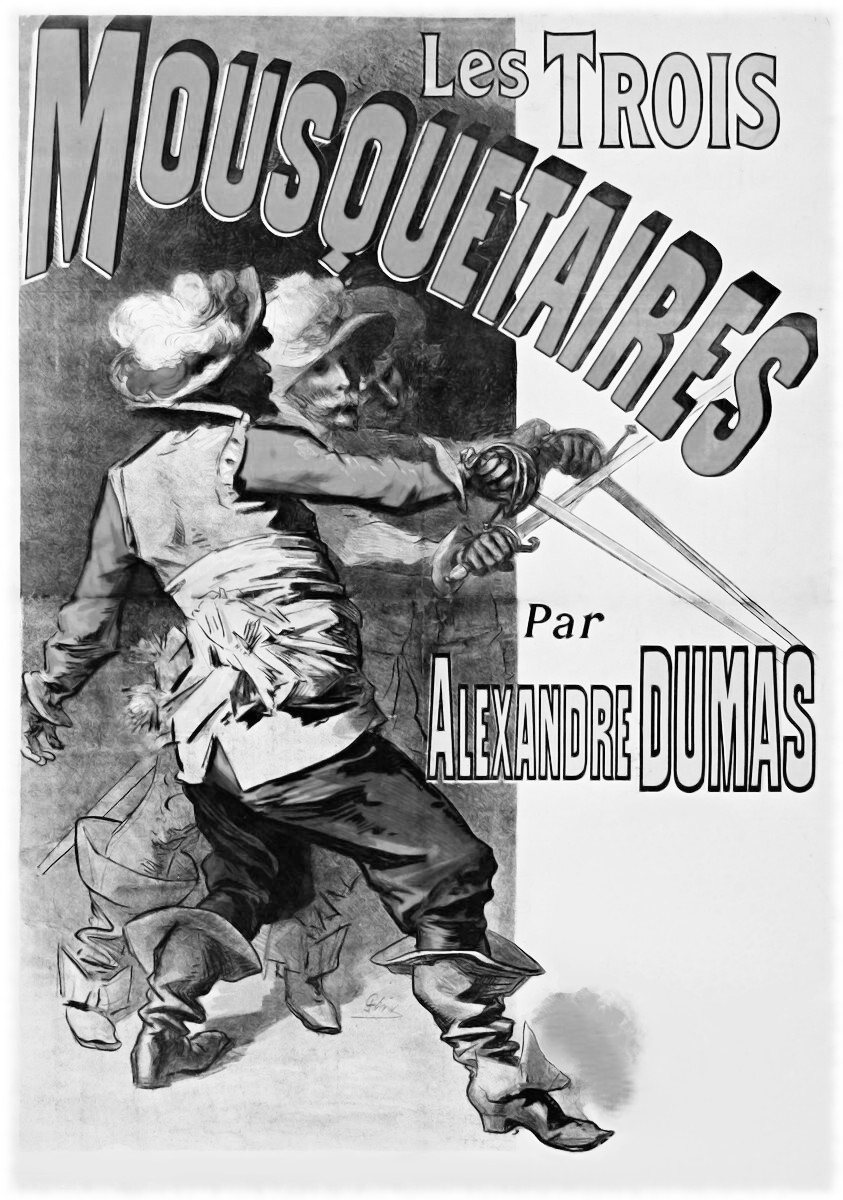
\includepdf[width=1.3\textwidth]{titlepage.jpg}
\tableofcontents
 
 \renewcommand{\chaptermark}[1]{\markboth{#1}{}}
 %!TeX root=../musketeerstop.tex 

\addchap{Author's Preface} 	

\begin{center}\scshape
In which it is proved that, notwithstanding their names' ending in \textit{os} and \textit{is}, the heroes of the story which we are about to have the honour to relate to our readers have nothing mythological about them. 
\end{center}
	
	A short time ago, while making researches in the Royal Library for my History of Louis XIV, I stumbled by chance upon the Memoirs of M. d'Artagnan, printed---as were most of the works of that period, in which authors could not tell the truth without the risk of a residence, more or less long, in the Bastille---at Amsterdam, by Pierre Rouge. The title attracted me; I took them home with me, with the permission of the guardian, and devoured them. 

It is not my intention here to enter into an analysis of this curious work; and I shall satisfy myself with referring such of my readers as appreciate the pictures of the period to its pages. They will therein find portraits pencilled by the hand of a master; and although these squibs may be, for the most part, traced upon the doors of barracks and the walls of cabarets, they will not find the likenesses of Louis XIII., Anne of Austria, Richelieu, Mazarin, and the courtiers of the period, less faithful than in the history of M. Anquetil. 

But, it is well known, what strikes the capricious mind of the poet is not always what affects the mass of readers. Now, while admiring, as others doubtless will admire, the details we have to relate, our main preoccupation concerned a matter to which no one before ourselves had given a thought. 

D'Artagnan relates that on his first visit to M. de Tréville, captain of the king's Musketeers, he met in the antechamber three young men, serving in the illustrious corps into which he was soliciting the honour of being received, bearing the names of Athos, Porthos, and Aramis. 

We must confess these three strange names struck us; and it immediately occurred to us that they were but pseudonyms, under which d'Artagnan had disguised names perhaps illustrious, or else that the bearers of these borrowed names had themselves chosen them on the day in which, from caprice, discontent, or want of fortune, they had donned the simple Musketeer's uniform. 

From that moment we had no rest till we could find some trace in contemporary works of these extraordinary names which had so strongly awakened our curiosity. 

The catalogue alone of the books we read with this object would fill a whole chapter, which, although it might be very instructive, would certainly afford our readers but little amusement. It will suffice, then, to tell them that at the moment at which, discouraged by so many fruitless investigations, we were about to abandon our search, we at length found, guided by the counsels of our illustrious friend Paulin Paris, a manuscript in folio, endorsed 4772 or 4773, we do not recollect which, having for title, <Memoirs of the Comte de la Fère, Touching Some Events Which Passed in France Toward the End of the Reign of King Louis XIII and the Commencement of the Reign of King Louis XIV.>

It may be easily imagined how great was our joy when, in turning over this manuscript, our last hope, we found at the twentieth page the name of Athos, at the twenty-seventh the name of Porthos, and at the thirty-first the name of Aramis. 

The discovery of a completely unknown manuscript at a period in which historical science is carried to such a high degree appeared almost miraculous. We hastened, therefore, to obtain permission to print it, with the view of presenting ourselves someday with the pack of others at the doors of the Académie des Inscriptions et Belles Lettres, if we should not succeed---a very probable thing, by the by---in gaining admission to the Académie Française with our own proper pack. This permission, we feel bound to say, was graciously granted; which compels us here to give a public contradiction to the slanderers who pretend that we live under a government but moderately indulgent to men of letters. 

Now, this is the first part of this precious manuscript which we offer to our readers, restoring it to the title which belongs to it, and entering into an engagement that if (of which we have no doubt) this first part should obtain the success it merits, we will publish the second immediately. 

In the meanwhile, as the godfather is a second father, we beg the reader to lay to our account, and not to that of the Comte de la Fère, the pleasure or the \textit{ennui} he may experience. 

This being understood, let us proceed with our history.
 \renewcommand{\chaptermark}[1]{\markboth{\chaptername\ \arabic{chapter}:\ #1}{}}
 
\mainmatter
\pagestyle{headings}
\KOMAoptions{headings=openright}

%!TeX root=../musketeerstop.tex 

\chapter{The Three Presents of D'Artagnan the Elder}

\lettrine[]{O}{n} the first Monday of the month of April, 1625, the market town of Meung, in which the author of \textit{Romance of the Rose} was born, appeared to be in as perfect a state of revolution as if the Huguenots had just made a second La Rochelle of it. Many citizens, seeing the women flying toward the High Street, leaving their children crying at the open doors, hastened to don the cuirass, and supporting their somewhat uncertain courage with a musket or a partisan, directed their steps toward the hostelry of the Jolly Miller, before which was gathered, increasing every minute, a compact group, vociferous and full of curiosity. 

In those times panics were common, and few days passed without some city or other registering in its archives an event of this kind. There were nobles, who made war against each other; there was the king, who made war against the cardinal; there was Spain, which made war against the king. Then, in addition to these concealed or public, secret or open wars, there were robbers, mendicants, Huguenots, wolves, and scoundrels, who made war upon everybody. The citizens always took up arms readily against thieves, wolves or scoundrels, often against nobles or Huguenots, sometimes against the king, but never against the cardinal or Spain. It resulted, then, from this habit that on the said first Monday of April, 1625, the citizens, on hearing the clamour, and seeing neither the red-and-yellow standard nor the livery of the Duc de Richelieu, rushed toward the hostel of the Jolly Miller. When arrived there, the cause of the hubbub was apparent to all. 

A young man---we can sketch his portrait at a dash. Imagine to yourself a Don Quixote of eighteen; a Don Quixote without his corselet, without his coat of mail, without his cuisses; a Don Quixote clothed in a woollen doublet, the blue colour of which had faded into a nameless shade between lees of wine and a heavenly azure; face long and brown; high cheek bones, a sign of sagacity; the maxillary muscles enormously developed, an infallible sign by which a Gascon may always be detected, even without his cap---and our young man wore a cap set off with a sort of feather; the eye open and intelligent; the nose hooked, but finely chiselled. Too big for a youth, too small for a grown man, an experienced eye might have taken him for a farmer's son upon a journey had it not been for the long sword which, dangling from a leather baldric, hit against the calves of its owner as he walked, and against the rough side of his steed when he was on horseback. 

For our young man had a steed which was the observed of all observers. It was a Béarn pony, from twelve to fourteen years old, yellow in his hide, without a hair in his tail, but not without windgalls on his legs, which, though going with his head lower than his knees, rendering a martingale quite unnecessary, contrived nevertheless to perform his eight leagues a day. Unfortunately, the qualities of this horse were so well concealed under his strange-coloured hide and his unaccountable gait, that at a time when everybody was a connoisseur in horseflesh, the appearance of the aforesaid pony at Meung---which place he had entered about a quarter of an hour before, by the gate of Beaugency---produced an unfavourable feeling, which extended to his rider. 

And this feeling had been more painfully perceived by young d'Artagnan---for so was the Don Quixote of this second Rosinante named---from his not being able to conceal from himself the ridiculous appearance that such a steed gave him, good horseman as he was. He had sighed deeply, therefore, when accepting the gift of the pony from M. d'Artagnan the elder. He was not ignorant that such a beast was worth at least twenty livres; and the words which had accompanied the present were above all price. 

<My son,> said the old Gascon gentleman, in that pure Béarn \textit{patois} of which Henry IV could never rid himself, <this horse was born in the house of your father about thirteen years ago, and has remained in it ever since, which ought to make you love it. Never sell it; allow it to die tranquilly and honourably of old age, and if you make a campaign with it, take as much care of it as you would of an old servant. At court, provided you have ever the honour to go there,> continued M. d'Artagnan the elder, <---an honour to which, remember, your ancient nobility gives you the right---sustain worthily your name of gentleman, which has been worthily borne by your ancestors for five hundred years, both for your own sake and the sake of those who belong to you. By the latter I mean your relatives and friends. Endure nothing from anyone except Monsieur the Cardinal and the king. It is by his courage, please observe, by his courage alone, that a gentleman can make his way nowadays. Whoever hesitates for a second perhaps allows the bait to escape which during that exact second fortune held out to him. You are young. You ought to be brave for two reasons: the first is that you are a Gascon, and the second is that you are my son. Never fear quarrels, but seek adventures. I have taught you how to handle a sword; you have thews of iron, a wrist of steel. Fight on all occasions. Fight the more for duels being forbidden, since consequently there is twice as much courage in fighting. I have nothing to give you, my son, but fifteen crowns, my horse, and the counsels you have just heard. Your mother will add to them a recipe for a certain balsam, which she had from a Bohemian and which has the miraculous virtue of curing all wounds that do not reach the heart. Take advantage of all, and live happily and long. I have but one word to add, and that is to propose an example to you---not mine, for I myself have never appeared at court, and have only taken part in religious wars as a volunteer; I speak of Monsieur de Tréville, who was formerly my neighbour, and who had the honour to be, as a child, the play-fellow of our king, Louis XIII, whom God preserve! Sometimes their play degenerated into battles, and in these battles the king was not always the stronger. The blows which he received increased greatly his esteem and friendship for Monsieur de Tréville. Afterward, Monsieur de Tréville fought with others: in his first journey to Paris, five times; from the death of the late king till the young one came of age, without reckoning wars and sieges, seven times; and from that date up to the present day, a hundred times, perhaps! So that in spite of edicts, ordinances, and decrees, there he is, captain of the Musketeers; that is to say, chief of a legion of Cæsars, whom the king holds in great esteem and whom the cardinal dreads---he who dreads nothing, as it is said. Still further, Monsieur de Tréville gains ten thousand crowns a year; he is therefore a great noble. He began as you begin. Go to him with this letter, and make him your model in order that you may do as he has done.> 

Upon which M. d'Artagnan the elder girded his own sword round his son, kissed him tenderly on both cheeks, and gave him his benediction. 

On leaving the paternal chamber, the young man found his mother, who was waiting for him with the famous recipe of which the counsels we have just repeated would necessitate frequent employment. The adieux were on this side longer and more tender than they had been on the other---not that M. d'Artagnan did not love his son, who was his only offspring, but M. d'Artagnan was a man, and he would have considered it unworthy of a man to give way to his feelings; whereas Mme. d'Artagnan was a woman, and still more, a mother. She wept abundantly; and---let us speak it to the praise of M. d'Artagnan the younger---notwithstanding the efforts he made to remain firm, as a future Musketeer ought, nature prevailed, and he shed many tears, of which he succeeded with great difficulty in concealing the half. 

The same day the young man set forward on his journey, furnished with the three paternal gifts, which consisted, as we have said, of fifteen crowns, the horse, and the letter for M. de Tréville---the counsels being thrown into the bargain. 

With such a \textit{vade mecum} D'Artagnan was morally and physically an exact copy of the hero of Cervantes, to whom we so happily compared him when our duty of an historian placed us under the necessity of sketching his portrait. Don Quixote took windmills for giants, and sheep for armies; d'Artagnan took every smile for an insult, and every look as a provocation---whence it resulted that from Tarbes to Meung his fist was constantly doubled, or his hand on the hilt of his sword; and yet the fist did not descend upon any jaw, nor did the sword issue from its scabbard. It was not that the sight of the wretched pony did not excite numerous smiles on the countenances of passers-by; but as against the side of this pony rattled a sword of respectable length, and as over this sword gleamed an eye rather ferocious than haughty, these passers-by repressed their hilarity, or if hilarity prevailed over prudence, they endeavoured to laugh only on one side, like the masks of the ancients. D'Artagnan, then, remained majestic and intact in his susceptibility, till he came to this unlucky city of Meung. 

But there, as he was alighting from his horse at the gate of the Jolly Miller, without anyone---host, waiter, or hostler---coming to hold his stirrup or take his horse, d'Artagnan spied, though an open window on the ground floor, a gentleman, well-made and of good carriage, although of rather a stern countenance, talking with two persons who appeared to listen to him with respect. D'Artagnan fancied quite naturally, according to his custom, that he must be the object of their conversation, and listened. This time d'Artagnan was only in part mistaken; he himself was not in question, but his horse was. The gentleman appeared to be enumerating all his qualities to his auditors; and, as I have said, the auditors seeming to have great deference for the narrator, they every moment burst into fits of laughter. Now, as a half-smile was sufficient to awaken the irascibility of the young man, the effect produced upon him by this vociferous mirth may be easily imagined. 

Nevertheless, d'Artagnan was desirous of examining the appearance of this impertinent personage who ridiculed him. He fixed his haughty eye upon the stranger, and perceived a man of from forty to forty-five years of age, with black and piercing eyes, pale complexion, a strongly marked nose, and a black and well-shaped moustache. He was dressed in a doublet and hose of a violet colour, with aiguillettes of the same colour, without any other ornaments than the customary slashes, through which the shirt appeared. This doublet and hose, though new, were creased, like travelling clothes for a long time packed in a portmanteau. D'Artagnan made all these remarks with the rapidity of a most minute observer, and doubtless from an instinctive feeling that this stranger was destined to have a great influence over his future life. 

Now, as at the moment in which d'Artagnan fixed his eyes upon the gentleman in the violet doublet, the gentleman made one of his most knowing and profound remarks respecting the Béarnese pony, his two auditors laughed even louder than before, and he himself, though contrary to his custom, allowed a pale smile (if I may be allowed to use such an expression) to stray over his countenance. This time there could be no doubt; d'Artagnan was really insulted. Full, then, of this conviction, he pulled his cap down over his eyes, and endeavouring to copy some of the court airs he had picked up in Gascony among young travelling nobles, he advanced with one hand on the hilt of his sword and the other resting on his hip. Unfortunately, as he advanced, his anger increased at every step; and instead of the proper and lofty speech he had prepared as a prelude to his challenge, he found nothing at the tip of his tongue but a gross personality, which he accompanied with a furious gesture. 

<I say, sir, you sir, who are hiding yourself behind that shutter---yes, you, sir, tell me what you are laughing at, and we will laugh together!> 

The gentleman raised his eyes slowly from the nag to his cavalier, as if he required some time to ascertain whether it could be to him that such strange reproaches were addressed; then, when he could not possibly entertain any doubt of the matter, his eyebrows slightly bent, and with an accent of irony and insolence impossible to be described, he replied to d'Artagnan, <I was not speaking to you, sir.> 

<But I am speaking to you!> replied the young man, additionally exasperated with this mixture of insolence and good manners, of politeness and scorn. 

The stranger looked at him again with a slight smile, and retiring from the window, came out of the hostelry with a slow step, and placed himself before the horse, within two paces of d'Artagnan. His quiet manner and the ironical expression of his countenance redoubled the mirth of the persons with whom he had been talking, and who still remained at the window. 

D'Artagnan, seeing him approach, drew his sword a foot out of the scabbard. 

<This horse is decidedly, or rather has been in his youth, a buttercup,> resumed the stranger, continuing the remarks he had begun, and addressing himself to his auditors at the window, without paying the least attention to the exasperation of d'Artagnan, who, however, placed himself between him and them. <It is a colour very well known in botany, but till the present time very rare among horses.> 

<There are people who laugh at the horse that would not dare to laugh at the master,> cried the young emulator of the furious Tréville. 

<I do not often laugh, sir,> replied the stranger, <as you may perceive by the expression of my countenance; but nevertheless I retain the privilege of laughing when I please.> 

<And I,> cried d'Artagnan, <will allow no man to laugh when it displeases me!> 

<Indeed, sir,> continued the stranger, more calm than ever; <well, that is perfectly right!> and turning on his heel, was about to re-enter the hostelry by the front gate, beneath which d'Artagnan on arriving had observed a saddled horse. 

But, d'Artagnan was not of a character to allow a man to escape him thus who had the insolence to ridicule him. He drew his sword entirely from the scabbard, and followed him, crying, <Turn, turn, Master Joker, lest I strike you behind!> 

<Strike me!> said the other, turning on his heels, and surveying the young man with as much astonishment as contempt. <Why, my good fellow, you must be mad!> Then, in a suppressed tone, as if speaking to himself, <This is annoying,> continued he. <What a godsend this would be for his Majesty, who is seeking everywhere for brave fellows to recruit for his Musketeers!> 

He had scarcely finished, when d'Artagnan made such a furious lunge at him that if he had not sprung nimbly backward, it is probable he would have jested for the last time. The stranger, then perceiving that the matter went beyond raillery, drew his sword, saluted his adversary, and seriously placed himself on guard. But at the same moment, his two auditors, accompanied by the host, fell upon d'Artagnan with sticks, shovels and tongs. This caused so rapid and complete a diversion from the attack that d'Artagnan's adversary, while the latter turned round to face this shower of blows, sheathed his sword with the same precision, and instead of an actor, which he had nearly been, became a spectator of the fight---a part in which he acquitted himself with his usual impassiveness, muttering, nevertheless, <A plague upon these Gascons! Replace him on his orange horse, and let him begone!> 

<Not before I have killed you, poltroon!> cried d'Artagnan, making the best face possible, and never retreating one step before his three assailants, who continued to shower blows upon him. 

<Another gasconade!> murmured the gentleman. <By my honour, these Gascons are incorrigible! Keep up the dance, then, since he will have it so. When he is tired, he will perhaps tell us that he has had enough of it.> 

But the stranger knew not the headstrong personage he had to do with; d'Artagnan was not the man ever to cry for quarter. The fight was therefore prolonged for some seconds; but at length d'Artagnan dropped his sword, which was broken in two pieces by the blow of a stick. Another blow full upon his forehead at the same moment brought him to the ground, covered with blood and almost fainting. 

It was at this moment that people came flocking to the scene of action from all sides. The host, fearful of consequences, with the help of his servants carried the wounded man into the kitchen, where some trifling attentions were bestowed upon him. 

As to the gentleman, he resumed his place at the window, and surveyed the crowd with a certain impatience, evidently annoyed by their remaining undispersed. 

<Well, how is it with this madman?> exclaimed he, turning round as the noise of the door announced the entrance of the host, who came in to inquire if he was unhurt. 

<Your Excellency is safe and sound?> asked the host. 

<Oh, yes! Perfectly safe and sound, my good host; and I wish to know what has become of our young man.> 

<He is better,> said the host, <he fainted quite away.> 

<Indeed!> said the gentleman. 

<But before he fainted, he collected all his strength to challenge you, and to defy you while challenging you.> 

<Why, this fellow must be the devil in person!> cried the stranger. 

<Oh, no, your Excellency, he is not the devil,> replied the host, with a grin of contempt; <for during his fainting we rummaged his valise and found nothing but a clean shirt and eleven crowns---which however, did not prevent his saying, as he was fainting, that if such a thing had happened in Paris, you should have cause to repent of it at a later period.> 

<Then,> said the stranger coolly, <he must be some prince in disguise.> 

<I have told you this, good sir,> resumed the host, <in order that you may be on your guard.> 

<Did he name no one in his passion?> 

<Yes; he struck his pocket and said, <We shall see what Monsieur de Tréville will think of this insult offered to his \textit{protégé}.>> 

<Monsieur de Tréville?> said the stranger, becoming attentive, <he put his hand upon his pocket while pronouncing the name of Monsieur de Tréville? Now, my dear host, while your young man was insensible, you did not fail, I am quite sure, to ascertain what that pocket contained. What was there in it?> 

<A letter addressed to Monsieur de Tréville, captain of the Musketeers.> 

<Indeed!> 

<Exactly as I have the honour to tell your Excellency.> 

The host, who was not endowed with great perspicacity, did not observe the expression which his words had given to the physiognomy of the stranger. The latter rose from the front of the window, upon the sill of which he had leaned with his elbow, and knitted his brow like a man disquieted. 

<The devil!> murmured he, between his teeth. <Can Tréville have set this Gascon upon me? He is very young; but a sword thrust is a sword thrust, whatever be the age of him who gives it, and a youth is less to be suspected than an older man,> and the stranger fell into a reverie which lasted some minutes. <A weak obstacle is sometimes sufficient to overthrow a great design.>

<Host,> said he, <could you not contrive to get rid of this frantic boy for me? In conscience, I cannot kill him; and yet,> added he, with a coldly menacing expression, <he annoys me. Where is he?> 

<In my wife's chamber, on the first flight, where they are dressing his wounds.> 

<His things and his bag are with him? Has he taken off his doublet?> 

<On the contrary, everything is in the kitchen. But if he annoys you, this young fool\longdash> 

<To be sure he does. He causes a disturbance in your hostelry, which respectable people cannot put up with. Go; make out my bill and notify my servant.> 

<What, monsieur, will you leave us so soon?> 

<You know that very well, as I gave my order to saddle my horse. Have they not obeyed me?> 

<It is done; as your Excellency may have observed, your horse is in the great gateway, ready saddled for your departure.> 

<That is well; do as I have directed you, then.> 

<What the devil!> said the host to himself. <Can he be afraid of this boy?> But an imperious glance from the stranger stopped him short; he bowed humbly and retired. 

<It is not necessary for Milady\footnote{We are well aware that this term, milady, is only properly used when followed by a family name. But we find it thus in the manuscript, and we do not choose to take upon ourselves to alter it.} to be seen by this fellow,> continued the stranger. <She will soon pass; she is already late. I had better get on horseback, and go and meet her. I should like, however, to know what this letter addressed to Tréville contains.> And the stranger, muttering to himself, directed his steps toward the kitchen.

In the meantime, the host, who entertained no doubt that it was the presence of the young man that drove the stranger from his hostelry, re-ascended to his wife's chamber, and found d'Artagnan just recovering his senses. Giving him to understand that the police would deal with him pretty severely for having sought a quarrel with a great lord---for in the opinion of the host the stranger could be nothing less than a great lord---he insisted that notwithstanding his weakness d'Artagnan should get up and depart as quickly as possible. D'Artagnan, half stupefied, without his doublet, and with his head bound up in a linen cloth, arose then, and urged by the host, began to descend the stairs; but on arriving at the kitchen, the first thing he saw was his antagonist talking calmly at the step of a heavy carriage, drawn by two large Norman horses. 

His interlocutor, whose head appeared through the carriage window, was a woman of from twenty to two-and-twenty years. We have already observed with what rapidity d'Artagnan seized the expression of a countenance. He perceived then, at a glance, that this woman was young and beautiful; and her style of beauty struck him more forcibly from its being totally different from that of the southern countries in which d'Artagnan had hitherto resided. She was pale and fair, with long curls falling in profusion over her shoulders, had large, blue, languishing eyes, rosy lips, and hands of alabaster. She was talking with great animation with the stranger. 

<His Eminence, then, orders me\longdash> said the lady. 

<To return instantly to England, and to inform him as soon as the duke leaves London.> 

<And as to my other instructions?> asked the fair traveller. 

<They are contained in this box, which you will not open until you are on the other side of the Channel.> 

<Very well; and you---what will you do?> 

<I---I return to Paris.> 

<What, without chastising this insolent boy?> asked the lady. 

The stranger was about to reply; but at the moment he opened his mouth, d'Artagnan, who had heard all, precipitated himself over the threshold of the door. 

<This insolent boy chastises others,> cried he; <and I hope that this time he whom he ought to chastise will not escape him as before.> 

<Will not escape him?> replied the stranger, knitting his brow. 

<No; before a woman you would dare not fly, I presume?> 

<Remember,> said Milady, seeing the stranger lay his hand on his sword, <the least delay may ruin everything.> 

<You are right,> cried the gentleman; <begone then, on your part, and I will depart as quickly on mine.> And bowing to the lady, he sprang into his saddle, while her coachman applied his whip vigorously to his horses. The two interlocutors thus separated, taking opposite directions, at full gallop. 

<Pay him, booby!> cried the stranger to his servant, without checking the speed of his horse; and the man, after throwing two or three silver pieces at the foot of mine host, galloped after his master. 

<Base coward! false gentleman!> cried d'Artagnan, springing forward, in his turn, after the servant. But his wound had rendered him too weak to support such an exertion. Scarcely had he gone ten steps when his ears began to tingle, a faintness seized him, a cloud of blood passed over his eyes, and he fell in the middle of the street, crying still, <Coward! coward! coward!> 

<He is a coward, indeed,> grumbled the host, drawing near to d'Artagnan, and endeavouring by this little flattery to make up matters with the young man, as the heron of the fable did with the snail he had despised the evening before. 

<Yes, a base coward,> murmured d'Artagnan; <but she---she was very beautiful.> 

<What \textit{she?}> demanded the host. 

<Milady,> faltered d'Artagnan, and fainted a second time. 

<Ah, it's all one,> said the host; <I have lost two customers, but this one remains, of whom I am pretty certain for some days to come. There will be eleven crowns gained.> 

It is to be remembered that eleven crowns was just the sum that remained in d'Artagnan's purse. 

The host had reckoned upon eleven days of confinement at a crown a day, but he had reckoned without his guest. On the following morning at five o'clock d'Artagnan arose, and descending to the kitchen without help, asked, among other ingredients the list of which has not come down to us, for some oil, some wine, and some rosemary, and with his mother's recipe in his hand composed a balsam, with which he anointed his numerous wounds, replacing his bandages himself, and positively refusing the assistance of any doctor, d'Artagnan walked about that same evening, and was almost cured by the morrow. 

But when the time came to pay for his rosemary, this oil, and the wine, the only expense the master had incurred, as he had preserved a strict abstinence---while on the contrary, the yellow horse, by the account of the hostler at least, had eaten three times as much as a horse of his size could reasonably be supposed to have done---D'Artagnan found nothing in his pocket but his little old velvet purse with the eleven crowns it contained; for as to the letter addressed to M. de Tréville, it had disappeared. 

The young man commenced his search for the letter with the greatest patience, turning out his pockets of all kinds over and over again, rummaging and rerummaging in his valise, and opening and reopening his purse; but when he found that he had come to the conviction that the letter was not to be found, he flew, for the third time, into such a rage as was near costing him a fresh consumption of wine, oil, and rosemary---for upon seeing this hot-headed youth become exasperated and threaten to destroy everything in the establishment if his letter were not found, the host seized a spit, his wife a broom handle, and the servants the same sticks they had used the day before. 

<My letter of recommendation!> cried d'Artagnan, <my letter of recommendation! or, the holy blood, I will spit you all like ortolans!> 

Unfortunately, there was one circumstance which created a powerful obstacle to the accomplishment of this threat; which was, as we have related, that his sword had been in his first conflict broken in two, and which he had entirely forgotten. Hence, it resulted when d'Artagnan proceeded to draw his sword in earnest, he found himself purely and simply armed with a stump of a sword about eight or ten inches in length, which the host had carefully placed in the scabbard. As to the rest of the blade, the master had slyly put that on one side to make himself a larding pin. 

But this deception would probably not have stopped our fiery young man if the host had not reflected that the reclamation which his guest made was perfectly just. 

<But, after all,> said he, lowering the point of his spit, <where is this letter?> 

<Yes, where is this letter?> cried d'Artagnan. <In the first place, I warn you that that letter is for Monsieur de Tréville, and it must be found, or if it is not found, he will know how to find it.> 

His threat completed the intimidation of the host. After the king and the cardinal, M. de Tréville was the man whose name was perhaps most frequently repeated by the military, and even by citizens. There was, to be sure, Father Joseph, but his name was never pronounced but with a subdued voice, such was the terror inspired by his Gray Eminence, as the cardinal's familiar was called. 

Throwing down his spit, and ordering his wife to do the same with her broom handle, and the servants with their sticks, he set the first example of commencing an earnest search for the lost letter. 

<Does the letter contain anything valuable?> demanded the host, after a few minutes of useless investigation. 

<Zounds! I think it does indeed!> cried the Gascon, who reckoned upon this letter for making his way at court. <It contained my fortune!> 

<Bills upon Spain?> asked the disturbed host. 

<Bills upon his Majesty's private treasury,> answered d'Artagnan, who, reckoning upon entering into the king's service in consequence of this recommendation, believed he could make this somewhat hazardous reply without telling of a falsehood. 

<The devil!> cried the host, at his wits' end. 

<But it's of no importance,> continued d'Artagnan, with natural assurance; <it's of no importance. The money is nothing; that letter was everything. I would rather have lost a thousand pistoles than have lost it.> He would not have risked more if he had said twenty thousand; but a certain juvenile modesty restrained him. 

A ray of light all at once broke upon the mind of the host as he was giving himself to the devil upon finding nothing. 

<That letter is not lost!> cried he. 

<What!> cried d'Artagnan. 

<No, it has been stolen from you.> 

<Stolen? By whom?> 

<By the gentleman who was here yesterday. He came down into the kitchen, where your doublet was. He remained there some time alone. I would lay a wager he has stolen it.> 

<Do you think so?> answered d'Artagnan, but little convinced, as he knew better than anyone else how entirely personal the value of this letter was, and saw nothing in it likely to tempt cupidity. The fact was that none of his servants, none of the travellers present, could have gained anything by being possessed of this paper. 

<Do you say,> resumed d'Artagnan, <that you suspect that impertinent gentleman?> 

<I tell you I am sure of it,> continued the host. <When I informed him that your lordship was the \textit{protégé} of Monsieur de Tréville, and that you even had a letter for that illustrious gentleman, he appeared to be very much disturbed, and asked me where that letter was, and immediately came down into the kitchen, where he knew your doublet was.> 

<Then that's my thief,> replied d'Artagnan. <I will complain to Monsieur de Tréville, and Monsieur de Tréville will complain to the king.> He then drew two crowns majestically from his purse and gave them to the host, who accompanied him, cap in hand, to the gate, and remounted his yellow horse, which bore him without any further accident to the gate of St. Antoine at Paris, where his owner sold him for three crowns, which was a very good price, considering that d'Artagnan had ridden him hard during the last stage. Thus the dealer to whom d'Artagnan sold him for the nine livres did not conceal from the young man that he only gave that enormous sum for him on the account of the originality of his colour. 

Thus d'Artagnan entered Paris on foot, carrying his little packet under his arm, and walked about till he found an apartment to be let on terms suited to the scantiness of his means. This chamber was a sort of garret, situated in the Rue des Fossoyeurs, near the Luxembourg. 

As soon as the earnest money was paid, d'Artagnan took possession of his lodging, and passed the remainder of the day in sewing onto his doublet and hose some ornamental braiding which his mother had taken off an almost-new doublet of the elder M. d'Artagnan, and which she had given her son secretly. Next he went to the Quai de Feraille to have a new blade put to his sword, and then returned toward the Louvre, inquiring of the first Musketeer he met for the situation of the hôtel of M. de Tréville, which proved to be in the Rue du Vieux-Colombier; that is to say, in the immediate vicinity of the chamber hired by d'Artagnan---a circumstance which appeared to furnish a happy augury for the success of his journey. 

After this, satisfied with the way in which he had conducted himself at Meung, without remorse for the past, confident in the present, and full of hope for the future, he retired to bed and slept the sleep of the brave. 

This sleep, provincial as it was, brought him to nine o'clock in the morning; at which hour he rose, in order to repair to the residence of M. de Tréville, the third personage in the kingdom, in the paternal estimation.
%!TeX root=../musketeerstop.tex 

\chapter{The Antechamber of M. de Tréville} 
	
	\lettrine[]{M}{.} de Troisville, as his family was still called in Gascony, or M. de Tréville, as he has ended by styling himself in Paris, had really commenced life as d'Artagnan now did; that is to say, without a sou in his pocket, but with a fund of audacity, shrewdness, and intelligence which makes the poorest Gascon gentleman often derive more in his hope from the paternal inheritance than the richest Perigordian or Berrichan gentleman derives in reality from his. His insolent bravery, his still more insolent success at a time when blows poured down like hail, had borne him to the top of that difficult ladder called Court Favour, which he had climbed four steps at a time. 

He was the friend of the king, who honoured highly, as everyone knows, the memory of his father, Henry IV The father of M. de Tréville had served him so faithfully in his wars against the league that in default of money---a thing to which the Béarnais was accustomed all his life, and who constantly paid his debts with that of which he never stood in need of borrowing, that is to say, with ready wit---in default of money, we repeat, he authorized him, after the reduction of Paris, to assume for his arms a golden lion passant upon gules, with the motto \textit{Fidelis et fortis}. This was a great matter in the way of honour, but very little in the way of wealth; so that when the illustrious companion of the great Henry died, the only inheritance he was able to leave his son was his sword and his motto. Thanks to this double gift and the spotless name that accompanied it, M. de Tréville was admitted into the household of the young prince where he made such good use of his sword, and was so faithful to his motto, that Louis XIII, one of the good blades of his kingdom, was accustomed to say that if he had a friend who was about to fight, he would advise him to choose as a second, himself first, and Tréville next---or even, perhaps, before himself. 

Thus Louis XIII had a real liking for Tréville---a royal liking, a self-interested liking, it is true, but still a liking. At that unhappy period it was an important consideration to be surrounded by such men as Tréville. Many might take for their device the epithet \textit{strong}, which formed the second part of his motto, but very few gentlemen could lay claim to the \textit{faithful}, which constituted the first. Tréville was one of these latter. His was one of those rare organizations, endowed with an obedient intelligence like that of the dog; with a blind valour, a quick eye, and a prompt hand; to whom sight appeared only to be given to see if the king were dissatisfied with anyone, and the hand to strike this displeasing personage, whether a Besme, a Maurevers, a Poltiot de Méré, or a Vitry. In short, up to this period nothing had been wanting to Tréville but opportunity; but he was ever on the watch for it, and he faithfully promised himself that he would not fail to seize it by its three hairs whenever it came within reach of his hand. At last Louis XIII made Tréville the captain of his Musketeers, who were to Louis XIII in devotedness, or rather in fanaticism, what his Ordinaries had been to Henry III, and his Scotch Guard to Louis XI. 

On his part, the cardinal was not behind the king in this respect. When he saw the formidable and chosen body with which Louis XIII had surrounded himself, this second, or rather this first king of France, became desirous that he, too, should have his guard. He had his Musketeers therefore, as Louis XIII had his, and these two powerful rivals vied with each other in procuring, not only from all the provinces of France, but even from all foreign states, the most celebrated swordsmen. It was not uncommon for Richelieu and Louis XIII to dispute over their evening game of chess upon the merits of their servants. Each boasted the bearing and the courage of his own people. While exclaiming loudly against duels and brawls, they excited them secretly to quarrel, deriving an immoderate satisfaction or genuine regret from the success or defeat of their own combatants. We learn this from the memoirs of a man who was concerned in some few of these defeats and in many of these victories. 

Tréville had grasped the weak side of his master; and it was to this address that he owed the long and constant favour of a king who has not left the reputation behind him of being very faithful in his friendships. He paraded his Musketeers before the Cardinal Armand Duplessis with an insolent air which made the gray moustache of his Eminence curl with ire. Tréville understood admirably the war method of that period, in which he who could not live at the expense of the enemy must live at the expense of his compatriots. His soldiers formed a legion of devil-may-care fellows, perfectly undisciplined toward all but himself. 

Loose, half-drunk, imposing, the king's Musketeers, or rather M. de Tréville's, spread themselves about in the cabarets, in the public walks, and the public sports, shouting, twisting their moustaches, clanking their swords, and taking great pleasure in annoying the Guards of the cardinal whenever they could fall in with them; then drawing in the open streets, as if it were the best of all possible sports; sometimes killed, but sure in that case to be both wept and avenged; often killing others, but then certain of not rotting in prison, M. de Tréville being there to claim them. Thus M. de Tréville was praised to the highest note by these men, who adored him, and who, ruffians as they were, trembled before him like scholars before their master, obedient to his least word, and ready to sacrifice themselves to wash out the smallest insult. 

M. de Tréville employed this powerful weapon for the king, in the first place, and the friends of the king---and then for himself and his own friends. For the rest, in the memoirs of this period, which has left so many memoirs, one does not find this worthy gentleman blamed even by his enemies; and he had many such among men of the pen as well as among men of the sword. In no instance, let us say, was this worthy gentleman accused of deriving personal advantage from the cooperation of his minions. Endowed with a rare genius for intrigue which rendered him the equal of the ablest intriguers, he remained an honest man. Still further, in spite of sword thrusts which weaken, and painful exercises which fatigue, he had become one of the most gallant frequenters of revels, one of the most insinuating lady's men, one of the softest whisperers of interesting nothings of his day; the \textit{bonnes fortunes} of de Tréville were talked of as those of M. de Bassompierre had been talked of twenty years before, and that was not saying a little. The captain of the Musketeers was therefore admired, feared, and loved; and this constitutes the zenith of human fortune. 

Louis XIV absorbed all the smaller stars of his court in his own vast radiance; but his father, a sun \textit{pluribus impar}, left his personal splendour to each of his favourites, his individual value to each of his courtiers. In addition to the levees of the king and the cardinal, there might be reckoned in Paris at that time more than two hundred smaller but still noteworthy levees. Among these two hundred levees, that of Tréville was one of the most sought. 

The court of his hôtel, situated in the Rue du Vieux-Colombier, resembled a camp from by six o'clock in the morning in summer and eight o'clock in winter. From fifty to sixty Musketeers, who appeared to replace one another in order always to present an imposing number, paraded constantly, armed to the teeth and ready for anything. On one of those immense staircases, upon whose space modern civilization would build a whole house, ascended and descended the office seekers of Paris, who ran after any sort of favour---gentlemen from the provinces anxious to be enrolled, and servants in all sorts of liveries, bringing and carrying messages between their masters and M. de Tréville. In the antechamber, upon long circular benches, reposed the elect; that is to say, those who were called. In this apartment a continued buzzing prevailed from morning till night, while M. de Tréville, in his office contiguous to this antechamber, received visits, listened to complaints, gave his orders, and like the king in his balcony at the Louvre, had only to place himself at the window to review both his men and arms. 

The day on which d'Artagnan presented himself the assemblage was imposing, particularly for a provincial just arriving from his province. It is true that this provincial was a Gascon; and that, particularly at this period, the compatriots of d'Artagnan had the reputation of not being easily intimidated. When he had once passed the massive door covered with long square-headed nails, he fell into the midst of a troop of swordsmen, who crossed one another in their passage, calling out, quarrelling, and playing tricks one with another. In order to make one's way amid these turbulent and conflicting waves, it was necessary to be an officer, a great noble, or a pretty woman. 

It was, then, into the midst of this tumult and disorder that our young man advanced with a beating heart, ranging his long rapier up his lanky leg, and keeping one hand on the edge of his cap, with that half-smile of the embarrassed provincial who wishes to put on a good face. When he had passed one group he began to breathe more freely; but he could not help observing that they turned round to look at him, and for the first time in his life d'Artagnan, who had till that day entertained a very good opinion of himself, felt ridiculous. 

Arrived at the staircase, it was still worse. There were four Musketeers on the bottom steps, amusing themselves with the following exercise, while ten or twelve of their comrades waited upon the landing place to take their turn in the sport. 

One of them, stationed upon the top stair, naked sword in hand, prevented, or at least endeavoured to prevent, the three others from ascending. 

These three others fenced against him with their agile swords. 

D'Artagnan at first took these weapons for foils, and believed them to be buttoned; but he soon perceived by certain scratches that every weapon was pointed and sharpened, and that at each of these scratches not only the spectators, but even the actors themselves, laughed like so many madmen. 

He who at the moment occupied the upper step kept his adversaries marvellously in check. A circle was formed around them. The conditions required that at every hit the man touched should quit the game, yielding his turn for the benefit of the adversary who had hit him. In five minutes three were slightly wounded, one on the hand, another on the ear, by the defender of the stair, who himself remained intact---a piece of skill which was worth to him, according to the rules agreed upon, three turns of favour. 

However difficult it might be, or rather as he pretended it was, to astonish our young traveller, this pastime really astonished him. He had seen in his province---that land in which heads become so easily heated---a few of the preliminaries of duels; but the daring of these four fencers appeared to him the strongest he had ever heard of even in Gascony. He believed himself transported into that famous country of giants into which Gulliver afterward went and was so frightened; and yet he had not gained the goal, for there were still the landing place and the antechamber. 

On the landing they were no longer fighting, but amused themselves with stories about women, and in the antechamber, with stories about the court. On the landing d'Artagnan blushed; in the antechamber he trembled. His warm and fickle imagination, which in Gascony had rendered him formidable to young chambermaids, and even sometimes their mistresses, had never dreamed, even in moments of delirium, of half the amorous wonders or a quarter of the feats of gallantry which were here set forth in connection with names the best known and with details the least concealed. But if his morals were shocked on the landing, his respect for the cardinal was scandalized in the antechamber. There, to his great astonishment, d'Artagnan heard the policy which made all Europe tremble criticized aloud and openly, as well as the private life of the cardinal, which so many great nobles had been punished for trying to pry into. That great man who was so revered by d'Artagnan the elder served as an object of ridicule to the Musketeers of Tréville, who cracked their jokes upon his bandy legs and his crooked back. Some sang ballads about Mme. d'Aguillon, his mistress, and Mme. Cambalet, his niece; while others formed parties and plans to annoy the pages and guards of the cardinal duke---all things which appeared to d'Artagnan monstrous impossibilities. 

Nevertheless, when the name of the king was now and then uttered unthinkingly amid all these cardinal jests, a sort of gag seemed to close for a moment on all these jeering mouths. They looked hesitatingly around them, and appeared to doubt the thickness of the partition between them and the office of M. de Tréville; but a fresh allusion soon brought back the conversation to his Eminence, and then the laughter recovered its loudness and the light was not withheld from any of his actions. 

<Certes, these fellows will all either be imprisoned or hanged,> thought the terrified d'Artagnan, <and I, no doubt, with them; for from the moment I have either listened to or heard them, I shall be held as an accomplice. What would my good father say, who so strongly pointed out to me the respect due to the cardinal, if he knew I was in the society of such pagans?> 

We have no need, therefore, to say that d'Artagnan dared not join in the conversation, only he looked with all his eyes and listened with all his ears, stretching his five senses so as to lose nothing; and despite his confidence on the paternal admonitions, he felt himself carried by his tastes and led by his instincts to praise rather than to blame the unheard-of things which were taking place. 

Although he was a perfect stranger in the court of M. de Tréville's courtiers, and this his first appearance in that place, he was at length noticed, and somebody came and asked him what he wanted. At this demand d'Artagnan gave his name very modestly, emphasized the title of compatriot, and begged the servant who had put the question to him to request a moment's audience of M. de Tréville---a request which the other, with an air of protection, promised to transmit in due season. 

D'Artagnan, a little recovered from his first surprise, had now leisure to study costumes and physiognomy. 

The centre of the most animated group was a Musketeer of great height and haughty countenance, dressed in a costume so peculiar as to attract general attention. He did not wear the uniform cloak---which was not obligatory at that epoch of less liberty but more independence---but a cerulean-blue doublet, a little faded and worn, and over this a magnificent baldric, worked in gold, which shone like water ripples in the sun. A long cloak of crimson velvet fell in graceful folds from his shoulders, disclosing in front the splendid baldric, from which was suspended a gigantic rapier. This Musketeer had just come off guard, complained of having a cold, and coughed from time to time affectedly. It was for this reason, as he said to those around him, that he had put on his cloak; and while he spoke with a lofty air and twisted his moustache disdainfully, all admired his embroidered baldric, and d'Artagnan more than anyone. 

<What would you have?> said the Musketeer. <This fashion is coming in. It is a folly, I admit, but still it is the fashion. Besides, one must lay out one's inheritance somehow.> 

<Ah, Porthos!> cried one of his companions, <don't try to make us believe you obtained that baldric by paternal generosity. It was given to you by that veiled lady I met you with the other Sunday, near the gate St. Honoré.> 

<No, upon honour and by the faith of a gentleman, I bought it with the contents of my own purse,> answered he whom they designated by the name Porthos. 

<Yes; about in the same manner,> said another Musketeer, <that I bought this new purse with what my mistress put into the old one.> 

<It's true, though,> said Porthos; <and the proof is that I paid twelve pistoles for it.> 

The wonder was increased, though the doubt continued to exist. 

<Is it not true, Aramis?> said Porthos, turning toward another Musketeer. 

This other Musketeer formed a perfect contrast to his interrogator, who had just designated him by the name of Aramis. He was a stout man, of about two- or three-and-twenty, with an open, ingenuous countenance, a black, mild eye, and cheeks rosy and downy as an autumn peach. His delicate moustache marked a perfectly straight line upon his upper lip; he appeared to dread to lower his hands lest their veins should swell, and he pinched the tips of his ears from time to time to preserve their delicate pink transparency. Habitually he spoke little and slowly, bowed frequently, laughed without noise, showing his teeth, which were fine and of which, as the rest of his person, he appeared to take great care. He answered the appeal of his friend by an affirmative nod of the head. 

This affirmation appeared to dispel all doubts with regard to the baldric. They continued to admire it, but said no more about it; and with a rapid change of thought, the conversation passed suddenly to another subject. 

<What do you think of the story Chalais's esquire relates?> asked another Musketeer, without addressing anyone in particular, but on the contrary speaking to everybody. 

<And what does he say?> asked Porthos, in a self-sufficient tone. 

<He relates that he met at Brussels Rochefort, the \textit{âme damnée} of the cardinal disguised as a Capuchin, and that this cursed Rochefort, thanks to his disguise, had tricked Monsieur de Laigues, like a ninny as he is.> 

<A ninny, indeed!> said Porthos; <but is the matter certain?> 

<I had it from Aramis,> replied the Musketeer. 

<Indeed?> 

<Why, you knew it, Porthos,> said Aramis. <I told you of it yesterday. Let us say no more about it.> 

<Say no more about it? That's \textit{your} opinion!> replied Porthos. 

<Say no more about it! \textit{Peste!} You come to your conclusions quickly. What! The cardinal sets a spy upon a gentleman, has his letters stolen from him by means of a traitor, a brigand, a rascal---has, with the help of this spy and thanks to this correspondence, Chalais's throat cut, under the stupid pretext that he wanted to kill the king and marry Monsieur to the queen! Nobody knew a word of this enigma. You unravelled it yesterday to the great satisfaction of all; and while we are still gaping with wonder at the news, you come and tell us today, <Let us say no more about it.>>

<Well, then, let us talk about it, since you desire it,> replied Aramis, patiently. 

<This Rochefort,> cried Porthos, <if I were the esquire of poor Chalais, should pass a minute or two very uncomfortably with me.> 

<And you---you would pass rather a sad quarter-hour with the Red Duke,> replied Aramis. 

<Oh, the Red Duke! Bravo! Bravo! The Red Duke!> cried Porthos, clapping his hands and nodding his head. <The Red Duke is capital. I'll circulate that saying, be assured, my dear fellow. Who says this Aramis is not a wit? What a misfortune it is you did not follow your first vocation; what a delicious abbé you would have made!> 

<Oh, it's only a temporary postponement,> replied Aramis; <I shall be one someday. You very well know, Porthos, that I continue to study theology for that purpose.> 

<He will be one, as he says,> cried Porthos; <he will be one, sooner or later.> 

<Sooner,> said Aramis. 

<He only waits for one thing to determine him to resume his cassock, which hangs behind his uniform,> said another Musketeer. 

<What is he waiting for?> asked another. 

<Only till the queen has given an heir to the crown of France.> 

<No jesting upon that subject, gentlemen,> said Porthos; <thank God the queen is still of an age to give one!> 

<They say that Monsieur de Buckingham is in France,> replied Aramis, with a significant smile which gave to this sentence, apparently so simple, a tolerably scandalous meaning. 

<Aramis, my good friend, this time you are wrong,> interrupted Porthos. <Your wit is always leading you beyond bounds; if Monsieur de Tréville heard you, you would repent of speaking thus.> 

<Are you going to give me a lesson, Porthos?> cried Aramis, from whose usually mild eye a flash passed like lightning. 

<My dear fellow, be a Musketeer or an abbé. Be one or the other, but not both,> replied Porthos. <You know what Athos told you the other day; you eat at everybody's mess. Ah, don't be angry, I beg of you, that would be useless; you know what is agreed upon between you, Athos and me. You go to Madame d'Aguillon's, and you pay your court to her; you go to Madame de Bois-Tracy's, the cousin of Madame de Chevreuse, and you pass for being far advanced in the good graces of that lady. Oh, good Lord! Don't trouble yourself to reveal your good luck; no one asks for your secret---all the world knows your discretion. But since you possess that virtue, why the devil don't you make use of it with respect to her Majesty? Let whoever likes talk of the king and the cardinal, and how he likes; but the queen is sacred, and if anyone speaks of her, let it be respectfully.> 

<Porthos, you are as vain as Narcissus; I plainly tell you so,> replied Aramis. <You know I hate moralizing, except when it is done by Athos. As to you, good sir, you wear too magnificent a baldric to be strong on that head. I will be an abbé if it suits me. In the meanwhile I am a Musketeer; in that quality I say what I please, and at this moment it pleases me to say that you weary me.> 

<Aramis!> 

<Porthos!> 

<Gentlemen! Gentlemen!> cried the surrounding group. 

<Monsieur de Tréville awaits Monsieur d'Artagnan,> cried a servant, throwing open the door of the cabinet. 

At this announcement, during which the door remained open, everyone became mute, and amid the general silence the young man crossed part of the length of the antechamber, and entered the apartment of the captain of the Musketeers, congratulating himself with all his heart at having so narrowly escaped the end of this strange quarrel.

%!TeX root=../musketeersfr.tex 

\chapter{L'Audience}

\lettrine{M}{.} de Tréville était pour le moment de fort méchante humeur; néanmoins il salua poliment le jeune homme, qui s'inclina jusqu'à terre, et il sourit en recevant son compliment, dont l'accent béarnais lui rappela à la fois sa jeunesse et son pays, double souvenir qui fait sourire l'homme à tous les âges. Mais, se rapprochant presque aussitôt de l'antichambre et faisant à d'Artagnan un signe de la main, comme pour lui demander la permission d'en finir avec les autres avant de commencer avec lui, il appela trois fois, en grossissant la voix à chaque fois, de sorte qu'il parcourut tous les tons intervallaires entre l'accent impératif et l'accent irrité: 

«Athos! Porthos! Aramis!» 

Les deux mousquetaires avec lesquels nous avons déjà fait connaissance, et qui répondaient aux deux derniers de ces trois noms, quittèrent aussitôt les groupes dont ils faisaient partie et s'avancèrent vers le cabinet, dont la porte se referma derrière eux dès qu'ils en eurent franchi le seuil. Leur contenance, bien qu'elle ne fût pas tout à fait tranquille, excita cependant par son laisser-aller à la fois plein de dignité et de soumission, l'admiration de d'Artagnan, qui voyait dans ces hommes des demi-dieux, et dans leur chef un Jupiter olympien armé de tous ses foudres. 

Quand les deux mousquetaires furent entrés, quand la porte fut refermée derrière eux, quand le murmure bourdonnant de l'antichambre, auquel l'appel qui venait d'être fait avait sans doute donné un nouvel aliment eut recommencé; quand enfin M. de Tréville eut trois ou quatre fois arpenté, silencieux et le sourcil froncé, toute la longueur de son cabinet, passant chaque fois devant Porthos et Aramis, roides et muets comme à la parade, il s'arrêta tout à coup en face d'eux, et les couvrant des pieds à la tête d'un regard irrité: 

«Savez-vous ce que m'a dit le roi, s'écria-t-il, et cela pas plus tard qu'hier au soir? le savez-vous, messieurs? 

\speak  Non, répondirent après un instant de silence les deux mousquetaires; non, monsieur, nous l'ignorons. 

\speak  Mais j'espère que vous nous ferez l'honneur de nous le dire, ajouta Aramis de son ton le plus poli et avec la plus gracieuse révérence. 

\speak  Il m'a dit qu'il recruterait désormais ses mousquetaires parmi les gardes de M. le cardinal! 

\speak  Parmi les gardes de M. le cardinal! et pourquoi cela? demanda vivement Porthos. 

\speak  Parce qu'il voyait bien que sa piquette avait besoin d'être ragaillardie par un mélange de bon vin.» 

Les deux mousquetaires rougirent jusqu'au blanc des yeux. D'Artagnan ne savait où il en était et eût voulu être à cent pieds sous terre. 

«Oui, oui, continua M. de Tréville en s'animant, oui, et Sa Majesté avait raison, car, sur mon honneur, il est vrai que les mousquetaires font triste figure à la cour. M. le cardinal racontait hier au jeu du roi, avec un air de condoléance qui me déplut fort, qu'avant-hier ces damnés mousquetaires, ces diables à quatre --- il appuyait sur ces mots avec un accent ironique qui me déplut encore davantage ---, ces pourfendeurs, ajoutait-il en me regardant de son œil de chat-tigre, s'étaient attardés rue Férou, dans un cabaret, et qu'une ronde de ses gardes --- j'ai cru qu'il allait me rire au nez --- avait été forcée d'arrêter les perturbateurs. Morbleu! vous devez en savoir quelque chose! Arrêter des mousquetaires! Vous en étiez, vous autres, ne vous en défendez pas, on vous a reconnus, et le cardinal vous a nommés. Voilà bien ma faute, oui, ma faute, puisque c'est moi qui choisis mes hommes. Voyons, vous, Aramis, pourquoi diable m'avez-vous demandé la casaque quand vous alliez être si bien sous la soutane? Voyons, vous, Porthos, n'avez-vous un si beau baudrier d'or que pour y suspendre une épée de paille? Et Athos! je ne vois pas Athos. Où est-il? 

\speak  Monsieur, répondit tristement Aramis, il est malade, fort malade. 

\speak  Malade, fort malade, dites-vous? et de quelle maladie? 

\speak  On craint que ce ne soit de la petite vérole, monsieur, répondit Porthos voulant mêler à son tour un mot à la conversation, et ce qui serait fâcheux en ce que très certainement cela gâterait son visage. 

\speak  De la petite vérole! Voilà encore une glorieuse histoire que vous me contez là, Porthos!\dots Malade de la petite vérole, à son âge?\dots Non pas!\dots mais blessé sans doute, tué peut-être\dots Ah! si je le savais!\dots Sangdieu! messieurs les mousquetaires, je n'entends pas que l'on hante ainsi les mauvais lieux, qu'on se prenne de querelle dans la rue et qu'on joue de l'épée dans les carrefours. Je ne veux pas enfin qu'on prête à rire aux gardes de M. le cardinal, qui sont de braves gens, tranquilles, adroits, qui ne se mettent jamais dans le cas d'être arrêtés, et qui d'ailleurs ne se laisseraient pas arrêter, eux!\dots j'en suis sûr\dots Ils aimeraient mieux mourir sur la place que de faire un pas en arrière\dots Se sauver, détaler, fuir, c'est bon pour les mousquetaires du roi, cela!» 

Porthos et Aramis frémissaient de rage. Ils auraient volontiers étranglé M. de Tréville, si au fond de tout cela ils n'avaient pas senti que c'était le grand amour qu'il leur portait qui le faisait leur parler ainsi. Ils frappaient le tapis du pied, se mordaient les lèvres jusqu'au sang et serraient de toute leur force la garde de leur épée. Au-dehors on avait entendu appeler, comme nous l'avons dit, Athos, Porthos et Aramis, et l'on avait deviné, à l'accent de la voix de M. de Tréville, qu'il était parfaitement en colère. Dix têtes curieuses étaient appuyées à la tapisserie et pâlissaient de fureur, car leurs oreilles collées à la porte ne perdaient pas une syllabe de ce qui se disait, tandis que leurs bouches répétaient au fur et à mesure les paroles insultantes du capitaine à toute la population de l'antichambre. En un instant depuis la porte du cabinet jusqu'à la porte de la rue, tout l'hôtel fut en ébullition. 

«Ah! les mousquetaires du roi se font arrêter par les gardes de M. le cardinal», continua M. de Tréville aussi furieux à l'intérieur que ses soldats, mais saccadant ses paroles et les plongeant une à une pour ainsi dire et comme autant de coups de stylet dans la poitrine de ses auditeurs. «Ah! six gardes de Son Éminence arrêtent six mousquetaires de Sa Majesté! Morbleu! j'ai pris mon parti. Je vais de ce pas au Louvre; je donne ma démission de capitaine des mousquetaires du roi pour demander une lieutenance dans les gardes du cardinal, et s'il me refuse, morbleu! je me fais abbé.» 

À ces paroles, le murmure de l'extérieur devint une explosion: partout on n'entendait que jurons et blasphèmes. Les morbleu! les sangdieu! les morts de tous les diables! se croisaient dans l'air. D'Artagnan cherchait une tapisserie derrière laquelle se cacher, et se sentait une envie démesurée de se fourrer sous la table. 

«Eh bien, mon capitaine, dit Porthos hors de lui, la vérité est que nous étions six contre six, mais nous avons été pris en traître, et avant que nous eussions eu le temps de tirer nos épées, deux d'entre nous étaient tombés morts, et Athos, blessé grièvement, ne valait guère mieux. Car vous le connaissez, Athos; eh bien, capitaine, il a essayé de se relever deux fois, et il est retombé deux fois. Cependant nous ne nous sommes pas rendus, non! l'on nous a entraînés de force. En chemin, nous nous sommes sauvés. Quant à Athos, on l'avait cru mort, et on l'a laissé bien tranquillement sur le champ de bataille, ne pensant pas qu'il valût la peine d'être emporté. Voilà l'histoire. Que diable, capitaine! on ne gagne pas toutes les batailles. Le grand Pompée a perdu celle de Pharsale, et le roi François I\ier\, qui, à ce que j'ai entendu dire, en valait bien un autre, a perdu cependant celle de Pavie. 

\speak  Et j'ai l'honneur de vous assurer que j'en ai tué un avec sa propre épée, dit Aramis, car la mienne s'est brisée à la première parade\dots Tué ou poignardé, monsieur, comme il vous sera agréable. 

\speak  Je ne savais pas cela, reprit M. de Tréville d'un ton un peu radouci. M. le cardinal avait exagéré, à ce que je vois. 

\speak  Mais de grâce, monsieur, continua Aramis, qui, voyant son capitaine s'apaiser, osait hasarder une prière, de grâce, monsieur, ne dites pas qu'Athos lui-même est blessé: il serait au désespoir que cela parvint aux oreilles du roi, et comme la blessure est des plus graves, attendu qu'après avoir traversé l'épaule elle pénètre dans la poitrine, il serait à craindre\dots» 

Au même instant la portière se souleva, et une tête noble et belle, mais affreusement pâle, parut sous la frange. 

«Athos! s'écrièrent les deux mousquetaires. 

\speak  Athos! répéta M. de Tréville lui-même. 

\speak  Vous m'avez mandé, monsieur, dit Athos à M. de Tréville d'une voix affaiblie mais parfaitement calme, vous m'avez demandé, à ce que m'ont dit nos camarades, et je m'empresse de me rendre à vos ordres; voilà, monsieur, que me voulez-vous?» 

Et à ces mots le mousquetaire, en tenue irréprochable, sanglé comme de coutume, entra d'un pas ferme dans le cabinet. M. de Tréville, ému jusqu'au fond du cœur de cette preuve de courage, se précipita vers lui. 

«J'étais en train de dire à ces messieurs, ajouta-t-il, que je défends à mes mousquetaires d'exposer leurs jours sans nécessité, car les braves gens sont bien chers au roi, et le roi sait que ses mousquetaires sont les plus braves gens de la terre. Votre main, Athos.» 

Et sans attendre que le nouveau venu répondît de lui-même à cette preuve d'affection, M. de Tréville saisissait sa main droite et la lui serrait de toutes ses forces, sans s'apercevoir qu'Athos, quel que fût son empire sur lui-même, laissait échapper un mouvement de douleur et pâlissait encore, ce que l'on aurait pu croire impossible. 

La porte était restée entrouverte, tant l'arrivée d'Athos, dont, malgré le secret gardé, la blessure était connue de tous, avait produit de sensation. Un brouhaha de satisfaction accueillit les derniers mots du capitaine et deux ou trois têtes, entraînées par l'enthousiasme, apparurent par les ouvertures de la tapisserie. Sans doute, M. de Tréville allait réprimer par de vives paroles cette infraction aux lois de l'étiquette, lorsqu'il sentit tout à coup la main d'Athos se crisper dans la sienne, et qu'en portant les yeux sur lui il s'aperçut qu'il allait s'évanouir. Au même instant Athos, qui avait rassemblé toutes ses forces pour lutter contre la douleur, vaincu enfin par elle, tomba sur le parquet comme s'il fût mort. 

«Un chirurgien! cria M. de Tréville. Le mien, celui du roi, le meilleur! Un chirurgien! ou, sangdieu! mon brave Athos va trépasser.» 

Aux cris de M. de Tréville, tout le monde se précipita dans son cabinet sans qu'il songeât à en fermer la porte à personne, chacun s'empressant autour du blessé. Mais tout cet empressement eût été inutile, si le docteur demandé ne se fût trouvé dans l'hôtel même; il fendit la foule, s'approcha d'Athos toujours évanoui, et, comme tout ce bruit et tout ce mouvement le gênait fort, il demanda comme première chose et comme la plus urgente que le mousquetaire fût emporté dans une chambre voisine. Aussitôt M. de Tréville ouvrit une porte et montra le chemin à Porthos et à Aramis, qui emportèrent leur camarade dans leurs bras. Derrière ce groupe marchait le chirurgien, et derrière le chirurgien, la porte se referma. 

Alors le cabinet de M. de Tréville, ce lieu ordinairement si respecté, devint momentanément une succursale de l'antichambre. Chacun discourait, pérorait, parlait haut, jurant, sacrant, donnant le cardinal et ses gardes à tous les diables. 

Un instant après, Porthos et Aramis rentrèrent; le chirurgien et M. de Tréville seuls étaient restés près du blessé. 

Enfin M. de Tréville rentra à son tour. Le blessé avait repris connaissance; le chirurgien déclarait que l'état du mousquetaire n'avait rien qui pût inquiéter ses amis, sa faiblesse ayant été purement et simplement occasionnée par la perte de son sang. 

Puis M. de Tréville fit un signe de la main, et chacun se retira, excepté d'Artagnan, qui n'oubliait point qu'il avait audience et qui, avec sa ténacité de Gascon, était demeuré à la même place. 

Lorsque tout le monde fut sorti et que la porte fut refermée, M. de Tréville se retourna et se trouva seul avec le jeune homme. L'événement qui venait d'arriver lui avait quelque peu fait perdre le fil de ses idées. Il s'informa de ce que lui voulait l'obstiné solliciteur. D'Artagnan alors se nomma, et M. de Tréville, se rappelant d'un seul coup tous ses souvenirs du présent et du passé, se trouva au courant de sa situation. 

«Pardon lui dit-il en souriant, pardon, mon cher compatriote, mais je vous avais parfaitement oublié. Que voulez-vous! un capitaine n'est rien qu'un père de famille chargé d'une plus grande responsabilité qu'un père de famille ordinaire. Les soldats sont de grands enfants; mais comme je tiens à ce que les ordres du roi, et surtout ceux de M. le cardinal, soient exécutés\dots» 

D'Artagnan ne put dissimuler un sourire. À ce sourire, M. de Tréville jugea qu'il n'avait point affaire à un sot, et venant droit au fait, tout en changeant de conversation: 

«J'ai beaucoup aimé monsieur votre père, dit-il. Que puis-je faire pour son fils? hâtez-vous, mon temps n'est pas à moi. 

\speak  Monsieur, dit d'Artagnan, en quittant Tarbes et en venant ici, je me proposais de vous demander, en souvenir de cette amitié dont vous n'avez pas perdu mémoire, une casaque de mousquetaire; mais, après tout ce que je vois depuis deux heures, je comprends qu'une telle faveur serait énorme, et je tremble de ne point la mériter. 

\speak  C'est une faveur en effet, jeune homme, répondit M. de Tréville; mais elle peut ne pas être si fort au-dessus de vous que vous le croyez ou que vous avez l'air de le croire. Toutefois une décision de Sa Majesté a prévu ce cas, et je vous annonce avec regret qu'on ne reçoit personne mousquetaire avant l'épreuve préalable de quelques campagnes, de certaines actions d'éclat, ou d'un service de deux ans dans quelque autre régiment moins favorisé que le nôtre.» 

D'Artagnan s'inclina sans rien répondre. Il se sentait encore plus avide d'endosser l'uniforme de mousquetaire depuis qu'il y avait de si grandes difficultés à l'obtenir. 

«Mais, continua Tréville en fixant sur son compatriote un regard si perçant qu'on eût dit qu'il voulait lire jusqu'au fond de son cœur, mais, en faveur de votre père, mon ancien compagnon, comme je vous l'ai dit, je veux faire quelque chose pour vous, jeune homme. Nos cadets de Béarn ne sont ordinairement pas riches, et je doute que les choses aient fort changé de face depuis mon départ de la province. Vous ne devez donc pas avoir de trop, pour vivre, de l'argent que vous avez apporté avec vous.» 

D'Artagnan se redressa d'un air fier qui voulait dire qu'il ne demandait l'aumône à personne. 

«C'est bien, jeune homme, c'est bien, continua Tréville, je connais ces airs-là, je suis venu à Paris avec quatre écus dans ma poche, et je me serais battu avec quiconque m'aurait dit que je n'étais pas en état d'acheter le Louvre.» 

D'Artagnan se redressa de plus en plus; grâce à la vente de son cheval, il commençait sa carrière avec quatre écus de plus que M. de Tréville n'avait commencé la sienne. 

«Vous devez donc, disais-je, avoir besoin de conserver ce que vous avez, si forte que soit cette somme; mais vous devez avoir besoin aussi de vous perfectionner dans les exercices qui conviennent à un gentilhomme. J'écrirai dès aujourd'hui une lettre au directeur de l'académie royale, et dès demain il vous recevra sans rétribution aucune. Ne refusez pas cette petite douceur. Nos gentilshommes les mieux nés et les plus riches la sollicitent quelquefois, sans pouvoir l'obtenir. Vous apprendrez le manège du cheval, l'escrime et la danse; vous y ferez de bonnes connaissances, et de temps en temps vous reviendrez me voir pour me dire où vous en êtes et si je puis faire quelque chose pour vous.» 

D'Artagnan, tout étranger qu'il fût encore aux façons de cour, s'aperçut de la froideur de cet accueil. 

«Hélas, monsieur, dit-il, je vois combien la lettre de recommandation que mon père m'avait remise pour vous me fait défaut aujourd'hui! 

\speak  En effet, répondit M. de Tréville, je m'étonne que vous ayez entrepris un aussi long voyage sans ce viatique obligé, notre seule ressource à nous autres Béarnais. 

\speak  Je l'avais, monsieur, et, Dieu merci, en bonne forme, s'écria d'Artagnan; mais on me l'a perfidement dérobé.» 

Et il raconta toute la scène de Meung, dépeignit le gentilhomme inconnu dans ses moindres détails, le tout avec une chaleur, une vérité qui charmèrent M. de Tréville. 

«Voilà qui est étrange, dit ce dernier en méditant; vous aviez donc parlé de moi tout haut? 

\speak  Oui, monsieur, sans doute j'avais commis cette imprudence; que voulez-vous, un nom comme le vôtre devait me servir de bouclier en route: jugez si je me suis mis souvent à couvert!» 

La flatterie était fort de mise alors, et M. de Tréville aimait l'encens comme un roi ou comme un cardinal. Il ne put donc s'empêcher de sourire avec une visible satisfaction, mais ce sourire s'effaça bientôt, et revenant de lui-même à l'aventure de Meung: 

«Dites-moi, continua-t-il, ce gentilhomme n'avait-il pas une légère cicatrice à la tempe? 

\speak  Oui, comme le ferait l'éraflure d'une balle. 

\speak  N'était-ce pas un homme de belle mine? 

\speak  Oui. 

\speak  De haute taille? 

\speak  Oui. 

\speak  Pâle de teint et brun de poil? 

\speak  Oui, oui, c'est cela. Comment se fait-il, monsieur, que vous connaissiez cet homme? Ah! si jamais je le retrouve, et je le retrouverai, je vous le jure, fût-ce en enfer\dots 

\speak  Il attendait une femme? continua Tréville. 

\speak  Il est du moins parti après avoir causé un instant avec celle qu'il attendait. 

\speak  Vous ne savez pas quel était le sujet de leur conversation? 

\speak  Il lui remettait une boîte, lui disait que cette boîte contenait ses instructions, et lui recommandait de ne l'ouvrir qu'à Londres. 

\speak  Cette femme était anglaise? 

\speak  Il l'appelait Milady. 

\speak  C'est lui! murmura Tréville, c'est lui! je le croyais encore à Bruxelles! 

\speak  Oh! monsieur, si vous savez quel est cet homme, s'écria d'Artagnan, indiquez-moi qui il est et d'où il est, puis je vous tiens quitte de tout, même de votre promesse de me faire entrer dans les mousquetaires; car avant toute chose je veux me venger. 

\speak  Gardez-vous-en bien, jeune homme, s'écria Tréville; si vous le voyez venir, au contraire, d'un côté de la rue, passez de l'autre! Ne vous heurtez pas à un pareil rocher: il vous briserait comme un verre. 

\speak  Cela n'empêche pas, dit d'Artagnan, que si jamais je le retrouve\dots 

\speak  En attendant, reprit Tréville, ne le cherchez pas, si j'ai un conseil à vous donner.» 

Tout à coup Tréville s'arrêta, frappé d'un soupçon subit. Cette grande haine que manifestait si hautement le jeune voyageur pour cet homme, qui, chose assez peu vraisemblable, lui avait dérobé la lettre de son père, cette haine ne cachait-elle pas quelque perfidie? ce jeune homme n'était-il pas envoyé par Son Éminence? ne venait-il pas pour lui tendre quelque piège? ce prétendu d'Artagnan n'était-il pas un émissaire du cardinal qu'on cherchait à introduire dans sa maison, et qu'on avait placé près de lui pour surprendre sa confiance et pour le perdre plus tard, comme cela s'était mille fois pratiqué? Il regarda d'Artagnan plus fixement encore cette seconde fois que la première. Il fut médiocrement rassuré par l'aspect de cette physionomie pétillante d'esprit astucieux et d'humilité affectée. 

«Je sais bien qu'il est Gascon, pensa-t-il; mais il peut l'être aussi bien pour le cardinal que pour moi. Voyons, éprouvons-le.» 

«Mon ami, lui dit-il lentement, je veux, comme au fils de mon ancien ami, car je tiens pour vraie l'histoire de cette lettre perdue, je veux, dis-je, pour réparer la froideur que vous avez d'abord remarquée dans mon accueil, vous découvrir les secrets de notre politique. Le roi et le cardinal sont les meilleurs amis; leurs apparents démêlés ne sont que pour tromper les sots. Je ne prétends pas qu'un compatriote, un joli cavalier, un brave garçon, fait pour avancer, soit la dupe de toutes ces feintises et donne comme un niais dans le panneau, à la suite de tant d'autres qui s'y sont perdus. Songez bien que je suis dévoué à ces deux maîtres tout-puissants, et que jamais mes démarches sérieuses n'auront d'autre but que le service du roi et celui de M. le cardinal, un des plus illustres génies que la France ait produits. Maintenant, jeune homme, réglez-vous là-dessus, et si vous avez, soit de famille, soit par relations, soit d'instinct même, quelqu'une de ces inimitiés contre le cardinal telles que nous les voyons éclater chez les gentilshommes, dites-moi adieu, et quittons-nous. Je vous aiderai en mille circonstances, mais sans vous attacher à ma personne. J'espère que ma franchise, en tout cas, vous fera mon ami; car vous êtes jusqu'à présent le seul jeune homme à qui j'aie parlé comme je le fais.» 

Tréville se disait à part lui: 

«Si le cardinal m'a dépêché ce jeune renard, il n'aura certes pas manqué, lui qui sait à quel point je l'exècre, de dire à son espion que le meilleur moyen de me faire la cour est de me dire pis que pendre de lui; aussi, malgré mes protestations, le rusé compère va-t-il me répondre bien certainement qu'il a l'Éminence en horreur.» 

Il en fut tout autrement que s'y attendait Tréville; d'Artagnan répondit avec la plus grande simplicité: 

«Monsieur, j'arrive à Paris avec des intentions toutes semblables. Mon père m'a recommandé de ne souffrir rien du roi, de M. le cardinal et de vous, qu'il tient pour les trois premiers de France.» 

D'Artagnan ajoutait M. de Tréville aux deux autres, comme on peut s'en apercevoir, mais il pensait que cette adjonction ne devait rien gâter. 

«J'ai donc la plus grande vénération pour M. le cardinal, continua-t-il, et le plus profond respect pour ses actes. Tant mieux pour moi, monsieur, si vous me parlez, comme vous le dites, avec franchise; car alors vous me ferez l'honneur d'estimer cette ressemblance de goût; mais si vous avez eu quelque défiance, bien naturelle d'ailleurs, je sens que je me perds en disant la vérité; mais, tant pis, vous ne laisserez pas que de m'estimer, et c'est à quoi je tiens plus qu'à toute chose au monde.» 

M. de Tréville fut surpris au dernier point. Tant de pénétration, tant de franchise enfin, lui causait de l'admiration, mais ne levait pas entièrement ses doutes: plus ce jeune homme était supérieur aux autres jeunes gens, plus il était à redouter s'il se trompait. Néanmoins il serra la main à d'Artagnan, et lui dit: 

«Vous êtes un honnête garçon, mais dans ce moment je ne puis faire que ce que je vous ai offert tout à l'heure. Mon hôtel vous sera toujours ouvert. Plus tard, pouvant me demander à toute heure et par conséquent saisir toutes les occasions, vous obtiendrez probablement ce que vous désirez obtenir. 

\speak  C'est-à-dire, monsieur, reprit d'Artagnan, que vous attendez que je m'en sois rendu digne. Eh bien, soyez tranquille, ajouta-t-il avec la familiarité du Gascon, vous n'attendrez pas longtemps.» 

Et il salua pour se retirer, comme si désormais le reste le regardait. 

«Mais attendez donc, dit M. de Tréville en l'arrêtant, je vous ai promis une lettre pour le directeur de l'académie. Êtes-vous trop fier pour l'accepter, mon jeune gentilhomme? 

\speak  Non, monsieur, dit d'Artagnan; je vous réponds qu'il n'en sera pas de celle-ci comme de l'autre. Je la garderai si bien qu'elle arrivera, je vous le jure, à son adresse, et malheur à celui qui tenterait de me l'enlever!» 

M. de Tréville sourit à cette fanfaronnade, et, laissant son jeune compatriote dans l'embrasure de la fenêtre où ils se trouvaient et où ils avaient causé ensemble, il alla s'asseoir à une table et se mit à écrire la lettre de recommandation promise. Pendant ce temps, d'Artagnan, qui n'avait rien de mieux à faire, se mit à battre une marche contre les carreaux, regardant les mousquetaires qui s'en allaient les uns après les autres, et les suivant du regard jusqu'à ce qu'ils eussent disparu au tournant de la rue. 

M. de Tréville, après avoir écrit la lettre, la cacheta et, se levant, s'approcha du jeune homme pour la lui donner; mais au moment même où d'Artagnan étendait la main pour la recevoir, M. de Tréville fut bien étonné de voir son protégé faire un soubresaut, rougir de colère et s'élancer hors du cabinet en criant: 

«Ah! sangdieu! il ne m'échappera pas, cette fois. 

\speak  Et qui cela? demanda M. de Tréville. 

\speak  Lui, mon voleur! répondit d'Artagnan. Ah! traître!» 

Et il disparut. 

«Diable de fou! murmura M. de Tréville. À moins toutefois, ajouta-t-il, que ce ne soit une manière adroite de s'esquiver, en voyant qu'il a manqué son coup.»
%!TeX root=../musketeerstop.tex 

\chapter{The Shoulder of Athos, the Baldric of Porthos and the Handkerchief of Aramis} 
\chaptermark{The Shoulder, the Baldric and the Handkerchief}

\lettrine[]{D}{'Artagnan}, in a state of fury, crossed the antechamber at three bounds, and was darting toward the stairs, which he reckoned upon descending four at a time, when, in his heedless course, he ran head foremost against a Musketeer who was coming out of one of M. de Tréville's private rooms, and striking his shoulder violently, made him utter a cry, or rather a howl. 

<Excuse me,> said d'Artagnan, endeavouring to resume his course, <excuse me, but I am in a hurry.> 

Scarcely had he descended the first stair, when a hand of iron seized him by the belt and stopped him. 

<You are in a hurry?> said the Musketeer, as pale as a sheet. <Under that pretence you run against me! You say, <Excuse me,> and you believe that is sufficient? Not at all, my young man. Do you fancy because you have heard Monsieur de Tréville speak to us a little cavalierly today that other people are to treat us as he speaks to us? Undeceive yourself, comrade, you are not Monsieur de Tréville.> 

<My faith!> replied d'Artagnan, recognizing Athos, who, after the dressing performed by the doctor, was returning to his own apartment. <I did not do it intentionally, and not doing it intentionally, I said <Excuse me.> It appears to me that this is quite enough. I repeat to you, however, and this time on my word of honour---I think perhaps too often---that I am in haste, great haste. Leave your hold, then, I beg of you, and let me go where my business calls me.> 

<Monsieur,> said Athos, letting him go, <you are not polite; it is easy to perceive that you come from a distance.> 

D'Artagnan had already strode down three or four stairs, but at Athos's last remark he stopped short. 

<\textit{Morbleu}, monsieur!> said he, <however far I may come, it is not you who can give me a lesson in good manners, I warn you.> 

<Perhaps,> said Athos. 

<Ah! If I were not in such haste, and if I were not running after someone,> said d'Artagnan. 

<Monsieur Man-in-a-hurry, you can find me without running---\textit{me}, you understand?> 

<And where, I pray you?> 

<Near the Carmes-Deschaux.> 

<At what hour?> 

<About noon.> 

<About noon? That will do; I will be there.> 

<Endeavour not to make me wait; for at quarter past twelve I will cut off your ears as you run.> 

<Good!> cried d'Artagnan, <I will be there ten minutes before twelve.> And he set off running as if the devil possessed him, hoping that he might yet find the stranger, whose slow pace could not have carried him far. 

But at the street gate, Porthos was talking with the soldier on guard. Between the two talkers there was just enough room for a man to pass. D'Artagnan thought it would suffice for him, and he sprang forward like a dart between them. But d'Artagnan had reckoned without the wind. As he was about to pass, the wind blew out Porthos's long cloak, and d'Artagnan rushed straight into the middle of it. Without doubt, Porthos had reasons for not abandoning this part of his vestments, for instead of quitting his hold on the flap in his hand, he pulled it toward him, so that d'Artagnan rolled himself up in the velvet by a movement of rotation explained by the persistency of Porthos. 

D'Artagnan, hearing the Musketeer swear, wished to escape from the cloak, which blinded him, and sought to find his way from under the folds of it. He was particularly anxious to avoid marring the freshness of the magnificent baldric we are acquainted with; but on timidly opening his eyes, he found himself with his nose fixed between the two shoulders of Porthos---that is to say, exactly upon the baldric. 

Alas, like most things in this world which have nothing in their favour but appearances, the baldric was glittering with gold in the front, but was nothing but simple buff behind. Vainglorious as he was, Porthos could not afford to have a baldric wholly of gold, but had at least half. One could comprehend the necessity of the cold and the urgency of the cloak. 

<Bless me!> cried Porthos, making strong efforts to disembarrass himself of d'Artagnan, who was wriggling about his back; <you must be mad to run against people in this manner.> 

<Excuse me,> said d'Artagnan, reappearing under the shoulder of the giant, <but I am in such haste---I was running after someone and\longdash> 

<And do you always forget your eyes when you run?> asked Porthos. 

<No,> replied d'Artagnan, piqued, <and thanks to my eyes, I can see what other people cannot see.> 

Whether Porthos understood him or did not understand him, giving way to his anger, <Monsieur,> said he, <you stand a chance of getting chastised if you rub Musketeers in this fashion.> 

<Chastised, Monsieur!> said d'Artagnan, <the expression is strong.> 

<It is one that becomes a man accustomed to look his enemies in the face.> 

<Ah, \textit{pardieu!} I know full well that you don't turn your back to yours.> 

And the young man, delighted with his joke, went away laughing loudly. 

Porthos foamed with rage, and made a movement to rush after d'Artagnan. 

<Presently, presently,> cried the latter, <when you haven't your cloak on.> 

<At one o'clock, then, behind the Luxembourg.> 

<Very well, at one o'clock, then,> replied d'Artagnan, turning the angle of the street. 

But neither in the street he had passed through, nor in the one which his eager glance pervaded, could he see anyone; however slowly the stranger had walked, he was gone on his way, or perhaps had entered some house. D'Artagnan inquired of everyone he met with, went down to the ferry, came up again by the Rue de Seine, and the Red Cross; but nothing, absolutely nothing! This chase was, however, advantageous to him in one sense, for in proportion as the perspiration broke from his forehead, his heart began to cool. 

He began to reflect upon the events that had passed; they were numerous and inauspicious. It was scarcely eleven o'clock in the morning, and yet this morning had already brought him into disgrace with M. de Tréville, who could not fail to think the manner in which d'Artagnan had left him a little cavalier. 

Besides this, he had drawn upon himself two good duels with two men, each capable of killing three d'Artagnans---with two Musketeers, in short, with two of those beings whom he esteemed so greatly that he placed them in his mind and heart above all other men. 

The outlook was sad. Sure of being killed by Athos, it may easily be understood that the young man was not very uneasy about Porthos. As hope, however, is the last thing extinguished in the heart of man, he finished by hoping that he might survive, even though with terrible wounds, in both these duels; and in case of surviving, he made the following reprehensions upon his own conduct: 

<What a madcap I was, and what a stupid fellow I am! That brave and unfortunate Athos was wounded on that very shoulder against which I must run head foremost, like a ram. The only thing that astonishes me is that he did not strike me dead at once. He had good cause to do so; the pain I gave him must have been atrocious. As to Porthos---oh, as to Porthos, faith, that's a droll affair!> 

And in spite of himself, the young man began to laugh aloud, looking round carefully, however, to see that his solitary laugh, without a cause in the eyes of passers-by, offended no one. 

<As to Porthos, that is certainly droll; but I am not the less a giddy fool. Are people to be run against without warning? No! And have I any right to go and peep under their cloaks to see what is not there? He would have pardoned me, he would certainly have pardoned me, if I had not said anything to him about that cursed baldric---in ambiguous words, it is true, but rather drolly ambiguous. Ah, cursed Gascon that I am, I get from one hobble into another. Friend d'Artagnan,> continued he, speaking to himself with all the amenity that he thought due himself, <if you escape, of which there is not much chance, I would advise you to practice perfect politeness for the future. You must henceforth be admired and quoted as a model of it. To be obliging and polite does not necessarily make a man a coward. Look at Aramis, now; Aramis is mildness and grace personified. Well, did anybody ever dream of calling Aramis a coward? No, certainly not, and from this moment I will endeavour to model myself after him. Ah! That's strange! Here he is!> 

D'Artagnan, walking and soliloquizing, had arrived within a few steps of the hôtel d'Arguillon and in front of that hôtel perceived Aramis, chatting gaily with three gentlemen; but as he had not forgotten that it was in presence of this young man that M. de Tréville had been so angry in the morning, and as a witness of the rebuke the Musketeers had received was not likely to be at all agreeable, he pretended not to see him. D'Artagnan, on the contrary, quite full of his plans of conciliation and courtesy, approached the young men with a profound bow, accompanied by a most gracious smile. All four, besides, immediately broke off their conversation. 

D'Artagnan was not so dull as not to perceive that he was one too many; but he was not sufficiently broken into the fashions of the gay world to know how to extricate himself gallantly from a false position, like that of a man who begins to mingle with people he is scarcely acquainted with and in a conversation that does not concern him. He was seeking in his mind, then, for the least awkward means of retreat, when he remarked that Aramis had let his handkerchief fall, and by mistake, no doubt, had placed his foot upon it. This appeared to be a favourable opportunity to repair his intrusion. He stooped, and with the most gracious air he could assume, drew the handkerchief from under the foot of the Musketeer in spite of the efforts the latter made to detain it, and holding it out to him, said, <I believe, monsieur, that this is a handkerchief you would be sorry to lose?> 

The handkerchief was indeed richly embroidered, and had a coronet and arms at one of its corners. Aramis blushed excessively, and snatched rather than took the handkerchief from the hand of the Gascon. 

<Ah, ah!> cried one of the Guards, <will you persist in saying, most discreet Aramis, that you are not on good terms with Madame de Bois-Tracy, when that gracious lady has the kindness to lend you one of her handkerchiefs?> 

Aramis darted at d'Artagnan one of those looks which inform a man that he has acquired a mortal enemy. Then, resuming his mild air, <You are deceived, gentlemen,> said he, <this handkerchief is not mine, and I cannot fancy why Monsieur has taken it into his head to offer it to me rather than to one of you; and as a proof of what I say, here is mine in my pocket.> 

So saying, he pulled out his own handkerchief, likewise a very elegant handkerchief, and of fine cambric---though cambric was dear at the period---but a handkerchief without embroidery and without arms, only ornamented with a single cipher, that of its proprietor. 

This time d'Artagnan was not hasty. He perceived his mistake; but the friends of Aramis were not at all convinced by his denial, and one of them addressed the young Musketeer with affected seriousness. <If it were as you pretend it is,> said he, <I should be forced, my dear Aramis, to reclaim it myself; for, as you very well know, Bois-Tracy is an intimate friend of mine, and I cannot allow the property of his wife to be sported as a trophy.> 

<You make the demand badly,> replied Aramis; <and while acknowledging the justice of your reclamation, I refuse it on account of the form.> 

<The fact is,> hazarded d'Artagnan, timidly, <I did not see the handkerchief fall from the pocket of Monsieur Aramis. He had his foot upon it, that is all; and I thought from having his foot upon it the handkerchief was his.> 

<And you were deceived, my dear sir,> replied Aramis, coldly, very little sensible to the reparation. Then turning toward that one of the guards who had declared himself the friend of Bois-Tracy, <Besides,> continued he, <I have reflected, my dear intimate of Bois-Tracy, that I am not less tenderly his friend than you can possibly be; so that decidedly this handkerchief is as likely to have fallen from your pocket as mine.> 

<No, upon my honour!> cried his Majesty's Guardsman. 

<You are about to swear upon your honour and I upon my word, and then it will be pretty evident that one of us will have lied. Now, here, Montaran, we will do better than that---let each take a half.> 

<Of the handkerchief?> 

<Yes.> 

<Perfectly just,> cried the other two Guardsmen, <the judgment of King Solomon! Aramis, you certainly are full of wisdom!> 

The young men burst into a laugh, and as may be supposed, the affair had no other sequel. In a moment or two the conversation ceased, and the three Guardsmen and the Musketeer, after having cordially shaken hands, separated, the Guardsmen going one way and Aramis another. 

<Now is my time to make peace with this gallant man,> said d'Artagnan to himself, having stood on one side during the whole of the latter part of the conversation; and with this good feeling drawing near to Aramis, who was departing without paying any attention to him, <Monsieur,> said he, <you will excuse me, I hope.> 

<Ah, monsieur,> interrupted Aramis, <permit me to observe to you that you have not acted in this affair as a gallant man ought.> 

<What, monsieur!> cried d'Artagnan, <and do you suppose\longdash> 

<I suppose, monsieur, that you are not a fool, and that you knew very well, although coming from Gascony, that people do not tread upon handkerchiefs without a reason. What the devil! Paris is not paved with cambric!> 

<Monsieur, you act wrongly in endeavouring to mortify me,> said d'Artagnan, in whom the natural quarrelsome spirit began to speak more loudly than his pacific resolutions. <I am from Gascony, it is true; and since you know it, there is no occasion to tell you that Gascons are not very patient, so that when they have begged to be excused once, were it even for a folly, they are convinced that they have done already at least as much again as they ought to have done.> 

<Monsieur, what I say to you about the matter,> said Aramis, <is not for the sake of seeking a quarrel. Thank God, I am not a bravo! And being a Musketeer but for a time, I only fight when I am forced to do so, and always with great repugnance; but this time the affair is serious, for here is a lady compromised by you.> 

<By \textit{us}, you mean!> cried d'Artagnan. 

<Why did you so maladroitly restore me the handkerchief?> 

<Why did you so awkwardly let it fall?> 

<I have said, monsieur, and I repeat, that the handkerchief did not fall from my pocket.> 

<And thereby you have lied twice, monsieur, for I saw it fall.> 

<Ah, you take it with that tone, do you, Master Gascon? Well, I will teach you how to behave yourself.> 

<And I will send you back to your Mass book, Master Abbé. Draw, if you please, and instantly\longdash> 

<Not so, if you please, my good friend---not here, at least. Do you not perceive that we are opposite the Hôtel d'Arguillon, which is full of the cardinal's creatures? How do I know that this is not his Eminence who has honoured you with the commission to procure my head? Now, I entertain a ridiculous partiality for my head, it seems to suit my shoulders so correctly. I wish to kill you, be at rest as to that, but to kill you quietly in a snug, remote place, where you will not be able to boast of your death to anybody.> 

<I agree, monsieur; but do not be too confident. Take your handkerchief; whether it belongs to you or another, you may perhaps stand in need of it.> 

<Monsieur is a Gascon?> asked Aramis. 

<Yes. Monsieur does not postpone an interview through prudence?> 

<Prudence, monsieur, is a virtue sufficiently useless to Musketeers, I know, but indispensable to churchmen; and as I am only a Musketeer provisionally, I hold it good to be prudent. At two o'clock I shall have the honour of expecting you at the hôtel of Monsieur de Tréville. There I will indicate to you the best place and time.> 

The two young men bowed and separated, Aramis ascending the street which led to the Luxembourg, while d'Artagnan, perceiving the appointed hour was approaching, took the road to the Carmes-Deschaux, saying to himself, <Decidedly I can't draw back; but at least, if I am killed, I shall be killed by a Musketeer.> 

%!TeX root=../musketeerstop.tex 

\chapter{The King's Musketeers and the Cardinal's Guards} 
	
\lettrine[]{D}{'Artagnan} was acquainted with nobody in Paris. He went therefore to his appointment with Athos without a second, determined to be satisfied with those his adversary should choose. Besides, his intention was formed to make the brave Musketeer all suitable apologies, but without meanness or weakness, fearing that might result from this duel which generally results from an affair of this kind, when a young and vigorous man fights with an adversary who is wounded and weakened---if conquered, he doubles the triumph of his antagonist; if a conqueror, he is accused of foul play and want of courage. 

Now, we must have badly painted the character of our adventure seeker, or our readers must have already perceived that d'Artagnan was not an ordinary man; therefore, while repeating to himself that his death was inevitable, he did not make up his mind to die quietly, as one less courageous and less restrained might have done in his place. He reflected upon the different characters of those with whom he was going to fight, and began to view his situation more clearly. He hoped, by means of loyal excuses, to make a friend of Athos, whose lordly air and austere bearing pleased him much. He flattered himself he should be able to frighten Porthos with the adventure of the baldric, which he might, if not killed upon the spot, relate to everybody a recital which, well managed, would cover Porthos with ridicule. As to the astute Aramis, he did not entertain much dread of him; and supposing he should be able to get so far, he determined to dispatch him in good style or at least, by hitting him in the face, as Cæsar recommended his soldiers do to those of Pompey, to damage forever the beauty of which he was so proud. 

In addition to this, d'Artagnan possessed that invincible stock of resolution which the counsels of his father had implanted in his heart: <Endure nothing from anyone but the king, the cardinal, and Monsieur de Tréville.> He flew, then, rather than walked, toward the convent of the Carmes Déchaussés, or rather Deschaux, as it was called at that period, a sort of building without a window, surrounded by barren fields---an accessory to the Preaux-Clercs, and which was generally employed as the place for the duels of men who had no time to lose. 

When d'Artagnan arrived in sight of the bare spot of ground which extended along the foot of the monastery, Athos had been waiting about five minutes, and twelve o'clock was striking. He was, then, as punctual as the Samaritan woman, and the most rigorous casuist with regard to duels could have nothing to say. 

Athos, who still suffered grievously from his wound, though it had been dressed anew by M. de Tréville's surgeon, was seated on a post and waiting for his adversary with hat in hand, his feather even touching the ground. 

<Monsieur,> said Athos, <I have engaged two of my friends as seconds; but these two friends are not yet come, at which I am astonished, as it is not at all their custom.> 

<I have no seconds on my part, monsieur,> said d'Artagnan; <for having only arrived yesterday in Paris, I as yet know no one but Monsieur de Tréville, to whom I was recommended by my father, who has the honour to be, in some degree, one of his friends.> 

Athos reflected for an instant. <You know no one but Monsieur de Tréville?> he asked. 

<Yes, monsieur, I know only him.> 

<Well, but then,> continued Athos, speaking half to himself, <if I kill you, I shall have the air of a boy-slayer.> 

<Not too much so,> replied d'Artagnan, with a bow that was not deficient in dignity, <since you do me the honour to draw a sword with me while suffering from a wound which is very inconvenient.> 

<Very inconvenient, upon my word; and you hurt me devilishly, I can tell you. But I will take the left hand---it is my custom in such circumstances. Do not fancy that I do you a favour; I use either hand easily. And it will be even a disadvantage to you; a left-handed man is very troublesome to people who are not prepared for it. I regret I did not inform you sooner of this circumstance.> 

<You have truly, monsieur,> said d'Artagnan, bowing again, <a courtesy, for which, I assure you, I am very grateful.> 

<You confuse me,> replied Athos, with his gentlemanly air; <let us talk of something else, if you please. Ah, s'blood, how you have hurt me! My shoulder quite burns.> 

<If you would permit me\longdash> said d'Artagnan, with timidity. 

<What, monsieur?> 

<I have a miraculous balsam for wounds---a balsam given to me by my mother and of which I have made a trial upon myself.> 

<Well?> 

<Well, I am sure that in less than three days this balsam would cure you; and at the end of three days, when you would be cured---well, sir, it would still do me a great honour to be your man.> 

D'Artagnan spoke these words with a simplicity that did honour to his courtesy, without throwing the least doubt upon his courage. 

<\textit{Pardieu}, monsieur!> said Athos, <that's a proposition that pleases me; not that I can accept it, but a league off it savours of the gentleman. Thus spoke and acted the gallant knights of the time of Charlemagne, in whom every cavalier ought to seek his model. Unfortunately, we do not live in the times of the great emperor, we live in the times of the cardinal; and three days hence, however well the secret might be guarded, it would be known, I say, that we were to fight, and our combat would be prevented. I think these fellows will never come.> 

<If you are in haste, monsieur,> said d'Artagnan, with the same simplicity with which a moment before he had proposed to him to put off the duel for three days, <and if it be your will to dispatch me at once, do not inconvenience yourself, I pray you.> 

<There is another word which pleases me,> cried Athos, with a gracious nod to d'Artagnan. <That did not come from a man without a heart. Monsieur, I love men of your kidney; and I foresee plainly that if we don't kill each other, I shall hereafter have much pleasure in your conversation. We will wait for these gentlemen, so please you; I have plenty of time, and it will be more correct. Ah, here is one of them, I believe.> 

In fact, at the end of the Rue Vaugirard the gigantic Porthos appeared. 

<What!> cried d'Artagnan, <is your first witness Monsieur Porthos?> 

<Yes, that disturbs you?> 

<By no means.> 

<And here is the second.> 

D'Artagnan turned in the direction pointed to by Athos, and perceived Aramis. 

<What!> cried he, in an accent of greater astonishment than before, <your second witness is Monsieur Aramis?> 

<Doubtless! Are you not aware that we are never seen one without the others, and that we are called among the Musketeers and the Guards, at court and in the city, Athos, Porthos, and Aramis, or the Three Inseparables? And yet, as you come from Dax or Pau\longdash> 

<From Tarbes,> said d'Artagnan. 

<It is probable you are ignorant of this little fact,> said Athos. 

<My faith!> replied d'Artagnan, <you are well named, gentlemen; and my adventure, if it should make any noise, will prove at least that your union is not founded upon contrasts.> 

In the meantime, Porthos had come up, waved his hand to Athos, and then turning toward d'Artagnan, stood quite astonished. 

Let us say in passing that he had changed his baldric and relinquished his cloak. 

<Ah, ah!> said he, <what does this mean?> 

<This is the gentleman I am going to fight with,> said Athos, pointing to d'Artagnan with his hand and saluting him with the same gesture. 

<Why, it is with him I am also going to fight,> said Porthos. 

<But not before one o'clock,> replied d'Artagnan. 

<And I also am to fight with this gentleman,> said Aramis, coming in his turn onto the place. 

<But not until two o'clock,> said d'Artagnan, with the same calmness. 

<But what are you going to fight about, Athos?> asked Aramis. 

<Faith! I don't very well know. He hurt my shoulder. And you, Porthos?> 

<Faith! I am going to fight---because I am going to fight,> answered Porthos, reddening. 

Athos, whose keen eye lost nothing, perceived a faintly sly smile pass over the lips of the young Gascon as he replied, <We had a short discussion upon dress.> 

<And you, Aramis?> asked Athos. 

<Oh, ours is a theological quarrel,> replied Aramis, making a sign to d'Artagnan to keep secret the cause of their duel. 

Athos indeed saw a second smile on the lips of d'Artagnan. 

<Indeed?> said Athos. 

<Yes; a passage of St. Augustine, upon which we could not agree,> said the Gascon. 

<Decidedly, this is a clever fellow,> murmured Athos. 

<And now you are assembled, gentlemen,> said d'Artagnan, <permit me to offer you my apologies.> 

At this word \textit{apologies}, a cloud passed over the brow of Athos, a haughty smile curled the lip of Porthos, and a negative sign was the reply of Aramis. 

<You do not understand me, gentlemen,> said d'Artagnan, throwing up his head, the sharp and bold lines of which were at the moment gilded by a bright ray of the sun. <I asked to be excused in case I should not be able to discharge my debt to all three; for Monsieur Athos has the right to kill me first, which must much diminish the face-value of your bill, Monsieur Porthos, and render yours almost null, Monsieur Aramis. And now, gentlemen, I repeat, excuse me, but on that account only, and---on guard!> 

At these words, with the most gallant air possible, d'Artagnan drew his sword. 

The blood had mounted to the head of d'Artagnan, and at that moment he would have drawn his sword against all the Musketeers in the kingdom as willingly as he now did against Athos, Porthos, and Aramis. 

It was a quarter past midday. The sun was in its zenith, and the spot chosen for the scene of the duel was exposed to its full ardour. 

<It is very hot,> said Athos, drawing his sword in its turn, <and yet I cannot take off my doublet; for I just now felt my wound begin to bleed again, and I should not like to annoy Monsieur with the sight of blood which he has not drawn from me himself.> 

<That is true, Monsieur,> replied d'Artagnan, <and whether drawn by myself or another, I assure you I shall always view with regret the blood of so brave a gentleman. I will therefore fight in my doublet, like yourself.> 

<Come, come, enough of such compliments!> cried Porthos. <Remember, we are waiting for our turns.> 

<Speak for yourself when you are inclined to utter such incongruities,> interrupted Aramis. <For my part, I think what they say is very well said, and quite worthy of two gentlemen.> 

<When you please, monsieur,> said Athos, putting himself on guard. 

<I waited your orders,> said d'Artagnan, crossing swords. 

But scarcely had the two rapiers clashed, when a company of the Guards of his Eminence, commanded by M. de Jussac, turned the corner of the convent. 

<The cardinal's Guards!> cried Aramis and Porthos at the same time. <Sheathe your swords, gentlemen, sheathe your swords!> 

But it was too late. The two combatants had been seen in a position which left no doubt of their intentions. 

<Halloo!> cried Jussac, advancing toward them and making a sign to his men to do so likewise, <halloo, Musketeers? Fighting here, are you? And the edicts? What is become of them?> 

<You are very generous, gentlemen of the Guards,> said Athos, full of rancour, for Jussac was one of the aggressors of the preceding day. <If we were to see you fighting, I can assure you that we would make no effort to prevent you. Leave us alone, then, and you will enjoy a little amusement without cost to yourselves.> 

<Gentlemen,> said Jussac, <it is with great regret that I pronounce the thing impossible. Duty before everything. Sheathe, then, if you please, and follow us.> 

<Monsieur,> said Aramis, parodying Jussac, <it would afford us great pleasure to obey your polite invitation if it depended upon ourselves; but unfortunately the thing is impossible---Monsieur de Tréville has forbidden it. Pass on your way, then; it is the best thing to do.> 

This raillery exasperated Jussac. <We will charge upon you, then,> said he, <if you disobey.> 

<There are five of them,> said Athos, half aloud, <and we are but three; we shall be beaten again, and must die on the spot, for, on my part, I declare I will never appear again before the captain as a conquered man.> 

Athos, Porthos, and Aramis instantly drew near one another, while Jussac drew up his soldiers. 

This short interval was sufficient to determine d'Artagnan on the part he was to take. It was one of those events which decide the life of a man; it was a choice between the king and the cardinal---the choice made, it must be persisted in. To fight, that was to disobey the law, that was to risk his head, that was to make at one blow an enemy of a minister more powerful than the king himself. All this the young man perceived, and yet, to his praise we speak it, he did not hesitate a second. Turning towards Athos and his friends, <Gentlemen,> said he, <allow me to correct your words, if you please. You said you were but three, but it appears to me we are four.> 

<But you are not one of us,> said Porthos. 

<That's true,> replied d'Artagnan; <I have not the uniform, but I have the spirit. My heart is that of a Musketeer; I feel it, monsieur, and that impels me on.> 

<Withdraw, young man,> cried Jussac, who doubtless, by his gestures and the expression of his countenance, had guessed d'Artagnan's design. <You may retire; we consent to that. Save your skin; begone quickly.> 

D'Artagnan did not budge. 

<Decidedly, you are a brave fellow,> said Athos, pressing the young man's hand. 

<Come, come, choose your part,> replied Jussac. 

<Well,> said Porthos to Aramis, <we must do something.> 

<Monsieur is full of generosity,> said Athos. 

But all three reflected upon the youth of d'Artagnan, and dreaded his inexperience. 

<We should only be three, one of whom is wounded, with the addition of a boy,> resumed Athos; <and yet it will not be the less said we were four men.> 

<Yes, but to yield!> said Porthos. 

<That \textit{is} difficult,> replied Athos. 

D'Artagnan comprehended their irresolution. 

<Try me, gentlemen,> said he, <and I swear to you by my honour that I will not go hence if we are conquered.> 

<What is your name, my brave fellow?> said Athos. 

<D'Artagnan, monsieur.> 

<Well, then, Athos, Porthos, Aramis, and d'Artagnan, forward!> cried Athos. 

<Come, gentlemen, have you decided?> cried Jussac for the third time. 

<It is done, gentlemen,> said Athos. 

<And what is your choice?> asked Jussac. 

<We are about to have the honour of charging you,> replied Aramis, lifting his hat with one hand and drawing his sword with the other. 

<Ah! You resist, do you?> cried Jussac. 

<S'blood; does that astonish you?> 

And the nine combatants rushed upon each other with a fury which however did not exclude a certain degree of method. 

Athos fixed upon a certain Cahusac, a favourite of the cardinal's. Porthos had Bicarat, and Aramis found himself opposed to two adversaries. As to d'Artagnan, he sprang toward Jussac himself. 

The heart of the young Gascon beat as if it would burst through his side---not from fear, God be thanked, he had not the shade of it, but with emulation; he fought like a furious tiger, turning ten times round his adversary, and changing his ground and his guard twenty times. Jussac was, as was then said, a fine blade, and had had much practice; nevertheless it required all his skill to defend himself against an adversary who, active and energetic, departed every instant from received rules, attacking him on all sides at once, and yet parrying like a man who had the greatest respect for his own epidermis. 

This contest at length exhausted Jussac's patience. Furious at being held in check by one whom he had considered a boy, he became warm and began to make mistakes. D'Artagnan, who though wanting in practice had a sound theory, redoubled his agility. Jussac, anxious to put an end to this, springing forward, aimed a terrible thrust at his adversary, but the latter parried it; and while Jussac was recovering himself, glided like a serpent beneath his blade, and passed his sword through his body. Jussac fell like a dead mass. 

D'Artagnan then cast an anxious and rapid glance over the field of battle. 

Aramis had killed one of his adversaries, but the other pressed him warmly. Nevertheless, Aramis was in a good situation, and able to defend himself. 

Bicarat and Porthos had just made counterhits. Porthos had received a thrust through his arm, and Bicarat one through his thigh. But neither of these two wounds was serious, and they only fought more earnestly. 

Athos, wounded anew by Cahusac, became evidently paler, but did not give way a foot. He only changed his sword hand, and fought with his left hand. 

According to the laws of duelling at that period, d'Artagnan was at liberty to assist whom he pleased. While he was endeavouring to find out which of his companions stood in greatest need, he caught a glance from Athos. The glance was of sublime eloquence. Athos would have died rather than appeal for help; but he could look, and with that look ask assistance. D'Artagnan interpreted it; with a terrible bound he sprang to the side of Cahusac, crying, <To me, Monsieur Guardsman; I will slay you!> 

Cahusac turned. It was time; for Athos, whose great courage alone supported him, sank upon his knee. 

<S'blood!> cried he to d'Artagnan, <do not kill him, young man, I beg of you. I have an old affair to settle with him when I am cured and sound again. Disarm him only---make sure of his sword. That's it! Very well done!> 

The exclamation was drawn from Athos by seeing the sword of Cahusac fly twenty paces from him. D'Artagnan and Cahusac sprang forward at the same instant, the one to recover, the other to obtain, the sword; but d'Artagnan, being the more active, reached it first and placed his foot upon it. 

Cahusac immediately ran to the Guardsman whom Aramis had killed, seized his rapier, and returned toward d'Artagnan; but on his way he met Athos, who during his relief which d'Artagnan had procured him had recovered his breath, and who, for fear that d'Artagnan would kill his enemy, wished to resume the fight. 

D'Artagnan perceived that it would be disobliging Athos not to leave him alone; and in a few minutes Cahusac fell, with a sword thrust through his throat. 

At the same instant Aramis placed his sword point on the breast of his fallen enemy, and forced him to ask for mercy. 

There only then remained Porthos and Bicarat. Porthos made a thousand flourishes, asking Bicarat what o'clock it could be, and offering him his compliments upon his brother's having just obtained a company in the regiment of Navarre; but, jest as he might, he gained nothing. Bicarat was one of those iron men who never fell dead. 

Nevertheless, it was necessary to finish. The watch might come up and take all the combatants, wounded or not, royalists or cardinalists. Athos, Aramis, and d'Artagnan surrounded Bicarat, and required him to surrender. Though alone against all and with a wound in his thigh, Bicarat wished to hold out; but Jussac, who had risen upon his elbow, cried out to him to yield. Bicarat was a Gascon, as d'Artagnan was; he turned a deaf ear, and contented himself with laughing, and between two parries finding time to point to a spot of earth with his sword, <Here,> cried he, parodying a verse of the Bible, <here will Bicarat die; for I only am left, and they seek my life.> 

<But there are four against you; leave off, I command you.> 

<Ah, if you command me, that's another thing,> said Bicarat. <As you are my commander, it is my duty to obey.> And springing backward, he broke his sword across his knee to avoid the necessity of surrendering it, threw the pieces over the convent wall, and crossed his arms, whistling a cardinalist air. 

Bravery is always respected, even in an enemy. The Musketeers saluted Bicarat with their swords, and returned them to their sheaths. D'Artagnan did the same. Then, assisted by Bicarat, the only one left standing, they bore Jussac, Cahusac, and one of Aramis's adversaries who was only wounded, under the porch of the convent. The fourth, as we have said, was dead. They then rang the bell, and carrying away four swords out of five, they took their road, intoxicated with joy, toward the hôtel of M. de Tréville. 

They walked arm in arm, occupying the whole width of the street and taking in every Musketeer they met, so that in the end it became a triumphal march. The heart of d'Artagnan swam in delirium; he marched between Athos and Porthos, pressing them tenderly. 

<If I am not yet a Musketeer,> said he to his new friends, as he passed through the gateway of M. de Tréville's hôtel, <at least I have entered upon my apprenticeship, haven't I?> 
%!TeX root=../musketeerstop.tex 

\chapter{His Majesty King Louis XIII}

\lettrine[]{T}{his} affair made a great noise. M. de Tréville scolded his Musketeers in public, and congratulated them in private; but as no time was to be lost in gaining the king, M. de Tréville hastened to report himself at the Louvre. It was already too late. The king was closeted with the cardinal, and M. de Tréville was informed that the king was busy and could not receive him at that moment. In the evening M. de Tréville attended the king's gaming table. The king was winning; and as he was very avaricious, he was in an excellent humour. Perceiving M. de Tréville at a distance--- 

<Come here, Monsieur Captain,> said he, <come here, that I may growl at you. Do you know that his Eminence has been making fresh complaints against your Musketeers, and that with so much emotion, that this evening his Eminence is indisposed? Ah, these Musketeers of yours are very devils---fellows to be hanged.> 

<No, sire,> replied Tréville, who saw at the first glance how things would go, <on the contrary, they are good creatures, as meek as lambs, and have but one desire, I'll be their warranty. And that is that their swords may never leave their scabbards but in your majesty's service. But what are they to do? The Guards of Monsieur the Cardinal are forever seeking quarrels with them, and for the honour of the corps even, the poor young men are obliged to defend themselves.> 

<Listen to Monsieur de Tréville,> said the king; <listen to him! Would not one say he was speaking of a religious community? In truth, my dear Captain, I have a great mind to take away your commission and give it to Mademoiselle de Chemerault, to whom I promised an abbey. But don't fancy that I am going to take you on your bare word. I am called Louis the Just, Monsieur de Tréville, and by and by, by and by we will see.> 

<Ah, sire; it is because I confide in that justice that I shall wait patiently and quietly the good pleasure of your Majesty.> 

<Wait, then, monsieur, wait,> said the king; <I will not detain you long.> 

In fact, fortune changed; and as the king began to lose what he had won, he was not sorry to find an excuse for playing Charlemagne---if we may use a gaming phrase of whose origin we confess our ignorance. The king therefore arose a minute after, and putting the money which lay before him into his pocket, the major part of which arose from his winnings, <La Vieuville,> said he, <take my place; I must speak to Monsieur de Tréville on an affair of importance. Ah, I had eighty louis before me; put down the same sum, so that they who have lost may have nothing to complain of. Justice before everything.> 

Then turning toward M. de Tréville and walking with him toward the embrasure of a window, <Well, monsieur,> continued he, <you say it is his Eminence's Guards who have sought a quarrel with your Musketeers?> 

<Yes, sire, as they always do.> 

<And how did the thing happen? Let us see, for you know, my dear Captain, a judge must hear both sides.> 

<Good Lord! In the most simple and natural manner possible. Three of my best soldiers, whom your Majesty knows by name, and whose devotedness you have more than once appreciated, and who have, I dare affirm to the king, his service much at heart---three of my best soldiers, I say, Athos, Porthos, and Aramis, had made a party of pleasure with a young fellow from Gascony, whom I had introduced to them the same morning. The party was to take place at St. Germain, I believe, and they had appointed to meet at the Carmes-Deschaux, when they were disturbed by de Jussac, Cahusac, Bicarat, and two other Guardsmen, who certainly did not go there in such a numerous company without some ill intention against the edicts.> 

<Ah, ah! You incline me to think so,> said the king. <There is no doubt they went thither to fight themselves.> 

<I do not accuse them, sire; but I leave your Majesty to judge what five armed men could possibly be going to do in such a deserted place as the neighbourhood of the Convent des Carmes.> 

<Yes, you are right, Tréville, you are right!> 

<Then, upon seeing my Musketeers they changed their minds, and forgot their private hatred for partisan hatred; for your Majesty cannot be ignorant that the Musketeers, who belong to the king and nobody but the king, are the natural enemies of the Guardsmen, who belong to the cardinal.> 

<Yes, Tréville, yes,> said the king, in a melancholy tone; <and it is very sad, believe me, to see thus two parties in France, two heads to royalty. But all this will come to an end, Tréville, will come to an end. You say, then, that the Guardsmen sought a quarrel with the Musketeers?> 

<I say that it is probable that things have fallen out so, but I will not swear to it, sire. You know how difficult it is to discover the truth; and unless a man be endowed with that admirable instinct which causes Louis XIII to be named the Just\longdash> 

<You are right, Tréville; but they were not alone, your Musketeers. They had a youth with them?> 

<Yes, sire, and one wounded man; so that three of the king's Musketeers---one of whom was wounded---and a youth not only maintained their ground against five of the most terrible of the cardinal's Guardsmen, but absolutely brought four of them to earth.> 

<Why, this is a victory!> cried the king, all radiant, <a complete victory!> 

<Yes, sire; as complete as that of the Bridge of Ce.> 

<Four men, one of them wounded, and a youth, say you?> 

<One hardly a young man; but who, however, behaved himself so admirably on this occasion that I will take the liberty of recommending him to your Majesty.> 

<How does he call himself?> 

<D'Artagnan, sire; he is the son of one of my oldest friends---the son of a man who served under the king your father, of glorious memory, in the civil war.> 

<And you say this young man behaved himself well? Tell me how, Tréville---you know how I delight in accounts of war and fighting.> 

And Louis XIII twisted his moustache proudly, placing his hand upon his hip. 

<Sire,> resumed Tréville, <as I told you, Monsieur d'Artagnan is little more than a boy; and as he has not the honour of being a Musketeer, he was dressed as a citizen. The Guards of the cardinal, perceiving his youth and that he did not belong to the corps, invited him to retire before they attacked.> 

<So you may plainly see, Tréville,> interrupted the king, <it was they who attacked?> 

<That is true, sire; there can be no more doubt on that head. They called upon him then to retire; but he answered that he was a Musketeer at heart, entirely devoted to your Majesty, and that therefore he would remain with Messieurs the Musketeers.> 

<Brave young man!> murmured the king. 

<Well, he did remain with them; and your Majesty has in him so firm a champion that it was he who gave Jussac the terrible sword thrust which has made the cardinal so angry.> 

<He who wounded Jussac!> cried the king, <he, a boy! Tréville, that's impossible!> 

<It is as I have the honour to relate it to your Majesty.> 

<Jussac, one of the first swordsmen in the kingdom?> 

<Well, sire, for once he found his master.> 

<I will see this young man, Tréville---I will see him; and if anything can be done---well, we will make it our business.> 

<When will your Majesty deign to receive him?> 

<Tomorrow, at midday, Tréville.> 

<Shall I bring him alone?> 

<No, bring me all four together. I wish to thank them all at once. Devoted men are so rare, Tréville, by the back staircase. It is useless to let the cardinal know.> 

<Yes, sire.> 

<You understand, Tréville---an edict is still an edict, it is forbidden to fight, after all.> 

<But this encounter, sire, is quite out of the ordinary conditions of a duel. It is a brawl; and the proof is that there were five of the cardinal's Guardsmen against my three Musketeers and Monsieur d'Artagnan.> 

<That is true,> said the king; <but never mind, Tréville, come still by the back staircase.> 

Tréville smiled; but as it was indeed something to have prevailed upon this child to rebel against his master, he saluted the king respectfully, and with this agreement, took leave of him. 

That evening the three Musketeers were informed of the honour accorded them. As they had long been acquainted with the king, they were not much excited; but d'Artagnan, with his Gascon imagination, saw in it his future fortune, and passed the night in golden dreams. By eight o'clock in the morning he was at the apartment of Athos. 

D'Artagnan found the Musketeer dressed and ready to go out. As the hour to wait upon the king was not till twelve, he had made a party with Porthos and Aramis to play a game at tennis in a tennis court situated near the stables of the Luxembourg. Athos invited d'Artagnan to follow them; and although ignorant of the game, which he had never played, he accepted, not knowing what to do with his time from nine o'clock in the morning, as it then scarcely was, till twelve. 

The two Musketeers were already there, and were playing together. Athos, who was very expert in all bodily exercises, passed with d'Artagnan to the opposite side and challenged them; but at the first effort he made, although he played with his left hand, he found that his wound was yet too recent to allow of such exertion. D'Artagnan remained, therefore, alone; and as he declared he was too ignorant of the game to play it regularly they only continued giving balls to one another without counting. But one of these balls, launched by Porthos' herculean hand, passed so close to d'Artagnan's face that he thought that if, instead of passing near, it had hit him, his audience would have been probably lost, as it would have been impossible for him to present himself before the king. Now, as upon this audience, in his Gascon imagination, depended his future life, he saluted Aramis and Porthos politely, declaring that he would not resume the game until he should be prepared to play with them on more equal terms, and went and took his place near the cord and in the gallery. 

Unfortunately for d'Artagnan, among the spectators was one of his Eminence's Guardsmen, who, still irritated by the defeat of his companions, which had happened only the day before, had promised himself to seize the first opportunity of avenging it. He believed this opportunity was now come and addressed his neighbour: <It is not astonishing that that young man should be afraid of a ball, for he is doubtless a Musketeer apprentice.> 

D'Artagnan turned round as if a serpent had stung him, and fixed his eyes intensely upon the Guardsman who had just made this insolent speech. 

<\textit{Pardieu},> resumed the latter, twisting his moustache, <look at me as long as you like, my little gentleman! I have said what I have said.> 

<And as since that which you have said is too clear to require any explanation,> replied d'Artagnan, in a low voice, <I beg you to follow me.> 

<And when?> asked the Guardsman, with the same jeering air. 

<At once, if you please.> 

<And you know who I am, without doubt?> 

<I? I am completely ignorant; nor does it much disquiet me.> 

<You're in the wrong there; for if you knew my name, perhaps you would not be so pressing.> 

<What is your name?> 

<Bernajoux, at your service.> 

<Well, then, Monsieur Bernajoux,> said d'Artagnan, tranquilly, <I will wait for you at the door.> 

<Go, monsieur, I will follow you.> 

<Do not hurry yourself, monsieur, lest it be observed that we go out together. You must be aware that for our undertaking, company would be in the way.> 

<That's true,> said the Guardsman, astonished that his name had not produced more effect upon the young man. 

Indeed, the name of Bernajoux was known to all the world, d'Artagnan alone excepted, perhaps; for it was one of those which figured most frequently in the daily brawls which all the edicts of the cardinal could not repress. 

Porthos and Aramis were so engaged with their game, and Athos was watching them with so much attention, that they did not even perceive their young companion go out, who, as he had told the Guardsman of his Eminence, stopped outside the door. An instant after, the Guardsman descended in his turn. As d'Artagnan had no time to lose, on account of the audience of the king, which was fixed for midday, he cast his eyes around, and seeing that the street was empty, said to his adversary, <My faith! It is fortunate for you, although your name is Bernajoux, to have only to deal with an apprentice Musketeer. Never mind; be content, I will do my best. On guard!> 

<But,> said he whom d'Artagnan thus provoked, <it appears to me that this place is badly chosen, and that we should be better behind the Abbey St. Germain or in the Pré-aux-Clercs.> 

<What you say is full of sense,> replied d'Artagnan; <but unfortunately I have very little time to spare, having an appointment at twelve precisely. On guard, then, monsieur, on guard!> 

Bernajoux was not a man to have such a compliment paid to him twice. In an instant his sword glittered in his hand, and he sprang upon his adversary, whom, thanks to his great youthfulness, he hoped to intimidate. 

But d'Artagnan had on the preceding day served his apprenticeship. Fresh sharpened by his victory, full of hopes of future favour, he was resolved not to recoil a step. So the two swords were crossed close to the hilts, and as d'Artagnan stood firm, it was his adversary who made the retreating step; but d'Artagnan seized the moment at which, in this movement, the sword of Bernajoux deviated from the line. He freed his weapon, made a lunge, and touched his adversary on the shoulder. D'Artagnan immediately made a step backward and raised his sword; but Bernajoux cried out that it was nothing, and rushing blindly upon him, absolutely spitted himself upon d'Artagnan's sword. As, however, he did not fall, as he did not declare himself conquered, but only broke away toward the hôtel of M. de la Trémouille, in whose service he had a relative, d'Artagnan was ignorant of the seriousness of the last wound his adversary had received, and pressing him warmly, without doubt would soon have completed his work with a third blow, when the noise which arose from the street being heard in the tennis court, two of the friends of the Guardsman, who had seen him go out after exchanging some words with d'Artagnan, rushed, sword in hand, from the court, and fell upon the conqueror. But Athos, Porthos, and Aramis quickly appeared in their turn, and the moment the two Guardsmen attacked their young companion, drove them back. Bernajoux now fell, and as the Guardsmen were only two against four, they began to cry, <To the rescue! The Hôtel de la Trémouille!> At these cries, all who were in the hôtel rushed out and fell upon the four companions, who on their side cried aloud, <To the rescue, Musketeers!> 

This cry was generally heeded; for the Musketeers were known to be enemies of the cardinal, and were beloved on account of the hatred they bore to his Eminence. Thus the soldiers of other companies than those which belonged to the Red Duke, as Aramis had called him, often took part with the king's Musketeers in these quarrels. Of three Guardsmen of the company of M. Dessessart who were passing, two came to the assistance of the four companions, while the other ran toward the hôtel of M. de Tréville, crying, <To the rescue, Musketeers! To the rescue!> As usual, this hôtel was full of soldiers of this company, who hastened to the succour of their comrades. The \textit{mêlée} became general, but strength was on the side of the Musketeers. The cardinal's Guards and M. de la Trémouille's people retreated into the hôtel, the doors of which they closed just in time to prevent their enemies from entering with them. As to the wounded man, he had been taken in at once, and, as we have said, in a very bad state. 

Excitement was at its height among the Musketeers and their allies, and they even began to deliberate whether they should not set fire to the hôtel to punish the insolence of M. de la Trémouille's domestics in daring to make a \textit{sortie} upon the king's Musketeers. The proposition had been made, and received with enthusiasm, when fortunately eleven o'clock struck. D'Artagnan and his companions remembered their audience, and as they would very much have regretted that such an opportunity should be lost, they succeeded in calming their friends, who contented themselves with hurling some paving stones against the gates; but the gates were too strong. They soon tired of the sport. Besides, those who must be considered the leaders of the enterprise had quit the group and were making their way toward the hôtel of M. de Tréville, who was waiting for them, already informed of this fresh disturbance. 

<Quick to the Louvre,> said he, <to the Louvre without losing an instant, and let us endeavour to see the king before he is prejudiced by the cardinal. We will describe the thing to him as a consequence of the affair of yesterday, and the two will pass off together.> 

M. de Tréville, accompanied by the four young fellows, directed his course toward the Louvre; but to the great astonishment of the captain of the Musketeers, he was informed that the king had gone stag hunting in the forest of St. Germain. M. de Tréville required this intelligence to be repeated to him twice, and each time his companions saw his brow become darker. 

<Had his Majesty,> asked he, <any intention of holding this hunting party yesterday?> 

<No, your Excellency,> replied the valet de chambre, <the Master of the Hounds came this morning to inform him that he had marked down a stag. At first the king answered that he would not go; but he could not resist his love of sport, and set out after dinner.> 

<And the king has seen the cardinal?> asked M. de Tréville. 

<In all probability he has,> replied the valet, <for I saw the horses harnessed to his Eminence's carriage this morning, and when I asked where he was going, they told me, <To St. Germain.>> 

<He is beforehand with us,> said M. de Tréville. <Gentlemen, I will see the king this evening; but as to you, I do not advise you to risk doing so.> 

This advice was too reasonable, and moreover came from a man who knew the king too well, to allow the four young men to dispute it. M. de Tréville recommended everyone to return home and wait for news. 

On entering his hôtel, M. de Tréville thought it best to be first in making the complaint. He sent one of his servants to M. de la Trémouille with a letter in which he begged of him to eject the cardinal's Guardsmen from his house, and to reprimand his people for their audacity in making \textit{sortie} against the king's Musketeers. But M. de la Trémouille---already prejudiced by his esquire, whose relative, as we already know, Bernajoux was---replied that it was neither for M. de Tréville nor the Musketeers to complain, but, on the contrary, for him, whose people the Musketeers had assaulted and whose hôtel they had endeavoured to burn. Now, as the debate between these two nobles might last a long time, each becoming, naturally, more firm in his own opinion, M. de Tréville thought of an expedient which might terminate it quietly. This was to go himself to M. de la Trémouille. 

He repaired, therefore, immediately to his hôtel, and caused himself to be announced. 

The two nobles saluted each other politely, for if no friendship existed between them, there was at least esteem. Both were men of courage and honour; and as M. de la Trémouille---a Protestant, and seeing the king seldom---was of no party, he did not, in general, carry any bias into his social relations. This time, however, his address, although polite, was cooler than usual. 

<Monsieur,> said M. de Tréville, <we fancy that we have each cause to complain of the other, and I am come to endeavour to clear up this affair.> 

<I have no objection,> replied M. de la Trémouille, <but I warn you that I am well informed, and all the fault is with your Musketeers.> 

<You are too just and reasonable a man, monsieur!> said Tréville, <not to accept the proposal I am about to make to you.> 

<Make it, monsieur, I listen.> 

<How is Monsieur Bernajoux, your esquire's relative?> 

<Why, monsieur, very ill indeed! In addition to the sword thrust in his arm, which is not dangerous, he has received another right through his lungs, of which the doctor says bad things.> 

<But has the wounded man retained his senses?> 

<Perfectly.> 

<Does he talk?> 

<With difficulty, but he can speak.> 

<Well, monsieur, let us go to him. Let us adjure him, in the name of the God before whom he must perhaps appear, to speak the truth. I will take him for judge in his own cause, monsieur, and will believe what he will say.> 

M. de la Trémouille reflected for an instant; then as it was difficult to suggest a more reasonable proposal, he agreed to it. 

Both descended to the chamber in which the wounded man lay. The latter, on seeing these two noble lords who came to visit him, endeavoured to raise himself up in his bed; but he was too weak, and exhausted by the effort, he fell back again almost senseless. 

M. de la Trémouille approached him, and made him inhale some salts, which recalled him to life. Then M. de Tréville, unwilling that it should be thought that he had influenced the wounded man, requested M. de la Trémouille to interrogate him himself. 

That happened which M. de Tréville had foreseen. Placed between life and death, as Bernajoux was, he had no idea for a moment of concealing the truth; and he described to the two nobles the affair exactly as it had passed. 

This was all that M. de Tréville wanted. He wished Bernajoux a speedy convalescence, took leave of M. de la Trémouille, returned to his hôtel, and immediately sent word to the four friends that he awaited their company at dinner. 

M. de Tréville entertained good company, wholly anticardinalist, though. It may easily be understood, therefore, that the conversation during the whole of dinner turned upon the two checks that his Eminence's Guardsmen had received. Now, as d'Artagnan had been the hero of these two fights, it was upon him that all the felicitations fell, which Athos, Porthos, and Aramis abandoned to him, not only as good comrades, but as men who had so often had their turn that they could very well afford him his. 

Toward six o'clock M. de Tréville announced that it was time to go to the Louvre; but as the hour of audience granted by his Majesty was past, instead of claiming the \textit{entrée} by the back stairs, he placed himself with the four young men in the antechamber. The king had not yet returned from hunting. Our young men had been waiting about half an hour, amid a crowd of courtiers, when all the doors were thrown open, and his Majesty was announced. 

At his announcement d'Artagnan felt himself tremble to the very marrow of his bones. The coming instant would in all probability decide the rest of his life. His eyes therefore were fixed in a sort of agony upon the door through which the king must enter. 

Louis XIII appeared, walking fast. He was in hunting costume covered with dust, wearing large boots, and holding a whip in his hand. At the first glance, d'Artagnan judged that the mind of the king was stormy. 

This disposition, visible as it was in his Majesty, did not prevent the courtiers from ranging themselves along his pathway. In royal antechambers it is worth more to be viewed with an angry eye than not to be seen at all. The three Musketeers therefore did not hesitate to make a step forward. D'Artagnan on the contrary remained concealed behind them; but although the king knew Athos, Porthos, and Aramis personally, he passed before them without speaking or looking---indeed, as if he had never seen them before. As for M. de Tréville, when the eyes of the king fell upon him, he sustained the look with so much firmness that it was the king who dropped his eyes; after which his Majesty, grumbling, entered his apartment. 

<Matters go but badly,> said Athos, smiling; <and we shall not be made Chevaliers of the Order this time.> 

<Wait here ten minutes,> said M. de Tréville; <and if at the expiration of ten minutes you do not see me come out, return to my hôtel, for it will be useless for you to wait for me longer.> 

The four young men waited ten minutes, a quarter of an hour, twenty minutes; and seeing that M. de Tréville did not return, went away very uneasy as to what was going to happen. 

M. de Tréville entered the king's cabinet boldly, and found his Majesty in a very ill humour, seated on an armchair, beating his boot with the handle of his whip. This, however, did not prevent his asking, with the greatest coolness, after his Majesty's health. 

<Bad, monsieur, bad!> replied the king; <I am bored.> 

This was, in fact, the worst complaint of Louis XIII, who would sometimes take one of his courtiers to a window and say, <Monsieur So-and-so, let us weary ourselves together.> 

<How! Your Majesty is bored? Have you not enjoyed the pleasures of the chase today?> 

<A fine pleasure, indeed, monsieur! Upon my soul, everything degenerates; and I don't know whether it is the game which leaves no scent, or the dogs that have no noses. We started a stag of ten branches. We chased him for six hours, and when he was near being taken---when St. Simon was already putting his horn to his mouth to sound the \textit{halali}---crack, all the pack takes the wrong scent and sets off after a two-year-older. I shall be obliged to give up hunting, as I have given up hawking. Ah, I am an unfortunate king, Monsieur de Tréville! I had but one gerfalcon, and he died day before yesterday.> 

<Indeed, sire, I wholly comprehend your disappointment. The misfortune is great; but I think you have still a good number of falcons, sparrow hawks, and tiercels.> 

<And not a man to instruct them. Falconers are declining. I know no one but myself who is acquainted with the noble art of venery. After me it will all be over, and people will hunt with gins, snares, and traps. If I had but the time to train pupils! But there is the cardinal always at hand, who does not leave me a moment's repose; who talks to me about Spain, who talks to me about Austria, who talks to me about England! Ah! \textit{à propos} of the cardinal, Monsieur de Tréville, I am vexed with you!> 

This was the chance at which M. de Tréville waited for the king. He knew the king of old, and he knew that all these complaints were but a preface---a sort of excitation to encourage himself---and that he had now come to his point at last. 

<And in what have I been so unfortunate as to displease your Majesty?> asked M. de Tréville, feigning the most profound astonishment. 

<Is it thus you perform your charge, monsieur?> continued the king, without directly replying to de Tréville's question. <Is it for this I name you captain of my Musketeers, that they should assassinate a man, disturb a whole quarter, and endeavour to set fire to Paris, without your saying a word? But yet,> continued the king, <undoubtedly my haste accuses you wrongfully; without doubt the rioters are in prison, and you come to tell me justice is done.> 

<Sire,> replied M. de Tréville, calmly, <on the contrary, I come to demand it of you.> 

<And against whom?> cried the king. 

<Against calumniators,> said M. de Tréville. 

<Ah! This is something new,> replied the king. <Will you tell me that your three damned Musketeers, Athos, Porthos, and Aramis, and your youngster from Béarn, have not fallen, like so many furies, upon poor Bernajoux, and have not maltreated him in such a fashion that probably by this time he is dead? Will you tell me that they did not lay siege to the hôtel of the Duc de la Trémouille, and that they did not endeavour to burn it?---which would not, perhaps, have been a great misfortune in time of war, seeing that it is nothing but a nest of Huguenots, but which is, in time of peace, a frightful example. Tell me, now, can you deny all this?> 

<And who told you this fine story, sire?> asked Tréville, quietly. 

<Who has told me this fine story, monsieur? Who should it be but he who watches while I sleep, who labours while I amuse myself, who conducts everything at home and abroad---in France as in Europe?> 

<Your Majesty probably refers to God,> said M. de Tréville; <for I know no one except God who can be so far above your Majesty.> 

<No, monsieur; I speak of the prop of the state, of my only servant, of my only friend---of the cardinal.> 

<His Eminence is not his holiness, sire.> 

<What do you mean by that, monsieur?> 

<That it is only the Pope who is infallible, and that this infallibility does not extend to cardinals.> 

<You mean to say that he deceives me; you mean to say that he betrays me? You accuse him, then? Come, speak; avow freely that you accuse him!> 

<No, sire, but I say that he deceives himself. I say that he is ill-informed. I say that he has hastily accused your Majesty's Musketeers, toward whom he is unjust, and that he has not obtained his information from good sources.> 

<The accusation comes from Monsieur de la Trémouille, from the duke himself. What do you say to that?> 

<I might answer, sire, that he is too deeply interested in the question to be a very impartial witness; but so far from that, sire, I know the duke to be a royal gentleman, and I refer the matter to him---but upon one condition, sire.> 

<What?> 

<It is that your Majesty will make him come here, will interrogate him yourself, \textit{tête-à-tête}, without witnesses, and that I shall see your Majesty as soon as you have seen the duke.> 

<What, then! You will bind yourself,> cried the king, <by what Monsieur de la Trémouille shall say?> 

<Yes, sire.> 

<You will accept his judgment?> 

<Undoubtedly.> 

<And you will submit to the reparation he may require?> 

<Certainly.> 

<La Chesnaye,> said the king. <La Chesnaye!> 

Louis XIII's confidential valet, who never left the door, entered in reply to the call. 

<La Chesnaye,> said the king, <let someone go instantly and find Monsieur de la Trémouille; I wish to speak with him this evening.> 

<Your Majesty gives me your word that you will not see anyone between Monsieur de la Trémouille and myself?> 

<Nobody, by the faith of a gentleman.> 

<Tomorrow, then, sire?> 

<Tomorrow, monsieur.> 

<At what o'clock, please your Majesty?> 

<At any hour you will.> 

<But in coming too early I should be afraid of awakening your Majesty.> 

<Awaken me! Do you think I ever sleep, then? I sleep no longer, monsieur. I sometimes dream, that's all. Come, then, as early as you like---at seven o'clock; but beware, if you and your Musketeers are guilty.> 

<If my Musketeers are guilty, sire, the guilty shall be placed in your Majesty's hands, who will dispose of them at your good pleasure. Does your Majesty require anything further? Speak, I am ready to obey.> 

<No, monsieur, no; I am not called Louis the Just without reason. Tomorrow, then, monsieur---tomorrow.> 

<Till then, God preserve your Majesty!> 

However ill the king might sleep, M. de Tréville slept still worse. He had ordered his three Musketeers and their companion to be with him at half past six in the morning. He took them with him, without encouraging them or promising them anything, and without concealing from them that their luck, and even his own, depended upon the cast of the dice. 

Arrived at the foot of the back stairs, he desired them to wait. If the king was still irritated against them, they would depart without being seen; if the king consented to see them, they would only have to be called. 

On arriving at the king's private antechamber, M. de Tréville found La Chesnaye, who informed him that they had not been able to find M. de la Trémouille on the preceding evening at his hôtel, that he returned too late to present himself at the Louvre, that he had only that moment arrived and that he was at that very hour with the king. 

This circumstance pleased M. de Tréville much, as he thus became certain that no foreign suggestion could insinuate itself between M. de la Trémouille's testimony and himself. 

In fact, ten minutes had scarcely passed away when the door of the king's closet opened, and M. de Tréville saw M. de la Trémouille come out. The duke came straight up to him, and said: <Monsieur de Tréville, his Majesty has just sent for me in order to inquire respecting the circumstances which took place yesterday at my hôtel. I have told him the truth; that is to say, that the fault lay with my people, and that I was ready to offer you my excuses. Since I have the good fortune to meet you, I beg you to receive them, and to hold me always as one of your friends.> 

<Monsieur the Duke,> said M. de Tréville, <I was so confident of your loyalty that I required no other defender before his Majesty than yourself. I find that I have not been mistaken, and I thank you that there is still one man in France of whom may be said, without disappointment, what I have said of you.> 

<That's well said,> cried the king, who had heard all these compliments through the open door; <only tell him, Tréville, since he wishes to be considered your friend, that I also wish to be one of his, but he neglects me; that it is nearly three years since I have seen him, and that I never do see him unless I send for him. Tell him all this for me, for these are things which a king cannot say for himself.> 

<Thanks, sire, thanks,> said the duke; <but your Majesty may be assured that it is not those---I do not speak of Monsieur de Tréville---whom your Majesty sees at all hours of the day that are most devoted to you.> 

<Ah! You have heard what I said? So much the better, Duke, so much the better,> said the king, advancing toward the door. <Ah! It is you, Tréville. Where are your Musketeers? I told you the day before yesterday to bring them with you; why have you not done so?> 

<They are below, sire, and with your permission La Chesnaye will bid them come up.> 

<Yes, yes, let them come up immediately. It is nearly eight o'clock, and at nine I expect a visit. Go, Monsieur Duke, and return often. Come in, Tréville.> 

The Duke saluted and retired. At the moment he opened the door, the three Musketeers and d'Artagnan, conducted by La Chesnaye, appeared at the top of the staircase. 

<Come in, my braves,> said the king, <come in; I am going to scold you.> 

The Musketeers advanced, bowing, d'Artagnan following closely behind them. 

<What the devil!> continued the king. <Seven of his Eminence's Guards placed \textit{hors de combat} by you four in two days! That's too many, gentlemen, too many! If you go on so, his Eminence will be forced to renew his company in three weeks, and I to put the edicts in force in all their rigour. One now and then I don't say much about; but seven in two days, I repeat, it is too many, it is far too many!> 

<Therefore, sire, your Majesty sees that they are come, quite contrite and repentant, to offer you their excuses.> 

<Quite contrite and repentant! Hem!> said the king. <I place no confidence in their hypocritical faces. In particular, there is one yonder of a Gascon look. Come hither, monsieur.> 

D'Artagnan, who understood that it was to him this compliment was addressed, approached, assuming a most deprecating air. 

<Why, you told me he was a young man? This is a boy, Tréville, a mere boy! Do you mean to say that it was he who bestowed that severe thrust at Jussac?> 

<And those two equally fine thrusts at Bernajoux.> 

<Truly!> 

<Without reckoning,> said Athos, <that if he had not rescued me from the hands of Cahusac, I should not now have the honour of making my very humble reverence to your Majesty.> 

<Why he is a very devil, this Béarnais! \textit{Ventre-saint-gris}, Monsieur de Tréville, as the king my father would have said. But at this sort of work, many doublets must be slashed and many swords broken. Now, Gascons are always poor, are they not?> 

<Sire, I can assert that they have hitherto discovered no gold mines in their mountains; though the Lord owes them this miracle in recompense for the manner in which they supported the pretensions of the king your father.> 

<Which is to say that the Gascons made a king of me, myself, seeing that I am my father's son, is it not, Tréville? Well, happily, I don't say nay to it. La Chesnaye, go and see if by rummaging all my pockets you can find forty pistoles; and if you can find them, bring them to me. And now let us see, young man, with your hand upon your conscience, how did all this come to pass?> 

D'Artagnan related the adventure of the preceding day in all its details; how, not having been able to sleep for the joy he felt in the expectation of seeing his Majesty, he had gone to his three friends three hours before the hour of audience; how they had gone together to the tennis court, and how, upon the fear he had manifested lest he receive a ball in the face, he had been jeered at by Bernajoux, who had nearly paid for his jeer with his life, and M. de la Trémouille, who had nothing to do with the matter, with the loss of his hôtel. 

<This is all very well,> murmured the king, <yes, this is just the account the duke gave me of the affair. Poor cardinal! Seven men in two days, and those of his very best! But that's quite enough, gentlemen; please to understand, that's enough. You have taken your revenge for the Rue Férou, and even exceeded it; you ought to be satisfied.> 

<If your Majesty is so,> said Tréville, <we are.> 

<Oh, yes; I am,> added the king, taking a handful of gold from La Chesnaye, and putting it into the hand of d'Artagnan. <Here,> said he, <is a proof of my satisfaction.> 

At this epoch, the ideas of pride which are in fashion in our days did not prevail. A gentleman received, from hand to hand, money from the king, and was not the least in the world humiliated. D'Artagnan put his forty pistoles into his pocket without any scruple---on the contrary, thanking his Majesty greatly. 

<There,> said the king, looking at a clock, <there, now, as it is half past eight, you may retire; for as I told you, I expect someone at nine. Thanks for your devotedness, gentlemen. I may continue to rely upon it, may I not?> 

<Oh, sire!> cried the four companions, with one voice, <we would allow ourselves to be cut to pieces in your Majesty's service.> 

<Well, well, but keep whole; that will be better, and you will be more useful to me. Tréville,> added the king, in a low voice, as the others were retiring, <as you have no room in the Musketeers, and as we have besides decided that a novitiate is necessary before entering that corps, place this young man in the company of the Guards of Monsieur Dessessart, your brother-in-law. Ah, \textit{pardieu}, Tréville! I enjoy beforehand the face the cardinal will make. He will be furious; but I don't care. I am doing what is right.> 

The king waved his hand to Tréville, who left him and rejoined the Musketeers, whom he found sharing the forty pistoles with d'Artagnan. 

The cardinal, as his Majesty had said, was really furious, so furious that during eight days he absented himself from the king's gaming table. This did not prevent the king from being as complacent to him as possible whenever he met him, or from asking in the kindest tone, <Well, Monsieur Cardinal, how fares it with that poor Jussac and that poor Bernajoux of yours?>
%!TeX root=../musketeersfr.tex 

\chapter{L'Intérieur Des Mousquetaires}

\lettrine{L}{orsque} d'Artagnan fut hors du Louvre, et qu'il consulta ses amis sur l'emploi qu'il devait faire de sa part des quarante pistoles, Athos lui conseilla de commander un bon repas à la Pomme de Pin, Porthos de prendre un laquais, et Aramis de se faire une maîtresse convenable. 

Le repas fut exécuté le jour même, et le laquais y servit à table. Le repas avait été commandé par Athos, et le laquais fourni par Porthos. C'était un Picard que le glorieux mousquetaire avait embauché le jour même et à cette occasion sur le pont de la Tournelle, pendant qu'il faisait des ronds en crachant dans l'eau. 

Porthos avait prétendu que cette occupation était la preuve d'une organisation réfléchie et contemplative, et il l'avait emmené sans autre recommandation. La grande mine de ce gentilhomme, pour le compte duquel il se crut engagé, avait séduit Planchet --- c'était le nom du Picard ---; il y eut chez lui un léger désappointement lorsqu'il vit que la place était déjà prise par un confrère nommé Mousqueton, et lorsque Porthos lui eut signifié que son état de maison, quoi que grand, ne comportait pas deux domestiques, et qu'il lui fallait entrer au service de d'Artagnan. Cependant, lorsqu'il assista au dîner que donnait son maître et qu'il vit celui-ci tirer en payant une poignée d'or de sa poche, il crut sa fortune faite et remercia le Ciel d'être tombé en la possession d'un pareil Crésus; il persévéra dans cette opinion jusqu'après le festin, des reliefs duquel il répara de longues abstinences. Mais en faisant, le soir, le lit de son maître, les chimères de Planchet s'évanouirent. Le lit était le seul de l'appartement, qui se composait d'une antichambre et d'une chambre à coucher. Planchet coucha dans l'antichambre sur une couverture tirée du lit de d'Artagnan, et dont d'Artagnan se passa depuis. 

Athos, de son côté, avait un valet qu'il avait dressé à son service d'une façon toute particulière, et que l'on appelait Grimaud. Il était fort silencieux, ce digne seigneur. Nous parlons d'Athos, bien entendu. Depuis cinq ou six ans qu'il vivait dans la plus profonde intimité avec ses compagnons Porthos et Aramis, ceux-ci se rappelaient l'avoir vu sourire souvent, mais jamais ils ne l'avaient entendu rire. Ses paroles étaient brèves et expressives, disant toujours ce qu'elles voulaient dire, rien de plus: pas d'enjolivements, pas de broderies, pas d'arabesques. Sa conversation était un fait sans aucun épisode. 

Quoique Athos eût à peine trente ans et fût d'une grande beauté de corps et d'esprit, personne ne lui connaissait de maîtresse. Jamais il ne parlait de femmes. Seulement il n'empêchait pas qu'on en parlât devant lui, quoiqu'il fût facile de voir que ce genre de conversation, auquel il ne se mêlait que par des mots amers et des aperçus misanthropiques, lui était parfaitement désagréable. Sa réserve, sa sauvagerie et son mutisme en faisaient presque un vieillard; il avait donc, pour ne point déroger à ses habitudes, habitué Grimaud à lui obéir sur un simple geste ou sur un simple mouvement des lèvres. Il ne lui parlait que dans des circonstances suprêmes. 

Quelquefois Grimaud, qui craignait son maître comme le feu, tout en ayant pour sa personne un grand attachement et pour son génie une grande vénération, croyait avoir parfaitement compris ce qu'il désirait, s'élançait pour exécuter l'ordre reçu, et faisait précisément le contraire. Alors Athos haussait les épaules et, sans se mettre en colère, rossait Grimaud. Ces jours-là, il parlait un peu. 

Porthos, comme on a pu le voir, avait un caractère tout opposé à celui d'Athos: non seulement il parlait beaucoup, mais il parlait haut; peu lui importait au reste, il faut lui rendre cette justice, qu'on l'écoutât ou non; il parlait pour le plaisir de parler et pour le plaisir de s'entendre; il parlait de toutes choses excepté de sciences, excipant à cet endroit de la haine invétérée que depuis son enfance il portait, disait-il, aux savants. Il avait moins grand air qu'Athos, et le sentiment de son infériorité à ce sujet l'avait, dans le commencement de leur liaison, rendu souvent injuste pour ce gentilhomme, qu'il s'était alors efforcé de dépasser par ses splendides toilettes. Mais, avec sa simple casaque de mousquetaire et rien que par la façon dont il rejetait la tête en arrière et avançait le pied, Athos prenait à l'instant même la place qui lui était due et reléguait le fastueux Porthos au second rang. Porthos s'en consolait en remplissant l'antichambre de M. de Tréville et les corps de garde du Louvre du bruit de ses bonnes fortunes, dont Athos ne parlait jamais, et pour le moment, après avoir passé de la noblesse de robe à la noblesse d'épée, de la robine à la baronne, il n'était question de rien de moins pour Porthos que d'une princesse étrangère qui lui voulait un bien énorme. 

Un vieux proverbe dit: «Tel maître, tel valet.» Passons donc du valet d'Athos au valet de Porthos, de Grimaud à Mousqueton. 

Mousqueton était un Normand dont son maître avait changé le nom pacifique de Boniface en celui infiniment plus sonore et plus belliqueux de Mousqueton. Il était entré au service de Porthos à la condition qu'il serait habillé et logé seulement, mais d'une façon magnifique; il ne réclamait que deux heures par jour pour les consacrer à une industrie qui devait suffire à pourvoir à ses autres besoins. Porthos avait accepté le marché; la chose lui allait à merveille. Il faisait tailler à Mousqueton des pourpoints dans ses vieux habits et dans ses manteaux de rechange, et, grâce à un tailleur fort intelligent qui lui remettait ses hardes à neuf en les retournant, et dont la femme était soupçonnée de vouloir faire descendre Porthos de ses habitudes aristocratiques, Mousqueton faisait à la suite de son maître fort bonne figure. 

Quant à Aramis, dont nous croyons avoir suffisamment exposé le caractère, caractère du reste que, comme celui de ses compagnons, nous pourrons suivre dans son développement, son laquais s'appelait Bazin. Grâce à l'espérance qu'avait son maître d'entrer un jour dans les ordres, il était toujours vêtu de noir, comme doit l'être le serviteur d'un homme d'Église. C'était un Berrichon de trente-cinq à quarante ans, doux, paisible, grassouillet, occupant à lire de pieux ouvrages les loisirs que lui laissait son maître, faisant à la rigueur pour deux un dîner de peu de plats, mais excellent. Au reste, muet, aveugle, sourd et d'une fidélité à toute épreuve. 

Maintenant que nous connaissons, superficiellement du moins, les maîtres et les valets, passons aux demeures occupées par chacun d'eux. 

Athos habitait rue Férou, à deux pas du Luxembourg; son appartement se composait de deux petites chambres, fort proprement meublées, dans une maison garnie dont l'hôtesse encore jeune et véritablement encore belle lui faisait inutilement les doux yeux. Quelques fragments d'une grande splendeur passée éclataient çà et là aux murailles de ce modeste logement: c'était une épée, par exemple, richement damasquinée, qui remontait pour la façon à l'époque de François I\ier\, et dont la poignée seule, incrustée de pierres précieuses, pouvait valoir deux cents pistoles, et que cependant, dans ses moments de plus grande détresse, Athos n'avait jamais consenti à engager ni à vendre. Cette épée avait longtemps fait l'ambition de Porthos. Porthos aurait donné dix années de sa vie pour posséder cette épée. 

Un jour qu'il avait rendez-vous avec une duchesse, il essaya même de l'emprunter à Athos. Athos, sans rien dire, vida ses poches, ramassa tous ses bijoux: bourses, aiguillettes et chaînes d'or, il offrit tout à Porthos; mais quant à l'épée, lui dit-il, elle était scellée à sa place et ne devait la quitter que lorsque son maître quitterait lui-même son logement. Outre son épée, il y avait encore un portrait représentant un seigneur du temps de Henri III vêtu avec la plus grande élégance, et qui portait l'ordre du Saint-Esprit, et ce portrait avait avec Athos certaines ressemblances de lignes, certaines similitudes de famille, qui indiquaient que ce grand seigneur, chevalier des ordres du roi, était son ancêtre. 

Enfin, un coffre de magnifique orfèvrerie, aux mêmes armes que l'épée et le portrait, faisait un milieu de cheminée qui jurait effroyablement avec le reste de la garniture. Athos portait toujours la clef de ce coffre sur lui. Mais un jour il l'avait ouvert devant Porthos, et Porthos avait pu s'assurer que ce coffre ne contenait que des lettres et des papiers: des lettres d'amour et des papiers de famille, sans doute. 

Porthos habitait un appartement très vaste et d'une très somptueuse apparence, rue du Vieux-Colombier. Chaque fois qu'il passait avec quelque ami devant ses fenêtres, à l'une desquelles Mousqueton se tenait toujours en grande livrée, Porthos levait la tête et la main, et disait: \textit{Voilà ma demeure!} Mais jamais on ne le trouvait chez lui, jamais il n'invitait personne à y monter, et nul ne pouvait se faire une idée de ce que cette somptueuse apparence renfermait de richesses réelles. 

Quant à Aramis, il habitait un petit logement composé d'un boudoir, d'une salle à manger et d'une chambre à coucher, laquelle chambre, située comme le reste de l'appartement au rez-de-chaussée, donnait sur un petit jardin frais, vert, ombreux et impénétrable aux yeux du voisinage. 

Quant à d'Artagnan, nous savons comment il était logé, et nous avons déjà fait connaissance avec son laquais, maître Planchet. 

D'Artagnan, qui était fort curieux de sa nature, comme sont les gens, du reste, qui ont le génie de l'intrigue, fit tous ses efforts pour savoir ce qu'étaient au juste Athos, Porthos et Aramis; car, sous ces noms de guerre, chacun des jeunes gens cachait son nom de gentilhomme, Athos surtout, qui sentait son grand seigneur d'une lieue. Il s'adressa donc à Porthos pour avoir des renseignements sur Athos et Aramis, et à Aramis pour connaître Porthos. 

Malheureusement, Porthos lui-même ne savait de la vie de son silencieux camarade que ce qui en avait transpiré. On disait qu'il avait eu de grands malheurs dans ses affaires amoureuses, et qu'une affreuse trahison avait empoisonné à jamais la vie de ce galant homme. Quelle était cette trahison? Tout le monde l'ignorait. 

Quant à Porthos, excepté son véritable nom, que M. de Tréville savait seul, ainsi que celui de ses deux camarades, sa vie était facile à connaître. Vaniteux et indiscret, on voyait à travers lui comme à travers un cristal. La seule chose qui eût pu égarer l'investigateur eût été que l'on eût cru tout le bien qu'il disait de lui. 

Quant à Aramis, tout en ayant l'air de n'avoir aucun secret, c'était un garçon tout confit de mystères, répondant peu aux questions qu'on lui faisait sur les autres, et éludant celles que l'on faisait sur lui-même. Un jour, d'Artagnan, après l'avoir longtemps interrogé sur Porthos et en avoir appris ce bruit qui courait de la bonne fortune du mousquetaire avec une princesse, voulut savoir aussi à quoi s'en tenir sur les aventures amoureuses de son interlocuteur. 

«Et vous, mon cher compagnon, lui dit-il, vous qui parlez des baronnes, des comtesses et des princesses des autres? 

\speak  Pardon, interrompit Aramis, j'ai parlé parce que Porthos en parle lui-même, parce qu'il a crié toutes ces belles choses devant moi. Mais croyez bien, mon cher monsieur d'Artagnan, que si je les tenais d'une autre source ou qu'il me les eût confiées, il n'y aurait pas eu de confesseur plus discret que moi. 

\speak  Je n'en doute pas, reprit d'Artagnan; mais enfin, il me semble que vous-même vous êtes assez familier avec les armoiries, témoin certain mouchoir brodé auquel je dois l'honneur de votre connaissance.» 

Aramis, cette fois, ne se fâcha point, mais il prit son air le plus modeste et répondit affectueusement: 

«Mon cher, n'oubliez pas que je veux être Église, et que je fuis toutes les occasions mondaines. Ce mouchoir que vous avez vu ne m'avait point été confié, mais il avait été oublié chez moi par un de mes amis. J'ai dû le recueillir pour ne pas les compromettre, lui et la dame qu'il aime. Quant à moi, je n'ai point et ne veux point avoir de maîtresse, suivant en cela l'exemple très judicieux d'Athos, qui n'en a pas plus que moi. 

\speak  Mais, que diable! vous n'êtes pas abbé, puisque vous êtes mousquetaire. 

\speak  Mousquetaire par intérim, mon cher, comme dit le cardinal, mousquetaire contre mon gré, mais homme Église dans le cœur, croyez-moi. Athos et Porthos m'ont fourré là-dedans pour m'occuper: j'ai eu, au moment d'être ordonné, une petite difficulté avec\dots Mais cela ne vous intéresse guère, et je vous prends un temps précieux. 

\speak  Point du tout, cela m'intéresse fort, s'écria d'Artagnan, et je n'ai pour le moment absolument rien à faire. 

\speak  Oui, mais moi j'ai mon bréviaire à dire, répondit Aramis, puis quelques vers à composer que m'a demandés Mme d'Aiguillon; ensuite je dois passer rue Saint-Honoré afin d'acheter du rouge pour Mme de Chevreuse. Vous voyez, mon cher ami, que si rien ne vous presse, je suis très pressé, moi.» 

Et Aramis tendit affectueusement la main à son compagnon, et prit congé de lui. 

D'Artagnan ne put, quelque peine qu'il se donnât, en savoir davantage sur ses trois nouveaux amis. Il prit donc son parti de croire dans le présent tout ce qu'on disait de leur passé, espérant des révélations plus sûres et plus étendues de l'avenir. En attendant, il considéra Athos comme un Achille, Porthos comme un Ajax, et Aramis comme un Joseph. 

Au reste, la vie des quatre jeunes gens était joyeuse: Athos jouait, et toujours malheureusement. Cependant il n'empruntait jamais un sou à ses amis, quoique sa bourse fût sans cesse à leur service, et lorsqu'il avait joué sur parole, il faisait toujours réveiller son créancier à six heures du matin pour lui payer sa dette de la veille. 

Porthos avait des fougues: ces jours-là, s'il gagnait, on le voyait insolent et splendide; s'il perdait, il disparaissait complètement pendant quelques jours, après lesquels il reparaissait le visage blême et la mine allongée, mais avec de l'argent dans ses poches. 

Quant à Aramis, il ne jouait jamais. C'était bien le plus mauvais mousquetaire et le plus méchant convive qui se pût voir\dots Il avait toujours besoin de travailler. Quelquefois au milieu d'un dîner, quand chacun, dans l'entraînement du vin et dans la chaleur de la conversation, croyait que l'on en avait encore pour deux ou trois heures à rester à table, Aramis regardait sa montre, se levait avec un gracieux sourire et prenait congé de la société, pour aller, disait-il, consulter un casuiste avec lequel il avait rendez-vous. D'autres fois, il retournait à son logis pour écrire une thèse, et priait ses amis de ne pas le distraire. 

Cependant Athos souriait de ce charmant sourire mélancolique, si bien séant à sa noble figure, et Porthos buvait en jurant qu'Aramis ne serait jamais qu'un curé de village. 

Planchet, le valet de d'Artagnan, supporta noblement la bonne fortune; il recevait trente sous par jour, et pendant un mois il revenait au logis gai comme pinson et affable envers son maître. Quand le vent de l'adversité commença à souffler sur le ménage de la rue des Fossoyeurs, c'est-à-dire quand les quarante pistoles du roi Louis XIII furent mangées ou à peu près, il commença des plaintes qu'Athos trouva nauséabondes, Porthos indécentes, et Aramis ridicules. Athos conseilla donc à d'Artagnan de congédier le drôle, Porthos voulait qu'on le bâtonnât auparavant, et Aramis prétendit qu'un maître ne devait entendre que les compliments qu'on fait de lui. 

«Cela vous est bien aisé à dire, reprit d'Artagnan: à vous, Athos, qui vivez muet avec Grimaud, qui lui défendez de parler, et qui, par conséquent, n'avez jamais de mauvaises paroles avec lui; à vous, Porthos, qui menez un train magnifique et qui êtes un dieu pour votre valet Mousqueton; à vous enfin, Aramis, qui, toujours distrait par vos études théologiques, inspirez un profond respect à votre serviteur Bazin, homme doux et religieux; mais moi qui suis sans consistance et sans ressources, moi qui ne suis pas mousquetaire ni même garde, moi, que ferai-je pour inspirer de l'affection, de la terreur ou du respect à Planchet? 

\speak  La chose est grave, répondirent les trois amis, c'est une affaire d'intérieur; il en est des valets comme des femmes, il faut les mettre tout de suite sur le pied où l'on désire qu'ils restent. Réfléchissez donc.» 

D'Artagnan réfléchit et se résolut à rouer Planchet par provision, ce qui fut exécuté avec la conscience que d'Artagnan mettait en toutes choses; puis, après l'avoir bien rossé, il lui défendit de quitter son service sans sa permission. «Car, ajouta-t-il, l'avenir ne peut me faire faute; j'attends inévitablement des temps meilleurs. Ta fortune est donc faite si tu restes près de moi, et je suis trop bon maître pour te faire manquer ta fortune en t'accordant le congé que tu me demandes.» 

Cette manière d'agir donna beaucoup de respect aux mousquetaires pour la politique de d'Artagnan. Planchet fut également saisi d'admiration et ne parla plus de s'en aller. 

La vie des quatre jeunes gens était devenue commune; d'Artagnan, qui n'avait aucune habitude, puisqu'il arrivait de sa province et tombait au milieu d'un monde tout nouveau pour lui, prit aussitôt les habitudes de ses amis. 

On se levait vers huit heures en hiver, vers six heures en été, et l'on allait prendre le mot d'ordre et l'air des affaires chez M. de Tréville. D'Artagnan, bien qu'il ne fût pas mousquetaire, en faisait le service avec une ponctualité touchante: il était toujours de garde, parce qu'il tenait toujours compagnie à celui de ses trois amis qui montait la sienne. On le connaissait à l'hôtel des mousquetaires, et chacun le tenait pour un bon camarade; M. de Tréville, qui l'avait apprécié du premier coup d'œil, et qui lui portait une véritable affection, ne cessait de le recommander au roi. 

De leur côté, les trois mousquetaires aimaient fort leur jeune camarade. L'amitié qui unissait ces quatre hommes, et le besoin de se voir trois ou quatre fois par jour, soit pour duel, soit pour affaires, soit pour plaisir, les faisaient sans cesse courir l'un après l'autre comme des ombres; et l'on rencontrait toujours les inséparables se cherchant du Luxembourg à la place Saint-Sulpice, ou de la rue du Vieux-Colombier au Luxembourg. 

En attendant, les promesses de M. de Tréville allaient leur train. Un beau jour, le roi commanda à M. le chevalier des Essarts de prendre d'Artagnan comme cadet dans sa compagnie des gardes. D'Artagnan endossa en soupirant cet habit, qu'il eût voulu, au prix de dix années de son existence, troquer contre la casaque de mousquetaire. Mais M. de Tréville promit cette faveur après un noviciat de deux ans, noviciat qui pouvait être abrégé au reste, si l'occasion se présentait pour d'Artagnan de rendre quelque service au roi ou de faire quelque action d'éclat. D'Artagnan se retira sur cette promesse et, dès le lendemain, commença son service. 

Alors ce fut le tour d'Athos, de Porthos et d'Aramis de monter la garde avec d'Artagnan quand il était de garde. La compagnie de M. le chevalier des Essarts prit ainsi quatre hommes au lieu d'un, le jour où elle prit d'Artagnan.
%!TeX root=../musketeerstop.tex 

\chapter{Concerning a Court Intrigue}

\lettrine[]{I}{n} the meantime, the forty pistoles of King Louis XIII, like all other things of this world, after having had a beginning had an end, and after this end our four companions began to be somewhat embarrassed. At first, Athos supported the association for a time with his own means. 

Porthos succeeded him; and thanks to one of those disappearances to which he was accustomed, he was able to provide for the wants of all for a fortnight. At last it became Aramis's turn, who performed it with a good grace and who succeeded---as he said, by selling some theological books---in procuring a few pistoles. 

Then, as they had been accustomed to do, they had recourse to M. de Tréville, who made some advances on their pay; but these advances could not go far with three Musketeers who were already much in arrears and a Guardsman who as yet had no pay at all. 

At length when they found they were likely to be really in want, they got together, as a last effort, eight or ten pistoles, with which Porthos went to the gaming table. Unfortunately he was in a bad vein; he lost all, together with twenty-five pistoles for which he had given his word. 

Then the inconvenience became distress. The hungry friends, followed by their lackeys, were seen haunting the quays and Guard rooms, picking up among their friends abroad all the dinners they could meet with; for according to the advice of Aramis, it was prudent to sow repasts right and left in prosperity, in order to reap a few in time of need. 

Athos was invited four times, and each time took his friends and their lackeys with him. Porthos had six occasions, and contrived in the same manner that his friends should partake of them; Aramis had eight of them. He was a man, as must have been already perceived, who made but little noise, and yet was much sought after. 

As to d'Artagnan, who as yet knew nobody in the capital, he only found one chocolate breakfast at the house of a priest of his own province, and one dinner at the house of a cornet of the Guards. He took his army to the priest's, where they devoured as much provision as would have lasted him for two months, and to the cornet's, who performed wonders; but as Planchet said, <People do not eat at once for all time, even when they eat a good deal.> 

D'Artagnan thus felt himself humiliated in having only procured one meal and a half for his companions---as the breakfast at the priest's could only be counted as half a repast---in return for the feasts which Athos, Porthos, and Aramis had procured him. He fancied himself a burden to the society, forgetting in his perfectly juvenile good faith that he had fed this society for a month; and he set his mind actively to work. He reflected that this coalition of four young, brave, enterprising, and active men ought to have some other object than swaggering walks, fencing lessons, and practical jokes, more or less witty. 

In fact, four men such as they were---four men devoted to one another, from their purses to their lives; four men always supporting one another, never yielding, executing singly or together the resolutions formed in common; four arms threatening the four cardinal points, or turning toward a single point---must inevitably, either subterraneously, in open day, by mining, in the trench, by cunning, or by force, open themselves a way toward the object they wished to attain, however well it might be defended, or however distant it may seem. The only thing that astonished d'Artagnan was that his friends had never thought of this. 

He was thinking by himself, and even seriously racking his brain to find a direction for this single force four times multiplied, with which he did not doubt, as with the lever for which Archimedes sought, they should succeed in moving the world, when someone tapped gently at his door. D'Artagnan awakened Planchet and ordered him to open it. 

From this phrase, <D'Artagnan awakened Planchet,> the reader must not suppose it was night, or that day was hardly come. No, it had just struck four. Planchet, two hours before, had asked his master for some dinner, and he had answered him with the proverb, <He who sleeps, dines.> And Planchet dined by sleeping. 

A man was introduced of simple mien, who had the appearance of a tradesman. Planchet, by way of dessert, would have liked to hear the conversation; but the citizen declared to d'Artagnan that, what he had to say being important and confidential, he desired to be left alone with him. 

D'Artagnan dismissed Planchet, and requested his visitor to be seated. There was a moment of silence, during which the two men looked at each other, as if to make a preliminary acquaintance, after which d'Artagnan bowed, as a sign that he listened. 

<I have heard Monsieur d'Artagnan spoken of as a very brave young man,> said the citizen; <and this reputation which he justly enjoys had decided me to confide a secret to him.> 

<Speak, monsieur, speak,> said d'Artagnan, who instinctively scented something advantageous. 

The citizen made a fresh pause and continued, <I have a wife who is seamstress to the queen, monsieur, and who is not deficient in either virtue or beauty. I was induced to marry her about three years ago, although she had but very little dowry, because Monsieur Laporte, the queen's cloak bearer, is her godfather, and befriends her.> 

<Well, monsieur?> asked d'Artagnan. 

<Well!> resumed the citizen, <well, monsieur, my wife was abducted yesterday morning, as she was coming out of her workroom.> 

<And by whom was your wife abducted?> 

<I know nothing surely, monsieur, but I suspect someone.> 

<And who is the person whom you suspect?> 

<A man who has pursued her a long time.> 

<The devil!> 

<But allow me to tell you, monsieur,> continued the citizen, <that I am convinced that there is less love than politics in all this.> 

<Less love than politics,> replied d'Artagnan, with a reflective air; <and what do you suspect?> 

<I do not know whether I ought to tell you what I suspect.> 

<Monsieur, I beg you to observe that I ask you absolutely nothing. It is you who have come to me. It is you who have told me that you had a secret to confide in me. Act, then, as you think proper; there is still time to withdraw.> 

<No, monsieur, no; you appear to be an honest young man, and I will have confidence in you. I believe, then, that it is not on account of any intrigues of her own that my wife has been arrested, but because of those of a lady much greater than herself.> 

<Ah, ah! Can it be on account of the amours of Madame de Bois-Tracy?> said d'Artagnan, wishing to have the air, in the eyes of the citizen, of being posted as to court affairs. 

<Higher, monsieur, higher.> 

<Of Madame d'Aiguillon?> 

<Still higher.> 

<Of Madame de Chevreuse?> 

<Higher, much higher.> 

<Of the\longdash> D'Artagnan checked himself. 

<Yes, monsieur,> replied the terrified citizen, in a tone so low that he was scarcely audible. 

<And with whom?> 

<With whom can it be, if not the Duke of\longdash> 

<The Duke of\longdash> 

<Yes, monsieur,> replied the citizen, giving a still fainter intonation to his voice. 

<But how do you know all this?> 

<How do I know it?> 

<Yes, how do you know it? No half-confidence, or---you understand!> 

<I know it from my wife, monsieur---from my wife herself.> 

<Who learns it from whom?> 

<From Monsieur Laporte. Did I not tell you that she was the goddaughter of Monsieur Laporte, the confidential man of the queen? Well, Monsieur Laporte placed her near her Majesty in order that our poor queen might at least have someone in whom she could place confidence, abandoned as she is by the king, watched as she is by the cardinal, betrayed as she is by everybody.> 

<Ah, ah! It begins to develop itself,> said d'Artagnan. 

<Now, my wife came home four days ago, monsieur. One of her conditions was that she should come and see me twice a week; for, as I had the honour to tell you, my wife loves me dearly---my wife, then, came and confided to me that the queen at that very moment entertained great fears.> 

<Truly!> 

<Yes. The cardinal, as it appears, pursues her and persecutes her more than ever. He cannot pardon her the history of the Saraband. You know the history of the Saraband?> 

<\textit{Pardieu!} Know it!> replied d'Artagnan, who knew nothing about it, but who wished to appear to know everything that was going on. 

<So that now it is no longer hatred, but vengeance.> 

<Indeed!> 

<And the queen believes\longdash> 

<Well, what does the queen believe?> 

<She believes that someone has written to the Duke of Buckingham in her name.> 

<In the queen's name?> 

<Yes, to make him come to Paris; and when once come to Paris, to draw him into some snare.> 

<The devil! But your wife, monsieur, what has she to do with all this?> 

<Her devotion to the queen is known; and they wish either to remove her from her mistress, or to intimidate her, in order to obtain her Majesty's secrets, or to seduce her and make use of her as a spy.> 

<That is likely,> said d'Artagnan; <but the man who has abducted her---do you know him?> 

<I have told you that I believe I know him.> 

<His name?> 

<I do not know that; what I do know is that he is a creature of the cardinal, his evil genius.> 

<But you have seen him?> 

<Yes, my wife pointed him out to me one day.> 

<Has he anything remarkable about him by which one may recognize him?> 

<Oh, certainly; he is a noble of very lofty carriage, black hair, swarthy complexion, piercing eye, white teeth, and has a scar on his temple.> 

<A scar on his temple!> cried d'Artagnan; <and with that, white teeth, a piercing eye, dark complexion, black hair, and haughty carriage---why, that's my man of Meung.> 

<He is your man, do you say?> 

<Yes, yes; but that has nothing to do with it. No, I am wrong. On the contrary, that simplifies the matter greatly. If your man is mine, with one blow I shall obtain two revenges, that's all; but where to find this man?> 

<I know not.> 

<Have you no information as to his abiding place?> 

<None. One day, as I was conveying my wife back to the Louvre, he was coming out as she was going in, and she showed him to me.> 

<The devil! The devil!> murmured d'Artagnan; <all this is vague enough. From whom have you learned of the abduction of your wife?> 

<From Monsieur Laporte.> 

<Did he give you any details?> 

<He knew none himself.> 

<And you have learned nothing from any other quarter?> 

<Yes, I have received\longdash> 

<What?> 

<I fear I am committing a great imprudence.> 

<You always come back to that; but I must make you see this time that it is too late to retreat.> 

<I do not retreat, \textit{mordieu!}> cried the citizen, swearing in order to rouse his courage. <Besides, by the faith of Bonacieux\longdash> 

<You call yourself Bonacieux?> interrupted d'Artagnan. 

<Yes, that is my name.> 

<You said, then, by the word of Bonacieux. Pardon me for interrupting you, but it appears to me that that name is familiar to me.> 

<Possibly, monsieur. I am your landlord.> 

<Ah, ah!> said d'Artagnan, half rising and bowing; <you are my landlord?> 

<Yes, monsieur, yes. And as it is three months since you have been here, and though, distracted as you must be in your important occupations, you have forgotten to pay me my rent---as, I say, I have not tormented you a single instant, I thought you would appreciate my delicacy.> 

<How can it be otherwise, my dear Bonacieux?> replied d'Artagnan; <trust me, I am fully grateful for such unparalleled conduct, and if, as I told you, I can be of any service to you\longdash> 

<I believe you, monsieur, I believe you; and as I was about to say, by the word of Bonacieux, I have confidence in you.> 

<Finish, then, what you were about to say.> 

The citizen took a paper from his pocket, and presented it to d'Artagnan. 

<A letter?> said the young man. 

<Which I received this morning.> 

D'Artagnan opened it, and as the day was beginning to decline, he approached the window to read it. The citizen followed him. 

<<Do not seek your wife,>> read d'Artagnan; <<she will be restored to you when there is no longer occasion for her. If you make a single step to find her you are lost.>>

<That's pretty positive,> continued d'Artagnan; <but after all, it is but a menace.> 

<Yes; but that menace terrifies me. I am not a fighting man at all, monsieur, and I am afraid of the Bastille.> 

<Hum!> said d'Artagnan. <I have no greater regard for the Bastille than you. If it were nothing but a sword thrust, why then\longdash> 

<I have counted upon you on this occasion, monsieur.> 

<Yes?> 

<Seeing you constantly surrounded by Musketeers of a very superb appearance, and knowing that these Musketeers belong to Monsieur de Tréville, and were consequently enemies of the cardinal, I thought that you and your friends, while rendering justice to your poor queen, would be pleased to play his Eminence an ill turn.> 

<Without doubt.> 

<And then I have thought that considering three months' lodging, about which I have said nothing\longdash> 

<Yes, yes; you have already given me that reason, and I find it excellent.> 

<Reckoning still further, that as long as you do me the honour to remain in my house I shall never speak to you about rent\longdash> 

<Very kind!> 

<And adding to this, if there be need of it, meaning to offer you fifty pistoles, if, against all probability, you should be short at the present moment.> 

<Admirable! You are rich then, my dear Monsieur Bonacieux?> 

<I am comfortably off, monsieur, that's all; I have scraped together some such things as an income of two or three thousand crowns in the haberdashery business, but more particularly in venturing some funds in the last voyage of the celebrated navigator Jean Moquet; so that you understand, monsieur---But!\longdash> cried the citizen. 

<What!> demanded d'Artagnan. 

<Whom do I see yonder?> 

<Where?> 

<In the street, facing your window, in the embrasure of that door---a man wrapped in a cloak.> 

<It is he!> cried d'Artagnan and the citizen at the same time, each having recognized his man. 

<Ah, this time,> cried d'Artagnan, springing to his sword, <this time he will not escape me!> 

Drawing his sword from its scabbard, he rushed out of the apartment. On the staircase he met Athos and Porthos, who were coming to see him. They separated, and d'Artagnan rushed between them like a dart. 

<Pah! Where are you going?> cried the two Musketeers in a breath. 

<The man of Meung!> replied d'Artagnan, and disappeared. 

D'Artagnan had more than once related to his friends his adventure with the stranger, as well as the apparition of the beautiful foreigner, to whom this man had confided some important missive. 

The opinion of Athos was that d'Artagnan had lost his letter in the skirmish. A gentleman, in his opinion---and according to d'Artagnan's portrait of him, the stranger must be a gentleman---would be incapable of the baseness of stealing a letter. 

Porthos saw nothing in all this but a love meeting, given by a lady to a cavalier, or by a cavalier to a lady, which had been disturbed by the presence of d'Artagnan and his yellow horse. 

Aramis said that as these sorts of affairs were mysterious, it was better not to fathom them. 

They understood, then, from the few words which escaped from d'Artagnan, what affair was in hand, and as they thought that overtaking his man, or losing sight of him, d'Artagnan would return to his rooms, they kept on their way. 

When they entered d'Artagnan's chamber, it was empty; the landlord, dreading the consequences of the encounter which was doubtless about to take place between the young man and the stranger, had, consistent with the character he had given himself, judged it prudent to decamp.
%!TeX root=../musketeerstop.tex 

\chapter{D'Artagnan Shows Himself}

\lettrine[]{A}{s} Athos and Porthos had foreseen, at the expiration of a half hour, d'Artagnan returned. He had again missed his man, who had disappeared as if by enchantment. D'Artagnan had run, sword in hand, through all the neighbouring streets, but had found nobody resembling the man he sought for. Then he came back to the point where, perhaps, he ought to have begun, and that was to knock at the door against which the stranger had leaned; but this proved useless---for though he knocked ten or twelve times in succession, no one answered, and some of the neighbours, who put their noses out of their windows or were brought to their doors by the noise, had assured him that that house, all the openings of which were tightly closed, had not been inhabited for six months. 

While d'Artagnan was running through the streets and knocking at doors, Aramis had joined his companions; so that on returning home d'Artagnan found the reunion complete. 

<Well!> cried the three Musketeers all together, on seeing d'Artagnan enter with his brow covered with perspiration and his countenance upset with anger. 

<Well!> cried he, throwing his sword upon the bed, <this man must be the devil in person; he has disappeared like a phantom, like a shade, like a spectre.> 

<Do you believe in apparitions?> asked Athos of Porthos. 

<I never believe in anything I have not seen, and as I never have seen apparitions, I don't believe in them.> 

<The Bible,> said Aramis, <makes our belief in them a law; the ghost of Samuel appeared to Saul, and it is an article of faith that I should be very sorry to see any doubt thrown upon, Porthos.> 

<At all events, man or devil, body or shadow, illusion or reality, this man is born for my damnation; for his flight has caused us to miss a glorious affair, gentlemen---an affair by which there were a hundred pistoles, and perhaps more, to be gained.> 

<How is that?> cried Porthos and Aramis in a breath. 

As to Athos, faithful to his system of reticence, he contented himself with interrogating d'Artagnan by a look. 

<Planchet,> said d'Artagnan to his domestic, who just then insinuated his head through the half-open door in order to catch some fragments of the conversation, <go down to my landlord, Monsieur Bonacieux, and ask him to send me half a dozen bottles of Beaugency wine; I prefer that.> 

<Ah, ah! You have credit with your landlord, then?> asked Porthos. 

<Yes,> replied d'Artagnan, <from this very day; and mind, if the wine is bad, we will send him to find better.> 

<We must use, and not abuse,> said Aramis, sententiously. 

<I always said that d'Artagnan had the longest head of the four,> said Athos, who, having uttered his opinion, to which d'Artagnan replied with a bow, immediately resumed his accustomed silence. 

<But come, what is this about?> asked Porthos. 

<Yes,> said Aramis, <impart it to us, my dear friend, unless the honour of any lady be hazarded by this confidence; in that case you would do better to keep it to yourself.> 

<Be satisfied,> replied d'Artagnan; <the honour of no one will have cause to complain of what I have to tell.> 

He then related to his friends, word for word, all that had passed between him and his host, and how the man who had abducted the wife of his worthy landlord was the same with whom he had had the difference at the hostelry of the Jolly Miller. 

<Your affair is not bad,> said Athos, after having tasted like a connoisseur and indicated by a nod of his head that he thought the wine good; <and one may draw fifty or sixty pistoles from this good man. Then there only remains to ascertain whether these fifty or sixty pistoles are worth the risk of four heads.> 

<But observe,> cried d'Artagnan, <that there is a woman in the affair---a woman carried off, a woman who is doubtless threatened, tortured perhaps, and all because she is faithful to her mistress.> 

<Beware, d'Artagnan, beware,> said Aramis. <You grow a little too warm, in my opinion, about the fate of Madame Bonacieux. Woman was created for our destruction, and it is from her we inherit all our miseries.> 

At this speech of Aramis, the brow of Athos became clouded and he bit his lips. 

<It is not Madame Bonacieux about whom I am anxious,> cried d'Artagnan, <but the queen, whom the king abandons, whom the cardinal persecutes, and who sees the heads of all her friends fall, one after the other.> 

<Why does she love what we hate most in the world, the Spaniards and the English?> 

<Spain is her country,> replied d'Artagnan; <and it is very natural that she should love the Spanish, who are the children of the same soil as herself. As to the second reproach, I have heard it said that she does not love the English, but an Englishman.> 

<Well, and by my faith,> said Athos, <it must be acknowledged that this Englishman is worthy of being loved. I never saw a man with a nobler air than his.> 

<Without reckoning that he dresses as nobody else can,> said Porthos. <I was at the Louvre on the day when he scattered his pearls; and, \textit{pardieu}, I picked up two that I sold for ten pistoles each. Do you know him, Aramis?> 

<As well as you do, gentlemen; for I was among those who seized him in the garden at Amiens, into which Monsieur Putange, the queen's equerry, introduced me. I was at school at the time, and the adventure appeared to me to be cruel for the king.> 

<Which would not prevent me,> said d'Artagnan, <if I knew where the Duke of Buckingham was, from taking him by the hand and conducting him to the queen, were it only to enrage the cardinal, and if we could find means to play him a sharp turn, I vow that I would voluntarily risk my head in doing it.> 

<And did the mercer\footnote{Haberdasher},> rejoined Athos, <tell you, d'Artagnan, that the queen thought that Buckingham had been brought over by a forged letter?> 

<She is afraid so.> 

<Wait a minute, then,> said Aramis. 

<What for?> demanded Porthos. 

<Go on, while I endeavour to recall circumstances.> 

<And now I am convinced,> said d'Artagnan, <that this abduction of the queen's woman is connected with the events of which we are speaking, and perhaps with the presence of Buckingham in Paris.> 

<The Gascon is full of ideas,> said Porthos, with admiration. 

<I like to hear him talk,> said Athos; <his dialect amuses me.> 

<Gentlemen,> cried Aramis, <listen to this.> 

<Listen to Aramis,> said his three friends. 

<Yesterday I was at the house of a doctor of theology, whom I sometimes consult about my studies.> 

Athos smiled. 

<He resides in a quiet quarter,> continued Aramis; <his tastes and his profession require it. Now, at the moment when I left his house\longdash> 

Here Aramis paused. 

<Well,> cried his auditors; <at the moment you left his house?> 

Aramis appeared to make a strong inward effort, like a man who, in the full relation of a falsehood, finds himself stopped by some unforeseen obstacle; but the eyes of his three companions were fixed upon him, their ears were wide open, and there were no means of retreat. 

<This doctor has a niece,> continued Aramis. 

<Ah, he has a niece!> interrupted Porthos. 

<A very respectable lady,> said Aramis. 

The three friends burst into laughter. 

<Ah, if you laugh, if you doubt me,> replied Aramis, <you shall know nothing.> 

<We believe like Mohammedans, and are as mute as tombstones,> said Athos. 

<I will continue, then,> resumed Aramis. <This niece comes sometimes to see her uncle; and by chance was there yesterday at the same time that I was, and it was my duty to offer to conduct her to her carriage.> 

<Ah! She has a carriage, then, this niece of the doctor?> interrupted Porthos, one of whose faults was a great looseness of tongue. <A nice acquaintance, my friend!> 

<Porthos,> replied Aramis, <I have had the occasion to observe to you more than once that you are very indiscreet; and that is injurious to you among the women.> 

<Gentlemen, gentlemen,> cried d'Artagnan, who began to get a glimpse of the result of the adventure, <the thing is serious. Let us try not to jest, if we can. Go on Aramis, go on.> 

<All at once, a tall, dark gentleman---just like yours, d'Artagnan.> 

<The same, perhaps,> said he. 

<Possibly,> continued Aramis, <came toward me, accompanied by five or six men who followed about ten paces behind him; and in the politest tone, <Monsieur Duke,> said he to me, <and you madame,> continued he, addressing the lady on my arm---> 

<The doctor's niece?> 

<Hold your tongue, Porthos,> said Athos; <you are insupportable.> 

<<---will you enter this carriage, and that without offering the least resistance, without making the least noise?>> 

<He took you for Buckingham!> cried d'Artagnan. 

<I believe so,> replied Aramis. 

<But the lady?> asked Porthos. 

<He took her for the queen!> said d'Artagnan. 

<Just so,> replied Aramis. 

<The Gascon is the devil!> cried Athos; <nothing escapes him.> 

<The fact is,> said Porthos, <Aramis is of the same height, and something of the shape of the duke; but it nevertheless appears to me that the dress of a Musketeer\longdash> 

<I wore an enormous cloak,> said Aramis. 

<In the month of July? The devil!> said Porthos. <Is the doctor afraid that you may be recognized?> 

<I can comprehend that the spy may have been deceived by the person; but the face\longdash> 

<I had a large hat,> said Aramis. 

<Oh, good lord,> cried Porthos, <what precautions for the study of theology!> 

<Gentlemen, gentlemen,> said d'Artagnan, <do not let us lose our time in jesting. Let us separate, and let us seek the mercer's wife---that is the key of the intrigue.> 

<A woman of such inferior condition! Can you believe so?> said Porthos, protruding his lips with contempt. 

<She is goddaughter to Laporte, the confidential valet of the queen. Have I not told you so, gentlemen? Besides, it has perhaps been her Majesty's calculation to seek on this occasion for support so lowly. High heads expose themselves from afar, and the cardinal is longsighted.> 

<Well,> said Porthos, <in the first place make a bargain with the mercer, and a good bargain.> 

<That's useless,> said d'Artagnan; <for I believe if he does not pay us, we shall be well enough paid by another party.> 

At this moment a sudden noise of footsteps was heard upon the stairs; the door was thrown violently open, and the unfortunate mercer rushed into the chamber in which the council was held. 

<Save me, gentlemen, for the love of heaven, save me!> cried he. <There are four men come to arrest me. Save me! Save me!> 

Porthos and Aramis arose. 

<A moment,> cried d'Artagnan, making them a sign to replace in the scabbard their half-drawn swords. <It is not courage that is needed; it is prudence.> 

<And yet,> cried Porthos, <we will not leave\longdash> 

<You will leave d'Artagnan to act as he thinks proper,> said Athos. <He has, I repeat, the longest head of the four, and for my part I declare that I will obey him. Do as you think best, d'Artagnan.> 

At this moment the four Guards appeared at the door of the antechamber, but seeing four Musketeers standing, and their swords by their sides, they hesitated about going farther. 

<Come in, gentlemen, come in,> called d'Artagnan; <you are here in my apartment, and we are all faithful servants of the king and cardinal.> 

<Then, gentlemen, you will not oppose our executing the orders we have received?> asked one who appeared to be the leader of the party. 

<On the contrary, gentlemen, we would assist you if it were necessary.> 

<What does he say?> grumbled Porthos. 

<You are a simpleton,> said Athos. <Silence!> 

<But you promised me\longdash> whispered the poor mercer. 

<We can only save you by being free ourselves,> replied d'Artagnan, in a rapid, low tone; <and if we appear inclined to defend you, they will arrest us with you.> 

<It seems, nevertheless\longdash> 

<Come, gentlemen, come!> said d'Artagnan, aloud; <I have no motive for defending Monsieur. I saw him today for the first time, and he can tell you on what occasion; he came to demand the rent of my lodging. Is that not true, Monsieur Bonacieux? Answer!> 

<That is the very truth,> cried the mercer; <but Monsieur does not tell you\longdash> 

<Silence, with respect to me, silence, with respect to my friends; silence about the queen, above all, or you will ruin everybody without saving yourself! Come, come, gentlemen, remove the fellow.> And d'Artagnan pushed the half-stupefied mercer among the Guards, saying to him, <You are a shabby old fellow, my dear. You come to demand money of me---of a Musketeer! To prison with him! Gentlemen, once more, take him to prison, and keep him under key as long as possible; that will give me time to pay him.> 

The officers were full of thanks, and took away their prey. As they were going down d'Artagnan laid his hand on the shoulder of their leader. 

<May I not drink to your health, and you to mine?> said d'Artagnan, filling two glasses with the Beaugency wine which he had obtained from the liberality of M. Bonacieux. 

<That will do me great honour,> said the leader of the posse, <and I accept thankfully.> 

<Then to yours, monsieur---what is your name?> 

<Boisrenard.> 

<Monsieur Boisrenard.> 

<To yours, my gentlemen! What is your name, in your turn, if you please?> 

<D'Artagnan.> 

<To yours, monsieur.> 

<And above all others,> cried d'Artagnan, as if carried away by his enthusiasm, <to that of the king and the cardinal.> 

The leader of the posse would perhaps have doubted the sincerity of d'Artagnan if the wine had been bad; but the wine was good, and he was convinced. 

<What diabolical villainy you have performed here,> said Porthos, when the officer had rejoined his companions and the four friends found themselves alone. <Shame, shame, for four Musketeers to allow an unfortunate fellow who cried for help to be arrested in their midst! And a gentleman to hobnob with a bailiff!> 

<Porthos,> said Aramis, <Athos has already told you that you are a simpleton, and I am quite of his opinion. D'Artagnan, you are a great man; and when you occupy Monsieur de Tréville's place, I will come and ask your influence to secure me an abbey.> 

<Well, I am in a maze,> said Porthos; <do \textit{you} approve of what d'Artagnan has done?> 

<\textit{Parbleu!} Indeed I do,> said Athos; <I not only approve of what he has done, but I congratulate him upon it.> 

<And now, gentlemen,> said d'Artagnan, without stopping to explain his conduct to Porthos, <All for one, one for all---that is our motto, is it not?> 

<And yet\longdash> said Porthos. 

<Hold out your hand and swear!> cried Athos and Aramis at once. 

Overcome by example, grumbling to himself, nevertheless, Porthos stretched out his hand, and the four friends repeated with one voice the formula dictated by d'Artagnan: 

<All for one, one for all.> 

<That's well! Now let us everyone retire to his own home,> said d'Artagnan, as if he had done nothing but command all his life; <and attention! For from this moment we are at feud with the cardinal.> 
%!TeX root=../musketeerstop.tex 

\chapter{A Mousetrap in the Seventeenth Century}

\lettrine[]{T}{he} invention of the mousetrap does not date from our days; as soon as societies, in forming, had invented any kind of police, that police invented mousetraps. 

\zz
As perhaps our readers are not familiar with the slang of the Rue de Jerusalem, and as it is fifteen years since we applied this word for the first time to this thing, allow us to explain to them what is a mousetrap. 

When in a house, of whatever kind it may be, an individual suspected of any crime is arrested, the arrest is held secret. Four or five men are placed in ambuscade in the first room. The door is opened to all who knock. It is closed after them, and they are arrested; so that at the end of two or three days they have in their power almost all the \textit{habitués} of the establishment. And that is a mousetrap. 

The apartment of M. Bonacieux, then, became a mousetrap; and whoever appeared there was taken and interrogated by the cardinal's people. It must be observed that as a separate passage led to the first floor, in which d'Artagnan lodged, those who called on him were exempted from this detention. 

Besides, nobody came thither but the three Musketeers; they had all been engaged in earnest search and inquiries, but had discovered nothing. Athos had even gone so far as to question M. de Tréville---a thing which, considering the habitual reticence of the worthy Musketeer, had very much astonished his captain. But M. de Tréville knew nothing, except that the last time he had seen the cardinal, the king, and the queen, the cardinal looked very thoughtful, the king uneasy, and the redness of the queen's eyes donated that she had been sleepless or tearful. But this last circumstance was not striking, as the queen since her marriage had slept badly and wept much. 

M. de Tréville requested Athos, whatever might happen, to be observant of his duty to the king, but particularly to the queen, begging him to convey his desires to his comrades. 

As to d'Artagnan, he did not budge from his apartment. He converted his chamber into an observatory. From his windows he saw all the visitors who were caught. Then, having removed a plank from his floor, and nothing remaining but a simple ceiling between him and the room beneath, in which the interrogatories were made, he heard all that passed between the inquisitors and the accused. 

The interrogatories, preceded by a minute search operated upon the persons arrested, were almost always framed thus: <Has Madame Bonacieux sent anything to you for her husband, or any other person? Has Monsieur Bonacieux sent anything to you for his wife, or for any other person? Has either of them confided anything to you by word of mouth?> 

<If they knew anything, they would not question people in this manner,> said d'Artagnan to himself. <Now, what is it they want to know? Why, they want to know if the Duke of Buckingham is in Paris, and if he has had, or is likely to have, an interview with the queen.> 

D'Artagnan held onto this idea, which, from what he had heard, was not wanting in probability. 

In the meantime, the mousetrap continued in operation, and likewise d'Artagnan's vigilance. 

On the evening of the day after the arrest of poor Bonacieux, as Athos had just left d'Artagnan to report at M. de Tréville's, as nine o'clock had just struck, and as Planchet, who had not yet made the bed, was beginning his task, a knocking was heard at the street door. The door was instantly opened and shut; someone was taken in the mousetrap. 

D'Artagnan flew to his hole, laid himself down on the floor at full length, and listened. 

Cries were soon heard, and then moans, which someone appeared to be endeavouring to stifle. There were no questions. 

<The devil!> said d'Artagnan to himself. <It seems like a woman! They search her; she resists; they use force---the scoundrels!> 

In spite of his prudence, d'Artagnan restrained himself with great difficulty from taking a part in the scene that was going on below. 

<But I tell you that I am the mistress of the house, gentlemen! I tell you I am Madame Bonacieux; I tell you I belong to the queen!> cried the unfortunate woman. 

<Madame Bonacieux!> murmured d'Artagnan. <Can I be so lucky as to find what everybody is seeking for?> 

The voice became more and more indistinct; a tumultuous movement shook the partition. The victim resisted as much as a woman could resist four men. 

<Pardon, gentlemen---par\longdash> murmured the voice, which could now only be heard in inarticulate sounds. 

<They are binding her; they are going to drag her away,> cried d'Artagnan to himself, springing up from the floor. <My sword! Good, it is by my side! Planchet!> 

<Monsieur.> 

<Run and seek Athos, Porthos and Aramis. One of the three will certainly be at home, perhaps all three. Tell them to take arms, to come here, and to run! Ah, I remember, Athos is at Monsieur de Tréville's.> 

<But where are you going, monsieur, where are you going?> 

<I am going down by the window, in order to be there the sooner,> cried d'Artagnan. <You put back the boards, sweep the floor, go out at the door, and run as I told you.> 

<Oh, monsieur! Monsieur! You will kill yourself,> cried Planchet. 

<Hold your tongue, stupid fellow,> said d'Artagnan; and laying hold of the casement, he let himself gently down from the first story, which fortunately was not very elevated, without doing himself the slightest injury. 

He then went straight to the door and knocked, murmuring, <I will go myself and be caught in the mousetrap, but woe be to the cats that shall pounce upon such a mouse!> 

The knocker had scarcely sounded under the hand of the young man before the tumult ceased, steps approached, the door was opened, and d'Artagnan, sword in hand, rushed into the rooms of M. Bonacieux, the door of which, doubtless acted upon by a spring, closed after him. 

Then those who dwelt in Bonacieux's unfortunate house, together with the nearest neighbours, heard loud cries, stamping of feet, clashing of swords, and breaking of furniture. A moment after, those who, surprised by this tumult, had gone to their windows to learn the cause of it, saw the door open, and four men, clothed in black, not \textit{come} out of it, but \textit{fly}, like so many frightened crows, leaving on the ground and on the corners of the furniture, feathers from their wings; that is to say, patches of their clothes and fragments of their cloaks. 

D'Artagnan was conqueror---without much effort, it must be confessed, for only one of the officers was armed, and even he defended himself for form's sake. It is true that the three others had endeavoured to knock the young man down with chairs, stools, and crockery; but two or three scratches made by the Gascon's blade terrified them. Ten minutes sufficed for their defeat, and d'Artagnan remained master of the field of battle. 

The neighbours who had opened their windows, with the coolness peculiar to the inhabitants of Paris in these times of perpetual riots and disturbances, closed them again as soon as they saw the four men in black flee---their instinct telling them that for the time all was over. Besides, it began to grow late, and then, as today, people went to bed early in the quarter of the Luxembourg. 

On being left alone with Mme. Bonacieux, d'Artagnan turned toward her; the poor woman reclined where she had been left, half-fainting upon an armchair. D'Artagnan examined her with a rapid glance. 

She was a charming woman of twenty-five or twenty-six years, with dark hair, blue eyes, and a nose slightly turned up, admirable teeth, and a complexion marbled with rose and opal. There, however, ended the signs which might have confounded her with a lady of rank. The hands were white, but without delicacy; the feet did not bespeak the woman of quality. Happily, d'Artagnan was not yet acquainted with such niceties. 

While d'Artagnan was examining Mme. Bonacieux, and was, as we have said, close to her, he saw on the ground a fine cambric handkerchief, which he picked up, as was his habit, and at the corner of which he recognized the same cipher he had seen on the handkerchief which had nearly caused him and Aramis to cut each other's throat. 

From that time, d'Artagnan had been cautious with respect to handkerchiefs with arms on them, and he therefore placed in the pocket of Mme. Bonacieux the one he had just picked up. 

At that moment Mme. Bonacieux recovered her senses. She opened her eyes, looked around her with terror, saw that the apartment was empty and that she was alone with her liberator. She extended her hands to him with a smile. Mme. Bonacieux had the sweetest smile in the world. 

<Ah, monsieur!> said she, <you have saved me; permit me to thank you.> 

<Madame,> said d'Artagnan, <I have only done what every gentleman would have done in my place; you owe me no thanks.> 

<Oh, yes, monsieur, oh, yes; and I hope to prove to you that you have not served an ingrate. But what could these men, whom I at first took for robbers, want with me, and why is Monsieur Bonacieux not here?> 

<Madame, those men were more dangerous than any robbers could have been, for they are the agents of the cardinal; and as to your husband, Monsieur Bonacieux, he is not here because he was yesterday evening conducted to the Bastille.> 

<My husband in the Bastille!> cried Mme. Bonacieux. <Oh, my God! What has he done? Poor dear man, he is innocence itself!> 

And something like a faint smile lighted the still-terrified features of the young woman. 

<What has he done, madame?> said d'Artagnan. <I believe that his only crime is to have at the same time the good fortune and the misfortune to be your husband.> 

<But, monsieur, you know then\longdash> 

<I know that you have been abducted, madame.> 

<And by whom? Do you know him? Oh, if you know him, tell me!> 

<By a man of from forty to forty-five years, with black hair, a dark complexion, and a scar on his left temple.> 

<That is he, that is he; but his name?> 

<Ah, his name? I do not know that.> 

<And did my husband know I had been carried off?> 

<He was informed of it by a letter, written to him by the abductor himself.> 

<And does he suspect,> said Mme. Bonacieux, with some embarrassment, <the cause of this event?> 

<He attributed it, I believe, to a political cause.> 

<I doubted from the first; and now I think entirely as he does. Then my dear Monsieur Bonacieux has not suspected me a single instant?> 

<So far from it, madame, he was too proud of your prudence, and above all, of your love.> 

A second smile, almost imperceptible, stole over the rosy lips of the pretty young woman. 

<But,> continued d'Artagnan, <how did you escape?> 

<I took advantage of a moment when they left me alone; and as I had known since morning the reason of my abduction, with the help of the sheets I let myself down from the window. Then, as I believed my husband would be at home, I hastened hither.> 

<To place yourself under his protection?> 

<Oh, no, poor dear man! I knew very well that he was incapable of defending me; but as he could serve us in other ways, I wished to inform him.> 

<Of what?> 

<Oh, that is not my secret; I must not, therefore, tell you.> 

<Besides,> said d'Artagnan, <pardon me, madame, if, guardsman as I am, I remind you of prudence---besides, I believe we are not here in a very proper place for imparting confidences. The men I have put to flight will return reinforced; if they find us here, we are lost. I have sent for three of my friends, but who knows whether they were at home?> 

<Yes, yes! You are right,> cried the affrighted Mme. Bonacieux; <let us fly! Let us save ourselves.> 

At these words she passed her arm under that of d'Artagnan, and urged him forward eagerly. 

<But whither shall we fly---whither escape?> 

<Let us first withdraw from this house; afterward we shall see.> 

The young woman and the young man, without taking the trouble to shut the door after them, descended the Rue des Fossoyeurs rapidly, turned into the Rue des Fossés-Monsieur-le-Prince, and did not stop till they came to the Place St. Sulpice. 

<And now what are we to do, and where do you wish me to conduct you?> asked d'Artagnan. 

<I am at quite a loss how to answer you, I admit,> said Mme. Bonacieux. <My intention was to inform Monsieur Laporte, through my husband, in order that Monsieur Laporte might tell us precisely what had taken place at the Louvre in the last three days, and whether there is any danger in presenting myself there.> 

<But I,> said d'Artagnan, <can go and inform Monsieur Laporte.> 

<No doubt you could, only there is one misfortune, and that is that Monsieur Bonacieux is known at the Louvre, and would be allowed to pass; whereas you are not known there, and the gate would be closed against you.> 

<Ah, bah!> said d'Artagnan; <you have at some wicket of the Louvre a \textit{concierge} who is devoted to you, and who, thanks to a password, would\longdash> 

Mme. Bonacieux looked earnestly at the young man. 

<And if I give you this password,> said she, <would you forget it as soon as you used it?> 

<By my honour, by the faith of a gentleman!> said d'Artagnan, with an accent so truthful that no one could mistake it. 

<Then I believe you. You appear to be a brave young man; besides, your fortune may perhaps be the result of your devotedness.> 

<I will do, without a promise and voluntarily, all that I can do to serve the king and be agreeable to the queen. Dispose of me, then, as a friend.> 

<But I---where shall I go meanwhile?> 

<Is there nobody from whose house Monsieur Laporte can come and fetch you?> 

<No, I can trust nobody.> 

<Stop,> said d'Artagnan; <we are near Athos's door. Yes, here it is.> 

<Who is this Athos?> 

<One of my friends.> 

<But if he should be at home and see me?> 

<He is not at home, and I will carry away the key, after having placed you in his apartment.> 

<But if he should return?> 

<Oh, he won't return; and if he should, he will be told that I have brought a woman with me, and that woman is in his apartment.> 

<But that will compromise me sadly, you know.> 

<Of what consequence? Nobody knows you. Besides, we are in a situation to overlook ceremony.> 

<Come, then, let us go to your friend's house. Where does he live?> 

<Rue Férou, two steps from here.> 

<Let us go!> 

Both resumed their way. As d'Artagnan had foreseen, Athos was not within. He took the key, which was customarily given him as one of the family, ascended the stairs, and introduced Mme. Bonacieux into the little apartment of which we have given a description. 

<You are at home,> said he. <Remain here, fasten the door inside, and open it to nobody unless you hear three taps like this;> and he tapped thrice---two taps close together and pretty hard, the other after an interval, and lighter. 

<That is well,> said Mme. Bonacieux. <Now, in my turn, let me give you my instructions.> 

<I am all attention.> 

<Present yourself at the wicket of the Louvre, on the side of the Rue de l'Echelle, and ask for Germain.> 

<Well, and then?> 

<He will ask you what you want, and you will answer by these two words, <Tours> and <Bruxelles.> He will at once put himself at your orders.> 

<And what shall I command him?> 

<To go and fetch Monsieur Laporte, the queen's \textit{valet de chambre}.> 

<And when he shall have informed him, and Monsieur Laporte is come?> 

<You will send him to me.> 

<That is well; but where and how shall I see you again?> 

<Do you wish to see me again?> 

<Certainly.> 

<Well, let that care be mine, and be at ease.> 

<I depend upon your word.> 

<You may.> 

D'Artagnan bowed to Mme. Bonacieux, darting at her the most loving glance that he could possibly concentrate upon her charming little person; and while he descended the stairs, he heard the door closed and double-locked. In two bounds he was at the Louvre; as he entered the wicket of L'Echelle, ten o'clock struck. All the events we have described had taken place within a half hour. 

Everything fell out as Mme. Bonacieux prophesied. On hearing the password, Germain bowed. In a few minutes, Laporte was at the lodge; in two words d'Artagnan informed him where Mme. Bonacieux was. Laporte assured himself, by having it twice repeated, of the accurate address, and set off at a run. Hardly, however, had he taken ten steps before he returned. 

<Young man,> said he to d'Artagnan, <a suggestion.> 

<What?> 

<You may get into trouble by what has taken place.> 

<You believe so?> 

<Yes. Have you any friend whose clock is too slow?> 

<Well?> 

<Go and call upon him, in order that he may give evidence of your having been with him at half past nine. In a court of justice that is called an alibi.> 

D'Artagnan found his advice prudent. He took to his heels, and was soon at M. de Tréville's; but instead of going into the saloon with the rest of the crowd, he asked to be introduced to M. de Tréville's office. As d'Artagnan so constantly frequented the hôtel, no difficulty was made in complying with his request, and a servant went to inform M. de Tréville that his young compatriot, having something important to communicate, solicited a private audience. Five minutes after, M. de Tréville was asking d'Artagnan what he could do to serve him, and what caused his visit at so late an hour. 

<Pardon me, monsieur,> said d'Artagnan, who had profited by the moment he had been left alone to put back M. de Tréville's clock three-quarters of an hour, <but I thought, as it was yet only twenty-five minutes past nine, it was not too late to wait upon you.> 

<Twenty-five minutes past nine!> cried M. de Tréville, looking at the clock; <why, that's impossible!> 

<Look, rather, monsieur,> said d'Artagnan, <the clock shows it.> 

<That's true,> said M. de Tréville; <I believed it later. But what can I do for you?> 

Then d'Artagnan told M. de Tréville a long history about the queen. He expressed to him the fears he entertained with respect to her Majesty; he related to him what he had heard of the projects of the cardinal with regard to Buckingham, and all with a tranquillity and candour of which M. de Tréville was the more the dupe, from having himself, as we have said, observed something fresh between the cardinal, the king, and the queen. 

As ten o'clock was striking, d'Artagnan left M. de Tréville, who thanked him for his information, recommended him to have the service of the king and queen always at heart, and returned to the saloon; but at the foot of the stairs, d'Artagnan remembered he had forgotten his cane. He consequently sprang up again, re-entered the office, with a turn of his finger set the clock right again, that it might not be perceived the next day that it had been put wrong, and certain from that time that he had a witness to prove his alibi, he ran downstairs and soon found himself in the street.
%!TeX root=../musketeerstop.tex 

\chapter{In Which the Plot Thickens}

\lettrine[]{H}{is} visit to M. de Tréville being paid, the pensive d'Artagnan took the longest way homeward. 

\zz
On what was d'Artagnan thinking, that he strayed thus from his path, gazing at the stars of heaven, and sometimes sighing, sometimes smiling? 

He was thinking of Mme. Bonacieux. For an apprentice Musketeer the young woman was almost an ideal of love. Pretty, mysterious, initiated in almost all the secrets of the court, which reflected such a charming gravity over her pleasing features, it might be surmised that she was not wholly unmoved; and this is an irresistible charm to novices in love. Moreover, d'Artagnan had delivered her from the hands of the demons who wished to search and ill treat her; and this important service had established between them one of those sentiments of gratitude which so easily assume a more tender character. 

D'Artagnan already fancied himself, so rapid is the flight of our dreams upon the wings of imagination, accosted by a messenger from the young woman, who brought him some billet appointing a meeting, a gold chain, or a diamond. We have observed that young cavaliers received presents from their king without shame. Let us add that in these times of lax morality they had no more delicacy with respect to the mistresses; and that the latter almost always left them valuable and durable remembrances, as if they essayed to conquer the fragility of their sentiments by the solidity of their gifts. 

Without a blush, men made their way in the world by the means of women blushing. Such as were only beautiful gave their beauty, whence, without doubt, comes the proverb, <The most beautiful girl in the world can only give what she has.> Such as were rich gave in addition a part of their money; and a vast number of heroes of that gallant period may be cited who would neither have won their spurs in the first place, nor their battles afterward, without the purse, more or less furnished, which their mistress fastened to the saddle bow. 

D'Artagnan owned nothing. Provincial diffidence, that slight varnish, the ephemeral flower, that down of the peach, had evaporated to the winds through the little orthodox counsels which the three Musketeers gave their friend. D'Artagnan, following the strange custom of the times, considered himself at Paris as on a campaign, neither more nor less than if he had been in Flanders---Spain yonder, woman here. In each there was an enemy to contend with, and contributions to be levied. 

But, we must say, at the present moment d'Artagnan was ruled by a feeling much more noble and disinterested. The mercer had said that he was rich; the young man might easily guess that with so weak a man as M. Bonacieux; and interest was almost foreign to this commencement of love, which had been the consequence of it. We say \textit{almost}, for the idea that a young, handsome, kind, and witty woman is at the same time rich takes nothing from the beginning of love, but on the contrary strengthens it. 

There are in affluence a crowd of aristocratic cares and caprices which are highly becoming to beauty. A fine and white stocking, a silken robe, a lace kerchief, a pretty slipper on the foot, a tasty ribbon on the head do not make an ugly woman pretty, but they make a pretty woman beautiful, without reckoning the hands, which gain by all this; the hands, among women particularly, to be beautiful must be idle. 

Then d'Artagnan, as the reader, from whom we have not concealed the state of his fortune, very well knows---D'Artagnan was not a millionaire; he hoped to become one someday, but the time which in his own mind he fixed upon for this happy change was still far distant. In the meanwhile, how disheartening to see the woman one loves long for those thousands of nothings which constitute a woman's happiness, and be unable to give her those thousands of nothings. At least, when the woman is rich and the lover is not, that which he cannot offer she offers to herself; and although it is generally with her husband's money that she procures herself this indulgence, the gratitude for it seldom reverts to him. 

Then d'Artagnan, disposed to become the most tender of lovers, was at the same time a very devoted friend. In the midst of his amorous projects for the mercer's wife, he did not forget his friends. The pretty Mme. Bonacieux was just the woman to walk with in the Plain St. Denis or in the fair of St. Germain, in company with Athos, Porthos, and Aramis, to whom d'Artagnan had often remarked this. Then one could enjoy charming little dinners, where one touches on one side the hand of a friend, and on the other the foot of a mistress. Besides, on pressing occasions, in extreme difficulties, d'Artagnan would become the preserver of his friends. 

And M. Bonacieux, whom d'Artagnan had pushed into the hands of the officers, denying him aloud although he had promised in a whisper to save him? We are compelled to admit to our readers that d'Artagnan thought nothing about him in any way; or that if he did think of him, it was only to say to himself that he was very well where he was, wherever it might be. Love is the most selfish of all the passions. 

Let our readers reassure themselves. If d'Artagnan forgets his host, or appears to forget him, under the pretence of not knowing where he has been carried, we will not forget him, and we know where he is. But for the moment, let us do as did the amorous Gascon; we will see after the worthy mercer later. 

D'Artagnan, reflecting on his future amours, addressing himself to the beautiful night, and smiling at the stars, ascended the Rue Cherish-Midi, or Chase-Midi, as it was then called. As he found himself in the quarter in which Aramis lived, he took it into his head to pay his friend a visit in order to explain the motives which had led him to send Planchet with a request that he would come instantly to the mousetrap. Now, if Aramis had been at home when Planchet came to his abode, he had doubtless hastened to the Rue des Fossoyeurs, and finding nobody there but his other two companions perhaps, they would not be able to conceive what all this meant. This mystery required an explanation; at least, so d'Artagnan declared to himself. 

He likewise thought this was an opportunity for talking about pretty little Mme. Bonacieux, of whom his head, if not his heart, was already full. We must never look for discretion in first love. First love is accompanied by such excessive joy that unless the joy be allowed to overflow, it will stifle you. 

Paris for two hours past had been dark, and seemed a desert. Eleven o'clock sounded from all the clocks of the Faubourg St. Germain. It was delightful weather. D'Artagnan was passing along a lane on the spot where the Rue d'Assas is now situated, breathing the balmy emanations which were borne upon the wind from the Rue de Vaugirard, and which arose from the gardens refreshed by the dews of evening and the breeze of night. From a distance resounded, deadened, however, by good shutters, the songs of the tipplers, enjoying themselves in the cabarets scattered along the plain. Arrived at the end of the lane, d'Artagnan turned to the left. The house in which Aramis dwelt was situated between the Rue Cassette and the Rue Servandoni. 

D'Artagnan had just passed the Rue Cassette, and already perceived the door of his friend's house, shaded by a mass of sycamores and clematis which formed a vast arch opposite the front of it, when he perceived something like a shadow issuing from the Rue Servandoni. This something was enveloped in a cloak, and d'Artagnan at first believed it was a man; but by the smallness of the form, the hesitation of the walk, and the indecision of the step, he soon discovered that it was a woman. Further, this woman, as if not certain of the house she was seeking, lifted up her eyes to look around her, stopped, went backward, and then returned again. D'Artagnan was perplexed. 

<Shall I go and offer her my services?> thought he. <By her step she must be young; perhaps she is pretty. Oh, yes! But a woman who wanders in the streets at this hour only ventures out to meet her lover. If I should disturb a rendezvous, that would not be the best means of commencing an acquaintance.> 

Meantime the young woman continued to advance, counting the houses and windows. This was neither long nor difficult. There were but three hôtels in this part of the street; and only two windows looking toward the road, one of which was in a pavilion parallel to that which Aramis occupied, the other belonging to Aramis himself. 

<\textit{Pardieu!}> said d'Artagnan to himself, to whose mind the niece of the theologian reverted, <\textit{pardieu}, it would be droll if this belated dove should be in search of our friend's house. But on my soul, it looks so. Ah, my dear Aramis, this time I shall find you out.> And d'Artagnan, making himself as small as he could, concealed himself in the darkest side of the street near a stone bench placed at the back of a niche. 

The young woman continued to advance; and in addition to the lightness of her step, which had betrayed her, she emitted a little cough which denoted a sweet voice. D'Artagnan believed this cough to be a signal. 

Nevertheless, whether the cough had been answered by a similar signal which had fixed the irresolution of the nocturnal seeker, or whether without this aid she saw that she had arrived at the end of her journey, she resolutely drew near to Aramis's shutter, and tapped, at three equal intervals, with her bent finger. 

<This is all very fine, dear Aramis,> murmured d'Artagnan. <Ah, Monsieur Hypocrite, I understand how you study theology.> 

The three blows were scarcely struck, when the inside blind was opened and a light appeared through the panes of the outside shutter. 

<Ah, ah!> said the listener, <not through doors, but through windows! Ah, this visit was expected. We shall see the windows open, and the lady enter by escalade. Very pretty!> 

But to the great astonishment of d'Artagnan, the shutter remained closed. Still more, the light which had shone for an instant disappeared, and all was again in obscurity. 

D'Artagnan thought this could not last long, and continued to look with all his eyes and listen with all his ears. 

He was right; at the end of some seconds two sharp taps were heard inside. The young woman in the street replied by a single tap, and the shutter was opened a little way. 

It may be judged whether d'Artagnan looked or listened with avidity. Unfortunately the light had been removed into another chamber; but the eyes of the young man were accustomed to the night. Besides, the eyes of the Gascons have, as it is asserted, like those of cats, the faculty of seeing in the dark. 

D'Artagnan then saw that the young woman took from her pocket a white object, which she unfolded quickly, and which took the form of a handkerchief. She made her interlocutor observe the corner of this unfolded object. 

This immediately recalled to d'Artagnan's mind the handkerchief which he had found at the feet of Mme. Bonacieux, which had reminded him of that which he had dragged from under the feet of Aramis. 

<What the devil could that handkerchief signify?> 

Placed where he was, d'Artagnan could not perceive the face of Aramis. We say Aramis, because the young man entertained no doubt that it was his friend who held this dialogue from the interior with the lady of the exterior. Curiosity prevailed over prudence; and profiting by the preoccupation into which the sight of the handkerchief appeared to have plunged the two personages now on the scene, he stole from his hiding place, and quick as lightning, but stepping with utmost caution, he ran and placed himself close to the angle of the wall, from which his eye could pierce the interior of Aramis's room. 

Upon gaining this advantage d'Artagnan was near uttering a cry of surprise; it was not Aramis who was conversing with the nocturnal visitor, it was a woman! D'Artagnan, however, could only see enough to recognize the form of her vestments, not enough to distinguish her features. 

At the same instant the woman inside drew a second handkerchief from her pocket, and exchanged it for that which had just been shown to her. Then some words were spoken by the two women. At length the shutter closed. The woman who was outside the window turned round, and passed within four steps of d'Artagnan, pulling down the hood of her mantle; but the precaution was too late, d'Artagnan had already recognized Mme. Bonacieux. 

Mme. Bonacieux! The suspicion that it was she had crossed the mind of d'Artagnan when she drew the handkerchief from her pocket; but what probability was there that Mme. Bonacieux, who had sent for M. Laporte in order to be reconducted to the Louvre, should be running about the streets of Paris at half past eleven at night, at the risk of being abducted a second time? 

This must be, then, an affair of importance; and what is the most important affair to a woman of twenty-five! Love. 

But was it on her own account, or on account of another, that she exposed herself to such hazards? This was a question the young man asked himself, whom the demon of jealousy already gnawed, being in heart neither more nor less than an accepted lover. 

There was a very simple means of satisfying himself whither Mme. Bonacieux was going; that was to follow her. This method was so simple that d'Artagnan employed it quite naturally and instinctively. 

But at the sight of the young man, who detached himself from the wall like a statue walking from its niche, and at the noise of the steps which she heard resound behind her, Mme. Bonacieux uttered a little cry and fled. 

D'Artagnan ran after her. It was not difficult for him to overtake a woman embarrassed with her cloak. He came up with her before she had traversed a third of the street. The unfortunate woman was exhausted, not by fatigue, but by terror, and when d'Artagnan placed his hand upon her shoulder, she sank upon one knee, crying in a choking voice, <Kill me, if you please, you shall know nothing!> 

D'Artagnan raised her by passing his arm round her waist; but as he felt by her weight she was on the point of fainting, he made haste to reassure her by protestations of devotedness. These protestations were nothing for Mme. Bonacieux, for such protestations may be made with the worst intentions in the world; but the voice was all. Mme. Bonacieux thought she recognized the sound of that voice; she reopened her eyes, cast a quick glance upon the man who had terrified her so, and at once perceiving it was d'Artagnan, she uttered a cry of joy, <Oh, it is you, it is you! Thank God, thank God!> 

<Yes, it is I,> said d'Artagnan, <it is I, whom God has sent to watch over you.> 

<Was it with that intention you followed me?> asked the young woman, with a coquettish smile, whose somewhat bantering character resumed its influence, and with whom all fear had disappeared from the moment in which she recognized a friend in one she had taken for an enemy. 

<No,> said d'Artagnan; <no, I confess it. It was chance that threw me in your way; I saw a woman knocking at the window of one of my friends.> 

<One of your friends?> interrupted Mme. Bonacieux. 

<Without doubt; Aramis is one of my best friends.> 

<Aramis! Who is he?> 

<Come, come, you won't tell me you don't know Aramis?> 

<This is the first time I ever heard his name pronounced.> 

<It is the first time, then, that you ever went to that house?> 

<Undoubtedly.> 

<And you did not know that it was inhabited by a young man?> 

<No.> 

<By a Musketeer?> 

<No, indeed!> 

<It was not he, then, you came to seek?> 

<Not the least in the world. Besides, you must have seen that the person to whom I spoke was a woman.> 

<That is true; but this woman is a friend of Aramis\longdash> 

<I know nothing of that.> 

<---since she lodges with him.> 

<That does not concern me.> 

<But who is she?> 

<Oh, that is not my secret.> 

<My dear Madame Bonacieux, you are charming; but at the same time you are one of the most mysterious women.> 

<Do I lose by that?> 

<No; you are, on the contrary, adorable.> 

<Give me your arm, then.> 

<Most willingly. And now?> 

<Now escort me.> 

<Where?> 

<Where I am going.> 

<But where are you going?> 

<You will see, because you will leave me at the door.> 

<Shall I wait for you?> 

<That will be useless.> 

<You will return alone, then?> 

<Perhaps yes, perhaps no.> 

<But will the person who shall accompany you afterward be a man or a woman?> 

<I don't know yet.> 

<But I will know it!> 

<How so?> 

<I will wait until you come out.> 

<In that case, adieu.> 

<Why so?> 

<I do not want you.> 

<But you have claimed\longdash> 

<The aid of a gentleman, not the watchfulness of a spy.> 

<The word is rather hard.> 

<How are they called who follow others in spite of them?> 

<They are indiscreet.> 

<The word is too mild.> 

<Well, madame, I perceive I must do as you wish.> 

<Why did you deprive yourself of the merit of doing so at once?> 

<Is there no merit in repentance?> 

<And do you really repent?> 

<I know nothing about it myself. But what I know is that I promise to do all you wish if you allow me to accompany you where you are going.> 

<And you will leave me then?> 

<Yes.> 

<Without waiting for my coming out again?> 

<Yes.> 

<Word of honour?> 

<By the faith of a gentleman. Take my arm, and let us go.> 

D'Artagnan offered his arm to Mme. Bonacieux, who willingly took it, half laughing, half trembling, and both gained the top of Rue de la Harpe. Arriving there, the young woman seemed to hesitate, as she had before done in the Rue Vaugirard. She seemed, however, by certain signs, to recognize a door, and approaching that door, <And now, monsieur,> said she, <it is here I have business; a thousand thanks for your honourable company, which has saved me from all the dangers to which, alone, I was exposed. But the moment is come to keep your word; I have reached my destination.> 

<And you will have nothing to fear on your return?> 

<I shall have nothing to fear but robbers.> 

<And that is nothing?> 

<What could they take from me? I have not a penny about me.> 

<You forget that beautiful handkerchief with the coat of arms.> 

<Which?> 

<That which I found at your feet, and replaced in your pocket.> 

<Hold your tongue, imprudent man! Do you wish to destroy me?> 

<You see very plainly that there is still danger for you, since a single word makes you tremble; and you confess that if that word were heard you would be ruined. Come, come, madame!> cried d'Artagnan, seizing her hands, and surveying her with an ardent glance, <come, be more generous. Confide in me. Have you not read in my eyes that there is nothing but devotion and sympathy in my heart?> 

<Yes,> replied Mme. Bonacieux; <therefore, ask my own secrets, and I will reveal them to you; but those of others---that is quite another thing.> 

<Very well,> said d'Artagnan, <I shall discover them; as these secrets may have an influence over your life, these secrets must become mine.> 

<Beware of what you do!> cried the young woman, in a manner so serious as to make d'Artagnan start in spite of himself. <Oh, meddle in nothing which concerns me. Do not seek to assist me in that which I am accomplishing. This I ask of you in the name of the interest with which I inspire you, in the name of the service you have rendered me and which I never shall forget while I have life. Rather, place faith in what I tell you. Have no more concern about me; I exist no longer for you, any more than if you had never seen me.> 

<Must Aramis do as much as I, madame?> said d'Artagnan, deeply piqued. 

<This is the second or third time, monsieur, that you have repeated that name, and yet I have told you that I do not know him.> 

<You do not know the man at whose shutter you have just knocked? Indeed, madame, you believe me too credulous!> 

<Confess that it is for the sake of making me talk that you invent this story and create this personage.> 

<I invent nothing, madame; I create nothing. I only speak that exact truth.> 

<And you say that one of your friends lives in that house?> 

<I say so, and I repeat it for the third time; that house is one inhabited by my friend, and that friend is Aramis.> 

<All this will be cleared up at a later period,> murmured the young woman; <no, monsieur, be silent.> 

<If you could see my heart,> said d'Artagnan, <you would there read so much curiosity that you would pity me and so much love that you would instantly satisfy my curiosity. We have nothing to fear from those who love us.> 

<You speak very suddenly of love, monsieur,> said the young woman, shaking her head. 

<That is because love has come suddenly upon me, and for the first time; and because I am only twenty.> 

The young woman looked at him furtively. 

<Listen; I am already upon the scent,> resumed d'Artagnan. <About three months ago I was near having a duel with Aramis concerning a handkerchief resembling the one you showed to the woman in his house---for a handkerchief marked in the same manner, I am sure.> 

<Monsieur,> said the young woman, <you weary me very much, I assure you, with your questions.> 

<But you, madame, prudent as you are, think, if you were to be arrested with that handkerchief, and that handkerchief were to be seized, would you not be compromised?> 

<In what way? The initials are only mine---C. B., Constance Bonacieux.> 

<Or Camille de Bois-Tracy.> 

<Silence, monsieur! Once again, silence! Ah, since the dangers I incur on my own account cannot stop you, think of those you may yourself run!> 

<Me?> 

<Yes; there is peril of imprisonment, risk of life in knowing me.> 

<Then I will not leave you.> 

<Monsieur!> said the young woman, supplicating him and clasping her hands together, <monsieur, in the name of heaven, by the honour of a soldier, by the courtesy of a gentleman, depart! There, there midnight sounds! That is the hour when I am expected.> 

<Madame,> said the young man, bowing; <I can refuse nothing asked of me thus. Be content; I will depart.> 

<But you will not follow me; you will not watch me?> 

<I will return home instantly.> 

<Ah, I was quite sure you were a good and brave young man,> said Mme. Bonacieux, holding out her hand to him, and placing the other upon the knocker of a little door almost hidden in the wall. 

D'Artagnan seized the hand held out to him, and kissed it ardently. 

<Ah! I wish I had never seen you!> cried d'Artagnan, with that ingenuous roughness which women often prefer to the affectations of politeness, because it betrays the depths of the thought and proves that feeling prevails over reason. 

<Well!> resumed Mme. Bonacieux, in a voice almost caressing, and pressing the hand of d'Artagnan, who had not relinquished hers, <well: I will not say as much as you do; what is lost for today may not be lost forever. Who knows, when I shall be at liberty, that I may not satisfy your curiosity?> 

<And will you make the same promise to my love?> cried d'Artagnan, beside himself with joy. 

<Oh, as to that, I do not engage myself. That depends upon the sentiments with which you may inspire me.> 

<Then today, madame\longdash> 

<Oh, today, I am no further than gratitude.> 

<Ah! You are too charming,> said d'Artagnan, sorrowfully; <and you abuse my love.> 

<No, I use your generosity, that's all. But be of good cheer; with certain people, everything comes round.> 

<Oh, you render me the happiest of men! Do not forget this evening---do not forget that promise.> 

<Be satisfied. In the proper time and place I will remember everything. Now then, go, go, in the name of heaven! I was expected at sharp midnight, and I am late.> 

<By five minutes.> 

<Yes; but in certain circumstances five minutes are five ages.> 

<When one loves.> 

<Well! And who told you I had no affair with a lover?> 

<It is a man, then, who expects you?> cried d'Artagnan. <A man!> 

<The discussion is going to begin again!> said Mme. Bonacieux, with a half-smile which was not exempt from a tinge of impatience. 

<No, no; I go, I depart! I believe in you, and I would have all the merit of my devotion, even if that devotion were stupidity. Adieu, madame, adieu!> 

And as if he only felt strength to detach himself by a violent effort from the hand he held, he sprang away, running, while Mme. Bonacieux knocked, as at the shutter, three light and regular taps. When he had gained the angle of the street, he turned. The door had been opened, and shut again; the mercer's pretty wife had disappeared. 

D'Artagnan pursued his way. He had given his word not to watch Mme. Bonacieux, and if his life had depended upon the spot to which she was going or upon the person who should accompany her, d'Artagnan would have returned home, since he had so promised. Five minutes later he was in the Rue des Fossoyeurs. 

<Poor Athos!> said he; <he will never guess what all this means. He will have fallen asleep waiting for me, or else he will have returned home, where he will have learned that a woman had been there. A woman with Athos! After all,> continued d'Artagnan, <there was certainly one with Aramis. All this is very strange; and I am curious to know how it will end.> 

<Badly, monsieur, badly!> replied a voice which the young man recognized as that of Planchet; for, soliloquizing aloud, as very preoccupied people do, he had entered the alley, at the end of which were the stairs which led to his chamber. 

<How, badly? What do you mean by that, you idiot?> asked d'Artagnan. <What has happened?> 

<All sorts of misfortunes.> 

<What?> 

<In the first place, Monsieur Athos is arrested.> 

<Arrested! Athos arrested! What for?> 

<He was found in your lodging; they took him for you.> 

<And by whom was he arrested?> 

<By Guards brought by the men in black whom you put to flight.> 

<Why did he not tell them his name? Why did he not tell them he knew nothing about this affair?> 

<He took care not to do so, monsieur; on the contrary, he came up to me and said, <It is your master that needs his liberty at this moment and not I, since he knows everything and I know nothing. They will believe he is arrested, and that will give him time; in three days I will tell them who I am, and they cannot fail to let me go.>> 

<Bravo, Athos! Noble heart!> murmured d'Artagnan. <I know him well there! And what did the officers do?> 

<Four conveyed him away, I don't know where---to the Bastille or Fort l'Evêque. Two remained with the men in black, who rummaged every place and took all the papers. The last two mounted guard at the door during this examination; then, when all was over, they went away, leaving the house empty and exposed.> 

<And Porthos and Aramis?> 

<I could not find them; they did not come.> 

<But they may come any moment, for you left word that I awaited them?> 

<Yes, monsieur.> 

<Well, don't budge, then; if they come, tell them what has happened. Let them wait for me at the Pomme-de-Pin. Here it would be dangerous; the house may be watched. I will run to Monsieur de Tréville to tell them all this, and will meet them there.> 

<Very well, monsieur,> said Planchet. 

<But you will remain; you are not afraid?> said d'Artagnan, coming back to recommend courage to his lackey. 

<Be easy, monsieur,> said Planchet; <you do not know me yet. I am brave when I set about it. It is all in beginning. Besides, I am a Picard.> 

<Then it is understood,> said d'Artagnan; <you would rather be killed than desert your post?> 

<Yes, monsieur; and there is nothing I would not do to prove to Monsieur that I am attached to him.> 

<Good!> said d'Artagnan to himself. <It appears that the method I have adopted with this boy is decidedly the best. I shall use it again upon occasion.> 

And with all the swiftness of his legs, already a little fatigued, however, with the perambulations of the day, d'Artagnan directed his course toward M. de Tréville's. 

M. de Tréville was not at his hôtel. His company was on guard at the Louvre; he was at the Louvre with his company. 

It was necessary to reach M. de Tréville; it was important that he should be informed of what was passing. D'Artagnan resolved to try and enter the Louvre. His costume of Guardsman in the company of M. Dessessart ought to be his passport. 

He therefore went down the Rue des Petits Augustins, and came up to the quay, in order to take the New Bridge. He had at first an idea of crossing by the ferry; but on gaining the riverside, he had mechanically put his hand into his pocket, and perceived that he had not wherewithal to pay his passage. 

As he gained the top of the Rue Guénegaud, he saw two persons coming out of the Rue Dauphine whose appearance very much struck him. Of the two persons who composed this group, one was a man and the other a woman. The woman had the outline of Mme. Bonacieux; the man resembled Aramis so much as to be mistaken for him. 

Besides, the woman wore that black mantle which d'Artagnan could still see outlined on the shutter of the Rue de Vaugirard and on the door of the Rue de la Harpe; still further, the man wore the uniform of a Musketeer. 

The woman's hood was pulled down, and the man held a handkerchief to his face. Both, as this double precaution indicated, had an interest in not being recognized. 

They took the bridge. That was d'Artagnan's road, as he was going to the Louvre. D'Artagnan followed them. 

He had not gone twenty steps before he became convinced that the woman was really Mme. Bonacieux and that the man was Aramis. 

He felt at that instant all the suspicions of jealousy agitating his heart. He felt himself doubly betrayed, by his friend and by her whom he already loved like a mistress. Mme. Bonacieux had declared to him, by all the gods, that she did not know Aramis; and a quarter of an hour after having made this assertion, he found her hanging on the arm of Aramis. 

D'Artagnan did not reflect that he had only known the mercer's pretty wife for three hours; that she owed him nothing but a little gratitude for having delivered her from the men in black, who wished to carry her off, and that she had promised him nothing. He considered himself an outraged, betrayed, and ridiculed lover. Blood and anger mounted to his face; he was resolved to unravel the mystery. 

The young man and young woman perceived they were watched, and redoubled their speed. D'Artagnan determined upon his course. He passed them, then returned so as to meet them exactly before the Samaritaine, which was illuminated by a lamp which threw its light over all that part of the bridge. 

D'Artagnan stopped before them, and they stopped before him. 

<What do you want, monsieur?> demanded the Musketeer, recoiling a step, and with a foreign accent, which proved to d'Artagnan that he was deceived in one of his conjectures. 

<It is not Aramis!> cried he. 

<No, monsieur, it is not Aramis; and by your exclamation I perceive you have mistaken me for another, and pardon you.> 

<You pardon me?> cried d'Artagnan. 

<Yes,> replied the stranger. <Allow me, then, to pass on, since it is not with me you have anything to do.> 

<You are right, monsieur, it is not with you that I have anything to do; it is with Madame.> 

<With Madame! You do not know her,> replied the stranger. 

<You are deceived, monsieur; I know her very well.> 

<Ah,> said Mme. Bonacieux; in a tone of reproach, <ah, monsieur, I had your promise as a soldier and your word as a gentleman. I hoped to be able to rely upon that.> 

<And I, madame!> said d'Artagnan, embarrassed; <you promised me\longdash> 

<Take my arm, madame,> said the stranger, <and let us continue our way.> 

D'Artagnan, however, stupefied, cast down, annihilated by all that happened, stood, with crossed arms, before the Musketeer and Mme. Bonacieux. 

The Musketeer advanced two steps, and pushed d'Artagnan aside with his hand. D'Artagnan made a spring backward and drew his sword. At the same time, and with the rapidity of lightning, the stranger drew his. 

<In the name of heaven, my Lord!> cried Mme. Bonacieux, throwing herself between the combatants and seizing the swords with her hands. 

<My Lord!> cried d'Artagnan, enlightened by a sudden idea, <my Lord! Pardon me, monsieur, but you are not\longdash> 

<My Lord the Duke of Buckingham,> said Mme. Bonacieux, in an undertone; <and now you may ruin us all.> 

<My Lord, Madame, I ask a hundred pardons! But I love her, my Lord, and was jealous. You know what it is to love, my Lord. Pardon me, and then tell me how I can risk my life to serve your Grace?> 

<You are a brave young man,> said Buckingham, holding out his hand to d'Artagnan, who pressed it respectfully. <You offer me your services; with the same frankness I accept them. Follow us at a distance of twenty paces, as far as the Louvre, and if anyone watches us, slay him!> 

D'Artagnan placed his naked sword under his arm, allowed the duke and Mme. Bonacieux to take twenty steps ahead, and then followed them, ready to execute the instructions of the noble and elegant minister of Charles I. 

Fortunately, he had no opportunity to give the duke this proof of his devotion, and the young woman and the handsome Musketeer entered the Louvre by the wicket of the Echelle without any interference. 

As for d'Artagnan, he immediately repaired to the cabaret of the Pomme-de-Pin, where he found Porthos and Aramis awaiting him. Without giving them any explanation of the alarm and inconvenience he had caused them, he told them that he had terminated the affair alone in which he had for a moment believed he should need their assistance. 

Meanwhile, carried away as we are by our narrative, we must leave our three friends to themselves, and follow the Duke of Buckingham and his guide through the labyrinths of the Louvre. 
%!TeX root=../musketeerstop.tex 

\chapter{George Villiers, Duke of Buckingham}

\lettrine[]{M}{me}. Bonacieux and the duke entered the Louvre without difficulty. Mme. Bonacieux was known to belong to the queen; the duke wore the uniform of the Musketeers of M. de Tréville, who, as we have said, were that evening on guard. Besides, Germain was in the interests of the queen; and if anything should happen, Mme. Bonacieux would be accused of having introduced her lover into the Louvre, that was all. She took the risk upon herself. Her reputation would be lost, it is true; but of what value in the world was the reputation of the little wife of a mercer? 

Once within the interior of the court, the duke and the young woman followed the wall for the space of about twenty-five steps. This space passed, Mme. Bonacieux pushed a little servants' door, open by day but generally closed at night. The door yielded. Both entered, and found themselves in darkness; but Mme. Bonacieux was acquainted with all the turnings and windings of this part of the Louvre, appropriated for the people of the household. She closed the door after her, took the duke by the hand, and after a few experimental steps, grasped a balustrade, put her foot upon the bottom step, and began to ascend the staircase. The duke counted two stories. She then turned to the right, followed the course of a long corridor, descended a flight, went a few steps farther, introduced a key into a lock, opened a door, and pushed the duke into an apartment lighted only by a lamp, saying, <Remain here, my Lord Duke; someone will come.> She then went out by the same door, which she locked, so that the duke found himself literally a prisoner. 

Nevertheless, isolated as he was, we must say that the Duke of Buckingham did not experience an instant of fear. One of the salient points of his character was the search for adventures and a love of romance. Brave, rash, and enterprising, this was not the first time he had risked his life in such attempts. He had learned that the pretended message from Anne of Austria, upon the faith of which he had come to Paris, was a snare; but instead of regaining England, he had, abusing the position in which he had been placed, declared to the queen that he would not depart without seeing her. The queen had at first positively refused; but at length became afraid that the duke, if exasperated, would commit some folly. She had already decided upon seeing him and urging his immediate departure, when, on the very evening of coming to this decision, Mme. Bonacieux, who was charged with going to fetch the duke and conducting him to the Louvre, was abducted. For two days no one knew what had become of her, and everything remained in suspense; but once free, and placed in communication with Laporte, matters resumed their course, and she accomplished the perilous enterprise which, but for her arrest, would have been executed three days earlier. 

Buckingham, left alone, walked toward a mirror. His Musketeer's uniform became him marvellously. 

At thirty-five, which was then his age, he passed, with just title, for the handsomest gentleman and the most elegant cavalier of France or England. 

The favourite of two kings, immensely rich, all-powerful in a kingdom which he disordered at his fancy and calmed again at his caprice, George Villiers, Duke of Buckingham, had lived one of those fabulous existences which survive, in the course of centuries, to astonish posterity. 

Sure of himself, convinced of his own power, certain that the laws which rule other men could not reach him, he went straight to the object he aimed at, even were this object so elevated and so dazzling that it would have been madness for any other even to have contemplated it. It was thus he had succeeded in approaching several times the beautiful and proud Anne of Austria, and in making himself loved by dazzling her. 

George Villiers placed himself before the glass, as we have said, restored the undulations to his beautiful hair, which the weight of his hat had disordered, twisted his moustache, and, his heart swelling with joy, happy and proud at being near the moment he had so long sighed for, he smiled upon himself with pride and hope. 

At this moment a door concealed in the tapestry opened, and a woman appeared. Buckingham saw this apparition in the glass; he uttered a cry. It was the queen! 

Anne of Austria was then twenty-six or twenty-seven years of age; that is to say, she was in the full splendour of her beauty. 

Her carriage was that of a queen or a goddess; her eyes, which cast the brilliancy of emeralds, were perfectly beautiful, and yet were at the same time full of sweetness and majesty. 

Her mouth was small and rosy; and although her underlip, like that of all princes of the House of Austria, protruded slightly beyond the other, it was eminently lovely in its smile, but as profoundly disdainful in its contempt. 

Her skin was admired for its velvety softness; her hands and arms were of surpassing beauty, all the poets of the time singing them as incomparable. 

Lastly, her hair, which, from being light in her youth, had become chestnut, and which she wore curled very plainly, and with much powder, admirably set off her face, in which the most rigid critic could only have desired a little less rouge, and the most fastidious sculptor a little more fineness in the nose. 

Buckingham remained for a moment dazzled. Never had Anne of Austria appeared to him so beautiful, amid balls, fêtes, or carousals, as she appeared to him at this moment, dressed in a simple robe of white satin, and accompanied by Doña Estafania---the only one of her Spanish women who had not been driven from her by the jealousy of the king or by the persecutions of Richelieu. 

Anne of Austria took two steps forward. Buckingham threw himself at her feet, and before the queen could prevent him, kissed the hem of her robe. 

<Duke, you already know that it is not I who caused you to be written to.> 

<Yes, yes, madame! Yes, your Majesty!> cried the duke. <I know that I must have been mad, senseless, to believe that snow would become animated or marble warm; but what then! They who love believe easily in love. Besides, I have lost nothing by this journey because I see you.> 

<Yes,> replied Anne, <but you know why and how I see you; because, insensible to all my sufferings, you persist in remaining in a city where, by remaining, you run the risk of your life, and make me run the risk of my honour. I see you to tell you that everything separates us---the depths of the sea, the enmity of kingdoms, the sanctity of vows. It is sacrilege to struggle against so many things, my Lord. In short, I see you to tell you that we must never see each other again.> 

<Speak on, madame, speak on, Queen,> said Buckingham; <the sweetness of your voice covers the harshness of your words. You talk of sacrilege! Why, the sacrilege is the separation of two hearts formed by God for each other.> 

<My Lord,> cried the queen, <you forget that I have never said that I love you.> 

<But you have never told me that you did not love me; and truly, to speak such words to me would be, on the part of your Majesty, too great an ingratitude. For tell me, where can you find a love like mine---a love which neither time, nor absence, nor despair can extinguish, a love which contents itself with a lost ribbon, a stray look, or a chance word? It is now three years, madame, since I saw you for the first time, and during those three years I have loved you thus. Shall I tell you each ornament of your toilet? Mark! I see you now. You were seated upon cushions in the Spanish fashion; you wore a robe of green satin embroidered with gold and silver, hanging sleeves knotted upon your beautiful arms---those lovely arms---with large diamonds. You wore a close ruff, a small cap upon your head of the same colour as your robe, and in that cap a heron's feather. Hold! Hold! I shut my eyes, and I can see you as you then were; I open them again, and I see what you are now---a hundred times more beautiful!> 

<What folly,> murmured Anne of Austria, who had not the courage to find fault with the duke for having so well preserved her portrait in his heart, <what folly to feed a useless passion with such remembrances!> 

<And upon what then must I live? I have nothing but memory. It is my happiness, my treasure, my hope. Every time I see you is a fresh diamond which I enclose in the casket of my heart. This is the fourth which you have let fall and I have picked up; for in three years, madame, I have only seen you four times---the first, which I have described to you; the second, at the mansion of Madame de Chevreuse; the third, in the gardens of Amiens.> 

<Duke,> said the queen, blushing, <never speak of that evening.> 

<Oh, let us speak of it; on the contrary, let us speak of it! That is the most happy and brilliant evening of my life! You remember what a beautiful night it was? How soft and perfumed was the air; how lovely the blue heavens and star-enamelled sky! Ah, then, madame, I was able for one instant to be alone with you. Then you were about to tell me all---the isolation of your life, the griefs of your heart. You leaned upon my arm---upon this, madame! I felt, in bending my head toward you, your beautiful hair touch my cheek; and every time that it touched me I trembled from head to foot. Oh, Queen! Queen! You do not know what felicity from heaven, what joys from paradise, are comprised in a moment like that. Take my wealth, my fortune, my glory, all the days I have to live, for such an instant, for a night like that. For that night, madame, that night you loved me, I will swear it.> 

<My Lord, yes; it is possible that the influence of the place, the charm of the beautiful evening, the fascination of your look---the thousand circumstances, in short, which sometimes unite to destroy a woman---were grouped around me on that fatal evening; but, my Lord, you saw the queen come to the aid of the woman who faltered. At the first word you dared to utter, at the first freedom to which I had to reply, I called for help.> 

<Yes, yes, that is true. And any other love but mine would have sunk beneath this ordeal; but my love came out from it more ardent and more eternal. You believed that you would fly from me by returning to Paris; you believed that I would not dare to quit the treasure over which my master had charged me to watch. What to me were all the treasures in the world, or all the kings of the earth! Eight days after, I was back again, madame. That time you had nothing to say to me; I had risked my life and favour to see you but for a second. I did not even touch your hand, and you pardoned me on seeing me so submissive and so repentant.> 

<Yes, but calumny seized upon all those follies in which I took no part, as you well know, my Lord. The king, excited by the cardinal, made a terrible clamour. Madame de Vernet was driven from me, Putange was exiled, Madame de Chevreuse fell into disgrace, and when you wished to come back as ambassador to France, the king himself---remember, my lord---the king himself opposed it.> 

<Yes, and France is about to pay for her king's refusal with a war. I am not allowed to see you, madame, but you shall every day hear of me. What object, think you, have this expedition to Ré and this league with the Protestants of La Rochelle which I am projecting? The pleasure of seeing you. I have no hope of penetrating, sword in hand, to Paris, I know that well. But this war may bring round a peace; this peace will require a negotiator; that negotiator will be me. They will not dare to refuse me then; and I will return to Paris, and will see you again, and will be happy for an instant. Thousands of men, it is true, will have to pay for my happiness with their lives; but what is that to me, provided I see you again! All this is perhaps folly---perhaps insanity; but tell me what woman has a lover more truly in love; what queen a servant more ardent?> 

<My Lord, my Lord, you invoke in your defence things which accuse you more strongly. All these proofs of love which you would give me are almost crimes.> 

<Because you do not love me, madame! If you loved me, you would view all this otherwise. If you loved me, oh, if you loved me, that would be too great happiness, and I should run mad. Ah, Madame de Chevreuse was less cruel than you. Holland loved her, and she responded to his love.> 

<Madame de Chevreuse was not queen,> murmured Anne of Austria, overcome, in spite of herself, by the expression of so profound a passion. 

<You would love me, then, if you were not queen! Madame, say that you would love me then! I can believe that it is the dignity of your rank alone which makes you cruel to me; I can believe that, had you been Madame de Chevreuse, poor Buckingham might have hoped. Thanks for those sweet words! Oh, my beautiful sovereign, a hundred times, thanks!> 

<Oh, my Lord! You have ill understood, wrongly interpreted; I did not mean to say\longdash> 

<Silence, silence!> cried the duke. <If I am happy in an error, do not have the cruelty to lift me from it. You have told me yourself, madame, that I have been drawn into a snare; I, perhaps, may leave my life in it---for, although it may be strange, I have for some time had a presentiment that I should shortly die.> And the duke smiled, with a smile at once sad and charming. 

<Oh, my God!> cried Anne of Austria, with an accent of terror which proved how much greater an interest she took in the duke than she ventured to tell. 

<I do not tell you this, madame, to terrify you; no, it is even ridiculous for me to name it to you, and, believe me, I take no heed of such dreams. But the words you have just spoken, the hope you have almost given me, will have richly paid all---were it my life.> 

<Oh, but I,> said Anne, <I also, duke, have had presentiments; I also have had dreams. I dreamed that I saw you lying bleeding, wounded.> 

<In the left side, was it not, and with a knife?> interrupted Buckingham. 

<Yes, it was so, my Lord, it was so---in the left side, and with a knife. Who can possibly have told you I had had that dream? I have imparted it to no one but my God, and that in my prayers.> 

<I ask for no more. You love me, madame; it is enough.> 

<I love you, I?> 

<Yes, yes. Would God send the same dreams to you as to me if you did not love me? Should we have the same presentiments if our existences did not touch at the heart? You love me, my beautiful queen, and you will weep for me?> 

<Oh, my God, my God!> cried Anne of Austria, <this is more than I can bear. In the name of heaven, Duke, leave me, go! I do not know whether I love you or love you not; but what I know is that I will not be perjured. Take pity on me, then, and go! Oh, if you are struck in France, if you die in France, if I could imagine that your love for me was the cause of your death, I could not console myself; I should run mad. Depart then, depart, I implore you!> 

<Oh, how beautiful you are thus! Oh, how I love you!> said Buckingham. 

<Go, go, I implore you, and return hereafter! Come back as ambassador, come back as minister, come back surrounded with guards who will defend you, with servants who will watch over you, and then I shall no longer fear for your days, and I shall be happy in seeing you.> 

<Oh, is this true what you say?> 

<Yes.> 

<Oh, then, some pledge of your indulgence, some object which came from you, and may remind me that I have not been dreaming; something you have worn, and that I may wear in my turn---a ring, a necklace, a chain.> 

<Will you depart---will you depart, if I give you that you demand?> 

<Yes.> 

<This very instant?> 

<Yes.> 

<You will leave France, you will return to England?> 

<I will, I swear to you.> 

<Wait, then, wait.> 

Anne of Austria re-entered her apartment, and came out again almost immediately, holding a rosewood casket in her hand, with her cipher encrusted with gold. 

<Here, my Lord, here,> said she, <keep this in memory of me.> 

Buckingham took the casket, and fell a second time on his knees. 

<You have promised me to go,> said the queen. 

<And I keep my word. Your hand, madame, your hand, and I depart!> 

Anne of Austria stretched forth her hand, closing her eyes, and leaning with the other upon Estafania, for she felt that her strength was about to fail her. 

Buckingham pressed his lips passionately to that beautiful hand, and then rising, said, <Within six months, if I am not dead, I shall have seen you again, madame---even if I have to overturn the world.> And faithful to the promise he had made, he rushed out of the apartment. 

In the corridor he met Mme. Bonacieux, who waited for him, and who, with the same precautions and the same good luck, conducted him out of the Louvre.
%!TeX root=../musketeerstop.tex 

\chapter{Monsieur Bonacieux}

\lettrine[]{T}{here} was in all this, as may have been observed, one personage concerned, of whom, notwithstanding his precarious position, we have appeared to take but very little notice. This personage was M. Bonacieux, the respectable martyr of the political and amorous intrigues which entangled themselves so nicely together at this gallant and chivalric period. 

Fortunately, the reader may remember, or may not remember---fortunately we have promised not to lose sight of him. 

The officers who arrested him conducted him straight to the Bastille, where he passed trembling before a party of soldiers who were loading their muskets. Thence, introduced into a half-subterranean gallery, he became, on the part of those who had brought him, the object of the grossest insults and the harshest treatment. The officers perceived that they had not to deal with a gentleman, and they treated him like a very peasant. 

At the end of half an hour or thereabouts, a clerk came to put an end to his tortures, but not to his anxiety, by giving the order to conduct M. Bonacieux to the Chamber of Examination. Ordinarily, prisoners were interrogated in their cells; but they did not do so with M. Bonacieux. 

Two guards attended the mercer who made him traverse a court and enter a corridor in which were three sentinels, opened a door and pushed him unceremoniously into a low room, where the only furniture was a table, a chair, and a commissary. The commissary was seated in the chair, and was writing at the table. 

The two guards led the prisoner toward the table, and upon a sign from the commissary drew back so far as to be unable to hear anything. 

The commissary, who had till this time held his head down over his papers, looked up to see what sort of person he had to do with. This commissary was a man of very repulsive mien, with a pointed nose, with yellow and salient cheek bones, with eyes small but keen and penetrating, and an expression of countenance resembling at once the polecat and the fox. His head, supported by a long and flexible neck, issued from his large black robe, balancing itself with a motion very much like that of the tortoise thrusting his head out of his shell. He began by asking M. Bonacieux his name, age, condition, and abode. 

The accused replied that his name was Jacques Michel Bonacieux, that he was fifty-one years old, a retired mercer, and lived Rue des Fossoyeurs, No. 14. 

The commissary then, instead of continuing to interrogate him, made him a long speech upon the danger there is for an obscure citizen to meddle with public matters. He complicated this exordium by an exposition in which he painted the power and the deeds of the cardinal, that incomparable minister, that conqueror of past ministers, that example for ministers to come---deeds and power which none could thwart with impunity. 

After this second part of his discourse, fixing his hawk's eye upon poor Bonacieux, he bade him reflect upon the gravity of his situation. 

The reflections of the mercer were already made; he cursed the instant when M. Laporte formed the idea of marrying him to his goddaughter, and particularly the moment when that goddaughter had been received as Lady of the Linen to her Majesty. 

At bottom the character of M. Bonacieux was one of profound selfishness mixed with sordid avarice, the whole seasoned with extreme cowardice. The love with which his young wife had inspired him was a secondary sentiment, and was not strong enough to contend with the primitive feelings we have just enumerated. Bonacieux indeed reflected on what had just been said to him. 

<But, Monsieur Commissary,> said he, calmly, <believe that I know and appreciate, more than anybody, the merit of the incomparable eminence by whom we have the honour to be governed.> 

<Indeed?> asked the commissary, with an air of doubt. <If that is really so, how came you in the Bastille?> 

<How I came there, or rather why I am there,> replied Bonacieux, <that is entirely impossible for me to tell you, because I don't know myself; but to a certainty it is not for having, knowingly at least, disobliged Monsieur the Cardinal.> 

<You must, nevertheless, have committed a crime, since you are here and are accused of high treason.> 

<Of high treason!> cried Bonacieux, terrified; <of high treason! How is it possible for a poor mercer, who detests Huguenots and who abhors Spaniards, to be accused of high treason? Consider, monsieur, the thing is absolutely impossible.> 

<Monsieur Bonacieux,> said the commissary, looking at the accused as if his little eyes had the faculty of reading to the very depths of hearts, <you have a wife?> 

<Yes, monsieur,> replied the mercer, in a tremble, feeling that it was at this point affairs were likely to become perplexing; <that is to say, I \textit{had} one.> 

<What, you <\textit{had} one>? What have you done with her, then, if you have her no longer?> 

<They have abducted her, monsieur.> 

<They have abducted her? Ah!> 

Bonacieux inferred from this <Ah> that the affair grew more and more intricate. 

<They have abducted her,> added the commissary; <and do you know the man who has committed this deed?> 

<I think I know him.> 

<Who is he?> 

<Remember that I affirm nothing, Monsieur the Commissary, and that I only suspect.> 

<Whom do you suspect? Come, answer freely.> 

M. Bonacieux was in the greatest perplexity possible. Had he better deny everything or tell everything? By denying all, it might be suspected that he must know too much to avow; by confessing all he might prove his good will. He decided, then, to tell all. 

<I suspect,> said he, <a tall, dark man, of lofty carriage, who has the air of a great lord. He has followed us several times, as I think, when I have waited for my wife at the wicket of the Louvre to escort her home.> 

The commissary now appeared to experience a little uneasiness. 

<And his name?> said he. 

<Oh, as to his name, I know nothing about it; but if I were ever to meet him, I should recognize him in an instant, I will answer for it, were he among a thousand persons.> 

The face of the commissary grew still darker. 

<You should recognize him among a thousand, say you?> continued he. 

<That is to say,> cried Bonacieux, who saw he had taken a false step, <that is to say\longdash> 

<You have answered that you should recognize him,> said the commissary. <That is all very well, and enough for today; before we proceed further, someone must be informed that you know the ravisher of your wife.> 

<But I have not told you that I know him!> cried Bonacieux, in despair. <I told you, on the contrary\longdash> 

<Take away the prisoner,> said the commissary to the two guards. 

<Where must we place him?> demanded the chief. 

<In a dungeon.> 

<Which?> 

<Good Lord! In the first one handy, provided it is safe,> said the commissary, with an indifference which penetrated poor Bonacieux with horror. 

<Alas, alas!> said he to himself, <misfortune is over my head; my wife must have committed some frightful crime. They believe me her accomplice, and will punish me with her. She must have spoken; she must have confessed everything---a woman is so weak! A dungeon! The first he comes to! That's it! A night is soon passed; and tomorrow to the wheel, to the gallows! Oh, my God, my God, have pity on me!> 

Without listening the least in the world to the lamentations of M. Bonacieux---lamentations to which, besides, they must have been pretty well accustomed---the two guards took the prisoner each by an arm, and led him away, while the commissary wrote a letter in haste and dispatched it by an officer in waiting. 

Bonacieux could not close his eyes; not because his dungeon was so very disagreeable, but because his uneasiness was so great. He sat all night on his stool, starting at the least noise; and when the first rays of the sun penetrated into his chamber, the dawn itself appeared to him to have taken funereal tints. 

All at once he heard his bolts drawn, and made a terrified bound. He believed they were come to conduct him to the scaffold; so that when he saw merely and simply, instead of the executioner he expected, only his commissary of the preceding evening, attended by his clerk, he was ready to embrace them both. 

<Your affair has become more complicated since yesterday evening, my good man, and I advise you to tell the whole truth; for your repentance alone can remove the anger of the cardinal.> 

<Why, I am ready to tell everything,> cried Bonacieux, <at least, all that I know. Interrogate me, I entreat you!> 

<Where is your wife, in the first place?> 

<Why, did not I tell you she had been stolen from me?> 

<Yes, but yesterday at five o'clock in the afternoon, thanks to you, she escaped.> 

<My wife escaped!> cried Bonacieux. <Oh, unfortunate creature! Monsieur, if she has escaped, it is not my fault, I swear.> 

<What business had you, then, to go into the chamber of Monsieur d'Artagnan, your neighbour, with whom you had a long conference during the day?> 

<Ah, yes, Monsieur Commissary; yes, that is true, and I confess that I was in the wrong. I did go to Monsieur d'Artagnan's.> 

<What was the aim of that visit?> 

<To beg him to assist me in finding my wife. I believed I had a right to endeavour to find her. I was deceived, as it appears, and I ask your pardon.> 

<And what did Monsieur d'Artagnan reply?> 

<Monsieur d'Artagnan promised me his assistance; but I soon found out that he was betraying me.> 

<You impose upon justice. Monsieur d'Artagnan made a compact with you; and in virtue of that compact put to flight the police who had arrested your wife, and has placed her beyond reach.> 

<M. d'Artagnan has abducted my wife! Come now, what are you telling me?> 

<Fortunately, Monsieur d'Artagnan is in our hands, and you shall be confronted with him.> 

<By my faith, I ask no better,> cried Bonacieux; <I shall not be sorry to see the face of an acquaintance.> 

<Bring in the Monsieur d'Artagnan,> said the commissary to the guards. The two guards led in Athos. 

<Monsieur d'Artagnan,> said the commissary, addressing Athos, <declare all that passed yesterday between you and Monsieur.> 

<But,> cried Bonacieux, <this is not Monsieur d'Artagnan whom you show me.> 

<What! Not Monsieur d'Artagnan?> exclaimed the commissary. 

<Not the least in the world,> replied Bonacieux. 

<What is this gentleman's name?> asked the commissary. 

<I cannot tell you; I don't know him.> 

<How! You don't know him?> 

<No.> 

<Did you never see him?> 

<Yes, I have seen him, but I don't know what he calls himself.> 

<Your name?> replied the commissary. 

<Athos,> replied the Musketeer. 

<But that is not a man's name; that is the name of a mountain,> cried the poor questioner, who began to lose his head. 

<That is my name,> said Athos, quietly. 

<But you said that your name was d'Artagnan.> 

<Who, I?> 

<Yes, you.> 

<Somebody said to me, <You are Monsieur d'Artagnan?> I answered, <You think so?> My guards exclaimed that they were sure of it. I did not wish to contradict them; besides, I might be deceived.> 

<Monsieur, you insult the majesty of justice.> 

<Not at all,> said Athos, calmly. 

<You are Monsieur d'Artagnan.> 

<You see, monsieur, that you say it again.> 

<But I tell you, Monsieur Commissary,> cried Bonacieux, in his turn, <there is not the least doubt about the matter. Monsieur d'Artagnan is my tenant, although he does not pay me my rent---and even better on that account ought I to know him. Monsieur d'Artagnan is a young man, scarcely nineteen or twenty, and this gentleman must be thirty at least. Monsieur d'Artagnan is in Monsieur Dessessart's Guards, and this gentleman is in the company of Monsieur de Tréville's Musketeers. Look at his uniform, Monsieur Commissary, look at his uniform!> 

<That's true,> murmured the commissary; <\textit{pardieu}, that's true.> 

At this moment the door was opened quickly, and a messenger, introduced by one of the gatekeepers of the Bastille, gave a letter to the commissary. 

<Oh, unhappy woman!> cried the commissary. 

<How? What do you say? Of whom do you speak? It is not of my wife, I hope!> 

<On the contrary, it is of her. Yours is a pretty business.> 

<But,> said the agitated mercer, <do me the pleasure, monsieur, to tell me how my own proper affair can become worse by anything my wife does while I am in prison?> 

<Because that which she does is part of a plan concerted between you---of an infernal plan.> 

<I swear to you, Monsieur Commissary, that you are in the profoundest error, that I know nothing in the world about what my wife had to do, that I am entirely a stranger to what she has done; and that if she has committed any follies, I renounce her, I abjure her, I curse her!> 

<Bah!> said Athos to the commissary, <if you have no more need of me, send me somewhere. Your Monsieur Bonacieux is very tiresome.> 

The commissary designated by the same gesture Athos and Bonacieux, <Let them be guarded more closely than ever.> 

<And yet,> said Athos, with his habitual calmness, <if it be Monsieur d'Artagnan who is concerned in this matter, I do not perceive how I can take his place.> 

<Do as I bade you,> cried the commissary, <and preserve absolute secrecy. You understand!> 

Athos shrugged his shoulders, and followed his guards silently, while M. Bonacieux uttered lamentations enough to break the heart of a tiger. 

They locked the mercer in the same dungeon where he had passed the night, and left him to himself during the day. Bonacieux wept all day, like a true mercer, not being at all a military man, as he himself informed us. In the evening, about nine o'clock, at the moment he had made up his mind to go to bed, he heard steps in his corridor. These steps drew near to his dungeon, the door was thrown open, and the guards appeared. 

<Follow me,> said an officer, who came up behind the guards. 

<Follow you!> cried Bonacieux, <follow you at this hour! Where, my God?> 

<Where we have orders to lead you.> 

<But that is not an answer.> 

<It is, nevertheless, the only one we can give.> 

<Ah, my God, my God!> murmured the poor mercer, <now, indeed, I am lost!> And he followed the guards who came for him, mechanically and without resistance. 

He passed along the same corridor as before, crossed one court, then a second side of a building; at length, at the gate of the entrance court he found a carriage surrounded by four guards on horseback. They made him enter this carriage, the officer placed himself by his side, the door was locked, and they were left in a rolling prison. The carriage was put in motion as slowly as a funeral car. Through the closely fastened windows the prisoner could perceive the houses and the pavement, that was all; but, true Parisian as he was, Bonacieux could recognize every street by the milestones, the signs, and the lamps. At the moment of arriving at St. Paul---the spot where such as were condemned at the Bastille were executed---he was near fainting and crossed himself twice. He thought the carriage was about to stop there. The carriage, however, passed on. 

Farther on, a still greater terror seized him on passing by the cemetery of St. Jean, where state criminals were buried. One thing, however, reassured him; he remembered that before they were buried their heads were generally cut off, and he felt that his head was still on his shoulders. But when he saw the carriage take the way to La Grêve, when he perceived the pointed roof of the Hôtel de Ville, and the carriage passed under the arcade, he believed it was over with him. He wished to confess to the officer, and upon his refusal, uttered such pitiable cries that the officer told him that if he continued to deafen him thus, he should put a gag in his mouth. 

This measure somewhat reassured Bonacieux. If they meant to execute him at La Grêve, it could scarcely be worth while to gag him, as they had nearly reached the place of execution. Indeed, the carriage crossed the fatal spot without stopping. There remained, then, no other place to fear but the Traitor's Cross; the carriage was taking the direct road to it. 

This time there was no longer any doubt; it was at the Traitor's Cross that lesser criminals were executed. Bonacieux had flattered himself in believing himself worthy of St. Paul or of the Place de Grêve; it was at the Traitor's Cross that his journey and his destiny were about to end! He could not yet see that dreadful cross, but he felt somehow as if it were coming to meet him. When he was within twenty paces of it, he heard a noise of people and the carriage stopped. This was more than poor Bonacieux could endure, depressed as he was by the successive emotions which he had experienced; he uttered a feeble groan which might have been taken for the last sigh of a dying man, and fainted.
%!TeX root=../musketeersfr.tex 

\chapter{L'Homme De Meung}

\lettrine{C}{e} rassemblement était produit non point par l'attente d'un homme qu'on devait pendre, mais par la contemplation d'un pendu. 

\zz
La voiture, arrêtée un instant, reprit donc sa marche, traversa la foule, continua son chemin, enfila la rue Saint-Honoré, tourna la rue des Bons-Enfants et s'arrêta devant une porte basse. 

La porte s'ouvrit, deux gardes reçurent dans leurs bras Bonacieux, soutenu par l'exempt; on le poussa dans une allée, on lui fit monter un escalier, et on le déposa dans une antichambre. 

Tous ces mouvements s'étaient opérés pour lui d'une façon machinale. 

Il avait marché comme on marche en rêve; il avait entrevu les objets à travers un brouillard; ses oreilles avaient perçu des sons sans les comprendre; on eût pu l'exécuter dans ce moment qu'il n'eût pas fait un geste pour entreprendre sa défense, qu'il n'eût pas poussé un cri pour implorer la pitié. 

Il resta donc ainsi sur la banquette, le dos appuyé au mur et les bras pendants, à l'endroit même où les gardes l'avaient déposé. 

Cependant, comme, en regardant autour de lui, il ne voyait aucun objet menaçant, comme rien n'indiquait qu'il courût un danger réel, comme la banquette était convenablement rembourrée, comme la muraille était recouverte d'un beau cuir de Cordoue, comme de grands rideaux de damas rouge flottaient devant la fenêtre, retenus par des embrasses d'or, il comprit peu à peu que sa frayeur était exagérée, et il commença de remuer la tête à droite et à gauche et de bas en haut. 

À ce mouvement, auquel personne ne s'opposa, il reprit un peu de courage et se risqua à ramener une jambe, puis l'autre; enfin, en s'aidant de ses deux mains, il se souleva sur sa banquette et se trouva sur ses pieds. 

En ce moment, un officier de bonne mine ouvrit une portière, continua d'échanger encore quelques paroles avec une personne qui se trouvait dans la pièce voisine, et se retournant vers le prisonnier: 

«C'est vous qui vous nommez Bonacieux? dit-il. 

\speak  Oui, monsieur l'officier, balbutia le mercier, plus mort que vif, pour vous servir. 

\speak  Entrez», dit l'officier. 

Et il s'effaça pour que le mercier pût passer. Celui-ci obéit sans réplique, et entra dans la chambre où il paraissait être attendu. 

C'était un grand cabinet, aux murailles garnies d'armes offensives et défensives, clos et étouffé, et dans lequel il y avait déjà du feu, quoique l'on fût à peine à la fin du mois de septembre. Une table carrée, couverte de livres et de papiers sur lesquels était déroulé un plan immense de la ville de La Rochelle, tenait le milieu de l'appartement. 

Debout devant la cheminée était un homme de moyenne taille, à la mine haute et fière, aux yeux perçants, au front large, à la figure amaigrie qu'allongeait encore une royale surmontée d'une paire de moustaches. Quoique cet homme eût trente-six à trente-sept ans à peine, cheveux, moustache et royale s'en allaient grisonnant. Cet homme, moins l'épée, avait toute la mine d'un homme de guerre, et ses bottes de buffle encore légèrement couvertes de poussière indiquaient qu'il avait monté à cheval dans la journée. 

Cet homme, c'était Armand-Jean Duplessis, cardinal de Richelieu, non point tel qu'on nous le représente, cassé comme un vieillard, souffrant comme un martyr, le corps brisé, la voix éteinte, enterré dans un grand fauteuil comme dans une tombe anticipée, ne vivant plus que par la force de son génie, et ne soutenant plus la lutte avec l'Europe que par l'éternelle application de sa pensée, mais tel qu'il était réellement à cette époque, c'est-à-dire adroit et galant cavalier, faible de corps déjà, mais soutenu par cette puissance morale qui a fait de lui un des hommes les plus extraordinaires qui aient existé; se préparant enfin, après avoir soutenu le duc de Nevers dans son duché de Mantoue, après avoir pris Nîmes, Castres et Uzès, à chasser les Anglais de l'île de Ré et à faire le siège de La Rochelle. 

À la première vue, rien ne dénotait donc le cardinal, et il était impossible à ceux-là qui ne connaissaient point son visage de deviner devant qui ils se trouvaient. 

Le pauvre mercier demeura debout à la porte, tandis que les yeux du personnage que nous venons de décrire se fixaient sur lui, et semblaient vouloir pénétrer jusqu'au fond du passé. 

«C'est là ce Bonacieux? demanda-t-il après un moment de silence. 

\speak  Oui, Monseigneur, reprit l'officier. 

\speak  C'est bien, donnez-moi ces papiers et laissez-nous.» 

L'officier prit sur la table les papiers désignés, les remit à celui qui les demandait, s'inclina jusqu'à terre, et sortit. 

Bonacieux reconnut dans ces papiers ses interrogatoires de la Bastille. De temps en temps, l'homme de la cheminée levait les yeux de dessus les écritures, et les plongeait comme deux poignards jusqu'au fond du cœur du pauvre mercier. 

Au bout de dix minutes de lecture et dix secondes d'examen, le cardinal était fixé. 

«Cette tête-là n'a jamais conspiré», murmura-t-il; mais n'importe, voyons toujours. 

\speak  Vous êtes accusé de haute trahison, dit lentement le cardinal. 

\speak  C'est ce qu'on m'a déjà appris, Monseigneur, s'écria Bonacieux, donnant à son interrogateur le titre qu'il avait entendu l'officier lui donner; mais je vous jure que je n'en savais rien.» 

Le cardinal réprima un sourire. 

«Vous avez conspiré avec votre femme, avec Mme de Chevreuse et avec Milord duc de Buckingham. 

\speak  En effet, Monseigneur, répondit le mercier, je l'ai entendue prononcer tous ces noms-là. 

\speak  Et à quelle occasion? 

\speak  Elle disait que le cardinal de Richelieu avait attiré le duc de Buckingham à Paris pour le perdre et pour perdre la reine avec lui. 

\speak  Elle disait cela? s'écria le cardinal avec violence. 

\speak  Oui, Monseigneur; mais moi je lui ai dit qu'elle avait tort de tenir de pareils propos, et que Son Éminence était incapable\dots 

\speak  Taisez-vous, vous êtes un imbécile, reprit le cardinal. 

\speak  C'est justement ce que ma femme m'a répondu, Monseigneur. 

\speak  Savez-vous qui a enlevé votre femme? 

\speak  Non, Monseigneur. 

\speak  Vous avez des soupçons, cependant? 

\speak  Oui, Monseigneur; mais ces soupçons ont paru contrarier M. le commissaire, et je ne les ai plus. 

\speak  Votre femme s'est échappée, le saviez-vous? 

\speak  Non, Monseigneur, je l'ai appris depuis que je suis en prison, et toujours par l'entremise de M. le commissaire, un homme bien aimable!» 

Le cardinal réprima un second sourire. 

«Alors vous ignorez ce que votre femme est devenue depuis sa fuite? 

\speak  Absolument, Monseigneur; mais elle a dû rentrer au Louvre. 

\speak  À une heure du matin elle n'y était pas rentrée encore. 

\speak  Ah! mon Dieu! mais qu'est-elle devenue alors? 

\speak  On le saura, soyez tranquille; on ne cache rien au cardinal; le cardinal sait tout. 

\speak  En ce cas, Monseigneur, est-ce que vous croyez que le cardinal consentira à me dire ce qu'est devenue ma femme? 

\speak  Peut-être; mais il faut d'abord que vous avouiez tout ce que vous savez relativement aux relations de votre femme avec Mme de Chevreuse. 

\speak  Mais, Monseigneur, je n'en sais rien; je ne l'ai jamais vue. 

\speak  Quand vous alliez chercher votre femme au Louvre, revenait-elle directement chez vous? 

\speak  Presque jamais: elle avait affaire à des marchands de toile, chez lesquels je la conduisais. 

\speak  Et combien y en avait-il de marchands de toile? 

\speak  Deux, Monseigneur. 

\speak  Où demeurent-ils? 

\speak  Un, rue de Vaugirard; l'autre, rue de La Harpe. 

\speak  Entriez-vous chez eux avec elle? 

\speak  Jamais, Monseigneur; je l'attendais à la porte. 

\speak  Et quel prétexte vous donnait-elle pour entrer ainsi toute seule? 

\speak  Elle ne m'en donnait pas; elle me disait d'attendre, et j'attendais. 

\speak  Vous êtes un mari complaisant, mon cher monsieur Bonacieux!» dit le cardinal. 

«Il m'appelle son cher monsieur! dit en lui-même le mercier. Peste! les affaires vont bien!» 

«Reconnaîtriez-vous ces portes? 

\speak  Oui. 

\speak  Savez-vous les numéros? 

\speak  Oui. 

\speak  Quels sont-ils? 

\speak  N° 25, dans la rue de Vaugirard; n° 75, dans la rue de La Harpe. 

\speak  C'est bien», dit le cardinal. 

À ces mots, il prit une sonnette d'argent, et sonna; l'officier rentra. 

«Allez, dit-il à demi-voix, me chercher Rochefort; et qu'il vienne à l'instant même, s'il est rentré. 

\speak  Le comte est là, dit l'officier, il demande instamment à parler à Votre Éminence!» 

«À Votre Éminence! murmura Bonacieux, qui savait que tel était le titre qu'on donnait d'ordinaire à M. le cardinal;\dots à Votre Éminence!» 

«Qu'il vienne alors, qu'il vienne!» dit vivement Richelieu. 

L'officier s'élança hors de l'appartement, avec cette rapidité que mettaient d'ordinaire tous les serviteurs du cardinal à lui obéir. 

«À Votre Éminence!» murmurait Bonacieux en roulant des yeux égarés. 

Cinq secondes ne s'étaient pas écoulées depuis la disparition de l'officier, que la porte s'ouvrit et qu'un nouveau personnage entra. 

«C'est lui, s'écria Bonacieux. 

\speak  Qui lui? demanda le cardinal. 

\speak  Celui qui m'a enlevé ma femme.» 

Le cardinal sonna une seconde fois. L'officier reparut. 

«Remettez cet homme aux mains de ses deux gardes, et qu'il attende que je le rappelle devant moi. 

\speak  Non, Monseigneur! non, ce n'est pas lui! s'écria Bonacieux; non, je m'étais trompé: c'est un autre qui ne lui ressemble pas du tout! Monsieur est un honnête homme. 

\speak  Emmenez cet imbécile!» dit le cardinal. 

L'officier prit Bonacieux sous le bras, et le reconduisit dans l'antichambre où il trouva ses deux gardes. 

Le nouveau personnage qu'on venait d'introduire suivit des yeux avec impatience Bonacieux jusqu'à ce qu'il fût sorti, et dès que la porte se fut refermée sur lui: 

«Ils se sont vus, dit-il en s'approchant vivement du cardinal. 

\speak  Qui? demanda Son Éminence. 

\speak  Elle et lui. 

\speak  La reine et le duc? s'écria Richelieu. 

\speak  Oui. 

\speak  Et où cela? 

\speak  Au Louvre. 

\speak  Vous en êtes sûr? 

\speak  Parfaitement sûr. 

\speak  Qui vous l'a dit? 

\speak  Mme de Lannoy, qui est toute à Votre Éminence, comme vous le savez. 

\speak  Pourquoi ne l'a-t-elle pas dit plus tôt? 

\speak  Soit hasard, soit défiance, la reine a fait coucher Mme de Fargis dans sa chambre, et l'a gardée toute la journée. 

\speak  C'est bien, nous sommes battus. Tâchons de prendre notre revanche. 

\speak  Je vous y aiderai de toute mon âme, Monseigneur, soyez tranquille. 

\speak  Comment cela s'est-il passé? 

\speak  À minuit et demi, la reine était avec ses femmes\dots 

\speak  Où cela? 

\speak  Dans sa chambre à coucher\dots 

\speak  Bien. 

\speak  Lorsqu'on est venu lui remettre un mouchoir de la part de sa dame de lingerie\dots 

\speak  Après? 

\speak  Aussitôt la reine a manifesté une grande émotion, et, malgré le rouge dont elle avait le visage couvert, elle a pâli. 

\speak  Après! après! 

\speak  Cependant, elle s'est levée, et d'une voix altérée: «Mesdames, a-t-elle dit, attendez-moi dix minutes, puis je reviens.» Et elle a ouvert la porte de son alcôve, puis elle est sortie. 

\speak  Pourquoi Mme de Lannoy n'est-elle pas venue vous prévenir à l'instant même? 

\speak  Rien n'était bien certain encore; d'ailleurs, la reine avait dit: «Mesdames, attendez-moi»; et elle n'osait désobéir à la reine. 

\speak  Et combien de temps la reine est-elle restée hors de la chambre? 

\speak  Trois quarts d'heure. 

\speak  Aucune de ses femmes ne l'accompagnait? 

\speak  Doña Estefania seulement. 

\speak  Et elle est rentrée ensuite? 

\speak  Oui, mais pour prendre un petit coffret de bois de rose à son chiffre, et sortir aussitôt. 

\speak  Et quand elle est rentrée, plus tard, a-t-elle rapporté le coffret? 

\speak  Non. 

\speak  Mme de Lannoy savait-elle ce qu'il y avait dans ce coffret? 

\speak  Oui: les ferrets en diamants que Sa Majesté a donnés à la reine. 

\speak  Et elle est rentrée sans ce coffret? 

\speak  Oui. 

\speak  L'opinion de Mme de Lannoy est qu'elle les a remis alors à Buckingham? 

\speak  Elle en est sûre. 

\speak  Comment cela? 

\speak  Pendant la journée, Mme de Lannoy, en sa qualité de dame d'atour de la reine, a cherché ce coffret, a paru inquiète de ne pas le trouver et a fini par en demander des nouvelles à la reine. 

\speak  Et alors, la reine\dots? 

\speak  La reine est devenue fort rouge et a répondu qu'ayant brisé la veille un de ses ferrets, elle l'avait envoyé raccommoder chez son orfèvre. 

\speak  Il faut y passer et s'assurer si la chose est vraie ou non. 

\speak  J'y suis passé. 

\speak  Eh bien, l'orfèvre? 

\speak  L'orfèvre n'a entendu parler de rien. 

\speak  Bien! bien! Rochefort, tout n'est pas perdu, et peut-être\dots peut-être tout est-il pour le mieux! 

\speak  Le fait est que je ne doute pas que le génie de Votre Éminence\dots 

\speak  Ne répare les bêtises de mon agent, n'est-ce pas? 

\speak  C'est justement ce que j'allais dire, si Votre Éminence m'avait laissé achever ma phrase. 

\speak  Maintenant, savez-vous où se cachaient la duchesse de Chevreuse et le duc de Buckingham? 

\speak  Non, Monseigneur, mes gens n'ont pu rien me dire de positif là-dessus. 

\speak  Je le sais, moi. 

\speak  Vous, Monseigneur? 

\speak  Oui, ou du moins je m'en doute. Ils se tenaient, l'un rue de Vaugirard, n° 25, et l'autre rue de La Harpe, n° 75. 

\speak  Votre Éminence veut-elle que je les fasse arrêter tous deux? 

\speak  Il sera trop tard, ils seront partis. 

\speak  N'importe, on peut s'en assurer. 

\speak  Prenez dix hommes de mes gardes, et fouillez les deux maisons. 

\speak  J'y vais, Monseigneur.» 

Et Rochefort s'élança hors de l'appartement. 

Le cardinal, resté seul, réfléchit un instant et sonna une troisième fois. 

Le même officier reparut. 

«Faites entrer le prisonnier», dit le cardinal. 

Maître Bonacieux fut introduit de nouveau, et, sur un signe du cardinal, l'officier se retira. 

«Vous m'avez trompé, dit sévèrement le cardinal. 

\speak  Moi, s'écria Bonacieux, moi, tromper Votre Éminence! 

\speak  Votre femme, en allant rue de Vaugirard et rue de La Harpe, n'allait pas chez des marchands de toile. 

\speak  Et où allait-elle, juste Dieu? 

\speak  Elle allait chez la duchesse de Chevreuse et chez le duc de Buckingham. 

\speak  Oui, dit Bonacieux rappelant tous ses souvenirs; oui, c'est cela, Votre Éminence a raison. J'ai dit plusieurs fois à ma femme qu'il était étonnant que des marchands de toile demeurassent dans des maisons pareilles, dans des maisons qui n'avaient pas d'enseignes, et chaque fois ma femme s'est mise à rire. Ah! Monseigneur, continua Bonacieux en se jetant aux pieds de l'Éminence, ah! que vous êtes bien le cardinal, le grand cardinal, l'homme de génie que tout le monde révère.» 

Le cardinal, tout médiocre qu'était le triomphe remporté sur un être aussi vulgaire que l'était Bonacieux, n'en jouit pas moins un instant; puis, presque aussitôt, comme si une nouvelle pensée se présentait à son esprit, un sourire plissa ses lèvres, et tendant la main au mercier: 

«Relevez-vous, mon ami, lui dit-il, vous êtes un brave homme. 

\speak  Le cardinal m'a touché la main! j'ai touché la main du grand homme! s'écria Bonacieux; le grand homme m'a appelé son ami! 

\speak  Oui, mon ami; oui! dit le cardinal avec ce ton paterne qu'il savait prendre quelquefois, mais qui ne trompait que les gens qui ne le connaissaient pas; et comme on vous a soupçonné injustement, eh bien, il vous faut une indemnité: tenez! prenez ce sac de cent pistoles, et pardonnez-moi. 

\speak  Que je vous pardonne, Monseigneur! dit Bonacieux hésitant à prendre le sac, craignant sans doute que ce prétendu don ne fût qu'une plaisanterie. Mais vous étiez bien libre de me faire arrêter, vous êtes bien libre de me faire torturer, vous êtes bien libre de me faire pendre: vous êtes le maître, et je n'aurais pas eu le plus petit mot à dire. Vous pardonner, Monseigneur! Allons donc, vous n'y pensez pas! 

\speak  Ah! mon cher monsieur Bonacieux! vous y mettez de la générosité, je le vois, et je vous en remercie. Ainsi donc, vous prenez ce sac, et vous vous en allez sans être trop mécontent? 

\speak  Je m'en vais enchanté, Monseigneur. 

\speak  Adieu donc, ou plutôt à revoir, car j'espère que nous nous reverrons. 

\speak  Tant que Monseigneur voudra, et je suis bien aux ordres de Son Éminence. 

\speak  Ce sera souvent, soyez tranquille, car j'ai trouvé un charme extrême à votre conversation. 

\speak  Oh! Monseigneur! 

\speak  Au revoir, monsieur Bonacieux, au revoir. 

Et le cardinal lui fit un signe de la main, auquel Bonacieux répondit en s'inclinant jusqu'à terre; puis il sortit à reculons, et quand il fut dans l'antichambre, le cardinal l'entendit qui, dans son enthousiasme, criait à tue-tête: «Vive Monseigneur! vive Son Éminence! vive le grand cardinal!» Le cardinal écouta en souriant cette brillante manifestation des sentiments enthousiastes de maître Bonacieux; puis, quand les cris de Bonacieux se furent perdus dans l'éloignement: 

«Bien, dit-il, voici désormais un homme qui se fera tuer pour moi.» 

Et le cardinal se mit à examiner avec la plus grande attention la carte de La Rochelle qui, ainsi que nous l'avons dit, était étendue sur son bureau, traçant avec un crayon la ligne où devait passer la fameuse digue qui, dix-huit mois plus tard, fermait le port de la cité assiégée. 

Comme il en était au plus profond de ses méditations stratégiques, la porte se rouvrit, et Rochefort rentra. 

«Eh bien? dit vivement le cardinal en se levant avec une promptitude qui prouvait le degré d'importance qu'il attachait à la commission dont il avait chargé le comte. 

\speak  Eh bien, dit celui-ci, une jeune femme de vingt-six à vingt-huit ans et un homme de trente-cinq à quarante ans ont logé effectivement, l'un quatre jours et l'autre cinq, dans les maisons indiquées par Votre Éminence: mais la femme est partie cette nuit, et l'homme ce matin. 

\speak  C'étaient eux! s'écria le cardinal, qui regardait à la pendule; et maintenant, continua-t-il, il est trop tard pour faire courir après: la duchesse est à Tours, et le duc à Boulogne. C'est à Londres qu'il faut les rejoindre. 

\speak  Quels sont les ordres de Votre Éminence? 

\speak  Pas un mot de ce qui s'est passé; que la reine reste dans une sécurité parfaite; qu'elle ignore que nous savons son secret; qu'elle croie que nous sommes à la recherche d'une conspiration quelconque. Envoyez-moi le garde des sceaux Séguier. 

\speak  Et cet homme, qu'en a fait Votre Éminence? 

\speak  Quel homme? demanda le cardinal. 

\speak  Ce Bonacieux? 

\speak  J'en ai fait tout ce qu'on pouvait en faire. J'en ai fait l'espion de sa femme.» 

Le comte de Rochefort s'inclina en homme qui reconnaît la grande supériorité du maître, et se retira. 

Resté seul, le cardinal s'assit de nouveau, écrivit une lettre qu'il cacheta de son sceau particulier, puis il sonna. L'officier entra pour la quatrième fois. 

«Faites-moi venir Vitray, dit-il, et dites-lui de s'apprêter pour un voyage.» 

Un instant après, l'homme qu'il avait demandé était debout devant lui, tout botté et tout éperonné. 

«Vitray, dit-il, vous allez partir tout courant pour Londres. Vous ne vous arrêterez pas un instant en route. Vous remettrez cette lettre à Milady. Voici un bon de deux cents pistoles, passez chez mon trésorier et faites-vous payer. Il y en a autant à toucher si vous êtes ici de retour dans six jours et si vous avez bien fait ma commission.» 

Le messager, sans répondre un seul mot, s'inclina, prit la lettre, le bon de deux cents pistoles, et sortit. 

Voici ce que contenait la lettre:  «Milady, 

«Trouvez-vous au premier bal où se trouvera le duc de Buckingham. Il aura à son pourpoint douze ferrets de diamants, approchez-vous de lui et coupez-en deux. 

«Aussitôt que ces ferrets seront en votre possession, prévenez-moi.» 
%!TeX root=../musketeersfr.tex 

\chapter{Gens De Robe Et Gens D'Épée}

\lettrine{L}{e} lendemain du jour où ces événements étaient arrivés, Athos n'ayant point reparu, M. de Tréville avait été prévenu par d'Artagnan et par Porthos de sa disparition. 

\zz
Quant à Aramis, il avait demandé un congé de cinq jours, et il était à Rouen, disait-on, pour affaires de famille. 

M. de Tréville était le père de ses soldats. Le moindre et le plus inconnu d'entre eux, dès qu'il portait l'uniforme de la compagnie, était aussi certain de son aide et de son appui qu'aurait pu l'être son frère lui-même. 

Il se rendit donc à l'instant chez le lieutenant criminel. On fit venir l'officier qui commandait le poste de la Croix-Rouge, et les renseignements successifs apprirent qu'Athos était momentanément logé au For-l'Évêque. 

Athos avait passé par toutes les épreuves que nous avons vu Bonacieux subir. 

Nous avons assisté à la scène de confrontation entre les deux captifs. Athos, qui n'avait rien dit jusque-là de peur que d'Artagnan, inquiété à son tour, n'eût point le temps qu'il lui fallait, Athos déclara, à partir de ce moment, qu'il se nommait Athos et non d'Artagnan. 

Il ajouta qu'il ne connaissait ni monsieur, ni madame Bonacieux, qu'il n'avait jamais parlé ni à l'un, ni à l'autre; qu'il était venu vers les dix heures du soir pour faire visite à M. d'Artagnan, son ami, mais que jusqu'à cette heure il était resté chez M. de Tréville, où il avait dîné; vingt témoins, ajouta-t-il, pouvaient attester le fait, et il nomma plusieurs gentilshommes distingués, entre autres M. le duc de La Trémouille. 

Le second commissaire fut aussi étourdi que le premier de la déclaration simple et ferme de ce mousquetaire, sur lequel il aurait bien voulu prendre la revanche que les gens de robe aiment tant à gagner sur les gens d'épée; mais le nom de M. de Tréville et celui de M. le duc de La Trémouille méritaient réflexion. 

Athos fut aussi envoyé au cardinal, mais malheureusement le cardinal était au Louvre chez le roi. 

C'était précisément le moment où M. de Tréville, sortant de chez le lieutenant criminel et de chez le gouverneur du For-l'Évêque, sans avoir pu trouver Athos, arriva chez Sa Majesté. 

Comme capitaine des mousquetaires, M. de Tréville avait à toute heure ses entrées chez le roi. 

On sait quelles étaient les préventions du roi contre la reine, préventions habilement entretenues par le cardinal, qui, en fait d'intrigues, se défiait infiniment plus des femmes que des hommes. Une des grandes causes surtout de cette prévention était l'amitié d'Anne d'Autriche pour Mme de Chevreuse. Ces deux femmes l'inquiétaient plus que les guerres avec l'Espagne, les démêlés avec l'Angleterre et l'embarras des finances. À ses yeux et dans sa conviction, Mme de Chevreuse servait la reine non seulement dans ses intrigues politiques, mais, ce qui le tourmentait bien plus encore, dans ses intrigues amoureuses. 

Au premier mot de ce qu'avait dit M. le cardinal, que Mme de Chevreuse, exilée à Tours et qu'on croyait dans cette ville, était venue à Paris et, pendant cinq jours qu'elle y était restée, avait dépisté la police, le roi était entré dans une furieuse colère. Capricieux et infidèle, le roi voulait être appelé Louis le \textit{Juste et Louis le Chaste}. La postérité comprendra difficilement ce caractère, que l'histoire n'explique que par des faits et jamais par des raisonnements. 

Mais lorsque le cardinal ajouta que non seulement Mme de Chevreuse était venue à Paris, mais encore que la reine avait renoué avec elle à l'aide d'une de ces correspondances mystérieuses qu'à cette époque on nommait une cabale; lorsqu'il affirma que lui, le cardinal, allait démêler les fils les plus obscurs de cette intrigue, quand, au moment d'arrêter sur le fait, en flagrant délit, nanti de toutes les preuves, l'émissaire de la reine près de l'exilée, un mousquetaire avait osé interrompre violemment le cours de la justice en tombant, l'épée à la main, sur d'honnêtes gens de loi chargés d'examiner avec impartialité toute l'affaire pour la mettre sous les yeux du roi, --- Louis XIII ne se contint plus, il fit un pas vers l'appartement de la reine avec cette pâle et muette indignation qui, lorsqu'elle éclatait, conduisait ce prince jusqu'à la plus froide cruauté. 

Et cependant, dans tout cela, le cardinal n'avait pas encore dit un mot du duc de Buckingham. 

Ce fut alors que M. de Tréville entra, froid, poli et dans une tenue irréprochable. 

Averti de ce qui venait de se passer par la présence du cardinal et par l'altération de la figure du roi, M. de Tréville se sentit fort comme Samson devant les Philistins. 

Louis XIII mettait déjà la main sur le bouton de la porte; au bruit que fit M. de Tréville en entrant, il se retourna. 

«Vous arrivez bien, monsieur, dit le roi, qui, lorsque ses passions étaient montées à un certain point, ne savait pas dissimuler, et j'en apprends de belles sur le compte de vos mousquetaires. 

\speak  Et moi, dit froidement M. de Tréville, j'en ai de belles à apprendre à Votre Majesté sur ses gens de robe. 

\speak  Plaît-il? dit le roi avec hauteur. 

\speak  J'ai l'honneur d'apprendre à Votre Majesté, continua M. de Tréville du même ton, qu'un parti de procureurs, de commissaires et de gens de police, gens fort estimables mais fort acharnés, à ce qu'il paraît, contre l'uniforme, s'est permis d'arrêter dans une maison, d'emmener en pleine rue et de jeter au For-l'Évêque, tout cela sur un ordre que l'on a refusé de me représenter, un de mes mousquetaires, ou plutôt des vôtres, Sire, d'une conduite irréprochable, d'une réputation presque illustre, et que Votre Majesté connaît favorablement, M. Athos. 

\speak  Athos, dit le roi machinalement; oui, au fait, je connais ce nom. 

\speak  Que Votre Majesté se le rappelle, dit M. de Tréville; M. Athos est ce mousquetaire qui, dans le fâcheux duel que vous savez, a eu le malheur de blesser grièvement M. de Cahusac. --- à propos, Monseigneur, continua Tréville en s'adressant au cardinal, M. de Cahusac est tout à fait rétabli, n'est-ce pas? 

\speak  Merci! dit le cardinal en se pinçant les lèvres de colère. 

\speak  M. Athos était donc allé rendre visite à l'un de ses amis alors absent, continua M. de Tréville, à un jeune Béarnais, cadet aux gardes de Sa Majesté, compagnie des Essarts; mais à peine venait-il de s'installer chez son ami et de prendre un livre en l'attendant, qu'une nuée de recors et de soldats mêlés ensemble vint faire le siège de la maison, enfonça plusieurs portes\dots» 

Le cardinal fit au roi un signe qui signifiait: «C'est pour l'affaire dont je vous ai parlé.» 

«Nous savons tout cela, répliqua le roi, car tout cela s'est fait pour notre service. 

\speak  Alors, dit Tréville, c'est aussi pour le service de Votre Majesté qu'on a saisi un de mes mousquetaires innocent, qu'on l'a placé entre deux gardes comme un malfaiteur, et qu'on a promené au milieu d'une populace insolente ce galant homme, qui a versé dix fois son sang pour le service de Votre Majesté et qui est prêt à le répandre encore. 

\speak  Bah! dit le roi ébranlé, les choses se sont passées ainsi? 

\speak  M. de Tréville ne dit pas, reprit le cardinal avec le plus grand flegme, que ce mousquetaire innocent, que ce galant homme venait, une heure auparavant, de frapper à coups d'épée quatre commissaires instructeurs délégués par moi afin d'instruire une affaire de la plus haute importance. 

\speak  Je défie Votre Éminence de le prouver, s'écria M. de Tréville avec sa franchise toute gasconne et sa rudesse toute militaire, car, une heure auparavant M. Athos, qui, je le confierai à Votre Majesté, est un homme de la plus haute qualité, me faisait l'honneur, après avoir dîné chez moi, de causer dans le salon de mon hôtel avec M. le duc de La Trémouille et M. le comte de Châlus, qui s'y trouvaient.» 

Le roi regarda le cardinal. 

«Un procès-verbal fait foi, dit le cardinal répondant tout haut à l'interrogation muette de Sa Majesté, et les gens maltraités ont dressé le suivant, que j'ai l'honneur de présenter à Votre Majesté. 

\speak  Procès-verbal de gens de robe vaut-il la parole d'honneur, répondit fièrement Tréville, d'homme d'épée? 

\speak  Allons, allons, Tréville, taisez-vous, dit le roi. 

\speak  Si Son Éminence a quelque soupçon contre un de mes mousquetaires, dit Tréville, la justice de M. le cardinal est assez connue pour que je demande moi-même une enquête. 

\speak  Dans la maison où cette descente de justice a été faite, continua le cardinal impassible, loge, je crois, un Béarnais ami du mousquetaire. 

\speak  Votre Éminence veut parler de M. d'Artagnan? 

\speak  Je veux parler d'un jeune homme que vous protégez, Monsieur de Tréville. 

\speak  Oui, Votre Éminence, c'est cela même. 

\speak  Ne soupçonnez-vous pas ce jeune homme d'avoir donné de mauvais conseils\dots 

\speak  À M. Athos, à un homme qui a le double de son âge? interrompit M. de Tréville; non, Monseigneur. D'ailleurs, M. d'Artagnan a passé la soirée chez moi. 

\speak  Ah çà, dit le cardinal, tout le monde a donc passé la soirée chez vous? 

\speak  Son Éminence douterait-elle de ma parole? dit Tréville, le rouge de la colère au front. 

\speak  Non, Dieu m'en garde! dit le cardinal; mais, seulement, à quelle heure était-il chez vous? 

\speak  Oh! cela je puis le dire sciemment à Votre Éminence, car, comme il entrait, je remarquai qu'il était neuf heures et demie à la pendule, quoique j'eusse cru qu'il était plus tard. 

\speak  Et à quelle heure est-il sorti de votre hôtel? 

\speak  À dix heures et demie: une heure après l'événement. 

\speak  Mais, enfin, répondit le cardinal, qui ne soupçonnait pas un instant la loyauté de Tréville, et qui sentait que la victoire lui échappait, mais, enfin, Athos a été pris dans cette maison de la rue des Fossoyeurs. 

\speak  Est-il défendu à un ami de visiter un ami? à un mousquetaire de ma compagnie de fraterniser avec un garde de la compagnie de M. des Essarts? 

\speak  Oui, quand la maison où il fraternise avec cet ami est suspecte. 

\speak  C'est que cette maison est suspecte, Tréville, dit le roi; peut-être ne le saviez-vous pas? 

\speak  En effet, Sire, je l'ignorais. En tout cas, elle peut être suspecte partout; mais je nie qu'elle le soit dans la partie qu'habite M. d'Artagnan; car je puis vous affirmer, Sire, que, si j'en crois ce qu'il a dit, il n'existe pas un plus dévoué serviteur de Sa Majesté, un admirateur plus profond de M. le cardinal. 

\speak  N'est-ce pas ce d'Artagnan qui a blessé un jour Jussac dans cette malheureuse rencontre qui a eu lieu près du couvent des Carmes-Déchaussés? demanda le roi en regardant le cardinal, qui rougit de dépit. 

\speak  Et le lendemain, Bernajoux. Oui Sire, oui, c'est bien cela, et Votre Majesté a bonne mémoire. 

\speak  Allons, que résolvons-nous? dit le roi. 

\speak  Cela regarde Votre Majesté plus que moi, dit le cardinal. J'affirmerais la culpabilité. 

\speak  Et moi je la nie, dit Tréville. Mais Sa Majesté a des juges, et ses juges décideront. 

\speak  C'est cela, dit le roi, renvoyons la cause devant les juges: c'est leur affaire de juger, et ils jugeront. 

\speak  Seulement, reprit Tréville, il est bien triste qu'en ce temps malheureux où nous sommes, la vie la plus pure, la vertu la plus incontestable n'exemptent pas un homme de l'infamie et de la persécution. Aussi l'armée sera-t-elle peu contente, je puis en répondre, d'être en butte à des traitements rigoureux à propos d'affaires de police.» 

Le mot était imprudent; mais M. de Tréville l'avait lancé avec connaissance de cause. Il voulait une explosion, parce qu'en cela la mine fait du feu, et que le feu éclaire. 

«Affaires de police! s'écria le roi, relevant les paroles de M. de Tréville: affaires de police! et qu'en savez-vous, monsieur? Mêlez-vous de vos mousquetaires, et ne me rompez pas la tête. Il semble, à vous entendre, que, si par malheur on arrête un mousquetaire, la France est en danger. Eh! que de bruit pour un mousquetaire! j'en ferai arrêter dix, ventrebleu! cent, même; toute la compagnie! et je ne veux pas que l'on souffle mot. 

\speak  Du moment où ils sont suspects à Votre Majesté, dit Tréville, les mousquetaires sont coupables; aussi, me voyez-vous, Sire, prêt à vous rendre mon épée; car après avoir accusé mes soldats, M. le cardinal, je n'en doute pas, finira par m'accuser moi-même; ainsi mieux vaut que je me constitue prisonnier avec M. Athos, qui est arrêté déjà, et M. d'Artagnan, qu'on va arrêter sans doute. 

\speak  Tête gasconne, en finirez-vous? dit le roi. 

\speak  Sire, répondit Tréville sans baisser le moindrement la voix, ordonnez qu'on me rende mon mousquetaire, ou qu'il soit jugé. 

\speak  On le jugera, dit le cardinal. 

\speak  Eh bien, tant mieux; car, dans ce cas, je demanderai à Sa Majesté la permission de plaider pour lui.» 

Le roi craignit un éclat. 

«Si Son Éminence, dit-il, n'avait pas personnellement des motifs\dots» 

Le cardinal vit venir le roi, et alla au-devant de lui: 

«Pardon, dit-il, mais du moment où Votre Majesté voit en moi un juge prévenu, je me retire. 

\speak  Voyons, dit le roi, me jurez-vous, par mon père, que M. Athos était chez vous pendant l'événement, et qu'il n'y a point pris part? 

\speak  Par votre glorieux père et par vous-même, qui êtes ce que j'aime et ce que je vénère le plus au monde, je le jure! 

\speak  Veuillez réfléchir, Sire, dit le cardinal. Si nous relâchons ainsi le prisonnier, on ne pourra plus connaître la vérité. 

\speak  M. Athos sera toujours là, reprit M. de Tréville, prêt à répondre quand il plaira aux gens de robe de l'interroger. Il ne désertera pas, monsieur le cardinal; soyez tranquille, je réponds de lui, moi. 

\speak  Au fait, il ne désertera pas, dit le roi; on le retrouvera toujours, comme dit M. de Tréville. D'ailleurs, ajouta-t-il en baissant la voix et en regardant d'un air suppliant Son Éminence, donnons-leur de la sécurité: cela est politique.» 

Cette politique de Louis XIII fit sourire Richelieu. 

«Ordonnez, Sire, dit-il, vous avez le droit de grâce. 

\speak  Le droit de grâce ne s'applique qu'aux coupables, dit Tréville, qui voulait avoir le dernier mot, et mon mousquetaire est innocent. Ce n'est donc pas grâce que vous allez faire, Sire, c'est justice. 

\speak  Et il est au For-l'Évêque? dit le roi. 

\speak  Oui, Sire, et au secret, dans un cachot, comme le dernier des criminels. 

\speak  Diable! diable! murmura le roi, que faut-il faire? 

\speak  Signer l'ordre de mise en liberté, et tout sera dit, reprit le cardinal; je crois, comme Votre Majesté, que la garantie de M. de Tréville est plus que suffisante.» 

Tréville s'inclina respectueusement avec une joie qui n'était pas sans mélange de crainte; il eût préféré une résistance opiniâtre du cardinal à cette soudaine facilité. 

Le roi signa l'ordre d'élargissement, et Tréville l'emporta sans retard. 

Au moment où il allait sortir, le cardinal lui fit un sourire amical, et dit au roi: 

«Une bonne harmonie règne entre les chefs et les soldats, dans vos mousquetaires, Sire; voilà qui est bien profitable au service et bien honorable pour tous.» 

«Il me jouera quelque mauvais tour incessamment, se disait Tréville; on n'a jamais le dernier mot avec un pareil homme. Mais hâtons-nous, car le roi peut changer d'avis tout à l'heure; et au bout du compte, il est plus difficile de remettre à la Bastille ou au For-l'Évêque un homme qui en est sorti, que d'y garder un prisonnier qu'on y tient.» 

M. de Tréville fit triomphalement son entrée au For-l'Évêque, où il délivra le mousquetaire, que sa paisible indifférence n'avait pas abandonné. 

Puis, la première fois qu'il revit d'Artagnan: 

«Vous l'échappez belle, lui dit-il; voilà votre coup d'épée à Jussac payé. Reste bien encore celui de Bernajoux, mais il ne faudrait pas trop vous y fier.» 

Au reste, M. de Tréville avait raison de se défier du cardinal et de penser que tout n'était pas fini, car à peine le capitaine des mousquetaires eut-il fermé la porte derrière lui, que Son Éminence dit au roi: 

«Maintenant que nous ne sommes plus que nous deux, nous allons causer sérieusement, s'il plaît à Votre Majesté. Sire, M. de Buckingham était à Paris depuis cinq jours et n'en est parti que ce matin.» 
%!TeX root=../musketeerstop.tex 

\chapter{In Which M. Séguier, Keeper of the Seals, Looks More Than Once for the Bell}
\chaptermark{M. Séguier Looks for the Bell}

\lettrine[]{I}{t} is impossible to form an idea of the impression these few words made upon Louis XIII He grew pale and red alternately; and the cardinal saw at once that he had recovered by a single blow all the ground he had lost. 

<Buckingham in Paris!> cried he, <and why does he come?> 

<To conspire, no doubt, with your enemies, the Huguenots and the Spaniards.> 

<No, \textit{pardieu}, no! To conspire against my honour with Madame de Chevreuse, Madame de Longueville, and the Condés.> 

<Oh, sire, what an idea! The queen is too virtuous; and besides, loves your Majesty too well.> 

<Woman is weak, Monsieur Cardinal,> said the king; <and as to loving me much, I have my own opinion as to that love.> 

<I not the less maintain,> said the cardinal, <that the Duke of Buckingham came to Paris for a project wholly political.> 

<And I am sure that he came for quite another purpose, Monsieur Cardinal; but if the queen be guilty, let her tremble!> 

<Indeed,> said the cardinal, <whatever repugnance I may have to directing my mind to such a treason, your Majesty compels me to think of it. Madame de Lannoy, whom, according to your Majesty's command, I have frequently interrogated, told me this morning that the night before last her Majesty sat up very late, that this morning she wept much, and that she was writing all day.> 

<That's it!> cried the king; <to him, no doubt. Cardinal, I must have the queen's papers.> 

<But how to take them, sire? It seems to me that it is neither your Majesty nor myself who can charge himself with such a mission.> 

<How did they act with regard to the Maréchale d'Ancre?> cried the king, in the highest state of choler; <first her closets were thoroughly searched, and then she herself.> 

<The Maréchale d'Ancre was no more than the Maréchale d'Ancre. A Florentine adventurer, sire, and that was all; while the august spouse of your Majesty is Anne of Austria, Queen of France---that is to say, one of the greatest princesses in the world.> 

<She is not the less guilty, Monsieur Duke! The more she has forgotten the high position in which she was placed, the more degrading is her fall. Besides, I long ago determined to put an end to all these petty intrigues of policy and love. She has near her a certain Laporte.> 

<Who, I believe, is the mainspring of all this, I confess,> said the cardinal. 

<You think then, as I do, that she deceives me?> said the king. 

<I believe, and I repeat it to your Majesty, that the queen conspires against the power of the king, but I have not said against his honour.> 

<And I---I tell you against both. I tell you the queen does not love me; I tell you she loves another; I tell you she loves that infamous Buckingham! Why did you not have him arrested while in Paris?> 

<Arrest the Duke! Arrest the prime minister of King Charles I! Think of it, sire! What a scandal! And if the suspicions of your Majesty, which I still continue to doubt, should prove to have any foundation, what a terrible disclosure, what a fearful scandal!> 

<But as he exposed himself like a vagabond or a thief, he should have been\longdash> 

Louis XIII stopped, terrified at what he was about to say, while Richelieu, stretching out his neck, waited uselessly for the word which had died on the lips of the king. 

<He should have been---?> 

<Nothing,> said the king, <nothing. But all the time he was in Paris, you, of course, did not lose sight of him?> 

<No, sire.> 

<Where did he lodge?> 

<Rue de la Harpe. No. 75.> 

<Where is that?> 

<By the side of the Luxembourg.> 

<And you are certain that the queen and he did not see each other?> 

<I believe the queen to have too high a sense of her duty, sire.> 

<But they have corresponded; it is to him that the queen has been writing all the day. Monsieur Duke, I must have those letters!> 

<Sire, notwithstanding\longdash> 

<Monsieur Duke, at whatever price it may be, I will have them.> 

<I would, however, beg your Majesty to observe\longdash> 

<Do you, then, also join in betraying me, Monsieur Cardinal, by thus always opposing my will? Are you also in accord with Spain and England, with Madame de Chevreuse and the queen?> 

<Sire,> replied the cardinal, sighing, <I believed myself secure from such a suspicion.> 

<Monsieur Cardinal, you have heard me; I will have those letters.> 

<There is but one way.> 

<What is that?> 

<That would be to charge Monsieur de Séguier, the keeper of the seals, with this mission. The matter enters completely into the duties of the post.> 

<Let him be sent for instantly.> 

<He is most likely at my hôtel. I requested him to call, and when I came to the Louvre I left orders if he came, to desire him to wait.> 

<Let him be sent for instantly.> 

<Your Majesty's orders shall be executed; but\longdash> 

<But what?> 

<But the queen will perhaps refuse to obey.> 

<My orders?> 

<Yes, if she is ignorant that these orders come from the king.> 

<Well, that she may have no doubt on that head, I will go and inform her myself.> 

<Your Majesty will not forget that I have done everything in my power to prevent a rupture.> 

<Yes, Duke, yes, I know you are very indulgent toward the queen, too indulgent, perhaps; we shall have occasion, I warn you, at some future period to speak of that.> 

<Whenever it shall please your Majesty; but I shall be always happy and proud, sire, to sacrifice myself to the harmony which I desire to see reign between you and the Queen of France.> 

<Very well, Cardinal, very well; but, meantime, send for Monsieur the Keeper of the Seals. I will go to the queen.> 

And Louis XIII, opening the door of communication, passed into the corridor which led from his apartments to those of Anne of Austria. 

The queen was in the midst of her women---Mme. de Guitaut, Mme. de Sable, Mme. de Montbazon, and Mme. de Guémené. In a corner was the Spanish companion, Doña Estafania, who had followed her from Madrid. Mme. Guémené was reading aloud, and everybody was listening to her with attention with the exception of the queen, who had, on the contrary, desired this reading in order that she might be able, while feigning to listen, to pursue the thread of her own thoughts. 

These thoughts, gilded as they were by a last reflection of love, were not the less sad. Anne of Austria, deprived of the confidence of her husband, pursued by the hatred of the cardinal, who could not pardon her for having repulsed a more tender feeling, having before her eyes the example of the queen-mother whom that hatred had tormented all her life---though Marie de Médicis, if the memoirs of the time are to be believed, had begun by according to the cardinal that sentiment which Anne of Austria always refused him---Anne of Austria had seen her most devoted servants fall around her, her most intimate confidants, her dearest favourites. Like those unfortunate persons endowed with a fatal gift, she brought misfortune upon everything she touched. Her friendship was a fatal sign which called down persecution. Mme. de Chevreuse and Mme. de Bernet were exiled, and Laporte did not conceal from his mistress that he expected to be arrested every instant. 

It was at the moment when she was plunged in the deepest and darkest of these reflections that the door of the chamber opened, and the king entered. 

The reader hushed herself instantly. All the ladies rose, and there was a profound silence. As to the king, he made no demonstration of politeness, only stopping before the queen. <Madame,> said he, <you are about to receive a visit from the chancellor, who will communicate certain matters to you with which I have charged him.> 

The unfortunate queen, who was constantly threatened with divorce, exile, and trial even, turned pale under her rouge, and could not refrain from saying, <But why this visit, sire? What can the chancellor have to say to me that your Majesty could not say yourself?> 

The king turned upon his heel without reply, and almost at the same instant the captain of the Guards, M. de Guitant, announced the visit of the chancellor. 

When the chancellor appeared, the king had already gone out by another door. 

The chancellor entered, half smiling, half blushing. As we shall probably meet with him again in the course of our history, it may be well for our readers to be made at once acquainted with him. 

This chancellor was a pleasant man. He was Des Roches le Masle, canon of Notre Dame, who had formerly been valet of a bishop, who introduced him to his Eminence as a perfectly devout man. The cardinal trusted him, and therein found his advantage. 

There are many stories related of him, and among them this. After a wild youth, he had retired into a convent, there to expiate, at least for some time, the follies of adolescence. On entering this holy place, the poor penitent was unable to shut the door so close as to prevent the passions he fled from entering with him. He was incessantly attacked by them, and the superior, to whom he had confided this misfortune, wishing as much as in him lay to free him from them, had advised him, in order to conjure away the tempting demon, to have recourse to the bell rope, and ring with all his might. At the denunciating sound, the monks would be rendered aware that temptation was besieging a brother, and all the community would go to prayers. 

This advice appeared good to the future chancellor. He conjured the evil spirit with abundance of prayers offered up by the monks. But the devil does not suffer himself to be easily dispossessed from a place in which he has fixed his garrison. In proportion as they redoubled the exorcisms he redoubled the temptations; so that day and night the bell was ringing full swing, announcing the extreme desire for mortification which the penitent experienced. 

The monks had no longer an instant of repose. By day they did nothing but ascend and descend the steps which led to the chapel; at night, in addition to complines and matins, they were further obliged to leap twenty times out of their beds and prostrate themselves on the floor of their cells. 

It is not known whether it was the devil who gave way, or the monks who grew tired; but within three months the penitent reappeared in the world with the reputation of being the most terrible \textit{possessed} that ever existed. 

On leaving the convent he entered into the magistracy, became president on the place of his uncle, embraced the cardinal's party, which did not prove want of sagacity, became chancellor, served his Eminence with zeal in his hatred against the queen-mother and his vengeance against Anne of Austria, stimulated the judges in the affair of Calais, encouraged the attempts of M. de Laffemas, chief gamekeeper of France; then, at length, invested with the entire confidence of the cardinal---a confidence which he had so well earned---he received the singular commission for the execution of which he presented himself in the queen's apartments. 

The queen was still standing when he entered; but scarcely had she perceived him then she reseated herself in her armchair, and made a sign to her women to resume their cushions and stools, and with an air of supreme hauteur, said, <What do you desire, monsieur, and with what object do you present yourself here?> 

<To make, madame, in the name of the king, and without prejudice to the respect which I have the honour to owe to your Majesty a close examination into all your papers.> 

<How, monsieur, an investigation of my papers---mine! Truly, this is an indignity!> 

<Be kind enough to pardon me, madame; but in this circumstance I am but the instrument which the king employs. Has not his Majesty just left you, and has he not himself asked you to prepare for this visit?> 

<Search, then, monsieur! I am a criminal, as it appears. Estafania, give up the keys of my drawers and my desks.> 

For form's sake the chancellor paid a visit to the pieces of furniture named; but he well knew that it was not in a piece of furniture that the queen would place the important letter she had written that day. 

When the chancellor had opened and shut twenty times the drawers of the secretaries, it became necessary, whatever hesitation he might experience---it became necessary, I say, to come to the conclusion of the affair; that is to say, to search the queen herself. The chancellor advanced, therefore, toward Anne of Austria, and said with a very perplexed and embarrassed air, <And now it remains for me to make the principal examination.> 

<What is that?> asked the queen, who did not understand, or rather was not willing to understand. 

<His majesty is certain that a letter has been written by you during the day; he knows that it has not yet been sent to its address. This letter is not in your table nor in your secretary; and yet this letter must be somewhere.> 

<Would you dare to lift your hand to your queen?> said Anne of Austria, drawing herself up to her full height, and fixing her eyes upon the chancellor with an expression almost threatening. 

<I am a faithful subject of the king, madame, and all that his Majesty commands I shall do.> 

<Well, it is true!> said Anne of Austria; <and the spies of the cardinal have served him faithfully. I have written a letter today; that letter is not yet gone. The letter is here.> And the queen laid her beautiful hand on her bosom. 

<Then give me that letter, madame,> said the chancellor. 

<I will give it to none but the king, monsieur,> said Anne. 

<If the king had desired that the letter should be given to him, madame, he would have demanded it of you himself. But I repeat to you, I am charged with reclaiming it; and if you do not give it up\longdash> 

<Well?> 

<He has, then, charged me to take it from you.> 

<How! What do you say?> 

<That my orders go far, madame; and that I am authorized to seek for the suspected paper, even on the person of your Majesty.> 

<What horror!> cried the queen. 

<Be kind enough, then, madame, to act more compliantly.> 

<The conduct is infamously violent! Do you know that, monsieur?> 

<The king commands it, madame; excuse me.> 

<I will not suffer it! No, no, I would rather die!> cried the queen, in whom the imperious blood of Spain and Austria began to rise. 

The chancellor made a profound reverence. Then, with the intention quite patent of not drawing back a foot from the accomplishment of the commission with which he was charged, and as the attendant of an executioner might have done in the chamber of torture, he approached Anne of Austria, from whose eyes at the same instant sprang tears of rage. 

The queen was, as we have said, of great beauty. The commission might well be called delicate; and the king had reached, in his jealousy of Buckingham, the point of not being jealous of anyone else. 

Without doubt the chancellor Séguier looked about at that moment for the rope of the famous bell; but not finding it he summoned his resolution, and stretched forth his hands toward the place where the queen had acknowledged the paper was to be found. 

Anne of Austria took one step backward, became so pale that it might be said she was dying, and leaning with her left hand upon a table behind her to keep herself from falling, she with her right hand drew the paper from her bosom and held it out to the keeper of the seals. 

<There, monsieur, there is that letter!> cried the queen, with a broken and trembling voice; <take it, and deliver me from your odious presence.> 

The chancellor, who, on his part, trembled with an emotion easily to be conceived, took the letter, bowed to the ground, and retired. The door was scarcely closed upon him, when the queen sank, half fainting, into the arms of her women. 

The chancellor carried the letter to the king without having read a single word of it. The king took it with a trembling hand, looked for the address, which was wanting, became very pale, opened it slowly, then seeing by the first words that it was addressed to the King of Spain, he read it rapidly. 

It was nothing but a plan of attack against the cardinal. The queen pressed her brother and the Emperor of Austria to appear to be wounded, as they really were, by the policy of Richelieu---the eternal object of which was the abasement of the house of Austria---to declare war against France, and as a condition of peace, to insist upon the dismissal of the cardinal; but as to love, there was not a single word about it in all the letter. 

The king, quite delighted, inquired if the cardinal was still at the Louvre; he was told that his Eminence awaited the orders of his Majesty in the business cabinet. 

The king went straight to him. 

<There, Duke,> said he, <you were right and I was wrong. The whole intrigue is political, and there is not the least question of love in this letter; but, on the other hand, there is abundant question of you.> 

The cardinal took the letter, and read it with the greatest attention; then, when he had arrived at the end of it, he read it a second time. <Well, your Majesty,> said he, <you see how far my enemies go; they menace you with two wars if you do not dismiss me. In your place, in truth, sire, I should yield to such powerful instance; and on my part, it would be a real happiness to withdraw from public affairs.> 

<What say you, Duke?> 

<I say, sire, that my health is sinking under these excessive struggles and these never-ending labours. I say that according to all probability I shall not be able to undergo the fatigues of the siege of La Rochelle, and that it would be far better that you should appoint there either Monsieur de Condé, Monsieur de Bassopierre, or some valiant gentleman whose business is war, and not me, who am a churchman, and who am constantly turned aside for my real vocation to look after matters for which I have no aptitude. You would be the happier for it at home, sire, and I do not doubt you would be the greater for it abroad.> 

<Monsieur Duke,> said the king, <I understand you. Be satisfied, all who are named in that letter shall be punished as they deserve, even the queen herself.> 

<What do you say, sire? God forbid that the queen should suffer the least inconvenience or uneasiness on my account! She has always believed me, sire, to be her enemy; although your Majesty can bear witness that I have always taken her part warmly, even against you. Oh, if she betrayed your Majesty on the side of your honour, it would be quite another thing, and I should be the first to say, <No grace, sire---no grace for the guilty!> Happily, there is nothing of the kind, and your Majesty has just acquired a new proof of it.> 

<That is true, Monsieur Cardinal,> said the king, <and you were right, as you always are; but the queen, not the less, deserves all my anger.> 

<It is you, sire, who have now incurred hers. And even if she were to be seriously offended, I could well understand it; your Majesty has treated her with a severity\longdash> 

<It is thus I will always treat my enemies and yours, Duke, however high they may be placed, and whatever peril I may incur in acting severely toward them.> 

<The queen is my enemy, but is not yours, sire; on the contrary, she is a devoted, submissive, and irreproachable wife. Allow me, then, sire, to intercede for her with your Majesty.> 

<Let her humble herself, then, and come to me first.> 

<On the contrary, sire, set the example. You have committed the first wrong, since it was you who suspected the queen.> 

<What! I make the first advances?> said the king. <Never!> 

<Sire, I entreat you to do so.> 

<Besides, in what manner can I make advances first?> 

<By doing a thing which you know will be agreeable to her.> 

<What is that?> 

<Give a ball; you know how much the queen loves dancing. I will answer for it, her resentment will not hold out against such an attention.> 

<Monsieur Cardinal, you know that I do not like worldly pleasures.> 

<The queen will only be the more grateful to you, as she knows your antipathy for that amusement; besides, it will be an opportunity for her to wear those beautiful diamonds which you gave her recently on her birthday and with which she has since had no occasion to adorn herself.> 

<We shall see, Monsieur Cardinal, we shall see,> said the king, who, in his joy at finding the queen guilty of a crime which he cared little about, and innocent of a fault of which he had great dread, was ready to make up all differences with her, <we shall see, but upon my honour, you are too indulgent toward her.> 

<Sire,> said the cardinal, <leave severity to your ministers. Clemency is a royal virtue; employ it, and you will find that you derive advantage therein.> 

Thereupon the cardinal, hearing the clock strike eleven, bowed low, asking permission of the king to retire, and supplicating him to come to a good understanding with the queen. 

Anne of Austria, who, in consequence of the seizure of her letter, expected reproaches, was much astonished the next day to see the king make some attempts at reconciliation with her. Her first movement was repellent. Her womanly pride and her queenly dignity had both been so cruelly offended that she could not come round at the first advance; but, overpersuaded by the advice of her women, she at last had the appearance of beginning to forget. The king took advantage of this favourable moment to tell her that he had the intention of shortly giving a fête. 

A fête was so rare a thing for poor Anne of Austria that at this announcement, as the cardinal had predicted, the last trace of her resentment disappeared, if not from her heart, at least from her countenance. She asked upon what day this fête would take place, but the king replied that he must consult the cardinal upon that head. 

Indeed, every day the king asked the cardinal when this fête should take place; and every day the cardinal, under some pretext, deferred fixing it. Ten days passed away thus. 

On the eighth day after the scene we have described, the cardinal received a letter with the London stamp which only contained these lines: <I have them; but I am unable to leave London for want of money. Send me five hundred pistoles, and four or five days after I have received them I shall be in Paris.> 

On the same day the cardinal received this letter the king put his customary question to him. 

Richelieu counted on his fingers, and said to himself, <She will arrive, she says, four or five days after having received the money. It will require four or five days for the transmission of the money, four or five days for her to return; that makes ten days. Now, allowing for contrary winds, accidents, and a woman's weakness, there are twelve days.> 

<Well, Monsieur Duke,> said the king, <have you made your calculations?> 

<Yes, sire. Today is the twentieth of September. The aldermen of the city give a fête on the third of October. That will fall in wonderfully well; you will not appear to have gone out of your way to please the queen.> 

Then the cardinal added, <\textit{A propos}, sire, do not forget to tell her Majesty the evening before the fête that you should like to see how her diamond studs become her.>
%!TeX root=../musketeerstop.tex 

\chapter{Bonacieux At Home}

\lettrine[]{I}{t} was the second time the cardinal had mentioned these diamond studs to the king. Louis XIII was struck with this insistence, and began to fancy that this recommendation concealed some mystery. 

More than once the king had been humiliated by the cardinal, whose police, without having yet attained the perfection of the modern police, were excellent, being better informed than himself, even upon what was going on in his own household. He hoped, then, in a conversation with Anne of Austria, to obtain some information from that conversation, and afterward to come upon his Eminence with some secret which the cardinal either knew or did not know, but which, in either case, would raise him infinitely in the eyes of his minister. 

He went then to the queen, and according to custom accosted her with fresh menaces against those who surrounded her. Anne of Austria lowered her head, allowed the torrent to flow on without replying, hoping that it would cease of itself; but this was not what Louis XIII meant. Louis XIII wanted a discussion from which some light or other might break, convinced as he was that the cardinal had some afterthought and was preparing for him one of those terrible surprises which his Eminence was so skilful in getting up. He arrived at this end by his persistence in accusation. 

<But,> cried Anne of Austria, tired of these vague attacks, <but, sire, you do not tell me all that you have in your heart. What have I done, then? Let me know what crime I have committed. It is impossible that your Majesty can make all this ado about a letter written to my brother.> 

The king, attacked in a manner so direct, did not know what to answer; and he thought that this was the moment for expressing the desire which he was not going to have made until the evening before the fête. 

<Madame,> said he, with dignity, <there will shortly be a ball at the Hôtel de Ville. I wish, in order to honour our worthy aldermen, you should appear in ceremonial costume, and above all, ornamented with the diamond studs which I gave you on your birthday. That is my answer.> 

The answer was terrible. Anne of Austria believed that Louis XIII knew all, and that the cardinal had persuaded him to employ this long dissimulation of seven or eight days, which, likewise, was characteristic. She became excessively pale, leaned her beautiful hand upon a \textit{console}, which hand appeared then like one of wax, and looking at the king with terror in her eyes, she was unable to reply by a single syllable. 

<You hear, madame,> said the king, who enjoyed the embarrassment to its full extent, but without guessing the cause. <You hear, madame?> 

<Yes, sire, I hear,> stammered the queen. 

<You will appear at this ball?> 

<Yes.> 

<With those studs?> 

<Yes.> 

The queen's paleness, if possible, increased; the king perceived it, and enjoyed it with that cold cruelty which was one of the worst sides of his character. 

<Then that is agreed,> said the king, <and that is all I had to say to you.> 

<But on what day will this ball take place?> asked Anne of Austria. 

Louis XIII felt instinctively that he ought not to reply to this question, the queen having put it in an almost dying voice. 

<Oh, very shortly, madame,> said he; <but I do not precisely recollect the date of the day. I will ask the cardinal.> 

<It was the cardinal, then, who informed you of this fête?> 

<Yes, madame,> replied the astonished king; <but why do you ask that?> 

<It was he who told you to invite me to appear with these studs?> 

<That is to say, madame\longdash> 

<It was he, sire, it was he!> 

<Well, and what does it signify whether it was he or I? Is there any crime in this request?> 

<No, sire.> 

<Then you will appear?> 

<Yes, sire.> 

<That is well,> said the king, retiring, <that is well; I count upon it.> 

The queen made a curtsy, less from etiquette than because her knees were sinking under her. The king went away enchanted. 

<I am lost,> murmured the queen, <lost!---for the cardinal knows all, and it is he who urges on the king, who as yet knows nothing but will soon know everything. I am lost! My God, my God, my God!> 

She knelt upon a cushion and prayed, with her head buried between her palpitating arms. 

In fact, her position was terrible. Buckingham had returned to London; Mme. de Chevreuse was at Tours. More closely watched than ever, the queen felt certain, without knowing how to tell which, that one of her women had betrayed her. Laporte could not leave the Louvre; she had not a soul in the world in whom she could confide. Thus, while contemplating the misfortune which threatened her and the abandonment in which she was left, she broke out into sobs and tears. 

<Can I be of service to your Majesty?> said all at once a voice full of sweetness and pity. 

The queen turned sharply round, for there could be no deception in the expression of that voice; it was a friend who spoke thus. 

In fact, at one of the doors which opened into the queen's apartment appeared the pretty Mme. Bonacieux. She had been engaged in arranging the dresses and linen in a closet when the king entered; she could not get out and had heard all. 

The queen uttered a piercing cry at finding herself surprised---for in her trouble she did not at first recognize the young woman who had been given to her by Laporte. 

<Oh, fear nothing, madame!> said the young woman, clasping her hands and weeping herself at the queen's sorrows; <I am your Majesty's, body and soul, and however far I may be from you, however inferior may be my position, I believe I have discovered a means of extricating your Majesty from your trouble.> 

<You, oh, heaven, you!> cried the queen; <but look me in the face. I am betrayed on all sides. Can I trust in you?> 

<Oh, madame!> cried the young woman, falling on her knees; <upon my soul, I am ready to die for your Majesty!> 

This expression sprang from the very bottom of the heart, and, like the first, there was no mistaking it. 

<Yes,> continued Mme. Bonacieux, <yes, there are traitors here; but by the holy name of the Virgin, I swear that no one is more devoted to your Majesty than I am. Those studs which the king speaks of, you gave them to the Duke of Buckingham, did you not? Those studs were enclosed in a little rosewood box which he held under his arm? Am I deceived? Is it not so, madame?> 

<Oh, my God, my God!> murmured the queen, whose teeth chattered with fright. 

<Well, those studs,> continued Mme. Bonacieux, <we must have them back again.> 

<Yes, without doubt, it is necessary,> cried the queen; <but how am I to act? How can it be effected?> 

<Someone must be sent to the duke.> 

<But who, who? In whom can I trust?> 

<Place confidence in me, madame; do me that honour, my queen, and I will find a messenger.> 

<But I must write.> 

<Oh, yes; that is indispensable. Two words from the hand of your Majesty and your private seal.> 

<But these two words would bring about my condemnation, divorce, exile!> 

<Yes, if they fell into infamous hands. But I will answer for these two words being delivered to their address.> 

<Oh, my God! I must then place my life, my honour, my reputation, in your hands?> 

<Yes, yes, madame, you must; and I will save them all.> 

<But how? Tell me at least the means.> 

<My husband had been at liberty these two or three days. I have not yet had time to see him again. He is a worthy, honest man who entertains neither love nor hatred for anybody. He will do anything I wish. He will set out upon receiving an order from me, without knowing what he carries, and he will carry your Majesty's letter, without even knowing it is from your Majesty, to the address which is on it.> 

The queen took the two hands of the young woman with a burst of emotion, gazed at her as if to read her very heart, and, seeing nothing but sincerity in her beautiful eyes, embraced her tenderly. 

<Do that,> cried she, <and you will have saved my life, you will have saved my honour!> 

<Do not exaggerate the service I have the happiness to render your Majesty. I have nothing to save for your Majesty; you are only the victim of perfidious plots.> 

<That is true, that is true, my child,> said the queen, <you are right.> 

<Give me then, that letter, madame; time presses.> 

The queen ran to a little table, on which were ink, paper, and pens. She wrote two lines, sealed the letter with her private seal, and gave it to Mme. Bonacieux. 

<And now,> said the queen, <we are forgetting one very necessary thing.> 

<What is that, madame?> 

<Money.> 

Mme. Bonacieux blushed. 

<Yes, that is true,> said she, <and I will confess to your Majesty that my husband\longdash> 

<Your husband has none. Is that what you would say?> 

<He has some, but he is very avaricious; that is his fault. Nevertheless, let not your Majesty be uneasy, we will find means.> 

<And I have none, either,> said the queen. Those who have read the \textit{Memoirs} of Mme. de Motteville will not be astonished at this reply. <But wait a minute.> 

Anne of Austria ran to her jewel case. 

<Here,> said she, <here is a ring of great value, as I have been assured. It came from my brother, the King of Spain. It is mine, and I am at liberty to dispose of it. Take this ring; raise money with it, and let your husband set out.> 

<In an hour you shall be obeyed.> 

<You see the address,> said the queen, speaking so low that Mme. Bonacieux could hardly hear what she said, <To my Lord Duke of Buckingham, London.> 

<The letter shall be given to himself.> 

<Generous girl!> cried Anne of Austria. 

Mme. Bonacieux kissed the hands of the queen, concealed the paper in the bosom of her dress, and disappeared with the lightness of a bird. 

Ten minutes afterward she was at home. As she told the queen, she had not seen her husband since his liberation; she was ignorant of the change that had taken place in him with respect to the cardinal---a change which had since been strengthened by two or three visits from the Comte de Rochefort, who had become the best friend of Bonacieux, and had persuaded him, without much trouble, that no culpable sentiments had prompted the abduction of his wife, but that it was only a political precaution. 

She found M. Bonacieux alone; the poor man was recovering with difficulty the order in his house, in which he had found most of the furniture broken and the closets nearly emptied---justice not being one of the three things which King Solomon names as leaving no traces of their passage. As to the servant, she had run away at the moment of her master's arrest. Terror had had such an effect upon the poor girl that she had never ceased walking from Paris till she reached Burgundy, her native place. 

The worthy mercer had, immediately upon re-entering his house, informed his wife of his happy return, and his wife had replied by congratulating him, and telling him that the first moment she could steal from her duties should be devoted to paying him a visit. 

This first moment had been delayed five days, which, under any other circumstances, might have appeared rather long to M. Bonacieux; but he had, in the visit he had made to the cardinal and in the visits Rochefort had made him, ample subjects for reflection, and as everybody knows, nothing makes time pass more quickly than reflection. 

This was the more so because Bonacieux's reflections were all rose-coloured. Rochefort called him his friend, his dear Bonacieux, and never ceased telling him that the cardinal had a great respect for him. The mercer fancied himself already on the high road to honours and fortune. 

On her side Mme. Bonacieux had also reflected; but, it must be admitted, upon something widely different from ambition. In spite of herself her thoughts constantly reverted to that handsome young man who was so brave and appeared to be so much in love. Married at eighteen to M. Bonacieux, having always lived among her husband's friends---people little capable of inspiring any sentiment whatever in a young woman whose heart was above her position---Mme. Bonacieux had remained insensible to vulgar seductions; but at this period the title of gentleman had great influence with the citizen class, and d'Artagnan was a gentleman. Besides, he wore the uniform of the Guards, which, next to that of the Musketeers, was most admired by the ladies. He was, we repeat, handsome, young, and bold; he spoke of love like a man who did love and was anxious to be loved in return. There was certainly enough in all this to turn a head only twenty-three years old, and Mme. Bonacieux had just attained that happy period of life. 

The couple, then, although they had not seen each other for eight days, and during that time serious events had taken place in which both were concerned, accosted each other with a degree of preoccupation. Nevertheless, Bonacieux manifested real joy, and advanced toward his wife with open arms. Madame Bonacieux presented her cheek to him. 

<Let us talk a little,> said she. 

<How!> said Bonacieux, astonished. 

<Yes, I have something of the highest importance to tell you.> 

<True,> said he, <and I have some questions sufficiently serious to put to you. Describe to me your abduction, I pray you.> 

<Oh, that's of no consequence just now,> said Mme. Bonacieux. 

<And what does it concern, then---my captivity?> 

<I heard of it the day it happened; but as you were not guilty of any crime, as you were not guilty of any intrigue, as you, in short, knew nothing that could compromise yourself or anybody else, I attached no more importance to that event than it merited.> 

<You speak very much at your ease, madame,> said Bonacieux, hurt at the little interest his wife showed in him. <Do you know that I was plunged during a day and night in a dungeon of the Bastille?> 

<Oh, a day and night soon pass away. Let us return to the object that brings me here.> 

<What, that which brings you home to me? Is it not the desire of seeing a husband again from whom you have been separated for a week?> asked the mercer, piqued to the quick. 

<Yes, that first, and other things afterward.> 

<Speak.> 

<It is a thing of the highest interest, and upon which our future fortune perhaps depends.> 

<The complexion of our fortune has changed very much since I saw you, Madame Bonacieux, and I should not be astonished if in the course of a few months it were to excite the envy of many folks.> 

<Yes, particularly if you follow the instructions I am about to give you.> 

<Me?> 

<Yes, you. There is good and holy action to be performed, monsieur, and much money to be gained at the same time.> 

Mme. Bonacieux knew that in talking of money to her husband, she took him on his weak side. But a man, were he even a mercer, when he had talked for ten minutes with Cardinal Richelieu, is no longer the same man. 

<Much money to be gained?> said Bonacieux, protruding his lip. 

<Yes, much.> 

<About how much?> 

<A thousand pistoles, perhaps.> 

<What you demand of me is serious, then?> 

<It is indeed.> 

<What must be done?> 

<You must go away immediately. I will give you a paper which you must not part with on any account, and which you will deliver into the proper hands.> 

<And whither am I to go?> 

<To London.> 

<I go to London? Go to! You jest! I have no business in London.> 

<But others wish that you should go there.> 

<But who are those others? I warn you that I will never again work in the dark, and that I will know not only to what I expose myself, but for whom I expose myself.> 

<An illustrious person sends you; an illustrious person awaits you. The recompense will exceed your expectations; that is all I promise you.> 

<More intrigues! Nothing but intrigues! Thank you, madame, I am aware of them now; Monsieur Cardinal has enlightened me on that head.> 

<The cardinal?> cried Mme. Bonacieux. <Have you seen the cardinal?> 

<He sent for me,> answered the mercer, proudly. 

<And you responded to his bidding, you imprudent man?> 

<Well, I can't say I had much choice of going or not going, for I was taken to him between two guards. It is true also, that as I did not then know his Eminence, if I had been able to dispense with the visit, I should have been enchanted.> 

<He ill-treated you, then; he threatened you?> 

<He gave me his hand, and called me his friend. His friend! Do you hear that, madame? I am the friend of the great cardinal!> 

<Of the great cardinal!> 

<Perhaps you would contest his right to that title, madame?> 

<I would contest nothing; but I tell you that the favour of a minister is ephemeral, and that a man must be mad to attach himself to a minister. There are powers above his which do not depend upon a man or the issue of an event; it is to these powers we should rally.> 

<I am sorry for it, madame, but I acknowledge no other power but that of the great man whom I have the honour to serve.> 

<You serve the cardinal?> 

<Yes, madame; and as his servant, I will not allow you to be concerned in plots against the safety of the state, or to serve the intrigues of a woman who is not French and who has a Spanish heart. Fortunately we have the great cardinal; his vigilant eye watches over and penetrates to the bottom of the heart.> 

Bonacieux was repeating, word for word, a sentence which he had heard from the Comte de Rochefort; but the poor wife, who had reckoned on her husband, and who, in that hope, had answered for him to the queen, did not tremble the less, both at the danger into which she had nearly cast herself and at the helpless state to which she was reduced. Nevertheless, knowing the weakness of her husband, and more particularly his cupidity, she did not despair of bringing him round to her purpose. 

<Ah, you are a cardinalist, then, monsieur, are you?> cried she; <and you serve the party of those who maltreat your wife and insult your queen?> 

<Private interests are as nothing before the interests of all. I am for those who save the state,> said Bonacieux, emphatically. 

<And what do you know about the state you talk of?> said Mme. Bonacieux, shrugging her shoulders. <Be satisfied with being a plain, straightforward citizen, and turn to that side which offers the most advantages.> 

<Eh, eh!> said Bonacieux, slapping a plump, round bag, which returned a sound of money; <what do you think of this, Madame Preacher?> 

<Whence comes that money?> 

<You do not guess?> 

<From the cardinal?> 

<From him, and from my friend the Comte de Rochefort.> 

<The Comte de Rochefort! Why, it was he who carried me off!> 

<That may be, madame!> 

<And you receive silver from that man?> 

<Have you not said that that abduction was entirely political?> 

<Yes; but that abduction had for its object the betrayal of my mistress, to draw from me by torture confessions that might compromise the honour, and perhaps the life, of my august mistress.> 

<Madame,> replied Bonacieux, <your august mistress is a perfidious Spaniard, and what the cardinal does is well done.> 

<Monsieur,> said the young woman, <I know you to be cowardly, avaricious, and foolish, but I never till now believed you infamous!> 

<Madame,> said Bonacieux, who had never seen his wife in a passion, and who recoiled before this conjugal anger, <madame, what do you say?> 

<I say you are a miserable creature!> continued Mme. Bonacieux, who saw she was regaining some little influence over her husband. <You meddle with politics, do you---and still more, with cardinalist politics? Why, you sell yourself, body and soul, to the demon, the devil, for money!> 

<No, to the cardinal.> 

<It's the same thing,> cried the young woman. <Who calls Richelieu calls Satan.> 

<Hold your tongue, hold your tongue, madame! You may be overheard.> 

<Yes, you are right; I should be ashamed for anyone to know your baseness.> 

<But what do you require of me, then? Let us see.> 

<I have told you. You must depart instantly, monsieur. You must accomplish loyally the commission with which I deign to charge you, and on that condition I pardon everything, I forget everything; and what is more,> and she held out her hand to him, <I restore my love.> 

Bonacieux was cowardly and avaricious, but he loved his wife. He was softened. A man of fifty cannot long bear malice with a wife of twenty-three. Mme. Bonacieux saw that he hesitated. 

<Come! Have you decided?> said she. 

<But, my dear love, reflect a little upon what you require of me. London is far from Paris, very far, and perhaps the commission with which you charge me is not without dangers?> 

<What matters it, if you avoid them?> 

<Hold, Madame Bonacieux,> said the mercer, <hold! I positively refuse; intrigues terrify me. I have seen the Bastille. My! Whew! That's a frightful place, that Bastille! Only to think of it makes my flesh crawl. They threatened me with torture. Do you know what torture is? Wooden points that they stick in between your legs till your bones stick out! No, positively I will not go. And, \textit{morbleu}, why do you not go yourself? For in truth, I think I have hitherto been deceived in you. I really believe you are a man, and a violent one, too.> 

<And you, you are a woman---a miserable woman, stupid and brutal. You are afraid, are you? Well, if you do not go this very instant, I will have you arrested by the queen's orders, and I will have you placed in the Bastille which you dread so much.> 

Bonacieux fell into a profound reflection. He weighed the two angers in his brain---that of the cardinal and that of the queen; that of the cardinal predominated enormously. 

<Have me arrested on the part of the queen,> said he, <and I---I will appeal to his Eminence.> 

At once Mme. Bonacieux saw that she had gone too far, and she was terrified at having communicated so much. She for a moment contemplated with fright that stupid countenance, impressed with the invincible resolution of a fool that is overcome by fear. 

<Well, be it so!> said she. <Perhaps, when all is considered, you are right. In the long run, a man knows more about politics than a woman, particularly such as, like you, Monsieur Bonacieux, have conversed with the cardinal. And yet it is very hard,> added she, <that a man upon whose affection I thought I might depend, treats me thus unkindly and will not comply with any of my fancies.> 

<That is because your fancies go too far,> replied the triumphant Bonacieux, <and I mistrust them.> 

<Well, I will give it up, then,> said the young woman, sighing. <It is well as it is; say no more about it.> 

<At least you should tell me what I should have to do in London,> replied Bonacieux, who remembered a little too late that Rochefort had desired him to endeavour to obtain his wife's secrets. 

<It is of no use for you to know anything about it,> said the young woman, whom an instinctive mistrust now impelled to draw back. <It was about one of those purchases that interest women---a purchase by which much might have been gained.> 

But the more the young woman excused herself, the more important Bonacieux thought the secret which she declined to confide to him. He resolved then to hasten immediately to the residence of the Comte de Rochefort, and tell him that the queen was seeking for a messenger to send to London. 

<Pardon me for quitting you, my dear Madame Bonacieux,> said he; <but, not knowing you would come to see me, I had made an engagement with a friend. I shall soon return; and if you will wait only a few minutes for me, as soon as I have concluded my business with that friend, as it is growing late, I will come back and reconduct you to the Louvre.> 

<Thank you, monsieur, you are not brave enough to be of any use to me whatever,> replied Mme. Bonacieux. <I shall return very safely to the Louvre all alone.> 

<As you please, Madame Bonacieux,> said the ex-mercer. <Shall I see you again soon?> 

<Next week I hope my duties will afford me a little liberty, and I will take advantage of it to come and put things in order here, as they must necessarily be much deranged.> 

<Very well; I shall expect you. You are not angry with me?> 

<Not the least in the world.> 

<Till then, then?> 

<Till then.> 

Bonacieux kissed his wife's hand, and set off at a quick pace. 

<Well,> said Mme. Bonacieux, when her husband had shut the street door and she found herself alone; <that imbecile lacked but one thing: to become a cardinalist. And I, who have answered for him to the queen---I, who have promised my poor mistress---ah, my God, my God! She will take me for one of those wretches with whom the palace swarms and who are placed about her as spies! Ah, Monsieur Bonacieux, I never did love you much, but now it is worse than ever. I hate you, and on my word you shall pay for this!> 

At the moment she spoke these words a rap on the ceiling made her raise her head, and a voice which reached her through the ceiling cried, <Dear Madame Bonacieux, open for me the little door on the alley, and I will come down to you.>

%!TeX root=../musketeersfr.tex 

\chapter{L'Amant Et Le Mari} 

\lettrine[ante=«]{A}{h!} madame, dit d'Artagnan en entrant par la porte que lui ouvrait la jeune femme, permettez-moi de vous le dire, vous avez là un triste mari. 

\zz
\noindent --- Vous avez donc entendu notre conversation? demanda vivement Mme Bonacieux en regardant d'Artagnan avec inquiétude. 

\zz
\speak  Tout entière. 

\speak  Mais comment cela? mon Dieu! 

\speak  Par un procédé à moi connu, et par lequel j'ai entendu aussi la conversation plus animée que vous avez eue avec les sbires du cardinal. 

\speak  Et qu'avez-vous compris dans ce que nous disions? 

\speak  Mille choses: d'abord, que votre mari est un niais et un sot, heureusement; puis, que vous étiez embarrassée, ce dont j'ai été fort aise, et que cela me donne une occasion de me mettre à votre service, et Dieu sait si je suis prêt à me jeter dans le feu pour vous; enfin que la reine a besoin qu'un homme brave, intelligent et dévoué fasse pour elle un voyage à Londres. J'ai au moins deux des trois qualités qu'il vous faut, et me voilà.» 

Mme Bonacieux ne répondit pas, mais son cœur battait de joie, et une secrète espérance brilla à ses yeux. 

«Et quelle garantie me donnerez-vous, demanda-t-elle, si je consens à vous confier cette mission? 

\speak  Mon amour pour vous. Voyons, dites, ordonnez: que faut-il faire? 

\speak  Mon Dieu! mon Dieu! murmura la jeune femme, dois-je vous confier un pareil secret, monsieur? Vous êtes presque un enfant! 

\speak  Allons, je vois qu'il vous faut quelqu'un qui vous réponde de moi. 

\speak  J'avoue que cela me rassurerait fort. 

\speak  Connaissez-vous Athos? 

\speak  Non. 

\speak  Porthos? 

\speak  Non. 

\speak  Aramis? 

\speak  Non. Quels sont ces messieurs? 

\speak  Des mousquetaires du roi. Connaissez-vous M. de Tréville, leur capitaine? 

\speak  Oh! oui, celui-là, je le connais, non pas personnellement, mais pour en avoir entendu plus d'une fois parler à la reine comme d'un brave et loyal gentilhomme. 

\speak  Vous ne craignez pas que lui vous trahisse pour le cardinal, n'est-ce pas? 

\speak  Oh! non, certainement. 

\speak  Eh bien, révélez-lui votre secret, et demandez-lui, si important, si précieux, si terrible qu'il soit, si vous pouvez me le confier. 

\speak  Mais ce secret ne m'appartient pas, et je ne puis le révéler ainsi. 

\speak  Vous l'alliez bien confier à M. Bonacieux, dit d'Artagnan avec dépit. 

\speak  Comme on confie une lettre au creux d'un arbre, à l'aile d'un pigeon, au collier d'un chien. 

\speak  Et cependant, moi, vous voyez bien que je vous aime. 

\speak  Vous le dites. 

\speak  Je suis un galant homme! 

\speak  Je le crois. 

\speak  Je suis brave! 

\speak  Oh! cela, j'en suis sûre. 

\speak  Alors, mettez-moi donc à l'épreuve.» 

Mme Bonacieux regarda le jeune homme, retenue par une dernière hésitation. Mais il y avait une telle ardeur dans ses yeux, une telle persuasion dans sa voix, qu'elle se sentit entraînée à se fier à lui. D'ailleurs elle se trouvait dans une de ces circonstances où il faut risquer le tout pour le tout. La reine était aussi bien perdue par une trop grande retenue que par une trop grande confiance. Puis, avouons-le, le sentiment involontaire qu'elle éprouvait pour ce jeune protecteur la décida à parler. 

«Écoutez, lui dit-elle, je me rends à vos protestations et je cède à vos assurances. Mais je vous jure devant Dieu qui nous entend, que si vous me trahissez et que mes ennemis me pardonnent, je me tuerai en vous accusant de ma mort. 

\speak  Et moi, je vous jure devant Dieu, madame, dit d'Artagnan, que si je suis pris en accomplissant les ordres que vous me donnez, je mourrai avant de rien faire ou dire qui compromette quelqu'un.» 

Alors la jeune femme lui confia le terrible secret dont le hasard lui avait déjà révélé une partie en face de la Samaritaine. Ce fut leur mutuelle déclaration d'amour. 

D'Artagnan rayonnait de joie et d'orgueil. Ce secret qu'il possédait, cette femme qu'il aimait, la confiance et l'amour, faisaient de lui un géant. 

«Je pars, dit-il, je pars sur-le-champ. 

\speak  Comment! vous partez! s'écria Mme Bonacieux, et votre régiment, votre capitaine? 

\speak  Sur mon âme, vous m'aviez fait oublier tout cela, chère Constance! oui, vous avez raison, il me faut un congé. 

\speak  Encore un obstacle, murmura Mme Bonacieux avec douleur. 

\speak  Oh! celui-là, s'écria d'Artagnan après un moment de réflexion, je le surmonterai, soyez tranquille. 

\speak  Comment cela? 

\speak  J'irai trouver ce soir même M. de Tréville, que je chargerai de demander pour moi cette faveur à son beau-frère, M. des Essarts. 

\speak  Maintenant, autre chose. 

\speak  Quoi? demanda d'Artagnan, voyant que Mme Bonacieux hésitait à continuer. 

\speak  Vous n'avez peut-être pas d'argent? 

\speak  Peut-être est de trop, dit d'Artagnan en souriant. 

\speak  Alors, reprit Mme Bonacieux en ouvrant une armoire et en tirant de cette armoire le sac qu'une demi-heure auparavant caressait si amoureusement son mari, prenez ce sac. 

\speak  Celui du cardinal! s'écria en éclatant de rire d'Artagnan qui, comme on s'en souvient, grâce à ses carreaux enlevés, n'avait pas perdu une syllabe de la conversation du mercier et de sa femme. 

\speak  Celui du cardinal, répondit Mme Bonacieux; vous voyez qu'il se présente sous un aspect assez respectable. 

\speak  Pardieu! s'écria d'Artagnan, ce sera une chose doublement divertissante que de sauver la reine avec l'argent de Son Éminence! 

\speak  Vous êtes un aimable et charmant jeune homme, dit Mme Bonacieux. Croyez que Sa Majesté ne sera point ingrate. 

\speak  Oh! je suis déjà grandement récompensé! s'écria d'Artagnan. Je vous aime, vous me permettez de vous le dire; c'est déjà plus de bonheur que je n'en osais espérer. 

\speak  Silence! dit Mme Bonacieux en tressaillant. 

\speak  Quoi? 

\speak  On parle dans la rue. 

\speak  C'est la voix\dots 

\speak  De mon mari. Oui, je l'ai reconnue!» 

D'Artagnan courut à la porte et poussa le verrou. 

«Il n'entrera pas que je ne sois parti, dit-il, et quand je serai parti, vous lui ouvrirez. 

\speak  Mais je devrais être partie aussi, moi. Et la disparition de cet argent, comment la justifier si je suis là? 

\speak  Vous avez raison, il faut sortir. 

\speak  Sortir, comment? On nous verra si nous sortons. 

\speak  Alors il faut monter chez moi. 

\speak  Ah! s'écria Mme Bonacieux, vous me dites cela d'un ton qui me fait peur.» 

Mme Bonacieux prononça ces paroles avec une larme dans les yeux. D'Artagnan vit cette larme, et, troublé, attendri, il se jeta à ses genoux. 

«Chez moi, dit-il, vous serez en sûreté comme dans un temple, je vous en donne ma parole de gentilhomme. 

\speak  Partons, dit-elle, je me fie à vous, mon ami.» 

D'Artagnan rouvrit avec précaution le verrou, et tous deux, légers comme des ombres, se glissèrent par la porte intérieure dans l'allée, montèrent sans bruit l'escalier et rentrèrent dans la chambre de d'Artagnan. 

Une fois chez lui, pour plus de sûreté, le jeune homme barricada la porte; ils s'approchèrent tous deux de la fenêtre, et par une fente du volet ils virent M. Bonacieux qui causait avec un homme en manteau. 

À la vue de l'homme en manteau, d'Artagnan bondit, et, tirant son épée à demi, s'élança vers la porte. 

C'était l'homme de Meung. 

«Qu'allez-vous faire? s'écria Mme Bonacieux; vous nous perdez. 

\speak  Mais j'ai juré de tuer cet homme! dit d'Artagnan. 

\speak  Votre vie est vouée en ce moment et ne vous appartient pas. Au nom de la reine, je vous défends de vous jeter dans aucun péril étranger à celui du voyage. 

\speak  Et en votre nom, n'ordonnez-vous rien? 

\speak  En mon nom, dit Mme Bonacieux avec une vive émotion; en mon nom, je vous en prie. Mais écoutons, il me semble qu'ils parlent de moi.» 

D'Artagnan se rapprocha de la fenêtre et prêta l'oreille. 

M. Bonacieux avait rouvert sa porte, et voyant l'appartement vide, il était revenu à l'homme au manteau qu'un instant il avait laissé seul. 

«Elle est partie, dit-il, elle sera retournée au Louvre. 

\speak  Vous êtes sûr, répondit l'étranger, qu'elle ne s'est pas doutée dans quelles intentions vous êtes sorti? 

\speak  Non, répondit Bonacieux avec suffisance; c'est une femme trop superficielle. 

\speak  Le cadet aux gardes est-il chez lui? 

\speak  Je ne le crois pas; comme vous le voyez, son volet est fermé, et l'on ne voit aucune lumière briller à travers les fentes. 

\speak  C'est égal, il faudrait s'en assurer. 

\speak  Comment cela? 

\speak  En allant frapper à sa porte. 

\speak  Je demanderai à son valet. 

\speak  Allez.» 

Bonacieux rentra chez lui, passa par la même porte qui venait de donner passage aux deux fugitifs, monta jusqu'au palier de d'Artagnan et frappa. 

Personne ne répondit. Porthos, pour faire plus grande figure, avait emprunté ce soir-là Planchet. Quant à d'Artagnan, il n'avait garde de donner signe d'existence. 

Au moment où le doigt de Bonacieux résonna sur la porte, les deux jeunes gens sentirent bondir leurs cœurs. 

«Il n'y a personne chez lui, dit Bonacieux. 

\speak  N'importe, rentrons toujours chez vous, nous serons plus en sûreté que sur le seuil d'une porte. 

\speak  Ah! mon Dieu! murmura Mme Bonacieux, nous n'allons plus rien entendre. 

\speak  Au contraire, dit d'Artagnan, nous n'entendrons que mieux.» 

D'Artagnan enleva les trois ou quatre carreaux qui faisaient de sa chambre une autre oreille de Denys, étendit un tapis à terre, se mit à genoux, et fit signe à Mme Bonacieux de se pencher, comme il le faisait vers l'ouverture. 

«Vous êtes sûr qu'il n'y a personne? dit l'inconnu. 

\speak  J'en réponds, dit Bonacieux. 

\speak  Et vous pensez que votre femme?\dots 

\speak  Est retournée au Louvre. 

\speak  Sans parler à aucune personne qu'à vous? 

\speak  J'en suis sûr. 

\speak  C'est un point important, comprenez-vous? 

\speak  Ainsi, la nouvelle que je vous ai apportée a donc une valeur\dots? 

\speak  Très grande, mon cher Bonacieux, je ne vous le cache pas. 

\speak  Alors le cardinal sera content de moi? 

\speak  Je n'en doute pas. 

\speak  Le grand cardinal! 

\speak  Vous êtes sûr que, dans sa conversation avec vous, votre femme n'a pas prononcé de noms propres? 

\speak  Je ne crois pas. 

\speak  Elle n'a nommé ni Mme de Chevreuse, ni M. de Buckingham, ni Mme de Vernet? 

\speak  Non, elle m'a dit seulement qu'elle voulait m'envoyer à Londres pour servir les intérêts d'une personne illustre.» 

«Le traître! murmura Mme Bonacieux. 

\speak  Silence!» dit d'Artagnan en lui prenant une main qu'elle lui abandonna sans y penser. 

«N'importe, continua l'homme au manteau, vous êtes un niais de n'avoir pas feint d'accepter la commission, vous auriez la lettre à présent; État qu'on menace était sauvé, et vous\dots 

\speak  Et moi? 

\speak  Eh bien, vous! le cardinal vous donnait des lettres de noblesse\dots 

\speak  Il vous l'a dit? 

\speak  Oui, je sais qu'il voulait vous faire cette surprise. 

\speak  Soyez tranquille, reprit Bonacieux; ma femme m'adore, et il est encore temps.» 

«Le niais! murmura Mme Bonacieux. 

\speak  Silence!» dit d'Artagnan en lui serrant plus fortement la main. 

«Comment est-il encore temps? reprit l'homme au manteau. 

\speak  Je retourne au Louvre, je demande Mme Bonacieux, je dis que j'ai réfléchi, je renoue l'affaire, j'obtiens la lettre, et je cours chez le cardinal. 

\speak  Eh bien, allez vite; je reviendrai bientôt savoir le résultat de votre démarche.» 

L'inconnu sortit. 

«L'infâme! dit Mme Bonacieux en adressant encore cette épithète à son mari. 

\speak  Silence!» répéta d'Artagnan en lui serrant la main plus fortement encore. 

Un hurlement terrible interrompit alors les réflexions de d'Artagnan et de Mme Bonacieux. C'était son mari, qui s'était aperçu de la disparition de son sac et qui criait au voleur. 

«Oh! mon Dieu! s'écria Mme Bonacieux, il va ameuter tout le quartier.» 

Bonacieux cria longtemps; mais comme de pareils cris, attendu leur fréquence, n'attiraient personne dans la rue des Fossoyeurs, et que d'ailleurs la maison du mercier était depuis quelque temps assez mal famée, voyant que personne ne venait, il sortit en continuant de crier, et l'on entendit sa voix qui s'éloignait dans la direction de la rue du Bac. 

«Et maintenant qu'il est parti, à votre tour de vous éloigner, dit Mme Bonacieux; du courage, mais surtout de la prudence, et songez que vous vous devez à la reine. 

\speak  À elle et à vous! s'écria d'Artagnan. Soyez tranquille, belle Constance, je reviendrai digne de sa reconnaissance; mais reviendrai-je aussi digne de votre amour?» 

La jeune femme ne répondit que par la vive rougeur qui colora ses joues. Quelques instants après, d'Artagnan sortit à son tour, enveloppé, lui aussi, d'un grand manteau que retroussait cavalièrement le fourreau d'une longue épée. 

Mme Bonacieux le suivit des yeux avec ce long regard d'amour dont la femme accompagne l'homme qu'elle se sent aimer; mais lorsqu'il eut disparu à l'angle de la rue, elle tomba à genoux, et joignant les mains: 

«O mon Dieu! s'écria-t-elle, protégez la reine, protégez-moi!»
%!TeX root=../musketeersfr.tex 

\chapter{Plan De Campagne} 
	
\lettrine{D}{'Artagnan} se rendit droit chez M. de Tréville. Il avait réfléchi que, dans quelques minutes, le cardinal serait averti par ce damné inconnu, qui paraissait être son agent, et il pensait avec raison qu'il n'y avait pas un instant à perdre. 

Le cœur du jeune homme débordait de joie. Une occasion où il y avait à la fois gloire à acquérir et argent à gagner se présentait à lui, et, comme premier encouragement, venait de le rapprocher d'une femme qu'il adorait. Ce hasard faisait donc presque du premier coup, pour lui, plus qu'il n'eût osé demander à la Providence. 

M. de Tréville était dans son salon avec sa cour habituelle de gentilshommes. D'Artagnan, que l'on connaissait comme un familier de la maison, alla droit à son cabinet et le fit prévenir qu'il l'attendait pour chose d'importance. 

D'Artagnan était là depuis cinq minutes à peine, lorsque M. de Tréville entra. Au premier coup d'œil et à la joie qui se peignait sur son visage, le digne capitaine comprit qu'il se passait effectivement quelque chose de nouveau. 

Tout le long de la route, d'Artagnan s'était demandé s'il se confierait à M. de Tréville, ou si seulement il lui demanderait de lui accorder carte blanche pour une affaire secrète. Mais M. de Tréville avait toujours été si parfait pour lui, il était si fort dévoué au roi et à la reine, il haïssait si cordialement le cardinal, que le jeune homme résolut de tout lui dire. 

«Vous m'avez fait demander, mon jeune ami? dit M. de Tréville. 

\speak  Oui, monsieur, dit d'Artagnan, et vous me pardonnerez, je l'espère, de vous avoir dérangé, quand vous saurez de quelle chose importante il est question. 

\speak  Dites alors, je vous écoute. 

\speak  Il ne s'agit de rien de moins, dit d'Artagnan, en baissant la voix, que de l'honneur et peut-être de la vie de la reine. 

\speak  Que dites-vous là? demanda M. de Tréville en regardant tout autour de lui s'ils étaient bien seuls, et en ramenant son regard interrogateur sur d'Artagnan. 

\speak  Je dis, monsieur, que le hasard m'a rendu maître d'un secret\dots 

\speak  Que vous garderez, j'espère, jeune homme, sur votre vie. 

\speak  Mais que je dois vous confier, à vous, Monsieur, car vous seul pouvez m'aider dans la mission que je viens de recevoir de Sa Majesté. 

\speak  Ce secret est-il à vous? 

\speak  Non, monsieur, c'est celui de la reine. 

\speak  Êtes-vous autorisé par Sa Majesté à me le confier? 

\speak  Non, monsieur, car au contraire le plus profond mystère m'est recommandé. 

\speak  Et pourquoi donc allez-vous le trahir vis-à-vis de moi? 

\speak  Parce que, je vous le dis, sans vous je ne puis rien, et que j'ai peur que vous ne me refusiez la grâce que je viens vous demander, si vous ne savez pas dans quel but je vous la demande. 

\speak  Gardez votre secret, jeune homme, et dites-moi ce que vous désirez. 

\speak  Je désire que vous obteniez pour moi, de M. des Essarts, un congé de quinze jours. 

\speak  Quand cela? 

\speak  Cette nuit même. 

\speak  Vous quittez Paris? 

\speak  Je vais en mission. 

\speak  Pouvez-vous me dire où? 

\speak  À Londres. 

\speak  Quelqu'un a-t-il intérêt à ce que vous n'arriviez pas à votre but? 

\speak  Le cardinal, je le crois, donnerait tout au monde pour m'empêcher de réussir. 

\speak  Et vous partez seul? 

\speak  Je pars seul. 

\speak  En ce cas, vous ne passerez pas Bondy; c'est moi qui vous le dis, foi de Tréville. 

\speak  Comment cela? 

\speak  On vous fera assassiner. 

\speak  Je serai mort en faisant mon devoir. 

\speak  Mais votre mission ne sera pas remplie. 

\speak  C'est vrai, dit d'Artagnan. 

\speak  Croyez-moi, continua Tréville, dans les entreprises de ce genre, il faut être quatre pour arriver un. 

\speak  Ah! vous avez raison, Monsieur, dit d'Artagnan; mais vous connaissez Athos, Porthos et Aramis, et vous savez si je puis disposer d'eux. 

\speak  Sans leur confier le secret que je n'ai pas voulu savoir? 

\speak  Nous nous sommes juré, une fois pour toutes, confiance aveugle et dévouement à toute épreuve; d'ailleurs vous pouvez leur dire que vous avez toute confiance en moi, et ils ne seront pas plus incrédules que vous. 

\speak  Je puis leur envoyer à chacun un congé de quinze jours, voilà tout: à Athos, que sa blessure fait toujours souffrir, pour aller aux eaux de Forges! à Porthos et à Aramis, pour suivre leur ami, qu'ils ne veulent pas abandonner dans une si douloureuse position. L'envoi de leur congé sera la preuve que j'autorise leur voyage. 

\speak  Merci, monsieur, et vous êtes cent fois bon. 

\speak  Allez donc les trouver à l'instant même, et que tout s'exécute cette nuit. Ah! et d'abord écrivez-moi votre requête à M. des Essarts. Peut-être aviez-vous un espion à vos trousses, et votre visite, qui dans ce cas est déjà connue du cardinal, sera légitimée ainsi.» 

D'Artagnan formula cette demande, et M. de Tréville, en la recevant de ses mains, assura qu'avant deux heures du matin les quatre congés seraient au domicile respectif des voyageurs. 

«Ayez la bonté d'envoyer le mien chez Athos, dit d'Artagnan. Je craindrais, en rentrant chez moi, d'y faire quelque mauvaise rencontre. 

\speak  Soyez tranquille. Adieu et bon voyage! À propos!» dit M. de Tréville en le rappelant. 

D'Artagnan revint sur ses pas. 

«Avez-vous de l'argent?» 

D'Artagnan fit sonner le sac qu'il avait dans sa poche. 

«Assez? demanda M. de Tréville. 

\speak  Trois cents pistoles. 

\speak  C'est bien, on va au bout du monde avec cela; allez donc.» 

D'Artagnan salua M. de Tréville, qui lui tendit la main; d'Artagnan la lui serra avec un respect mêlé de reconnaissance. Depuis qu'il était arrivé à Paris, il n'avait eu qu'à se louer de cet excellent homme, qu'il avait toujours trouvé digne, loyal et grand. 

Sa première visite fut pour Aramis; il n'était pas revenu chez son ami depuis la fameuse soirée où il avait suivi Mme Bonacieux. Il y a plus: à peine avait-il vu le jeune mousquetaire, et à chaque fois qu'il l'avait revu, il avait cru remarquer une profonde tristesse empreinte sur son visage. 

Ce soir encore, Aramis veillait sombre et rêveur; d'Artagnan lui fit quelques questions sur cette mélancolie profonde; Aramis s'excusa sur un commentaire du dix-huitième chapitre de saint Augustin qu'il était forcé d'écrire en latin pour la semaine suivante, et qui le préoccupait beaucoup. 

Comme les deux amis causaient depuis quelques instants, un serviteur de M. de Tréville entra porteur d'un paquet cacheté. 

«Qu'est-ce là? demanda Aramis. 

\speak  Le congé que monsieur a demandé, répondit le laquais. 

\speak  Moi, je n'ai pas demandé de congé. 

\speak  Taisez-vous et prenez, dit d'Artagnan. Et vous, mon ami, voici une demi-pistole pour votre peine; vous direz à M. de Tréville que M. Aramis le remercie bien sincèrement. Allez.» 

Le laquais salua jusqu'à terre et sortit. 

«Que signifie cela? demanda Aramis. 

\speak  Prenez ce qu'il vous faut pour un voyage de quinze jours, et suivez-moi. 

\speak  Mais je ne puis quitter Paris en ce moment, sans savoir\dots» 

Aramis s'arrêta. 

«Ce qu'elle est devenue, n'est-ce pas? continua d'Artagnan. 

\speak  Qui? reprit Aramis. 

\speak  La femme qui était ici, la femme au mouchoir brodé. 

\speak  Qui vous a dit qu'il y avait une femme ici? répliqua Aramis en devenant pâle comme la mort. 

\speak  Je l'ai vue. 

\speak  Et vous savez qui elle est? 

\speak  Je crois m'en douter, du moins. 

\speak  Écoutez, dit Aramis, puisque vous savez tant de choses, savez-vous ce qu'est devenue cette femme? 

\speak  Je présume qu'elle est retournée à Tours. 

\speak  À Tours? oui, c'est bien cela, vous la connaissez. Mais comment est-elle retournée à Tours sans me rien dire? 

\speak  Parce qu'elle a craint d'être arrêtée. 

\speak  Comment ne m'a-t-elle pas écrit? 

\speak  Parce qu'elle craint de vous compromettre. 

\speak  D'Artagnan, vous me rendez la vie! s'écria Aramis. Je me croyais méprisé, trahi. J'étais si heureux de la revoir! Je ne pouvais croire qu'elle risquât sa liberté pour moi, et cependant pour quelle cause serait-elle revenue à Paris? 

\speak  Pour la cause qui aujourd'hui nous fait aller en Angleterre. 

\speak  Et quelle est cette cause? demanda Aramis. 

\speak  Vous le saurez un jour, Aramis; mais, pour le moment, j'imiterai la retenue de la \textit{nièce du docteur}.» 

Aramis sourit, car il se rappelait le conte qu'il avait fait certain soir à ses amis. 

«Eh bien, donc, puisqu'elle a quitté Paris et que vous en êtes sûr, d'Artagnan, rien ne m'y arrête plus, et je suis prêt à vous suivre. Vous dites que nous allons?\dots 

\speak  Chez Athos, pour le moment, et si vous voulez venir, je vous invite même à vous hâter, car nous avons déjà perdu beaucoup de temps. À propos, prévenez Bazin. 

\speak  Bazin vient avec nous? demanda Aramis. 

\speak  Peut-être. En tout cas, il est bon qu'il nous suive pour le moment chez Athos.» 

Aramis appela Bazin, et après lui avoir ordonné de le venir joindre chez Athos: 

«Partons donc», dit-il en prenant son manteau, son épée et ses trois pistolets, et en ouvrant inutilement trois ou quatre tiroirs pour voir s'il n'y trouverait pas quelque pistole égarée. Puis, quand il se fut bien assuré que cette recherche était superflue, il suivit d'Artagnan en se demandant comment il se faisait que le jeune cadet aux gardes sût aussi bien que lui quelle était la femme à laquelle il avait donné l'hospitalité, et sût mieux que lui ce qu'elle était devenue. 

Seulement, en sortant, Aramis posa sa main sur le bras de d'Artagnan, et le regardant fixement: 

«Vous n'avez parlé de cette femme à personne? dit-il. 

\speak  À personne au monde. 

\speak  Pas même à Athos et à Porthos? 

\speak  Je ne leur en ai pas soufflé le moindre mot. 

\speak  À la bonne heure.» 

Et, tranquille sur ce point important, Aramis continua son chemin avec d'Artagnan, et tous deux arrivèrent bien tôt chez Athos. 

Ils le trouvèrent tenant son congé d'une main et la lettre de M. de Tréville de l'autre. 

«Pouvez-vous m'expliquer ce que signifient ce congé et cette lettre que je viens de recevoir?» dit Athos étonné. 

\begin{mail}{}{Mon cher Athos,}
Je veux bien, puisque votre santé l'exige absolument, que vous vous reposiez quinze jours. Allez donc prendre les eaux de Forges ou telles autres qui vous conviendront, et rétablissez-vous promptement 

\closeletter[Votre affectionné]{Tréville}
\end{mail}


«Eh bien, ce congé et cette lettre signifient qu'il faut me suivre, Athos. 

\speak  Aux eaux de Forges? 

\speak  Là ou ailleurs. 

\speak  Pour le service du roi? 

\speak  Du roi ou de la reine: ne sommes-nous pas serviteurs de Leurs Majestés?» 

En ce moment, Porthos entra. 

«Pardieu, dit-il, voici une chose étrange: depuis quand, dans les mousquetaires, accorde-t-on aux gens des congés sans qu'ils les demandent? 

\speak  Depuis, dit d'Artagnan, qu'ils ont des amis qui les demandent pour eux. 

\speak  Ah! ah! dit Porthos, il paraît qu'il y a du nouveau ici? 

\speak  Oui, nous partons, dit Aramis. 

\speak  Pour quel pays? demanda Porthos. 

\speak  Ma foi, je n'en sais trop rien, dit Athos; demande cela à d'Artagnan. 

\speak  Pour Londres, messieurs, dit d'Artagnan. 

\speak  Pour Londres! s'écria Porthos; et qu'allons-nous faire à Londres? 

\speak  Voilà ce que je ne puis vous dire, messieurs, et il faut vous fier à moi. 

\speak  Mais pour aller à Londres, ajouta Porthos, il faut de l'argent, et je n'en ai pas. 

\speak  Ni moi, dit Aramis. 

\speak  Ni moi, dit Athos. 

\speak  J'en ai, moi, reprit d'Artagnan en tirant son trésor de sa poche et en le posant sur la table. Il y a dans ce sac trois cents pistoles; prenons-en chacun soixante-quinze; c'est autant qu'il en faut pour aller à Londres et pour en revenir. D'ailleurs, soyez tranquilles, nous n'y arriverons pas tous, à Londres. 

\speak  Et pourquoi cela? 

\speak  Parce que, selon toute probabilité, il y en aura quelques-uns d'entre nous qui resteront en route. 

\speak  Mais est-ce donc une campagne que nous entreprenons? 

\speak  Et des plus dangereuses, je vous en avertis. 

\speak  Ah çà, mais, puisque nous risquons de nous faire tuer, dit Porthos, je voudrais bien savoir pourquoi, au moins? 

\speak  Tu en seras bien plus avancé! dit Athos. 

\speak  Cependant, dit Aramis, je suis de l'avis de Porthos. 

\speak  Le roi a-t-il l'habitude de vous rendre des comptes? Non; il vous dit tout bonnement: “Messieurs, on se bat en Gascogne ou dans les Flandres; allez vous battre”, et vous y allez. Pourquoi? vous ne vous en inquiétez même pas. 

\speak  D'Artagnan a raison, dit Athos, voilà nos trois congés qui viennent de M. de Tréville, et voilà trois cents pistoles qui viennent je ne sais d'où. Allons nous faire tuer où l'on nous dit d'aller. La vie vaut-elle la peine de faire autant de questions? D'Artagnan, je suis prêt à te suivre. 

\speak  Et moi aussi, dit Porthos. 

\speak  Et moi aussi, dit Aramis. Aussi bien, je ne suis pas fâché de quitter Paris. J'ai besoin de distractions. 

\speak  Eh bien, vous en aurez, des distractions, messieurs, soyez tranquilles, dit d'Artagnan. 

\speak  Et maintenant, quand partons-nous? dit Athos. 

\speak  Tout de suite, répondit d'Artagnan, il n'y a pas une minute à perdre. 

\speak  Holà! Grimaud, Planchet, Mousqueton, Bazin! crièrent les quatre jeunes gens appelant leurs laquais, graissez nos bottes et ramenez les chevaux de l'hôtel.» 

En effet, chaque mousquetaire laissait à l'hôtel général comme à une caserne son cheval et celui de son laquais. 

Planchet, Grimaud, Mousqueton et Bazin partirent en toute hâte. 

«Maintenant, dressons le plan de campagne, dit Porthos. Où allons-nous d'abord? 

\speak  À Calais, dit d'Artagnan; c'est la ligne la plus directe pour arriver à Londres. 

\speak  Eh bien, dit Porthos, voici mon avis. 

\speak  Parle. 

\speak  Quatre hommes voyageant ensemble seraient suspects: d'Artagnan nous donnera à chacun ses instructions, je partirai en avant par la route de Boulogne pour éclairer le chemin; Athos partira deux heures après par celle d'Amiens; Aramis nous suivra par celle de Noyon; quant à d'Artagnan, il partira par celle qu'il voudra, avec les habits de Planchet, tandis que Planchet nous suivra en d'Artagnan et avec l'uniforme des gardes. 

\speak  Messieurs, dit Athos, mon avis est qu'il ne convient pas de mettre en rien des laquais dans une pareille affaire: un secret peut par hasard être trahi par des gentilshommes, mais il est presque toujours vendu par des laquais. 

\speak  Le plan de Porthos me semble impraticable, dit d'Artagnan, en ce que j'ignore moi-même quelles instructions je puis vous donner. Je suis porteur d'une lettre, voilà tout. Je n'ai pas et ne puis faire trois copies de cette lettre, puisqu'elle est scellée; il faut donc, à mon avis, voyager de compagnie. Cette lettre est là, dans cette poche. Et il montra la poche où était la lettre. Si je suis tué, l'un de vous la prendra et vous continuerez la route; s'il est tué, ce sera le tour d'un autre, et ainsi de suite; pourvu qu'un seul arrive, c'est tout ce qu'il faut. 

\speak  Bravo, d'Artagnan! ton avis est le mien, dit Athos. Il faut être conséquent, d'ailleurs: je vais prendre les eaux, vous m'accompagnerez; au lieu des eaux de Forges, je vais prendre les eaux de mer; je suis libre. On veut nous arrêter, je montre la lettre de M. de Tréville, et vous montrez vos congés; on nous attaque, nous nous défendons; on nous juge, nous soutenons mordicus que nous n'avions d'autre intention que de nous tremper un certain nombre de fois dans la mer; on aurait trop bon marché de quatre hommes isolés, tandis que quatre hommes réunis font une troupe. Nous armerons les quatre laquais de pistolets et de mousquetons; si l'on envoie une armée contre nous, nous livrerons bataille, et le survivant, comme l'a dit d'Artagnan, portera la lettre. 

\speak  Bien dit, s'écria Aramis; tu ne parles pas souvent, Athos, mais quand tu parles, c'est comme saint Jean Bouche d'or. J'adopte le plan d'Athos. Et toi, Porthos? 

\speak  Moi aussi, dit Porthos, s'il convient à d'Artagnan. D'Artagnan, porteur de la lettre, est naturellement le chef de l'entreprise; qu'il décide, et nous exécuterons. 

\speak  Eh bien, dit d'Artagnan, je décide que nous adoptions le plan d'Athos et que nous partions dans une demi-heure. 

\speak  Adopté!» reprirent en chœur les trois mousquetaires. 

Et chacun, allongeant la main vers le sac, prit soixante-quinze pistoles et fit ses préparatifs pour partir à l'heure convenue. 
%!TeX root=../musketeerstop.tex 

\chapter{The Journey}

\lettrine[]{A}{t} two o'clock in the morning, our four adventurers left Paris by the Barrière St. Denis. As long as it was dark they remained silent; in spite of themselves they submitted to the influence of the obscurity, and apprehended ambushes on every side. 

With the first rays of day their tongues were loosened; with the sun gaiety revived. It was like the eve of a battle; the heart beat, the eyes laughed, and they felt that the life they were perhaps going to lose, was, after all, a good thing. 

Besides, the appearance of the caravan was formidable. The black horses of the Musketeers, their martial carriage, with the regimental step of these noble companions of the soldier, would have betrayed the most strict incognito. The lackeys followed, armed to the teeth. 

All went well till they arrived at Chantilly, which they reached about eight o'clock in the morning. They needed breakfast, and alighted at the door of an \textit{auberge}, recommended by a sign representing St. Martin giving half his cloak to a poor man. They ordered the lackeys not to unsaddle the horses, and to hold themselves in readiness to set off again immediately. 

They entered the common hall, and placed themselves at table. A gentleman, who had just arrived by the route of Dammartin, was seated at the same table, and was breakfasting. He opened the conversation about rain and fine weather; the travellers replied. He drank to their good health, and the travellers returned his politeness. 

But at the moment Mousqueton came to announce that the horses were ready, and they were arising from table, the stranger proposed to Porthos to drink the health of the cardinal. Porthos replied that he asked no better if the stranger, in his turn, would drink the health of the king. The stranger cried that he acknowledged no other king but his Eminence. Porthos called him drunk, and the stranger drew his sword. 

<You have committed a piece of folly,> said Athos, <but it can't be helped; there is no drawing back. Kill the fellow, and rejoin us as soon as you can.> 

All three remounted their horses, and set out at a good pace, while Porthos was promising his adversary to perforate him with all the thrusts known in the fencing schools. 

<There goes one!> cried Athos, at the end of five hundred paces. 

<But why did that man attack Porthos rather than any other one of us?> asked Aramis. 

<Because, as Porthos was talking louder than the rest of us, he took him for the chief,> said d'Artagnan. 

<I always said that this cadet from Gascony was a well of wisdom,> murmured Athos; and the travellers continued their route. 

At Beauvais they stopped two hours, as well to breathe their horses a little as to wait for Porthos. At the end of two hours, as Porthos did not come, not any news of him, they resumed their journey. 

At a league from Beauvais, where the road was confined between two high banks, they fell in with eight or ten men who, taking advantage of the road being unpaved in this spot, appeared to be employed in digging holes and filling up the ruts with mud. 

Aramis, not liking to soil his boots with this artificial mortar, apostrophized them rather sharply. Athos wished to restrain him, but it was too late. The labourers began to jeer the travellers and by their insolence disturbed the equanimity even of the cool Athos, who urged on his horse against one of them. 

Then each of these men retreated as far as the ditch, from which each took a concealed musket; the result was that our seven travellers were outnumbered in weapons. Aramis received a ball which passed through his shoulder, and Mousqueton another ball which lodged in the fleshy part which prolongs the lower portion of the loins. Therefore Mousqueton alone fell from his horse, not because he was severely wounded, but not being able to see the wound, he judged it to be more serious than it really was. 

<It was an ambuscade!> shouted d'Artagnan. <Don't waste a charge! Forward!> 

Aramis, wounded as he was, seized the mane of his horse, which carried him on with the others. Mousqueton's horse rejoined them, and galloped by the side of his companions. 

<That will serve us for a relay,> said Athos. 

<I would rather have had a hat,> said d'Artagnan. <Mine was carried away by a ball. By my faith, it is very fortunate that the letter was not in it.> 

<They'll kill poor Porthos when he comes up,> said Aramis. 

<If Porthos were on his legs, he would have rejoined us by this time,> said Athos. <My opinion is that on the ground the drunken man was not intoxicated.> 

They continued at their best speed for two hours, although the horses were so fatigued that it was to be feared they would soon refuse service. 

The travellers had chosen crossroads in the hope that they might meet with less interruption; but at Crèvecœur, Aramis declared he could proceed no farther. In fact, it required all the courage which he concealed beneath his elegant form and polished manners to bear him so far. He grew more pale every minute, and they were obliged to support him on his horse. They lifted him off at the door of a cabaret, left Bazin with him, who, besides, in a skirmish was more embarrassing than useful, and set forward again in the hope of sleeping at Amiens. 

<\textit{Morbleu},> said Athos, as soon as they were again in motion, <reduced to two masters and Grimaud and Planchet! \textit{Morbleu!} I won't be their dupe, I will answer for it. I will neither open my mouth nor draw my sword between this and Calais. I swear by\longdash> 

<Don't waste time in swearing,> said d'Artagnan; <let us gallop, if our horses will consent.> 

And the travellers buried their rowels in their horses' flanks, who thus vigorously stimulated recovered their energies. They arrived at Amiens at midnight, and alighted at the \textit{auberge} of the Golden Lily. 

The host had the appearance of as honest a man as any on earth. He received the travellers with his candlestick in one hand and his cotton nightcap in the other. He wished to lodge the two travellers each in a charming chamber; but unfortunately these charming chambers were at the opposite extremities of the hôtel. D'Artagnan and Athos refused them. The host replied that he had no other worthy of their Excellencies; but the travellers declared they would sleep in the common chamber, each on a mattress which might be thrown upon the ground. The host insisted; but the travellers were firm, and he was obliged to do as they wished. 

They had just prepared their beds and barricaded their door within, when someone knocked at the yard shutter; they demanded who was there, and recognizing the voices of their lackeys, opened the shutter. It was indeed Planchet and Grimaud. 

<Grimaud can take care of the horses,> said Planchet. <If you are willing, gentlemen, I will sleep across your doorway, and you will then be certain that nobody can reach you.> 

<And on what will you sleep?> said d'Artagnan. 

<Here is my bed,> replied Planchet, producing a bundle of straw. 

<Come, then,> said d'Artagnan, <you are right. Mine host's face does not please me at all; it is too gracious.> 

<Nor me either,> said Athos. 

Planchet mounted by the window and installed himself across the doorway, while Grimaud went and shut himself up in the stable, undertaking that by five o'clock in the morning he and the four horses should be ready. 

The night was quiet enough. Toward two o'clock in the morning somebody endeavoured to open the door; but as Planchet awoke in an instant and cried, <Who goes there?> somebody replied that he was mistaken, and went away. 

At four o'clock in the morning they heard a terrible riot in the stables. Grimaud had tried to waken the stable boys, and the stable boys had beaten him. When they opened the window, they saw the poor lad lying senseless, with his head split by a blow with a pitchfork. 

Planchet went down into the yard, and wished to saddle the horses; but the horses were all used up. Mousqueton's horse which had travelled for five or six hours without a rider the day before, might have been able to pursue the journey; but by an inconceivable error the veterinary surgeon, who had been sent for, as it appeared, to bleed one of the host's horses, had bled Mousqueton's. 

This began to be annoying. All these successive accidents were perhaps the result of chance; but they might be the fruits of a plot. Athos and d'Artagnan went out, while Planchet was sent to inquire if there were not three horses for sale in the neighbourhood. At the door stood two horses, fresh, strong, and fully equipped. These would just have suited them. He asked where their masters were, and was informed that they had passed the night in the inn, and were then settling their bill with the host. 

Athos went down to pay the reckoning, while d'Artagnan and Planchet stood at the street door. The host was in a lower and back room, to which Athos was requested to go. 

Athos entered without the least mistrust, and took out two pistoles to pay the bill. The host was alone, seated before his desk, one of the drawers of which was partly open. He took the money which Athos offered to him, and after turning and turning it over and over in his hands, suddenly cried out that it was bad, and that he would have him and his companions arrested as forgers. 

<You blackguard!> cried Athos, going toward him, <I'll cut your ears off!> 

At the same instant, four men, armed to the teeth, entered by side doors, and rushed upon Athos. 

<I am taken!> shouted Athos, with all the power of his lungs. <Go on, d'Artagnan! Spur, spur!> and he fired two pistols. 

D'Artagnan and Planchet did not require twice bidding; they unfastened the two horses that were waiting at the door, leaped upon them, buried their spurs in their sides, and set off at full gallop. 

<Do you know what has become of Athos?> asked d'Artagnan of Planchet, as they galloped on. 

<Ah, monsieur,> said Planchet, <I saw one fall at each of his two shots, and he appeared to me, through the glass door, to be fighting with his sword with the others.> 

<Brave Athos!> murmured d'Artagnan, <and to think that we are compelled to leave him; maybe the same fate awaits us two paces hence. Forward, Planchet, forward! You are a brave fellow.> 

<As I told you, monsieur,> replied Planchet, <Picards are found out by being used. Besides, I am here in my own country, and that excites me.> 

And both, with free use of the spur, arrived at St. Omer without drawing bit. At St. Omer they breathed their horses with the bridles passed under their arms for fear of accident, and ate a morsel from their hands on the stones of the street, after they departed again. 

At a hundred paces from the gates of Calais, d'Artagnan's horse gave out, and could not by any means be made to get up again, the blood flowing from his eyes and his nose. There still remained Planchet's horse; but he stopped short, and could not be made to move a step. 

Fortunately, as we have said, they were within a hundred paces of the city; they left their two nags upon the high road, and ran toward the quay. Planchet called his master's attention to a gentleman who had just arrived with his lackey, and only preceded them by about fifty paces. They made all speed to come up to this gentleman, who appeared to be in great haste. His boots were covered with dust, and he inquired if he could not instantly cross over to England. 

<Nothing would be more easy,> said the captain of a vessel ready to set sail, <but this morning came an order to let no one leave without express permission from the cardinal.> 

<I have that permission,> said the gentleman, drawing the paper from his pocket; <here it is.> 

<Have it examined by the governor of the port,> said the shipmaster, <and give me the preference.> 

<Where shall I find the governor?> 

<At his country house.> 

<And that is situated?> 

<At a quarter of a league from the city. Look, you may see it from here---at the foot of that little hill, that slated roof.> 

<Very well,> said the gentleman. And, with his lackey, he took the road to the governor's country house. 

D'Artagnan and Planchet followed the gentleman at a distance of five hundred paces. Once outside the city, d'Artagnan overtook the gentleman as he was entering a little wood. 

<Monsieur, you appear to be in great haste?> 

<No one can be more so, monsieur.> 

<I am sorry for that,> said d'Artagnan; <for as I am in great haste likewise, I wish to beg you to render me a service.> 

<What?> 

<To let me sail first.> 

<That's impossible,> said the gentleman; <I have travelled sixty leagues in forty hours, and by tomorrow at midday I must be in London.> 

<I have performed that same distance in forty hours, and by ten o'clock in the morning I must be in London.> 

<Very sorry, monsieur; but I was here first, and will not sail second.> 

<I am sorry, too, monsieur; but I arrived second, and must sail first.> 

<The king's service!> said the gentleman. 

<My own service!> said d'Artagnan. 

<But this is a needless quarrel you seek with me, as it seems to me.> 

<\textit{Parbleu!} What do you desire it to be?> 

<What do you want?> 

<Would you like to know?> 

<Certainly.> 

<Well, then, I wish that order of which you are bearer, seeing that I have not one of my own and must have one.> 

<You jest, I presume.> 

<I never jest.> 

<Let me pass!> 

<You shall not pass.> 

<My brave young man, I will blow out your brains. \textit{Hola}, Lubin, my pistols!> 

<Planchet,> called out d'Artagnan, <take care of the lackey; I will manage the master.> 

Planchet, emboldened by the first exploit, sprang upon Lubin; and being strong and vigorous, he soon got him on the broad of his back, and placed his knee upon his breast. 

<Go on with your affair, monsieur,> cried Planchet; <I have finished mine.> 

Seeing this, the gentleman drew his sword, and sprang upon d'Artagnan; but he had too strong an adversary. In three seconds d'Artagnan had wounded him three times, exclaiming at each thrust, <One for Athos, one for Porthos; and one for Aramis!> 

At the third hit the gentleman fell like a log. D'Artagnan believed him to be dead, or at least insensible, and went toward him for the purpose of taking the order; but the moment he extended his hand to search for it, the wounded man, who had not dropped his sword, plunged the point into d'Artagnan's breast, crying, <One for you!> 

<And one for me---the best for last!> cried d'Artagnan, furious, nailing him to the earth with a fourth thrust through his body. 

This time the gentleman closed his eyes and fainted. D'Artagnan searched his pockets, and took from one of them the order for the passage. It was in the name of Comte de Wardes. 

Then, casting a glance on the handsome young man, who was scarcely twenty-five years of age, and whom he was leaving in his gore, deprived of sense and perhaps dead, he gave a sigh for that unaccountable destiny which leads men to destroy each other for the interests of people who are strangers to them and who often do not even know that they exist. But he was soon aroused from these reflections by Lubin, who uttered loud cries and screamed for help with all his might. 

Planchet grasped him by the throat, and pressed as hard as he could. <Monsieur,> said he, <as long as I hold him in this manner, he can't cry, I'll be bound; but as soon as I let go he will howl again. I know him for a Norman, and Normans are obstinate.> 

In fact, tightly held as he was, Lubin endeavoured still to cry out. 

<Stay!> said d'Artagnan; and taking out his handkerchief, he gagged him. 

<Now,> said Planchet, <let us bind him to a tree.> 

This being properly done, they drew the Comte de Wardes close to his servant; and as night was approaching, and as the wounded man and the bound man were at some little distance within the wood, it was evident they were likely to remain there till the next day. 

<And now,> said d'Artagnan, <to the Governor's.> 

<But you are wounded, it seems,> said Planchet. 

<Oh, that's nothing! Let us attend to what is more pressing first, and then we will attend to my wound; besides, it does not seem very dangerous.> 

And they both set forward as fast as they could toward the country house of the worthy functionary. 

The Comte de Wardes was announced, and d'Artagnan was introduced. 

<You have an order signed by the cardinal?> said the governor. 

<Yes, monsieur,> replied d'Artagnan; <here it is.> 

<Ah, ah! It is quite regular and explicit,> said the governor. 

<Most likely,> said d'Artagnan; <I am one of his most faithful servants.> 

<It appears that his Eminence is anxious to prevent someone from crossing to England?> 

<Yes; a certain d'Artagnan, a Béarnese gentleman who left Paris in company with three of his friends, with the intention of going to London.> 

<Do you know him personally?> asked the governor. 

<Whom?> 

<This d'Artagnan.> 

<Perfectly well.> 

<Describe him to me, then.> 

<Nothing more easy.> 

And d'Artagnan gave, feature for feature, a description of the Comte de Wardes. 

<Is he accompanied?> 

<Yes; by a lackey named Lubin.> 

<We will keep a sharp lookout for them; and if we lay hands on them his Eminence may be assured they will be reconducted to Paris under a good escort.> 

<And by doing so, Monsieur the Governor,> said d'Artagnan, <you will deserve well of the cardinal.> 

<Shall you see him on your return, Monsieur Count?> 

<Without a doubt.> 

<Tell him, I beg you, that I am his humble servant.> 

<I will not fail.> 

Delighted with this assurance the governor countersigned the passport and delivered it to d'Artagnan. D'Artagnan lost no time in useless compliments. He thanked the governor, bowed, and departed. Once outside, he and Planchet set off as fast as they could; and by making a long detour avoided the wood and reentered the city by another gate. 

The vessel was quite ready to sail, and the captain was waiting on the wharf. <Well?> said he, on perceiving d'Artagnan. 

<Here is my pass countersigned,> said the latter. 

<And that other gentleman?>

<He will not go today,> said d'Artagnan; <but here, I'll pay you for us two.> 

<In that case let us go,> said the shipmaster. 

<Let us go,> repeated d'Artagnan. 

He leaped with Planchet into the boat, and five minutes after they were on board. It was time; for they had scarcely sailed half a league, when d'Artagnan saw a flash and heard a detonation. It was the cannon which announced the closing of the port. 

He had now leisure to look to his wound. Fortunately, as d'Artagnan had thought, it was not dangerous. The point of the sword had touched a rib, and glanced along the bone. Still further, his shirt had stuck to the wound, and he had lost only a few drops of blood. 

D'Artagnan was worn out with fatigue. A mattress was laid upon the deck for him. He threw himself upon it, and fell asleep. 

On the morrow, at break of day, they were still three or four leagues from the coast of England. The breeze had been so light all night, they had made but little progress. At ten o'clock the vessel cast anchor in the harbour of Dover, and at half past ten d'Artagnan placed his foot on English land, crying, <Here I am at last!> 

But that was not all; they must get to London. In England the post was well served. D'Artagnan and Planchet took each a post horse, and a postillion rode before them. In a few hours they were in the capital. 

D'Artagnan did not know London; he did not know a word of English; but he wrote the name of Buckingham on a piece of paper, and everyone pointed out to him the way to the duke's hôtel. 

The duke was at Windsor hunting with the king. D'Artagnan inquired for the confidential valet of the duke, who, having accompanied him in all his voyages, spoke French perfectly well; he told him that he came from Paris on an affair of life and death, and that he must speak with his master instantly. 

The confidence with which d'Artagnan spoke convinced Patrick, which was the name of this minister of the minister. He ordered two horses to be saddled, and himself went as guide to the young Guardsman. As for Planchet, he had been lifted from his horse as stiff as a rush; the poor lad's strength was almost exhausted. D'Artagnan seemed iron. 

On their arrival at the castle they learned that Buckingham and the king were hawking in the marshes two or three leagues away. In twenty minutes they were on the spot named. Patrick soon caught the sound of his master's voice calling his falcon. 

<Whom must I announce to my Lord Duke?> asked Patrick. 

<The young man who one evening sought a quarrel with him on the Pont Neuf, opposite the Samaritaine.> 

<A singular introduction!> 

<You will find that it is as good as another.> 

Patrick galloped off, reached the duke, and announced to him in the terms directed that a messenger awaited him. 

Buckingham at once remembered the circumstance, and suspecting that something was going on in France of which it was necessary he should be informed, he only took the time to inquire where the messenger was, and recognizing from afar the uniform of the Guards, he put his horse into a gallop, and rode straight up to d'Artagnan. Patrick discreetly kept in the background. 

<No misfortune has happened to the queen?> cried Buckingham, the instant he came up, throwing all his fear and love into the question. 

<I believe not; nevertheless I believe she runs some great peril from which your Grace alone can extricate her.> 

<I!> cried Buckingham. <What is it? I should be too happy to be of any service to her. Speak, speak!> 

<Take this letter,> said d'Artagnan. 

<This letter! From whom comes this letter?> 

<From her Majesty, as I think.> 

<From her Majesty!> said Buckingham, becoming so pale that d'Artagnan feared he would faint as he broke the seal. 

<What is this rent?> said he, showing d'Artagnan a place where it had been pierced through. 

<Ah,> said d'Artagnan, <I did not see that; it was the sword of the Comte de Wardes which made that hole, when he gave me a good thrust in the breast.> 

<You are wounded?> asked Buckingham, as he opened the letter. 

<Oh, nothing but a scratch,> said d'Artagnan. 

<Just heaven, what have I read?> cried the duke. <Patrick, remain here, or rather join the king, wherever he may be, and tell his Majesty that I humbly beg him to excuse me, but an affair of the greatest importance recalls me to London. Come, monsieur, come!> and both set off towards the capital at full gallop.

%!TeX root=../musketeersfr.tex 

\chapter{La Comtesse De Winter}

\lettrine{T}{out} le long de la route, le duc se fit mettre au courant par d'Artagnan non pas de tout ce qui s'était passé, mais de ce que d'Artagnan savait. En rapprochant ce qu'il avait entendu sortir de la bouche du jeune homme de ses souvenirs à lui, il put donc se faire une idée assez exacte d'une position de la gravité de laquelle, au reste, la lettre de la reine, si courte et si peu explicite qu'elle fût, lui donnait la mesure. Mais ce qui l'étonnait surtout, c'est que le cardinal, intéressé comme il l'était à ce que le jeune homme ne mît pas le pied en Angleterre, ne fût point parvenu à l'arrêter en route. Ce fut alors, et sur la manifestation de cet étonnement, que d'Artagnan lui raconta les précautions prises, et comment, grâce au dévouement de ses trois amis qu'il avait éparpillés tout sanglants sur la route, il était arrivé à en être quitte pour le coup d'épée qui avait traversé le billet de la reine, et qu'il avait rendu à M. de Wardes en si terrible monnaie. Tout en écoutant ce récit, fait avec la plus grande simplicité, le duc regardait de temps en temps le jeune homme d'un air étonné, comme s'il n'eût pas pu comprendre que tant de prudence, de courage et de dévouement s'alliât avec un visage qui n'indiquait pas encore vingt ans. 

Les chevaux allaient comme le vent, et en quelques minutes ils furent aux portes de Londres. D'Artagnan avait cru qu'en arrivant dans la ville le duc allait ralentir l'allure du sien, mais il n'en fut pas ainsi: il continua sa route à fond de train, s'inquiétant peu de renverser ceux qui étaient sur son chemin. En effet, en traversant la Cité deux ou trois accidents de ce genre arrivèrent; mais Buckingham ne détourna pas même la tête pour regarder ce qu'étaient devenus ceux qu'il avait culbutés. D'Artagnan le suivait au milieu de cris qui ressemblaient fort à des malédictions. 

En entrant dans la cour de l'hôtel, Buckingham sauta à bas de son cheval, et, sans s'inquiéter de ce qu'il deviendrait, il lui jeta la bride sur le cou et s'élança vers le perron. D'Artagnan en fit autant, avec un peu plus d'inquiétude, cependant, pour ces nobles animaux dont il avait pu apprécier le mérite; mais il eut la consolation de voir que trois ou quatre valets s'étaient déjà élancés des cuisines et des écuries, et s'emparaient aussitôt de leurs montures. 

Le duc marchait si rapidement, que d'Artagnan avait peine à le suivre. Il traversa successivement plusieurs salons d'une élégance dont les plus grands seigneurs de France n'avaient pas même l'idée, et il parvint enfin dans une chambre à coucher qui était à la fois un miracle de goût et de richesse. Dans l'alcôve de cette chambre était une porte, prise dans la tapisserie, que le duc ouvrit avec une petite clef d'or qu'il portait suspendue à son cou par une chaîne du même métal. Par discrétion, d'Artagnan était resté en arrière; mais au moment où Buckingham franchissait le seuil de cette porte, il se retourna, et voyant l'hésitation du jeune homme: 

«Venez, lui dit-il, et si vous avez le bonheur d'être admis en la présence de Sa Majesté, dites-lui ce que vous avez vu.» 

Encouragé par cette invitation, d'Artagnan suivit le duc, qui referma la porte derrière lui. 

Tous deux se trouvèrent alors dans une petite chapelle toute tapissée de soie de Perse et brochée d'or, ardemment éclairée par un grand nombre de bougies. Au-dessus d'une espèce d'autel, et au-dessous d'un dais de velours bleu surmonté de plumes blanches et rouges, était un portrait de grandeur naturelle représentant Anne d'Autriche, si parfaitement ressemblant, que d'Artagnan poussa un cri de surprise: on eût cru que la reine allait parler. 

Sur l'autel, et au-dessous du portrait, était le coffret qui renfermait les ferrets de diamants. 

Le duc s'approcha de l'autel, s'agenouilla comme eût pu faire un prêtre devant le Christ; puis il ouvrit le coffret. 

«Tenez, lui dit-il en tirant du coffre un gros noeud de ruban bleu tout étincelant de diamants; tenez, voici ces précieux ferrets avec lesquels j'avais fait le serment d'être enterré. La reine me les avait donnés, la reine me les reprend: sa volonté, comme celle de Dieu, soit faite en toutes choses.» 

Puis il se mit à baiser les uns après les autres ces ferrets dont il fallait se séparer. Tout à coup, il poussa un cri terrible. 

«Qu'y a-t-il? demanda d'Artagnan avec inquiétude, et que vous arrive-t-il, Milord? 

\speak  Il y a que tout est perdu, s'écria Buckingham en devenant pâle comme un trépassé; deux de ces ferrets manquent, il n'y en a plus que dix. 

\speak  Milord les a-t-il perdus, ou croit-il qu'on les lui ait volés? 

\speak  On me les a volés, reprit le duc, et c'est le cardinal qui a fait le coup. Tenez, voyez, les rubans qui les soutenaient ont été coupés avec des ciseaux. 

\speak  Si Milord pouvait se douter qui a commis le vol\dots Peut-être la personne les a-t-elle encore entre les mains. 

\speak  Attendez, attendez! s'écria le duc. La seule fois que j'ai mis ces ferrets, c'était au bal du roi, il y a huit jours, à Windsor. La comtesse de Winter, avec laquelle j'étais brouillé, s'est rapprochée de moi à ce bal. Ce raccommodement, c'était une vengeance de femme jalouse. Depuis ce jour, je ne l'ai pas revue. Cette femme est un agent du cardinal. 

\speak  Mais il en a donc dans le monde entier! s'écria d'Artagnan. 

\speak  Oh! oui, oui, dit Buckingham en serrant les dents de colère; oui, c'est un terrible lutteur. Mais cependant, quand doit avoir lieu ce bal? 

\speak  Lundi prochain. 

\speak  Lundi prochain! cinq jours encore, c'est plus de temps qu'il ne nous en faut. Patrice! s'écria le duc en ouvrant la porte de la chapelle, Patrice!» 

Son valet de chambre de confiance parut. 

«Mon joaillier et mon secrétaire!» 

Le valet de chambre sortit avec une promptitude et un mutisme qui prouvaient l'habitude qu'il avait contractée d'obéir aveuglément et sans réplique. 

Mais, quoique ce fût le joaillier qui eût été appelé le premier, ce fut le secrétaire qui parut d'abord. C'était tout simple, il habitait l'hôtel. Il trouva Buckingham assis devant une table dans sa chambre à coucher, et écrivant quelques ordres de sa propre main. 

«Monsieur Jackson, lui dit-il, vous allez vous rendre de ce pas chez le lord-chancelier, et lui dire que je le charge de l'exécution de ces ordres. Je désire qu'ils soient promulgués à l'instant même. 

\speak  Mais, Monseigneur, si le lord-chancelier m'interroge sur les motifs qui ont pu porter Votre Grâce à une mesure si extraordinaire, que répondrai-je? 

\speak  Que tel a été mon bon plaisir, et que je n'ai de compte à rendre à personne de ma volonté. 

\speak  Sera-ce la réponse qu'il devra transmettre à Sa Majesté, reprit en souriant le secrétaire, si par hasard Sa Majesté avait la curiosité de savoir pourquoi aucun vaisseau ne peut sortir des ports de la Grande-Bretagne? 

\speak  Vous avez raison, monsieur, répondit Buckingham; il dirait en ce cas au roi que j'ai décidé la guerre, et que cette mesure est mon premier acte d'hostilité contre la France.» 

Le secrétaire s'inclina et sortit. 

«Nous voilà tranquilles de ce côté, dit Buckingham en se retournant vers d'Artagnan. Si les ferrets ne sont point déjà partis pour la France, ils n'y arriveront qu'après vous. 

\speak  Comment cela? 

\speak  Je viens de mettre un embargo sur tous les bâtiments qui se trouvent à cette heure dans les ports de Sa Majesté, et, à moins de permission particulière, pas un seul n'osera lever l'ancre.» 

D'Artagnan regarda avec stupéfaction cet homme qui mettait le pouvoir illimité dont il était revêtu par la confiance d'un roi au service de ses amours. Buckingham vit, à l'expression du visage du jeune homme, ce qui se passait dans sa pensée, et il sourit. 

«Oui, dit-il, oui, c'est qu'Anne d'Autriche est ma véritable reine; sur un mot d'elle, je trahirais mon pays, je trahirais mon roi, je trahirais mon Dieu. Elle m'a demandé de ne point envoyer aux protestants de La Rochelle le secours que je leur avais promis, et je l'ai fait. Je manquais à ma parole, mais qu'importe! j'obéissais à son désir; n'ai-je point été grandement payé de mon obéissance, dites? car c'est à cette obéissance que je dois son portrait.» 

D'Artagnan admira à quels fils fragiles et inconnus sont parfois suspendues les destinées d'un peuple et la vie des hommes. 

Il en était au plus profond de ses réflexions, lorsque l'orfèvre entra: c'était un Irlandais des plus habiles dans son art, et qui avouait lui-même qu'il gagnait cent mille livres par an avec le duc de Buckingham. 

«Monsieur O'Reilly, lui dit le duc en le conduisant dans la chapelle, voyez ces ferrets de diamants, et dites-moi ce qu'ils valent la pièce.» 

L'orfèvre jeta un seul coup d'œil sur la façon élégante dont ils étaient montés, calcula l'un dans l'autre la valeur des diamants, et sans hésitation aucune: 

«Quinze cents pistoles la pièce, Milord, répondit-il. 

\speak  Combien faudrait-il de jours pour faire deux ferrets comme ceux-là? Vous voyez qu'il en manque deux. 

\speak  Huit jours, Milord. 

\speak  Je les paierai trois mille pistoles la pièce, il me les faut après-demain. 

\speak  Milord les aura. 

\speak  Vous êtes un homme précieux, monsieur O'Reilly, mais ce n'est pas le tout: ces ferrets ne peuvent être confiés à personne, il faut qu'ils soient faits dans ce palais. 

\speak  Impossible, Milord, il n'y a que moi qui puisse les exécuter pour qu'on ne voie pas la différence entre les nouveaux et les anciens. 

\speak  Aussi, mon cher monsieur O'Reilly, vous êtes mon prisonnier, et vous voudriez sortir à cette heure de mon palais que vous ne le pourriez pas; prenez-en donc votre parti. Nommez-moi ceux de vos garçons dont vous aurez besoin, et désignez-moi les ustensiles qu'ils doivent apporter.» 

L'orfèvre connaissait le duc, il savait que toute observation était inutile, il en prit donc à l'instant même son parti. 

«Il me sera permis de prévenir ma femme? demanda-t-il. 

\speak  Oh! il vous sera même permis de la voir, mon cher monsieur O'Reilly: votre captivité sera douce, soyez tranquille; et comme tout dérangement vaut un dédommagement, voici, en dehors du prix des deux ferrets, un bon de mille pistoles pour vous faire oublier l'ennui que je vous cause.» 

D'Artagnan ne revenait pas de la surprise que lui causait ce ministre, qui remuait à pleines mains les hommes et les millions. 

Quant à l'orfèvre, il écrivit à sa femme en lui envoyant le bon de mille pistoles, et en la chargeant de lui retourner en échange son plus habile apprenti, un assortiment de diamants dont il lui donnait le poids et le titre, et une liste des outils qui lui étaient nécessaires. 

Buckingham conduisit l'orfèvre dans la chambre qui lui était destinée, et qui, au bout d'une demi-heure, fut transformée en atelier. Puis il mit une sentinelle à chaque porte, avec défense de laisser entrer qui que ce fût, à l'exception de son valet de chambre Patrice. Il est inutile d'ajouter qu'il était absolument défendu à l'orfèvre O'Reilly et à son aide de sortir sous quelque prétexte que ce fût. Ce point réglé, le duc revint à d'Artagnan. 

«Maintenant, mon jeune ami, dit-il, l'Angleterre est à nous deux; que voulez-vous, que désirez-vous? 

\speak  Un lit, répondit d'Artagnan; c'est, pour le moment, je l'avoue, la chose dont j'ai le plus besoin.» 

Buckingham donna à d'Artagnan une chambre qui touchait à la sienne. Il voulait garder le jeune homme sous sa main, non pas qu'il se défiât de lui, mais pour avoir quelqu'un à qui parler constamment de la reine. 

Une heure après fut promulguée dans Londres l'ordonnance de ne laisser sortir des ports aucun bâtiment chargé pour la France, pas même le paquebot des lettres. Aux yeux de tous, c'était une déclaration de guerre entre les deux royaumes. 

Le surlendemain, à onze heures, les deux ferrets en diamants étaient achevés, mais si exactement imités, mais si parfaitement pareils, que Buckingham ne put reconnaître les nouveaux des anciens, et que les plus exercés en pareille matière y auraient été trompés comme lui. 

Aussitôt il fit appeler d'Artagnan. 

«Tenez, lui dit-il, voici les ferrets de diamants que vous êtes venu chercher, et soyez mon témoin que tout ce que la puissance humaine pouvait faire, je l'ai fait. 

\speak  Soyez tranquille, Milord: je dirai ce que j'ai vu; mais Votre Grâce me remet les ferrets sans la boîte? 

\speak  La boîte vous embarrasserait. D'ailleurs la boîte m'est d'autant plus précieuse, qu'elle me reste seule. Vous direz que je la garde. 

\speak  Je ferai votre commission mot à mot, Milord. 

\speak  Et maintenant, reprit Buckingham en regardant fixement le jeune homme, comment m'acquitterai-je jamais envers vous?» 

D'Artagnan rougit jusqu'au blanc des yeux. Il vit que le duc cherchait un moyen de lui faire accepter quelque chose, et cette idée que le sang de ses compagnons et le sien lui allait être payé par de l'or anglais lui répugnait étrangement. 

«Entendons-nous, Milord, répondit d'Artagnan, et pesons bien les faits d'avance, afin qu'il n'y ait point de méprise. Je suis au service du roi et de la reine de France, et fais partie de la compagnie des gardes de M. des Essarts, lequel, ainsi que son beau-frère M. de Tréville, est tout particulièrement attaché à Leurs Majestés. J'ai donc tout fait pour la reine et rien pour Votre Grâce. Il y a plus, c'est que peut-être n'eussé-je rien fait de tout cela, s'il ne se fût agi d'être agréable à quelqu'un qui est ma dame à moi, comme la reine est la vôtre. 

\speak  Oui, dit le duc en souriant, et je crois même connaître cette autre personne, c'est\dots 

\speak  Milord, je ne l'ai point nommée, interrompit vivement le jeune homme. 

\speak  C'est juste, dit le duc; c'est donc à cette personne que je dois être reconnaissant de votre dévouement. 

\speak  Vous l'avez dit, Milord, car justement à cette heure qu'il est question de guerre, je vous avoue que je ne vois dans votre Grâce qu'un Anglais, et par conséquent qu'un ennemi que je serais encore plus enchanté de rencontrer sur le champ de bataille que dans le parc de Windsor ou dans les corridors du Louvre; ce qui, au reste, ne m'empêchera pas d'exécuter de point en point ma mission et de me faire tuer, si besoin est, pour l'accomplir; mais, je le répète à Votre Grâce, sans qu'elle ait personnellement pour cela plus à me remercier de ce que je fais pour moi dans cette seconde entrevue, que de ce que j'ai déjà fait pour elle dans la première. 

\speak  Nous disons, nous: “Fier comme un Écossais”, murmura Buckingham. 

\speak  Et nous disons, nous: “Fier comme un Gascon”, répondit d'Artagnan. Les Gascons sont les Écossais de la France.» 

D'Artagnan salua le duc et s'apprêta à partir. 

«Eh bien, vous vous en allez comme cela? Par où? Comment? 

\speak  C'est vrai. 

\speak  Dieu me damne! les Français ne doutent de rien! 

\speak  J'avais oublié que l'Angleterre était une île, et que vous en étiez le roi. 

\speak  Allez au port, demandez le brick \textit{le Sund}, remettez cette lettre au capitaine; il vous conduira à un petit port où certes on ne vous attend pas, et où n'abordent ordinairement que des bâtiments pêcheurs. 

\speak  Ce port s'appelle? 

\speak  Saint-Valery; mais, attendez donc: arrivé là, vous entrerez dans une mauvaise auberge sans nom et sans enseigne, un véritable bouge à matelots; il n'y a pas à vous tromper, il n'y en a qu'une. 

\speak  Après? 

\speak  Vous demanderez l'hôte, et vous lui direz: \textit{Forward}. 

\speak  Ce qui veut dire? 

\speak  En avant: c'est le mot d'ordre. Il vous donnera un cheval tout sellé et vous indiquera le chemin que vous devez suivre; vous trouverez ainsi quatre relais sur votre route. Si vous voulez, à chacun d'eux, donner votre adresse à Paris, les quatre chevaux vous y suivront; vous en connaissez déjà deux, et vous m'avez paru les apprécier en amateur: ce sont ceux que nous montions; rapportez-vous en à moi, les autres ne leur sont point inférieurs. Ces quatre chevaux sont équipés pour la campagne. Si fier que vous soyez, vous ne refuserez pas d'en accepter un et de faire accepter les trois autres à vos compagnons: c'est pour nous faire la guerre, d'ailleurs. La fin excuse les moyens, comme vous dites, vous autres Français, n'est-ce pas? 

\speak  Oui, Milord, j'accepte, dit d'Artagnan; et s'il plaît à Dieu, nous ferons bon usage de vos présents. 

\speak  Maintenant, votre main, jeune homme; peut-être nous rencontrerons-nous bientôt sur le champ de bataille; mais, en attendant, nous nous quitterons bons amis, je l'espère. 

\speak  Oui, Milord, mais avec l'espérance de devenir ennemis bientôt. 

\speak  Soyez tranquille, je vous le promets. 

\speak  Je compte sur votre parole, Milord.» 

D'Artagnan salua le duc et s'avança vivement vers le port. 

En face la Tour de Londres, il trouva le bâtiment désigné, remit sa lettre au capitaine, qui la fit viser par le gouverneur du port, et appareilla aussitôt. 

Cinquante bâtiments étaient en partance et attendaient. 

En passant bord à bord de l'un d'eux, d'Artagnan crut reconnaître la femme de Meung, la même que le gentilhomme inconnu avait appelée «Milady», et que lui, d'Artagnan, avait trouvée si belle; mais grâce au courant du fleuve et au bon vent qui soufflait, son navire allait si vite qu'au bout d'un instant on fut hors de vue. 

Le lendemain, vers neuf heures du matin, on aborda à Saint-Valery. 

D'Artagnan se dirigea à l'instant même vers l'auberge indiquée, et la reconnut aux cris qui s'en échappaient: on parlait de guerre entre l'Angleterre et la France comme de chose prochaine et indubitable, et les matelots joyeux faisaient bombance. 

D'Artagnan fendit la foule, s'avança vers l'hôte, et prononça le mot \textit{Forward}. À l'instant même, l'hôte lui fit signe de le suivre, sortit avec lui par une porte qui donnait dans la cour, le conduisit à l'écurie où l'attendait un cheval tout sellé, et lui demanda s'il avait besoin de quelque autre chose. 

«J'ai besoin de connaître la route que je dois suivre, dit d'Artagnan. 

\speak  Allez d'ici à Blangy, et de Blangy à Neufchâtel. À Neufchâtel, entrez à l'auberge de la \textit{Herse d'Or}, donnez le mot d'ordre à l'hôtelier, et vous trouverez comme ici un cheval tout sellé. 

\speak  Dois-je quelque chose? demanda d'Artagnan. 

\speak  Tout est payé, dit l'hôte, et largement. Allez donc, et que Dieu vous conduise! 

\speak  Amen!» répondit le jeune homme en partant au galop. 

Quatre heures après, il était à Neufchâtel. 

Il suivit strictement les instructions reçues; à Neufchâtel, comme à Saint-Valery, il trouva une monture toute sellée et qui l'attendait; il voulut transporter les pistolets de la selle qu'il venait de quitter à la selle qu'il allait prendre: les fontes étaient garnies de pistolets pareils. 

«Votre adresse à Paris? 

\speak  Hôtel des Gardes, compagnie des Essarts. 

\speak  Bien, répondit celui-ci. 

\speak  Quelle route faut-il prendre? demanda à son tour d'Artagnan. 

\speak  Celle de Rouen; mais vous laisserez la ville à votre droite. Au petit village d'Écouis, vous vous arrêterez, il n'y a qu'une auberge, l'\textit{Écu de France}. Ne la jugez pas d'après son apparence; elle aura dans ses écuries un cheval qui vaudra celui-ci. 

\speak  Même mot d'ordre? 

\speak  Exactement. 

\speak  Adieu, maître! 

\speak  Bon voyage, gentilhomme! avez-vous besoin de quelque chose?» 

D'Artagnan fit signe de la tête que non, et repartit à fond de train. À Écouis, la même scène se répéta: il trouva un hôte aussi prévenant, un cheval frais et reposé; il laissa son adresse comme il l'avait fait, et repartit du même train pour Pontoise. À Pontoise, il changea une dernière fois de monture, et à neuf heures il entrait au grand galop dans la cour de l'hôtel de M. de Tréville. 

Il avait fait près de soixante lieues en douze heures. 

M. de Tréville le reçut comme s'il l'avait vu le matin même; seulement, en lui serrant la main un peu plus vivement que de coutume, il lui annonça que la compagnie de M. des Essarts était de garde au Louvre et qu'il pouvait se rendre à son poste.
%!TeX root=../musketeersfr.tex 

\chapter{Le Ballet De La Merlaison}

\lettrine{L}{e} lendemain, il n'était bruit dans tout Paris que du bal que MM. les échevins de la ville donnaient au roi et à la reine, et dans lequel Leurs Majestés devaient danser le fameux ballet de la Merlaison, qui était le ballet favori du roi. 

Depuis huit jours on préparait, en effet, toutes choses à l'Hôtel de Ville pour cette solennelle soirée. Le menuisier de la ville avait dressé des échafauds sur lesquels devaient se tenir les dames invitées; l'épicier de la ville avait garni les salles de deux cents flambeaux de cire blanche, ce qui était un luxe inouï pour cette époque; enfin vingt violons avaient été prévenus, et le prix qu'on leur accordait avait été fixé au double du prix ordinaire, attendu, dit ce rapport, qu'ils devaient sonner toute la nuit. 

À dix heures du matin, le sieur de La Coste, enseigne des gardes du roi, suivi de deux exempts et de plusieurs archers du corps, vint demander au greffier de la ville, nommé Clément, toutes les clefs des portes, des chambres et bureaux de l'Hôtel. Ces clefs lui furent remises à l'instant même; chacune d'elles portait un billet qui devait servir à la faire reconnaître, et à partir de ce moment le sieur de La Coste fut chargé de la garde de toutes les portes et de toutes les avenues. 

À onze heures vint à son tour Duhallier, capitaine des gardes, amenant avec lui cinquante archers qui se répartirent aussitôt dans l'Hôtel de Ville, aux portes qui leur avaient été assignées. 

À trois heures arrivèrent deux compagnies des gardes, l'une française l'autre suisse. La compagnie des gardes françaises était composée moitié des hommes de M. Duhallier, moitié des hommes de M. des Essarts. 

À six heures du soir les invités commencèrent à entrer. À mesure qu'ils entraient, ils étaient placés dans la grande salle, sur les échafauds préparés. 

À neuf heures arriva Mme la Première présidente. Comme c'était, après la reine, la personne la plus considérable de la fête, elle fut reçue par messieurs de la ville et placée dans la loge en face de celle que devait occuper la reine. 

À dix heures on dressa la collation des confitures pour le roi, dans la petite salle du côté de l'église Saint-Jean, et cela en face du buffet d'argent de la ville, qui était gardé par quatre archers. 

À minuit on entendit de grands cris et de nombreuses acclamations: c'était le roi qui s'avançait à travers les rues qui conduisent du Louvre à l'Hôtel de Ville, et qui étaient toutes illuminées avec des lanternes de couleur. 

Aussitôt MM. les échevins, vêtus de leurs robes de drap et précédés de six sergents tenant chacun un flambeau à la main, allèrent au-devant du roi, qu'ils rencontrèrent sur les degrés, où le prévôt des marchands lui fit compliment sur sa bienvenue, compliment auquel Sa Majesté répondit en s'excusant d'être venue si tard, mais en rejetant la faute sur M. le cardinal, lequel l'avait retenue jusqu'à onze heures pour parler des affaires de l'État. 

Sa Majesté, en habit de cérémonie, était accompagnée de S.A.R. Monsieur, du comte de Soissons, du grand prieur, du duc de Longueville, du duc d'Elbeuf, du comte d'Harcourt, du comte de La Roche-Guyon, de M. de Liancourt, de M. de Baradas, du comte de Cramail et du chevalier de Souveray. 

Chacun remarqua que le roi avait l'air triste et préoccupé. 

Un cabinet avait été préparé pour le roi, et un autre pour Monsieur. Dans chacun de ces cabinets étaient déposés des habits de masques. Autant avait été fait pour la reine et pour Mme la présidente. Les seigneurs et les dames de la suite de Leurs Majestés devaient s'habiller deux par deux dans des chambres préparées à cet effet. 

Avant d'entrer dans le cabinet, le roi recommanda qu'on le vînt prévenir aussitôt que paraîtrait le cardinal. 

Une demi-heure après l'entrée du roi, de nouvelles acclamations retentirent: celles-là annonçaient l'arrivée de la reine: les échevins firent ainsi qu'ils avaient fait déjà et, précédés des sergents, ils s'avancèrent au devant de leur illustre convive. 

La reine entra dans la salle: on remarqua que, comme le roi, elle avait l'air triste et surtout fatigué. 

Au moment où elle entrait, le rideau d'une petite tribune qui jusque-là était resté fermé s'ouvrit, et l'on vit apparaître la tête pâle du cardinal vêtu en cavalier espagnol. Ses yeux se fixèrent sur ceux de la reine, et un sourire de joie terrible passa sur ses lèvres: la reine n'avait pas ses ferrets de diamants. 

La reine resta quelque temps à recevoir les compliments de messieurs de la ville et à répondre aux saluts des dames. 

Tout à coup, le roi apparut avec le cardinal à l'une des portes de la salle. Le cardinal lui parlait tout bas, et le roi était très pâle. 

Le roi fendit la foule et, sans masque, les rubans de son pourpoint à peine noués, il s'approcha de la reine, et d'une voix altérée: 

«Madame, lui dit-il, pourquoi donc, s'il vous plaît, n'avez-vous point vos ferrets de diamants, quand vous savez qu'il m'eût été agréable de les voir?» 

La reine étendit son regard autour d'elle, et vit derrière le roi le cardinal qui souriait d'un sourire diabolique. 

«Sire, répondit la reine d'une voix altérée, parce qu'au milieu de cette grande foule j'ai craint qu'il ne leur arrivât malheur. 

\speak  Et vous avez eu tort, madame! Si je vous ai fait ce cadeau, c'était pour que vous vous en pariez. Je vous dis que vous avez eu tort.» 

Et la voix du roi était tremblante de colère; chacun regardait et écoutait avec étonnement, ne comprenant rien à ce qui se passait. 

«Sire, dit la reine, je puis les envoyer chercher au Louvre, où ils sont, et ainsi les désirs de Votre Majesté seront accomplis. 

\speak  Faites, madame, faites, et cela au plus tôt: car dans une heure le ballet va commencer.» 

La reine salua en signe de soumission et suivit les dames qui devaient la conduire à son cabinet. 

De son côté, le roi regagna le sien. 

Il y eut dans la salle un moment de trouble et de confusion. 

Tout le monde avait pu remarquer qu'il s'était passé quelque chose entre le roi et la reine; mais tous deux avaient parlé si bas, que, chacun par respect s'étant éloigné de quelques pas, personne n'avait rien entendu. Les violons sonnaient de toutes leurs forces, mais on ne les écoutait pas. 

Le roi sortit le premier de son cabinet; il était en costume de chasse des plus élégants, et Monsieur et les autres seigneurs étaient habillés comme lui. C'était le costume que le roi portait le mieux, et vêtu ainsi il semblait véritablement le premier gentilhomme de son royaume. 

Le cardinal s'approcha du roi et lui remit une boîte. Le roi l'ouvrit et y trouva deux ferrets de diamants. 

«Que veut dire cela? demanda-t-il au cardinal. 

\speak  Rien, répondit celui-ci; seulement si la reine a les ferrets, ce dont je doute, comptez-les, Sire, et si vous n'en trouvez que dix, demandez à Sa Majesté qui peut lui avoir dérobé les deux ferrets que voici.» 

Le roi regarda le cardinal comme pour l'interroger; mais il n'eut le temps de lui adresser aucune question: un cri d'admiration sortit de toutes les bouches. Si le roi semblait le premier gentilhomme de son royaume, la reine était à coup sûr la plus belle femme de France. 

Il est vrai que sa toilette de chasseresse lui allait à merveille; elle avait un chapeau de feutre avec des plumes bleues, un surtout en velours gris perle rattaché avec des agrafes de diamants, et une jupe de satin bleu toute brodée d'argent. Sur son épaule gauche étincelaient les ferrets soutenus par un noeud de même couleur que les plumes et la jupe. 

Le roi tressaillit de joie et le cardinal de colère; cependant, distants comme ils l'étaient de la reine, ils ne pouvaient compter les ferrets; la reine les avait, seulement en avait-elle dix ou en avait-elle douze? 

En ce moment, les violons sonnèrent le signal du ballet. Le roi s'avança vers Mme la présidente, avec laquelle il devait danser, et S.A.R. Monsieur avec la reine. On se mit en place, et le ballet commença. 

Le roi figurait en face de la reine, et chaque fois qu'il passait près d'elle, il dévorait du regard ces ferrets, dont il ne pouvait savoir le compte. Une sueur froide couvrait le front du cardinal. 

Le ballet dura une heure; il avait seize entrées. 

Le ballet finit au milieu des applaudissements de toute la salle, chacun reconduisit sa dame à sa place; mais le roi profita du privilège qu'il avait de laisser la sienne où il se trouvait, pour s'avancer vivement vers la reine. 

«Je vous remercie, madame, lui dit-il, de la déférence que vous avez montrée pour mes désirs, mais je crois qu'il vous manque deux ferrets, et je vous les rapporte.» 

À ces mots, il tendit à la reine les deux ferrets que lui avait remis le cardinal. 

«Comment, Sire! s'écria la jeune reine jouant la surprise, vous m'en donnez encore deux autres; mais alors cela m'en fera donc quatorze?» 

En effet, le roi compta, et les douze ferrets se trouvèrent sur l'épaule de Sa Majesté. 

Le roi appela le cardinal: 

«Eh bien, que signifie cela, monsieur le cardinal? demanda le roi d'un ton sévère. 

\speak  Cela signifie, Sire, répondit le cardinal, que je désirais faire accepter ces deux ferrets à Sa Majesté, et que n'osant les lui offrir moi-même, j'ai adopté ce moyen. 

\speak  Et j'en suis d'autant plus reconnaissante à Votre Éminence, répondit Anne d'Autriche avec un sourire qui prouvait qu'elle n'était pas dupe de cette ingénieuse galanterie, que je suis certaine que ces deux ferrets vous coûtent aussi cher à eux seuls que les douze autres ont coûté à Sa Majesté.» 

Puis, ayant salué le roi et le cardinal, la reine reprit le chemin de la chambre où elle s'était habillée et où elle devait se dévêtir. 

L'attention que nous avons été obligés de donner pendant le commencement de ce chapitre aux personnages illustres que nous y avons introduits nous a écartés un instant de celui à qui Anne d'Autriche devait le triomphe inouï qu'elle venait de remporter sur le cardinal, et qui, confondu, ignoré, perdu dans la foule entassée à l'une des portes, regardait de là cette scène compréhensible seulement pour quatre personnes: le roi, la reine, Son Éminence et lui. 

La reine venait de regagner sa chambre, et d'Artagnan s'apprêtait à se retirer, lorsqu'il sentit qu'on lui touchait légèrement l'épaule; il se retourna, et vit une jeune femme qui lui faisait signe de la suivre. Cette jeune femme avait le visage couvert d'un loup de velours noir, mais malgré cette précaution, qui, au reste, était bien plutôt prise pour les autres que pour lui, il reconnut à l'instant même son guide ordinaire, la légère et spirituelle Mme Bonacieux. 

La veille ils s'étaient vus à peine chez le suisse Germain, où d'Artagnan l'avait fait demander. La hâte qu'avait la jeune femme de porter à la reine cette excellente nouvelle de l'heureux retour de son messager fit que les deux amants échangèrent à peine quelques paroles. D'Artagnan suivit donc Mme Bonacieux, mû par un double sentiment, l'amour et la curiosité. Pendant toute la route, et à mesure que les corridors devenaient plus déserts, d'Artagnan voulait arrêter la jeune femme, la saisir, la contempler, ne fût-ce qu'un instant; mais, vive comme un oiseau, elle glissait toujours entre ses mains, et lorsqu'il voulait parler, son doigt ramené sur sa bouche avec un petit geste impératif plein de charme lui rappelait qu'il était sous l'empire d'une puissance à laquelle il devait aveuglément obéir, et qui lui interdisait jusqu'à la plus légère plainte; enfin, après une minute ou deux de tours et de détours, Mme Bonacieux ouvrit une porte et introduisit le jeune homme dans un cabinet tout à fait obscur. Là elle lui fit un nouveau signe de mutisme, et ouvrant une seconde porte cachée par une tapisserie dont les ouvertures répandirent tout à coup une vive lumière, elle disparut. 

D'Artagnan demeura un instant immobile et se demandant où il était, mais bientôt un rayon de lumière qui pénétrait par cette chambre, l'air chaud et parfumé qui arrivait jusqu'à lui, la conversation de deux ou trois femmes, au langage à la fois respectueux et élégant, le mot de Majesté plusieurs fois répété, lui indiquèrent clairement qu'il était dans un cabinet attenant à la chambre de la reine. 

Le jeune homme se tint dans l'ombre et attendit. 

La reine paraissait gaie et heureuse, ce qui semblait fort étonner les personnes qui l'entouraient, et qui avaient au contraire l'habitude de la voir presque toujours soucieuse. La reine rejetait ce sentiment joyeux sur la beauté de la fête, sur le plaisir que lui avait fait éprouver le ballet, et comme il n'est pas permis de contredire une reine, qu'elle sourie ou qu'elle pleure, chacun renchérissait sur la galanterie de MM. les échevins de la ville de Paris. 

Quoique d'Artagnan ne connût point la reine, il distingua sa voix des autres voix, d'abord à un léger accent étranger, puis à ce sentiment de domination naturellement empreint dans toutes les paroles souveraines. Il l'entendait s'approcher et s'éloigner de cette porte ouverte, et deux ou trois fois il vit même l'ombre d'un corps intercepter la lumière. 

Enfin, tout à coup une main et un bras adorables de forme et de blancheur passèrent à travers la tapisserie; d'Artagnan comprit que c'était sa récompense: il se jeta à genoux, saisit cette main et appuya respectueusement ses lèvres; puis cette main se retira laissant dans les siennes un objet qu'il reconnut pour être une bague; aussitôt la porte se referma, et d'Artagnan se retrouva dans la plus complète obscurité. 

D'Artagnan mit la bague à son doigt et attendit de nouveau; il était évident que tout n'était pas fini encore. 

Après la récompense de son dévouement venait la récompense de son amour. D'ailleurs, le ballet était dansé, mais la soirée était à peine commencée: on soupait à trois heures, et l'horloge Saint-Jean, depuis quelque temps déjà, avait sonné deux heures trois quarts. 

En effet, peu à peu le bruit des voix diminua dans la chambre voisine; puis on l'entendit s'éloigner; puis la porte du cabinet où était d'Artagnan se rouvrit, et Mme Bonacieux s'y élança. 

«Vous, enfin! s'écria d'Artagnan. 

\speak  Silence! dit la jeune femme en appuyant sa main sur les lèvres du jeune homme: silence! et allez-vous-en par où vous êtes venu. 

\speak  Mais où et quand vous reverrai-je? s'écria d'Artagnan. 

\speak  Un billet que vous trouverez en rentrant vous le dira. Partez, partez!» 

Et à ces mots elle ouvrit la porte du corridor et poussa d'Artagnan hors du cabinet. 

D'Artagnan obéit comme un enfant, sans résistance et sans objection aucune, ce qui prouve qu'il était bien réellement amoureux.
%!TeX root=../musketeersfr.tex 

\chapter{Le Rendez-Vous} 
	
\lettrine{D}{'Artagnan} revint chez lui tout courant, et quoiqu'il fût plus de trois heures du matin, et qu'il eût les plus méchants quartiers de Paris à traverser, il ne fit aucune mauvaise rencontre. On sait qu'il y a un dieu pour les ivrognes et les amoureux. 

Il trouva la porte de son allée entrouverte, monta son escalier, et frappa doucement et d'une façon convenue entre lui et son laquais. Planchet, qu'il avait renvoyé deux heures auparavant de l'Hôtel de Ville en lui recommandant de l'attendre, vint lui ouvrir la porte. 

«Quelqu'un a-t-il apporté une lettre pour moi? demanda vivement d'Artagnan. 

\speak  Personne n'a apporté de lettre, monsieur, répondit Planchet; mais il y en a une qui est venue toute seule. 

\speak  Que veux-tu dire, imbécile? 

\speak  Je veux dire qu'en rentrant, quoique j'eusse la clef de votre appartement dans ma poche et que cette clef ne m'eût point quitté, j'ai trouvé une lettre sur le tapis vert de la table, dans votre chambre à coucher. 

\speak  Et où est cette lettre? 

\speak  Je l'ai laissée où elle était, monsieur. Il n'est pas naturel que les lettres entrent ainsi chez les gens. Si la fenêtre était ouverte encore, ou seulement entrebâillée je ne dis pas; mais non, tout était hermétiquement fermé. Monsieur, prenez garde, car il y a très certainement quelque magie là-dessous.» 

Pendant ce temps, le jeune homme s'élançait dans la chambre et ouvrait la lettre; elle était de Mme Bonacieux, et conçue en ces termes: «On a de vifs remerciements à vous faire et à vous transmettre. Trouvez-vous ce soir vers dix heures à Saint-Cloud, en face du pavillon qui s'élève à l'angle de la maison de M. d'Estrées. --- «C. B.» 

En lisant cette lettre, d'Artagnan sentait son cœur se dilater et s'étreindre de ce doux spasme qui torture et caresse le cœur des amants. 

C'était le premier billet qu'il recevait, c'était le premier rendez-vous qui lui était accordé. Son cœur, gonflé par l'ivresse de la joie, se sentait prêt à défaillir sur le seuil de ce paradis terrestre qu'on appelait l'amour. 

«Eh bien! monsieur, dit Planchet, qui avait vu son maître rougir et pâlir successivement; eh bien! n'est-ce pas que j'avais deviné juste et que c'est quelque méchante affaire? 

\speak  Tu te trompes, Planchet, répondit d'Artagnan, et la preuve, c'est que voici un écu pour que tu boives à ma santé. 

\speak  Je remercie monsieur de l'écu qu'il me donne, et je lui promets de suivre exactement ses instructions; mais il n'en est pas moins vrai que les lettres qui entrent ainsi dans les maisons fermées\dots 

\speak  Tombent du ciel, mon ami, tombent du ciel. 

\speak  Alors, monsieur est content? demanda Planchet. 

\speak  Mon cher Planchet, je suis le plus heureux des hommes! 

\speak  Et je puis profiter du bonheur de monsieur pour aller me coucher? 

\speak  Oui, va. 

\speak  Que toutes les bénédictions du Ciel tombent sur monsieur, mais il n'en est pas moins vrai que cette lettre\dots» 

Et Planchet se retira en secouant la tête avec un air de doute que n'était point parvenu à effacer entièrement la libéralité de d'Artagnan. 

Resté seul, d'Artagnan lut et relut son billet, puis il baisa et rebaisa vingt fois ces lignes tracées par la main de sa belle maîtresse. Enfin il se coucha, s'endormit et fit des rêves d'or. 

À sept heures du matin, il se leva et appela Planchet, qui, au second appel, ouvrit la porte, le visage encore mal nettoyé des inquiétudes de la veille. 

«Planchet, lui dit d'Artagnan, je sors pour toute la journée peut-être; tu es donc libre jusqu'à sept heures du soir; mais, à sept heures du soir, tiens-toi prêt avec deux chevaux. 

\speak  Allons! dit Planchet, il paraît que nous allons encore nous faire traverser la peau en plusieurs endroits. 

\speak  Tu prendras ton mousqueton et tes pistolets. 

\speak  Eh bien, que disais-je? s'écria Planchet. Là, j'en étais sûr, maudite lettre! 

\speak  Mais rassure-toi donc, imbécile, il s'agit tout simplement d'une partie de plaisir. 

\speak  Oui! comme les voyages d'agrément de l'autre jour, où il pleuvait des balles et où il poussait des chausse-trapes. 

\speak  Au reste, si vous avez peur, monsieur Planchet, reprit d'Artagnan, j'irai sans vous; j'aime mieux voyager seul que d'avoir un compagnon qui tremble. 

\speak  Monsieur me fait injure, dit Planchet; il me semblait cependant qu'il m'avait vu à l'oeuvre. 

\speak  Oui, mais j'ai cru que tu avais usé tout ton courage d'une seule fois. 

\speak  Monsieur verra que dans l'occasion il m'en reste encore; seulement je prie monsieur de ne pas trop le prodiguer, s'il veut qu'il m'en reste longtemps. 

\speak  Crois-tu en avoir encore une certaine somme à dépenser ce soir? 

\speak  Je l'espère. 

\speak  Eh bien, je compte sur toi. 

\speak  À l'heure dite, je serai prêt; seulement je croyais que monsieur n'avait qu'un cheval à l'écurie des gardes. 

\speak  Peut-être n'y en a-t-il qu'un encore dans ce moment-ci, mais ce soir il y en aura quatre. 

\speak  Il paraît que notre voyage était un voyage de remonte? 

\speak  Justement», dit d'Artagnan. 

Et ayant fait à Planchet un dernier geste de recommandation, il sortit. 

M. Bonacieux était sur sa porte. L'intention de d'Artagnan était de passer outre, sans parler au digne mercier; mais celui-ci fit un salut si doux et si bénin, que force fut à son locataire non seulement de le lui rendre, mais encore de lier conversation avec lui. 

Comment d'ailleurs ne pas avoir un peu de condescendance pour un mari dont la femme vous a donné un rendez-vous le soir même à Saint-Cloud, en face du pavillon de M. d'Estrées! D'Artagnan s'approcha de l'air le plus aimable qu'il put prendre. 

La conversation tomba tout naturellement sur l'incarcération du pauvre homme. M. Bonacieux, qui ignorait que d'Artagnan eût entendu sa conversation avec l'inconnu de Meung, raconta à son jeune locataire les persécutions de ce monstre de M. de Laffemas, qu'il ne cessa de qualifier pendant tout son récit du titre de bourreau du cardinal et s'étendit longuement sur la Bastille, les verrous, les guichets, les soupiraux, les grilles et les instruments de torture. 

D'Artagnan l'écouta avec une complaisance exemplaire puis, lorsqu'il eut fini: 

«Et Mme Bonacieux, dit-il enfin, savez-vous qui l'avait enlevée? car je n'oublie pas que c'est à cette circonstance fâcheuse que je dois le bonheur d'avoir fait votre connaissance. 

\speak  Ah! dit M. Bonacieux, ils se sont bien gardés de me le dire, et ma femme de son côté m'a juré ses grands dieux qu'elle ne le savait pas. Mais vous-même, continua M. Bonacieux d'un ton de bonhomie parfaite, qu'êtes-vous devenu tous ces jours passés? je ne vous ai vu, ni vous ni vos amis, et ce n'est pas sur le pavé de Paris, je pense, que vous avez ramassé toute la poussière que Planchet époussetait hier sur vos bottes. 

\speak  Vous avez raison, mon cher monsieur Bonacieux, mes amis et moi nous avons fait un petit voyage. 

\speak  Loin d'ici? 

\speak  Oh! mon Dieu non, à une quarantaine de lieues seulement; nous avons été conduire M. Athos aux eaux de Forges, où mes amis sont restés. 

\speak  Et vous êtes revenu, vous, n'est-ce pas? reprit M. Bonacieux en donnant à sa physionomie son air le plus malin. Un beau garçon comme vous n'obtient pas de longs congés de sa maîtresse, et nous étions impatiemment attendu à Paris, n'est-ce pas? 

\speak  Ma foi, dit en riant le jeune homme, je vous l'avoue, d'autant mieux, mon cher monsieur Bonacieux, que je vois qu'on ne peut rien vous cacher. Oui, j'étais attendu, et bien impatiemment, je vous en réponds.» 

Un léger nuage passa sur le front de Bonacieux, mais si léger, que d'Artagnan ne s'en aperçut pas. 

«Et nous allons être récompensé de notre diligence? continua le mercier avec une légère altération dans la voix, altération que d'Artagnan ne remarqua pas plus qu'il n'avait fait du nuage momentané qui, un instant auparavant, avait assombri la figure du digne homme. 

\speak  Ah! faites donc le bon apôtre! dit en riant d'Artagnan. 

\speak  Non, ce que je vous en dis, reprit Bonacieux, c'est seulement pour savoir si nous rentrons tard. 

\speak  Pourquoi cette question, mon cher hôte? demanda d'Artagnan; est-ce que vous comptez m'attendre? 

\speak  Non, c'est que depuis mon arrestation et le vol qui a été commis chez moi, je m'effraie chaque fois que j'entends ouvrir une porte, et surtout la nuit. Dame, que voulez-vous! je ne suis point homme d'épée, moi! 

\speak  Eh bien, ne vous effrayez pas si je rentre à une heure, à deux ou trois heures du matin; si je ne rentre pas du tout, ne vous effrayez pas encore.» 

Cette fois, Bonacieux devint si pâle, que d'Artagnan ne put faire autrement que de s'en apercevoir, et lui demanda ce qu'il avait. 

«Rien, répondit Bonacieux, rien. Depuis mes malheurs seulement, je suis sujet à des faiblesses qui me prennent tout à coup, et je viens de me sentir passer un frisson. Ne faites pas attention à cela, vous qui n'avez à vous occuper que d'être heureux. 

\speak  Alors j'ai de l'occupation, car je le suis. 

\speak  Pas encore, attendez donc, vous avez dit: à ce soir. 

\speak  Eh bien, ce soir arrivera, Dieu merci! et peut-être l'attendez-vous avec autant d'impatience que moi. Peut-être, ce soir, Mme Bonacieux visitera-t-elle le domicile conjugal. 

\speak  Mme Bonacieux n'est pas libre ce soir, répondit gravement le mari; elle est retenue au Louvre par son service. 

\speak  Tant pis pour vous, mon cher hôte, tant pis; quand je suis heureux, moi, je voudrais que tout le monde le fût; mais il paraît que ce n'est pas possible.» 

Et le jeune homme s'éloigna en riant aux éclats de la plaisanterie que lui seul, pensait-il, pouvait comprendre. 

«Amusez-vous bien!» répondit Bonacieux d'un air sépulcral. 

Mais d'Artagnan était déjà trop loin pour l'entendre, et l'eut-il entendu, dans la disposition d'esprit où il était, il ne l'eût certes pas remarqué. 

Il se dirigea vers l'hôtel de M. de Tréville; sa visite de la veille avait été, on se le rappelle, très courte et très peu explicative. 

Il trouva M. de Tréville dans la joie de son âme. Le roi et la reine avaient été charmants pour lui au bal. Il est vrai que le cardinal avait été parfaitement maussade. 

À une heure du matin, il s'était retiré sous prétexte qu'il était indisposé. Quant à Leurs Majestés, elles n'étaient rentrées au Louvre qu'à six heures du matin. 

«Maintenant, dit M. de Tréville en baissant la voix et en interrogeant du regard tous les angles de l'appartement pour voir s'ils étaient bien seuls, maintenant parlons de vous, mon jeune ami, car il est évident que votre heureux retour est pour quelque chose dans la joie du roi, dans le triomphe de la reine et dans l'humiliation de Son Éminence. Il s'agit de bien vous tenir. 

\speak  Qu'ai-je à craindre, répondit d'Artagnan, tant que j'aurai le bonheur de jouir de la faveur de Leurs Majestés? 

\speak  Tout, croyez-moi. Le cardinal n'est point homme à oublier une mystification tant qu'il n'aura pas réglé ses comptes avec le mystificateur, et le mystificateur m'a bien l'air d'être certain Gascon de ma connaissance. 

\speak  Croyez-vous que le cardinal soit aussi avancé que vous et sache que c'est moi qui ai été à Londres? 

\speak  Diable! vous avez été à Londres. Est-ce de Londres que vous avez rapporté ce beau diamant qui brille à votre doigt? Prenez garde, mon cher d'Artagnan, ce n'est pas une bonne chose que le présent d'un ennemi; n'y a-t-il pas là-dessus certain vers latin\dots Attendez donc\dots 

\speak  Oui, sans doute, reprit d'Artagnan, qui n'avait jamais pu se fourrer la première règle du rudiment dans la tête, et qui, par ignorance, avait fait le désespoir de son précepteur; oui, sans doute, il doit y en avoir un. 

\speak  Il y en a un certainement, dit M. de Tréville, qui avait une teinte de lettres, et M. de Benserade me le citait l'autre jour\dots Attendez donc\dots Ah! m'y voici: \textit{Timeo Danaos et dona ferentes.} 

«Ce qui veut dire: “Défiez-vous de l'ennemi qui vous fait des présents.” 

\speak  Ce diamant ne vient pas d'un ennemi, monsieur, reprit d'Artagnan, il vient de la reine. 

\speak  De la reine! oh! oh! dit M. de Tréville. Effectivement, c'est un véritable bijou royal, qui vaut mille pistoles comme un denier. Par qui la reine vous a-t-elle fait remettre ce cadeau? 

\speak  Elle me l'a remis elle-même. 

\speak  Où cela? 

\speak  Dans le cabinet attenant à la chambre où elle a changé de toilette. 

\speak  Comment? 

\speak  En me donnant sa main à baiser. 

\speak  Vous avez baisé la main de la reine! s'écria M. de Tréville en regardant d'Artagnan. 

\speak  Sa Majesté m'a fait l'honneur de m'accorder cette grâce! 

\speak  Et cela en présence de témoins? Imprudente, trois fois imprudente! 

\speak  Non, monsieur, rassurez-vous, personne ne l'a vue», reprit d'Artagnan. Et il raconta à M. de Tréville comment les choses s'étaient passées. 

«Oh! les femmes, les femmes! s'écria le vieux soldat, je les reconnais bien à leur imagination romanesque; tout ce qui sent le mystérieux les charme; ainsi vous avez vu le bras, voilà tout; vous rencontreriez la reine, que vous ne la reconnaîtriez pas; elle vous rencontrerait, qu'elle ne saurait pas qui vous êtes. 

\speak  Non, mais grâce à ce diamant\dots, reprit le jeune homme. 

\speak  Écoutez, dit M. de Tréville, voulez-vous que je vous donne un conseil, un bon conseil, un conseil d'ami? 

\speak  Vous me ferez honneur, monsieur, dit d'Artagnan. 

\speak  Eh bien, allez chez le premier orfèvre venu et vendez-lui ce diamant pour le prix qu'il vous en donnera; si juif qu'il soit, vous en trouverez toujours bien huit cents pistoles. Les pistoles n'ont pas de nom, jeune homme, et cette bague en a un terrible, ce qui peut trahir celui qui la porte. 

\speak  Vendre cette bague! une bague qui vient de ma souveraine! jamais, dit d'Artagnan. 

\speak  Alors tournez-en le chaton en dedans, pauvre fou, car on sait qu'un cadet de Gascogne ne trouve pas de pareils bijoux dans l'écrin de sa mère. 

\speak  Vous croyez donc que j'ai quelque chose à craindre? demanda d'Artagnan. 

\speak  C'est-à-dire, jeune homme, que celui qui s'endort sur une mine dont la mèche est allumée doit se regarder comme en sûreté en comparaison de vous. 

\speak  Diable! dit d'Artagnan, que le ton d'assurance de M. de Tréville commençait à inquiéter: diable, que faut-il faire? 

\speak  Vous tenir sur vos gardes toujours et avant toute chose. Le cardinal a la mémoire tenace et la main longue; croyez-moi, il vous jouera quelque tour. 

\speak  Mais lequel? 

\speak  Eh! le sais-je, moi! est-ce qu'il n'a pas à son service toutes les ruses du démon? Le moins qui puisse vous arriver est qu'on vous arrête. 

\speak  Comment! on oserait arrêter un homme au service de Sa Majesté? 

\speak  Pardieu! on s'est bien gêné pour Athos! En tout cas, jeune homme, croyez-en un homme qui est depuis trente ans à la cour: ne vous endormez pas dans votre sécurité, ou vous êtes perdu. Bien au contraire, et c'est moi qui vous le dis, voyez des ennemis partout. Si l'on vous cherche querelle, évitez-la, fût-ce un enfant de dix ans qui vous la cherche; si l'on vous attaque de nuit ou de jour, battez en retraite et sans honte; si vous traversez un pont, tâtez les planches, de peur qu'une planche ne vous manque sous le pied; si vous passez devant une maison qu'on bâtit, regardez en l'air de peur qu'une pierre ne vous tombe sur la tête; si vous rentrez tard, faites-vous suivre par votre laquais, et que votre laquais soit armé, si toutefois vous êtes sûr de votre laquais. Défiez-vous de tout le monde, de votre ami, de votre frère, de votre maîtresse, de votre maîtresse surtout.» 

D'Artagnan rougit. 

«De ma maîtresse, répéta-t-il machinalement; et pourquoi plutôt d'elle que d'un autre? 

\speak  C'est que la maîtresse est un des moyens favoris du cardinal, il n'en a pas de plus expéditif: une femme vous vend pour dix pistoles, témoin Dalila. Vous savez les Écritures, hein?» 

D'Artagnan pensa au rendez-vous que lui avait donné Mme Bonacieux pour le soir même; mais nous devons dire, à la louange de notre héros, que la mauvaise opinion que M. de Tréville avait des femmes en général ne lui inspira pas le moindre petit soupçon contre sa jolie hôtesse. 

«Mais, à propos, reprit M. de Tréville, que sont devenus vos trois compagnons? 

\speak  J'allais vous demander si vous n'en aviez pas appris quelques nouvelles. 

\speak  Aucune, monsieur. 

\speak  Eh bien, je les ai laissés sur ma route: Porthos à Chantilly, avec un duel sur les bras; Aramis à Crèvecœur, avec une balle dans l'épaule; et Athos à Amiens, avec une accusation de faux-monnayeur sur le corps. 

\speak  Voyez-vous! dit M. de Tréville; et comment vous êtes-vous échappé, vous? 

\speak  Par miracle, monsieur, je dois le dire, avec un coup d'épée dans la poitrine, et en clouant M. le comte de Wardes sur le revers de la route de Calais, comme un papillon à une tapisserie. 

\speak  Voyez-vous encore! de Wardes, un homme au cardinal, un cousin de Rochefort. Tenez, mon cher ami, il me vient une idée. 

\speak  Dites, monsieur. 

\speak  À votre place, je ferais une chose. 

\speak  Laquelle? 

\speak  Tandis que Son Éminence me ferait chercher à Paris, je reprendrais, moi, sans tambour ni trompette, la route de Picardie, et je m'en irais savoir des nouvelles de mes trois compagnons. Que diable! ils méritent bien cette petite attention de votre part. 

\speak  Le conseil est bon, monsieur, et demain je partirai. 

\speak  Demain! et pourquoi pas ce soir? 

\speak  Ce soir, monsieur, je suis retenu à Paris par une affaire indispensable. 

\speak  Ah! jeune homme! jeune homme! quelque amourette? Prenez garde, je vous le répète: c'est la femme qui nous a perdus, tous tant que nous sommes. Croyez-moi, partez ce soir. 

\speak  Impossible! monsieur. 

\speak  Vous avez donc donné votre parole? 

\speak  Oui, monsieur. 

\speak  Alors c'est autre chose; mais promettez-moi que si vous n'êtes pas tué cette nuit, vous partirez demain. 

\speak  Je vous le promets. 

\speak  Avez-vous besoin d'argent? 

\speak  J'ai encore cinquante pistoles. C'est autant qu'il m'en faut, je le pense. 

\speak  Mais vos compagnons? 

\speak  Je pense qu'ils ne doivent pas en manquer. Nous sommes sortis de Paris chacun avec soixante-quinze pistoles dans nos poches. 

\speak  Vous reverrai-je avant votre départ? 

\speak  Non, pas que je pense, monsieur, à moins qu'il n'y ait du nouveau. 

\speak  Allons, bon voyage! 

\speak  Merci, monsieur.» 

Et d'Artagnan prit congé de M. de Tréville, touché plus que jamais de sa sollicitude toute paternelle pour ses mousquetaires. 

Il passa successivement chez Athos, chez Porthos et chez Aramis. Aucun d'eux n'était rentré. Leurs laquais aussi étaient absents, et l'on n'avait des nouvelles ni des uns, ni des autres. 

Il se serait bien informé d'eux à leurs maîtresses, mais il ne connaissait ni celle de Porthos, ni celle d'Aramis; quant à Athos, il n'en avait pas. 

En passant devant l'hôtel des Gardes, il jeta un coup d'œil dans l'écurie: trois chevaux étaient déjà rentrés sur quatre. Planchet, tout ébahi, était en train de les étriller, et avait déjà fini avec deux d'entre eux. 

«Ah! monsieur, dit Planchet en apercevant d'Artagnan, que je suis aise de vous voir! 

\speak  Et pourquoi cela, Planchet? demanda le jeune homme. 

\speak  Auriez-vous confiance en M. Bonacieux, notre hôte? 

\speak  Moi? pas le moins du monde. 

\speak  Oh! que vous faites bien, monsieur. 

\speak  Mais d'où vient cette question? 

\speak  De ce que, tandis que vous causiez avec lui, je vous observais sans vous écouter; monsieur, sa figure a changé deux ou trois fois de couleur. 

\speak  Bah! 

\speak  Monsieur n'a pas remarqué cela, préoccupé qu'il était de la lettre qu'il venait de recevoir; mais moi, au contraire, que l'étrange façon dont cette lettre était parvenue à la maison avait mis sur mes gardes, je n'ai pas perdu un mouvement de sa physionomie. 

\speak  Et tu l'as trouvée\dots? 

\speak  Traîtreuse, monsieur. 

\speak  Vraiment! 

\speak  De plus, aussitôt que monsieur l'a eu quitté et qu'il a disparu au coin de la rue, M. Bonacieux a pris son chapeau, a fermé sa porte et s'est mis à courir par la rue opposée. 

\speak  En effet, tu as raison, Planchet, tout cela me paraît fort louche, et, sois tranquille, nous ne lui paierons pas notre loyer que la chose ne nous ait été catégoriquement expliquée. 

\speak  Monsieur plaisante, mais monsieur verra. 

\speak  Que veux-tu, Planchet, ce qui doit arriver est écrit! 

\speak  Monsieur ne renonce donc pas à sa promenade de ce soir? 

\speak  Bien au contraire, Planchet, plus j'en voudrai à M. Bonacieux, et plus j'irai au rendez-vous que m'a donné cette lettre qui t'inquiète tant. 

\speak  Alors, si c'est la résolution de monsieur\dots 

\speak  Inébranlable, mon ami; ainsi donc, à neuf heures tiens-toi prêt ici, à l'hôtel; je viendrai te prendre.» 

Planchet, voyant qu'il n'y avait plus aucun espoir de faire renoncer son maître à son projet, poussa un profond soupir, et se mit à étriller le troisième cheval. 

Quant à d'Artagnan, comme c'était au fond un garçon plein de prudence, au lieu de rentrer chez lui, il s'en alla dîner chez ce prêtre gascon qui, au moment de la détresse des quatre amis, leur avait donné un déjeuner de chocolat. 
%!TeX root=../musketeersfr.tex 

\chapter{Le Pavillon} 
	
\lettrine{\accentletter[\gravebox]{A}}{} neuf heures, d'Artagnan était à l'hôtel des Gardes; il trouva Planchet sous les armes. Le quatrième cheval était arrivé. 

\zz
Planchet était armé de son mousqueton et d'un pistolet. D'Artagnan avait son épée et passa deux pistolets à sa ceinture, puis tous deux enfourchèrent chacun un cheval et s'éloignèrent sans bruit. Il faisait nuit close, et personne ne les vit sortir. Planchet se mit à la suite de son maître, et marcha par-derrière à dix pas. 

D'Artagnan traversa les quais, sortit par la porte de la Conférence et suivit alors le chemin, bien plus beau alors qu'aujourd'hui, qui mène à Saint-Cloud. 

Tant qu'on fut dans la ville, Planchet garda respectueusement la distance qu'il s'était imposée; mais dès que le chemin commença à devenir plus désert et plus obscurs il se rapprocha tout doucement: si bien que, lorsqu'on entra dans le bois de Boulogne, il se trouva tout naturellement marcher côte à côte avec son maître. En effet, nous ne devons pas dissimuler que l'oscillation des grands arbres et le reflet de la lune dans les taillis sombres lui causaient une vive inquiétude. D'Artagnan s'aperçut qu'il se passait chez son laquais quelque chose d'extraordinaire. 

«Eh bien, monsieur Planchet, lui demanda-t-il, qu'avons-nous donc? 

\speak  Ne trouvez-vous pas, monsieur, que les bois sont comme les églises? 

\speak  Pourquoi cela, Planchet? 

\speak  Parce qu'on n'ose point parler haut dans ceux-ci comme dans celles-là. 

\speak  Pourquoi n'oses-tu parler haut, Planchet? parce que tu as peur? 

\speak  Peur d'être entendu, oui, monsieur. 

\speak  Peur d'être entendu! Notre conversation est cependant morale, mon cher Planchet, et nul n'y trouverait à redire. 

\speak  Ah! monsieur! reprit Planchet en revenant à son idée mère, que ce M. Bonacieux a quelque chose de sournois dans ses sourcils et de déplaisant dans le jeu de ses lèvres! 

\speak  Qui diable te fait penser à Bonacieux? 

\speak  Monsieur, l'on pense à ce que l'on peut et non pas à ce que l'on veut. 

\speak  Parce que tu es un poltron, Planchet. 

\speak  Monsieur, ne confondons pas la prudence avec la poltronnerie; la prudence est une vertu. 

\speak  Et tu es vertueux, n'est-ce pas, Planchet? 

\speak  Monsieur, n'est-ce point le canon d'un mousquet qui brille là-bas? Si nous baissions la tête? 

\speak  En vérité, murmura d'Artagnan, à qui les recommandations de M. de Tréville revenaient en mémoire; en vérité, cet animal finirait par me faire peur.» 

Et il mit son cheval au trot. 

Planchet suivit le mouvement de son maître, exactement comme s'il eût été son ombre, et se retrouva trottant près de lui. 

«Est-ce que nous allons marcher comme cela toute la nuit, monsieur? demanda-t-il. 

\speak  Non, Planchet, car tu es arrivé, toi. 

\speak  Comment, je suis arrivé? et monsieur? 

\speak  Moi, je vais encore à quelques pas. 

\speak  Et monsieur me laisse seul ici? 

\speak  Tu as peur, Planchet? 

\speak  Non, mais je fais seulement observer à monsieur que la nuit sera très froide, que les fraîcheurs donnent des rhumatismes, et qu'un laquais qui a des rhumatismes est un triste serviteur, surtout pour un maître alerte comme monsieur. 

\speak  Eh bien, si tu as froid, Planchet, tu entreras dans un de ces cabarets que tu vois là-bas, et tu m'attendras demain matin à six heures devant la porte. 

\speak  Monsieur, j'ai bu et mangé respectueusement l'écu que vous m'avez donné ce matin; de sorte qu'il ne me reste pas un traître sou dans le cas où j'aurais froid. 

\speak  Voici une demi-pistole. À demain.» 

D'Artagnan descendit de son cheval, jeta la bride au bras de Planchet et s'éloigna rapidement en s'enveloppant dans son manteau. 

«Dieu que j'ai froid!» s'écria Planchet dès qu'il eut perdu son maître de vue; --- et pressé qu'il était de se réchauffer, il se hâta d'aller frapper à la porte d'une maison parée de tous les attributs d'un cabaret de banlieue. 

Cependant d'Artagnan, qui s'était jeté dans un petit chemin de traverse, continuait sa route et atteignait Saint-Cloud; mais, au lieu de suivre la grande rue, il tourna derrière le château, gagna une espèce de ruelle fort écartée, et se trouva bientôt en face du pavillon indiqué. Il était situé dans un lieu tout à fait désert. Un grand mur, à l'angle duquel était ce pavillon, régnait d'un côté de cette ruelle, et de l'autre une haie défendait contre les passants un petit jardin au fond duquel s'élevait une maigre cabane. 

Il était arrivé au rendez-vous, et comme on ne lui avait pas dit d'annoncer sa présence par aucun signal, il attendit. 

Nul bruit ne se faisait entendre, on eût dit qu'on était à cent lieues de la capitale. D'Artagnan s'adossa à la haie après avoir jeté un coup d'œil derrière lui. Par-delà cette haie, ce jardin et cette cabane, un brouillard sombre enveloppait de ses plis cette immensité où dort Paris, vide, béant, immensité où brillaient quelques points lumineux, étoiles funèbres de cet enfer. 

Mais pour d'Artagnan tous les aspects revêtaient une forme heureuse, toutes les idées avaient un sourire, toutes les ténèbres étaient diaphanes. L'heure du rendez-vous allait sonner. 

En effet, au bout de quelques instants, le beffroi de Saint-Cloud laissa lentement tomber dix coups de sa large gueule mugissante. 

Il y avait quelque chose de lugubre à cette voix de bronze qui se lamentait ainsi au milieu de la nuit. 

Mais chacune de ces heures qui composaient l'heure attendue vibrait harmonieusement au cœur du jeune homme. 

Ses yeux étaient fixés sur le petit pavillon situé à l'angle de la rue et dont toutes les fenêtres étaient fermées par des volets, excepté une seule du premier étage. 

À travers cette fenêtre brillait une lumière douce qui argentait le feuillage tremblant de deux ou trois tilleuls qui s'élevaient formant groupe en dehors du parc. Évidemment derrière cette petite fenêtre, si gracieusement éclairée, la jolie Mme Bonacieux l'attendait. 

Bercé par cette douce idée, d'Artagnan attendit de son côté une demi-heure sans impatience aucune, les yeux fixés sur ce charmant petit séjour dont d'Artagnan apercevait une partie de plafond aux moulures dorées, attestant l'élégance du reste de l'appartement. 

Le beffroi de Saint-Cloud sonna dix heures et demie. 

Cette fois-ci, sans que d'Artagnan comprît pourquoi, un frisson courut dans ses veines. Peut-être aussi le froid commençait-il à le gagner et prenait-il pour une impression morale une sensation tout à fait physique. 

Puis l'idée lui vint qu'il avait mal lu et que le rendez-vous était pour onze heures seulement. 

Il s'approcha de la fenêtre, se plaça dans un rayon de lumière, tira sa lettre de sa poche et la relut; il ne s'était point trompé: le rendez-vous était bien pour dix heures. 

Il alla reprendre son poste, commençant à être assez inquiet de ce silence et de cette solitude. 

Onze heures sonnèrent. 

D'Artagnan commença à craindre véritablement qu'il ne fût arrivé quelque chose à Mme Bonacieux. 

Il frappa trois coups dans ses mains, signal ordinaire des amoureux; mais personne ne lui répondit: pas même l'écho. 

Alors il pensa avec un certain dépit que peut-être la jeune femme s'était endormie en l'attendant. 

Il s'approcha du mur et essaya d'y monter; mais le mur était nouvellement crépi, et d'Artagnan se retourna inutilement les ongles. 

En ce moment il avisa les arbres, dont la lumière continuait d'argenter les feuilles, et comme l'un d'eux faisait saillie sur le chemin, il pensa que du milieu de ses branches son regard pourrait pénétrer dans le pavillon. 

L'arbre était facile. D'ailleurs d'Artagnan avait vingt ans à peine, et par conséquent se souvenait de son métier d'écolier. En un instant il fut au milieu des branches, et par les vitres transparentes ses yeux plongèrent dans l'intérieur du pavillon. 

Chose étrange et qui fit frissonner d'Artagnan de la plante des pieds à la racine des cheveux, cette douce lumière, cette calme lampe éclairait une scène de désordre épouvantable; une des vitres de la fenêtre était cassée, la porte de la chambre avait été enfoncée et, à demi brisée pendait à ses gonds; une table qui avait dû être couverte d'un élégant souper gisait à terre; les flacons en éclats, les fruits écrasés jonchaient le parquet; tout témoignait dans cette chambre d'une lutte violente et désespérée; d'Artagnan crut même reconnaître au milieu de ce pêle-mêle étrange des lambeaux de vêtements et quelques taches sanglantes maculant la nappe et les rideaux. 

Il se hâta de redescendre dans la rue avec un horrible battement de cœur, il voulait voir s'il ne trouverait pas d'autres traces de violence. 

La petite lueur suave brillait toujours dans le calme de la nuit. D'Artagnan s'aperçut alors, chose qu'il n'avait pas remarquée d'abord, car rien ne le poussait à cet examen, que le sol, battu ici, troué là, présentait des traces confuses de pas d'hommes, et de pieds de chevaux. En outre, les roues d'une voiture, qui paraissait venir de Paris, avaient creusé dans la terre molle une profonde empreinte qui ne dépassait pas la hauteur du pavillon et qui retournait vers Paris. 

Enfin d'Artagnan, en poursuivant ses recherches, trouva près du mur un gant de femme déchiré. Cependant ce gant, par tous les points où il n'avait pas touché la terre boueuse, était d'une fraîcheur irréprochable. C'était un de ces gants parfumés comme les amants aiment à les arracher d'une jolie main. 

À mesure que d'Artagnan poursuivait ses investigations, une sueur plus abondante et plus glacée perlait sur son front, son cœur était serré par une horrible angoisse, sa respiration était haletante; et cependant il se disait, pour se rassurer, que ce pavillon n'avait peut-être rien de commun avec Mme Bonacieux; que la jeune femme lui avait donné rendez-vous devant ce pavillon, et non dans ce pavillon; qu'elle avait pu être retenue à Paris par son service, par la jalousie de son mari peut-être. 

Mais tous ces raisonnements étaient battus en brèche, détruits, renversés par ce sentiment de douleur intime, qui dans certaines occasions, s'empare de tout notre être et nous crie, par tout ce qui est destiné chez nous à entendre, qu'un grand malheur plane sur nous. 

Alors d'Artagnan devint presque insensé: il courut sur la grande route, prit le même chemin qu'il avait déjà fait, s'avança jusqu'au bac, et interrogea le passeur. 

Vers les sept heures du soir, le passeur avait fait traverser la rivière à une femme enveloppée d'une mante noire, qui paraissait avoir le plus grand intérêt à ne pas être reconnue; mais, justement à cause des précautions qu'elle prenait, le passeur avait prêté une attention plus grande, et il avait reconnu que la femme était jeune et jolie. 

Il y avait alors, comme aujourd'hui, une foule de jeunes et jolies femmes qui venaient à Saint-Cloud et qui avaient intérêt à ne pas être vues, et cependant d'Artagnan ne douta point un instant que ce ne fût Mme Bonacieux qu'avait remarquée le passeur. 

D'Artagnan profita de la lampe qui brillait dans la cabane du passeur pour relire encore une fois le billet de Mme Bonacieux et s'assurer qu'il ne s'était pas trompé, que le rendez-vous était bien à Saint-Cloud et non ailleurs, devant le pavillon de M. d'Estrées et non dans une autre rue. 

Tout concourait à prouver à d'Artagnan que ses pressentiments ne le trompaient point et qu'un grand malheur était arrivé. 

Il reprit le chemin du château tout courant; il lui semblait qu'en son absence quelque chose de nouveau s'était peut-être passé au pavillon et que des renseignements l'attendaient là. 

La ruelle était toujours déserte, et la même lueur calme et douce s'épanchait de la fenêtre. 

D'Artagnan songea alors à cette masure muette et aveugle mais qui sans doute avait vu et qui peut-être pouvait parler. 

La porte de clôture était fermée, mais il sauta par-dessus la haie, et malgré les aboiements du chien à la chaîne, il s'approcha de la cabane. 

Aux premiers coups qu'il frappa, rien ne répondit. 

Un silence de mort régnait dans la cabane comme dans le pavillon; cependant, comme cette cabane était sa dernière ressource, il s'obstina. 

Bientôt il lui sembla entendre un léger bruit intérieur, bruit craintif, et qui semblait trembler lui-même d'être entendu. 

Alors d'Artagnan cessa de frapper et pria, avec un accent si plein d'inquiétude et de promesses, d'effroi et de cajolerie, que sa voix était de nature à rassurer de plus peureux. Enfin un vieux volet vermoulu s'ouvrit, ou plutôt s'entrebâilla, et se referma dès que la lueur d'une misérable lampe qui brûlait dans un coin eut éclairé le baudrier, la poignée de l'épée et le pommeau des pistolets de d'Artagnan. Cependant, si rapide qu'eût été le mouvement, d'Artagnan avait eu le temps d'entrevoir une tête de vieillard. 

«Au nom du Ciel! dit-il, écoutez-moi: j'attendais quelqu'un qui ne vient pas, je meurs d'inquiétude. Serait-il arrivé quelque malheur aux environs? Parlez.» 

La fenêtre se rouvrit lentement, et la même figure apparut de nouveau: seulement elle était plus pâle encore que la première fois. 

D'Artagnan raconta naïvement son histoire, aux noms près; il dit comment il avait rendez-vous avec une jeune femme devant ce pavillon, et comment, ne la voyant pas venir, il était monté sur le tilleul et, à la lueur de la lampe, il avait vu le désordre de la chambre. 

Le vieillard l'écouta attentivement, tout en faisant signe que c'était bien cela: puis, lorsque d'Artagnan eut fini, il hocha la tête d'un air qui n'annonçait rien de bon. 

«Que voulez-vous dire? s'écria d'Artagnan. Au nom du Ciel! voyons, expliquez-vous. 

\speak  Oh! monsieur, dit le vieillard, ne me demandez rien; car si je vous disais ce que j'ai vu, bien certainement il ne m'arriverait rien de bon. 

\speak  Vous avez donc vu quelque chose? reprit d'Artagnan. En ce cas, au nom du Ciel! continua-t-il en lui jetant une pistole, dites, dites ce que vous avez vu, et je vous donne ma foi de gentilhomme que pas une de vos paroles ne sortira de mon cœur.» 

Le vieillard lut tant de franchise et de douleur sur le visage de d'Artagnan, qu'il lui fit signe d'écouter et qu'il lui dit à voix basse: 

«Il était neuf heures à peu près, j'avais entendu quelque bruit dans la rue et je désirais savoir ce que ce pouvait être, lorsqu'en m'approchant de ma porte je m'aperçus qu'on cherchait à entrer. Comme je suis pauvre et que je n'ai pas peur qu'on me vole, j'allai ouvrir et je vis trois hommes à quelques pas de là. Dans l'ombre était un carrosse avec des chevaux attelés et des chevaux de main. Ces chevaux de main appartenaient évidemment aux trois hommes qui étaient vêtus en cavaliers. 

«--- Ah, mes bons messieurs! m'écriai-je, que demandez-vous? 

«--- Tu dois avoir une échelle? me dit celui qui paraissait le chef de l'escorte. 

«--- Oui, monsieur; celle avec laquelle je cueille mes fruits. 

«--- Donne-nous la, et rentre chez toi, voilà un écu pour le dérangement que nous te causons. Souviens-toi seulement que si tu dis un mot de ce que tu vas voir et de ce que tu vas entendre (car tu regarderas et tu écouteras, quelque menace que nous te fassions, j'en suis sûr), tu es perdu. 

«À ces mots, il me jeta un écu, que je ramassai, et il prit mon échelle. 

«Effectivement, après avoir refermé la porte de la haie derrière eux, je fis semblant de rentrer à la maison; mais j'en sortis aussitôt par la porte de derrière, et, me glissant dans l'ombre, je parvins jusqu'à cette touffe de sureau, du milieu de laquelle je pouvais tout voir sans être vu. 

«Les trois hommes avaient fait avancer la voiture sans aucun bruit, ils en tirèrent un petit homme, gros, court, grisonnant, mesquinement vêtu de couleur sombre, lequel monta avec précaution à l'échelle, regarda sournoisement dans l'intérieur de la chambre, redescendit à pas de loup et murmura à voix basse: 

«--- C'est elle! 

«Aussitôt celui qui m'avait parlé s'approcha de la porte du pavillon, l'ouvrit avec une clef qu'il portait sur lui, referma la porte et disparut, en même temps les deux autres hommes montèrent à l'échelle. Le petit vieux demeurait à la portière, le cocher maintenait les chevaux de la voiture, et un laquais les chevaux de selle. 

Tout à coup de grands cris retentirent dans le pavillon, une femme accourut à la fenêtre et l'ouvrit comme pour se précipiter. Mais aussitôt qu'elle aperçut les deux hommes, elle se rejeta en arrière; les deux hommes s'élancèrent après elle dans la chambre. 

Alors je ne vis plus rien; mais j'entendis le bruit des meubles que l'on brise. La femme criait et appelait au secours. Mais bientôt ses cris furent étouffés; les trois hommes se rapprochèrent de la fenêtre, emportant la femme dans leurs bras; deux descendirent par l'échelle et la transportèrent dans la voiture, où le petit vieux entra après elle. Celui qui était resté dans le pavillon referma la croisée, sortit un instant après par la porte et s'assura que la femme était bien dans la voiture: ses deux compagnons l'attendaient déjà à cheval, il sauta à son tour en selle, le laquais reprit sa place près du cocher; le carrosse s'éloigna au galop escorté par les trois cavaliers, et tout fut fini. À partir de ce moment-là, je n'ai plus rien vu, rien entendu.» 

D'Artagnan, écrasé par une si terrible nouvelle, resta immobile et muet, tandis que tous les démons de la colère et de la jalousie hurlaient dans son cœur. 

«Mais, mon gentilhomme, reprit le vieillard, sur lequel ce muet désespoir causait certes plus d'effet que n'en eussent produit des cris et des larmes; allons, ne vous désolez pas, ils ne vous l'ont pas tuée, voilà l'essentiel. 

\speak  Savez-vous à peu près, dit d'Artagnan, quel est l'homme qui conduisait cette infernale expédition? 

\speak  Je ne le connais pas. 

\speak  Mais puisqu'il vous a parlé, vous avez pu le voir. 

\speak  Ah! c'est son signalement que vous me demandez? 

\speak  Oui. 

\speak  Un grand sec, basané, moustaches noires, œil noir, l'air d'un gentilhomme. 

\speak  C'est cela, s'écria d'Artagnan; encore lui! toujours lui! C'est mon démon, à ce qu'il paraît! Et l'autre? 

\speak  Lequel? 

\speak  Le petit. 

\speak  Oh! celui-là n'est pas un seigneur, j'en réponds: d'ailleurs il ne portait pas l'épée, et les autres le traitaient sans aucune considération. 

\speak  Quelque laquais, murmura d'Artagnan. Ah! pauvre femme! pauvre femme! qu'en ont-ils fait? 

\speak  Vous m'avez promis le secret, dit le vieillard. 

\speak  Et je vous renouvelle ma promesse, soyez tranquille, je suis gentilhomme. Un gentilhomme n'a que sa parole, et je vous ai donné la mienne.» 

D'Artagnan reprit, l'âme navrée, le chemin du bac. Tantôt il ne pouvait croire que ce fût Mme Bonacieux, et il espérait le lendemain la retrouver au Louvre; tantôt il craignait qu'elle n'eût eu une intrigue avec quelque autre et qu'un jaloux ne l'eût surprise et fait enlever. Il flottait, il se désolait, il se désespérait. 

«Oh! si j'avais là mes amis! s'écriait-il, j'aurais au moins quelque espérance de la retrouver; mais qui sait ce qu'ils sont devenus eux-mêmes!» 

Il était minuit à peu près; il s'agissait de retrouver Planchet. D'Artagnan se fit ouvrir successivement tous les cabarets dans lesquels il aperçut un peu de lumière; dans aucun d'eux il ne retrouva Planchet. 

Au sixième, il commença de réfléchir que la recherche était un peu hasardée. D'Artagnan n'avait donné rendez-vous à son laquais qu'à six heures du matin, et quelque part qu'il fût, il était dans son droit. 

D'ailleurs, il vint au jeune homme cette idée, qu'en restant aux environs du lieu où l'événement s'était passé, il obtiendrait peut-être quelque éclaircissement sur cette mystérieuse affaire. Au sixième cabaret, comme nous l'avons dit, d'Artagnan s'arrêta donc, demanda une bouteille de vin de première qualité, s'accouda dans l'angle le plus obscur et se décida à attendre ainsi le jour; mais cette fois encore son espérance fut trompée, et quoiqu'il écoutât de toutes ses oreilles, il n'entendit, au milieu des jurons, des lazzi et des injures qu'échangeaient entre eux les ouvriers, les laquais et les rouliers qui composaient l'honorable société dont il faisait partie, rien qui pût le mettre sur la trace de la pauvre femme enlevée. Force lui fut donc, après avoir avalé sa bouteille par désoeuvrement et pour ne pas éveiller des soupçons, de chercher dans son coin la posture la plus satisfaisante possible et de s'endormir tant bien que mal. D'Artagnan avait vingt ans, on se le rappelle, et à cet âge le sommeil a des droits imprescriptibles qu'il réclame impérieusement, même sur les cœurs les plus désespérés. 

Vers six heures du matin, d'Artagnan se réveilla avec ce malaise qui accompagne ordinairement le point du jour après une mauvaise nuit. Sa toilette n'était pas longue à faire; il se tâta pour savoir si on n'avait pas profité de son sommeil pour le voler, et ayant retrouvé son diamant à son doigt, sa bourse dans sa poche et ses pistolets à sa ceinture, il se leva, paya sa bouteille et sortit pour voir s'il n'aurait pas plus de bonheur dans la recherche de son laquais le matin que la nuit. En effet, la première chose qu'il aperçut à travers le brouillard humide et grisâtre fut l'honnête Planchet qui, les deux chevaux en main, l'attendait à la porte d'un petit cabaret borgne devant lequel d'Artagnan était passé sans même soupçonner son existence.
%!TeX root=../musketeerstop.tex 

\chapter{Porthos}

\lettrine[]{I}{nstead} of returning directly home, d'Artagnan alighted at the door of M. de Tréville, and ran quickly up the stairs. This time he had decided to relate all that had passed. M. de Tréville would doubtless give him good advice as to the whole affair. Besides, as M. de Tréville saw the queen almost daily, he might be able to draw from her Majesty some intelligence of the poor young woman, whom they were doubtless making pay very dearly for her devotedness to her mistress. 

M. de Tréville listened to the young man's account with a seriousness which proved that he saw something else in this adventure besides a love affair. When d'Artagnan had finished, he said, <Hum! All this savours of his Eminence, a league off.> 

<But what is to be done?> said d'Artagnan. 

<Nothing, absolutely nothing, at present, but quitting Paris, as I told you, as soon as possible. I will see the queen; I will relate to her the details of the disappearance of this poor woman, of which she is no doubt ignorant. These details will guide her on her part, and on your return, I shall perhaps have some good news to tell you. Rely on me.> 

D'Artagnan knew that, although a Gascon, M. de Tréville was not in the habit of making promises, and that when by chance he did promise, he more than kept his word. He bowed to him, then, full of gratitude for the past and for the future; and the worthy captain, who on his side felt a lively interest in this young man, so brave and so resolute, pressed his hand kindly, wishing him a pleasant journey. 

Determined to put the advice of M. de Tréville in practice instantly, d'Artagnan directed his course toward the Rue des Fossoyeurs, in order to superintend the packing of his valise. On approaching the house, he perceived M. Bonacieux in morning costume, standing at his threshold. All that the prudent Planchet had said to him the preceding evening about the sinister character of the old man recurred to the mind of d'Artagnan, who looked at him with more attention than he had done before. In fact, in addition to that yellow, sickly paleness which indicates the insinuation of the bile in the blood, and which might, besides, be accidental, d'Artagnan remarked something perfidiously significant in the play of the wrinkled features of his countenance. A rogue does not laugh in the same way that an honest man does; a hypocrite does not shed the tears of a man of good faith. All falsehood is a mask; and however well made the mask may be, with a little attention we may always succeed in distinguishing it from the true face. 

It appeared, then, to d'Artagnan that M. Bonacieux wore a mask, and likewise that that mask was most disagreeable to look upon. In consequence of this feeling of repugnance, he was about to pass without speaking to him, but, as he had done the day before, M. Bonacieux accosted him. 

<Well, young man,> said he, <we appear to pass rather gay nights! Seven o'clock in the morning! \textit{Peste!} You seem to reverse ordinary customs, and come home at the hour when other people are going out.> 

<No one can reproach you for anything of the kind, Monsieur Bonacieux,> said the young man; <you are a model for regular people. It is true that when a man possesses a young and pretty wife, he has no need to seek happiness elsewhere. Happiness comes to meet him, does it not, Monsieur Bonacieux?> 

Bonacieux became as pale as death, and grinned a ghastly smile. 

<Ah, ah!> said Bonacieux, <you are a jocular companion! But where the devil were you gadding last night, my young master? It does not appear to be very clean in the crossroads.> 

D'Artagnan glanced down at his boots, all covered with mud; but that same glance fell upon the shoes and stockings of the mercer, and it might have been said they had been dipped in the same mud heap. Both were stained with splashes of mud of the same appearance. 

Then a sudden idea crossed the mind of d'Artagnan. That little stout man, short and elderly, that sort of lackey, dressed in dark clothes, treated without ceremony by the men wearing swords who composed the escort, was Bonacieux himself. The husband had presided at the abduction of his wife. 

A terrible inclination seized d'Artagnan to grasp the mercer by the throat and strangle him; but, as we have said, he was a very prudent youth, and he restrained himself. However, the revolution which appeared upon his countenance was so visible that Bonacieux was terrified at it, and he endeavoured to draw back a step or two; but as he was standing before the half of the door which was shut, the obstacle compelled him to keep his place. 

<Ah, but you are joking, my worthy man!> said d'Artagnan. <It appears to me that if my boots need a sponge, your stockings and shoes stand in equal need of a brush. May you not have been philandering a little also, Monsieur Bonacieux? Oh, the devil! That's unpardonable in a man of your age, and who besides, has such a pretty wife as yours.> 

<Oh, Lord! no,> said Bonacieux, <but yesterday I went to St. Mandé to make some inquiries after a servant, as I cannot possibly do without one; and the roads were so bad that I brought back all this mud, which I have not yet had time to remove.> 

The place named by Bonacieux as that which had been the object of his journey was a fresh proof in support of the suspicions d'Artagnan had conceived. Bonacieux had named Mandé because Mandé was in an exactly opposite direction from St. Cloud. This probability afforded him his first consolation. If Bonacieux knew where his wife was, one might, by extreme means, force the mercer to open his teeth and let his secret escape. The question, then, was how to change this probability into a certainty. 

<Pardon, my dear Monsieur Bonacieux, if I don't stand upon ceremony,> said d'Artagnan, <but nothing makes one so thirsty as want of sleep. I am parched with thirst. Allow me to take a glass of water in your apartment; you know that is never refused among neighbours.> 

Without waiting for the permission of his host, d'Artagnan went quickly into the house, and cast a rapid glance at the bed. It had not been used. Bonacieux had not been abed. He had only been back an hour or two; he had accompanied his wife to the place of her confinement, or else at least to the first relay. 

<Thanks, Monsieur Bonacieux,> said d'Artagnan, emptying his glass, <that is all I wanted of you. I will now go up into my apartment. I will make Planchet brush my boots; and when he has done, I will, if you like, send him to you to brush your shoes.> 

He left the mercer quite astonished at his singular farewell, and asking himself if he had not been a little inconsiderate. 

At the top of the stairs he found Planchet in a great fright. 

<Ah, monsieur!> cried Planchet, as soon as he perceived his master, <here is more trouble. I thought you would never come in.> 

<What's the matter now, Planchet?> demanded d'Artagnan. 

<Oh! I give you a hundred, I give you a thousand times to guess, monsieur, the visit I received in your absence.> 

<When?> 

<About half an hour ago, while you were at Monsieur de Tréville's.> 

<Who has been here? Come, speak.> 

<Monsieur de Cavois.> 

<Monsieur de Cavois?> 

<In person.> 

<The captain of the cardinal's Guards?> 

<Himself.> 

<Did he come to arrest me?> 

<I have no doubt that he did, monsieur, for all his wheedling manner.> 

<Was he so sweet, then?> 

<Indeed, he was all honey, monsieur.> 

<Indeed!> 

<He came, he said, on the part of his Eminence, who wished you well, and to beg you to follow him to the Palais-Royal\footnote{It was called the Palais-Cardinal before Richelieu gave it to the King.}.> 

<What did you answer him?> 

<That the thing was impossible, seeing that you were not at home, as he could see.> 

<Well, what did he say then?> 

<That you must not fail to call upon him in the course of the day; and then he added in a low voice, 'Tell your master that his Eminence is very well disposed toward him, and that his fortune perhaps depends upon this interview.'> 

<The snare is rather \textit{maladroit} for the cardinal,> replied the young man, smiling. 

<Oh, I saw the snare, and I answered you would be quite in despair on your return. 

<Where has he gone?> asked Monsieur de Cavois. 

<To Troyes, in Champagne,> I answered. 

<And when did he set out?>

<Yesterday evening.>>

<Planchet, my friend,> interrupted d'Artagnan, <you are really a precious fellow.> 

<You will understand, monsieur, I thought there would be still time, if you wish, to see Monsieur de Cavois to contradict me by saying you were not yet gone. The falsehood would then lie at my door, and as I am not a gentleman, I may be allowed to lie.> 

<Be of good heart, Planchet, you shall preserve your reputation as a veracious man. In a quarter of an hour we set off.> 

<That's the advice I was about to give Monsieur; and where are we going, may I ask, without being too curious?> 

<\textit{Pardieu!} In the opposite direction to that which you said I was gone. Besides, are you not as anxious to learn news of Grimaud, Mousqueton, and Bazin as I am to know what has become of Athos, Porthos, and Aramis?> 

<Yes, monsieur,> said Planchet, <and I will go as soon as you please. Indeed, I think provincial air will suit us much better just now than the air of Paris. So then\longdash> 

<So then, pack up our luggage, Planchet, and let us be off. On my part, I will go out with my hands in my pockets, that nothing may be suspected. You may join me at the Hôtel des Gardes. By the way, Planchet, I think you are right with respect to our host, and that he is decidedly a frightfully low wretch.> 

<Ah, monsieur, you may take my word when I tell you anything. I am a physiognomist, I assure you.> 

D'Artagnan went out first, as had been agreed upon. Then, in order that he might have nothing to reproach himself with, he directed his steps, for the last time, toward the residences of his three friends. No news had been received of them; only a letter, all perfumed and of an elegant writing in small characters, had come for Aramis. D'Artagnan took charge of it. Ten minutes afterward Planchet joined him at the stables of the Hôtel des Gardes. D'Artagnan, in order that there might be no time lost, had saddled his horse himself. 

<That's well,> said he to Planchet, when the latter added the portmanteau to the equipment. <Now saddle the other three horses.> 

<Do you think, then, monsieur, that we shall travel faster with two horses apiece?> said Planchet, with his shrewd air. 

<No, Monsieur Jester,> replied d'Artagnan; <but with our four horses we may bring back our three friends, if we should have the good fortune to find them living.> 

<Which is a great chance,> replied Planchet, <but we must not despair of the mercy of God.> 

<Amen!> said d'Artagnan, getting into his saddle. 

As they went from the Hôtel des Gardes, they separated, leaving the street at opposite ends, one having to quit Paris by the Barrière de la Villette and the other by the Barrière Montmartre, to meet again beyond St. Denis---a strategic manoeuvre which, having been executed with equal punctuality, was crowned with the most fortunate results. D'Artagnan and Planchet entered Pierrefitte together. 

Planchet was more courageous, it must be admitted, by day than by night. His natural prudence, however, never forsook him for a single instant. He had forgotten not one of the incidents of the first journey, and he looked upon everybody he met on the road as an enemy. It followed that his hat was forever in his hand, which procured him some severe reprimands from d'Artagnan, who feared that his excess of politeness would lead people to think he was the lackey of a man of no consequence. 

Nevertheless, whether the passengers were really touched by the urbanity of Planchet or whether this time nobody was posted on the young man's road, our two travellers arrived at Chantilly without any accident, and alighted at the tavern of Great St. Martin, the same at which they had stopped on their first journey. 

The host, on seeing a young man followed by a lackey with two extra horses, advanced respectfully to the door. Now, as they had already travelled eleven leagues, d'Artagnan thought it time to stop, whether Porthos were or were not in the inn. Perhaps it would not be prudent to ask at once what had become of the Musketeer. The result of these reflections was that d'Artagnan, without asking information of any kind, alighted, commended the horses to the care of his lackey, entered a small room destined to receive those who wished to be alone, and desired the host to bring him a bottle of his best wine and as good a breakfast as possible---a desire which further corroborated the high opinion the innkeeper had formed of the traveller at first sight. 

D'Artagnan was therefore served with miraculous celerity. The regiment of the Guards was recruited among the first gentlemen of the kingdom; and d'Artagnan, followed by a lackey, and travelling with four magnificent horses, despite the simplicity of his uniform, could not fail to make a sensation. The host desired himself to serve him; which d'Artagnan perceiving, ordered two glasses to be brought, and commenced the following conversation. 

<My faith, my good host,> said d'Artagnan, filling the two glasses, <I asked for a bottle of your best wine, and if you have deceived me, you will be punished in what you have sinned; for seeing that I hate drinking by myself, you shall drink with me. Take your glass, then, and let us drink. But what shall we drink to, so as to avoid wounding any susceptibility? Let us drink to the prosperity of your establishment.> 

<Your Lordship does me much honour,> said the host, <and I thank you sincerely for your kind wish.> 

<But don't mistake,> said d'Artagnan, <there is more selfishness in my toast than perhaps you may think---for it is only in prosperous establishments that one is well received. In hôtels that do not flourish, everything is in confusion, and the traveller is a victim to the embarrassments of his host. Now, I travel a great deal, particularly on this road, and I wish to see all innkeepers making a fortune.> 

<It seems to me,> said the host, <that this is not the first time I have had the honour of seeing Monsieur.> 

<Bah, I have passed perhaps ten times through Chantilly, and out of the ten times I have stopped three or four times at your house at least. Why I was here only ten or twelve days ago. I was conducting some friends, Musketeers, one of whom, by the by, had a dispute with a stranger---a man who sought a quarrel with him, for I don't know what.> 

<Exactly so,> said the host; <I remember it perfectly. It is not Monsieur Porthos that your Lordship means?> 

<Yes, that is my companion's name. My God, my dear host, tell me if anything has happened to him?> 

<Your Lordship must have observed that he could not continue his journey.> 

<Why, to be sure, he promised to rejoin us, and we have seen nothing of him.> 

<He has done us the honour to remain here.> 

<What, he had done you the honour to remain here?> 

<Yes, monsieur, in this house; and we are even a little uneasy\longdash> 

<On what account?> 

<Of certain expenses he has contracted.> 

<Well, but whatever expenses he may have incurred, I am sure he is in a condition to pay them.> 

<Ah, monsieur, you infuse genuine balm into my blood. We have made considerable advances; and this very morning the surgeon declared that if Monsieur Porthos did not pay him, he should look to me, as it was I who had sent for him.> 

<Porthos is wounded, then?> 

<I cannot tell you, monsieur.> 

<What! You cannot tell me? Surely you ought to be able to tell me better than any other person.> 

<Yes; but in our situation we must not say all we know---particularly as we have been warned that our ears should answer for our tongues.> 

<Well, can I see Porthos?> 

<Certainly, monsieur. Take the stairs on your right; go up the first flight and knock at Number One. Only warn him that it is you.> 

<Why should I do that?> 

<Because, monsieur, some mischief might happen to you.> 

<Of what kind, in the name of wonder?> 

<Monsieur Porthos may imagine you belong to the house, and in a fit of passion might run his sword through you or blow out your brains.> 

<What have you done to him, then?> 

<We have asked him for money.> 

<The devil! Ah, I can understand that. It is a demand that Porthos takes very ill when he is not in funds; but I know he must be so at present.> 

<We thought so, too, monsieur. As our house is carried on very regularly, and we make out our bills every week, at the end of eight days we presented our account; but it appeared we had chosen an unlucky moment, for at the first word on the subject, he sent us to all the devils. It is true he had been playing the day before.> 

<Playing the day before! And with whom?> 

<Lord, who can say, monsieur? With some gentleman who was travelling this way, to whom he proposed a game of \textit{lansquenet}.> 

<That's it, then, and the foolish fellow lost all he had?> 

<Even to his horse, monsieur; for when the gentleman was about to set out, we perceived that his lackey was saddling Monsieur Porthos's horse, as well as his master's. When we observed this to him, he told us all to trouble ourselves about our own business, as this horse belonged to him. We also informed Monsieur Porthos of what was going on; but he told us we were scoundrels to doubt a gentleman's word, and that as he had said the horse was his, it must be so.> 

<That's Porthos all over,> murmured d'Artagnan. 

<Then,> continued the host, <I replied that as from the moment we seemed not likely to come to a good understanding with respect to payment, I hoped that he would have at least the kindness to grant the favour of his custom to my brother host of the Golden Eagle; but Monsieur Porthos replied that, my house being the best, he should remain where he was. This reply was too flattering to allow me to insist on his departure. I confined myself then to begging him to give up his chamber, which is the handsomest in the hôtel, and to be satisfied with a pretty little room on the third floor; but to this Monsieur Porthos replied that as he every moment expected his mistress, who was one of the greatest ladies in the court, I might easily comprehend that the chamber he did me the honour to occupy in my house was itself very mean for the visit of such a personage. Nevertheless, while acknowledging the truth of what he said, I thought proper to insist; but without even giving himself the trouble to enter into any discussion with me, he took one of his pistols, laid it on his table, day and night, and said that at the first word that should be spoken to him about removing, either within the house or out of it, he would blow out the brains of the person who should be so imprudent as to meddle with a matter which only concerned himself. Since that time, monsieur, nobody entered his chamber but his servant.> 

<What! Mousqueton is here, then?> 

<Oh, yes, monsieur. Five days after your departure, he came back, and in a very bad condition, too. It appears that he had met with disagreeableness, likewise, on his journey. Unfortunately, he is more nimble than his master; so that for the sake of his master, he puts us all under his feet, and as he thinks we might refuse what he asked for, he takes all he wants without asking at all.> 

<The fact is,> said d'Artagnan, <I have always observed a great degree of intelligence and devotedness in Mousqueton.> 

<That is possible, monsieur; but suppose I should happen to be brought in contact, even four times a year, with such intelligence and devotedness---why, I should be a ruined man!> 

<No, for Porthos will pay you.> 

<Hum!> said the host, in a doubtful tone. 

<The favourite of a great lady will not be allowed to be inconvenienced for such a paltry sum as he owes you.> 

<If I durst say what I believe on that head\longdash> 

<What you believe?> 

<I ought rather to say, what I know.> 

<What you know?> 

<And even what I am sure of.> 

<And of what are you so sure?> 

<I would say that I know this great lady.> 

<You?> 

<Yes; I.> 

<And how do you know her?> 

<Oh, monsieur, if I could believe I might trust in your discretion.> 

<Speak! By the word of a gentleman, you shall have no cause to repent of your confidence.> 

<Well, monsieur, you understand that uneasiness makes us do many things.> 

<What have you done?> 

<Oh, nothing which was not right in the character of a creditor.> 

<Well?> 

<Monsieur Porthos gave us a note for his duchess, ordering us to put it in the post. This was before his servant came. As he could not leave his chamber, it was necessary to charge us with this commission.> 

<And then?> 

<Instead of putting the letter in the post, which is never safe, I took advantage of the journey of one of my lads to Paris, and ordered him to convey the letter to this duchess himself. This was fulfilling the intentions of Monsieur Porthos, who had desired us to be so careful of this letter, was it not?> 

<Nearly so.> 

<Well, monsieur, do you know who this great lady is?> 

<No; I have heard Porthos speak of her, that's all.> 

<Do you know who this pretended duchess is?>

<I repeat to you, I don't know her.> 

<Why, she is the old wife of a procurator\footnote{Attorney} of the Châtelet, monsieur, named Madame Coquenard, who, although she is at least fifty, still gives herself jealous airs. It struck me as very odd that a princess should live in the Rue aux Ours.>  

<But how do you know all this?> 

<Because she flew into a great passion on receiving the letter, saying that Monsieur Porthos was a weathercock, and that she was sure it was for some woman he had received this wound.> 

<Has he been wounded, then?> 

<Oh, good Lord! What have I said?> 

<You said that Porthos had received a sword cut.> 

<Yes, but he has forbidden me so strictly to say so.> 

<And why so.> 

<Zounds, monsieur! Because he had boasted that he would perforate the stranger with whom you left him in dispute; whereas the stranger, on the contrary, in spite of all his rodomontades quickly threw him on his back. As Monsieur Porthos is a very boastful man, he insists that nobody shall know he has received this wound except the duchess, whom he endeavoured to interest by an account of his adventure.> 

<It is a wound that confines him to his bed?> 

<Ah, and a master stroke, too, I assure you. Your friend's soul must stick tight to his body.> 

<Were you there, then?> 

<Monsieur, I followed them from curiosity, so that I saw the combat without the combatants seeing me.> 

<And what took place?> 

<Oh! The affair was not long, I assure you. They placed themselves on guard; the stranger made a feint and a lunge, and that so rapidly that when Monsieur Porthos came to the \textit{parade}, he had already three inches of steel in his breast. He immediately fell backward. The stranger placed the point of his sword at his throat; and Monsieur Porthos, finding himself at the mercy of his adversary, acknowledged himself conquered. Upon which the stranger asked his name, and learning that it was Porthos, and not d'Artagnan, he assisted him to rise, brought him back to the hôtel, mounted his horse, and disappeared.> 

<So it was with Monsieur d'Artagnan this stranger meant to quarrel?> 

<It appears so.> 

<And do you know what has become of him?> 

<No, I never saw him until that moment, and have not seen him since.> 

<Very well; I know all that I wish to know. Porthos's chamber is, you say, on the first story, Number One?> 

<Yes, monsieur, the handsomest in the inn---a chamber that I could have let ten times over.> 

<Bah! Be satisfied,> said d'Artagnan, laughing, <Porthos will pay you with the money of the Duchess Coquenard.> 

<Oh, monsieur, procurator's wife or duchess, if she will but loosen her pursestrings, it will be all the same; but she positively answered that she was tired of the exigencies and infidelities of Monsieur Porthos, and that she would not send him a denier.> 

<And did you convey this answer to your guest?> 

<We took good care not to do that; he would have found in what fashion we had executed his commission.> 

<So that he still expects his money?> 

<Oh, Lord, yes, monsieur! Yesterday he wrote again; but it was his servant who this time put the letter in the post.> 

<Do you say the procurator's wife is old and ugly?> 

<Fifty at least, monsieur, and not at all handsome, according to Pathaud's account.> 

<In that case, you may be quite at ease; she will soon be softened. Besides, Porthos cannot owe you much.> 

<How, not much! Twenty good pistoles, already, without reckoning the doctor. He denies himself nothing; it may easily be seen he has been accustomed to live well.> 

<Never mind; if his mistress abandons him, he will find friends, I will answer for it. So, my dear host, be not uneasy, and continue to take all the care of him that his situation requires.> 

<Monsieur has promised me not to open his mouth about the procurator's wife, and not to say a word of the wound?> 

<That's agreed; you have my word.> 

<Oh, he would kill me!> 

<Don't be afraid; he is not so much of a devil as he appears.> 

Saying these words, d'Artagnan went upstairs, leaving his host a little better satisfied with respect to two things in which he appeared to be very much interested---his debt and his life. 

At the top of the stairs, upon the most conspicuous door of the corridor, was traced in black ink a gigantic number <1.> D'Artagnan knocked, and upon the bidding to come in which came from inside, he entered the chamber. 

Porthos was in bed, and was playing a game at \textit{lansquenet} with Mousqueton, to keep his hand in; while a spit loaded with partridges was turning before the fire, and on each side of a large chimneypiece, over two chafing dishes, were boiling two stewpans, from which exhaled a double odour of rabbit and fish stews, rejoicing to the smell. In addition to this he perceived that the top of a wardrobe and the marble of a commode were covered with empty bottles. 

At the sight of his friend, Porthos uttered a loud cry of joy; and Mousqueton, rising respectfully, yielded his place to him, and went to give an eye to the two stewpans, of which he appeared to have the particular inspection. 

<Ah, \textit{pardieu!} Is that you?> said Porthos to d'Artagnan. <You are right welcome. Excuse my not coming to meet you; but,> added he, looking at d'Artagnan with a certain degree of uneasiness, <you know what has happened to me?> 

<No.> 

<Has the host told you nothing, then?> 

<I asked after you, and came up as soon as I could.> 

Porthos seemed to breathe more freely. 

<And what has happened to you, my dear Porthos?> continued d'Artagnan. 

<Why, on making a thrust at my adversary, whom I had already hit three times, and whom I meant to finish with the fourth, I put my foot on a stone, slipped, and strained my knee.> 

<Truly?> 

<honour! Luckily for the rascal, for I should have left him dead on the spot, I assure you.> 

<And what has became of him?> 

<Oh, I don't know; he had enough, and set off without waiting for the rest. But you, my dear d'Artagnan, what has happened to you?> 

<So that this strain of the knee,> continued d'Artagnan, <my dear Porthos, keeps you in bed?> 

<My God, that's all. I shall be about again in a few days.> 

<Why did you not have yourself conveyed to Paris? You must be cruelly bored here.> 

<That was my intention; but, my dear friend, I have one thing to confess to you.> 

<What's that?> 

<It is that as I was cruelly bored, as you say, and as I had the seventy-five pistoles in my pocket which you had distributed to me, in order to amuse myself I invited a gentleman who was travelling this way to walk up, and proposed a cast of dice. He accepted my challenge, and, my faith, my seventy-five pistoles passed from my pocket to his, without reckoning my horse, which he won into the bargain. But you, my dear d'Artagnan?> 

<What can you expect, my dear Porthos; a man is not privileged in all ways,> said d'Artagnan. <You know the proverb <Unlucky at play, lucky in love.> You are too fortunate in your love for play not to take its revenge. What consequence can the reverses of fortune be to you? Have you not, happy rogue that you are---have you not your duchess, who cannot fail to come to your aid?> 

<Well, you see, my dear d'Artagnan, with what ill luck I play,> replied Porthos, with the most careless air in the world. <I wrote to her to send me fifty louis or so, of which I stood absolutely in need on account of my accident.> 

<Well?> 

<Well, she must be at her country seat, for she has not answered me.> 

<Truly?> 

<No; so I yesterday addressed another epistle to her, still more pressing than the first. But you are here, my dear fellow, let us speak of you. I confess I began to be very uneasy on your account.> 

<But your host behaves very well toward you, as it appears, my dear Porthos,> said d'Artagnan, directing the sick man's attention to the full stewpans and the empty bottles. 

<So, so,> replied Porthos. <Only three or four days ago the impertinent jackanapes gave me his bill, and I was forced to turn both him and his bill out of the door; so that I am here something in the fashion of a conqueror, holding my position, as it were, my conquest. So you see, being in constant fear of being forced from that position, I am armed to the teeth.> 

<And yet,> said d'Artagnan, laughing, <it appears to me that from time to time you must make \textit{sorties}.> And he again pointed to the bottles and the stewpans. 

<Not I, unfortunately!> said Porthos. <This miserable strain confines me to my bed; but Mousqueton forages, and brings in provisions. Friend Mousqueton, you see that we have a reinforcement, and we must have an increase of supplies.> 

<Mousqueton,> said d'Artagnan, <you must render me a service.> 

<What, monsieur?> 

<You must give your recipe to Planchet. I may be besieged in my turn, and I shall not be sorry for him to be able to let me enjoy the same advantages with which you gratify your master.> 

<Lord, monsieur! There is nothing more easy,> said Mousqueton, with a modest air. <One only needs to be sharp, that's all. I was brought up in the country, and my father in his leisure time was something of a poacher.> 

<And what did he do the rest of his time?> 

<Monsieur, he carried on a trade which I have always thought satisfactory.> 

<Which?> 

<As it was a time of war between the Catholics and the Huguenots, and as he saw the Catholics exterminate the Huguenots and the Huguenots exterminate the Catholics---all in the name of religion---he adopted a mixed belief which permitted him to be sometimes Catholic, sometimes a Huguenot. Now, he was accustomed to walk with his fowling piece on his shoulder, behind the hedges which border the roads, and when he saw a Catholic coming alone, the Protestant religion immediately prevailed in his mind. He lowered his gun in the direction of the traveller; then, when he was within ten paces of him, he commenced a conversation which almost always ended by the traveller's abandoning his purse to save his life. It goes without saying that when he saw a Huguenot coming, he felt himself filled with such ardent Catholic zeal that he could not understand how, a quarter of an hour before, he had been able to have any doubts upon the superiority of our holy religion. For my part, monsieur, I am Catholic---my father, faithful to his principles, having made my elder brother a Huguenot.> 

<And what was the end of this worthy man?> asked d'Artagnan. 

<Oh, of the most unfortunate kind, monsieur. One day he was surprised in a lonely road between a Huguenot and a Catholic, with both of whom he had before had business, and who both knew him again; so they united against him and hanged him on a tree. Then they came and boasted of their fine exploit in the cabaret of the next village, where my brother and I were drinking.> 

<And what did you do?> said d'Artagnan. 

<We let them tell their story out,> replied Mousqueton. <Then, as in leaving the cabaret they took different directions, my brother went and hid himself on the road of the Catholic, and I on that of the Huguenot. Two hours after, all was over; we had done the business of both, admiring the foresight of our poor father, who had taken the precaution to bring each of us up in a different religion.> 

<Well, I must allow, as you say, your father was a very intelligent fellow. And you say in his leisure moments the worthy man was a poacher?> 

<Yes, monsieur, and it was he who taught me to lay a snare and ground a line. The consequence is that when I saw our labourers, which did not at all suit two such delicate stomachs as ours, I had recourse to a little of my old trade. While walking near the wood of Monsieur le Prince, I laid a few snares in the runs; and while reclining on the banks of his Highness's pieces of water, I slipped a few lines into his fish ponds. So that now, thanks be to God, we do not want, as Monsieur can testify, for partridges, rabbits, carp or eels---all light, wholesome food, suitable for the sick.> 

<But the wine,> said d'Artagnan, <who furnishes the wine? Your host?> 

<That is to say, yes and no.> 

<How yes and no?> 

<He furnishes it, it is true, but he does not know that he has that honour.> 

<Explain yourself, Mousqueton; your conversation is full of instructive things.> 

<That is it, monsieur. It has so chanced that I met with a Spaniard in my peregrinations who had seen many countries, and among them the New World.> 

<What connection can the New World have with the bottles which are on the commode and the wardrobe?> 

<Patience, monsieur, everything will come in its turn.> 

<This Spaniard had in his service a lackey who had accompanied him in his voyage to Mexico. This lackey was my compatriot; and we became the more intimate from there being many resemblances of character between us. We loved sporting of all kinds better than anything; so that he related to me how in the plains of the Pampas the natives hunt the tiger and the wild bull with simple running nooses which they throw to a distance of twenty or thirty paces the end of a cord with such nicety; but in face of the proof I was obliged to acknowledge the truth of the recital. My friend placed a bottle at the distance of thirty paces, and at each cast he caught the neck of the bottle in his running noose. I practised this exercise, and as nature has endowed me with some faculties, at this day I can throw the lasso with any man in the world. Well, do you understand, monsieur? Our host has a well-furnished cellar the key of which never leaves him; only this cellar has a ventilating hole. Now through this ventilating hole I throw my lasso, and as I now know in which part of the cellar is the best wine, that's my point for sport. You see, monsieur, what the New World has to do with the bottles which are on the commode and the wardrobe. Now, will you taste our wine, and without prejudice say what you think of it?> 

<Thank you, my friend, thank you; unfortunately, I have just breakfasted.> 

<Well,> said Porthos, <arrange the table, Mousqueton, and while we breakfast, d'Artagnan will relate to us what has happened to him during the ten days since he left us.> 

<Willingly,> said d'Artagnan. 

While Porthos and Mousqueton were breakfasting, with the appetites of convalescents and with that brotherly cordiality which unites men in misfortune, d'Artagnan related how Aramis, being wounded, was obliged to stop at Crèvecœur, how he had left Athos fighting at Amiens with four men who accused him of being a coiner, and how he, d'Artagnan, had been forced to run the Comtes de Wardes through the body in order to reach England. 

But there the confidence of d'Artagnan stopped. He only added that on his return from Great Britain he had brought back four magnificent horses---one for himself, and one for each of his companions; then he informed Porthos that the one intended for him was already installed in the stable of the tavern. 

At this moment Planchet entered, to inform his master that the horses were sufficiently refreshed and that it would be possible to sleep at Clermont. 

As d'Artagnan was tolerably reassured with regard to Porthos, and as he was anxious to obtain news of his two other friends, he held out his hand to the wounded man, and told him he was about to resume his route in order to continue his researches. For the rest, as he reckoned upon returning by the same route in seven or eight days, if Porthos were still at the Great St. Martin, he would call for him on his way. 

Porthos replied that in all probability his sprain would not permit him to depart yet awhile. Besides, it was necessary he should stay at Chantilly to wait for the answer from his duchess. 

D'Artagnan wished that answer might be prompt and favourable; and having again recommended Porthos to the care of Mousqueton, and paid his bill to the host, he resumed his route with Planchet, already relieved of one of his led horses.
%!TeX root=../musketeersfr.tex 

\chapter{La Thèse D'Aramis} 
	
\lettrine{D}{'Artagnan} n'avait rien dit à Porthos de sa blessure ni de sa procureuse. C'était un garçon fort sage que notre Béarnais, si jeune qu'il fût. En conséquence, il avait fait semblant de croire tout ce que lui avait raconté le glorieux mousquetaire, convaincu qu'il n'y a pas d'amitié qui tienne à un secret surpris, surtout quand ce secret intéresse l'orgueil; puis on a toujours une certaine supériorité morale sur ceux dont on sait la vie. 

Or d'Artagnan, dans ses projets d'intrigue à venir, et décidé qu'il était à faire de ses trois compagnons les instruments de sa fortune, d'Artagnan n'était pas fâché de réunir d'avance dans sa main les fils invisibles à l'aide desquels il comptait les mener. 

Cependant, tout le long de la route, une profonde tristesse lui serrait le cœur: il pensait à cette jeune et jolie Mme Bonacieux qui devait lui donner le prix de son dévouement; mais, hâtons-nous de le dire, cette tristesse venait moins chez le jeune homme du regret de son bonheur perdu que de la crainte qu'il éprouvait qu'il n'arrivât malheur à cette pauvre femme. Pour lui, il n'y avait pas de doute, elle était victime d'une vengeance du cardinal et comme on le sait, les vengeances de Son Éminence étaient terribles. Comment avait-il trouvé grâce devant les yeux du ministre, c'est ce qu'il ignorait lui-même et sans doute ce que lui eût révélé M. de Cavois, si le capitaine des gardes l'eût trouvé chez lui. 

Rien ne fait marcher le temps et n'abrège la route comme une pensée qui absorbe en elle-même toutes les facultés de l'organisation de celui qui pense. L'existence extérieure ressemble alors à un sommeil dont cette pensée est le rêve. Par son influence, le temps n'a plus de mesure, l'espace n'a plus de distance. On part d'un lieu, et l'on arrive à un autre, voilà tout. De l'intervalle parcouru, rien ne reste présent à votre souvenir qu'un brouillard vague dans lequel s'effacent mille images confuses d'arbres, de montagnes et de paysages. Ce fut en proie à cette hallucination que d'Artagnan franchit, à l'allure que voulut prendre son cheval, les six ou huit lieues qui séparent Chantilly de Crèvecœur, sans qu'en arrivant dans ce village il se souvînt d'aucune des choses qu'il avait rencontrées sur sa route. 

Là seulement la mémoire lui revint, il secoua la tête aperçut le cabaret où il avait laissé Aramis, et, mettant son cheval au trot, il s'arrêta à la porte. 

Cette fois ce ne fut pas un hôte, mais une hôtesse qui le reçut; d'Artagnan était physionomiste, il enveloppa d'un coup d'œil la grosse figure réjouie de la maîtresse du lieu, et comprit qu'il n'avait pas besoin de dissimuler avec elle et qu'il n'avait rien à craindre de la part d'une si joyeuse physionomie. 

«Ma bonne dame, lui demanda d'Artagnan, pourriez-vous me dire ce qu'est devenu un de mes amis, que nous avons été forcés de laisser ici il y a une douzaine de jours? 

\speak  Un beau jeune homme de vingt-trois à vingt-quatre ans, doux, aimable, bien fait? 

\speak  De plus, blessé à l'épaule. 

\speak  C'est cela! 

\speak  Justement. 

\speak  Eh bien, monsieur, il est toujours ici. 

\speak  Ah! pardieu, ma chère dame, dit d'Artagnan en mettant pied à terre et en jetant la bride de son cheval au bras de Planchet, vous me rendez la vie; où est-il, ce cher Aramis, que je l'embrasse? car, je l'avoue, j'ai hâte de le revoir. 

\speak  Pardon, monsieur, mais je doute qu'il puisse vous recevoir en ce moment. 

\speak  Pourquoi cela? est-ce qu'il est avec une femme? 

\speak  Jésus! que dites-vous là! le pauvre garçon! Non, monsieur, il n'est pas avec une femme. 

\speak  Et avec qui est-il donc? 

\speak  Avec le curé de Montdidier et le supérieur des jésuites d'Amiens. 

\speak  Mon Dieu! s'écria d'Artagnan, le pauvre garçon irait-il plus mal? 

\speak  Non, monsieur, au contraire; mais, à la suite de sa maladie, la grâce l'a touché et il s'est décidé à entrer dans les ordres. 

\speak  C'est juste, dit d'Artagnan, j'avais oublié qu'il n'était mousquetaire que par intérim. 

\speak  Monsieur insiste-t-il toujours pour le voir? 

\speak  Plus que jamais. 

\speak  Eh bien, monsieur n'a qu'à prendre l'escalier à droite dans la cour, au second, n° 5.» 

D'Artagnan s'élança dans la direction indiquée et trouva un de ces escaliers extérieurs comme nous en voyons encore aujourd'hui dans les cours des anciennes auberges. Mais on n'arrivait pas ainsi chez le futur abbé; les défilés de la chambre d'Aramis étaient gardés ni plus ni moins que les jardins d'Aramis; Bazin stationnait dans le corridor et lui barra le passage avec d'autant plus d'intrépidité qu'après bien des années d'épreuve, Bazin se voyait enfin près d'arriver au résultat qu'il avait éternellement ambitionné. 

En effet, le rêve du pauvre Bazin avait toujours été de servir un homme d'Église, et il attendait avec impatience le moment sans cesse entrevu dans l'avenir où Aramis jetterait enfin la casaque aux orties pour prendre la soutane. La promesse renouvelée chaque jour par le jeune homme que le moment ne pouvait tarder l'avait seule retenu au service d'un mousquetaire, service dans lequel, disait-il, il ne pouvait manquer de perdre son âme. 

Bazin était donc au comble de la joie. Selon toute probabilité, cette fois son maître ne se dédirait pas. La réunion de la douleur physique à la douleur morale avait produit l'effet si longtemps désiré: Aramis, souffrant à la fois du corps et de l'âme, avait enfin arrêté sur la religion ses yeux et sa pensée, et il avait regardé comme un avertissement du Ciel le double accident qui lui était arrivé, c'est-à-dire la disparition subite de sa maîtresse et sa blessure à l'épaule. 

On comprend que rien ne pouvait, dans la disposition où il se trouvait, être plus désagréable à Bazin que l'arrivée de d'Artagnan, laquelle pouvait rejeter son maître dans le tourbillon des idées mondaines qui l'avaient si longtemps entraîné. Il résolut donc de défendre bravement la porte; et comme, trahi par la maîtresse de l'auberge, il ne pouvait dire qu'Aramis était absent, il essaya de prouver au nouvel arrivant que ce serait le comble de l'indiscrétion que de déranger son maître dans la pieuse conférence qu'il avait entamée depuis le matin, et qui, au dire de Bazin, ne pouvait être terminée avant le soir. 

Mais d'Artagnan ne tint aucun compte de l'éloquent discours de maître Bazin, et comme il ne se souciait pas d'entamer une polémique avec le valet de son ami, il l'écarta tout simplement d'une main, et de l'autre il tourna le bouton de la porte n° 5. 

La porte s'ouvrit, et d'Artagnan pénétra dans la chambre. 

Aramis, en surtout noir, le chef accommodé d'une espèce de coiffure ronde et plate qui ne ressemblait pas mal à une calotte, était assis devant une table oblongue couverte de rouleaux de papier et d'énormes in-folio; à sa droite était assis le supérieur des jésuites, et à sa gauche le curé de Montdidier. Les rideaux étaient à demi clos et ne laissaient pénétrer qu'un jour mystérieux, ménagé pour une béate rêverie. Tous les objets mondains qui peuvent frapper l'œil quand on entre dans la chambre d'un jeune homme, et surtout lorsque ce jeune homme est mousquetaire, avaient disparu comme par enchantement; et, de peur sans doute que leur vue ne ramenât son maître aux idées de ce monde, Bazin avait fait main basse sur l'épée, les pistolets, le chapeau à plume, les broderies et les dentelles de tout genre et de toute espèce. 

Mais, en leur lieu et place, d'Artagnan crut apercevoir dans un coin obscur comme une forme de discipline suspendue par un clou à la muraille. 

Au bruit que fit d'Artagnan en ouvrant la porte, Aramis leva la tête et reconnut son ami. Mais, au grand étonnement du jeune homme, sa vue ne parut pas produire une grande impression sur le mousquetaire, tant son esprit était détaché des choses de la terre. 

«Bonjour, cher d'Artagnan, dit Aramis; croyez que je suis heureux de vous voir. 

\speak  Et moi aussi, dit d'Artagnan, quoique je ne sois pas encore bien sûr que ce soit à Aramis que je parle. 

\speak  À lui-même, mon ami, à lui-même; mais qui a pu vous faire douter? 

\speak  J'avais peur de me tromper de chambre, et j'ai cru d'abord entrer dans l'appartement de quelque homme Église; puis une autre erreur m'a pris en vous trouvant en compagnie de ces messieurs: c'est que vous ne fussiez gravement malade.» 

Les deux hommes noirs lancèrent sur d'Artagnan, dont ils comprirent l'intention, un regard presque menaçant; mais d'Artagnan ne s'en inquiéta pas. 

«Je vous trouble peut-être, mon cher Aramis, continua d'Artagnan; car, d'après ce que je vois, je suis porté à croire que vous vous confessez à ces messieurs.» 

Aramis rougit imperceptiblement. 

«Vous, me troubler? oh! bien au contraire, cher ami, je vous le jure; et comme preuve de ce que je dis, permettez-moi de me réjouir en vous voyant sain et sauf. 

\speak  Ah! il y vient enfin! pensa d'Artagnan, ce n'est pas malheureux. 

\speak  Car, monsieur, qui est mon ami, vient d'échapper à un rude danger, continua Aramis avec onction, en montrant de la main d'Artagnan aux deux ecclésiastiques. 

\speak  Louez Dieu, monsieur, répondirent ceux-ci en s'inclinant à l'unisson. 

\speak  Je n'y ai pas manqué, mes révérends, répondit le jeune homme en leur rendant leur salut à son tour. 

\speak  Vous arrivez à propos, cher d'Artagnan, dit Aramis, et vous allez, en prenant part à la discussion, l'éclairer de vos lumières. M. le principal d'Amiens, M. le curé de Montdidier et moi, nous argumentons sur certaines questions théologiques dont l'intérêt nous captive depuis longtemps; je serais charmé d'avoir votre avis. 

\speak  L'avis d'un homme d'épée est bien dénué de poids, répondit d'Artagnan, qui commençait à s'inquiéter de la tournure que prenaient les choses, et vous pouvez vous en tenir, croyez-moi, à la science de ces messieurs.» 

Les deux hommes noirs saluèrent à leur tour. 

«Au contraire, reprit Aramis, et votre avis nous sera précieux; voici de quoi il s'agit: M. le principal croit que ma thèse doit être surtout dogmatique et didactique. 

\speak  Votre thèse! vous faites donc une thèse? 

\speak  Sans doute, répondit le jésuite; pour l'examen qui précède l'ordination, une thèse est de rigueur. 

\speak  L'ordination! s'écria d'Artagnan, qui ne pouvait croire à ce que lui avaient dit successivement l'hôtesse et Bazin,\dots l'ordination!» 

Et il promenait ses yeux stupéfaits sur les trois personnages qu'il avait devant lui. 

«Or», continua Aramis en prenant sur son fauteuil la même pose gracieuse que s'il eût été dans une ruelle et en examinant avec complaisance sa main blanche et potelée comme une main de femme, qu'il tenait en l'air pour en faire descendre le sang: «or, comme vous l'avez entendu, d'Artagnan, M. le principal voudrait que ma thèse fût dogmatique, tandis que je voudrais, moi, qu'elle fût idéale. C'est donc pourquoi M. le principal me proposait ce sujet qui n'a point encore été traité, dans lequel je reconnais qu'il y a matière à de magnifiques développements. 

\textit{«Utraque manus in benedicendo clericis inferioribus necessaria est.»} 

D'Artagnan, dont nous connaissons l'érudition, ne sourcilla pas plus à cette citation qu'à celle que lui avait faite M. de Tréville à propos des présents qu'il prétendait que d'Artagnan avait reçus de M. de Buckingham. 

«Ce qui veut dire, reprit Aramis pour lui donner toute facilité: les deux mains sont indispensables aux prêtres des ordres inférieurs, quand ils donnent la bénédiction. 

\speak  Admirable sujet! s'écria le jésuite. 

\speak  Admirable et dogmatique!» répéta le curé qui, de la force de d'Artagnan à peu près sur le latin, surveillait soigneusement le jésuite pour emboîter le pas avec lui et répéter ses paroles comme un écho. 

Quant à d'Artagnan, il demeura parfaitement indifférent à l'enthousiasme des deux hommes noirs. 

«Oui, admirable! \textit{prorsus admirabile}! continua Aramis, mais qui exige une étude approfondie des Pères et des Écritures. Or j'ai avoué à ces savants ecclésiastiques, et cela en toute humilité, que les veilles des corps de garde et le service du roi m'avaient fait un peu négliger l'étude. Je me trouverai donc plus à mon aise, \textit{facilius natans}, dans un sujet de mon choix, qui serait à ces rudes questions théologiques ce que la morale est à la métaphysique en philosophie.» 

D'Artagnan s'ennuyait profondément, le curé aussi. 

«Voyez quel exorde! s'écria le jésuite. 

\speak  \textit{Exordium}, répéta le curé pour dire quelque chose. 

\speak  \textit{Quemadmodum minter cœlorum immensitatem.}» 

Aramis jeta un coup d'œil de côté sur d'Artagnan, et il vit que son ami bâillait à se démonter la mâchoire. 

«Parlons français, mon père, dit-il au jésuite, M. d'Artagnan goûtera plus vivement nos paroles. 

\speak  Oui, je suis fatigué de la route, dit d'Artagnan, et tout ce latin m'échappe. 

\speak  D'accord, dit le jésuite un peu dépité, tandis que le curé, transporté d'aise, tournait sur d'Artagnan un regard plein de reconnaissance; eh bien, voyez le parti qu'on tirerait de cette glose. 

\speak  Moïse, serviteur de Dieu\dots il n'est que serviteur, entendez-vous bien! Moïse bénit avec les mains; il se fait tenir les deux bras, tandis que les Hébreux battent leurs ennemis; donc il bénit avec les deux mains. D'ailleurs, que dit l'Évangile: \textit{imponite manus}, et non pas \textit{manum}. Imposez les mains, et non pas la main. 

\speak  Imposez les mains, répéta le curé en faisant un geste. 

\speak  À saint Pierre, au contraire, de qui les papes sont successeurs, continua le jésuite: \textit{Porrige digitos}. Présentez les doigts; y êtes-vous maintenant? 

\speak  Certes, répondit Aramis en se délectant, mais la chose est subtile. 

\speak  Les doigts! reprit le jésuite; saint Pierre bénit avec les doigts. Le pape bénit donc aussi avec les doigts. Et avec combien de doigts bénit-il? Avec trois doigts, un pour le Père, un pour le Fils, et un pour le Saint-Esprit.» 

Tout le monde se signa; d'Artagnan crut devoir imiter cet exemple. 

«Le pape est successeur de saint Pierre et représente les trois pouvoirs divins; le reste, \textit{ordines inferiores} de la hiérarchie ecclésiastique, bénit par le nom des saints archanges et des anges. Les plus humbles clercs, tels que nos diacres et sacristains, bénissent avec les goupillons, qui simulent un nombre indéfini de doigts bénissants. Voilà le sujet simplifié, \textit{Argumentum omni denudatum ornamento}. Je ferais avec cela, continua le jésuite, deux volumes de la taille de celui-ci.» 

Et, dans son enthousiasme, il frappait sur le saint Chrysostome in-folio qui faisait plier la table sous son poids. 

D'Artagnan frémit. 

«Certes, dit Aramis, je rends justice aux beautés de cette thèse, mais en même temps je la reconnais écrasante pour moi. J'avais choisi ce texte; dites-moi, cher d'Artagnan, s'il n'est point de votre goût: \textit{Non inutile est desiderium in oblatione}, ou mieux encore: un peu de regret ne messied pas dans une offrande au Seigneur. 

\speak  Halte-là! s'écria le jésuite, car cette thèse frise l'hérésie; il y a une proposition presque semblable dans l'\textit{Augustinus} de l'hérésiarque Jansénius, dont tôt ou tard le livre sera brûlé par les mains du bourreau. Prenez garde! mon jeune ami; vous penchez vers les fausses doctrines, mon jeune ami; vous vous perdrez! 

\speak  Vous vous perdrez, dit le curé en secouant douloureusement la tête. 

\speak  Vous touchez à ce fameux point du libre arbitre, qui est un écueil mortel. Vous abordez de front les insinuations des pélagiens et des demi-pélagiens. 

\speak  Mais, mon révérend\dots, reprit Aramis quelque peu abasourdi de la grêle d'arguments qui lui tombait sur la tête. 

\speak  Comment prouverez-vous, continua le jésuite sans lui donner le temps de parler, que l'on doit regretter le monde lorsqu'on s'offre à Dieu? écoutez ce dilemme: Dieu est Dieu, et le monde est le diable. Regretter le monde, c'est regretter le diable: voilà ma conclusion. 

\speak  C'est la mienne aussi, dit le curé. 

\speak  Mais de grâce!\dots dit Aramis. 

\speak  \textit{Desideras diabolum}, infortuné! s'écria le jésuite. 

\speak  Il regrette le diable! Ah! mon jeune ami, reprit le curé en gémissant, ne regrettez pas le diable, c'est moi qui vous en supplie.» 

D'Artagnan tournait à l'idiotisme; il lui semblait être dans une maison de fous, et qu'il allait devenir fou comme ceux qu'il voyait. Seulement il était forcé de se taire, ne comprenant point la langue qui se parlait devant lui. 

«Mais écoutez-moi donc, reprit Aramis avec une politesse sous laquelle commençait à percer un peu d'impatience, je ne dis pas que je regrette; non, je ne prononcerai jamais cette phrase qui ne serait pas orthodoxe\dots» 

Le jésuite leva les bras au ciel, et le curé en fit autant. 

«Non, mais convenez au moins qu'on a mauvaise grâce de n'offrir au Seigneur que ce dont on est parfaitement dégoûté. Ai-je raison, d'Artagnan? 

\speak  Je le crois pardieu bien!» s'écria celui-ci. 

Le curé et le jésuite firent un bond sur leur chaise. 

«Voici mon point de départ, c'est un syllogisme: le monde ne manque pas d'attraits, je quitte le monde, donc je fais un sacrifice; or l'Écriture dit positivement: Faites un sacrifice au Seigneur. 

\speak  Cela est vrai, dirent les antagonistes. 

\speak  Et puis, continua Aramis en se pinçant l'oreille pour la rendre rouge, comme il se secouait les mains pour les rendre blanches, et puis j'ai fait certain rondeau là-dessus que je communiquai à M. Voiture l'an passé, et duquel ce grand homme m'a fait mille compliments. 

\speak  Un rondeau! fit dédaigneusement le jésuite. 

\speak  Un rondeau! dit machinalement le curé. 

\speak  Dites, dites, s'écria d'Artagnan, cela nous changera quelque peu. 

\speak  Non, car il est religieux, répondit Aramis, et c'est de la théologie en vers. 

\speak  Diable! fit d'Artagnan. 

\speak  Le voici, dit Aramis d'un petit air modeste qui n'était pas exempt d'une certaine teinte d'hypocrisie: 

\begin{verse}
<Vous qui pleurez un passé plein de charmes,\\
Et qui trainez des jours infortunés,\\
Tous vos malheurs se verront terminés,\\
Quand à Dieu seul vous offrirez vos larmes,\\
Vous qui pleurez!>
\end{verse}

D'Artagnan et le curé parurent flattés. Le jésuite persista dans son opinion. 

\begin{conversation}
Gardez-vous du goût profane dans le style théologique. Que dit en effet saint Augustin? \textit{Severus sit clericorum sermo}. 

\speak Oui, que le sermon soit clair! dit le curé. 

\speak Or, se hâta d'interrompre le jésuite en voyant que son acolyte se fourvoyait, or votre thèse plaira aux dames, voilà tout; elle aura le succès d'une plaidoirie de maître Patru. 

\speak Plaise à Dieu! s'écria Aramis transporté. 

\speak Vous le voyez, s'écria le jésuite, le monde parle encore en vous à haute voix, \textit{altissima voce}. Vous suivez le monde, mon jeune ami, et je tremble que la grâce ne soit point efficace. 

\speak Rassurez-vous, mon révérend, je réponds de moi. 

\speak Présomption mondaine! 

\speak Je me connais, mon père, ma résolution est irrévocable. 

\speak Alors vous vous obstinez à poursuivre cette thèse? 

\speak Je me sens appelé à traiter celle-là, et non pas une autre; je vais donc la continuer, et demain j'espère que vous serez satisfait des corrections que j'y aurai faites d'après vos avis. 

\speak Travaillez lentement, dit le curé, nous vous laissons dans des dispositions excellentes. 

\speak Oui, le terrain est tout ensemencé, dit le jésuite, et nous n'avons pas à craindre qu'une partie du grain soit tombée sur la pierre, l'autre le long du chemin, et que les oiseaux du ciel aient mangé le reste, \textit{aves cœli comederunt illam}. 

\speak Que la peste t'étouffe avec ton latin! dit d'Artagnan, qui se sentait au bout de ses forces. 

\speak Adieu, mon fils, dit le curé, à demain. 

\speak À demain, jeune téméraire, dit le jésuite; vous promettez d'être une des lumières de l'Église; veuille le Ciel que cette lumière ne soit pas un feu dévorant.
\end{conversation}

D'Artagnan, qui pendant une heure s'était rongé les ongles d'impatience, commençait à attaquer la chair. 

Les deux hommes noirs se levèrent, saluèrent Aramis et d'Artagnan, et s'avancèrent vers la porte. Bazin, qui s'était tenu debout et qui avait écouté toute cette controverse avec une pieuse jubilation, s'élança vers eux, prit le bréviaire du curé, le missel du jésuite, et marcha respectueusement devant eux pour leur frayer le chemin. 

Aramis les conduisit jusqu'au bas de l'escalier et remonta aussitôt près de d'Artagnan qui rêvait encore. 

Restés seuls, les deux amis gardèrent d'abord un silence embarrassé; cependant il fallait que l'un des deux le rompît le premier, et comme d'Artagnan paraissait décidé à laisser cet honneur à son ami: 

«Vous le voyez, dit Aramis, vous me trouvez revenu à mes idées fondamentales. 

\speak  Oui, la grâce efficace vous a touché, comme disait ce monsieur tout à l'heure. 

\speak  Oh! ces plans de retraite sont formés depuis longtemps; et vous m'en avez déjà ouï parler, n'est-ce pas, mon ami? 

\speak  Sans doute, mais je vous avoue que j'ai cru que vous plaisantiez. 

\speak  Avec ces sortes de choses! Oh! d'Artagnan! 

\speak  Dame! on plaisante bien avec la mort. 

\speak  Et l'on a tort, d'Artagnan: car la mort, c'est la porte qui conduit à la perdition ou au salut. 

\speak  D'accord; mais, s'il vous plaît, ne théologisons pas, Aramis; vous devez en avoir assez pour le reste de la journée: quant à moi, j'ai à peu près oublié le peu de latin que je n'ai jamais su; puis, je vous l'avouerai, je n'ai rien mangé depuis ce matin dix heures, et j'ai une faim de tous les diables. 

\speak  Nous dînerons tout à l'heure, cher ami; seulement, vous vous rappellerez que c'est aujourd'hui vendredi; or, dans un pareil jour, je ne puis ni voir, ni manger de la chair. Si vous voulez vous contenter de mon dîner, il se compose de tétragones cuits et de fruits. 

\speak  Qu'entendez-vous par tétragones? demanda d'Artagnan avec inquiétude. 

\speak  J'entends des épinards, reprit Aramis, mais pour vous j'ajouterai des oeufs, et c'est une grave infraction à la règle, car les oeufs sont viande, puisqu'ils engendrent le poulet. 

\speak  Ce festin n'est pas succulent, mais n'importe; pour rester avec vous, je le subirai. 

\speak  Je vous suis reconnaissant du sacrifice, dit Aramis; mais s'il ne profite pas à votre corps, il profitera, soyez-en certain, à votre âme. 

\speak  Ainsi, décidément, Aramis, vous entrez en religion. Que vont dire nos amis, que va dire M. de Tréville? Ils vous traiteront de déserteur, je vous en préviens. 

\speak  Je n'entre pas en religion, j'y rentre. C'est Église que j'avais désertée pour le monde, car vous savez que je me suis fait violence pour prendre la casaque de mousquetaire. 

\speak  Moi, je n'en sais rien. 

\speak  Vous ignorez comment j'ai quitté le séminaire? 

\speak  Tout à fait. 

\speak  Voici mon histoire; d'ailleurs les Écritures disent: «Confessez-vous les uns aux autres», et je me confesse à vous, d'Artagnan. 

\speak  Et moi, je vous donne l'absolution d'avance, vous voyez que je suis bon homme. 

\speak  Ne plaisantez pas avec les choses saintes, mon ami. 

\speak  Alors, dites, je vous écoute. 

\speak  J'étais donc au séminaire depuis l'âge de neuf ans, j'en avais vingt dans trois jours, j'allais être abbé, et tout était dit. Un soir que je me rendais, selon mon habitude, dans une maison que je fréquentais avec plaisir --- on est jeune, que voulez-vous! on est faible, --- un officier qui me voyait d'un œil jaloux lire les vies des saints à la maîtresse de la maison, entra tout à coup et sans être annoncé. Justement, ce soir-là, j'avais traduit un épisode de Judith, et je venais de communiquer mes vers à la dame qui me faisait toutes sortes de compliments, et, penchée sur mon épaule, les relisait avec moi. La pose, qui était quelque peu abandonnée, je l'avoue, blessa cet officier; il ne dit rien, mais lorsque je sortis, il sortit derrière moi, et me rejoignant: 

«--- Monsieur l'abbé, dit-il, aimez-vous les coups de canne? 

«--- Je ne puis le dire, monsieur, répondis-je, personne n'ayant jamais osé m'en donner. 

«--- Eh bien, écoutez-moi, monsieur l'abbé, si vous retournez dans la maison où je vous ai rencontré ce soir, j'oserai, moi.» 

«Je crois que j'eus peur, je devins fort pâle, je sentis les jambes qui me manquaient, je cherchai une réponse que je ne trouvai pas, je me tus. 

«L'officier attendait cette réponse, et voyant qu'elle tardait, il se mit à rire, me tourna le dos et rentra dans la maison. Je rentrai au séminaire. 

«Je suis bon gentilhomme et j'ai le sang vif, comme vous avez pu le remarquer, mon cher d'Artagnan; l'insulte était terrible, et, tout inconnue qu'elle était restée au monde, je la sentais vivre et remuer au fond de mon cœur. Je déclarai à mes supérieurs que je ne me sentais pas suffisamment préparé pour l'ordination, et, sur ma demande, on remit la cérémonie à un an. 

«J'allai trouver le meilleur maître d'armes de Paris, je fis condition avec lui pour prendre une leçon d'escrime chaque jour, et chaque jour, pendant une année, je pris cette leçon. Puis, le jour anniversaire de celui où j'avais été insulté, j'accrochai ma soutane à un clou, je pris un costume complet de cavalier, et je me rendis à un bal que donnait une dame de mes amies, et où je savais que devait se trouver mon homme. C'était rue des Francs-Bourgeois, tout près de la Force. 

«En effet, mon officier y était; je m'approchai de lui, comme il chantait un lai d'amour en regardant tendrement une femme, et je l'interrompis au beau milieu du second couplet. 

«--- Monsieur, lui dis-je, vous déplaît-il toujours que je retourne dans certaine maison de la rue Payenne, et me donnerez-vous encore des coups de canne, s'il me prend fantaisie de vous désobéir?» 

«L'officier me regarda avec étonnement, puis il dit: 

«--- Que me voulez-vous, monsieur? Je ne vous connais pas. 

«--- Je suis, répondis-je, le petit abbé qui lit les vies des saints et qui traduit Judith en vers. 

«--- Ah! ah! je me rappelle, dit l'officier en goguenardant; que me voulez-vous? 

«--- Je voudrais que vous eussiez le loisir de venir faire un tour de promenade avec moi. 

«--- Demain matin, si vous le voulez bien, et ce sera avec le plus grand plaisir. 

«--- Non, pas demain matin, s'il vous plaît, tout de suite. 

«--- Si vous l'exigez absolument\dots 

«--- Mais oui, je l'exige. 

«--- Alors, sortons. Mesdames, dit l'officier, ne vous dérangez pas. Le temps de tuer monsieur seulement, et je reviens vous achever le dernier couplet.» 

«Nous sortîmes. 

«Je le menai rue Payenne, juste à l'endroit où un an auparavant, heure pour heure, il m'avait fait le compliment que je vous ai rapporté. Il faisait un clair de lune superbe. Nous mîmes l'épée à la main, et à la première passe, je le tuai roide. 

\speak  Diable! fit d'Artagnan. 

\speak  Or, continua Aramis, comme les dames ne virent pas revenir leur chanteur, et qu'on le trouva rue Payenne avec un grand coup d'épée au travers du corps, on pensa que c'était moi qui l'avait accommodé ainsi, et la chose fit scandale. Je fus donc pour quelque temps forcé de renoncer à la soutane. Athos, dont je fis la connaissance à cette époque, et Porthos, qui m'avait, en dehors de mes leçons d'escrime, appris quelques bottes gaillardes, me décidèrent à demander une casaque de mousquetaire. Le roi avait fort aimé mon père, tué au siège d'Arras, et l'on m'accorda cette casaque. Vous comprenez donc qu'aujourd'hui le moment est venu pour moi de rentrer dans le sein de l'église 

\speak  Et pourquoi aujourd'hui plutôt qu'hier et que demain? Que vous est-il donc arrivé aujourd'hui, qui vous donne de si méchantes idées? 

\speak  Cette blessure, mon cher d'Artagnan, m'a été un avertissement du Ciel. 

\speak  Cette blessure? bah! elle est à peu près guérie, et je suis sûr qu'aujourd'hui ce n'est pas celle-là qui vous fait le plus souffrir. 

\speak  Et laquelle? demanda Aramis en rougissant. 

\speak  Vous en avez une au cœur, Aramis, une plus vive et plus sanglante, une blessure faite par une femme.» 

L'œil d'Aramis étincela malgré lui. 

«Ah! dit-il en dissimulant son émotion sous une feinte négligence, ne parlez pas de ces choses-là; moi, penser à ces choses-là! avoir des chagrins d'amour? \textit{Vanitas vanitatum}! Me serais-je donc, à votre avis, retourné la cervelle, et pour qui? pour quelque grisette, pour quelque fille de chambre, à qui j'aurais fait la cour dans une garnison, fi! 

\speak  Pardon, mon cher Aramis, mais je croyais que vous portiez vos visées plus haut. 

\speak  Plus haut? et que suis-je pour avoir tant d'ambition? un pauvre mousquetaire fort gueux et fort obscur, qui hait les servitudes et se trouve grandement déplacé dans le monde! 

\speak  Aramis, Aramis! s'écria d'Artagnan en regardant son ami avec un air de doute. 

\speak  Poussière, je rentre dans la poussière. La vie est pleine d'humiliations et de douleurs, continua-t-il en s'assombrissant; tous les fils qui la rattachent au bonheur se rompent tour à tour dans la main de l'homme, surtout les fils d'or. O mon cher d'Artagnan! reprit Aramis en donnant à sa voix une légère teinte d'amertume, croyez-moi, cachez bien vos plaies quand vous en aurez. Le silence est la dernière joie des malheureux; gardez-vous de mettre qui que ce soit sur la trace de vos douleurs, les curieux pompent nos larmes comme les mouches font du sang d'un daim blessé. 

\speak  Hélas, mon cher Aramis, dit d'Artagnan en poussant à son tour un profond soupir, c'est mon histoire à moi-même que vous faites là. 

\speak  Comment? 

\speak  Oui, une femme que j'aimais, que j'adorais, vient de m'être enlevée de force. Je ne sais pas où elle est, où on l'a conduite; elle est peut-être prisonnière, elle est peut-être morte. 

\speak  Mais vous avez au moins la consolation de vous dire qu'elle ne vous a pas quitté volontairement; que si vous n'avez point de ses nouvelles, c'est que toute communication avec vous lui est interdite, tandis que\dots 

\speak  Tandis que\dots 

\speak  Rien, reprit Aramis, rien. 

\speak  Ainsi, vous renoncez à jamais au monde, c'est un parti pris, une résolution arrêtée? 

\speak  À tout jamais. Vous êtes mon ami aujourd'hui, demain vous ne serez plus pour moi qu'une ombre; où plutôt même, vous n'existerez plus. Quant au monde, c'est un sépulcre et pas autre chose. 

\speak  Diable! c'est fort triste ce que vous me dites là. 

\speak  Que voulez-vous! ma vocation m'attire, elle m'enlève. 

D'Artagnan sourit et ne répondit point. Aramis continua: 

«Et cependant, tandis que je tiens encore à la terre j'eusse voulu vous parler de vous, de nos amis. 

\speak  Et moi, dit d'Artagnan, j'eusse voulu vous parler de vous-même, mais je vous vois si détaché de tout; les amours, vous en faites fi; les amis sont des ombres, le monde est un sépulcre. 

\speak  Hélas! vous le verrez par vous-même, dit Aramis avec un soupir. 

\speak  N'en parlons donc plus, dit d'Artagnan, et brûlons cette lettre qui, sans doute, vous annonçait quelque nouvelle infidélité de votre grisette ou de votre fille de chambre. 

\speak  Quelle lettre? s'écria vivement Aramis. 

\speak  Une lettre qui était venue chez vous en votre absence et qu'on m'a remise pour vous. 

\speak  Mais de qui cette lettre? 

\speak  Ah! de quelque suivante éplorée, de quelque grisette au désespoir; la fille de chambre de Mme de Chevreuse peut-être, qui aura été obligée de retourner à Tours avec sa maîtresse, et qui, pour se faire pimpante, aura pris du papier parfumé et aura cacheté sa lettre avec une couronne de duchesse. 

\speak  Que dites-vous là? 

\speak  Tiens, je l'aurai perdue! dit sournoisement le jeune homme en faisant semblant de chercher. Heureusement que le monde est un sépulcre, que les hommes et par conséquent les femmes sont des ombres, que l'amour est un sentiment dont vous faites fi! 

\speak  Ah! d'Artagnan, d'Artagnan! s'écria Aramis, tu me fais mourir! 

\speak  Enfin, la voici!» dit d'Artagnan. 

Et il tira la lettre de sa poche. 

Aramis fit un bond, saisit la lettre, la lut ou plutôt la dévora, son visage rayonnait. 

«Il paraît que la suivante à un beau style, dit nonchalamment le messager. 

\speak  Merci, d'Artagnan! s'écria Aramis presque en délire. Elle a été forcée de retourner à Tours; elle ne m'est pas infidèle, elle m'aime toujours. Viens, mon ami, viens que je t'embrasse, le bonheur m'étouffe!» 

Et les deux amis se mirent à danser autour du vénérable saint Chrysostome, piétinant bravement les feuillets de la thèse qui avaient roulé sur le parquet. 

En ce moment, Bazin entrait avec les épinards et l'omelette. 

«Fuis, malheureux! s'écria Aramis en lui jetant sa calotte au visage; retourne d'où tu viens, remporte ces horribles légumes et cet affreux entremets! demande un lièvre piqué, un chapon gras, un gigot à l'ail et quatre bouteilles de vieux bourgogne.» 

Bazin, qui regardait son maître et qui ne comprenait rien à ce changement, laissa mélancoliquement glisser l'omelette dans les épinards, et les épinards sur le parquet. 

«Voilà le moment de consacrer votre existence au Roi des Rois, dit d'Artagnan, si vous tenez à lui faire une politesse: \textit{Non inutile desiderium in oblatione}. 

\speak  Allez-vous-en au diable avec votre latin! Mon cher d'Artagnan, buvons, morbleu, buvons frais, buvons beaucoup, et racontez-moi un peu ce qu'on fait là-bas.»
%!TeX root=../musketeerstop.tex 

\chapter{The Wife of Athos}

\lettrine[,ante=`]{W}{e} have now to search for Athos,' said d'Artagnan to the vivacious Aramis, when he had informed him of all that had passed since their departure from the capital, and an excellent dinner had made one of them forget his thesis and the other his fatigue. 

<Do you think, then, that any harm can have happened to him?> asked Aramis. <Athos is so cool, so brave, and handles his sword so skilfully.> 

<No doubt. Nobody has a higher opinion of the courage and skill of Athos than I have; but I like better to hear my sword clang against lances than against staves. I fear lest Athos should have been beaten down by serving men. Those fellows strike hard, and don't leave off in a hurry. This is why I wish to set out again as soon as possible.> 

<I will try to accompany you,> said Aramis, <though I scarcely feel in a condition to mount on horseback. Yesterday I undertook to employ that cord which you see hanging against the wall, but pain prevented my continuing the pious exercise.> 

<That's the first time I ever heard of anybody trying to cure gunshot wounds with cat-o'-nine-tails; but you were ill, and illness renders the head weak, therefore you may be excused.> 

<When do you mean to set out?> 

<Tomorrow at daybreak. Sleep as soundly as you can tonight, and tomorrow, if you can, we will take our departure together.> 

<Till tomorrow, then,> said Aramis; <for iron-nerved as you are, you must need repose.> 

The next morning, when d'Artagnan entered Aramis's chamber, he found him at the window. 

<What are you looking at?> asked d'Artagnan. 

<My faith! I am admiring three magnificent horses which the stable boys are leading about. It would be a pleasure worthy of a prince to travel upon such horses.> 

<Well, my dear Aramis, you may enjoy that pleasure, for one of those three horses is yours.> 

<Ah, bah! Which?> 

<Whichever of the three you like, I have no preference.> 

<And the rich caparison, is that mine, too?> 

<Without doubt.> 

<You laugh, d'Artagnan.> 

<No, I have left off laughing, now that you speak French.> 

<What, those rich holsters, that velvet housing, that saddle studded with silver---are they all for me?> 

<For you and nobody else, as the horse which paws the ground is mine, and the other horse, which is caracoling, belongs to Athos.> 

<\textit{Peste!} They are three superb animals!> 

<I am glad they please you.> 

<Why, it must have been the king who made you such a present.> 

<Certainly it was not the cardinal; but don't trouble yourself whence they come, think only that one of the three is your property.> 

<I choose that which the red-headed boy is leading.> 

<It is yours!> 

<Good heaven! That is enough to drive away all my pains; I could mount him with thirty balls in my body. On my soul, handsome stirrups! \textit{Holà}, Bazin, come here this minute.> 

Bazin appeared on the threshold, dull and spiritless. 

<That last order is useless,> interrupted d'Artagnan; <there are loaded pistols in your holsters.> 

Bazin sighed. 

<Come, Monsieur Bazin, make yourself easy,> said d'Artagnan; <people of all conditions gain the kingdom of heaven.> 

<Monsieur was already such a good theologian,> said Bazin, almost weeping; <he might have become a bishop, and perhaps a cardinal.> 

<Well, but my poor Bazin, reflect a little. Of what use is it to be a churchman, pray? You do not avoid going to war by that means; you see, the cardinal is about to make the next campaign, helm on head and partisan in hand. And Monsieur de Nogaret de la Valette, what do you say of him? He is a cardinal likewise. Ask his lackey how often he has had to prepare lint of him.> 

<Alas!> sighed Bazin. <I know it, monsieur; everything is turned topsy-turvy in the world nowadays.> 

While this dialogue was going on, the two young men and the poor lackey descended. 

<Hold my stirrup, Bazin,> cried Aramis; and Aramis sprang into the saddle with his usual grace and agility, but after a few vaults and curvets of the noble animal his rider felt his pains come on so insupportably that he turned pale and became unsteady in his seat. D'Artagnan, who, foreseeing such an event, had kept his eye on him, sprang toward him, caught him in his arms, and assisted him to his chamber. 

<That's all right, my dear Aramis, take care of yourself,> said he; <I will go alone in search of Athos.> 

<You are a man of brass,> replied Aramis. 

<No, I have good luck, that is all. But how do you mean to pass your time till I come back? No more theses, no more glosses upon the fingers or upon benedictions, hey?> 

Aramis smiled. <I will make verses,> said he. 

<Yes, I dare say; verses perfumed with the odour of the billet from the attendant of Madame de Chevreuse. Teach Bazin prosody; that will console him. As to the horse, ride him a little every day, and that will accustom you to his manoeuvres.> 

<Oh, make yourself easy on that head,> replied Aramis. <You will find me ready to follow you.> 

They took leave of each other, and in ten minutes, after having commended his friend to the cares of the hostess and Bazin, d'Artagnan was trotting along in the direction of Amiens. 

How was he going to find Athos? Should he find him at all? The position in which he had left him was critical. He probably had succumbed. This idea, while darkening his brow, drew several sighs from him, and caused him to formulate to himself a few vows of vengeance. Of all his friends, Athos was the eldest, and the least resembling him in appearance, in his tastes and sympathies. 

Yet he entertained a marked preference for this gentleman. The noble and distinguished air of Athos, those flashes of greatness which from time to time broke out from the shade in which he voluntarily kept himself, that unalterable equality of temper which made him the most pleasant companion in the world, that forced and cynical gaiety, that bravery which might have been termed blind if it had not been the result of the rarest coolness---such qualities attracted more than the esteem, more than the friendship of d'Artagnan; they attracted his admiration. 

Indeed, when placed beside M. de Tréville, the elegant and noble courtier, Athos in his most cheerful days might advantageously sustain a comparison. He was of middle height; but his person was so admirably shaped and so well proportioned that more than once in his struggles with Porthos he had overcome the giant whose physical strength was proverbial among the Musketeers. His head, with piercing eyes, a straight nose, a chin cut like that of Brutus, had altogether an indefinable character of grandeur and grace. His hands, of which he took little care, were the despair of Aramis, who cultivated his with almond paste and perfumed oil. The sound of his voice was at once penetrating and melodious; and then, that which was inconceivable in Athos, who was always retiring, was that delicate knowledge of the world and of the usages of the most brilliant society---those manners of a high degree which appeared, as if unconsciously to himself, in his least actions. 

If a repast were on foot, Athos presided over it better than any other, placing every guest exactly in the rank which his ancestors had earned for him or that he had made for himself. If a question in heraldry were started, Athos knew all the noble families of the kingdom, their genealogy, their alliances, their coats of arms, and the origin of them. Etiquette had no minutiæ unknown to him. He knew what were the rights of the great land owners. He was profoundly versed in hunting and falconry, and had one day when conversing on this great art astonished even Louis XIII himself, who took a pride in being considered a past master therein. 

Like all the great nobles of that period, Athos rode and fenced to perfection. But still further, his education had been so little neglected, even with respect to scholastic studies, so rare at this time among gentlemen, that he smiled at the scraps of Latin which Aramis sported and which Porthos pretended to understand. Two or three times, even, to the great astonishment of his friends, he had, when Aramis allowed some rudimental error to escape him, replaced a verb in its right tense and a noun in its case. Besides, his probity was irreproachable, in an age in which soldiers compromised so easily with their religion and their consciences, lovers with the rigorous delicacy of our era, and the poor with God's Seventh Commandment. This Athos, then, was a very extraordinary man. 

And yet this nature so distinguished, this creature so beautiful, this essence so fine, was seen to turn insensibly toward material life, as old men turn toward physical and moral imbecility. Athos, in his hours of gloom---and these hours were frequent---was extinguished as to the whole of the luminous portion of him, and his brilliant side disappeared as into profound darkness. 

Then the demigod vanished; he remained scarcely a man. His head hanging down, his eye dull, his speech slow and painful, Athos would look for hours together at his bottle, his glass, or at Grimaud, who, accustomed to obey him by signs, read in the faint glance of his master his least desire, and satisfied it immediately. If the four friends were assembled at one of these moments, a word, thrown forth occasionally with a violent effort, was the share Athos furnished to the conversation. In exchange for his silence Athos drank enough for four, and without appearing to be otherwise affected by wine than by a more marked constriction of the brow and by a deeper sadness. 

D'Artagnan, whose inquiring disposition we are acquainted with, had not---whatever interest he had in satisfying his curiosity on this subject---been able to assign any cause for these fits, or for the periods of their recurrence. Athos never received any letters; Athos never had concerns which all his friends did not know. 

It could not be said that it was wine which produced this sadness; for in truth he only drank to combat this sadness, which wine however, as we have said, rendered still darker. This excess of bilious humour could not be attributed to play; for unlike Porthos, who accompanied the variations of chance with songs or oaths, Athos when he won remained as unmoved as when he lost. He had been known, in the circle of the Musketeers, to win in one night three thousand pistoles; to lose them even to the gold-embroidered belt for gala days, win all this again with the addition of a hundred louis, without his beautiful eyebrow being heightened or lowered half a line, without his hands losing their pearly hue, without his conversation, which was cheerful that evening, ceasing to be calm and agreeable. 

Neither was it, as with our neighbours, the English, an atmospheric influence which darkened his countenance; for the sadness generally became more intense toward the fine season of the year. June and July were the terrible months with Athos. 

For the present he had no anxiety. He shrugged his shoulders when people spoke of the future. His secret, then, was in the past, as had often been vaguely said to d'Artagnan. 

This mysterious shade, spread over his whole person, rendered still more interesting the man whose eyes or mouth, even in the most complete intoxication, had never revealed anything, however skilfully questions had been put to him. 

<Well,> thought d'Artagnan, <poor Athos is perhaps at this moment dead, and dead by my fault---for it was I who dragged him into this affair, of which he did not know the origin, of which he is ignorant of the result, and from which he can derive no advantage.> 

<Without reckoning, monsieur,> added Planchet to his master's audibly expressed reflections, <that we perhaps owe our lives to him. Do you remember how he cried, <On, d'Artagnan, on, I am taken>? And when he had discharged his two pistols, what a terrible noise he made with his sword! One might have said that twenty men, or rather twenty mad devils, were fighting.> 

These words redoubled the eagerness of d'Artagnan, who urged his horse, though he stood in need of no incitement, and they proceeded at a rapid pace. About eleven o'clock in the morning they perceived Amiens, and at half past eleven they were at the door of the cursed inn. 

D'Artagnan had often meditated against the perfidious host one of those hearty vengeances which offer consolation while they are hoped for. He entered the hostelry with his hat pulled over his eyes, his left hand on the pommel of the sword, and cracking his whip with his right hand. 

<Do you remember me?> said he to the host, who advanced to greet him. 

<I have not that honour, monseigneur,> replied the latter, his eyes dazzled by the brilliant style in which d'Artagnan travelled. 

<What, you don't know me?> 

<No, monseigneur.> 

<Well, two words will refresh your memory. What have you done with that gentleman against whom you had the audacity, about twelve days ago, to make an accusation of passing false money?> 

The host became as pale as death; for d'Artagnan had assumed a threatening attitude, and Planchet modeled himself after his master. 

<Ah, monseigneur, do not mention it!> cried the host, in the most pitiable voice imaginable. <Ah, monseigneur, how dearly have I paid for that fault, unhappy wretch as I am!> 

<That gentleman, I say, what has become of him?> 

<Deign to listen to me, monseigneur, and be merciful! Sit down, in mercy!> 

D'Artagnan, mute with anger and anxiety, took a seat in the threatening attitude of a judge. Planchet glared fiercely over the back of his armchair. 

<Here is the story, monseigneur,> resumed the trembling host; <for I now recollect you. It was you who rode off at the moment I had that unfortunate difference with the gentleman you speak of.> 

<Yes, it was I; so you may plainly perceive that you have no mercy to expect if you do not tell me the whole truth.> 

<Condescend to listen to me, and you shall know all.> 

<I listen.> 

<I had been warned by the authorities that a celebrated coiner of bad money would arrive at my inn, with several of his companions, all disguised as Guards or Musketeers. Monseigneur, I was furnished with a description of your horses, your lackeys, your countenances---nothing was omitted.> 

<Go on, go on!> said d'Artagnan, who quickly understood whence such an exact description had come. 

<I took then, in conformity with the orders of the authorities, who sent me a reinforcement of six men, such measures as I thought necessary to get possession of the persons of the pretended coiners.> 

<Again!> said d'Artagnan, whose ears chafed terribly under the repetition of this word \textit{coiners}. 

<Pardon me, monseigneur, for saying such things, but they form my excuse. The authorities had terrified me, and you know that an innkeeper must keep on good terms with the authorities.> 

<But once again, that gentleman---where is he? What has become of him? Is he dead? Is he living?> 

<Patience, monseigneur, we are coming to it. There happened then that which you know, and of which your precipitate departure,> added the host, with an acuteness that did not escape d'Artagnan, <appeared to authorize the issue. That gentleman, your friend, defended himself desperately. His lackey, who, by an unforeseen piece of ill luck, had quarrelled with the officers, disguised as stable lads\longdash> 

<Miserable scoundrel!> cried d'Artagnan, <you were all in the plot, then! And I really don't know what prevents me from exterminating you all.> 

<Alas, monseigneur, we were not in the plot, as you will soon see. Monsieur your friend (pardon for not calling him by the honourable name which no doubt he bears, but we do not know that name), Monsieur your friend, having disabled two men with his pistols, retreated fighting with his sword, with which he disabled one of my men, and stunned me with a blow of the flat side of it.> 

<You villain, will you finish?> cried d'Artagnan, <Athos---what has become of Athos?> 

<While fighting and retreating, as I have told Monseigneur, he found the door of the cellar stairs behind him, and as the door was open, he took out the key, and barricaded himself inside. As we were sure of finding him there, we left him alone.> 

<Yes,> said d'Artagnan, <you did not really wish to kill; you only wished to imprison him.> 

<Good God! To imprison him, monseigneur? Why, he imprisoned himself, I swear to you he did. In the first place he had made rough work of it; one man was killed on the spot, and two others were severely wounded. The dead man and the two wounded were carried off by their comrades, and I have heard nothing of either of them since. As for myself, as soon as I recovered my senses I went to Monsieur the Governor, to whom I related all that had passed, and asked, what I should do with my prisoner. Monsieur the Governor was all astonishment. He told me he knew nothing about the matter, that the orders I had received did not come from him, and that if I had the audacity to mention his name as being concerned in this disturbance he would have me hanged. It appears that I had made a mistake, monsieur, that I had arrested the wrong person, and that he whom I ought to have arrested had escaped.> 

<But Athos!> cried d'Artagnan, whose impatience was increased by the disregard of the authorities, <Athos, where is he?> 

<As I was anxious to repair the wrongs I had done the prisoner,> resumed the innkeeper, <I took my way straight to the cellar in order to set him at liberty. Ah, monsieur, he was no longer a man, he was a devil! To my offer of liberty, he replied that it was nothing but a snare, and that before he came out he intended to impose his own conditions. I told him very humbly---for I could not conceal from myself the scrape I had got into by laying hands on one of his Majesty's Musketeers---I told him I was quite ready to submit to his conditions. 

<In the first place,> said he, <I wish my lackey placed with me, fully armed.> We hastened to obey this order; for you will please to understand, monsieur, we were disposed to do everything your friend could desire. Monsieur Grimaud (he told us his name, although he does not talk much)---Monsieur Grimaud, then, went down to the cellar, wounded as he was; then his master, having admitted him, barricaded the door afresh, and ordered us to remain quietly in our own bar.> 

<But where is Athos now?> cried d'Artagnan. <Where is Athos?> 

<In the cellar, monsieur.> 

<What, you scoundrel! Have you kept him in the cellar all this time?> 

<Merciful heaven! No, monsieur! We keep him in the cellar! You do not know what he is about in the cellar. Ah! If you could but persuade him to come out, monsieur, I should owe you the gratitude of my whole life; I should adore you as my patron saint!> 

<Then he is there? I shall find him there?> 

<Without doubt you will, monsieur; he persists in remaining there. We every day pass through the air hole some bread at the end of a fork, and some meat when he asks for it; but alas! It is not of bread and meat of which he makes the greatest consumption. I once endeavoured to go down with two of my servants; but he flew into terrible rage. I heard the noise he made in loading his pistols, and his servant in loading his musketoon. Then, when we asked them what were their intentions, the master replied that he had forty charges to fire, and that he and his lackey would fire to the last one before he would allow a single soul of us to set foot in the cellar. Upon this I went and complained to the governor, who replied that I only had what I deserved, and that it would teach me to insult honourable gentlemen who took up their abode in my house.> 

<So that since that time\longdash> replied d'Artagnan, totally unable to refrain from laughing at the pitiable face of the host. 

<So from that time, monsieur,> continued the latter, <we have led the most miserable life imaginable; for you must know, monsieur, that all our provisions are in the cellar. There is our wine in bottles, and our wine in casks; the beer, the oil, and the spices, the bacon, and sausages. And as we are prevented from going down there, we are forced to refuse food and drink to the travellers who come to the house; so that our hostelry is daily going to ruin. If your friend remains another week in my cellar I shall be a ruined man.> 

<And not more than justice, either, you ass! Could you not perceive by our appearance that we were people of quality, and not coiners---say?> 

<Yes, monsieur, you are right,> said the host. <But, hark, hark! There he is!> 

<Somebody has disturbed him, without doubt,> said d'Artagnan. 

<But he must be disturbed,> cried the host; <Here are two English gentlemen just arrived.> 

<Well?> 

<Well, the English like good wine, as you may know, monsieur; these have asked for the best. My wife has perhaps requested permission of Monsieur Athos to go into the cellar to satisfy these gentlemen; and he, as usual, has refused. Ah, good heaven! There is the hullabaloo louder than ever!> 

D'Artagnan, in fact, heard a great noise on the side next the cellar. He rose, and preceded by the host wringing his hands, and followed by Planchet with his musketoon ready for use, he approached the scene of action. 

The two gentlemen were exasperated; they had had a long ride, and were dying with hunger and thirst. 

<But this is tyranny!> cried one of them, in very good French, though with a foreign accent, <that this madman will not allow these good people access to their own wine! Nonsense, let us break open the door, and if he is too far gone in his madness, well, we will kill him!> 

<Softly, gentlemen!> said d'Artagnan, drawing his pistols from his belt, <you will kill nobody, if you please!> 

<Good, good!> cried the calm voice of Athos, from the other side of the door, <let them just come in, these devourers of little children, and we shall see!> 

Brave as they appeared to be, the two English gentlemen looked at each other hesitatingly. One might have thought there was in that cellar one of those famished ogres---the gigantic heroes of popular legends, into whose cavern nobody could force their way with impunity. 

There was a moment of silence; but at length the two Englishmen felt ashamed to draw back, and the angrier one descended the five or six steps which led to the cellar, and gave a kick against the door enough to split a wall. 

<Planchet,> said d'Artagnan, cocking his pistols, <I will take charge of the one at the top; you look to the one below. Ah, gentlemen, you want battle; and you shall have it.> 

<Good God!> cried the hollow voice of Athos, <I can hear d'Artagnan, I think.> 

<Yes,> cried d'Artagnan, raising his voice in turn, <I am here, my friend.> 

<Ah, good, then,> replied Athos, <we will teach them, these door breakers!> 

The gentlemen had drawn their swords, but they found themselves taken between two fires. They still hesitated an instant; but, as before, pride prevailed, and a second kick split the door from bottom to top. 

<Stand on one side, d'Artagnan, stand on one side,> cried Athos. <I am going to fire!> 

<Gentlemen,> exclaimed d'Artagnan, whom reflection never abandoned, <gentlemen, think of what you are about. Patience, Athos! You are running your heads into a very silly affair; you will be riddled. My lackey and I will have three shots at you, and you will get as many from the cellar. You will then have our swords, with which, I can assure you, my friend and I can play tolerably well. Let me conduct your business and my own. You shall soon have something to drink; I give you my word.> 

<If there is any left,> grumbled the jeering voice of Athos. 

The host felt a cold sweat creep down his back. 

<How! <If there is any left!>> murmured he. 

<What the devil! There must be plenty left,> replied d'Artagnan. <Be satisfied of that; these two cannot have drunk all the cellar. Gentlemen, return your swords to their scabbards.> 

<Well, provided you replace your pistols in your belt.> 

<Willingly.> 

And d'Artagnan set the example. Then, turning toward Planchet, he made him a sign to uncock his musketoon. 

The Englishmen, convinced of these peaceful proceedings, sheathed their swords grumblingly. The history of Athos's imprisonment was then related to them; and as they were really gentlemen, they pronounced the host in the wrong. 

<Now, gentlemen,> said d'Artagnan, <go up to your room again; and in ten minutes, I will answer for it, you shall have all you desire.> 

The Englishmen bowed and went upstairs. 

<Now I am alone, my dear Athos,> said d'Artagnan; <open the door, I beg of you.> 

<Instantly,> said Athos. 

Then was heard a great noise of fagots being removed and of the groaning of posts; these were the counterscarps and bastions of Athos, which the besieged himself demolished. 

An instant after, the broken door was removed, and the pale face of Athos appeared, who with a rapid glance took a survey of the surroundings. 

D'Artagnan threw himself on his neck and embraced him tenderly. He then tried to draw him from his moist abode, but to his surprise he perceived that Athos staggered. 

<You are wounded,> said he. 

<I! Not at all. I am dead drunk, that's all, and never did a man more strongly set about getting so. By the Lord, my good host! I must at least have drunk for my part a hundred and fifty bottles.> 

<Mercy!> cried the host, <if the lackey has drunk only half as much as the master, I am a ruined man.> 

<Grimaud is a well-bred lackey. He would never think of faring in the same manner as his master; he only drank from the cask. Hark! I don't think he put the faucet in again. Do you hear it? It is running now.> 

D'Artagnan burst into a laugh which changed the shiver of the host into a burning fever. 

In the meantime, Grimaud appeared in his turn behind his master, with the musketoon on his shoulder, and his head shaking. Like one of those drunken satyrs in the pictures of Rubens. He was moistened before and behind with a greasy liquid which the host recognized as his best olive oil. 

The four crossed the public room and proceeded to take possession of the best apartment in the house, which d'Artagnan occupied with authority. 

In the meantime the host and his wife hurried down with lamps into the cellar, which had so long been interdicted to them and where a frightful spectacle awaited them. 

Beyond the fortifications through which Athos had made a breach in order to get out, and which were composed of fagots, planks, and empty casks, heaped up according to all the rules of the strategic art, they found, swimming in puddles of oil and wine, the bones and fragments of all the hams they had eaten; while a heap of broken bottles filled the whole left-hand corner of the cellar, and a tun, the cock of which was left running, was yielding, by this means, the last drop of its blood. <The image of devastation and death,> as the ancient poet says, <reigned as over a field of battle.> 

Of fifty large sausages, suspended from the joists, scarcely ten remained. 

Then the lamentations of the host and hostess pierced the vault of the cellar. D'Artagnan himself was moved by them. Athos did not even turn his head. 

To grief succeeded rage. The host armed himself with a spit, and rushed into the chamber occupied by the two friends. 

<Some wine!> said Athos, on perceiving the host. 

<Some wine!> cried the stupefied host, <some wine? Why you have drunk more than a hundred pistoles' worth! I am a ruined man, lost, destroyed!> 

<Bah,> said Athos, <we were always dry.> 

<If you had been contented with drinking, well and good; but you have broken all the bottles.> 

<You pushed me upon a heap which rolled down. That was your fault.> 

<All my oil is lost!> 

<Oil is a sovereign balm for wounds; and my poor Grimaud here was obliged to dress those you had inflicted on him.> 

<All my sausages are gnawed!> 

<There is an enormous quantity of rats in that cellar.> 

<You shall pay me for all this,> cried the exasperated host. 

<Triple ass!> said Athos, rising; but he sank down again immediately. He had tried his strength to the utmost. D'Artagnan came to his relief with his whip in his hand. 

The host drew back and burst into tears. 

<This will teach you,> said d'Artagnan, <to treat the guests God sends you in a more courteous fashion.> 

<God? Say the devil!> 

<My dear friend,> said d'Artagnan, <if you annoy us in this manner we will all four go and shut ourselves up in your cellar, and we will see if the mischief is as great as you say.> 

<Oh, gentlemen,> said the host, <I have been wrong. I confess it, but pardon to every sin! You are gentlemen, and I am a poor innkeeper. You will have pity on me.> 

<Ah, if you speak in that way,> said Athos, <you will break my heart, and the tears will flow from my eyes as the wine flowed from the cask. We are not such devils as we appear to be. Come hither, and let us talk.> 

The host approached with hesitation. 

<Come hither, I say, and don't be afraid,> continued Athos. <At the very moment when I was about to pay you, I had placed my purse on the table.> 

<Yes, monsieur.> 

<That purse contained sixty pistoles; where is it?> 

<Deposited with the justice; they said it was bad money.> 

<Very well; get me my purse back and keep the sixty pistoles.> 

<But Monseigneur knows very well that justice never lets go that which it once lays hold of. If it were bad money, there might be some hopes; but unfortunately, those were all good pieces.> 

<Manage the matter as well as you can, my good man; it does not concern me, the more so as I have not a livre left.> 

<Come,> said d'Artagnan, <let us inquire further. Athos's horse, where is that?> 

<In the stable.> 

<How much is it worth?> 

<Fifty pistoles at most.> 

<It's worth eighty. Take it, and there ends the matter.> 

<What,> cried Athos, <are you selling my horse---my Bajazet? And pray upon what shall I make my campaign; upon Grimaud?> 

<I have brought you another,> said d'Artagnan. 

<Another?> 

<And a magnificent one!> cried the host. 

<Well, since there is another finer and younger, why, you may take the old one; and let us drink.> 

<What?> asked the host, quite cheerful again. 

<Some of that at the bottom, near the laths. There are twenty-five bottles of it left; all the rest were broken by my fall. Bring six of them.> 

<Why, this man is a cask!> said the host, aside. <If he only remains here a fortnight, and pays for what he drinks, I shall soon re-establish my business.> 

<And don't forget,> said d'Artagnan, <to bring up four bottles of the same sort for the two English gentlemen.> 

<And now,> said Athos, <while they bring the wine, tell me, d'Artagnan, what has become of the others, come!> 

D'Artagnan related how he had found Porthos in bed with a strained knee, and Aramis at a table between two theologians. As he finished, the host entered with the wine ordered and a ham which, fortunately for him, had been left out of the cellar. 

<That's well!> said Athos, filling his glass and that of his friend; <here's to Porthos and Aramis! But you, d'Artagnan, what is the matter with you, and what has happened to you personally? You have a sad air.> 

<Alas,> said d'Artagnan, <it is because I am the most unfortunate.> 

<Tell me.> 

<Presently,> said d'Artagnan. 

<Presently! And why presently? Because you think I am drunk? D'Artagnan, remember this! My ideas are never so clear as when I have had plenty of wine. Speak, then, I am all ears.> 

D'Artagnan related his adventure with Mme. Bonacieux. Athos listened to him without a frown; and when he had finished, said, <Trifles, only trifles!> That was his favourite word. 

<You always say \textit{trifles}, my dear Athos!> said d'Artagnan, <and that comes very ill from you, who have never loved.> 

The drink-deadened eye of Athos flashed out, but only for a moment; it became as dull and vacant as before. 

<That's true,> said he, quietly, <for my part I have never loved.> 

<Acknowledge, then, you stony heart,> said d'Artagnan, <that you are wrong to be so hard upon us tender hearts.> 

<Tender hearts! Pierced hearts!> said Athos. 

<What do you say?> 

<I say that love is a lottery in which he who wins, wins death! You are very fortunate to have lost, believe me, my dear d'Artagnan. And if I have any counsel to give, it is, always lose!> 

<She seemed to love me so!> 

<She \textit{seemed}, did she?> 

<Oh, she \textit{did} love me!> 

<You child, why, there is not a man who has not believed, as you do, that his mistress loved him, and there lives not a man who has not been deceived by his mistress.> 

<Except you, Athos, who never had one.> 

<That's true,> said Athos, after a moment's silence, <that's true! I never had one! Let us drink!> 

<But then, philosopher that you are,> said d'Artagnan, <instruct me, support me. I stand in need of being taught and consoled.> 

<Consoled for what?> 

<For my misfortune.> 

<Your misfortune is laughable,> said Athos, shrugging his shoulders; <I should like to know what you would say if I were to relate to you a real tale of love!> 

<Which has happened to you?> 

<Or one of my friends, what matters?> 

<Tell it, Athos, tell it.> 

<Better if I drink.> 

<Drink and relate, then.> 

<Not a bad idea!> said Athos, emptying and refilling his glass. <The two things agree marvellously well.> 

<I am all attention,> said d'Artagnan. 

Athos collected himself, and in proportion as he did so, d'Artagnan saw that he became pale. He was at that period of intoxication in which vulgar drinkers fall on the floor and go to sleep. He kept himself upright and dreamed, without sleeping. This somnambulism of drunkenness had something frightful in it. 

<You particularly wish it?> asked he. 

<I pray for it,> said d'Artagnan. 

<Be it then as you desire. One of my friends---one of my friends, please to observe, not myself,> said Athos, interrupting himself with a melancholy smile, <one of the counts of my province---that is to say, of Berry---noble as a Dandolo or a Montmorency, at twenty-five years of age fell in love with a girl of sixteen, beautiful as fancy can paint. Through the ingenuousness of her age beamed an ardent mind, not of the woman, but of the poet. She did not please; she intoxicated. She lived in a small town with her brother, who was a curate. Both had recently come into the country. They came nobody knew whence; but when seeing her so lovely and her brother so pious, nobody thought of asking whence they came. They were said, however, to be of good extraction. My friend, who was seigneur of the country, might have seduced her, or taken her by force, at his will---for he was master. Who would have come to the assistance of two strangers, two unknown persons? Unfortunately he was an honourable man; he married her. The fool! The ass! The idiot!> 

<How so, if he loved her?> asked d'Artagnan. 

<Wait,> said Athos. <He took her to his château, and made her the first lady in the province; and in justice it must be allowed that she supported her rank becomingly.> 

<Well?> asked d'Artagnan. 

<Well, one day when she was hunting with her husband,> continued Athos, in a low voice, and speaking very quickly, <she fell from her horse and fainted. The count flew to her to help, and as she appeared to be oppressed by her clothes, he ripped them open with his poniard, and in so doing laid bare her shoulder. D'Artagnan,> said Athos, with a maniacal burst of laughter, <guess what she had on her shoulder.> 

<How can I tell?> said d'Artagnan. 

<A \textit{fleur-de-lis},> said Athos. <She was branded.> 

Athos emptied at a single draught the glass he held in his hand. 

<Horror!> cried d'Artagnan. <What do you tell me?> 

<Truth, my friend. The angel was a demon; the poor young girl had stolen the sacred vessels from a church.> 

<And what did the count do?> 

<The count was of the highest nobility. He had on his estates the rights of high and low tribunals. He tore the dress of the countess to pieces; he tied her hands behind her, and hanged her on a tree.> 

<Heavens, Athos, a murder?> cried d'Artagnan. 

<No less,> said Athos, as pale as a corpse. <But methinks I need wine!> and he seized by the neck the last bottle that was left, put it to his mouth, and emptied it at a single draught, as he would have emptied an ordinary glass. 

Then he let his head sink upon his two hands, while d'Artagnan stood before him, stupefied. 

<That has cured me of beautiful, poetical, and loving women,> said Athos, after a considerable pause, raising his head, and forgetting to continue the fiction of the count. <God grant you as much! Let us drink.> 

<Then she is dead?> stammered d'Artagnan. 

<\textit{Parbleu!}> said Athos. <But hold out your glass. Some ham, my boy, or we can't drink.> 

<And her brother?> added d'Artagnan, timidly. 

<Her brother?> replied Athos. 

<Yes, the priest.> 

<Oh, I inquired after him for the purpose of hanging him likewise; but he was beforehand with me, he had quit the curacy the night before.> 

<Was it ever known who this miserable fellow was?> 

<He was doubtless the first lover and accomplice of the fair lady. A worthy man, who had pretended to be a curate for the purpose of getting his mistress married, and securing her a position. He has been hanged and quartered, I hope.> 

<My God, my God!> cried d'Artagnan, quite stunned by the relation of this horrible adventure. 

<Taste some of this ham, d'Artagnan; it is exquisite,> said Athos, cutting a slice, which he placed on the young man's plate. 

<What a pity it is there were only four like this in the cellar. I could have drunk fifty bottles more.> 

D'Artagnan could no longer endure this conversation, which had made him bewildered. Allowing his head to sink upon his two hands, he pretended to sleep. 

<These young fellows can none of them drink,> said Athos, looking at him with pity, <and yet this is one of the best!> 

%!TeX root=../musketeersfr.tex 

\chapter{Retour} 
	
\lettrine{D}{'Artagnan} était resté étourdi de la terrible confidence d'Athos; cependant bien des choses lui paraissaient encore obscures dans cette demi-révélation; d'abord elle avait été faite par un homme tout à fait ivre à un homme qui l'était à moitié, et cependant, malgré ce vague que fait monter au cerveau la fumée de deux ou trois bouteilles de bourgogne, d'Artagnan, en se réveillant le lendemain matin, avait chaque parole d'Athos aussi présente à son esprit que si, à mesure qu'elles étaient tombées de sa bouche, elles s'étaient imprimées dans son esprit. Tout ce doute ne lui donna qu'un plus vif désir d'arriver à une certitude, et il passa chez son ami avec l'intention bien arrêtée de renouer sa conversation de la veille mais il trouva Athos de sens tout à fait rassis, c'est-à-dire le plus fin et le plus impénétrable des hommes. 

Au reste, le mousquetaire, après avoir échangé avec lui une poignée de main, alla le premier au-devant de sa pensée. 

«J'étais bien ivre hier, mon cher d'Artagnan, dit-il, j'ai senti cela ce matin à ma langue, qui était encore fort épaisse, et à mon pouls qui était encore fort agité; je parie que j'ai dit mille extravagances.» 

Et, en disant ces mots, il regarda son ami avec une fixité qui l'embarrassa. 

«Mais non pas, répliqua d'Artagnan, et, si je me le rappelle bien, vous n'avez rien dit que de fort ordinaire. 

\speak  Ah! vous m'étonnez! Je croyais vous avoir raconté une histoire des plus lamentables.» 

Et il regardait le jeune homme comme s'il eût voulu lire au plus profond de son cœur. 

«Ma foi! dit d'Artagnan, il paraît que j'étais encore plus ivre que vous, puisque je ne me souviens de rien.» 

Athos ne se paya point de cette parole, et il reprit: 

«Vous n'êtes pas sans avoir remarqué, mon cher ami, que chacun a son genre d'ivresse, triste ou gaie, moi j'ai l'ivresse triste, et, quand une fois je suis gris, ma manière est de raconter toutes les histoires lugubres que ma sotte nourrice m'a inculquées dans le cerveau. C'est mon défaut; défaut capital, j'en conviens; mais, à cela près, je suis bon buveur.» 

Athos disait cela d'une façon si naturelle, que d'Artagnan fut ébranlé dans sa conviction. 

«Oh! c'est donc cela, en effet, reprit le jeune homme en essayant de ressaisir la vérité, c'est donc cela que je me souviens, comme, au reste, on se souvient d'un rêve, que nous avons parlé de pendus. 

\speak  Ah! vous voyez bien, dit Athos en pâlissant et cependant en essayant de rire, j'en étais sûr, les pendus sont mon cauchemar, à moi. 

\speak  Oui, oui, reprit d'Artagnan, et voilà la mémoire qui me revient; oui, il s'agissait\dots attendez donc\dots il s'agissait d'une femme. 

\speak  Voyez, répondit Athos en devenant presque livide, c'est ma grande histoire de la femme blonde, et quand je raconte celle-là, c'est que je suis ivre mort. 

\speak  Oui, c'est cela, dit d'Artagnan, l'histoire de la femme blonde, grande et belle, aux yeux bleus. 

\speak  Oui, et pendue. 

\speak  Par son mari, qui était un seigneur de votre connaissance, continua d'Artagnan en regardant fixement Athos. 

\speak  Eh bien, voyez cependant comme on compromettrait un homme quand on ne sait plus ce que l'on dit, reprit Athos en haussant les épaules, comme s'il se fût pris lui-même en pitié. Décidément, je ne veux plus me griser, d'Artagnan, c'est une trop mauvaise habitude.» 

D'Artagnan garda le silence. 

Puis Athos, changeant tout à coup de conversation: 

«À propos, dit-il, je vous remercie du cheval que vous m'avez amené. 

\speak  Est-il de votre goût? demanda d'Artagnan. 

\speak  Oui, mais ce n'était pas un cheval de fatigue. 

\speak  Vous vous trompez; j'ai fait avec lui dix lieues en moins d'une heure et demie, et il n'y paraissait pas plus que s'il eût fait le tour de la place Saint-Sulpice. 

\speak  Ah çà, vous allez me donner des regrets. 

\speak  Des regrets? 

\speak  Oui, je m'en suis défait. 

\speak  Comment cela? 

\speak  Voici le fait: ce matin, je me suis réveillé à six heures, vous dormiez comme un sourd, et je ne savais que faire; j'étais encore tout hébété de notre débauche d'hier; je descendis dans la grande salle, et j'avisai un de nos Anglais qui marchandait un cheval à un maquignon, le sien étant mort hier d'un coup de sang. Je m'approchai de lui, et comme je vis qu'il offrait cent pistoles d'un alezan brûlé: «Par Dieu, lui dis-je, mon gentilhomme, moi aussi j'ai un cheval à vendre. 

«--- Et très beau même, dit-il, je l'ai vu hier, le valet de votre ami le tenait en main. 

«--- Trouvez-vous qu'il vaille cent pistoles? 

«--- Oui, et voulez-vous me le donner pour ce prix-là? 

«--- Non, mais je vous le joue. 

«--- Vous me le jouez? 

«--- Oui. 

«--- À quoi? 

«--- Aux dés.» 

«Ce qui fut dit fut fait; et j'ai perdu le cheval. Ah! mais par exemple, continua Athos, j'ai regagné le caparaçon.» 

D'Artagnan fit une mine assez maussade. 

«Cela vous contrarie? dit Athos. 

\speak  Mais oui, je vous l'avoue, reprit d'Artagnan; ce cheval devait servir à nous faire reconnaître un jour de bataille; c'était un gage, un souvenir. Athos, vous avez eu tort. 

\speak  Eh! mon cher ami, mettez-vous à ma place, reprit le mousquetaire; je m'ennuyais à périr, moi, et puis, d'honneur, je n'aime pas les chevaux anglais. Voyons, s'il ne s'agit que d'être reconnu par quelqu'un, eh bien, la selle suffira; elle est assez remarquable. Quant au cheval, nous trouverons quelque excuse pour motiver sa disparition. Que diable! un cheval est mortel; mettons que le mien a eu la morve ou le farcin.» 

D'Artagnan ne se déridait pas. 

«Cela me contrarie, continua Athos, que vous paraissiez tant tenir à ces animaux, car je ne suis pas au bout de mon histoire. 

\speak  Qu'avez-vous donc fait encore? 

\speak  Après avoir perdu mon cheval, neuf contre dix, voyez le coup, l'idée me vint de jouer le vôtre. 

\speak  Oui, mais vous vous en tîntes, j'espère, à l'idée? 

\speak  Non pas, je la mis à exécution à l'instant même. 

\speak  Ah! par exemple! s'écria d'Artagnan inquiet. 

\speak  Je jouai, et je perdis. 

\speak  Mon cheval? 

\speak  Votre cheval; sept contre huit; faute d'un point\dots, vous connaissez le proverbe. 

\speak  Athos, vous n'êtes pas dans votre bon sens, je vous jure! 

\speak  Mon cher, c'était hier, quand je vous contais mes sottes histoires, qu'il fallait me dire cela, et non pas ce matin. Je le perdis donc avec tous les équipages et harnais possibles. 

\speak  Mais c'est affreux! 

\speak  Attendez donc, vous n'y êtes point, je ferais un joueur excellent, si je ne m'entêtais pas; mais je m'entête, c'est comme quand je bois; je m'entêtai donc\dots 

\speak  Mais que pûtes-vous jouer, il ne vous restait plus rien? 

\speak  Si fait, si fait, mon ami; il nous restait ce diamant qui brille à votre doigt, et que j'avais remarqué hier. 

\speak  Ce diamant! s'écria d'Artagnan, en portant vivement la main à sa bague. 

\speak  Et comme je suis connaisseur, en ayant eu quelques-uns pour mon propre compte, je l'avais estimé mille pistoles. 

\speak  J'espère, dit sérieusement d'Artagnan à demi mort de frayeur, que vous n'avez aucunement fait mention de mon diamant? 

\speak  Au contraire, cher ami; vous comprenez, ce diamant devenait notre seule ressource; avec lui, je pouvais regagner nos harnais et nos chevaux, et, de plus, l'argent pour faire la route. 

\speak  Athos, vous me faites frémir! s'écria d'Artagnan. 

\speak  Je parlai donc de votre diamant à mon partenaire, lequel l'avait aussi remarqué. Que diable aussi, mon cher, vous portez à votre doigt une étoile du ciel, et vous ne voulez pas qu'on y fasse attention! Impossible! 

\speak  Achevez, mon cher; achevez! dit d'Artagnan, car, d'honneur! avec votre sang-froid, vous me faites mourir! 

\speak  Nous divisâmes donc ce diamant en dix parties de cent pistoles chacune. 

\speak  Ah! vous voulez rire et m'éprouver? dit d'Artagnan que la colère commençait à prendre aux cheveux comme Minerve prend Achille, dans \textit{l'Iliade}. 

\speak  Non, je ne plaisante pas, mordieu! j'aurais bien voulu vous y voir, vous! il y avait quinze jours que je n'avais envisagé face humaine et que j'étais là à m'abrutir en m'abouchant avec des bouteilles. 

\speak  Ce n'est point une raison pour jouer mon diamant, cela? répondit d'Artagnan en serrant sa main avec une crispation nerveuse. 

\speak  Écoutez donc la fin; dix parties de cent pistoles chacune en dix coups sans revanche. En treize coups je perdis tout. En treize coups! Le nombre 13 m'a toujours été fatal, c'était le 13 du mois de juillet que\dots 

\speak  Ventrebleu! s'écria d'Artagnan en se levant de table, l'histoire du jour lui faisant oublier celle de la veille. 

\speak  Patience, dit Athos, j'avais un plan. L'Anglais était un original, je l'avais vu le matin causer avec Grimaud, et Grimaud m'avait averti qu'il lui avait fait des propositions pour entrer à son service. Je lui joue Grimaud, le silencieux Grimaud, divisé en dix portions. 

\speak  Ah! pour le coup! dit d'Artagnan éclatant de rire malgré lui. 

\speak  Grimaud lui-même, entendez-vous cela! et avec les dix parts de Grimaud, qui ne vaut pas en tout un ducaton, je regagne le diamant. Dites maintenant que la persistance n'est pas une vertu. 

\speak  Ma foi, c'est très drôle! s'écria d'Artagnan consolé et se tenant les côtes de rire. 

\speak  Vous comprenez que, me sentant en veine, je me remis aussitôt à jouer sur le diamant. 

\speak  Ah! diable, dit d'Artagnan assombri de nouveau. 

\speak  J'ai regagné vos harnais, puis votre cheval, puis mes harnais, puis mon cheval, puis reperdu. Bref, j'ai rattrapé votre harnais, puis le mien. Voilà où nous en sommes. C'est un coup superbe; aussi je m'en suis tenu là.» 

D'Artagnan respira comme si on lui eût enlevé l'hôtellerie de dessus la poitrine. 

«Enfin, le diamant me reste? dit-il timidement. 

\speak  Intact! cher ami; plus les harnais de votre Bucéphale et du mien. 

\speak  Mais que ferons-nous de nos harnais sans chevaux? 

\speak  J'ai une idée sur eux. 

\speak  Athos, vous me faites frémir. 

\speak  Écoutez, vous n'avez pas joué depuis longtemps, vous, d'Artagnan? 

\speak  Et je n'ai point l'envie de jouer. 

\speak  Ne jurons de rien. Vous n'avez pas joué depuis longtemps, disais-je, vous devez donc avoir la main bonne. 

\speak  Eh bien, après? 

\speak  Eh bien, l'Anglais et son compagnon sont encore là. J'ai remarqué qu'ils regrettaient beaucoup les harnais. Vous, vous paraissez tenir à votre cheval. A votre place, je jouerais vos harnais contre votre cheval. 

\speak  Mais il ne voudra pas un seul harnais. 

\speak  Jouez les deux, pardieu! je ne suis point un égoïste comme vous, moi. 

\speak  Vous feriez cela? dit d'Artagnan indécis, tant la confiance d'Athos commençait à le gagner à son insu. 

\speak  Parole d'honneur, en un seul coup. 

\speak  Mais c'est qu'ayant perdu les chevaux, je tenais énormément à conserver les harnais. 

\speak  Jouez votre diamant, alors. 

\speak  Oh! ceci, c'est autre chose; jamais, jamais. 

\speak  Diable! dit Athos, je vous proposerais bien de jouer Planchet; mais comme cela a déjà été fait, l'Anglais ne voudrait peut-être plus. 

\speak  Décidément, mon cher Athos, dit d'Artagnan, j'aime mieux ne rien risquer. 

\speak  C'est dommage, dit froidement Athos, l'Anglais est cousu de pistoles. Eh! mon Dieu, essayez un coup, un coup est bientôt joué. 

\speak  Et si je perds? 

\speak  Vous gagnerez. 

\speak  Mais si je perds? 

\speak  Eh bien, vous donnerez les harnais. 

\speak  Va pour un coup», dit d'Artagnan. 

Athos se mit en quête de l'Anglais et le trouva dans l'écurie, où il examinait les harnais d'un œil de convoitise. L'occasion était bonne. Il fit ses conditions: les deux harnais contre un cheval ou cent pistoles, à choisir. L'Anglais calcula vite: les deux harnais valaient trois cents pistoles à eux deux; il topa. 

D'Artagnan jeta les dés en tremblant et amena le nombre trois; sa pâleur effraya Athos, qui se contenta de dire: 

«Voilà un triste coup, compagnon; vous aurez les chevaux tout harnachés, monsieur.» 

L'Anglais, triomphant, ne se donna même la peine de rouler les dés, il les jeta sur la table sans regarder, tant il était sûr de la victoire; d'Artagnan s'était détourné pour cacher sa mauvaise humeur. 

«Tiens, tiens, tiens, dit Athos avec sa voix tranquille, ce coup de dés est extraordinaire, et je ne l'ai vu que quatre fois dans ma vie: deux as!» 

L'Anglais regarda et fut saisi d'étonnement, d'Artagnan regarda et fut saisi de plaisir. 

«Oui, continua Athos, quatre fois seulement: une fois chez M. de Créquy; une autre fois chez moi, à la campagne, dans mon château de\dots quand j'avais un château; une troisième fois chez M. de Tréville, où il nous surprit tous; enfin une quatrième fois au cabaret, où il échut à moi et où je perdis sur lui cent louis et un souper. 

\speak  Alors, monsieur reprend son cheval, dit l'Anglais. 

\speak  Certes, dit d'Artagnan. 

\speak  Alors il n'y a pas de revanche? 

\speak  Nos conditions disaient: pas de revanche, vous vous le rappelez? 

\speak  C'est vrai; le cheval va être rendu à votre valet, monsieur. 

\speak  Un moment, dit Athos; avec votre permission, monsieur, je demande à dire un mot à mon ami. 

\speak  Dites.» 

Athos tira d'Artagnan à part. 

«Eh bien, lui dit d'Artagnan, que me veux-tu encore, tentateur, tu veux que je joue, n'est-ce pas? 

\speak  Non, je veux que vous réfléchissiez. 

\speak  À quoi? 

\speak  Vous allez reprendre le cheval, n'est-ce pas? 

\speak  Sans doute. 

\speak  Vous avez tort, je prendrais les cent pistoles; vous savez que vous avez joué les harnais contre le cheval ou cent pistoles, à votre choix. 

\speak  Oui. 

\speak  Je prendrais les cent pistoles. 

\speak  Eh bien, moi, je prends le cheval. 

\speak  Et vous avez tort, je vous le répète; que ferons-nous d'un cheval pour nous deux, je ne puis pas monter en croupe; nous aurions l'air des deux fils Aymon qui ont perdu leurs frères; vous ne pouvez pas m'humilier en chevauchant près de moi, en chevauchant sur ce magnifique destrier. Moi, sans balancer un seul instant, je prendrais les cent pistoles, nous avons besoin d'argent pour revenir à Paris. 

\speak  Je tiens à ce cheval, Athos. 

\speak  Et vous avez tort, mon ami; un cheval prend un écart, un cheval bute et se couronne, un cheval mange dans un râtelier où a mangé un cheval morveux: voilà un cheval ou plutôt cent pistoles perdues; il faut que le maître nourrisse son cheval, tandis qu'au contraire cent pistoles nourrissent leur maître. 

\speak  Mais comment reviendrons-nous? 

\speak  Sur les chevaux de nos laquais, pardieu! on verra toujours bien à l'air de nos figures que nous sommes gens de condition. 

\speak  La belle mine que nous aurons sur des bidets, tandis qu'Aramis et Porthos caracoleront sur leurs chevaux! 

\speak  Aramis! Porthos! s'écria Athos, et il se mit à rire. 

\speak  Quoi? demanda d'Artagnan, qui ne comprenait rien à l'hilarité de son ami. 

\speak  Bien, bien, continuons, dit Athos. 

\speak  Ainsi, votre avis\dots? 

\speak  Est de prendre les cent pistoles, d'Artagnan; avec les cent pistoles nous allons festiner jusqu'à la fin du mois; nous avons essuyé des fatigues, voyez-vous, et il sera bon de nous reposer un peu. 

\speak  Me reposer! oh! non, Athos, aussitôt à Paris je me mets à la recherche de cette pauvre femme. 

\speak  Eh bien, croyez-vous que votre cheval vous sera aussi utile pour cela que de bons louis d'or? Prenez les cent pistoles, mon ami, prenez les cent pistoles.» 

D'Artagnan n'avait besoin que d'une raison pour se rendre. Celle-là lui parut excellente. D'ailleurs, en résistant plus longtemps, il craignait de paraître égoïste aux yeux d'Athos; il acquiesça donc et choisit les cent pistoles, que l'Anglais lui compta sur-le-champ. 

Puis l'on ne songea plus qu'à partir. La paix signée avec l'aubergiste, outre le vieux cheval d'Athos, coûta six pistoles; d'Artagnan et Athos prirent les chevaux de Planchet et de Grimaud, les deux valets se mirent en route à pied, portant les selles sur leurs têtes. 

Si mal montés que fussent les deux amis, ils prirent bientôt les devants sur leurs valets et arrivèrent à Crèvecœur. De loin ils aperçurent Aramis mélancoliquement appuyé sur sa fenêtre et regardant, comme \textit{ma soeur Anne}, poudroyer l'horizon. 

«Holà, eh! Aramis! que diable faites-vous donc là? crièrent les deux amis. 

\speak  Ah! c'est vous, d'Artagnan, c'est vous Athos, dit le jeune homme; je songeais avec quelle rapidité s'en vont les biens de ce monde, et mon cheval anglais, qui s'éloignait et qui vient de disparaître au milieu d'un tourbillon de poussière, m'était une vivante image de la fragilité des choses de la terre. La vie elle-même peut se résoudre en trois mots: \textit{Erat, est, fuit}. 

\speak  Cela veut dire au fond? demanda d'Artagnan, qui commençait à se douter de la vérité. 

\speak  Cela veut dire que je viens de faire un marché de dupe: soixante louis, un cheval qui, à la manière dont il file, peut faire au trot cinq lieues à l'heure.» 

D'Artagnan et Athos éclatèrent de rire. 

«Mon cher d'Artagnan, dit Aramis, ne m'en veuillez pas trop, je vous prie: nécessité n'a pas de loi; d'ailleurs je suis le premier puni, puisque cet infâme maquignon m'a volé cinquante louis au moins. Ah! vous êtes bons ménagers, vous autres! vous venez sur les chevaux de vos laquais et vous faites mener vos chevaux de luxe en main, doucement et à petites journées.» 

Au même instant un fourgon, qui depuis quelques instants pointait sur la route d'Amiens, s'arrêta, et l'on vit sortir Grimaud et Planchet leurs selles sur la tête. Le fourgon retournait à vide vers Paris, et les deux laquais s'étaient engagés, moyennant leur transport, à désaltérer le voiturier tout le long de la route. 

«Qu'est-ce que cela? dit Aramis en voyant ce qui se passait; rien que les selles? 

\speak  Comprenez-vous maintenant? dit Athos. 

\speak  Mes amis, c'est exactement comme moi. J'ai conservé le harnais, par instinct. Holà, Bazin! portez mon harnais neuf auprès de celui de ces messieurs. 

\speak  Et qu'avez-vous fait de vos curés? demanda d'Artagnan. 

\speak  Mon cher, je les ai invités à dîner le lendemain, dit Aramis: il y a ici du vin exquis, cela soit dit en passant; je les ai grisés de mon mieux; alors le curé m'a défendu de quitter la casaque, et le jésuite m'a prié de le faire recevoir mousquetaire. 

\speak  Sans thèse! cria d'Artagnan, sans thèse! je demande la suppression de la thèse, moi! 

\speak  Depuis lors, continua Aramis, je vis agréablement. J'ai commencé un poème en vers d'une syllabe; c'est assez difficile, mais le mérite en toutes choses est dans la difficulté. La matière est galante, je vous lirai le premier chant, il a quatre cents vers et dure une minute. 

\speak  Ma foi, mon cher Aramis, dit d'Artagnan, qui détestait presque autant les vers que le latin, ajoutez au mérite de la difficulté celui de la brièveté, et vous êtes sûr au moins que votre poème aura deux mérites. 

\speak  Puis, continua Aramis, il respire des passions honnêtes, vous verrez. Ah çà, mes amis, nous retournons donc à Paris? Bravo, je suis prêt; nous allons donc revoir ce bon Porthos, tant mieux. Vous ne croyez pas qu'il me manquait, ce grand niais-là? Ce n'est pas lui qui aurait vendu son cheval, fût-ce contre un royaume. Je voudrais déjà le voir sur sa bête et sur sa selle. Il aura, j'en suis sûr, l'air du grand mogol.» 

On fit une halte d'une heure pour faire souffler les chevaux; Aramis solda son compte, plaça Bazin dans le fourgon avec ses camarades, et l'on se mit en route pour aller retrouver Porthos. 

On le trouva debout, moins pâle que ne l'avait vu d'Artagnan à sa première visite, et assis à une table où, quoiqu'il fût seul, figurait un dîner de quatre personnes; ce dîner se composait de viandes galamment troussées, de vins choisis et de fruits superbes. 

«Ah! pardieu! dit-il en se levant, vous arrivez à merveille, messieurs, j'en étais justement au potage, et vous allez dîner avec moi. 

\speak  Oh! oh! fit d'Artagnan, ce n'est pas Mousqueton qui a pris au lasso de pareilles bouteilles, puis voilà un fricandeau piqué et un filet de boeuf\dots 

\speak  Je me refais, dit Porthos, je me refais, rien n'affaiblit comme ces diables de foulures; avez-vous eu des foulures, Athos? 

\speak  Jamais; seulement je me rappelle que dans notre échauffourée de la rue Férou je reçus un coup d'épée qui, au bout de quinze ou dix-huit jours, m'avait produit exactement le même effet. 

\speak  Mais ce dîner n'était pas pour vous seul, mon cher Porthos? dit Aramis. 

\speak  Non, dit Porthos; j'attendais quelques gentilshommes du voisinage qui viennent de me faire dire qu'ils ne viendraient pas; vous les remplacerez et je ne perdrai pas au change. Holà, Mousqueton! des sièges, et que l'on double les bouteilles! 

\speak  Savez-vous ce que nous mangeons ici? dit Athos au bout de dix minutes. 

\speak  Pardieu! répondit d'Artagnan, moi je mange du veau piqué aux cardons et à la moelle. 

\speak  Et moi des filets d'agneau, dit Porthos. 

\speak  Et moi un blanc de volaille, dit Aramis. 

\speak  Vous vous trompez tous, messieurs, répondit Athos, vous mangez du cheval. 

\speak  Allons donc! dit d'Artagnan. 

\speak  Du cheval!» fit Aramis avec une grimace de dégoût. 

Porthos seul ne répondit pas. 

«Oui, du cheval; n'est-ce pas, Porthos, que nous mangeons du cheval? Peut-être même les caparaçons avec! 

\speak  Non, messieurs, j'ai gardé le harnais, dit Porthos. 

\speak  Ma foi, nous nous valons tous, dit Aramis: on dirait que nous nous sommes donné le mot. 

\speak  Que voulez-vous, dit Porthos, ce cheval faisait honte à mes visiteurs, et je n'ai pas voulu les humilier! 

\speak  Puis, votre duchesse est toujours aux eaux, n'est-ce pas? reprit d'Artagnan. 

\speak  Toujours, répondit Porthos. Or, ma foi, le gouverneur de la province, un des gentilshommes que j'attendais aujourd'hui à dîner, m'a paru le désirer si fort que je le lui ai donné. 

\speak  Donné! s'écria d'Artagnan. 

\speak  Oh! mon Dieu! oui, donné! c'est le mot, dit Porthos; car il valait certainement cent cinquante louis, et le ladre n'a voulu me le payer que quatre-vingts. 

\speak  Sans la selle? dit Aramis. 

\speak  Oui, sans la selle. 

\speak  Vous remarquerez, messieurs, dit Athos, que c'est encore Porthos qui a fait le meilleur marché de nous tous.» 

Ce fut alors un hourra de rires dont le pauvre Porthos fut tout saisi; mais on lui expliqua bientôt la raison de cette hilarité, qu'il partagea bruyamment selon sa coutume. 

«De sorte que nous sommes tous en fonds? dit d'Artagnan. 

\speak  Mais pas pour mon compte, dit Athos; j'ai trouvé le vin d'Espagne d'Aramis si bon, que j'en ai fait charger une soixantaine de bouteilles dans le fourgon des laquais: ce qui m'a fort désargenté. 

\speak  Et moi, dit Aramis, imaginez donc que j'avais donné jusqu'à mon dernier sou à l'église de Montdidier et aux jésuites d'Amiens; que j'avais pris en outre des engagements qu'il m'a fallu tenir, des messes commandées pour moi et pour vous, messieurs, que l'on dira, messieurs, et dont je ne doute pas que nous ne nous trouvions à merveille. 

\speak  Et moi, dit Porthos, ma foulure, croyez-vous qu'elle ne m'a rien coûté? sans compter la blessure de Mousqueton, pour laquelle j'ai été obligé de faire venir le chirurgien deux fois par jour, lequel m'a fait payer ses visites double sous prétexte que cet imbécile de Mousqueton avait été se faire donner une balle dans un endroit qu'on ne montre ordinairement qu'aux apothicaires; aussi je lui ai bien recommandé de ne plus se faire blesser là. 

\speak  Allons, allons, dit Athos, en échangeant un sourire avec d'Artagnan et Aramis, je vois que vous vous êtes conduit grandement à l'égard du pauvre garçon: c'est d'un bon maître. 

\speak  Bref, continua Porthos, ma dépense payée, il me restera bien une trentaine d'écus. 

\speak  Et à moi une dizaine de pistoles, dit Aramis. 

\speak  Allons, allons, dit Athos, il paraît que nous sommes les Crésus de la société. Combien vous reste-t-il sur vos cent pistoles, d'Artagnan? 

\speak  Sur mes cent pistoles? D'abord, je vous en ai donné cinquante. 

\speak  Vous croyez? 

\speak  Pardieu! --- Ah! c'est vrai, je me rappelle. 

\speak  Puis, j'en ai payé six à l'hôte. 

\speak  Quel animal que cet hôte! pourquoi lui avez-vous donné six pistoles? 

\speak  C'est vous qui m'avez dit de les lui donner. 

\speak  C'est vrai que je suis trop bon. Bref, en reliquat? 

\speak  Vingt-cinq pistoles, dit d'Artagnan. 

\speak  Et moi, dit Athos en tirant quelque menue monnaie de sa poche, moi\dots 

\speak  Vous, rien. 

\speak  Ma foi, ou si peu de chose, que ce n'est pas la peine de rapporter à la masse. 

\speak  Maintenant, calculons combien nous possédons en tout: Porthos? 

\speak  Trente écus. 

\speak  Aramis? 

\speak  Dix pistoles. 

\speak  Et vous, d'Artagnan? 

\speak  Vingt-cinq. 

\speak  Cela fait en tout? dit Athos. 

\speak  Quatre cent soixante-quinze livres! dit d'Artagnan, qui comptait comme Archimède. 

\speak  Arrivés à Paris, nous en aurons bien encore quatre cents, dit Porthos, plus les harnais. 

\speak  Mais nos chevaux d'escadron? dit Aramis. 

\speak  Eh bien, des quatre chevaux des laquais nous en ferons deux de maître que nous tirerons au sort; avec les quatre cents livres, on en fera un demi pour un des démontés, puis nous donnerons les grattures de nos poches à d'Artagnan, qui a la main bonne, et qui ira les jouer dans le premier tripot venu, voilà. 

\speak  Dînons donc, dit Porthos, cela refroidit.» 

Les quatre amis, plus tranquilles désormais sur leur avenir, firent honneur au repas, dont les restes furent abandonnés à MM. Mousqueton, Bazin, Planchet et Grimaud. 

En arrivant à Paris, d'Artagnan trouva une lettre de M. de Tréville qui le prévenait que, sur sa demande, le roi venait de lui accorder la faveur d'entrer dans les mousquetaires. 

Comme c'était tout ce que d'Artagnan ambitionnait au monde, à part bien entendu le désir de retrouver Mme Bonacieux, il courut tout joyeux chez ses camarades, qu'il venait de quitter il y avait une demi-heure, et qu'il trouva fort tristes et fort préoccupés. Ils étaient réunis en conseil chez Athos: ce qui indiquait toujours des circonstances d'une certaine gravité. 

M. de Tréville venait de les faire prévenir que l'intention bien arrêtée de Sa Majesté étant d'ouvrir la campagne le 1er mai, ils eussent à préparer incontinent leurs équipages. 

Les quatre philosophes se regardèrent tout ébahis: M. de Tréville ne plaisantait pas sous le rapport de la discipline. 

«Et à combien estimez-vous ces équipages? dit d'Artagnan. 

\speak  Oh! il n'y a pas à dire, reprit Aramis, nous venons de faire nos comptes avec une lésinerie de Spartiates, et il nous faut à chacun quinze cents livres. 

\speak  Quatre fois quinze font soixante, soit six mille livres, dit Athos. 

\speak  Moi, dit d'Artagnan, il me semble qu'avec mille livres chacun, il est vrai que je ne parle pas en Spartiate, mais en procureur\dots» 

Ce mot de procureur réveilla Porthos. 

«Tiens, j'ai une idée! dit-il. 

\speak  C'est déjà quelque chose: moi, je n'en ai pas même l'ombre, fit froidement Athos, mais quant à d'Artagnan, messieurs, le bonheur d'être désormais des nôtres l'a rendu fou; mille livres! je déclare que pour moi seul il m'en faut deux mille. 

\speak  Quatre fois deux font huit, dit alors Aramis: c'est donc huit mille livres qu'il nous faut pour nos équipages, sur lesquels équipages, il est vrai, nous avons déjà les selles. 

\speak  Plus, dit Athos, en attendant que d'Artagnan qui allait remercier M. de Tréville eût fermé la porte, plus ce beau diamant qui brille au doigt de notre ami. Que diable! d'Artagnan est trop bon camarade pour laisser des frères dans l'embarras, quand il porte à son médius la rançon d'un roi.»
%!TeX root=../musketeerstop.tex 

\chapter{Hunting for the Equipments}

\lettrine[]{T}{he} most preoccupied of the four friends was certainly d'Artagnan, although he, in his quality of Guardsman, would be much more easily equipped than Messieurs the Musketeers, who were all of high rank; but our Gascon cadet was, as may have been observed, of a provident and almost avaricious character, and with that (explain the contradiction) so vain as almost to rival Porthos. To this preoccupation of his vanity, d'Artagnan at this moment joined an uneasiness much less selfish. Notwithstanding all his inquiries respecting Mme. Bonacieux, he could obtain no intelligence of her. M. de Tréville had spoken of her to the queen. The queen was ignorant where the mercer's young wife was, but had promised to have her sought for; but this promise was very vague and did not at all reassure d'Artagnan. 

Athos did not leave his chamber; he made up his mind not to take a single step to equip himself. 

<We have still fifteen days before us,> said he to his friends, <well, if at the end of a fortnight I have found nothing, or rather if nothing has come to find me, as I, too good a Catholic to kill myself with a pistol bullet, I will seek a good quarrel with four of his Eminence's Guards or with eight Englishmen, and I will fight until one of them has killed me, which, considering the number, cannot fail to happen. It will then be said of me that I died for the king; so that I shall have performed my duty without the expense of an outfit.> 

Porthos continued to walk about with his hands behind him, tossing his head and repeating, <I shall follow up on my idea.> 

Aramis, anxious and negligently dressed, said nothing. 

It may be seen by these disastrous details that desolation reigned in the community. 

The lackeys on their part, like the coursers of Hippolytus, shared the sadness of their masters. Mousqueton collected a store of crusts; Bazin, who had always been inclined to devotion, never quit the churches; Planchet watched the flight of flies; and Grimaud, whom the general distress could not induce to break the silence imposed by his master, heaved sighs enough to soften the stones. 

The three friends---for, as we have said, Athos had sworn not to stir a foot to equip himself---went out early in the morning, and returned late at night. They wandered about the streets, looking at the pavement as if to see whether the passengers had not left a purse behind them. They might have been supposed to be following tracks, so observant were they wherever they went. When they met they looked desolately at one another, as much as to say, <Have you found anything?> 

However, as Porthos had first found an idea, and had thought of it earnestly afterward, he was the first to act. He was a man of execution, this worthy Porthos. D'Artagnan perceived him one day walking toward the church of St. Leu, and followed him instinctively. He entered, after having twisted his moustache and elongated his imperial, which always announced on his part the most triumphant resolutions. As d'Artagnan took some precautions to conceal himself, Porthos believed he had not been seen. D'Artagnan entered behind him. Porthos went and leaned against the side of a pillar. D'Artagnan, still unperceived, supported himself against the other side. 

There happened to be a sermon, which made the church very full of people. Porthos took advantage of this circumstance to ogle the women. Thanks to the cares of Mousqueton, the exterior was far from announcing the distress of the interior. His hat was a little napless, his feather was a little faded, his gold lace was a little tarnished, his laces were a trifle frayed; but in the obscurity of the church these things were not seen, and Porthos was still the handsome Porthos. 

D'Artagnan observed, on the bench nearest to the pillar against which Porthos leaned, a sort of ripe beauty, rather yellow and rather dry, but erect and haughty under her black hood. The eyes of Porthos were furtively cast upon this lady, and then roved about at large over the nave. 

On her side the lady, who from time to time blushed, darted with the rapidity of lightning a glance toward the inconstant Porthos; and then immediately the eyes of Porthos wandered anxiously. It was plain that this mode of proceeding piqued the lady in the black hood, for she bit her lips till they bled, scratched the end of her nose, and could not sit still in her seat. 

Porthos, seeing this, retwisted his moustache, elongated his imperial a second time, and began to make signals to a beautiful lady who was near the choir, and who not only was a beautiful lady, but still further, no doubt, a great lady---for she had behind her a Negro boy who had brought the cushion on which she knelt, and a female servant who held the emblazoned bag in which was placed the book from which she read the Mass. 

The lady with the black hood followed through all their wanderings the looks of Porthos, and perceived that they rested upon the lady with the velvet cushion, the little Negro, and the maid-servant. 

During this time Porthos played close. It was almost imperceptible motions of his eyes, fingers placed upon the lips, little assassinating smiles, which really did assassinate the disdained beauty. 

Then she cried, <Ahem!> under cover of the \textit{mea culpa}, striking her breast so vigorously that everybody, even the lady with the red cushion, turned round toward her. Porthos paid no attention. Nevertheless, he understood it all, but was deaf. 

The lady with the red cushion produced a great effect---for she was very handsome---upon the lady with the black hood, who saw in her a rival really to be dreaded; a great effect upon Porthos, who thought her much prettier than the lady with the black hood; a great effect upon d'Artagnan, who recognized in her the lady of Meung, of Calais, and of Dover, whom his persecutor, the man with the scar, had saluted by the name of Milady. 

D'Artagnan, without losing sight of the lady of the red cushion, continued to watch the proceedings of Porthos, which amused him greatly. He guessed that the lady of the black hood was the procurator's wife of the Rue aux Ours, which was the more probable from the church of St. Leu being not far from that locality. 

He guessed, likewise, by induction, that Porthos was taking his revenge for the defeat of Chantilly, when the procurator's wife had proved so refractory with respect to her purse. 

Amid all this, d'Artagnan remarked also that not one countenance responded to the gallantries of Porthos. There were only chimeras and illusions; but for real love, for true jealousy, is there any reality except illusions and chimeras? 

The sermon over, the procurator's wife advanced toward the holy font. Porthos went before her, and instead of a finger, dipped his whole hand in. The procurator's wife smiled, thinking that it was for her Porthos had put himself to this trouble; but she was cruelly and promptly undeceived. When she was only about three steps from him, he turned his head round, fixing his eyes steadfastly upon the lady with the red cushion, who had risen and was approaching, followed by her black boy and her woman. 

When the lady of the red cushion came close to Porthos, Porthos drew his dripping hand from the font. The fair worshipper touched the great hand of Porthos with her delicate fingers, smiled, made the sign of the cross, and left the church. 

This was too much for the procurator's wife; she doubted not there was an intrigue between this lady and Porthos. If she had been a great lady she would have fainted; but as she was only a procurator's wife, she contented herself saying to the Musketeer with concentrated fury, <Eh, Monsieur Porthos, you don't offer me any holy water?> 

Porthos, at the sound of that voice, started like a man awakened from a sleep of a hundred years. 

<Ma-madame!> cried he; <is that you? How is your husband, our dear Monsieur Coquenard? Is he still as stingy as ever? Where can my eyes have been not to have seen you during the two hours of the sermon?> 

<I was within two paces of you, monsieur,> replied the procurator's wife; <but you did not perceive me because you had no eyes but for the pretty lady to whom you just now gave the holy water.> 

Porthos pretended to be confused. <Ah,> said he, <you have remarked\longdash> 

<I must have been blind not to have seen.> 

<Yes,> said Porthos, <that is a duchess of my acquaintance whom I have great trouble to meet on account of the jealousy of her husband, and who sent me word that she should come today to this poor church, buried in this vile quarter, solely for the sake of seeing me.> 

<Monsieur Porthos,> said the procurator's wife, <will you have the kindness to offer me your arm for five minutes? I have something to say to you.> 

<Certainly, madame,> said Porthos, winking to himself, as a gambler does who laughs at the dupe he is about to pluck. 

At that moment d'Artagnan passed in pursuit of Milady; he cast a passing glance at Porthos, and beheld this triumphant look. 

<Eh, eh!> said he, reasoning to himself according to the strangely easy morality of that gallant period, <there is one who will be equipped in good time!> 

Porthos, yielding to the pressure of the arm of the procurator's wife, as a bark yields to the rudder, arrived at the cloister St. Magloire---a little-frequented passage, enclosed with a turnstile at each end. In the daytime nobody was seen there but mendicants devouring their crusts, and children at play. 

<Ah, Monsieur Porthos,> cried the procurator's wife, when she was assured that no one who was a stranger to the population of the locality could either see or hear her, <ah, Monsieur Porthos, you are a great conqueror, as it appears!> 

<I, madame?> said Porthos, drawing himself up proudly; <how so?> 

<The signs just now, and the holy water! But that must be a princess, at least---that lady with her Negro boy and her maid!> 

<My God! Madame, you are deceived,> said Porthos; <she is simply a duchess.> 

<And that running footman who waited at the door, and that carriage with a coachman in grand livery who sat waiting on his seat?> 

Porthos had seen neither the footman nor the carriage, but with the eye of a jealous woman, Mme. Coquenard had seen everything. 

Porthos regretted that he had not at once made the lady of the red cushion a princess. 

<Ah, you are quite the pet of the ladies, Monsieur Porthos!> resumed the procurator's wife, with a sigh. 

<Well,> responded Porthos, <you may imagine, with the physique with which nature has endowed me, I am not in want of good luck.> 

<Good Lord, how quickly men forget!> cried the procurator's wife, raising her eyes toward heaven. 

<Less quickly than the women, it seems to me,> replied Porthos; <for I, madame, I may say I was your victim, when wounded, dying, I was abandoned by the surgeons. I, the offspring of a noble family, who placed reliance upon your friendship---I was near dying of my wounds at first, and of hunger afterward, in a beggarly inn at Chantilly, without you ever deigning once to reply to the burning letters I addressed to you.> 

<But, Monsieur Porthos,> murmured the procurator's wife, who began to feel that, to judge by the conduct of the great ladies of the time, she was wrong. 

<I, who had sacrificed for you the Baronne de\longdash> 

<I know it well.> 

<The Comtesse de\longdash> 

<Monsieur Porthos, be generous!> 

<You are right, madame, and I will not finish.> 

<But it was my husband who would not hear of lending.> 

<Madame Coquenard,> said Porthos, <remember the first letter you wrote me, and which I preserve engraved in my memory.> 

The procurator's wife uttered a groan. 

<Besides,> said she, <the sum you required me to borrow was rather large.> 

<Madame Coquenard, I gave you the preference. I had but to write to the Duchesse---but I won't repeat her name, for I am incapable of compromising a woman; but this I know, that I had but to write to her and she would have sent me fifteen hundred.> 

The procurator's wife shed a tear. 

<Monsieur Porthos,> said she, <I can assure you that you have severely punished me; and if in the time to come you should find yourself in a similar situation, you have but to apply to me.> 

<Fie, madame, fie!> said Porthos, as if disgusted. <Let us not talk about money, if you please; it is humiliating.> 

<Then you no longer love me!> said the procurator's wife, slowly and sadly. 

Porthos maintained a majestic silence. 

<And that is the only reply you make? Alas, I understand.> 

<Think of the offence you have committed toward me, madame! It remains \textit{here!}> said Porthos, placing his hand on his heart, and pressing it strongly. 

<I will repair it, indeed I will, my dear Porthos.> 

<Besides, what did I ask of you?> resumed Porthos, with a movement of the shoulders full of good fellowship. <A loan, nothing more! After all, I am not an unreasonable man. I know you are not rich, Madame Coquenard, and that your husband is obliged to bleed his poor clients to squeeze a few paltry crowns from them. Oh! If you were a duchess, a marchioness, or a countess, it would be quite a different thing; it would be unpardonable.> 

The procurator's wife was piqued. 

<Please to know, Monsieur Porthos,> said she, <that my strongbox, the strongbox of a procurator's wife though it may be, is better filled than those of your affected minxes.> 

<That doubles the offence,> said Porthos, disengaging his arm from that of the procurator's wife; <for if you are rich, Madame Coquenard, then there is no excuse for your refusal.> 

<When I said rich,> replied the procurator's wife, who saw that she had gone too far, <you must not take the word literally. I am not precisely rich, though I am pretty well off.> 

<Hold, madame,> said Porthos, <let us say no more upon the subject, I beg of you. You have misunderstood me, all sympathy is extinct between us.> 

<Ingrate that you are!> 

<Ah! I advise you to complain!> said Porthos. 

<Begone, then, to your beautiful duchess; I will detain you no longer.> 

<And she is not to be despised, in my opinion.> 

<Now, Monsieur Porthos, once more, and this is the last! Do you love me still?> 

<Ah, madame,> said Porthos, in the most melancholy tone he could assume, <when we are about to enter upon a campaign---a campaign, in which my presentiments tell me I shall be killed\longdash> 

<Oh, don't talk of such things!> cried the procurator's wife, bursting into tears. 

<Something whispers me so,> continued Porthos, becoming more and more melancholy. 

<Rather say that you have a new love.> 

<Not so; I speak frankly to you. No object affects me; and I even feel here, at the bottom of my heart, something which speaks for you. But in fifteen days, as you know, or as you do not know, this fatal campaign is to open. I shall be fearfully preoccupied with my outfit. Then I must make a journey to see my family, in the lower part of Brittany, to obtain the sum necessary for my departure.> 

Porthos observed a last struggle between love and avarice. 

<And as,> continued he, <the duchess whom you saw at the church has estates near to those of my family, we mean to make the journey together. Journeys, you know, appear much shorter when we travel two in company.> 

<Have you no friends in Paris, then, Monsieur Porthos?> said the procurator's wife. 

<I thought I had,> said Porthos, resuming his melancholy air; <but I have been taught my mistake.> 

<You have some!> cried the procurator's wife, in a transport that surprised even herself. <Come to our house tomorrow. You are the son of my aunt, consequently my cousin; you come from Noyon, in Picardy; you have several lawsuits and no attorney. Can you recollect all that?> 

<Perfectly, madame.> 

<Come at dinnertime.> 

<Very well.> 

<And be upon your guard before my husband, who is rather shrewd, notwithstanding his seventy-six years.> 

<Seventy-six years! \textit{Peste!} That's a fine age!> replied Porthos. 

<A great age, you mean, Monsieur Porthos. Yes, the poor man may be expected to leave me a widow, any hour,> continued she, throwing a significant glance at Porthos. <Fortunately, by our marriage contract, the survivor takes everything.> 

<All?> 

<Yes, all.> 

<You are a woman of precaution, I see, my dear Madame Coquenard,> said Porthos, squeezing the hand of the procurator's wife tenderly. 

<We are then reconciled, dear Monsieur Porthos?> said she, simpering. 

<For life,> replied Porthos, in the same manner. 

<Till we meet again, then, dear traitor!> 

<Till we meet again, my forgetful charmer!> 

<Tomorrow, my angel!> 

<Tomorrow, flame of my life!>

%!TeX root=../musketeersfr.tex 

\chapter{Milady} 
	
\lettrine{D}{'Artagnan} avait suivi Milady sans être aperçu par elle: il la vit monter dans son carrosse, et il l'entendit donner à son cocher l'ordre d'aller à Saint-Germain. 

\zz
Il était inutile d'essayer de suivre à pied une voiture emportée au trot de deux vigoureux chevaux. D'Artagnan revint donc rue Férou. 

Dans la rue de Seine, il rencontra Planchet, qui était arrêté devant la boutique d'un pâtissier, et qui semblait en extase devant une brioche de la forme la plus appétissante. 

Il lui donna l'ordre d'aller seller deux chevaux dans les écuries de M. de Tréville, un pour lui d'Artagnan, l'autre pour lui Planchet, et de venir le joindre chez Athos, --- M. de Tréville, une fois pour toutes, ayant mis ses écuries au service de d'Artagnan. 

Planchet s'achemina vers la rue du Colombier, et d'Artagnan vers la rue Férou. Athos était chez lui, vidant tristement une des bouteilles de ce fameux vin d'Espagne qu'il avait rapporté de son voyage en Picardie. Il fit signe à Grimaud d'apporter un verre pour d'Artagnan, et Grimaud obéit comme d'habitude. 

D'Artagnan raconta alors à Athos tout ce qui s'était passé à l'église entre Porthos et la procureuse, et comment leur camarade était probablement, à cette heure, en voie de s'équiper. 

«Quant à moi, répondit Athos à tout ce récit, je suis bien tranquille, ce ne seront pas les femmes qui feront les frais de mon harnais. 

\speak  Et cependant, beau, poli, grand seigneur comme vous l'êtes, mon cher Athos, il n'y aurait ni princesses, ni reines à l'abri de vos traits amoureux. 

\speak  Que ce d'Artagnan est jeune!» dit Athos en haussant les épaules. 

Et il fit signe à Grimaud d'apporter une seconde bouteille. 

En ce moment, Planchet passa modestement la tête par la porte entrebâillée, et annonça à son maître que les deux chevaux étaient là. 

«Quels chevaux? demanda Athos. 

\speak  Deux que M. de Tréville me prête pour la promenade, et avec lesquels je vais aller faire un tour à Saint-Germain. 

\speak  Et qu'allez-vous faire à Saint-Germain?» demanda encore Athos. 

Alors d'Artagnan lui raconta la rencontre qu'il avait faite dans l'église, et comment il avait retrouvé cette femme qui, avec le seigneur au manteau noir et à la cicatrice près de la tempe, était sa préoccupation éternelle. 

«C'est-à-dire que vous êtes amoureux de celle-là, comme vous l'étiez de Mme Bonacieux, dit Athos en haussant dédaigneusement les épaules, comme s'il eût pris en pitié la faiblesse humaine. 

\speak  Moi, point du tout! s'écria d'Artagnan. Je suis seulement curieux d'éclaircir le mystère auquel elle se rattache. Je ne sais pourquoi, je me figure que cette femme, tout inconnue qu'elle m'est et tout inconnu que je lui suis, a une action sur ma vie. 

\speak  Au fait, vous avez raison, dit Athos, je ne connais pas une femme qui vaille la peine qu'on la cherche quand elle est perdue. Mme Bonacieux est perdue, tant pis pour elle! qu'elle se retrouve! 

\speak  Non, Athos, non, vous vous trompez, dit d'Artagnan; j'aime ma pauvre Constance plus que jamais, et si je savais le lieu où elle est, fût-elle au bout du monde, je partirais pour la tirer des mains de ses ennemis; mais je l'ignore, toutes mes recherches ont été inutiles. Que voulez-vous, il faut bien se distraire. 

\speak  Distrayez-vous donc avec Milady, mon cher d'Artagnan; je le souhaite de tout mon cœur, si cela peut vous amuser. 

\speak  Écoutez, Athos, dit d'Artagnan, au lieu de vous tenir enfermé ici comme si vous étiez aux arrêts, montez à cheval et venez vous promener avec moi à Saint-Germain. 

\speak  Mon cher, répliqua Athos, je monte mes chevaux quand j'en ai, sinon je vais à pied. 

\speak  Eh bien, moi, répondit d'Artagnan en souriant de la misanthropie d'Athos, qui dans un autre l'eût certainement blessé, moi, je suis moins fier que vous, je monte ce que je trouve. Ainsi, au revoir, mon cher Athos. 

\speak  Au revoir», dit le mousquetaire en faisant signe à Grimaud de déboucher la bouteille qu'il venait d'apporter. 

D'Artagnan et Planchet se mirent en selle et prirent le chemin de Saint-Germain. 

Tout le long de la route, ce qu'Athos avait dit au jeune homme de Mme Bonacieux lui revenait à l'esprit. Quoique d'Artagnan ne fût pas d'un caractère fort sentimental, la jolie mercière avait fait une impression réelle sur son cœur: comme il le disait, il était prêt à aller au bout du monde pour la chercher. Mais le monde a bien des bouts, par cela même qu'il est rond; de sorte qu'il ne savait de quel côté se tourner. 

En attendant, il allait tâcher de savoir ce que c'était que Milady. Milady avait parlé à l'homme au manteau noir, donc elle le connaissait. Or, dans l'esprit de d'Artagnan, c'était l'homme au manteau noir qui avait enlevé Mme Bonacieux une seconde fois, comme il l'avait enlevée une première. D'Artagnan ne mentait donc qu'à moitié, ce qui est bien peu mentir, quand il disait qu'en se mettant à la recherche de Milady, il se mettait en même temps à la recherche de Constance. 

Tout en songeant ainsi et en donnant de temps en temps un coup d'éperon à son cheval, d'Artagnan avait fait la route et était arrivé à Saint-Germain. Il venait de longer le pavillon où, dix ans plus tard, devait naître Louis XIV. Il traversait une rue fort déserte, regardant à droite et à gauche s'il ne reconnaîtrait pas quelque vestige de sa belle Anglaise, lorsque au rez-de-chaussée d'une jolie maison qui, selon l'usage du temps, n'avait aucune fenêtre sur la rue, il vit apparaître une figure de connaissance. Cette figure se promenait sur une sorte de terrasse garnie de fleurs. Planchet la reconnut le premier. «Eh! monsieur dit-il s'adressant à d'Artagnan, ne vous remettez-vous pas ce visage qui baye aux corneilles? 

\speak  Non, dit d'Artagnan; et cependant je suis certain que ce n'est point la première fois que je le vois, ce visage. 

\speak  Je le crois pardieu bien, dit Planchet: c'est ce pauvre Lubin, le laquais du comte de Wardes, celui que vous avez si bien accommodé il y a un mois, à Calais, sur la route de la maison de campagne du gouverneur. 

\speak  Ah! oui bien, dit d'Artagnan, et je le reconnais à cette heure. Crois-tu qu'il te reconnaisse, toi? 

\speak  Ma foi, monsieur, il était si fort troublé que je doute qu'il ait gardé de moi une mémoire bien nette. 

\speak  Eh bien, va donc causer avec ce garçon, dit d'Artagnan, et informe-toi dans la conversation si son maître est mort.» 

Planchet descendit de cheval, marcha droit à Lubin, qui en effet ne le reconnut pas, et les deux laquais se mirent à causer dans la meilleure intelligence du monde, tandis que d'Artagnan poussait les deux chevaux dans une ruelle et, faisant le tour d'une maison, s'en revenait assister à la conférence derrière une haie de coudriers. 

Au bout d'un instant d'observation derrière la haie, il entendit le bruit d'une voiture, et il vit s'arrêter en face de lui le carrosse de Milady. Il n'y avait pas à s'y tromper. Milady était dedans. D'Artagnan se coucha sur le cou de son cheval, afin de tout voir sans être vu. 

Milady sortit sa charmante tête blonde par la portière, et donna des ordres à sa femme de chambre. 

Cette dernière, jolie fille de vingt à vingt-deux ans, alerte et vive, véritable soubrette de grande dame, sauta en bas du marchepied, sur lequel elle était assise selon l'usage du temps, et se dirigea vers la terrasse où d'Artagnan avait aperçu Lubin. 

D'Artagnan suivit la soubrette des yeux, et la vit s'acheminer vers la terrasse. Mais, par hasard, un ordre de l'intérieur avait appelé Lubin, de sorte que Planchet était resté seul, regardant de tous côtés par quel chemin avait disparu d'Artagnan. 

La femme de chambre s'approcha de Planchet, qu'elle prit pour Lubin, et lui tendant un petit billet: 

«Pour votre maître, dit-elle. 

\speak  Pour mon maître? reprit Planchet étonné. 

\speak  Oui, et très pressé. Prenez donc vite.» 

Là-dessus elle s'enfuit vers le carrosse, retourné à l'avance du côté par lequel il était venu; elle s'élança sur le marchepied, et le carrosse repartit. 

Planchet tourna et retourna le billet, puis, accoutumé à l'obéissance passive, il sauta à bas de la terrasse, enfila la ruelle et rencontra au bout de vingt pas d'Artagnan qui, ayant tout vu, allait au-devant de lui. 

«Pour vous, monsieur, dit Planchet, présentant le billet au jeune homme. 

\speak  Pour moi? dit d'Artagnan; en es-tu bien sûr? 

\speak  Pardieu! si j'en suis sûr; la soubrette a dit: “Pour ton maître.” Je n'ai d'autre maître que vous; ainsi\dots Un joli brin de fille, ma foi, que cette soubrette!» 

D'Artagnan ouvrit la lettre, et lut ces mots: 

«Une personne qui s'intéresse à vous plus qu'elle ne peut le dire voudrait savoir quel jour vous serez en état de vous promener dans la forêt. Demain, à l'hôtel du Champ du Drap d'Or, un laquais noir et rouge attendra votre réponse.» 

«Oh! oh! se dit d'Artagnan, voilà qui est un peu vif. Il paraît que Milady et moi nous sommes en peine de la santé de la même personne. Eh bien, Planchet, comment se porte ce bon M. de Wardes? il n'est donc pas mort? 

\speak  Non, monsieur, il va aussi bien qu'on peut aller avec quatre coups d'épée dans le corps, car vous lui en avez, sans reproche, allongé quatre, à ce cher gentilhomme, et il est encore bien faible, ayant perdu presque tout son sang. Comme je l'avais dit à monsieur, Lubin ne m'a pas reconnu, et m'a raconté d'un bout à l'autre notre aventure. 

\speak  Fort bien, Planchet, tu es le roi des laquais; maintenant, remonte à cheval et rattrapons le carrosse.» 

Ce ne fut pas long; au bout de cinq minutes on aperçut le carrosse arrêté sur le revers de la route, un cavalier richement vêtu se tenait à la portière. 

La conversation entre Milady et le cavalier était tellement animée, que d'Artagnan s'arrêta de l'autre côté du carrosse sans que personne autre que la jolie soubrette s'aperçût de sa présence. 

La conversation avait lieu en anglais, langue que d'Artagnan ne comprenait pas; mais, à l'accent, le jeune homme crut deviner que la belle Anglaise était fort en colère; elle termina par un geste qui ne lui laissa point de doute sur la nature de cette conversation: c'était un coup d'éventail appliqué de telle force, que le petit meuble féminin vola en mille morceaux. 

Le cavalier poussa un éclat de rire qui parut exaspérer Milady. 

D'Artagnan pensa que c'était le moment d'intervenir; il s'approcha de l'autre portière, et se découvrant respectueusement: 

«Madame, dit-il, me permettez-vous de vous offrir mes services? Il me semble que ce cavalier vous a mise en colère. Dites un mot, madame, et je me charge de le punir de son manque de courtoisie.» 

Aux premières paroles, Milady s'était retournée, regardant le jeune homme avec étonnement, et lorsqu'il eut fini: 

«Monsieur, dit-elle en très bon français, ce serait de grand cœur que je me mettrais sous votre protection si la personne qui me querelle n'était point mon frère. 

\speak  Ah! excusez-moi, alors, dit d'Artagnan, vous comprenez que j'ignorais cela, madame. 

\speak  De quoi donc se mêle cet étourneau, s'écria en s'abaissant à la hauteur de la portière le cavalier que Milady avait désigné comme son parent, et pourquoi ne passe-t-il pas son chemin? 

\speak  Étourneau vous-même, dit d'Artagnan en se baissant à son tour sur le cou de son cheval, et en répondant de son côté par la portière; je ne passe pas mon chemin parce qu'il me plaît de m'arrêter ici.» 

Le cavalier adressa quelques mots en anglais à sa soeur. 

«Je vous parle français, moi, dit d'Artagnan; faites-moi donc, je vous prie, le plaisir de me répondre dans la même langue. Vous êtes le frère de madame, soit, mais vous n'êtes pas le mien, heureusement.» 

On eût pu croire que Milady, craintive comme l'est ordinairement une femme, allait s'interposer dans ce commencement de provocation, afin d'empêcher que la querelle n'allât plus loin; mais, tout au contraire, elle se rejeta au fond de son carrosse, et cria froidement au cocher: 

«Touche à l'hôtel!» 

La jolie soubrette jeta un regard d'inquiétude sur d'Artagnan, dont la bonne mine paraissait avoir produit son effet sur elle. 

Le carrosse partit et laissa les deux hommes en face l'un de l'autre, aucun obstacle matériel ne les séparant plus. 

Le cavalier fit un mouvement pour suivre la voiture; mais d'Artagnan, dont la colère déjà bouillante s'était encore augmentée en reconnaissant en lui l'Anglais qui, à Amiens, lui avait gagné son cheval et avait failli gagner à Athos son diamant, sauta à la bride et l'arrêta. 

«Eh! Monsieur, dit-il, vous me semblez encore plus étourneau que moi, car vous me faites l'effet d'oublier qu'il y a entre nous une petite querelle engagée. 

\speak  Ah! ah! dit l'Anglais, c'est vous, mon maître. Il faut donc toujours que vous jouiez un jeu ou un autre? 

\speak  Oui, et cela me rappelle que j'ai une revanche à prendre. Nous verrons, mon cher monsieur, si vous maniez aussi adroitement la rapière que le cornet. 

\speak  Vous voyez bien que je n'ai pas d'épée, dit l'Anglais; voulez-vous faire le brave contre un homme sans armes? 

\speak  J'espère bien que vous en avez chez vous, répondit d'Artagnan. En tout cas, j'en ai deux, et si vous le voulez, je vous en jouerai une. 

\speak  Inutile, dit l'Anglais, je suis muni suffisamment de ces sortes d'ustensiles. 

\speak  Eh bien, mon digne gentilhomme, reprit d'Artagnan choisissez la plus longue et venez me la montrer ce soir. 

\speak  Où cela, s'il vous plaît? 

\speak  Derrière le Luxembourg, c'est un charmant quartier pour les promenades dans le genre de celle que je vous propose. 

\speak  C'est bien, on y sera. 

\speak  Votre heure? 

\speak  Six heures. 

\speak  À propos, vous avez aussi probablement un ou deux amis? 

\speak  Mais j'en ai trois qui seront fort honorés de jouer la même partie que moi. 

\speak  Trois? à merveille! comme cela se rencontre! dit d'Artagnan, c'est juste mon compte. 

\speak  Maintenant, qui êtes-vous? demanda l'Anglais. 

\speak  Je suis M. d'Artagnan, gentilhomme gascon, servant aux gardes, compagnie de M. des Essarts. Et vous? 

\speak  Moi, je suis Lord de Winter, baron de Sheffield. 

\speak  Eh bien, je suis votre serviteur, monsieur le baron, dit d'Artagnan, quoique vous ayez des noms bien difficiles à retenir.» 

Et piquant son cheval, il le mit au galop, et reprit le chemin de Paris. 

Comme il avait l'habitude de le faire en pareille occasion, d'Artagnan descendit droit chez Athos. 

Il trouva Athos couché sur un grand canapé, où il attendait, comme il l'avait dit, que son équipement le vînt trouver. 

Il raconta à Athos tout ce qui venait de se passer, moins la lettre de M. de Wardes. 

Athos fut enchanté lorsqu'il sut qu'il allait se battre contre un Anglais. Nous avons dit que c'était son rêve. 

On envoya chercher à l'instant même Porthos et Aramis par les laquais, et on les mit au courant de la situation. 

Porthos tira son épée hors du fourreau et se mit à espadonner contre le mur en se reculant de temps en temps et en faisant des pliés comme un danseur. Aramis, qui travaillait toujours à son poème, s'enferma dans le cabinet d'Athos et pria qu'on ne le dérangeât plus qu'au moment de dégainer. 

Athos demanda par signe à Grimaud une bouteille. 

Quant à d'Artagnan, il arrangea en lui-même un petit plan dont nous verrons plus tard l'exécution, et qui lui promettait quelque gracieuse aventure, comme on pouvait le voir aux sourires qui, de temps en temps, passaient sur son visage dont ils éclairaient la rêverie.
%!TeX root=../musketeerstop.tex 

\chapter{English and French}

\lettrine[]{T}{he} hour having come, they went with their four lackeys to a spot behind the Luxembourg given up to the feeding of goats. Athos threw a piece of money to the goatkeeper to withdraw. The lackeys were ordered to act as sentinels. 

A silent party soon drew near to the same enclosure, entered, and joined the Musketeers. Then, according to foreign custom, the presentations took place. 

The Englishmen were all men of rank; consequently the odd names of their adversaries were for them not only a matter of surprise, but of annoyance. 

<But after all,> said Lord de Winter, when the three friends had been named, <we do not know who you are. We cannot fight with such names; they are names of shepherds.> 

<Therefore your lordship may suppose they are only assumed names,> said Athos. 

<Which only gives us a greater desire to know the real ones,> replied the Englishman. 

<You played very willingly with us without knowing our names,> said Athos, <by the same token that you won our horses.> 

<That is true, but we then only risked our pistoles; this time we risk our blood. One plays with anybody; but one fights only with equals.> 

<And that is but just,> said Athos, and he took aside the one of the four Englishmen with whom he was to fight, and communicated his name in a low voice. 

Porthos and Aramis did the same. 

<Does that satisfy you?> said Athos to his adversary. <Do you find me of sufficient rank to do me the honour of crossing swords with me?> 

<Yes, monsieur,> said the Englishman, bowing. 

<Well! now shall I tell you something?> added Athos, coolly. 

<What?> replied the Englishman. 

<Why, that is that you would have acted much more wisely if you had not required me to make myself known.> 

<Why so?> 

<Because I am believed to be dead, and have reasons for wishing nobody to know I am living; so that I shall be obliged to kill you to prevent my secret from roaming over the fields.> 

The Englishman looked at Athos, believing that he jested, but Athos did not jest the least in the world. 

<Gentlemen,> said Athos, addressing at the same time his companions and their adversaries, <are we ready?> 

<Yes!> answered the Englishmen and the Frenchmen, as with one voice. 

<On guard, then!> cried Athos. 

Immediately eight swords glittered in the rays of the setting sun, and the combat began with an animosity very natural between men twice enemies. 

Athos fenced with as much calmness and method as if he had been practising in a fencing school. 

Porthos, abated, no doubt, of his too-great confidence by his adventure of Chantilly, played with skill and prudence. Aramis, who had the third canto of his poem to finish, behaved like a man in haste. 

Athos killed his adversary first. He hit him but once, but as he had foretold, that hit was a mortal one; the sword pierced his heart. 

Second, Porthos stretched his upon the grass with a wound through his thigh, As the Englishman, without making any further resistance, then surrendered his sword, Porthos took him up in his arms and bore him to his carriage. 

Aramis pushed his so vigorously that after going back fifty paces, the man ended by fairly taking to his heels, and disappeared amid the hooting of the lackeys. 

As to d'Artagnan, he fought purely and simply on the defensive; and when he saw his adversary pretty well fatigued, with a vigorous side thrust sent his sword flying. The baron, finding himself disarmed, took two or three steps back, but in this movement his foot slipped and he fell backward. 

D'Artagnan was over him at a bound, and said to the Englishman, pointing his sword to his throat, <I could kill you, my Lord, you are completely in my hands; but I spare your life for the sake of your sister.> 

D'Artagnan was at the height of joy; he had realized the plan he had imagined beforehand, whose picturing had produced the smiles we noted upon his face. 

The Englishman, delighted at having to do with a gentleman of such a kind disposition, pressed d'Artagnan in his arms, and paid a thousand compliments to the three Musketeers, and as Porthos's adversary was already installed in the carriage, and as Aramis's had taken to his heels, they had nothing to think about but the dead. 

As Porthos and Aramis were undressing him, in the hope of finding his wound not mortal, a large purse dropped from his clothes. D'Artagnan picked it up and offered it to Lord de Winter. 

<What the devil would you have me do with that?> said the Englishman. 

<You can restore it to his family,> said d'Artagnan. 

<His family will care much about such a trifle as that! His family will inherit fifteen thousand louis a year from him. Keep the purse for your lackeys.> 

D'Artagnan put the purse into his pocket. 

<And now, my young friend, for you will permit me, I hope, to give you that name,> said Lord de Winter, <on this very evening, if agreeable to you, I will present you to my sister, Milady Clarik, for I am desirous that she should take you into her good graces; and as she is not in bad odour at court, she may perhaps on some future day speak a word that will not prove useless to you.> 

D'Artagnan blushed with pleasure, and bowed a sign of assent. 

At this time Athos came up to d'Artagnan. 

<What do you mean to do with that purse?> whispered he. 

<Why, I meant to pass it over to you, my dear Athos.> 

<Me! why to me?> 

<Why, you killed him! They are the spoils of victory.> 

<I, the heir of an enemy!> said Athos; <for whom, then, do you take me?> 

<It is the custom in war,> said d'Artagnan, <why should it not be the custom in a duel?> 

<Even on the field of battle, I have never done that.> 

Porthos shrugged his shoulders; Aramis by a movement of his lips endorsed Athos. 

<Then,> said d'Artagnan, <let us give the money to the lackeys, as Lord de Winter desired us to do.> 

<Yes,> said Athos; <let us give the money to the lackeys---not to our lackeys, but to the lackeys of the Englishmen.> 

Athos took the purse, and threw it into the hand of the coachman. <For you and your comrades.> 

This greatness of spirit in a man who was quite destitute struck even Porthos; and this French generosity, repeated by Lord de Winter and his friend, was highly applauded, except by MM. Grimaud, Bazin, Mousqueton and Planchet. 

Lord de Winter, on quitting d'Artagnan, gave him his sister's address. She lived in the Place Royale---then the fashionable quarter---at Number 6, and he undertook to call and take d'Artagnan with him in order to introduce him. D'Artagnan appointed eight o'clock at Athos's residence. 

This introduction to Milady Clarik occupied the head of our Gascon greatly. He remembered in what a strange manner this woman had hitherto been mixed up in his destiny. According to his conviction, she was some creature of the cardinal, and yet he felt himself invincibly drawn toward her by one of those sentiments for which we cannot account. His only fear was that Milady would recognize in him the man of Meung and of Dover. Then she knew that he was one of the friends of M. de Tréville, and consequently, that he belonged body and soul to the king; which would make him lose a part of his advantage, since when known to Milady as he knew her, he played only an equal game with her. As to the commencement of an intrigue between her and M. de Wardes, our presumptuous hero gave but little heed to that, although the marquis was young, handsome, rich, and high in the cardinal's favour. It is not for nothing we are but twenty years old, above all if we were born at Tarbes. 

D'Artagnan began by making his most splendid toilet, then returned to Athos's, and according to custom, related everything to him. Athos listened to his projects, then shook his head, and recommended prudence to him with a shade of bitterness. 

<What!> said he, <you have just lost one woman, whom you call good, charming, perfect; and here you are, running headlong after another.> 

D'Artagnan felt the truth of this reproach. 

<I loved Madame Bonacieux with my heart, while I only love Milady with my head,> said he. <In getting introduced to her, my principal object is to ascertain what part she plays at court.> 

<The part she plays, \textit{pardieu!} It is not difficult to divine that, after all you have told me. She is some emissary of the cardinal; a woman who will draw you into a snare in which you will leave your head.> 

<The devil! my dear Athos, you view things on the dark side, methinks.> 

<My dear fellow, I mistrust women. Can it be otherwise? I bought my experience dearly---particularly fair women. Milady is fair, you say?> 

<She has the most beautiful light hair imaginable!> 

<Ah, my poor d'Artagnan!> said Athos. 

<Listen to me! I want to be enlightened on a subject; then, when I shall have learned what I desire to know, I will withdraw.> 

<Be enlightened!> said Athos, phlegmatically. 

Lord de Winter arrived at the appointed time; but Athos, being warned of his coming, went into the other chamber. He therefore found d'Artagnan alone, and as it was nearly eight o'clock he took the young man with him. 

An elegant carriage waited below, and as it was drawn by two excellent horses, they were soon at the Place Royale. 

Milady Clarik received d'Artagnan ceremoniously. Her hôtel was remarkably sumptuous, and while the most part of the English had quit, or were about to quit, France on account of the war, Milady had just been laying out much money upon her residence; which proved that the general measure which drove the English from France did not affect her. 

<You see,> said Lord de Winter, presenting d'Artagnan to his sister, <a young gentleman who has held my life in his hands, and who has not abused his advantage, although we have been twice enemies, although it was I who insulted him, and although I am an Englishman. Thank him, then, madame, if you have any affection for me.> 

Milady frowned slightly; a scarcely visible cloud passed over her brow, and so peculiar a smile appeared upon her lips that the young man, who saw and observed this triple shade, almost shuddered at it. 

The brother did not perceive this; he had turned round to play with Milady's favourite monkey, which had pulled him by the doublet. 

<You are welcome, monsieur,> said Milady, in a voice whose singular sweetness contrasted with the symptoms of ill-humour which d'Artagnan had just remarked; <you have today acquired eternal rights to my gratitude.> 

The Englishman then turned round and described the combat without omitting a single detail. Milady listened with the greatest attention, and yet it was easily to be perceived, whatever effort she made to conceal her impressions, that this recital was not agreeable to her. The blood rose to her head, and her little foot worked with impatience beneath her robe. 

Lord de Winter perceived nothing of this. When he had finished, he went to a table upon which was a salver with Spanish wine and glasses. He filled two glasses, and by a sign invited d'Artagnan to drink. 

D'Artagnan knew it was considered disobliging by an Englishman to refuse to pledge him. He therefore drew near to the table and took the second glass. He did not, however, lose sight of Milady, and in a mirror he perceived the change that came over her face. Now that she believed herself to be no longer observed, a sentiment resembling ferocity animated her countenance. She bit her handkerchief with her beautiful teeth. 

That pretty little \textit{soubrette} whom d'Artagnan had already observed then came in. She spoke some words to Lord de Winter in English, who thereupon requested d'Artagnan's permission to retire, excusing himself on account of the urgency of the business that had called him away, and charging his sister to obtain his pardon. 

D'Artagnan exchanged a shake of the hand with Lord de Winter, and then returned to Milady. Her countenance, with surprising mobility, had recovered its gracious expression; but some little red spots on her handkerchief indicated that she had bitten her lips till the blood came. Those lips were magnificent; they might be said to be of coral. 

The conversation took a cheerful turn. Milady appeared to have entirely recovered. She told d'Artagnan that Lord de Winter was her brother-in-law, and not her brother. She had married a younger brother of the family, who had left her a widow with one child. This child was the only heir to Lord de Winter, if Lord de Winter did not marry. All this showed d'Artagnan that there was a veil which concealed something; but he could not yet see under this veil. 

In addition to this, after a half hour's conversation d'Artagnan was convinced that Milady was his compatriot; she spoke French with an elegance and a purity that left no doubt on that head. 

D'Artagnan was profuse in gallant speeches and protestations of devotion. To all the simple things which escaped our Gascon, Milady replied with a smile of kindness. The hour came for him to retire. D'Artagnan took leave of Milady, and left the saloon the happiest of men. 

On the staircase he met the pretty \textit{soubrette}, who brushed gently against him as she passed, and then, blushing to the eyes, asked his pardon for having touched him in a voice so sweet that the pardon was granted instantly. 

D'Artagnan came again on the morrow, and was still better received than on the evening before. Lord de Winter was not at home; and it was Milady who this time did all the honours of the evening. She appeared to take a great interest in him, asked him whence he came, who were his friends, and whether he had not sometimes thought of attaching himself to the cardinal. 

D'Artagnan, who, as we have said, was exceedingly prudent for a young man of twenty, then remembered his suspicions regarding Milady. He launched into a eulogy of his Eminence, and said that he should not have failed to enter into the Guards of the cardinal instead of the king's Guards if he had happened to know M. de Cavois instead of M. de Tréville. 

Milady changed the conversation without any appearance of affectation, and asked d'Artagnan in the most careless manner possible if he had ever been in England. 

D'Artagnan replied that he had been sent thither by M. de Tréville to treat for a supply of horses, and that he had brought back four as specimens. 

Milady in the course of the conversation twice or thrice bit her lips; she had to deal with a Gascon who played close. 

At the same hour as on the preceding evening, d'Artagnan retired. In the corridor he again met the pretty Kitty; that was the name of the \textit{soubrette}. She looked at him with an expression of kindness which it was impossible to mistake; but d'Artagnan was so preoccupied by the mistress that he noticed absolutely nothing but her. 

D'Artagnan came again on the morrow and the day after that, and each day Milady gave him a more gracious reception. 

Every evening, either in the antechamber, the corridor, or on the stairs, he met the pretty \textit{soubrette}. But, as we have said, d'Artagnan paid no attention to this persistence of poor Kitty.
%!TeX root=../musketeersfr.tex 

\chapter{Un Dîner De Procureur}

\lettrine{C}{ependant} le duel dans lequel Porthos avait joué un rôle si brillant ne lui avait pas fait oublier le dîner auquel l'avait invité la femme du procureur. Le lendemain, vers une heure, il se fit donner le dernier coup de brosse par Mousqueton, et s'achemina vers la rue aux Ours, du pas d'un homme qui est en double bonne fortune. 

Son cœur battait, mais ce n'était pas, comme celui de d'Artagnan, d'un jeune et impatient amour. Non, un intérêt plus matériel lui fouettait le sang, il allait enfin franchir ce seuil mystérieux, gravir cet escalier inconnu qu'avaient monté, un à un, les vieux écus de maître Coquenard. 

Il allait voir en réalité certain bahut dont vingt fois il avait vu l'image dans ses rêves; bahut de forme longue et profonde, cadenassé, verrouillé, scellé au sol; bahut dont il avait si souvent entendu parler, et que les mains un peu sèches, il est vrai, mais non pas sans élégance de la procureuse, allaient ouvrir à ses regards admirateurs. 

Et puis lui, l'homme errant sur la terre, l'homme sans fortune, l'homme sans famille, le soldat habitué aux auberges, aux cabarets, aux tavernes, aux posadas, le gourmet forcé pour la plupart du temps de s'en tenir aux lippées de rencontre, il allait tâter des repas de ménage, savourer un intérieur confortable, et se laisser faire à ces petits soins, qui, plus on est dur, plus ils plaisent, comme disent les vieux soudards. 

Venir en qualité de cousin s'asseoir tous les jours à une bonne table, dérider le front jaune et plissé du vieux procureur, plumer quelque peu les jeunes clercs en leur apprenant la bassette, le passe-dix et le lansquenet dans leurs plus fines pratiques, et en leur gagnant par manière d'honoraires, pour la leçon qu'il leur donnerait en une heure, leurs économies d'un mois, tout cela souriait énormément à Porthos. 

Le mousquetaire se retraçait bien, de-ci, de-là, les mauvais propos qui couraient dès ce temps-là sur les procureurs et qui leur ont survécu: la lésine, la rognure, les jours de jeûne, mais comme, après tout, sauf quelques accès d'économie que Porthos avait toujours trouvés fort intempestifs, il avait vu la procureuse assez libérale, pour une procureuse, bien entendu, il espéra rencontrer une maison montée sur un pied flatteur. 

Cependant, à la porte, le mousquetaire eut quelques doutes, l'abord n'était point fait pour engager les gens: allée puante et noire, escalier mal éclairé par des barreaux au travers desquels filtrait le jour gris d'une cour voisine; au premier une porte basse et ferrée d'énorme clous comme la porte principale du Grand-Châtelet. 

Porthos heurta du doigt; un grand clerc pâle et enfoui sous une forêt de cheveux vierges vint ouvrir et salua de l'air d'un homme forcé de respecter à la fois dans un autre la haute taille qui indique la force, l'habit militaire qui indique l'état, et la mine vermeille qui indique l'habitude de bien vivre. 

Autre clerc plus petit derrière le premier, autre clerc plus grand derrière le second, saute-ruisseau de douze ans derrière le troisième. 

En tout, trois clercs et demi; ce qui, pour le temps, annonçait une étude des plus achalandées. 

Quoique le mousquetaire ne dût arriver qu'à une heure, depuis midi la procureuse avait l'œil au guet et comptait sur le cœur et peut-être aussi sur l'estomac de son adorateur pour lui faire devancer l'heure. 

Mme Coquenard arriva donc par la porte de l'appartement, presque en même temps que son convive arrivait par la porte de l'escalier, et l'apparition de la digne dame le tira d'un grand embarras. Les clercs avaient l'œil curieux, et lui, ne sachant trop que dire à cette gamme ascendante et descendante, demeurait la langue muette. 

«C'est mon cousin, s'écria la procureuse; entrez donc, entrez donc, monsieur Porthos.» 

Le nom de Porthos fit son effet sur les clercs, qui se mirent à rire; mais Porthos se retourna, et tous les visages rentrèrent dans leur gravité. 

On arriva dans le cabinet du procureur après avoir traversé l'antichambre où étaient les clercs, et l'étude où ils auraient dû être: cette dernière chambre était une sorte de salle noire et meublée de paperasses. En sortant de l'étude on laissa la cuisine à droite, et l'on entra dans la salle de réception. 

Toutes ces pièces qui se commandaient n'inspirèrent point à Porthos de bonnes idées. Les paroles devaient s'entendre de loin par toutes ces portes ouvertes; puis, en passant, il avait jeté un regard rapide et investigateur sur la cuisine, et il s'avouait à lui-même, à la honte de la procureuse et à son grand regret, à lui, qu'il n'y avait pas vu ce feu, cette animation, ce mouvement qui, au moment d'un bon repas, règnent ordinairement dans ce sanctuaire de la gourmandise. 

Le procureur avait sans doute été prévenu de cette visite, car il ne témoigna aucune surprise à la vue de Porthos, qui s'avança jusqu'à lui d'un air assez dégagé et le salua courtoisement. 

«Nous sommes cousins, à ce qu'il paraît, monsieur Porthos?» dit le procureur en se soulevant à la force des bras sur son fauteuil de canne. 

Le vieillard, enveloppé dans un grand pourpoint noir où se perdait son corps fluet, était vert et sec; ses petits yeux gris brillaient comme des escarboucles, et semblaient, avec sa bouche grimaçante, la seule partie de son visage où la vie fût demeurée. Malheureusement les jambes commençaient à refuser le service à toute cette machine osseuse; depuis cinq ou six mois que cet affaiblissement s'était fait sentir, le digne procureur était à peu près devenu l'esclave de sa femme. 

Le cousin fut accepté avec résignation, voilà tout. Maître Coquenard ingambe eût décliné toute parenté avec M. Porthos. 

«Oui, monsieur, nous sommes cousins, dit sans se déconcerter Porthos, qui, d'ailleurs, n'avait jamais compté être reçu par le mari avec enthousiasme. 

\speak  Par les femmes, je crois?» dit malicieusement le procureur. 

Porthos ne sentit point cette raillerie et la prit pour une naïveté dont il rit dans sa grosse moustache. Mme Coquenard, qui savait que le procureur naïf était une variété fort rare dans l'espèce, sourit un peu et rougit beaucoup. 

Maître Coquenard avait, dès l'arrivée de Porthos, jeté les yeux avec inquiétude sur une grande armoire placée en face de son bureau de chêne. Porthos comprit que cette armoire, quoiqu'elle ne répondît point par la forme à celle qu'il avait vue dans ses songes, devait être le bienheureux bahut, et il s'applaudit de ce que la réalité avait six pieds de plus en hauteur que le rêve. 

Maître Coquenard ne poussa pas plus loin ses investigations généalogiques, mais en ramenant son regard inquiet de l'armoire sur Porthos, il se contenta de dire: 

«Monsieur notre cousin, avant son départ pour la campagne, nous fera bien la grâce de dîner une fois avec nous, n'est-ce pas, madame Coquenard!» 

Cette fois, Porthos reçut le coup en plein estomac et le sentit; il paraît que de son côté Mme Coquenard non plus n'y fut pas insensible, car elle ajouta: 

«Mon cousin ne reviendra pas s'il trouve que nous le traitons mal; mais, dans le cas contraire, il a trop peu de temps à passer à Paris, et par conséquent à nous voir, pour que nous ne lui demandions pas presque tous les instants dont il peut disposer jusqu'à son départ. 

\speak  Oh! mes jambes, mes pauvres jambes! où êtes-vous?» murmura Coquenard. Et il essaya de sourire. 

Ce secours qui était arrivé à Porthos au moment où il était attaqué dans ses espérances gastronomiques inspira au mousquetaire beaucoup de reconnaissance pour sa procureuse. 

Bientôt l'heure du dîner arriva. On passa dans la salle à manger, grande pièce noire qui était située en face de la cuisine. 

Les clercs, qui, à ce qu'il paraît, avaient senti dans la maison des parfums inaccoutumés, étaient d'une exactitude militaire, et tenaient en main leurs tabourets, tout prêts qu'ils étaient à s'asseoir. On les voyait d'avance remuer les mâchoires avec des dispositions effrayantes. 

«Tudieu! pensa Porthos en jetant un regard sur les trois affamés, car le saute-ruisseau n'était pas, comme on le pense bien, admis aux honneurs de la table magistrale; tudieu! à la place de mon cousin, je ne garderais pas de pareils gourmands. On dirait des naufragés qui n'ont pas mangé depuis six semaines.» 

Maître Coquenard entra, poussé sur son fauteuil à roulettes par Mme Coquenard, à qui Porthos, à son tour, vint en aide pour rouler son mari jusqu'à la table. 

À peine entré, il remua le nez et les mâchoires à l'exemple de ses clercs. 

«Oh! oh! dit-il, voici un potage qui est engageant!» 

«Que diable sentent-ils donc d'extraordinaire dans ce potage?» dit Porthos à l'aspect d'un bouillon pâle, abondant, mais parfaitement aveugle, et sur lequel quelques croûtes nageaient rares comme les îles d'un archipel. 

Mme Coquenard sourit, et, sur un signe d'elle, tout le monde s'assit avec empressement. 

Maître Coquenard fut le premier servi, puis Porthos; ensuite Mme Coquenard emplit son assiette, et distribua les croûtes sans bouillon aux clercs impatients. 

En ce moment la porte de la salle à manger s'ouvrit d'elle-même en criant, et Porthos, à travers les battants entrebâillés, aperçut le petit clerc, qui, ne pouvant prendre part au festin, mangeait son pain à la double odeur de la cuisine et de la salle à manger. 

Après le potage la servante apporta une poule bouillie; magnificence qui fit dilater les paupières des convives, de telle façon qu'elles semblaient prêtes à se fendre. 

«On voit que vous aimez votre famille, madame Coquenard, dit le procureur avec un sourire presque tragique; voilà certes une galanterie que vous faites à votre cousin.» 

La pauvre poule était maigre et revêtue d'une de ces grosses peaux hérissées que les os ne percent jamais malgré leurs efforts; il fallait qu'on l'eût cherchée bien longtemps avant de la trouver sur le perchoir où elle s'était retirée pour mourir de vieillesse. 

«Diable! pensa Porthos, voilà qui est fort triste; je respecte la vieillesse, mais j'en fais peu de cas bouillie ou rôtie.» 

Et il regarda à la ronde pour voir si son opinion était partagée; mais tout au contraire de lui, il ne vit que des yeux flamboyants, qui dévoraient d'avance cette sublime poule, objet de ses mépris. 

Mme Coquenard tira le plat à elle, détacha adroitement les deux grandes pattes noires, qu'elle plaça sur l'assiette de son mari; trancha le cou, qu'elle mit avec la tête à part pour elle-même; leva l'aile pour Porthos, et remit à la servante, qui venait de l'apporter, l'animal qui s'en retourna presque intact, et qui avait disparu avant que le mousquetaire eût eu le temps d'examiner les variations que le désappointement amène sur les visages, selon les caractères et les tempéraments de ceux qui l'éprouvent. 

Au lieu de poulet, un plat de fèves fit son entrée, plat énorme, dans lequel quelques os de mouton, qu'on eût pu, au premier abord, croire accompagnés de viande, faisaient semblant de se montrer. 

Mais les clercs ne furent pas dupes de cette supercherie, et les mines lugubres devinrent des visages résignés. 

Mme Coquenard distribua ce mets aux jeunes gens avec la modération d'une bonne ménagère. 

Le tour du vin était venu. Maître Coquenard versa d'une bouteille de grès fort exiguë le tiers d'un verre à chacun des jeunes gens, s'en versa à lui-même dans des proportions à peu près égales, et la bouteille passa aussitôt du côté de Porthos et de Mme Coquenard. 

Les jeunes gens remplissaient d'eau ce tiers de vin, puis, lorsqu'ils avaient bu la moitié du verre, ils le remplissaient encore, et ils faisaient toujours ainsi; ce qui les amenait à la fin du repas à avaler une boisson qui de la couleur du rubis était passée à celle de la topaze brûlée. 

Porthos mangea timidement son aile de poule, et frémit lorsqu'il sentit sous la table le genou de la procureuse qui venait trouver le sien. Il but aussi un demi-verre de ce vin fort ménagé, et qu'il reconnut pour cet horrible cru de Montreuil, la terreur des palais exercés. 

Maître Coquenard le regarda engloutir ce vin pur et soupira. 

«Mangerez-vous bien de ces fèves, mon cousin Porthos?» dit Mme Coquenard de ce ton qui veut dire: croyez-moi, n'en mangez pas. 

«Du diable si j'en goûte!» murmura tout bas Porthos\dots 

Puis tout haut: 

«Merci, ma cousine, dit-il, je n'ai plus faim.» 

Il se fit un silence: Porthos ne savait quelle contenance tenir. Le procureur répéta plusieurs fois: 

«Ah! madame Coquenard! je vous en fais mon compliment, votre dîner était un véritable festin; Dieu! ai-je mangé!» 

Maître Coquenard avait mangé son potage, les pattes noires de la poule et le seul os de mouton où il y eût un peu de viande. 

Porthos crut qu'on le mystifiait, et commença à relever sa moustache et à froncer le sourcil; mais le genou de Mme Coquenard vint tout doucement lui conseiller la patience. 

Ce silence et cette interruption de service, qui étaient restés inintelligibles pour Porthos, avaient au contraire une signification terrible pour les clercs: sur un regard du procureur, accompagné d'un sourire de Mme Coquenard, ils se levèrent lentement de table, plièrent leurs serviettes plus lentement encore, puis ils saluèrent et partirent. 

«Allez, jeunes gens, allez faire la digestion en travaillant», dit gravement le procureur. 

Les clercs partis, Mme Coquenard se leva et tira d'un buffet un morceau de fromage, des confitures de coings et un gâteau qu'elle avait fait elle-même avec des amandes et du miel. 

Maître Coquenard fronça le sourcil, parce qu'il voyait trop de mets; Porthos se pinça les lèvres, parce qu'il voyait qu'il n'y avait pas de quoi dîner. 

Il regarda si le plat de fèves était encore là, le plat de fèves avait disparu. 

«Festin décidément, s'écria maître Coquenard en s'agitant sur sa chaise, véritable festin, \textit{epulæ epularum;} Lucullus dîne chez Lucullus.» 

Porthos regarda la bouteille qui était près de lui, et il espéra qu'avec du vin, du pain et du fromage il dînerait; mais le vin manquait, la bouteille était vide; M. et Mme Coquenard n'eurent point l'air de s'en apercevoir. 

«C'est bien, se dit Porthos à lui-même, me voilà prévenu.» 

Il passa la langue sur une petite cuillerée de confitures, et s'englua les dents dans la pâte collante de Mme Coquenard. 

«Maintenant, se dit-il, le sacrifice est consommé. Ah! si je n'avais pas l'espoir de regarder avec Mme Coquenard dans l'armoire de son mari!» 

Maître Coquenard, après les délices d'un pareil repas, qu'il appelait un excès, éprouva le besoin de faire sa sieste. Porthos espérait que la chose aurait lieu séance tenante et dans la localité même; mais le procureur maudit ne voulut entendre à rien: il fallut le conduire dans sa chambre et il cria tant qu'il ne fut pas devant son armoire, sur le rebord de laquelle, pour plus de précaution encore, il posa ses pieds. 

La procureuse emmena Porthos dans une chambre voisine et l'on commença de poser les bases de la réconciliation. 

«Vous pourrez venir dîner trois fois la semaine, dit Mme Coquenard. 

\speak  Merci, dit Porthos, je n'aime pas à abuser; d'ailleurs, il faut que je songe à mon équipement. 

\speak  C'est vrai, dit la procureuse en gémissant\dots c'est ce malheureux équipement. 

\speak  Hélas! oui, dit Porthos, c'est lui. 

\speak  Mais de quoi donc se compose l'équipement de votre corps, monsieur Porthos? 

\speak  Oh! de bien des choses, dit Porthos; les mousquetaires, comme vous savez, sont soldats d'élite, et il leur faut beaucoup d'objets inutiles aux gardes ou aux Suisses. 

\speak  Mais encore, détaillez-le-moi. 

\speak  Mais cela peut aller à\dots», dit Porthos, qui aimait mieux discuter le total que le menu. 

La procureuse attendait frémissante. 

«À combien? dit-elle, j'espère bien que cela ne passe point\dots» 

Elle s'arrêta, la parole lui manquait. 

«Oh! non, dit Porthos, cela ne passe point deux mille cinq cents livres; je crois même qu'en y mettant de l'économie, avec deux mille livres je m'en tirerai. 

\speak  Bon Dieu, deux mille livres! s'écria-t-elle, mais c'est une fortune.» 

Porthos fit une grimace des plus significatives, Mme Coquenard la comprit. 

«Je demandais le détail, dit-elle, parce qu'ayant beaucoup de parents et de pratiques dans le commerce, j'étais presque sûre d'obtenir les choses à cent pour cent au-dessous du prix où vous les payeriez vous-même. 

\speak  Ah! ah! fit Porthos, si c'est cela que vous avez voulu dire! 

\speak  Oui, cher monsieur Porthos! ainsi ne vous faut-il pas d'abord un cheval? 

\speak  Oui, un cheval. 

\speak  Eh bien, justement j'ai votre affaire. 

\speak  Ah! dit Porthos rayonnant, voilà donc qui va bien quant à mon cheval; ensuite il me faut le harnachement complet, qui se compose d'objets qu'un mousquetaire seul peut acheter, et qui ne montera pas, d'ailleurs, à plus de trois cents livres. 

\speak  Trois cents livres: alors mettons trois cents livres» dit la procureuse avec un soupir. 

Porthos sourit: on se souvient qu'il avait la selle qui lui venait de Buckingham, c'était donc trois cents livres qu'il comptait mettre sournoisement dans sa poche. 

«Puis, continua-t-il, il y a le cheval de mon laquais et ma valise; quant aux armes, il est inutile que vous vous en préoccupiez, je les ai. 

\speak  Un cheval pour votre laquais? reprit en hésitant la procureuse; mais c'est bien grand seigneur, mon ami. 

\speak  Eh! madame! dit fièrement Porthos, est-ce que je suis un croquant, par hasard? 

\speak  Non; je vous disais seulement qu'un joli mulet avait quelquefois aussi bon air qu'un cheval, et qu'il me semble qu'en vous procurant un joli mulet pour Mousqueton\dots 

\speak  Va pour un joli mulet, dit Porthos; vous avez raison, j'ai vu de très grands seigneurs espagnols dont toute la suite était à mulets. Mais alors, vous comprenez, madame Coquenard, un mulet avec des panaches et des grelots? 

\speak  Soyez tranquille, dit la procureuse. 

\speak  Reste la valise, reprit Porthos. 

\speak  Oh! que cela ne vous inquiète point, s'écria Mme Coquenard: mon mari a cinq ou six valises, vous choisirez la meilleure; il y en a une surtout qu'il affectionnait dans ses voyages, et qui est grande à tenir un monde. 

\speak  Elle est donc vide, votre valise? demanda naïvement Porthos. 

\speak  Assurément qu'elle est vide, répondit naïvement de son côté la procureuse. 

\speak  Ah! mais la valise dont j'ai besoin est une valise bien garnie, ma chère.» 

Mme Coquenard poussa de nouveaux soupirs. Molière n'avait pas encore écrit sa scène de l'Avare. Mme Coquenard a donc le pas sur Harpagon. 

Enfin le reste de l'équipement fut successivement débattu de la même manière; et le résultat de la scène fut que la procureuse demanderait à son mari un prêt de huit cents livres en argent, et fournirait le cheval et le mulet qui auraient l'honneur de porter à la gloire Porthos et Mousqueton. 

Ces conditions arrêtées, et les intérêts stipulés ainsi que l'époque du remboursement, Porthos prit congé de Mme Coquenard. Celle-ci voulait bien le retenir en lui faisant les yeux doux; mais Porthos prétexta les exigences du service, et il fallut que la procureuse cédât le pas au roi. 

Le mousquetaire rentra chez lui avec une faim de fort mauvaise humeur. 
%!TeX root=../musketeersfr.tex 

\chapter{Soubrette Et Maîtresse}

\lettrine{C}{ependant,} comme nous l'avons dit, malgré les cris de sa conscience et les sages conseils d'Athos, d'Artagnan devenait d'heure en heure plus amoureux de Milady; aussi ne manquait-il pas tous les jours d'aller lui faire une cour à laquelle l'aventureux Gascon était convaincu qu'elle ne pouvait, tôt ou tard, manquer de répondre. 

Un soir qu'il arrivait le nez au vent, léger comme un homme qui attend une pluie d'or, il rencontra la soubrette sous la porte cochère; mais cette fois la jolie Ketty ne se contenta point de lui sourire en passant, elle lui prit doucement la main. 

«Bon! fit d'Artagnan, elle est chargée de quelque message pour moi de la part de sa maîtresse; elle va m'assigner quelque rendez-vous qu'on n'aura pas osé me donner de vive voix.» 

Et il regarda la belle enfant de l'air le plus vainqueur qu'il put prendre. 

«Je voudrais bien vous dire deux mots, monsieur le chevalier\dots, balbutia la soubrette. 

\speak  Parle, mon enfant, parle, dit d'Artagnan, j'écoute. 

\speak  Ici, impossible: ce que j'ai à vous dire est trop long et surtout trop secret. 

\speak  Eh bien, mais comment faire alors? 

\speak  Si monsieur le chevalier voulait me suivre, dit timidement Ketty. 

\speak  Où tu voudras, ma belle enfant. 

\speak  Alors, venez.» 

Et Ketty, qui n'avait point lâché la main de d'Artagnan, l'entraîna par un petit escalier sombre et tournant, et, après lui avoir fait monter une quinzaine de marches, ouvrit une porte. 

«Entrez, monsieur le chevalier, dit-elle, ici nous serons seuls et nous pourrons causer. 

\speak  Et quelle est donc cette chambre, ma belle enfant? demanda d'Artagnan. 

\speak  C'est la mienne, monsieur le chevalier; elle communique avec celle de ma maîtresse par cette porte. Mais soyez tranquille, elle ne pourra entendre ce que nous dirons, jamais elle ne se couche qu'à minuit.» 

D'Artagnan jeta un coup d'œil autour de lui. La petite chambre était charmante de goût et de propreté; mais, malgré lui, ses yeux se fixèrent sur cette porte que Ketty lui avait dit conduire à la chambre de Milady. 

Ketty devina ce qui se passait dans l'âme du jeune homme et poussa un soupir. 

«Vous aimez donc bien ma maîtresse, monsieur le chevalier, dit-elle. 

\speak  Oh! plus que je ne puis dire! j'en suis fou!» 

Ketty poussa un second soupir. 

«Hélas! monsieur, dit-elle, c'est bien dommage! 

\speak  Et que diable vois-tu donc là de si fâcheux? demanda d'Artagnan. 

\speak  C'est que, monsieur, reprit Ketty, ma maîtresse ne vous aime pas du tout. 

\speak  Hein! fit d'Artagnan, t'aurait-elle chargée de me le dire? 

\speak  Oh! non pas, monsieur! mais c'est moi qui, par intérêt pour vous, ai pris la résolution de vous en prévenir. 

\speak  Merci, ma bonne Ketty, mais de l'intention seulement, car la confidence, tu en conviendras, n'est point agréable. 

\speak  C'est-à-dire que vous ne croyez point à ce que je vous ai dit, n'est-ce pas? 

\speak  On a toujours peine à croire de pareilles choses, ma belle enfant, ne fût-ce que par amour-propre. 

\speak  Donc vous ne me croyez pas? 

\speak  J'avoue que jusqu'à ce que tu daignes me donner quelques preuves de ce que tu avances\dots 

\speak  Que dites-vous de celle-ci?» 

Et Ketty tira de sa poitrine un petit billet. 

«Pour moi? dit d'Artagnan en s'emparant vivement de la lettre. 

\speak  Non, pour un autre. 

\speak  Pour un autre? 

\speak  Oui. 

\speak  Son nom, son nom! s'écria d'Artagnan. 

\speak  Voyez l'adresse. 

\speak  M. le comte de Wardes.» 

Le souvenir de la scène de Saint-Germain se présenta aussitôt à l'esprit du présomptueux Gascon; par un mouvement rapide comme la pensée, il déchira l'enveloppe malgré le cri que poussa Ketty en voyant ce qu'il allait faire, ou plutôt ce qu'il faisait. 

«Oh! mon Dieu! monsieur le chevalier, dit-elle, que faites-vous? 

\speak  Moi, rien!» dit d'Artagnan, et il lut: 

«Vous n'avez pas répondu à mon premier billet; êtes-vous donc souffrant, ou bien auriez-vous oublié quels yeux vous me fîtes au bal de Mme de Guise? Voici l'occasion, comte! ne la laissez pas échapper.» 

D'Artagnan pâlit; il était blessé dans son amour-propre, il se crut blessé dans son amour. 

«Pauvre cher monsieur d'Artagnan! dit Ketty d'une voix pleine de compassion et en serrant de nouveau la main du jeune homme. 

\speak  Tu me plains, bonne petite! dit d'Artagnan. 

\speak  Oh! oui, de tout mon cœur! car je sais ce que c'est que l'amour, moi! 

\speak  Tu sais ce que c'est que l'amour? dit d'Artagnan la regardant pour la première fois avec une certaine attention. 

\speak  Hélas! oui. 

\speak  Eh bien, au lieu de me plaindre, alors, tu ferais bien mieux de m'aider à me venger de ta maîtresse. 

\speak  Et quelle sorte de vengeance voudriez-vous en tirer? 

\speak  Je voudrais triompher d'elle, supplanter mon rival. 

\speak  Je ne vous aiderai jamais à cela, monsieur le chevalier! dit vivement Ketty. 

\speak  Et pourquoi cela? demanda d'Artagnan. 

\speak  Pour deux raisons. 

\speak  Lesquelles? 

\speak  La première, c'est que jamais ma maîtresse ne vous a aimé. 

\speak  Qu'en sais-tu? 

\speak  Vous l'avez blessée au cœur. 

\speak  Moi! en quoi puis-je l'avoir blessée, moi qui, depuis que je la connais, vis à ses pieds comme un esclave! parle, je t'en prie. 

\speak  Je n'avouerais jamais cela qu'à l'homme\dots qui lirait jusqu'au fond de mon âme!» 

D'Artagnan regarda Ketty pour la seconde fois. La jeune fille était d'une fraîcheur et d'une beauté que bien des duchesses eussent achetées de leur couronne. 

«Ketty, dit-il, je lirai jusqu'au fond de ton âme quand tu voudras; qu'à cela ne tienne, ma chère enfant.» 

Et il lui donna un baiser sous lequel la pauvre enfant devint rouge comme une cerise. 

«Oh! non, s'écria Ketty, vous ne m'aimez pas! C'est ma maîtresse que vous aimez, vous me l'avez dit tout à l'heure. 

\speak  Et cela t'empêche-t-il de me faire connaître la seconde raison? 

\speak  La seconde raison, monsieur le chevalier, reprit Ketty enhardie par le baiser d'abord et ensuite par l'expression des yeux du jeune homme, c'est qu'en amour chacun pour soi.» 

Alors seulement d'Artagnan se rappela les coups d'œil languissants de Ketty, ses rencontres dans l'antichambre, sur l'escalier, dans le corridor, ses frôlements de main chaque fois qu'elle le rencontrait, et ses soupirs étouffés; mais, absorbé par le désir de plaire à la grande dame, il avait dédaigné la soubrette: qui chasse l'aigle ne s'inquiète pas du passereau. 

Mais cette fois notre Gascon vit d'un seul coup d'œil tout le parti qu'on pouvait tirer de cet amour que Ketty venait d'avouer d'une façon si naïve ou si effrontée: interception des lettres adressées au comte de Wardes, intelligences dans la place, entrée à toute heure dans la chambre de Ketty, contiguë à celle de sa maîtresse. Le perfide, comme on le voit, sacrifiait déjà en idée la pauvre fille pour obtenir Milady de gré ou de force. 

«Eh bien, dit-il à la jeune fille, veux-tu, ma chère Ketty, que je te donne une preuve de cet amour dont tu doutes? 

\speak  De quel amour? demanda la jeune fille. 

\speak  De celui que je suis tout prêt à ressentir pour toi. 

\speak  Et quelle est cette preuve? 

\speak  Veux-tu que ce soir je passe avec toi le temps que je passe ordinairement avec ta maîtresse? 

\speak  Oh! oui, dit Ketty en battant des mains, bien volontiers. 

\speak  Eh bien, ma chère enfant, dit d'Artagnan en s'établissant dans un fauteuil, viens çà que je te dise que tu es la plus jolie soubrette que j'aie jamais vue!» 

Et il le lui dit tant et si bien, que la pauvre enfant, qui ne demandait pas mieux que de le croire, le crut\dots Cependant, au grand étonnement de d'Artagnan, la jolie Ketty se défendait avec une certaine résolution. 

Le temps passe vite, lorsqu'il se passe en attaques et en défenses. 

Minuit sonna, et l'on entendit presque en même temps retentir la sonnette dans la chambre de Milady. 

«Grand Dieu! s'écria Ketty, voici ma maîtresse qui m'appelle! Partez, partez vite!» 

D'Artagnan se leva, prit son chapeau comme s'il avait l'intention d'obéir; puis, ouvrant vivement la porte d'une grande armoire au lieu d'ouvrir celle de l'escalier, il se blottit dedans au milieu des robes et des peignoirs de Milady. 

«Que faites-vous donc?» s'écria Ketty. 

D'Artagnan, qui d'avance avait pris la clef, s'enferma dans son armoire sans répondre. 

«Eh bien, cria Milady d'une voix aigre, dormez-vous donc que vous ne venez pas quand je sonne?» 

Et d'Artagnan entendit qu'on ouvrit violemment la porte de communication. 

«Me voici, Milady, me voici», s'écria Ketty en s'élançant à la rencontre de sa maîtresse. 

Toutes deux rentrèrent dans la chambre à coucher et comme la porte de communication resta ouverte, d'Artagnan put entendre quelque temps encore Milady gronder sa suivante, puis enfin elle s'apaisa, et la conversation tomba sur lui tandis que Ketty accommodait sa maîtresse. 

«Eh bien, dit Milady, je n'ai pas vu notre Gascon ce soir? 

\speak  Comment, madame, dit Ketty, il n'est pas venu! Serait-il volage avant d'être heureux? 

\speak  Oh non! il faut qu'il ait été empêché par M. de Tréville ou par M. des Essarts. Je m'y connais, Ketty, et je le tiens, celui-là. 

\speak  Qu'en fera madame? 

\speak  Ce que j'en ferai!\dots Sois tranquille, Ketty, il y a entre cet homme et moi une chose qu'il ignore\dots il a manqué me faire perdre mon crédit près de Son Éminence\dots Oh! je me vengerai! 

\speak  Je croyais que madame l'aimait? 

\speak  Moi, l'aimer! je le déteste! Un niais, qui tient la vie de Lord de Winter entre ses mains et qui ne le tue pas, et qui me fait perdre trois cent mille livres de rente! 

\speak  C'est vrai, dit Ketty, votre fils était le seul héritier de son oncle, et jusqu'à sa majorité vous auriez eu la jouissance de sa fortune.» 

D'Artagnan frissonna jusqu'à la moelle des os en entendant cette suave créature lui reprocher, avec cette voix stridente qu'elle avait tant de peine à cacher dans la conversation, de n'avoir pas tué un homme qu'il l'avait vue combler d'amitié. 

«Aussi, continua Milady, je me serais déjà vengée sur lui-même, si, je ne sais pourquoi, le cardinal ne m'avait recommandé de le ménager. 

\speak  Oh! oui, mais madame n'a point ménagé cette petite femme qu'il aimait. 

\speak  Oh! la mercière de la rue des Fossoyeurs: est-ce qu'il n'a pas déjà oublié qu'elle existait? La belle vengeance, ma foi!» 

Une sueur froide coulait sur le front de d'Artagnan: c'était donc un monstre que cette femme. 

Il se remit à écouter, mais malheureusement la toilette était finie. 

«C'est bien, dit Milady, rentrez chez vous et demain tâchez enfin d'avoir une réponse à cette lettre que je vous ai donnée. 

\speak  Pour M. de Wardes? dit Ketty. 

\speak  Sans doute, pour M. de Wardes. 

\speak  En voilà un, dit Ketty, qui m'a bien l'air d'être tout le contraire de ce pauvre M. d'Artagnan. 

\speak  Sortez, mademoiselle, dit Milady, je n'aime pas les commentaires.» 

D'Artagnan entendit la porte qui se refermait, puis le bruit de deux verrous que mettait Milady afin de s'enfermer chez elle; de son côté, mais le plus doucement qu'elle put, Ketty donna à la serrure un tour de clef; d'Artagnan alors poussa la porte de l'armoire. 

«O mon Dieu! dit tout bas Ketty, qu'avez-vous? et comme vous êtes pâle! 

\speak  L'abominable créature! murmura d'Artagnan. 

\speak  Silence! silence! sortez, dit Ketty; il n'y a qu'une cloison entre ma chambre et celle de Milady, on entend de l'une tout ce qui se dit dans l'autre! 

\speak  C'est justement pour cela que je ne sortirai pas, dit d'Artagnan. 

\speak  Comment? fit Ketty en rougissant. 

\speak  Ou du moins que je sortirai\dots plus tard.» 

Et il attira Ketty à lui; il n'y avait plus moyen de résister, la résistance fait tant de bruit! aussi Ketty céda. 

C'était un mouvement de vengeance contre Milady. D'Artagnan trouva qu'on avait raison de dire que la vengeance est le plaisir des dieux. Aussi, avec un peu de cœur, se serait-il contenté de cette nouvelle conquête; mais d'Artagnan n'avait que de l'ambition et de l'orgueil. 

Cependant, il faut le dire à sa louange, le premier emploi qu'il avait fait de son influence sur Ketty avait été d'essayer de savoir d'elle ce qu'était devenue Mme Bonacieux, mais la pauvre fille jura sur le crucifix à d'Artagnan qu'elle l'ignorait complètement, sa maîtresse ne laissant jamais pénétrer que la moitié de ses secrets; seulement, elle croyait pouvoir répondre qu'elle n'était pas morte. 

Quant à la cause qui avait manqué faire perdre à Milady son crédit près du cardinal, Ketty n'en savait pas davantage; mais cette fois, d'Artagnan était plus avancé qu'elle: comme il avait aperçu Milady sur un bâtiment consigné au moment où lui-même quittait l'Angleterre, il se douta qu'il était question cette fois des ferrets de diamants. 

Mais ce qu'il y avait de plus clair dans tout cela, c'est que la haine véritable, la haine profonde, la haine invétérée de Milady lui venait de ce qu'il n'avait pas tué son beau-frère. 

D'Artagnan retourna le lendemain chez Milady. Elle était de fort méchante humeur, d'Artagnan se douta que c'était le défaut de réponse de M. de Wardes qui l'agaçait ainsi. Ketty entra; mais Milady la reçut fort durement. Un coup d'œil qu'elle lança à d'Artagnan voulait dire: Vous voyez ce que je souffre pour vous. 

Cependant vers la fin de la soirée, la belle lionne s'adoucit, elle écouta en souriant les doux propos de d'Artagnan, elle lui donna même sa main à baiser. 

D'Artagnan sortit ne sachant plus que penser: mais comme c'était un garçon à qui on ne faisait pas facilement perdre la tête, tout en faisant sa cour à Milady il avait bâti dans son esprit un petit plan. 

Il trouva Ketty à la porte, et comme la veille il monta chez elle pour avoir des nouvelles. Ketty avait été fort grondée, on l'avait accusée de négligence. Milady ne comprenait rien au silence du comte de Wardes, et elle lui avait ordonné d'entrer chez elle à neuf heures du matin pour y prendre une troisième lettre. 

D'Artagnan fit promettre à Ketty de lui apporter chez lui cette lettre le lendemain matin; la pauvre fille promit tout ce que voulut son amant: elle était folle. 

Les choses se passèrent comme la veille: d'Artagnan s'enferma dans son armoire, Milady appela, fit sa toilette, renvoya Ketty et referma sa porte. Comme la veille d'Artagnan ne rentra chez lui qu'à cinq heures du matin. 

À onze heures, il vit arriver Ketty; elle tenait à la main un nouveau billet de Milady. Cette fois, la pauvre enfant n'essaya pas même de le disputer à d'Artagnan; elle le laissa faire; elle appartenait corps et âme à son beau soldat. 

D'Artagnan ouvrit le billet et lut ce qui suit: 

«Voilà la troisième fois que je vous écris pour vous dire que je vous aime. Prenez garde que je ne vous écrive une quatrième pour vous dire que je vous déteste. 

«Si vous vous repentez de la façon dont vous avez agi avec moi, la jeune fille qui vous remettra ce billet vous dira de quelle manière un galant homme peut obtenir son pardon.» 

D'Artagnan rougit et pâlit plusieurs fois en lisant ce billet. 

«Oh! vous l'aimez toujours! dit Ketty, qui n'avait pas détourné un instant les yeux du visage du jeune homme. 

\speak  Non, Ketty, tu te trompes, je ne l'aime plus; mais je veux me venger de ses mépris. 

\speak  Oui, je connais votre vengeance; vous me l'avez dite. 

\speak  Que t'importe, Ketty! tu sais bien que c'est toi seule que j'aime. 

\speak  Comment peut-on savoir cela? 

\speak  Par le mépris que je ferai d'elle.» 

Ketty soupira. 

D'Artagnan prit une plume et écrivit: 

\begin{mail}{}{Madame,}
	
Jusqu'ici j'avais douté que ce fût bien à moi que vos deux premiers billets eussent été adressés, tant je me croyais indigne d'un pareil honneur; d'ailleurs j'étais si souffrant, que j'eusse en tout cas hésité à y répondre. 

Mais aujourd'hui il faut bien que je croie à l'excès de vos bontés, puisque non seulement votre lettre, mais encore votre suivante, m'affirme que j'ai le bonheur d'être aimé de vous. 

Elle n'a pas besoin de me dire de quelle manière un galant homme peut obtenir son pardon. J'irai donc vous demander le mien ce soir à onze heures. Tarder d'un jour serait à mes yeux, maintenant, vous faire une nouvelle offense. 

\closeletter[Celui que vous avez rendu le plus heureux des hommes.]{Comte de Wardes.}
\end{mail}

Ce billet était d'abord un faux, c'était ensuite une indélicatesse; c'était même, au point de vue de nos mœurs actuelles, quelque chose comme une infamie; mais on se ménageait moins à cette époque qu'on ne le fait aujourd'hui. D'ailleurs d'Artagnan, par ses propres aveux, savait Milady coupable de trahison à des chefs plus importants, et il n'avait pour elle qu'une estime fort mince. Et cependant malgré ce peu d'estime, il sentait qu'une passion insensée le brûlait pour cette femme. Passion ivre de mépris, mais passion ou soif, comme on voudra. 

L'intention de d'Artagnan était bien simple: par la chambre de Ketty il arrivait à celle de sa maîtresse; il profitait du premier moment de surprise, de honte, de terreur pour triompher d'elle; peut-être aussi échouerait-il, mais il fallait bien donner quelque chose au hasard. Dans huit jours la campagne s'ouvrait, et il fallait partir; d'Artagnan n'avait pas le temps de filer le parfait amour. 

«Tiens, dit le jeune homme en remettant à Ketty le billet tout cacheté, donne cette lettre à Milady; c'est la réponse de M. de Wardes.» 

La pauvre Ketty devint pâle comme la mort, elle se doutait de ce que contenait le billet. 

«Écoute, ma chère enfant, lui dit d'Artagnan, tu comprends qu'il faut que tout cela finisse d'une façon ou de l'autre; Milady peut découvrir que tu as remis le premier billet à mon valet, au lieu de le remettre au valet du comte; que c'est moi qui ai décacheté les autres qui devaient être décachetés par M. de Wardes; alors Milady te chasse, et, tu la connais, ce n'est pas une femme à borner là sa vengeance. 

\speak  Hélas! dit Ketty, pour qui me suis-je exposée à tout cela? 

\speak  Pour moi, je le sais bien, ma toute belle, dit le jeune homme, aussi je t'en suis bien reconnaissant, je te le jure. 

\speak  Mais enfin, que contient votre billet? 

\speak  Milady te le dira. 

\speak  Ah! vous ne m'aimez pas! s'écria Ketty, et je suis bien malheureuse!» 

À ce reproche il y a une réponse à laquelle les femmes se trompent toujours; d'Artagnan répondit de manière que Ketty demeurât dans la plus grande erreur. 

Cependant elle pleura beaucoup avant de se décider à remettre cette lettre à Milady, mais enfin elle se décida, c'est tout ce que voulait d'Artagnan. 

D'ailleurs il lui promit que le soir il sortirait de bonne heure de chez sa maîtresse, et qu'en sortant de chez sa maîtresse il monterait chez elle. 

Cette promesse acheva de consoler la pauvre Ketty. 
%!TeX root=../musketeersfr.tex 

\chapter[L'équipement D'Aramis Et De Porthos]{Où Il Est Traité De L'équipement D'Aramis Et De Porthos}

\lettrine{D}{epuis} que les quatre amis étaient chacun à la chasse de son équipement, il n'y avait plus entre eux de réunion arrêtée. On dînait les uns sans les autres, où l'on se trouvait, ou plutôt où l'on pouvait. Le service, de son côté, prenait aussi sa part de ce temps précieux, qui s'écoulait si vite. Seulement on était convenu de se trouver une fois la semaine, vers une heure, au logis d'Athos, attendu que ce dernier, selon le serment qu'il avait fait, ne passait plus le seuil de sa porte. 

C'était le jour même où Ketty était venue trouver d'Artagnan chez lui, jour de réunion. 

À peine Ketty fut-elle sortie, que d'Artagnan se dirigea vers la rue Férou. 

Il trouva Athos et Aramis qui philosophaient. Aramis avait quelques velléités de revenir à la soutane. Athos, selon ses habitudes, ne le dissuadait ni ne l'encourageait. Athos était pour qu'on laissât à chacun son libre arbitre. Il ne donnait jamais de conseils qu'on ne les lui demandât. Encore fallait-il les lui demander deux fois. 

«En général, on ne demande de conseils, disait-il, que pour ne les pas suivre; ou, si on les a suivis, que pour avoir quelqu'un à qui l'on puisse faire le reproche de les avoir donnés.» 

Porthos arriva un instant après d'Artagnan. Les quatre amis se trouvaient donc réunis. 

Les quatre visages exprimaient quatre sentiments différents: celui de Porthos la tranquillité, celui de d'Artagnan l'espoir, celui d'Aramis l'inquiétude, celui d'Athos l'insouciance. 

Au bout d'un instant de conversation dans laquelle Porthos laissa entrevoir qu'une personne haut placée avait bien voulu se charger de le tirer d'embarras, Mousqueton entra. 

Il venait prier Porthos de passer à son logis, où, disait-il d'un air fort piteux, sa présence était urgente. 

«Sont-ce mes équipages? demanda Porthos. 

\speak  Oui et non, répondit Mousqueton. 

\speak  Mais enfin que veux-tu dire?\dots 

\speak  Venez, monsieur.» 

Porthos se leva, salua ses amis et suivit Mousqueton. 

Un instant après, Bazin apparut au seuil de la porte. 

«Que me voulez-vous, mon ami? dit Aramis avec cette douceur de langage que l'on remarquait en lui chaque fois que ses idées le ramenaient vers l'église\dots 

\speak  Un homme attend monsieur à la maison, répondit Bazin. 

\speak  Un homme! quel homme? 

\speak  Un mendiant. 

\speak  Faites-lui l'aumône, Bazin, et dites-lui de prier pour un pauvre pécheur. 

\speak  Ce mendiant veut à toute force vous parler, et prétend que vous serez bien aise de le voir. 

\speak  N'a-t-il rien dit de particulier pour moi? 

\speak  Si fait. “Si M. Aramis, a-t-il dit, hésite à me venir trouver, vous lui annoncerez que j'arrive de Tours.” 

\speak  De Tours? s'écria Aramis; messieurs, mille pardons, mais sans doute cet homme m'apporte des nouvelles que j'attendais.» 

Et, se levant aussitôt, il s'éloigna rapidement. 

Restèrent Athos et d'Artagnan. 

«Je crois que ces gaillards-là ont trouvé leur affaire. Qu'en pensez-vous, d'Artagnan? dit Athos. 

\speak  Je sais que Porthos était en bon train, dit d'Artagnan; et quant à Aramis, à vrai dire, je n'en ai jamais été sérieusement inquiet: mais vous, mon cher Athos, vous qui avez si généreusement distribué les pistoles de l'Anglais qui étaient votre bien légitime, qu'allez-vous faire? 

\speak  Je suis fort content d'avoir tué ce drôle, mon enfant, vu que c'est pain bénit que de tuer un Anglais: mais si j'avais empoché ses pistoles, elles me pèseraient comme un remords. 

\speak  Allons donc, mon cher Athos! vous avez vraiment des idées inconcevables. 

\speak  Passons, passons! Que me disait donc M. de Tréville, qui me fit l'honneur de me venir voir hier, que vous hantez ces Anglais suspects que protège le cardinal? 

\speak  C'est-à-dire que je rends visite à une Anglaise, celle dont je vous ai parlé. 

\speak  Ah! oui, la femme blonde au sujet de laquelle je vous ai donné des conseils que naturellement vous vous êtes bien gardé de suivre. 

\speak  Je vous ai donné mes raisons. 

\speak  Oui; vous voyez là votre équipement, je crois, à ce que vous m'avez dit. 

\speak  Point du tout! j'ai acquis la certitude que cette femme était pour quelque chose dans l'enlèvement de Mme Bonacieux. 

\speak  Oui, et je comprends; pour retrouver une femme, vous faites la cour à une autre: c'est le chemin le plus long, mais le plus amusant. 

D'Artagnan fut sur le point de tout raconter à Athos; mais un point l'arrêta: Athos était un gentilhomme sévère sur le point d'honneur, et il y avait, dans tout ce petit plan que notre amoureux avait arrêté à l'endroit de Milady, certaines choses qui, d'avance, il en était sûr, n'obtiendraient pas l'assentiment du puritain; il préféra donc garder le silence, et comme Athos était l'homme le moins curieux de la terre, les confidences de d'Artagnan en étaient restées là. 

Nous quitterons donc les deux amis, qui n'avaient rien de bien important à se dire, pour suivre Aramis. 

À cette nouvelle, que l'homme qui voulait lui parler arrivait de Tours, nous avons vu avec quelle rapidité le jeune homme avait suivi ou plutôt devancé Bazin; il ne fit donc qu'un saut de la rue Férou à la rue de Vaugirard. 

En entrant chez lui, il trouva effectivement un homme de petite taille, aux yeux intelligents, mais couvert de haillons. 

«C'est vous qui me demandez? dit le mousquetaire. 

\speak  C'est-à-dire que je demande M. Aramis: est-ce vous qui vous appelez ainsi? 

\speak  Moi-même: vous avez quelque chose à me remettre? 

\speak  Oui, si vous me montrez certain mouchoir brodé. 

\speak  Le voici, dit Aramis en tirant une clef de sa poitrine, et en ouvrant un petit coffret de bois d'ébène incrusté de nacre, le voici, tenez. 

\speak  C'est bien, dit le mendiant, renvoyez votre laquais.» 

En effet, Bazin, curieux de savoir ce que le mendiant voulait à son maître, avait réglé son pas sur le sien, et était arrivé presque en même temps que lui; mais cette célérité ne lui servit pas à grand-chose; sur l'invitation du mendiant, son maître lui fit signe de se retirer, et force lui fut d'obéir. 

Bazin parti, le mendiant jeta un regard rapide autour de lui, afin d'être sûr que personne ne pouvait ni le voir ni l'entendre, et ouvrant sa veste en haillons mal serrée par une ceinture de cuir, il se mit à découdre le haut de son pourpoint, d'où il tira une lettre. 

Aramis jeta un cri de joie à la vue du cachet, baisa l'écriture, et avec un respect presque religieux, il ouvrit l'épître qui contenait ce qui suit: 

«Ami, le sort veut que nous soyons séparés quelque temps encore; mais les beaux jours de la jeunesse ne sont pas perdus sans retour. Faites votre devoir au camp; je fais le mien autre part. Prenez ce que le porteur vous remettra; faites la campagne en beau et bon gentilhomme, et pensez à moi, qui baise tendrement vos yeux noirs. 

«Adieu, ou plutôt au revoir!» 

Le mendiant décousait toujours; il tira une à une de ses sales habits cent cinquante doubles pistoles d'Espagne, qu'il aligna sur la table; puis, il ouvrit la porte, salua et partit avant que le jeune homme, stupéfait, eût osé lui adresser une parole. 

Aramis alors relut la lettre, et s'aperçut que cette lettre avait un \textit{post-scriptum}. 

«\textit{P.-S}. --- Vous pouvez faire accueil au porteur, qui est comte et grand d'Espagne.» 

«Rêves dorés! s'écria Aramis. Oh! la belle vie! oui, nous sommes jeunes! oui, nous aurons encore des jours heureux! Oh! à toi, mon amour, mon sang, ma vie! tout, tout, tout, ma belle maîtresse!» 

Et il baisait la lettre avec passion, sans même regarder l'or qui étincelait sur la table. 

Bazin gratta à la porte; Aramis n'avait plus de raison pour le tenir à distance; il lui permit d'entrer. 

Bazin resta stupéfait à la vue de cet or, et oublia qu'il venait annoncer d'Artagnan, qui, curieux de savoir ce que c'était que le mendiant, venait chez Aramis en sortant de chez Athos. 

Or, comme d'Artagnan ne se gênait pas avec Aramis, voyant que Bazin oubliait de l'annoncer, il s'annonça lui-même. 

«Ah! diable, mon cher Aramis, dit d'Artagnan, si ce sont là les pruneaux qu'on nous envoie de Tours, vous en ferez mon compliment au jardinier qui les récolte. 

\speak  Vous vous trompez, mon cher, dit Aramis toujours discret: c'est mon libraire qui vient de m'envoyer le prix de ce poème en vers d'une syllabe que j'avais commencé là-bas. 

\speak  Ah! vraiment! dit d'Artagnan; eh bien, votre libraire est généreux, mon cher Aramis, voilà tout ce que je puis vous dire. 

\speak  Comment, monsieur! s'écria Bazin, un poème se vend si cher! c'est incroyable! Oh! monsieur! vous faites tout ce que vous voulez, vous pouvez devenir l'égal de M. de Voiture et de M. de Benserade. J'aime encore cela, moi. Un poète, c'est presque un abbé. Ah! monsieur Aramis, mettez-vous donc poète, je vous en prie. 

\speak  Bazin, mon ami, dit Aramis, je crois que vous vous mêlez à la conversation.» 

Bazin comprit qu'il était dans son tort; il baissa la tête, et sortit. 

«Ah! dit d'Artagnan avec un sourire, vous vendez vos productions au poids de l'or: vous êtes bien heureux, mon ami; mais prenez garde, vous allez perdre cette lettre qui sort de votre casaque, et qui est sans doute aussi de votre libraire.» 

Aramis rougit jusqu'au blanc des yeux, renfonça sa lettre, et reboutonna son pourpoint. 

«Mon cher d'Artagnan, dit-il, nous allons, si vous le voulez bien, aller trouver nos amis; et puisque je suis riche, nous recommencerons aujourd'hui à dîner ensemble en attendant que vous soyez riches à votre tour. 

\speak  Ma foi! dit d'Artagnan, avec grand plaisir. Il y a longtemps que nous n'avons fait un dîner convenable; et comme j'ai pour mon compte une expédition quelque peu hasardeuse à faire ce soir, je ne serais pas fâché, je l'avoue, de me monter un peu la tête avec quelques bouteilles de vieux bourgogne. 

\speak  Va pour le vieux bourgogne; je ne le déteste pas non plus», dit Aramis, auquel la vue de l'or avait enlevé comme avec la main ses idées de retraite. 

Et ayant mis trois ou quatre doubles pistoles dans sa poche pour répondre aux besoins du moment, il enferma les autres dans le coffre d'ébène incrusté de nacre, où était déjà le fameux mouchoir qui lui avait servi de talisman. 

Les deux amis se rendirent d'abord chez Athos, qui, fidèle au serment qu'il avait fait de ne pas sortir, se chargea de faire apporter à dîner chez lui: comme il entendait à merveille les détails gastronomiques, d'Artagnan et Aramis ne firent aucune difficulté de lui abandonner ce soin important. 

Ils se rendaient chez Porthos, lorsque, au coin de la rue du Bac, ils rencontrèrent Mousqueton, qui, d'un air piteux, chassait devant lui un mulet et un cheval. 

D'Artagnan poussa un cri de surprise, qui n'était pas exempt d'un mélange de joie. 

«Ah! mon cheval jaune! s'écria-t-il. Aramis, regardez ce cheval! 

\speak  Oh! l'affreux roussin! dit Aramis. 

\speak  Eh bien, mon cher, reprit d'Artagnan, c'est le cheval sur lequel je suis venu à Paris. 

\speak  Comment, monsieur connaît ce cheval? dit Mousqueton. 

\speak  Il est d'une couleur originale, fit Aramis; c'est le seul que j'aie jamais vu de ce poil-là. 

\speak  Je le crois bien, reprit d'Artagnan, aussi je l'ai vendu trois écus, et il faut bien que ce soit pour le poil, car la carcasse ne vaut certes pas dix-huit livres. Mais comment ce cheval se trouve-t-il entre tes mains, Mousqueton? 

\speak  Ah! dit le valet, ne m'en parlez pas, monsieur, c'est un affreux tour du mari de notre duchesse! 

\speak  Comment cela, Mousqueton? 

\speak  Oui nous sommes vus d'un très bon œil par une femme de qualité, la duchesse de\dots; mais pardon! mon maître m'a recommandé d'être discret: elle nous avait forcés d'accepter un petit souvenir, un magnifique genet d'Espagne et un mulet andalou, que c'était merveilleux à voir; le mari a appris la chose, il a confisqué au passage les deux magnifiques bêtes qu'on nous envoyait, et il leur a substitué ces horribles animaux! 

\speak  Que tu lui ramènes? dit d'Artagnan. 

\speak  Justement! reprit Mousqueton; vous comprenez que nous ne pouvons point accepter de pareilles montures en échange de celles que l'on nous avait promises. 

\speak  Non, pardieu, quoique j'eusse voulu voir Porthos sur mon Bouton-d'Or; cela m'aurait donné une idée de ce que j'étais moi-même, quand je suis arrivé à Paris. Mais que nous ne t'arrêtions pas, Mousqueton; va faire la commission de ton maître, va. Est-il chez lui? 

\speak  Oui, monsieur, dit Mousqueton, mais bien maussade, allez!» 

Et il continua son chemin vers le quai des Grands-Augustins, tandis que les deux amis allaient sonner à la porte de l'infortuné Porthos. Celui-ci les avait vus traversant la cour, et il n'avait garde d'ouvrir. Ils sonnèrent donc inutilement. 

Cependant, Mousqueton continuait sa route, et, traversant le Pont-Neuf, toujours chassant devant lui ses deux haridelles, il atteignit la rue aux Ours. Arrivé là, il attacha, selon les ordres de son maître, cheval et mulet au marteau de la porte du procureur; puis, sans s'inquiéter de leur sort futur, il s'en revint trouver Porthos et lui annonça que sa commission était faite. 

Au bout d'un certain temps, les deux malheureuses bêtes, qui n'avaient pas mangé depuis le matin, firent un tel bruit en soulevant et en laissant retomber le marteau de la porte, que le procureur ordonna à son saute-ruisseau d'aller s'informer dans le voisinage à qui appartenaient ce cheval et ce mulet. 

Mme Coquenard reconnut son présent, et ne comprit rien d'abord à cette restitution; mais bientôt la visite de Porthos l'éclaira. Le courroux qui brillait dans les yeux du mousquetaire, malgré la contrainte qu'il s'imposait, épouvanta la sensible amante. En effet, Mousqueton n'avait point caché à son maître qu'il avait rencontré d'Artagnan et Aramis, et que d'Artagnan, dans le cheval jaune, avait reconnu le bidet béarnais sur lequel il était venu à Paris, et qu'il avait vendu trois écus. 

Porthos sortit après avoir donné rendez-vous à la procureuse dans le cloître Saint-Magloire. Le procureur, voyant que Porthos partait, l'invita à dîner, invitation que le mousquetaire refusa avec un air plein de majesté. 

Mme Coquenard se rendit toute tremblante au cloître Saint-Magloire, car elle devinait les reproches qui l'y attendaient; mais elle était fascinée par les grandes façons de Porthos. 

Tout ce qu'un homme blessé dans son amour-propre peut laisser tomber d'imprécations et de reproches sur la tête d'une femme, Porthos le laissa tomber sur la tête courbée de la procureuse. 

«Hélas! dit-elle, j'ai fait pour le mieux. Un de nos clients est marchand de chevaux, il devait de l'argent à l'étude, et s'est montré récalcitrant. J'ai pris ce mulet et ce cheval pour ce qu'il nous devait; il m'avait promis deux montures royales. 

\speak  Eh bien, madame, dit Porthos, s'il vous devait plus de cinq écus, votre maquignon est un voleur. 

\speak  Il n'est pas défendu de chercher le bon marché, monsieur Porthos, dit la procureuse cherchant à s'exprimer. 

\speak  Non, madame, mais ceux qui cherchent le bon marché doivent permettre aux autres de chercher des amis plus généreux.» 

Et Porthos, tournant sur ses talons, fit un pas pour se retirer. 

«Monsieur Porthos! monsieur Porthos! s'écria la procureuse, j'ai tort, je le reconnais, je n'aurais pas dû marchander quand il s'agissait d'équiper un cavalier comme vous!» 

Porthos, sans répondre, fit un second pas de retraite. 

La procureuse crut le voir dans un nuage étincelant tout entouré de duchesses et de marquises qui lui jetaient des sacs d'or sous les pieds. 

«Arrêtez, au nom du Ciel! monsieur Porthos, s'écria-t-elle, arrêtez et causons. 

\speak  Causer avec vous me porte malheur, dit Porthos. 

\speak  Mais, dites-moi, que demandez-vous? 

\speak  Rien, car cela revient au même que si je vous demandais quelque chose.» 

La procureuse se pendit au bras de Porthos, et, dans l'élan de sa douleur, elle s'écria: 

«Monsieur Porthos, je suis ignorante de tout cela, moi; sais-je ce que c'est qu'un cheval? sais-je ce que c'est que des harnais? 

\speak  Il fallait vous en rapporter à moi, qui m'y connais, madame; mais vous avez voulu ménager, et, par conséquent, prêter à usure. 

\speak  C'est un tort, monsieur Porthos, et je le réparerai sur ma parole d'honneur. 

\speak  Et comment cela? demanda le mousquetaire. 

\speak  Écoutez. Ce soir M. Coquenard va chez M. le duc de Chaulnes, qui l'a mandé. C'est pour une consultation qui durera deux heures au moins, venez, nous serons seuls, et nous ferons nos comptes. 

\speak  À la bonne heure! voilà qui est parler, ma chère! 

\speak  Vous me pardonnez? 

\speak  Nous verrons», dit majestueusement Porthos. 

Et tous deux se séparèrent en se disant: «À ce soir.» 

«Diable! pensa Porthos en s'éloignant, il me semble que je me rapproche enfin du bahut de maître Coquenard.» 
%!TeX root=../musketeersfr.tex 

\chapter{La Nuit Tous Les Chats Sont Gris}

\lettrine{C}{e} soir, attendu si impatiemment par Porthos et par d'Artagnan, arriva enfin. 

\zz
D'Artagnan, comme d'habitude, se présenta vers les neuf heures chez Milady. Il la trouva d'une humeur charmante; jamais elle ne l'avait si bien reçu. Notre Gascon vit du premier coup d'œil que son billet avait été remis, et ce billet faisait son effet. 

Ketty entra pour apporter des sorbets. Sa maîtresse lui fit une mine charmante, lui sourit de son plus gracieux sourire; mais, hélas! la pauvre fille était si triste, qu'elle ne s'aperçut même pas de la bienveillance de Milady. 

D'Artagnan regardait l'une après l'autre ces deux femmes, et il était forcé de s'avouer que la nature s'était trompée en les formant; à la grande dame elle avait donné une âme vénale et vile, à la soubrette elle avait donné le cœur d'une duchesse. 

À dix heures Milady commença à paraître inquiète, d'Artagnan comprit ce que cela voulait dire; elle regardait la pendule, se levait, se rasseyait, souriait à d'Artagnan d'un air qui voulait dire: Vous êtes fort aimable sans doute, mais vous seriez charmant si vous partiez! 

D'Artagnan se leva et prit son chapeau; Milady lui donna sa main à baiser; le jeune homme sentit qu'elle la lui serrait et comprit que c'était par un sentiment non pas de coquetterie, mais de reconnaissance à cause de son départ. 

«Elle l'aime diablement», murmura-t-il. Puis il sortit. 

Cette fois Ketty ne l'attendait aucunement, ni dans l'antichambre, ni dans le corridor, ni sous la grande porte. Il fallut que d'Artagnan trouvât tout seul l'escalier et la petite chambre. 

Ketty était assise la tête cachée dans ses mains, et pleurait. 

Elle entendit entrer d'Artagnan, mais elle ne releva point la tête; le jeune homme alla à elle et lui prit les mains, alors elle éclata en sanglots. 

Comme l'avait présumé d'Artagnan, Milady, en recevant la lettre, avait, dans le délire de sa joie, tout dit à sa suivante; puis, en récompense de la manière dont cette fois elle avait fait la commission, elle lui avait donné une bourse. Ketty, en rentrant chez elle, avait jeté la bourse dans un coin, où elle était restée tout ouverte, dégorgeant trois ou quatre pièces d'or sur le tapis. 

La pauvre fille, à la voix de d'Artagnan, releva la tête. D'Artagnan lui-même fut effrayé du bouleversement de son visage; elle joignit les mains d'un air suppliant, mais sans oser dire une parole. 

Si peu sensible que fût le cœur de d'Artagnan, il se sentit attendri par cette douleur muette; mais il tenait trop à ses projets et surtout à celui-ci, pour rien changer au programme qu'il avait fait d'avance. Il ne laissa donc à Ketty aucun espoir de le fléchir, seulement il lui présenta son action comme une simple vengeance. 

Cette vengeance, au reste, devenait d'autant plus facile, que Milady, sans doute pour cacher sa rougeur à son amant, avait recommandé à Ketty d'éteindre toutes les lumières dans l'appartement, et même dans sa chambre, à elle. Avant le jour, M. de Wardes devait sortir, toujours dans l'obscurité. 

Au bout d'un instant on entendit Milady qui rentrait dans sa chambre. D'Artagnan s'élança aussitôt dans son armoire. À peine y était-il blotti que la sonnette se fit entendre. 

Ketty entra chez sa maîtresse, et ne laissa point la porte ouverte; mais la cloison était si mince, que l'on entendait à peu près tout ce qui se disait entre les deux femmes. 

Milady semblait ivre de joie, elle se faisait répéter par Ketty les moindres détails de la prétendue entrevue de la soubrette avec de Wardes, comment il avait reçu sa lettre, comment il avait répondu, quelle était l'expression de son visage, s'il paraissait bien amoureux; et à toutes ces questions la pauvre Ketty, forcée de faire bonne contenance, répondait d'une voix étouffée dont sa maîtresse ne remarquait même pas l'accent douloureux, tant le bonheur est égoïste. 

Enfin, comme l'heure de son entretien avec le comte approchait, Milady fit en effet tout éteindre chez elle, et ordonna à Ketty de rentrer dans sa chambre, et d'introduire de Wardes aussitôt qu'il se présenterait. 

L'attente de Ketty ne fut pas longue. À peine d'Artagnan eut-il vu par le trou de la serrure de son armoire que tout l'appartement était dans l'obscurité, qu'il s'élança de sa cachette au moment même où Ketty refermait la porte de communication. 

«Qu'est-ce que ce bruit? demanda Milady. 

\speak  C'est moi, dit d'Artagnan à demi-voix; moi, le comte de Wardes. 

\speak  Oh! mon Dieu, mon Dieu! murmura Ketty, il n'a pas même pu attendre l'heure qu'il avait fixée lui-même! 

\speak  Eh bien, dit Milady d'une voix tremblante, pourquoi n'entre-t-il pas? Comte, comte, ajouta-t-elle, vous savez bien que je vous attends!» 

À cet appel, d'Artagnan éloigna doucement Ketty et s'élança dans la chambre de Milady. 

Si la rage et la douleur doivent torturer une âme, c'est celle de l'amant qui reçoit sous un nom qui n'est pas le sien des protestations d'amour qui s'adressent à son heureux rival. 

D'Artagnan était dans une situation douloureuse qu'il n'avait pas prévue, la jalousie le mordait au cœur, et il souffrait presque autant que la pauvre Ketty, qui pleurait en ce même moment dans la chambre voisine. 

«Oui, comte, disait Milady de sa plus douce voix en lui serrant tendrement la main dans les siennes; oui, je suis heureuse de l'amour que vos regards et vos paroles m'ont exprimé chaque fois que nous nous sommes rencontrés. Moi aussi, je vous aime. Oh! demain, demain, je veux quelque gage de vous qui me prouve que vous pensez à moi, et comme vous pourriez m'oublier, tenez.» 

Et elle passa une bague de son doigt à celui de d'Artagnan. 

D'Artagnan se rappela avoir vu cette bague à la main de Milady: c'était un magnifique saphir entouré de brillants. 

Le premier mouvement de d'Artagnan fut de le lui rendre, mais Milady ajouta: 

«Non, non; gardez cette bague pour l'amour de moi. Vous me rendez d'ailleurs, en l'acceptant, ajouta-t-elle d'une voix émue, un service bien plus grand que vous ne sauriez l'imaginer.» 

«Cette femme est pleine de mystères», murmura en lui-même d'Artagnan. 

En ce moment il se sentit prêt à tout révéler. Il ouvrit la bouche pour dire à Milady qui il était, et dans quel but de vengeance il était venu, mais elle ajouta: 

«Pauvre ange, que ce monstre de Gascon a failli tuer!» 

Le monstre, c'était lui. 

«Oh! continua Milady, est-ce que vos blessures vous font encore souffrir? 

\speak  Oui, beaucoup, dit d'Artagnan, qui ne savait trop que répondre. 

\speak  Soyez tranquille, murmura Milady, je vous vengerai, moi, et cruellement!» 

«Peste! se dit d'Artagnan, le moment des confidences n'est pas encore venu.» 

Il fallut quelque temps à d'Artagnan pour se remettre de ce petit dialogue: mais toutes les idées de vengeance qu'il avait apportées s'étaient complètement évanouies. Cette femme exerçait sur lui une incroyable puissance, il la haïssait et l'adorait à la fois, il n'avait jamais cru que deux sentiments si contraires pussent habiter dans le même cœur, et en se réunissant, former un amour étrange et en quelque sorte diabolique. 

Cependant une heure venait de sonner; il fallut se séparer; d'Artagnan, au moment de quitter Milady, ne sentit plus qu'un vif regret de s'éloigner, et, dans l'adieu passionné qu'ils s'adressèrent réciproquement, une nouvelle entrevue fut convenue pour la semaine suivante. La pauvre Ketty espérait pouvoir adresser quelques mots à d'Artagnan lorsqu'il passerait dans sa chambre; mais Milady le reconduisit elle-même dans l'obscurité et ne le quitta que sur l'escalier. 

Le lendemain au matin, d'Artagnan courut chez Athos. Il était engagé dans une si singulière aventure qu'il voulait lui demander conseil. Il lui raconta tout: Athos fronça plusieurs fois le sourcil. 

«Votre Milady, lui dit-il, me paraît une créature infâme, mais vous n'en avez pas moins eu tort de la tromper: vous voilà d'une façon ou d'une autre une ennemie terrible sur les bras.» 

Et tout en lui parlant, Athos regardait avec attention le saphir entouré de diamants qui avait pris au doigt de d'Artagnan la place de la bague de la reine, soigneusement remise dans un écrin. 

«Vous regardez cette bague? dit le Gascon tout glorieux d'étaler aux regards de ses amis un si riche présent. 

\speak  Oui, dit Athos, elle me rappelle un bijou de famille. 

\speak  Elle est belle, n'est-ce pas? dit d'Artagnan. 

\speak  Magnifique! répondit Athos; je ne croyais pas qu'il existât deux saphirs d'une si belle eau. L'avez-vous donc troquée contre votre diamant? 

\speak  Non, dit d'Artagnan; c'est un cadeau de ma belle Anglaise, ou plutôt de ma belle Française: car, quoique je ne le lui aie point demandé, je suis convaincu qu'elle est née en France. 

\speak  Cette bague vous vient de Milady? s'écria Athos avec une voix dans laquelle il était facile de distinguer une grande émotion. 

\speak  D'elle-même; elle me l'a donnée cette nuit. 

\speak  Montrez-moi donc cette bague, dit Athos. 

\speak  La voici», répondit d'Artagnan en la tirant de son doigt. 

Athos l'examina et devint très pâle, puis il l'essaya à l'annulaire de sa main gauche; elle allait à ce doigt comme si elle eût été faite pour lui. Un nuage de colère et de vengeance passa sur le front ordinairement calme du gentilhomme. 

«Il est impossible que ce soit la même, dit-il; comment cette bague se trouverait-elle entre les mains de Milady Clarick? Et cependant il est bien difficile qu'il y ait entre deux bijoux une pareille ressemblance. 

\speak  Connaissez-vous cette bague? demanda d'Artagnan. 

\speak  J'avais cru la reconnaître, dit Athos, mais sans doute que je me trompais.» 

Et il la rendit à d'Artagnan, sans cesser cependant de la regarder. 

«Tenez, dit-il au bout d'un instant, d'Artagnan, ôtez cette bague de votre doigt ou tournez-en le chaton en dedans; elle me rappelle de si cruels souvenirs, que je n'aurais pas ma tête pour causer avec vous. Ne veniez-vous pas me demander des conseils, ne me disiez-vous point que vous étiez embarrassé sur ce que vous deviez faire?\dots Mais attendez\dots rendez-moi ce saphir: celui dont je voulais parler doit avoir une de ses faces éraillée par suite d'un accident.» 

D'Artagnan tira de nouveau la bague de son doigt et la rendit à Athos. 

Athos tressaillit: 

«Tenez, dit-il, voyez, n'est-ce pas étrange?» 

Et il montrait à d'Artagnan cette égratignure qu'il se rappelait devoir exister. 

«Mais de qui vous venait ce saphir, Athos? 

\speak  De ma mère, qui le tenait de sa mère à elle. Comme je vous le dis, c'est un vieux bijou\dots qui ne devait jamais sortir de la famille. 

\speak  Et vous l'avez\dots vendu? demanda avec hésitation d'Artagnan. 

\speak  Non, reprit Athos avec un singulier sourire; je l'ai donné pendant une nuit d'amour, comme il vous a été donné à vous.» 

D'Artagnan resta pensif à son tour, il lui semblait voir dans l'âme de Milady des abîmes dont les profondeurs étaient sombres et inconnues. 

Il remit la bague non pas à son doigt, mais dans sa poche. 

«Écoutez, lui dit Athos en lui prenant la main, vous savez si je vous aime, d'Artagnan; j'aurais un fils que je ne l'aimerais pas plus que vous. Eh bien, croyez-moi, renoncez à cette femme. Je ne la connais pas, mais une espèce d'intuition me dit que c'est une créature perdue, et qu'il y a quelque chose de fatal en elle. 

\speak  Et vous avez raison, dit d'Artagnan. Aussi, je m'en sépare; je vous avoue que cette femme m'effraie moi-même. 

\speak  Aurez-vous ce courage? dit Athos. 

\speak  Je l'aurai, répondit d'Artagnan, et à l'instant même. 

\speak  Eh bien, vrai, mon enfant, vous avez raison, dit le gentilhomme en serrant la main du Gascon avec une affection presque paternelle; que Dieu veuille que cette femme, qui est à peine entrée dans votre vie, n'y laisse pas une trace funeste!» 

Et Athos salua d'Artagnan de la tête, en homme qui veut faire comprendre qu'il n'est pas fâché de rester seul avec ses pensées. 

En rentrant chez lui d'Artagnan trouva Ketty, qui l'attendait. Un mois de fièvre n'eût pas plus changé la pauvre enfant qu'elle ne l'était pour cette nuit d'insomnie et de douleur. 

Elle était envoyée par sa maîtresse au faux de Wardes. Sa maîtresse était folle d'amour, ivre de joie: elle voulait savoir quand le comte lui donnerait une seconde entrevue. 

Et la pauvre Ketty, pâle et tremblante, attendait la réponse de d'Artagnan. 

Athos avait une grande influence sur le jeune homme: les conseils de son ami joints aux cris de son propre cœur l'avaient déterminé, maintenant que son orgueil était sauvé et sa vengeance satisfaite, à ne plus revoir Milady. Pour toute réponse il prit donc une plume et écrivit la lettre suivante: 

\begin{mail}{}{}
Ne comptez pas sur moi, madame, pour le prochain rendez-vous: depuis ma convalescence j'ai tant d'occupations de ce genre qu'il m'a fallu y mettre un certain ordre. Quand votre tour viendra, j'aurai l'honneur de vous en faire part. 
\closeletter[Je vous baise les mains.]{Comte de Wardes }
\end{mail}

Du saphir pas un mot: le Gascon voulait-il garder une arme contre Milady? ou bien, soyons franc, ne conservait-il pas ce saphir comme une dernière ressource pour l'équipement? 

On aurait tort au reste de juger les actions d'une époque au point de vue d'une autre époque. Ce qui aujourd'hui serait regardé comme une honte pour un galant homme était dans ce temps une chose toute simple et toute naturelle, et les cadets des meilleures familles se faisaient en général entretenir par leurs maîtresses. 

D'Artagnan passa sa lettre tout ouverte à Ketty, qui la lut d'abord sans la comprendre et qui faillit devenir folle de joie en la relisant une seconde fois. 

Ketty ne pouvait croire à ce bonheur: d'Artagnan fut forcé de lui renouveler de vive voix les assurances que la lettre lui donnait par écrit; et quel que fût, avec le caractère emporté de Milady, le danger que courût la pauvre enfant à remettre ce billet à sa maîtresse, elle n'en revint pas moins place Royale de toute la vitesse de ses jambes. 

Le cœur de la meilleure femme est impitoyable pour les douleurs d'une rivale. 

Milady ouvrit la lettre avec un empressement égal à celui que Ketty avait mis à l'apporter, mais au premier mot qu'elle lut, elle devint livide; puis elle froissa le papier; puis elle se retourna avec un éclair dans les yeux du côté de Ketty. 

«Qu'est-ce que cette lettre? dit-elle. 

\speak  Mais c'est la réponse à celle de madame, répondit Ketty toute tremblante. 

\speak  Impossible! s'écria Milady; impossible qu'un gentilhomme ait écrit à une femme une pareille lettre!» 

Puis tout à coup tressaillant: 

«Mon Dieu! dit-elle, saurait-il\dots» Et elle s'arrêta. 

Ses dents grinçaient, elle était couleur de cendre: elle voulut faire un pas vers la fenêtre pour aller chercher de l'air; mais elle ne put qu'étendre les bras, les jambes lui manquèrent, et elle tomba sur un fauteuil. 

Ketty crut qu'elle se trouvait mal et se précipita pour ouvrir son corsage. Mais Milady se releva vivement: 

«Que me voulez-vous? dit-elle, et pourquoi portez-vous la main sur moi? 

\speak  J'ai pensé que madame se trouvait mal et j'ai voulu lui porter secours, répondit la suivante tout épouvantée de l'expression terrible qu'avait prise la figure de sa maîtresse. 

\speak  Me trouver mal, moi? moi? me prenez-vous pour une femmelette? Quand on m'insulte, je ne me trouve pas mal, je me venge, entendez-vous!» 

Et de la main elle fit signe à Ketty de sortir.
%!TeX root=../musketeersfr.tex 

\chapter{Rêve De Vengeance}

\lettrine{L}{e} soir Milady donna l'ordre d'introduire M. d'Artagnan aussitôt qu'il viendrait, selon son habitude. Mais il ne vint pas. 

\zz
Le lendemain Ketty vint voir de nouveau le jeune homme et lui raconta tout ce qui s'était passé la veille: d'Artagnan sourit; cette jalouse colère de Milady, c'était sa vengeance. 

Le soir Milady fut plus impatiente encore que la veille, elle renouvela l'ordre relatif au Gascon; mais comme la veille elle l'attendit inutilement. 

Le lendemain Ketty se présenta chez d'Artagnan, non plus joyeuse et alerte comme les deux jours précédents, mais au contraire triste à mourir. 

D'Artagnan demanda à la pauvre fille ce qu'elle avait; mais celle-ci, pour toute réponse, tira une lettre de sa poche et la lui remit. 

Cette lettre était de l'écriture de Milady: seulement cette fois elle était bien à l'adresse de d'Artagnan et non à celle de M. de Wardes. 

Il l'ouvrit et lut ce qui suit: 

\begin{mail}{}{Cher monsieur d'Artagnan,}
C'est mal de négliger ainsi ses amis, surtout au moment où l'on va les quitter pour si longtemps. Mon beau-frère et moi nous avons attendu hier et avant-hier inutilement. En sera-t-il de même ce soir?

\closeletter[Votre bien reconnaissante,]{Lady Clarick}
\end{mail}

«C'est tout simple, dit d'Artagnan, et je m'attendais à cette lettre. Mon crédit hausse de la baisse du comte de Wardes. 

\speak  Est-ce que vous irez? demanda Ketty. 

\speak  Écoute, ma chère enfant, dit le Gascon, qui cherchait à s'excuser à ses propres yeux de manquer à la promesse qu'il avait faite à Athos, tu comprends qu'il serait impolitique de ne pas se rendre à une invitation si positive. Milady, en ne me voyant pas revenir, ne comprendrait rien à l'interruption de mes visites, elle pourrait se douter de quelque chose, et qui peut dire jusqu'où irait la vengeance d'une femme de cette trempe? 

\speak  Oh! mon Dieu! dit Ketty, vous savez présenter les choses de façon que vous avez toujours raison. Mais vous allez encore lui faire la cour; et si cette fois vous alliez lui plaire sous votre véritable nom et votre vrai visage, ce serait bien pis que la première fois!» 

L'instinct faisait deviner à la pauvre fille une partie de ce qui allait arriver. 

D'Artagnan la rassura du mieux qu'il put et lui promit de rester insensible aux séductions de Milady. 

Il lui fit répondre qu'il était on ne peut plus reconnaissant de ses bontés et qu'il se rendrait à ses ordres; mais il n'osa lui écrire de peur de ne pouvoir, à des yeux aussi exercés que ceux de Milady, déguiser suffisamment son écriture. 

À neuf heures sonnant, d'Artagnan était place Royale. Il était évident que les domestiques qui attendaient dans l'antichambre étaient prévenus, car aussitôt que d'Artagnan parut, avant même qu'il eût demandé si Milady était visible, un d'eux courut l'annoncer. 

«Faites entrer», dit Milady d'une voix brève, mais si perçante que d'Artagnan l'entendit de l'antichambre. 

On l'introduisit. 

«Je n'y suis pour personne, dit Milady; entendez-vous, pour personne.» 

Le laquais sortit. 

D'Artagnan jeta un regard curieux sur Milady: elle était pâle et avait les yeux fatigués, soit par les larmes, soit par l'insomnie. On avait avec intention diminué le nombre habituel des lumières, et cependant la jeune femme ne pouvait arriver à cacher les traces de la fièvre qui l'avait dévorée depuis deux jours. 

D'Artagnan s'approcha d'elle avec sa galanterie ordinaire; elle fit alors un effort suprême pour le recevoir, mais jamais physionomie plus bouleversée ne démentit sourire plus aimable. 

Aux questions que d'Artagnan lui fit sur sa santé: 

«Mauvaise, répondit-elle, très mauvaise. 

\speak  Mais alors, dit d'Artagnan, je suis indiscret, vous avez besoin de repos sans doute et je vais me retirer. 

\speak  Non pas, dit Milady; au contraire, restez, monsieur d'Artagnan, votre aimable compagnie me distraira.» 

«Oh! oh! pensa d'Artagnan, elle n'a jamais été si charmante, défions-nous.» 

Milady prit l'air le plus affectueux qu'elle put prendre, et donna tout l'éclat possible à sa conversation. En même temps cette fièvre qui l'avait abandonnée un instant revenait rendre l'éclat à ses yeux, le coloris à ses joues, le carmin à ses lèvres. D'Artagnan retrouva la Circé qui l'avait déjà enveloppé de ses enchantements. Son amour, qu'il croyait éteint et qui n'était qu'assoupi, se réveilla dans son cœur. Milady souriait et d'Artagnan sentait qu'il se damnerait pour ce sourire. 

Il y eut un moment où il sentit quelque chose comme un remords de ce qu'il avait fait contre elle. 

Peu à peu Milady devint plus communicative. Elle demanda à d'Artagnan s'il avait une maîtresse. 

«Hélas! dit d'Artagnan de l'air le plus sentimental qu'il put prendre, pouvez-vous être assez cruelle pour me faire une pareille question, à moi qui, depuis que je vous ai vue, ne respire et ne soupire que par vous et pour vous!» 

Milady sourit d'un étrange sourire. 

«Ainsi vous m'aimez? dit-elle. 

\speak  Ai-je besoin de vous le dire, et ne vous en êtes-vous point aperçue? 

\speak  Si fait; mais, vous le savez, plus les cœurs sont fiers, plus ils sont difficiles à prendre. 

\speak  Oh! les difficultés ne m'effraient pas, dit d'Artagnan; il n'y a que les impossibilités qui m'épouvantent. 

\speak  Rien n'est impossible, dit Milady, à un véritable amour. 

\speak  Rien, madame? 

\speak  Rien», reprit Milady. 

«Diable! reprit d'Artagnan à part lui, la note est changée. Deviendrait-elle amoureuse de moi, par hasard, la capricieuse, et serait-elle disposée à me donner à moi-même quelque autre saphir pareil à celui qu'elle m'a donné me prenant pour de Wardes?» 

D'Artagnan rapprocha vivement son siège de celui de Milady. 

«Voyons, dit-elle, que feriez-vous bien pour prouver cet amour dont vous parlez? 

\speak  Tout ce qu'on exigerait de moi. Qu'on ordonne, et je suis prêt. 

\speak  À tout? 

\speak  À tout! s'écria d'Artagnan qui savait d'avance qu'il n'avait pas grand-chose à risquer en s'engageant ainsi. 

\speak  Eh bien, causons un peu, dit à son tour Milady en rapprochant son fauteuil de la chaise de d'Artagnan. 

\speak  Je vous écoute, madame», dit celui-ci. 

Milady resta un instant soucieuse et comme indécise puis paraissant prendre une résolution: 

«J'ai un ennemi, dit-elle. 

\speak  Vous, madame! s'écria d'Artagnan jouant la surprise, est-ce possible, mon Dieu? belle et bonne comme vous l'êtes! 

\speak  Un ennemi mortel. 

\speak  En vérité? 

\speak  Un ennemi qui m'a insultée si cruellement que c'est entre lui et moi une guerre à mort. Puis-je compter sur vous comme auxiliaire?» 

D'Artagnan comprit sur-le-champ où la vindicative créature en voulait venir. 

«Vous le pouvez, madame, dit-il avec emphase, mon bras et ma vie vous appartiennent comme mon amour. 

\speak  Alors, dit Milady, puisque vous êtes aussi généreux qu'amoureux\dots» 

Elle s'arrêta. 

«Eh bien? demanda d'Artagnan. 

\speak  Eh bien, reprit Milady après un moment de silence, cessez dès aujourd'hui de parler d'impossibilités. 

\speak  Ne m'accablez pas de mon bonheur», s'écria d'Artagnan en se précipitant à genoux et en couvrant de baisers les mains qu'on lui abandonnait. 

\speak  Venge-moi de cet infâme de Wardes, murmura Milady entre ses dents, et je saurai bien me débarrasser de toi ensuite, double sot, lame d'épée vivante! 

\speak  Tombe volontairement entre mes bras après m'avoir raillé si effrontément, hypocrite et dangereuse femme, pensait d'Artagnan de son côté, et ensuite je rirai de toi avec celui que tu veux tuer par ma main.» 

D'Artagnan releva la tête. 

«Je suis prêt, dit-il. 

\speak  Vous m'avez donc comprise, cher monsieur d'Artagnan! dit Milady. 

\speak  Je devinerais un de vos regards. 

\speak  Ainsi vous emploieriez pour moi votre bras, qui s'est déjà acquis tant de renommée? 

\speak  À l'instant même. 

Mais moi, dit Milady, comment paierai-je un pareil service; je connais les amoureux, ce sont des gens qui ne font rien pour rien? 

\speak  Vous savez la seule réponse que je désire, dit d'Artagnan, la seule qui soit digne de vous et de moi!» 

Et il l'attira doucement vers lui. 

Elle résista à peine. 

«Intéressé! dit-elle en souriant. 

\speak  Ah! s'écria d'Artagnan véritablement emporté par la passion que cette femme avait le don d'allumer dans son cœur, ah! c'est que mon bonheur me paraît invraisemblable, et qu'ayant toujours peur de le voir s'envoler comme un rêve, j'ai hâte d'en faire une réalité. 

\speak  Eh bien, méritez donc ce prétendu bonheur. 

\speak  Je suis à vos ordres, dit d'Artagnan. 

\speak  Bien sûr? fit Milady avec un dernier doute. 

\speak  Nommez-moi l'infâme qui a pu faire pleurer vos beaux yeux. 

\speak  Qui vous dit que j'ai pleuré? dit-elle. 

\speak  Il me semblait\dots 

\speak  Les femmes comme moi ne pleurent pas, dit Milady. 

\speak  Tant mieux! Voyons, dites-moi comment il s'appelle. 

\speak  Songez que son nom c'est tout mon secret. 

\speak  Il faut cependant que je sache son nom. 

\speak  Oui, il le faut; voyez si j'ai confiance en vous! 

\speak  Vous me comblez de joie. Comment s'appelle-t-il? 

\speak  Vous le connaissez. 

\speak  Vraiment? 

\speak  Oui. 

\speak  Ce n'est pas un de mes amis? reprit d'Artagnan en jouant l'hésitation pour faire croire à son ignorance. 

\speak  Si c'était un de vos amis, vous hésiteriez donc?» s'écria Milady. Et un éclair de menace passa dans ses yeux. 

«Non, fût-ce mon frère!» s'écria d'Artagnan comme emporté par l'enthousiasme. 

Notre Gascon s'avançait sans risque; car il savait où il allait. 

«J'aime votre dévouement, dit Milady. 

\speak  Hélas! n'aimez-vous que cela en moi? demanda d'Artagnan. 

\speak  Je vous aime aussi, vous», dit-elle en lui prenant la main. 

Et l'ardente pression fit frissonner d'Artagnan, comme si, par le toucher, cette fièvre qui brûlait Milady le gagnait lui-même. 

«Vous m'aimez, vous! s'écria-t-il. Oh! si cela était, ce serait à en perdre la raison.» 

Et il l'enveloppa de ses deux bras. Elle n'essaya point d'écarter ses lèvres de son baiser, seulement elle ne le lui rendit pas. 

Ses lèvres étaient froides: il sembla à d'Artagnan qu'il venait d'embrasser une statue. 

Il n'en était pas moins ivre de joie, électrisé d'amour, il croyait presque à la tendresse de Milady; il croyait presque au crime de de Wardes. Si de Wardes eût été en ce moment sous sa main, il l'eût tué. 

Milady saisit l'occasion. 

«Il s'appelle\dots, dit-elle à son tour. 

\speak  De Wardes, je le sais, s'écria d'Artagnan. 

\speak  Et comment le savez-vous?» demanda Milady en lui saisissant les deux mains et en essayant de lire par ses yeux jusqu'au fond de son âme. 

D'Artagnan sentit qu'il s'était laissé emporter, et qu'il avait fait une faute. 

«Dites, dites, mais dites donc! répétait Milady, comment le savez-vous? 

\speak  Comment je le sais? dit d'Artagnan. 

\speak  Oui. 

\speak  Je le sais, parce que, hier, de Wardes, dans un salon où j'étais, a montré une bague qu'il a dit tenir de vous. 

\speak  Le misérable!» s'écria Milady. 

L'épithète, comme on le comprend bien, retentit jusqu'au fond du cœur de d'Artagnan. 

«Eh bien? continua-t-elle. 

\speak  Eh bien, je vous vengerai de ce misérable, reprit d'Artagnan en se donnant des airs de don Japhet d'Arménie. 

\speak  Merci, mon brave ami! s'écria Milady; et quand serai-je vengée? 

\speak  Demain, tout de suite, quand vous voudrez.» 

Milady allait s'écrier: «Tout de suite»; mais elle réfléchit qu'une pareille précipitation serait peu gracieuse pour d'Artagnan. 

D'ailleurs, elle avait mille précautions à prendre, mille conseils à donner à son défenseur, pour qu'il évitât les explications devant témoins avec le comte. Tout cela se trouva prévu par un mot de d'Artagnan. 

«Demain, dit-il, vous serez vengée ou je serai mort. 

\speak  Non! dit-elle, vous me vengerez; mais vous ne mourrez pas. C'est un lâche. 

\speak  Avec les femmes peut-être, mais pas avec les hommes. J'en sais quelque chose, moi. 

\speak  Mais il me semble que dans votre lutte avec lui, vous n'avez pas eu à vous plaindre de la fortune. 

\speak  La fortune est une courtisane: favorable hier, elle peut me trahir demain. 

\speak  Ce qui veut dire que vous hésitez maintenant. 

\speak  Non, je n'hésite pas, Dieu m'en garde; mais serait-il juste de me laisser aller à une mort possible sans m'avoir donné au moins un peu plus que de l'espoir?» 

Milady répondit par un coup d'œil qui voulait dire: 

«N'est-ce que cela? parlez donc.» 

Puis, accompagnant le coup d'œil de paroles explicatives. 

«C'est trop juste, dit-elle tendrement. 

\speak  Oh! vous êtes un ange, dit le jeune homme. 

\speak  Ainsi, tout est convenu? dit-elle. 

\speak  Sauf ce que je vous demande, chère âme! 

\speak  Mais, lorsque je vous dis que vous pouvez vous fier à ma tendresse? 

\speak  Je n'ai pas de lendemain pour attendre. 

\speak  Silence; j'entends mon frère: il est inutile qu'il vous trouve ici.» 

Elle sonna; Ketty parut. 

«Sortez par cette porte, dit-elle en poussant une petit porte dérobée, et revenez à onze heures; nous achèverons cet entretien: Ketty vous introduira chez moi.» 

La pauvre enfant pensa tomber à la renverse en entendant ces paroles. 

«Eh bien, que faites-vous, mademoiselle, à demeurer immobile comme une statue? Allons, reconduisez le chevalier; et ce soir, à onze heures, vous avez entendu!» 

«Il paraît que ses rendez-vous sont à onze heures, pensa d'Artagnan: c'est une habitude prise.» 

Milady lui tendit une main qu'il baisa tendrement. 

«Voyons, dit-il en se retirant et en répondant à peine aux reproches de Ketty, voyons, ne soyons pas un sot; décidément cette femme est une grande scélérate: prenons garde.» 
%!TeX root=../musketeerstop.tex 

\chapter{Milady's Secret} 
	
\lettrine[]{D}{'Artagnan} left the hôtel instead of going up at once to Kitty's chamber, as she endeavoured to persuade him to do---and that for two reasons: the first, because by this means he should escape reproaches, recriminations, and prayers; the second, because he was not sorry to have an opportunity of reading his own thoughts and endeavouring, if possible, to fathom those of this woman. 

What was most clear in the matter was that d'Artagnan loved Milady like a madman, and that she did not love him at all. In an instant d'Artagnan perceived that the best way in which he could act would be to go home and write Milady a long letter, in which he would confess to her that he and De Wardes were, up to the present moment absolutely the same, and that consequently he could not undertake, without committing suicide, to kill the Comte de Wardes. But he also was spurred on by a ferocious desire of vengeance. He wished to subdue this woman in his own name; and as this vengeance appeared to him to have a certain sweetness in it, he could not make up his mind to renounce it. 

He walked six or seven times round the Place Royale, turning at every ten steps to look at the light in Milady's apartment, which was to be seen through the blinds. It was evident that this time the young woman was not in such haste to retire to her apartment as she had been the first. 

At length the light disappeared. With this light was extinguished the last irresolution in the heart of d'Artagnan. He recalled to his mind the details of the first night, and with a beating heart and a brain on fire he re-entered the hôtel and flew toward Kitty's chamber. 

The poor girl, pale as death and trembling in all her limbs, wished to delay her lover; but Milady, with her ear on the watch, had heard the noise d'Artagnan had made, and opening the door, said, <Come in.> 

All this was of such incredible immodesty, of such monstrous effrontery, that d'Artagnan could scarcely believe what he saw or what he heard. He imagined himself to be drawn into one of those fantastic intrigues one meets in dreams. He, however, darted not the less quickly toward Milady, yielding to that magnetic attraction which the loadstone exercises over iron. 

As the door closed after them Kitty rushed toward it. Jealousy, fury, offended pride, all the passions in short that dispute the heart of an outraged woman in love, urged her to make a revelation; but she reflected that she would be totally lost if she confessed having assisted in such a machination, and above all, that d'Artagnan would also be lost to her forever. This last thought of love counselled her to make this last sacrifice. 

D'Artagnan, on his part, had gained the summit of all his wishes. It was no longer a rival who was beloved; it was himself who was apparently beloved. A secret voice whispered to him, at the bottom of his heart, that he was but an instrument of vengeance, that he was only caressed till he had given death; but pride, but self-love, but madness silenced this voice and stifled its murmurs. And then our Gascon, with that large quantity of conceit which we know he possessed, compared himself with De Wardes, and asked himself why, after all, he should not be beloved for himself? 

He was absorbed entirely by the sensations of the moment. Milady was no longer for him that woman of fatal intentions who had for a moment terrified him; she was an ardent, passionate mistress, abandoning herself to love which she also seemed to feel. Two hours thus glided away. When the transports of the two lovers were calmer, Milady, who had not the same motives for forgetfulness that d'Artagnan had, was the first to return to reality, and asked the young man if the means which were on the morrow to bring on the encounter between him and De Wardes were already arranged in his mind. 

But d'Artagnan, whose ideas had taken quite another course, forgot himself like a fool, and answered gallantly that it was too late to think about duels and sword thrusts. 

This coldness toward the only interests that occupied her mind terrified Milady, whose questions became more pressing. 

Then d'Artagnan, who had never seriously thought of this impossible duel, endeavoured to turn the conversation; but he could not succeed. Milady kept him within the limits she had traced beforehand with her irresistible spirit and her iron will. 

D'Artagnan fancied himself very cunning when advising Milady to renounce, by pardoning De Wardes, the furious projects she had formed. 

But at the first word the young woman started, and exclaimed in a sharp, bantering tone, which sounded strangely in the darkness, <Are you afraid, dear Monsieur d'Artagnan?> 

<You cannot think so, dear love!> replied d'Artagnan; <but now, suppose this poor Comte de Wardes were less guilty than you think him?> 

<At all events,> said Milady, seriously, <he has deceived me, and from the moment he deceived me, he merited death.> 

<He shall die, then, since you condemn him!> said d'Artagnan, in so firm a tone that it appeared to Milady an undoubted proof of devotion. This reassured her. 

We cannot say how long the night seemed to Milady, but d'Artagnan believed it to be hardly two hours before the daylight peeped through the window blinds, and invaded the chamber with its paleness. Seeing d'Artagnan about to leave her, Milady recalled his promise to avenge her on the Comte de Wardes. 

<I am quite ready,> said d'Artagnan; <but in the first place I should like to be certain of one thing.> 

<And what is that?> asked Milady. 

<That is, whether you really love me?> 

<I have given you proof of that, it seems to me.> 

<And I am yours, body and soul!> 

<Thanks, my brave lover; but as you are satisfied of my love, you must, in your turn, satisfy me of yours. Is it not so?> 

<Certainly; but if you love me as much as you say,> replied d'Artagnan, <do you not entertain a little fear on my account?> 

<What have I to fear?> 

<Why, that I may be dangerously wounded---killed even.> 

<Impossible!> cried Milady, <you are such a valiant man, and such an expert swordsman.> 

<You would not, then, prefer a method,> resumed d'Artagnan, <which would equally avenge you while rendering the combat useless?> 

Milady looked at her lover in silence. The pale light of the first rays of day gave to her clear eyes a strangely frightful expression. 

<Really,> said she, <I believe you now begin to hesitate.> 

<No, I do not hesitate; but I really pity this poor Comte de Wardes, since you have ceased to love him. I think that a man must be so severely punished by the loss of your love that he stands in need of no other chastisement.> 

<Who told you that I loved him?> asked Milady, sharply. 

<At least, I am now at liberty to believe, without too much fatuity, that you love another,> said the young man, in a caressing tone, <and I repeat that I am really interested for the count.> 

<You?> asked Milady. 

<Yes, I.> 

<And why \textit{you?}> 

<Because I alone know\longdash> 

<What?> 

<That he is far from being, or rather having been, so guilty toward you as he appears.> 

<Indeed!> said Milady, in an anxious tone; <explain yourself, for I really cannot tell what you mean.> 

And she looked at d'Artagnan, who embraced her tenderly, with eyes which seemed to burn themselves away. 

<Yes; I am a man of honour,> said d'Artagnan, determined to come to an end, <and since your love is mine, and I am satisfied I possess it---for I do possess it, do I not?> 

<Entirely; go on.> 

<Well, I feel as if transformed---a confession weighs on my mind.> 

<A confession!> 

<If I had the least doubt of your love I would not make it, but you love me, my beautiful mistress, do you not?> 

<Without doubt.> 

<Then if through excess of love I have rendered myself culpable toward you, you will pardon me?> 

<Perhaps.> 

D'Artagnan tried with his sweetest smile to touch his lips to Milady's, but she evaded him. 

<This confession,> said she, growing paler, <what is this confession?> 

<You gave De Wardes a meeting on Thursday last in this very room, did you not?> 

<No, no! It is not true,> said Milady, in a tone of voice so firm, and with a countenance so unchanged, that if d'Artagnan had not been in such perfect possession of the fact, he would have doubted. 

<Do not lie, my angel,> said d'Artagnan, smiling; <that would be useless.> 

<What do you mean? Speak! you kill me.> 

<Be satisfied; you are not guilty toward me, and I have already pardoned you.> 

<What next? what next?> 

<De Wardes cannot boast of anything.> 

<How is that? You told me yourself that that ring\longdash> 

<That ring I have! The Comte de Wardes of Thursday and the d'Artagnan of today are the same person.> 

The imprudent young man expected a surprise, mixed with shame---a slight storm which would resolve itself into tears; but he was strangely deceived, and his error was not of long duration. 

Pale and trembling, Milady repulsed d'Artagnan's attempted embrace by a violent blow on the chest, as she sprang out of bed. 

It was almost broad daylight. 

D'Artagnan detained her by her night dress of fine India linen, to implore her pardon; but she, with a strong movement, tried to escape. Then the cambric was torn from her beautiful shoulders; and on one of those lovely shoulders, round and white, d'Artagnan recognized, with inexpressible astonishment, the \textit{fleur-de-lis}---that indelible mark which the hand of the infamous executioner had imprinted. 

<Great God!> cried d'Artagnan, loosing his hold of her dress, and remaining mute, motionless, and frozen. 

But Milady felt herself denounced even by his terror. He had doubtless seen all. The young man now knew her secret, her terrible secret---the secret she concealed even from her maid with such care, the secret of which all the world was ignorant, except himself. 

She turned upon him, no longer like a furious woman, but like a wounded panther. 

<Ah, wretch!> cried she, <you have basely betrayed me, and still more, you have my secret! You shall die.> 

And she flew to a little inlaid casket which stood upon the dressing table, opened it with a feverish and trembling hand, drew from it a small poniard, with a golden haft and a sharp thin blade, and then threw herself with a bound upon d'Artagnan. 

Although the young man was brave, as we know, he was terrified at that wild countenance, those terribly dilated pupils, those pale cheeks, and those bleeding lips. He recoiled to the other side of the room as he would have done from a serpent which was crawling toward him, and his sword coming in contact with his nervous hand, he drew it almost unconsciously from the scabbard. But without taking any heed of the sword, Milady endeavoured to get near enough to him to stab him, and did not stop till she felt the sharp point at her throat. 

She then tried to seize the sword with her hands; but d'Artagnan kept it free from her grasp, and presenting the point, sometimes at her eyes, sometimes at her breast, compelled her to glide behind the bedstead, while he aimed at making his retreat by the door which led to Kitty's apartment. 

Milady during this time continued to strike at him with horrible fury, screaming in a formidable way. 

As all this, however, bore some resemblance to a duel, d'Artagnan began to recover himself little by little. 

<Well, beautiful lady, very well,> said he; <but, \textit{pardieu}, if you don't calm yourself, I will design a second \textit{fleur-de-lis} upon one of those pretty cheeks!> 

<Scoundrel, infamous scoundrel!> howled Milady. 

But d'Artagnan, still keeping on the defensive, drew near to Kitty's door. At the noise they made, she in overturning the furniture in her efforts to get at him, he in screening himself behind the furniture to keep out of her reach, Kitty opened the door. D'Artagnan, who had unceasingly manoeuvred to gain this point, was not at more than three paces from it. With one spring he flew from the chamber of Milady into that of the maid, and quick as lightning, he slammed to the door, and placed all his weight against it, while Kitty pushed the bolts. 

Then Milady attempted to tear down the doorcase, with a strength apparently above that of a woman; but finding she could not accomplish this, she in her fury stabbed at the door with her poniard, the point of which repeatedly glittered through the wood. Every blow was accompanied with terrible imprecations. 

<Quick, Kitty, quick!> said d'Artagnan, in a low voice, as soon as the bolts were fast, <let me get out of the hôtel; for if we leave her time to turn round, she will have me killed by the servants.> 

<But you can't go out so,> said Kitty; <you are naked.> 

<That's true,> said d'Artagnan, then first thinking of the costume he found himself in, <that's true. But dress me as well as you are able, only make haste; think, my dear girl, it's life and death!> 

Kitty was but too well aware of that. In a turn of the hand she muffled him up in a flowered robe, a large hood, and a cloak. She gave him some slippers, in which he placed his naked feet, and then conducted him down the stairs. It was time. Milady had already rung her bell, and roused the whole hôtel. The porter was drawing the cord at the moment Milady cried from her window, <Don't open!> 

The young man fled while she was still threatening him with an impotent gesture. The moment she lost sight of him, Milady tumbled fainting into her chamber. 
%!TeX root=../musketeerstop.tex 

\chapter[Athos Procures His Equipment]{How, Without Incommoding Himself, Athos Procures His Equipment} 
	
\lettrine[]{D}{'Artagnan} was so completely bewildered that without taking any heed of what might become of Kitty he ran at full speed across half Paris, and did not stop till he came to Athos's door. The confusion of his mind, the terror which spurred him on, the cries of some of the patrol who started in pursuit of him, and the hooting of the people who, notwithstanding the early hour, were going to their work, only made him precipitate his course. 

He crossed the court, ran up the two flights to Athos's apartment, and knocked at the door enough to break it down. 

Grimaud came, rubbing his half-open eyes, to answer this noisy summons, and d'Artagnan sprang with such violence into the room as nearly to overturn the astonished lackey. 

In spite of his habitual silence, the poor lad this time found his speech. 

<Holloa, there!> cried he; <what do you want, you strumpet? What's your business here, you hussy?> 

D'Artagnan threw off his hood, and disengaged his hands from the folds of the cloak. At sight of the moustaches and the naked sword, the poor devil perceived he had to deal with a man. He then concluded it must be an assassin. 

<Help! murder! help!> cried he. 

<Hold your tongue, you stupid fellow!> said the young man; <I am d'Artagnan; don't you know me? Where is your master?> 

<You, Monsieur d'Artagnan!> cried Grimaud, <impossible.> 

<Grimaud,> said Athos, coming out of his apartment in a dressing gown, <Grimaud, I thought I heard you permitting yourself to speak?> 

<Ah, monsieur, it is\longdash> 

<Silence!> 

Grimaud contented himself with pointing d'Artagnan out to his master with his finger. 

Athos recognized his comrade, and phlegmatic as he was, he burst into a laugh which was quite excused by the strange masquerade before his eyes---petticoats falling over his shoes, sleeves tucked up, and moustaches stiff with agitation. 

<Don't laugh, my friend!> cried d'Artagnan; <for heaven's sake, don't laugh, for upon my soul, it's no laughing matter!> 

And he pronounced these words with such a solemn air and with such a real appearance of terror, that Athos eagerly seized his hand, crying, <Are you wounded, my friend? How pale you are!> 

<No, but I have just met with a terrible adventure! Are you alone, Athos?> 

<\textit{Parbleu!} whom do you expect to find with me at this hour?> 

<Well, well!> and d'Artagnan rushed into Athos's chamber. 

<Come, speak!> said the latter, closing the door and bolting it, that they might not be disturbed. <Is the king dead? Have you killed the cardinal? You are quite upset! Come, come, tell me; I am dying with curiosity and uneasiness!> 

<Athos,> said d'Artagnan, getting rid of his female garments, and appearing in his shirt, <prepare yourself to hear an incredible, an unheard-of story.> 

<Well, but put on this dressing gown first,> said the Musketeer to his friend. 

D'Artagnan donned the robe as quickly as he could, mistaking one sleeve for the other, so greatly was he still agitated. 

<Well?> said Athos. 

<Well,> replied d'Artagnan, bending his mouth to Athos's ear, and lowering his voice, <Milady is marked with a \textit{fleur-de-lis} upon her shoulder!> 

<Ah!> cried the Musketeer, as if he had received a ball in his heart. 

<Let us see,> said d'Artagnan. <Are you \textit{sure} that the \textit{other} is dead?> 

<\textit{The other?}> said Athos, in so stifled a voice that d'Artagnan scarcely heard him. 

<Yes, she of whom you told me one day at Amiens.> 

Athos uttered a groan, and let his head sink on his hands. 

<This is a woman of twenty-six or twenty-eight years.> 

<Fair,> said Athos, <is she not?> 

<Very.> 

<Blue and clear eyes, of a strange brilliancy, with black eyelids and eyebrows?> 

<Yes.> 

<Tall, well-made? She has lost a tooth, next to the eyetooth on the left?> 

<Yes.> 

<The \textit{fleur-de-lis} is small, rosy in colour, and looks as if efforts had been made to efface it by the application of poultices?> 

<Yes.> 

<But you say she is English?> 

<She is called Milady, but she may be French. Lord de Winter is only her brother-in-law.> 

<I will see her, d'Artagnan!> 

<Beware, Athos, beware. You tried to kill her; she is a woman to return you the like, and not to fail.> 

<She will not dare to say anything; that would be to denounce herself.> 

<She is capable of anything or everything. Did you ever see her furious?> 

<No,> said Athos. 

<A tigress, a panther! Ah, my dear Athos, I am greatly afraid I have drawn a terrible vengeance on both of us!> 

D'Artagnan then related all---the mad passion of Milady and her menaces of death. 

<You are right; and upon my soul, I would give my life for a hair,> said Athos. <Fortunately, the day after tomorrow we leave Paris. We are going according to all probability to La Rochelle, and once gone\longdash> 

<She will follow you to the end of the world, Athos, if she recognizes you. Let her, then, exhaust her vengeance on me alone!> 

<My dear friend, of what consequence is it if she kills me?> said Athos. <Do you, perchance, think I set any great store by life?> 

<There is something horribly mysterious under all this, Athos; this woman is one of the cardinal's spies, I am sure of that.> 

<In that case, take care! If the cardinal does not hold you in high admiration for the affair of London, he entertains a great hatred for you; but as, considering everything, he cannot accuse you openly, and as hatred must be satisfied, particularly when it's a cardinal's hatred, take care of yourself. If you go out, do not go out alone; when you eat, use every precaution. Mistrust everything, in short, even your own shadow.> 

<Fortunately,> said d'Artagnan, <all this will be only necessary till after tomorrow evening, for when once with the army, we shall have, I hope, only men to dread.> 

<In the meantime,> said Athos, <I renounce my plan of seclusion, and wherever you go, I will go with you. You must return to the Rue des Fossoyeurs; I will accompany you.> 

<But however near it may be,> replied d'Artagnan, <I cannot go thither in this guise.> 

<That's true,> said Athos, and he rang the bell. 

Grimaud entered. 

Athos made him a sign to go to d'Artagnan's residence, and bring back some clothes. Grimaud replied by another sign that he understood perfectly, and set off. 

<All this will not advance your outfit,> said Athos; <for if I am not mistaken, you have left the best of your apparel with Milady, and she will certainly not have the politeness to return it to you. Fortunately, you have the sapphire.> 

<The jewel is yours, my dear Athos! Did you not tell me it was a family jewel?> 

<Yes, my grandfather gave two thousand crowns for it, as he once told me. It formed part of the nuptial present he made his wife, and it is magnificent. My mother gave it to me, and I, fool as I was, instead of keeping the ring as a holy relic, gave it to this wretch.> 

<Then, my friend, take back this ring, to which I see you attach much value.> 

<I take back the ring, after it has passed through the hands of that infamous creature? Never; that ring is defiled, d'Artagnan.> 

<Sell it, then.> 

<Sell a jewel which came from my mother! I vow I should consider it a profanation.> 

<Pledge it, then; you can borrow at least a thousand crowns on it. With that sum you can extricate yourself from your present difficulties; and when you are full of money again, you can redeem it, and take it back cleansed from its ancient stains, as it will have passed through the hands of usurers.> 

Athos smiled. 

<You are a capital companion, d'Artagnan,> said he; <your never-failing cheerfulness raises poor souls in affliction. Well, let us pledge the ring, but upon one condition.> 

<What?> 

<That there shall be five hundred crowns for you, and five hundred crowns for me.> 

<Don't dream it, Athos. I don't need the quarter of such a sum---I who am still only in the Guards---and by selling my saddles, I shall procure it. What do I want? A horse for Planchet, that's all. Besides, you forget that I have a ring likewise.> 

<To which you attach more value, it seems, than I do to mine; at least, I have thought so.> 

<Yes, for in any extreme circumstance it might not only extricate us from some great embarrassment, but even a great danger. It is not only a valuable diamond, but it is an enchanted talisman.> 

<I don't at all understand you, but I believe all you say to be true. Let us return to my ring, or rather to yours. You shall take half the sum that will be advanced upon it, or I will throw it into the Seine; and I doubt, as was the case with Polycrates, whether any fish will be sufficiently complaisant to bring it back to us.> 

<Well, I will take it, then,> said d'Artagnan. 

At this moment Grimaud returned, accompanied by Planchet; the latter, anxious about his master and curious to know what had happened to him, had taken advantage of the opportunity and brought the garments himself. 

D'Artagnan dressed himself, and Athos did the same. When the two were ready to go out, the latter made Grimaud the sign of a man taking aim, and the lackey immediately took down his musketoon, and prepared to follow his master. 

They arrived without accident at the Rue des Fossoyeurs. Bonacieux was standing at the door, and looked at d'Artagnan hatefully. 

<Make haste, dear lodger,> said he; <there is a very pretty girl waiting for you upstairs; and you know women don't like to be kept waiting.> 

<That's Kitty!> said d'Artagnan to himself, and darted into the passage. 

Sure enough! Upon the landing leading to the chamber, and crouching against the door, he found the poor girl, all in a tremble. As soon as she perceived him, she cried, <You have promised your protection; you have promised to save me from her anger. Remember, it is you who have ruined me!> 

<Yes, yes, to be sure, Kitty,> said d'Artagnan; <be at ease, my girl. But what happened after my departure?> 

<How can I tell!> said Kitty. <The lackeys were brought by the cries she made. She was mad with passion. There exist no imprecations she did not pour out against you. Then I thought she would remember it was through my chamber you had penetrated hers, and that then she would suppose I was your accomplice; so I took what little money I had and the best of my things, and I got away.>

<Poor dear girl! But what can I do with you? I am going away the day after tomorrow.> 

<Do what you please, Monsieur Chevalier. Help me out of Paris; help me out of France!> 

<I cannot take you, however, to the siege of La Rochelle,> said d'Artagnan. 

<No; but you can place me in one of the provinces with some lady of your acquaintance---in your own country, for instance.> 

<My dear little love! In my country the ladies do without chambermaids. But stop! I can manage your business for you. Planchet, go and find Aramis. Request him to come here directly. We have something very important to say to him.> 

<I understand,> said Athos; <but why not Porthos? I should have thought that his duchess\longdash> 

<Oh, Porthos's duchess is dressed by her husband's clerks,> said d'Artagnan, laughing. <Besides, Kitty would not like to live in the Rue aux Ours. Isn't it so, Kitty?> 

<I do not care where I live,> said Kitty, <provided I am well concealed, and nobody knows where I am.> 

<Meanwhile, Kitty, when we are about to separate, and you are no longer jealous of me\longdash> 

<Monsieur Chevalier, far off or near,> said Kitty, <I shall always love you.> 

<Where the devil will constancy niche itself next?> murmured Athos. 

<And I, also,> said d'Artagnan, <I also. I shall always love you; be sure of that. But now answer me. I attach great importance to the question I am about to put to you. Did you never hear talk of a young woman who was carried off one night?> 

<There, now! Oh, Monsieur Chevalier, do you love that woman still?> 

<No, no; it is one of my friends who loves her---Monsieur Athos, this gentleman here.> 

<I?> cried Athos, with an accent like that of a man who perceives he is about to tread upon an adder. 

<You, to be sure!> said d'Artagnan, pressing Athos's hand. <You know the interest we both take in this poor little Madame Bonacieux. Besides, Kitty will tell nothing; will you, Kitty? You understand, my dear girl,> continued d'Artagnan, <she is the wife of that frightful baboon you saw at the door as you came in.> 

<Oh, my God! You remind me of my fright! If he should have known me again!> 

<How? know you again? Did you ever see that man before?> 

<He came twice to Milady's.> 

<That's it. About what time?> 

<Why, about fifteen or eighteen days ago.> 

<Exactly so.> 

<And yesterday evening he came again.> 

<Yesterday evening?> 

<Yes, just before you came.> 

<My dear Athos, we are enveloped in a network of spies. And do you believe he knew you again, Kitty?> 

<I pulled down my hood as soon as I saw him, but perhaps it was too late.> 

<Go down, Athos---he mistrusts you less than me---and see if he be still at his door.> 

Athos went down and returned immediately. 

<He has gone,> said he, <and the house door is shut.> 

<He has gone to make his report, and to say that all the pigeons are at this moment in the dovecot.> 

<Well, then, let us all fly,> said Athos, <and leave nobody here but Planchet to bring us news.> 

<A minute. Aramis, whom we have sent for!> 

<That's true,> said Athos; <we must wait for Aramis.> 

At that moment Aramis entered. 

The matter was all explained to him, and the friends gave him to understand that among all his high connections he must find a place for Kitty. 

Aramis reflected for a minute, and then said, colouring, <Will it be really rendering you a service, d'Artagnan?> 

<I shall be grateful to you all my life.> 

<Very well. Madame de Bois-Tracy asked me, for one of her friends who resides in the provinces, I believe, for a trustworthy maid. If you can, my dear d'Artagnan, answer for Mademoiselle\longdash> 

<Oh, monsieur, be assured that I shall be entirely devoted to the person who will give me the means of quitting Paris.> 

<Then,> said Aramis, <this falls out very well.> 

He placed himself at the table and wrote a little note which he sealed with a ring, and gave the billet to Kitty. 

<And now, my dear girl,> said d'Artagnan, <you know that it is not good for any of us to be here. Therefore let us separate. We shall meet again in better days.> 

<And whenever we find each other, in whatever place it may be,> said Kitty, <you will find me loving you as I love you today.> 

<Dicers' oaths!> said Athos, while d'Artagnan went to conduct Kitty downstairs. 

An instant afterward the three young men separated, agreeing to meet again at four o'clock with Athos, and leaving Planchet to guard the house. 

Aramis returned home, and Athos and d'Artagnan busied themselves about pledging the sapphire. 

As the Gascon had foreseen, they easily obtained three hundred pistoles on the ring. Still further, the Jew told them that if they would sell it to him, as it would make a magnificent pendant for earrings, he would give five hundred pistoles for it. 

Athos and d'Artagnan, with the activity of two soldiers and the knowledge of two connoisseurs, hardly required three hours to purchase the entire equipment of the Musketeer. Besides, Athos was very easy, and a noble to his fingers' ends. When a thing suited him he paid the price demanded, without thinking to ask for any abatement. D'Artagnan would have remonstrated at this; but Athos put his hand upon his shoulder, with a smile, and d'Artagnan understood that it was all very well for such a little Gascon gentleman as himself to drive a bargain, but not for a man who had the bearing of a prince. The Musketeer met with a superb Andalusian horse, black as jet, nostrils of fire, legs clean and elegant, rising six years. He examined him, and found him sound and without blemish. They asked a thousand livres for him. 

He might perhaps have been bought for less; but while d'Artagnan was discussing the price with the dealer, Athos was counting out the money on the table. 

Grimaud had a stout, short Picard cob, which cost three hundred livres. 

But when the saddle and arms for Grimaud were purchased, Athos had not a sou left of his hundred and fifty pistoles. D'Artagnan offered his friend a part of his share which he should return when convenient. 

But Athos only replied to this proposal by shrugging his shoulders. 

<How much did the Jew say he would give for the sapphire if he purchased it?> said Athos. 

<Five hundred pistoles.> 

<That is to say, two hundred more---a hundred pistoles for you and a hundred pistoles for me. Well, now, that would be a real fortune to us, my friend; let us go back to the Jew's again.> 

<What! will you\longdash> 

<This ring would certainly only recall very bitter remembrances; then we shall never be masters of three hundred pistoles to redeem it, so that we really should lose two hundred pistoles by the bargain. Go and tell him the ring is his, d'Artagnan, and bring back the two hundred pistoles with you.> 

<Reflect, Athos!> 

<Ready money is needful for the present time, and we must learn how to make sacrifices. Go, d'Artagnan, go; Grimaud will accompany you with his musketoon.> 

A half hour afterward, d'Artagnan returned with the two thousand livres, and without having met with any accident. 

It was thus Athos found at home resources which he did not expect.
%!TeX root=../musketeersfr.tex 

\chapter{Une Vision} 
	
\lettrine{\accentletter[\gravebox]{A}}{} quatre heures, les quatre amis étaient donc réunis chez Athos. Leurs préoccupations sur l'équipement avaient tout à fait disparu, et chaque visage ne conservait plus l'expression que de ses propres et secrètes inquiétudes; car derrière tout bonheur présent est cachée une crainte à venir. 

Tout à coup Planchet entra apportant deux lettres à l'adresse de d'Artagnan. 

L'une était un petit billet gentiment plié en long avec un joli cachet de cire verte sur lequel était empreinte une colombe rapportant un rameau vert. 

L'autre était une grande épître carrée et resplendissante des armes terribles de Son Éminence le cardinal-duc. 

À la vue de la petite lettre, le cœur de d'Artagnan bondit, car il avait cru reconnaître l'écriture; et quoiqu'il n'eût vu cette écriture qu'une fois, la mémoire en était restée au plus profond de son cœur. 

Il prit donc la petite épître et la décacheta vivement. 

«Promenez-vous, lui disait-on, mercredi prochain, de six heures à sept heures du soir, sur la route de Chaillot, et regardez avec soin dans les carrosses qui passeront, mais si vous tenez à votre vie et à celle des gens qui vous aiment, ne dites pas un mot, ne faites pas un mouvement qui puisse faire croire que vous avez reconnu celle qui s'expose à tout pour vous apercevoir un instant.» 

Pas de signature. 

«C'est un piège, dit Athos, n'y allez pas, d'Artagnan. 

\speak  Cependant, dit d'Artagnan, il me semble bien reconnaître l'écriture. 

\speak  Elle est peut-être contrefaite, reprit Athos; à six ou sept heures, dans ce temps-ci, la route de Chaillot est tout à fait déserte: autant que vous alliez vous promener dans la forêt de Bondy. 

\speak  Mais si nous y allions tous! dit d'Artagnan; que diable! on ne nous dévorera point tous les quatre; plus, quatre laquais; plus, les chevaux; plus, les armes. 

\speak  Puis ce sera une occasion de montrer nos équipages, dit Porthos. 

\speak  Mais si c'est une femme qui écrit, dit Aramis, et que cette femme désire ne pas être vue, songez que vous la compromettez, d'Artagnan: ce qui est mal de la part d'un gentilhomme. 

\speak  Nous resterons en arrière, dit Porthos, et lui seul s'avancera. 

\speak  Oui, mais un coup de pistolet est bientôt tiré d'un carrosse qui marche au galop. 

\speak  Bah! dit d'Artagnan, on me manquera. Nous rejoindrons alors le carrosse, et nous exterminerons ceux qui se trouvent dedans. Ce sera toujours autant d'ennemis de moins. 

\speak  Il a raison, dit Porthos; bataille; il faut bien essayer nos armes d'ailleurs. 

\speak  Bah! donnons-nous ce plaisir, dit Aramis de son air doux et nonchalant. 

\speak  Comme vous voudrez, dit Athos. 

\speak  Messieurs, dit d'Artagnan, il est quatre heures et demie, et nous avons le temps à peine d'être à six heures sur la route de Chaillot. 

\speak  Puis, si nous sortions trop tard, dit Porthos, on ne nous verrait pas, ce qui serait dommage. Allons donc nous apprêter, messieurs. 

\speak  Mais cette seconde lettre, dit Athos, vous l'oubliez; il me semble que le cachet indique cependant qu'elle mérite bien d'être ouverte: quant à moi, je vous déclare, mon cher d'Artagnan, que je m'en soucie bien plus que du petit brimborion que vous venez tout doucement de glisser sur votre cœur.» 

D'Artagnan rougit. 

«Eh bien, dit le jeune homme, voyons, messieurs, ce que me veut Son Éminence.» 

Et d'Artagnan décacheta la lettre et lut:

\begin{a4}
\vspace{-0.5cm}
\end{a4}

\begin{mail}{}{}
M. d'Artagnan, garde du roi, compagnie des Essarts, est attendu au Palais-Cardinal ce soir à huit heures. \closeletter{La Houdinière,\\ \textit{Capitaine des gardes.}}
\end{mail}

«Diable! dit Athos, voici un rendez-vous bien autrement inquiétant que l'autre. 

\speak  J'irai au second en sortant du premier, dit d'Artagnan: l'un est pour sept heures, l'autre pour huit; il y aura temps pour tout. 

\speak  Hum! je n'irais pas, dit Aramis: un galant chevalier ne peut manquer à un rendez-vous donné par une dame; mais un gentilhomme prudent peut s'excuser de ne pas se rendre chez Son Éminence, surtout lorsqu'il a quelque raison de croire que ce n'est pas pour y recevoir des compliments. 

\speak  Je suis de l'avis d'Aramis, dit Porthos. 

\speak  Messieurs, répondit d'Artagnan, j'ai déjà reçu par M. de Cavois pareille invitation de Son Éminence, je l'ai négligée, et le lendemain il m'est arrivé un grand malheur! Constance a disparu; quelque chose qui puisse advenir, j'irai. 

\speak  Si c'est un parti pris, dit Athos, faites. 

\speak  Mais la Bastille? dit Aramis. 

\speak  Bah! vous m'en tirerez, reprit d'Artagnan. 

\speak  Sans doute, reprirent Aramis et Porthos avec un aplomb admirable et comme si c'était la chose la plus simple, sans doute nous vous en tirerons; mais, en attendant, comme nous devons partir après-demain, vous feriez mieux de ne pas risquer cette Bastille. 

\speak  Faisons mieux, dit Athos, ne le quittons pas de la soirée, attendons-le chacun à une porte du palais avec trois mousquetaires derrière nous; si nous voyons sortir quelque voiture à portière fermée et à demi suspecte, nous tomberons dessus. Il y a longtemps que nous n'avons eu maille à partir avec les gardes de M. le cardinal, et M. de Tréville doit nous croire morts. 

\speak  Décidément, Athos, dit Aramis, vous étiez fait pour être général d'armée; que dites-vous du plan, messieurs? 

\speak  Admirable! répétèrent en choeur les jeunes gens. 

\speak  Eh bien, dit Porthos, je cours à l'hôtel, je préviens nos camarades de se tenir prêts pour huit heures, le rendez-vous sera sur la place du Palais-Cardinal; vous, pendant ce temps, faites seller les chevaux par les laquais. 

\speak  Mais moi, je n'ai pas de cheval, dit d'Artagnan; mais je vais en faire prendre un chez M. de Tréville. 

\speak  C'est inutile, dit Aramis, vous prendrez un des miens. 

\speak  Combien en avez-vous donc? demanda d'Artagnan. 

\speak  Trois, répondit en souriant Aramis. 

\speak  Mon cher! dit Athos, vous êtes certainement le poète le mieux monté de France et de Navarre. 

\speak  Écoutez, mon cher Aramis, vous ne saurez que faire de trois chevaux, n'est-ce pas? je ne comprends pas même que vous ayez acheté trois chevaux. 

\speak  Aussi, je n'en ai acheté que deux, dit Aramis. 

\speak  Le troisième vous est donc tombé du ciel? 

\speak  Non, le troisième m'a été amené ce matin même par un domestique sans livrée qui n'a pas voulu me dire à qui il appartenait et qui m'a affirmé avoir reçu l'ordre de son maître\dots 

\speak  Ou de sa maîtresse, interrompit d'Artagnan. 

\speak  La chose n'y fait rien, dit Aramis en rougissant\dots et qui m'a affirmé, dis-je, avoir reçu l'ordre de sa maîtresse de mettre ce cheval dans mon écurie sans me dire de quelle part il venait. 

\speak  Il n'y a qu'aux poètes que ces choses-là arrivent, reprit gravement Athos. 

\speak  Eh bien, en ce cas, faisons mieux, dit d'Artagnan; lequel des deux chevaux monterez-vous: celui que vous avez acheté, ou celui qu'on vous a donné? 

\speak  Celui que l'on m'a donné sans contredit; vous comprenez, d'Artagnan, que je ne puis faire cette injure\dots 

\speak  Au donateur inconnu, reprit d'Artagnan. 

\speak  Ou à la donatrice mystérieuse, dit Athos. 

\speak  Celui que vous avez acheté vous devient donc inutile? 

\speak  À peu près. 

\speak  Et vous l'avez choisi vous-même? 

\speak  Et avec le plus grand soin; la sûreté du cavalier, vous le savez, dépend presque toujours de son cheval! 

\speak  Eh bien, cédez-le-moi pour le prix qu'il vous a coûté! 

\speak  J'allais vous l'offrir, mon cher d'Artagnan, en vous donnant tout le temps qui vous sera nécessaire pour me rendre cette bagatelle. 

\speak  Et combien vous coûte-t-il? 

\speak  Huit cents livres. 

\speak  Voici quarante doubles pistoles, mon cher ami, dit d'Artagnan en tirant la somme de sa poche; je sais que c'est la monnaie avec laquelle on vous paie vos poèmes. 

\speak  Vous êtes donc en fonds? dit Aramis. 

\speak  Riche, richissime, mon cher!» 

Et d'Artagnan fit sonner dans sa poche le reste de ses pistoles. 

«Envoyez votre selle à l'Hôtel des Mousquetaires, et l'on vous amènera votre cheval ici avec les nôtres. 

\speak  Très bien; mais il est bientôt cinq heures, hâtons-nous.» 

Un quart d'heure après, Porthos apparut à un bout de la rue Férou sur un genet magnifique; Mousqueton le suivait sur un cheval d'Auvergne, petit, mais solide. Porthos resplendissait de joie et d'orgueil. 

En même temps Aramis apparut à l'autre bout de la rue monté sur un superbe coursier anglais; Bazin le suivait sur un cheval rouan, tenant en laisse un vigoureux mecklembourgeois: c'était la monture de d'Artagnan. 

Les deux mousquetaires se rencontrèrent à la porte: Athos et d'Artagnan les regardaient par la fenêtre. 

«Diable! dit Aramis, vous avez là un superbe cheval, mon cher Porthos. 

\speak  Oui, répondit Porthos; c'est celui qu'on devait m'envoyer tout d'abord: une mauvaise plaisanterie du mari lui a substitué l'autre; mais le mari a été puni depuis et j'ai obtenu toute satisfaction.» 

Planchet et Grimaud parurent alors à leur tour, tenant en main les montures de leurs maîtres; d'Artagnan et Athos descendirent, se mirent en selle près de leurs compagnons, et tous quatre se mirent en marche: Athos sur le cheval qu'il devait à sa femme, Aramis sur le cheval qu'il devait à sa maîtresse, Porthos sur le cheval qu'il devait à sa procureuse, et d'Artagnan sur le cheval qu'il devait à sa bonne fortune, la meilleure maîtresse qui soit. 

Les valets suivirent. 

Comme l'avait pensé Porthos, la cavalcade fit bon effet; et si Mme Coquenard s'était trouvée sur le chemin de Porthos et eût pu voir quel grand air il avait sur son beau genet d'Espagne, elle n'aurait pas regretté la saignée qu'elle avait faite au coffre-fort de son mari. 

Près du Louvre les quatre amis rencontrèrent M. de Tréville qui revenait de Saint-Germain; il les arrêta pour leur faire compliment sur leur équipage, ce qui en un instant amena autour d'eux quelques centaines de badauds. 

D'Artagnan profita de la circonstance pour parler à M. de Tréville de la lettre au grand cachet rouge et aux armes ducales; il est bien entendu que de l'autre il n'en souffla point mot. 

M. de Tréville approuva la résolution qu'il avait prise, et l'assura que, si le lendemain il n'avait pas reparu, il saurait bien le retrouver, lui, partout où il serait. 

En ce moment, l'horloge de la Samaritaine sonna six heures; les quatre amis s'excusèrent sur un rendez-vous, et prirent congé de M. de Tréville. 

Un temps de galop les conduisit sur la route de Chaillot; le jour commençait à baisser, les voitures passaient et repassaient; d'Artagnan, gardé à quelques pas par ses amis, plongeait ses regards jusqu'au fond des carrosses, et n'y apercevait aucune figure de connaissance. 

Enfin, après un quart d'heure d'attente et comme le crépuscule tombait tout à fait, une voiture apparut, arrivant au grand galop par la route de Sèvres; un pressentiment dit d'avance à d'Artagnan que cette voiture renfermait la personne qui lui avait donné rendez-vous: le jeune homme fut tout étonné lui-même de sentir son cœur battre si violemment. Presque aussitôt une tête de femme sortit par la portière, deux doigts sur la bouche, comme pour recommander le silence, ou comme pour envoyer un baiser; d'Artagnan poussa un léger cri de joie, cette femme, ou plutôt cette apparition, car la voiture était passée avec la rapidité d'une vision, était Mme Bonacieux. 

Par un mouvement involontaire, et malgré la recommandation faite, d'Artagnan lança son cheval au galop et en quelques bonds rejoignit la voiture; mais la glace de la portière était hermétiquement fermée: la vision avait disparu. 

D'Artagnan se rappela alors cette recommandation: «Si vous tenez à votre vie et à celle des personnes qui vous aiment, demeurez immobile et comme si vous n'aviez rien vu.» 

Il s'arrêta donc, tremblant non pour lui, mais pour la pauvre femme qui évidemment s'était exposée à un grand péril en lui donnant ce rendez-vous. 

La voiture continua sa route toujours marchant à fond de train, s'enfonça dans Paris et disparut. 

D'Artagnan était resté interdit à la même place et ne sachant que penser. Si c'était Mme Bonacieux et si elle revenait à Paris, pourquoi ce rendez-vous fugitif, pourquoi ce simple échange d'un coup d'œil, pourquoi ce baiser perdu? Si d'un autre côté ce n'était pas elle, ce qui était encore bien possible, car le peu de jour qui restait rendait une erreur facile, si ce n'était pas elle, ne serait-ce pas le commencement d'un coup de main monté contre lui avec l'appât de cette femme pour laquelle on connaissait son amour? 

Les trois compagnons se rapprochèrent de lui. Tous trois avaient parfaitement vu une tête de femme apparaître à la portière, mais aucun d'eux, excepté Athos, ne connaissait Mme Bonacieux. L'avis d'Athos, au reste, fut que c'était bien elle; mais moins préoccupé que d'Artagnan de ce joli visage, il avait cru voir une seconde tête, une tête d'homme au fond de la voiture. 

«S'il en est ainsi, dit d'Artagnan, ils la transportent sans doute d'une prison dans une autre. Mais que veulent-ils donc faire de cette pauvre créature, et comment la rejoindrai-je jamais? 

\speak  Ami, dit gravement Athos, rappelez-vous que les morts sont les seuls qu'on ne soit pas exposé à rencontrer sur la terre. Vous en savez quelque chose ainsi que moi, n'est-ce pas? Or, si votre maîtresse n'est pas morte, si c'est elle que nous venons de voir, vous la retrouverez un jour ou l'autre. Et peut-être, mon Dieu, ajouta-t-il avec un accent misanthropique qui lui était propre, peut être plus tôt que vous ne voudrez.» 

Sept heures et demie sonnèrent, la voiture était en retard d'une vingtaine de minutes sur le rendez-vous donné. Les amis de d'Artagnan lui rappelèrent qu'il avait une visite à faire, tout en lui faisant observer qu'il était encore temps de s'en dédire. 

Mais d'Artagnan était à la fois entêté et curieux. Il avait mis dans sa tête qu'il irait au Palais-Cardinal, et qu'il saurait ce que voulait lui dire Son Éminence. Rien ne put le faire changer de résolution. 

On arriva rue Saint-Honoré, et place du Palais-Cardinal on trouva les douze mousquetaires convoqués qui se promenaient en attendant leurs camarades. Là seulement, on leur expliqua ce dont il était question. 

D'Artagnan était fort connu dans l'honorable corps des mousquetaires du roi, où l'on savait qu'il prendrait un jour sa place; on le regardait donc d'avance comme un camarade. Il résulta de ces antécédents que chacun accepta de grand cœur la mission pour laquelle il était convié; d'ailleurs il s'agissait, selon toute probabilité, de jouer un mauvais tour à M. le cardinal et à ses gens, et pour de pareilles expéditions, ces dignes gentilshommes étaient toujours prêts. 

Athos les partagea donc en trois groupes, prit le commandement de l'un, donna le second à Aramis et le troisième à Porthos, puis chaque groupe alla s'embusquer en face d'une sortie. 

D'Artagnan, de son côté, entra bravement par la porte principale. 

Quoiqu'il se sentît vigoureusement appuyé, le jeune homme n'était pas sans inquiétude en montant pas à pas le grand escalier. Sa conduite avec Milady ressemblait tant soit peu à une trahison, et il se doutait des relations politiques qui existaient entre cette femme et le cardinal; de plus, de Wardes, qu'il avait si mal accommodé, était des fidèles de Son Éminence, et d'Artagnan savait que si Son Éminence était terrible à ses ennemis, elle était fort attachée à ses amis. 

«Si de Wardes a raconté toute notre affaire au cardinal, ce qui n'est pas douteux, et s'il m'a reconnu, ce qui est probable, je dois me regarder à peu près comme un homme condamné, disait d'Artagnan en secouant la tête. Mais pourquoi a-t-il attendu jusqu'aujourd'hui? C'est tout simple, Milady aura porté plainte contre moi avec cette hypocrite douleur qui la rend si intéressante, et ce dernier crime aura fait déborder le vase. 

«Heureusement, ajouta-t-il, mes bons amis sont en bas, et ils ne me laisseront pas emmener sans me défendre. Cependant la compagnie des mousquetaires de M. de Tréville ne peut pas faire à elle seule la guerre au cardinal, qui dispose des forces de toute la France, et devant lequel la reine est sans pouvoir et le roi sans volonté. D'Artagnan, mon ami, tu es brave, tu as d'excellentes qualités, mais les femmes te perdront!» 

Il en était à cette triste conclusion lorsqu'il entra dans l'antichambre. Il remit sa lettre à l'huissier de service qui le fit passer dans la salle d'attente et s'enfonça dans l'intérieur du palais. 

Dans cette salle d'attente étaient cinq ou six gardes de M. le cardinal, qui, reconnaissant d'Artagnan et sachant que c'était lui qui avait blessé Jussac, le regardèrent en souriant d'un singulier sourire. 

Ce sourire parut à d'Artagnan d'un mauvais augure; seulement, comme notre Gascon n'était pas facile à intimider, ou que plutôt, grâce à un grand orgueil naturel aux gens de son pays, il ne laissait pas voir facilement ce qui se passait dans son âme, quand ce qui s'y passait ressemblait à de la crainte, il se campa fièrement devant MM. les gardes et attendit la main sur la hanche, dans une attitude qui ne manquait pas de majesté. 

L'huissier rentra et fit signe à d'Artagnan de le suivre. Il sembla au jeune homme que les gardes, en le regardant s'éloigner, chuchotaient entre eux. 

Il suivit un corridor, traversa un grand salon, entra dans une bibliothèque, et se trouva en face d'un homme assis devant un bureau et qui écrivait. 

L'huissier l'introduisit et se retira sans dire une parole. D'Artagnan resta debout et examina cet homme. 

D'Artagnan crut d'abord qu'il avait affaire à quelque juge examinant son dossier, mais il s'aperçut que l'homme de bureau écrivait ou plutôt corrigeait des lignes d'inégales longueurs, en scandant des mots sur ses doigts; il vit qu'il était en face d'un poète. Au bout d'un instant, le poète ferma son manuscrit sur la couverture duquel était écrit: Mirame, \textit{tragédie en cinq actes}, et leva la tête. 

D'Artagnan reconnut le cardinal.
%!TeX root=../musketeersfr.tex 

\chapter{Le Cardinal}

\lettrine{L}{e} cardinal appuya son coude sur son manuscrit, sa joue sur sa main, et regarda un instant le jeune homme. Nul n'avait l'œil plus profondément scrutateur que le cardinal de Richelieu, et d'Artagnan sentit ce regard courir par ses veines comme une fièvre. 

Cependant il fit bonne contenance, tenant son feutre à la main, et attendant le bon plaisir de Son Éminence, sans trop d'orgueil, mais aussi sans trop d'humilité. 

«Monsieur, lui dit le cardinal, êtes-vous un d'Artagnan du Béarn? 

\speak  Oui, Monseigneur, répondit le jeune homme. 

\speak  Il y a plusieurs branches de d'Artagnan à Tarbes et dans les environs, dit le cardinal, à laquelle appartenez-vous? 

\speak  Je suis le fils de celui qui a fait les guerres de religion avec le grand roi Henri, père de Sa Gracieuse Majesté. 

\speak  C'est bien cela. C'est vous qui êtes parti, il y a sept à huit mois à peu près, de votre pays, pour venir chercher fortune dans la capitale? 

\speak  Oui, Monseigneur. 

\speak  Vous êtes venu par Meung, où il vous est arrivé quelque chose, je ne sais plus trop quoi, mais enfin quelque chose. 

Monseigneur, dit d'Artagnan, voici ce qui m'est arrivé\dots 

\speak  Inutile, inutile, reprit le cardinal avec un sourire qui indiquait qu'il connaissait l'histoire aussi bien que celui qui voulait la lui raconter; vous étiez recommandé à M. de Tréville, n'est-ce pas? 

\speak  Oui, Monseigneur; mais justement, dans cette malheureuse affaire de Meung\dots 

\speak  La lettre avait été perdue, reprit l'Éminence; oui, je sais cela; mais M. de Tréville est un habile physionomiste qui connaît les hommes à la première vue, et il vous a placé dans la compagnie de son beau-frère, M. des Essarts, en vous laissant espérer qu'un jour ou l'autre vous entreriez dans les mousquetaires. 

\speak  Monseigneur est parfaitement renseigné, dit d'Artagnan. 

Depuis ce temps-là, il vous est arrivé bien des choses: vous vous êtes promené derrière les Chartreux, un jour qu'il eût mieux valu que vous fussiez ailleurs; puis, vous avez fait avec vos amis un voyage aux eaux de Forges; eux se sont arrêtés en route; mais vous, vous avez continué votre chemin. C'est tout simple, vous aviez des affaires en Angleterre. 

\speak  Monseigneur, dit d'Artagnan tout interdit, j'allais\dots 

\speak  À la chasse, à Windsor, ou ailleurs, cela ne regarde personne. Je sais cela, moi, parce que mon état est de tout savoir. À votre retour, vous avez été reçu par une auguste personne, et je vois avec plaisir que vous avez conservé le souvenir qu'elle vous a donné.» 

\speak  D'Artagnan porta la main au diamant qu'il tenait de la reine, et en tourna vivement le chaton en dedans; mais il était trop tard. 

«Le lendemain de ce jour vous avez reçu la visite de Cavois, reprit le cardinal; il allait vous prier de passer au palais; cette visite vous ne la lui avez pas rendue, et vous avez eu tort. 

\speak  Monseigneur, je craignais d'avoir encouru la disgrâce de Votre Éminence. 

\speak  Eh! pourquoi cela, monsieur? pour avoir suivi les ordres de vos supérieurs avec plus d'intelligence et de courage que ne l'eût fait un autre, encourir ma disgrâce quand vous méritiez des éloges! Ce sont les gens qui n'obéissent pas que je punis, et non pas ceux qui, comme vous, obéissent\dots trop bien\dots Et, la preuve, rappelez-vous la date du jour où je vous avais fait dire de me venir voir, et cherchez dans votre mémoire ce qui est arrivé le soir même.» 

C'était le soir même qu'avait eu lieu l'enlèvement de Mme Bonacieux. D'Artagnan frissonna; et il se rappela qu'une demi-heure auparavant la pauvre femme était passée près de lui, sans doute encore emportée par la même puissance qui l'avait fait disparaître. 

«Enfin, continua le cardinal, comme je n'entendais pas parler de vous depuis quelque temps, j'ai voulu savoir ce que vous faisiez. D'ailleurs, vous me devez bien quelque remerciement: vous avez remarqué vous-même combien vous avez été ménagé dans toutes les circonstances. 

D'Artagnan s'inclina avec respect. 

«Cela, continua le cardinal, partait non seulement d'un sentiment d'équité naturelle, mais encore d'un plan que je m'étais tracé à votre égard. 

D'Artagnan était de plus en plus étonné. 

«Je voulais vous exposer ce plan le jour où vous reçûtes ma première invitation; mais vous n'êtes pas venu. Heureusement, rien n'est perdu pour ce retard, et aujourd'hui vous allez l'entendre. Asseyez-vous là, devant moi, monsieur d'Artagnan: vous êtes assez bon gentilhomme pour ne pas écouter debout.» 

Et le cardinal indiqua du doigt une chaise au jeune homme, qui était si étonné de ce qui se passait, que, pour obéir, il attendit un second signe de son interlocuteur. 

«Vous êtes brave, monsieur d'Artagnan, continua l'Éminence; vous êtes prudent, ce qui vaut mieux. J'aime les hommes de tête et de cœur, moi; ne vous effrayez pas, dit-il en souriant, par les hommes de cœur, j'entends les hommes de courage; mais, tout jeune que vous êtes, et à peine entrant dans le monde, vous avez des ennemis puissants: si vous n'y prenez garde, ils vous perdront! 

\speak  Hélas! Monseigneur, répondit le jeune homme, ils le feront bien facilement, sans doute; car ils sont forts et bien appuyés, tandis que moi je suis seul! 

\speak  Oui, c'est vrai; mais, tout seul que vous êtes, vous avez déjà fait beaucoup, et vous ferez encore plus, je n'en doute pas. Cependant, vous avez, je le crois, besoin d'être guidé dans l'aventureuse carrière que vous avez entreprise; car, si je ne me trompe, vous êtes venu à Paris avec l'ambitieuse idée de faire fortune. 

\speak  Je suis dans l'âge des folles espérances, Monseigneur, dit d'Artagnan. 

\speak  Il n'y a de folles espérances que pour les sots, monsieur, et vous êtes homme d'esprit. Voyons, que diriez-vous d'une enseigne dans mes gardes, et d'une compagnie après la campagne? 

\speak  Ah! Monseigneur! 

\speak  Vous acceptez, n'est-ce pas? 

\speak  Monseigneur, reprit d'Artagnan d'un air embarrassé. 

\speak  Comment, vous refusez? s'écria le cardinal avec étonnement. 

\speak  Je suis dans les gardes de Sa Majesté, Monseigneur, et je n'ai point de raisons d'être mécontent. 

\speak  Mais il me semble, dit l'Éminence, que mes gardes, à moi, sont aussi les gardes de Sa Majesté, et que, pourvu qu'on serve dans un corps français, on sert le roi. 

\speak  Monseigneur, Votre Éminence a mal compris mes paroles. 

\speak  Vous voulez un prétexte, n'est-ce pas? Je comprends. Eh bien, ce prétexte, vous l'avez. L'avancement, la campagne qui s'ouvre, l'occasion que je vous offre, voilà pour le monde; pour vous, le besoin de protections sûres; car il est bon que vous sachiez, monsieur d'Artagnan, que j'ai reçu des plaintes graves contre vous, vous ne consacrez pas exclusivement vos jours et vos nuits au service du roi.» 

D'Artagnan rougit. 

«Au reste, continua le cardinal en posant la main sur une liasse de papiers, j'ai là tout un dossier qui vous concerne; mais avant de le lire, j'ai voulu causer avec vous. Je vous sais homme de résolution et vos services bien dirigés, au lieu de vous mener à mal pourraient vous rapporter beaucoup. Allons, réfléchissez, et décidez-vous. 

\speak  Votre bonté me confond, Monseigneur, répondit d'Artagnan, et je reconnais dans Votre Éminence une grandeur d'âme qui me fait petit comme un ver de terre; mais enfin, puisque Monseigneur me permet de lui parler franchement\dots» 

D'Artagnan s'arrêta. 

«Oui, parlez. 

\speak  Eh bien, je dirai à Votre Éminence que tous mes amis sont aux mousquetaires et aux gardes du roi, et que mes ennemis, par une fatalité inconcevable, sont à Votre Éminence; je serais donc mal venu ici et mal regardé là-bas, si j'acceptais ce que m'offre Monseigneur. 

\speak  Auriez-vous déjà cette orgueilleuse idée que je ne vous offre pas ce que vous valez, monsieur? dit le cardinal avec un sourire de dédain. 

\speak  Monseigneur, Votre Éminence est cent fois trop bonne pour moi, et au contraire je pense n'avoir point encore fait assez pour être digne de ses bontés. Le siège de La Rochelle va s'ouvrir, Monseigneur; je servirai sous les yeux de Votre Éminence, et si j'ai le bonheur de me conduire à ce siège de telle façon que je mérite d'attirer ses regards, eh bien, après j'aurai au moins derrière moi quelque action d'éclat pour justifier la protection dont elle voudra bien m'honorer. Toute chose doit se faire à son temps, Monseigneur; peut-être plus tard aurai-je le droit de me donner, à cette heure j'aurais l'air de me vendre. 

\speak  C'est-à-dire que vous refusez de me servir, monsieur, dit le cardinal avec un ton de dépit dans lequel perçait cependant une sorte d'estime; demeurez donc libre et gardez vos haines et vos sympathies. 

\speak  Monseigneur\dots 

\speak  Bien, bien, dit le cardinal, je ne vous en veux pas, mais vous comprenez, on a assez de défendre ses amis et de les récompenser, on ne doit rien à ses ennemis, et cependant je vous donnerai un conseil: tenez-vous bien, monsieur d'Artagnan, car, du moment que j'aurai retiré ma main de dessus vous, je n'achèterai pas votre vie pour une obole. 

\speak  J'y tâcherai, Monseigneur, répondit le Gascon avec une noble assurance. 

\speak  Songez plus tard, et à un certain moment, s'il vous arrive malheur, dit Richelieu avec intention, que c'est moi qui ai été vous chercher, et que j'ai fait ce que j'ai pu pour que ce malheur ne vous arrivât pas. 

\speak  J'aurai, quoi qu'il arrive, dit d'Artagnan en mettant la main sur sa poitrine et en s'inclinant, une éternelle reconnaissance à Votre Éminence de ce qu'elle fait pour moi en ce moment. 

\speak  Eh bien donc! comme vous l'avez dit, monsieur d'Artagnan, nous nous reverrons après la campagne; je vous suivrai des yeux; car je serai là-bas, reprit le cardinal en montrant du doigt à d'Artagnan une magnifique armure qu'il devait endosser, et à notre retour, eh bien, nous compterons! 

\speak  Ah! Monseigneur, s'écria d'Artagnan, épargnez-moi le poids de votre disgrâce; restez neutre, Monseigneur, si vous trouvez que j'agis en galant homme. 

\speak  Jeune homme, dit Richelieu, si je puis vous dire encore une fois ce que je vous ai dit aujourd'hui, je vous promets de vous le dire.» 

Cette dernière parole de Richelieu exprimait un doute terrible; elle consterna d'Artagnan plus que n'eût fait une menace, car c'était un avertissement. Le cardinal cherchait donc à le préserver de quelque malheur qui le menaçait. Il ouvrit la bouche pour répondre, mais d'un geste hautain, le cardinal le congédia. 

D'Artagnan sortit; mais à la porte le cœur fut prêt à lui manquer, et peu s'en fallut qu'il ne rentrât. Cependant la figure grave et sévère d'Athos lui apparut: s'il faisait avec le cardinal le pacte que celui-ci lui proposait, Athos ne lui donnerait plus la main, Athos le renierait. 

Ce fut cette crainte qui le retint, tant est puissante l'influence d'un caractère vraiment grand sur tout ce qui l'entoure. 

D'Artagnan descendit par le même escalier qu'il était entré, et trouva devant la porte Athos et les quatre mousquetaires qui attendaient son retour et qui commençaient à s'inquiéter. D'un mot d'Artagnan les rassura, et Planchet courut prévenir les autres postes qu'il était inutile de monter une plus longue garde, attendu que son maître était sorti sain et sauf du Palais-Cardinal. 

Rentrés chez Athos, Aramis et Porthos s'informèrent des causes de cet étrange rendez-vous; mais d'Artagnan se contenta de leur dire que M. de Richelieu l'avait fait venir pour lui proposer d'entrer dans ses gardes avec le grade d'enseigne, et qu'il avait refusé. 

«Et vous avez eu raison», s'écrièrent d'une seule voix Porthos et Aramis. 

Athos tomba dans une profonde rêverie et ne répondit rien. Mais lorsqu'il fut seul avec d'Artagnan: 

«Vous avez fait ce que vous deviez faire, d'Artagnan, dit Athos, mais peut-être avez-vous eu tort.» 

D'Artagnan poussa un soupir; car cette voix répondait à une voix secrète de son âme, qui lui disait que de grands malheurs l'attendaient. 

La journée du lendemain se passa en préparatifs de départ; d'Artagnan alla faire ses adieux à M. de Tréville. À cette heure on croyait encore que la séparation des gardes et des mousquetaires serait momentanée, le roi tenant son parlement le jour même et devant partir le lendemain. M. de Tréville se contenta donc de demander à d'Artagnan s'il avait besoin de lui, mais d'Artagnan répondit fièrement qu'il avait tout ce qu'il lui fallait. 

La nuit réunit tous les camarades de la compagnie des gardes de M. des Essarts et de la compagnie des mousquetaires de M. de Tréville, qui avaient fait amitié ensemble. On se quittait pour se revoir quand il plairait à Dieu et s'il plaisait à Dieu. La nuit fut donc des plus bruyantes, comme on peut le penser, car, en pareil cas, on ne peut combattre l'extrême préoccupation que par l'extrême insouciance. 

Le lendemain, au premier son des trompettes, les amis se quittèrent: les mousquetaires coururent à l'hôtel de M. de Tréville, les gardes à celui de M. des Essarts. Chacun des capitaines conduisit aussitôt sa compagnie au Louvre, où le roi passait sa revue. 

Le roi était triste et paraissait malade, ce qui lui ôtait un peu de sa haute mine. En effet, la veille, la fièvre l'avait pris au milieu du parlement et tandis qu'il tenait son lit de justice. Il n'en était pas moins décidé à partir le soir même; et, malgré les observations qu'on lui avait faites, il avait voulu passer sa revue, espérant, par le premier coup de vigueur, vaincre la maladie qui commençait à s'emparer de lui. 

La revue passée, les gardes se mirent seuls en marche, les mousquetaires ne devant partir qu'avec le roi, ce qui permit à Porthos d'aller faire, dans son superbe équipage, un tour dans la rue aux Ours. 

La procureuse le vit passer dans son uniforme neuf et sur son beau cheval. Elle aimait trop Porthos pour le laisser partir ainsi; elle lui fit signe de descendre et de venir auprès d'elle. Porthos était magnifique; ses éperons résonnaient, sa cuirasse brillait, son épée lui battait fièrement les jambes. Cette fois les clercs n'eurent aucune envie de rire, tant Porthos avait l'air d'un coupeur d'oreilles. 

Le mousquetaire fut introduit près de M. Coquenard, dont le petit œil gris brilla de colère en voyant son cousin tout flambant neuf. Cependant une chose le consola intérieurement; c'est qu'on disait partout que la campagne serait rude: il espérait tout doucement, au fond du cœur, que Porthos y serait tué. 

Porthos présenta ses compliments à maître Coquenard et lui fit ses adieux; maître Coquenard lui souhaita toutes sortes de prospérités. Quant à Mme Coquenard, elle ne pouvait retenir ses larmes; mais on ne tira aucune mauvaise conséquence de sa douleur, on la savait fort attachée à ses parents, pour lesquels elle avait toujours eu de cruelles disputes avec son mari. 

Mais les véritables adieux se firent dans la chambre de Mme Coquenard: ils furent déchirants. 

Tant que la procureuse put suivre des yeux son amant, elle agita un mouchoir en se penchant hors de la fenêtre, à croire qu'elle voulait se précipiter. Porthos reçut toutes ces marques de tendresse en homme habitué à de pareilles démonstrations. Seulement, en tournant le coin de la rue, il souleva son feutre et l'agita en signe d'adieu. 

De son côté, Aramis écrivait une longue lettre. À qui? Personne n'en savait rien. Dans la chambre voisine, Ketty, qui devait partir le soir même pour Tours, attendait cette lettre mystérieuse. 

Athos buvait à petits coups la dernière bouteille de son vin d'Espagne. 

Pendant ce temps, d'Artagnan défilait avec sa compagnie. 

En arrivant au faubourg Saint-Antoine, il se retourna pour regarder gaiement la Bastille; mais, comme c'était la Bastille seulement qu'il regardait, il ne vit point Milady, qui, montée sur un cheval isabelle, le désignait du doigt à deux hommes de mauvaise mine qui s'approchèrent aussitôt des rangs pour le reconnaître. Sur une interrogation qu'ils firent du regard, Milady répondit par un signe que c'était bien lui. Puis, certaine qu'il ne pouvait plus y avoir de méprise dans l'exécution de ses ordres, elle piqua son cheval et disparut. 

Les deux hommes suivirent alors la compagnie, et, à la sortie du faubourg Saint-Antoine, montèrent sur des chevaux tout préparés qu'un domestique sans livrée tenait en les attendant.
%!TeX root=../musketeersfr.tex 

\chapter{Le Siège De La Rochelle}

\lettrine{L}{e} siège de La Rochelle fut un des grands événements politiques du règne de Louis XIII, et une des grandes entreprises militaires du cardinal. Il est donc intéressant, et même nécessaire, que nous en disions quelques mots; plusieurs détails de ce siège se liant d'ailleurs d'une manière trop importante à l'histoire que nous avons entrepris de raconter, pour que nous les passions sous silence. 

Les vues politiques du cardinal, lorsqu'il entreprit ce siège, étaient considérables. Exposons-les d'abord, puis nous passerons aux vues particulières qui n'eurent peut-être pas sur Son Éminence moins d'influence que les premières. 

Des villes importantes données par Henri IV aux huguenots comme places de sûreté, il ne restait plus que La Rochelle. Il s'agissait donc de détruire ce dernier boulevard du calvinisme, levain dangereux, auquel se venaient incessamment mêler des ferments de révolte civile ou de guerre étrangère. 

Espagnols, Anglais, Italiens mécontents, aventuriers de toute nation, soldats de fortune de toute secte accouraient au premier appel sous les drapeaux des protestants et s'organisaient comme une vaste association dont les branches divergeaient à loisir sur tous les points de l'Europe. 

La Rochelle, qui avait pris une nouvelle importance de la ruine des autres villes calvinistes, était donc le foyer des dissensions et des ambitions. Il y avait plus, son port était la dernière porte ouverte aux Anglais dans le royaume de France; et en la fermant à l'Angleterre, notre éternelle ennemie, le cardinal achevait l'oeuvre de Jeanne d'Arc et du duc de Guise. 

Aussi Bassompierre, qui était à la fois protestant et catholique, protestant de conviction et catholique comme commandeur du Saint-Esprit; Bassompierre, qui était allemand de naissance et français de cœur; Bassompierre, enfin, qui avait un commandement particulier au siège de La Rochelle, disait-il, en chargeant à la tête de plusieurs autres seigneurs protestants comme lui: 

«Vous verrez, messieurs, que nous serons assez bêtes pour prendre La Rochelle!» 

Et Bassompierre avait raison: la canonnade de l'île de Ré lui présageait les dragonnades des Cévennes; la prise de La Rochelle était la préface de la révocation de l'édit de Nantes. 

Mais nous l'avons dit, à côté de ces vues du ministre niveleur et simplificateur, et qui appartiennent à l'histoire, le chroniqueur est bien forcé de reconnaître les petites visées de l'homme amoureux et du rival jaloux. 

Richelieu, comme chacun sait, avait été amoureux de la reine; cet amour avait-il chez lui un simple but politique ou était-ce tout naturellement une de ces profondes passions comme en inspira Anne d'Autriche à ceux qui l'entouraient, c'est ce que nous ne saurions dire; mais en tout cas on a vu, par les développements antérieurs de cette histoire, que Buckingham l'avait emporté sur lui, et que, dans deux ou trois circonstances et particulièrement dans celles des ferrets, il l'avait, grâce au dévouement des trois mousquetaires et au courage de d'Artagnan, cruellement mystifié. 

Il s'agissait donc pour Richelieu, non seulement de débarrasser la France d'un ennemi, mais de se venger d'un rival; au reste, la vengeance devait être grande et éclatante, et digne en tout d'un homme qui tient dans sa main, pour épée de combat, les forces de tout un royaume. 

Richelieu savait qu'en combattant l'Angleterre il combattait Buckingham, qu'en triomphant de l'Angleterre il triomphait de Buckingham, enfin qu'en humiliant l'Angleterre aux yeux de l'Europe il humiliait Buckingham aux yeux de la reine. 

De son côté Buckingham, tout en mettant en avant l'honneur de l'Angleterre, était mû par des intérêts absolument semblables à ceux du cardinal; Buckingham aussi poursuivait une vengeance particulière: sous aucun prétexte, Buckingham n'avait pu rentrer en France comme ambassadeur, il voulait y rentrer comme conquérant. 

Il en résulte que le véritable enjeu de cette partie, que les deux plus puissants royaumes jouaient pour le bon plaisir de deux hommes amoureux, était un simple regard d'Anne d'Autriche. 

Le premier avantage avait été au duc de Buckingham: arrivé inopinément en vue de l'île de Ré avec quatre-vingt-dix vaisseaux et vingt mille hommes à peu près, il avait surpris le comte de Toiras, qui commandait pour le roi dans l'île; il avait, après un combat sanglant, opéré son débarquement. 

Relatons en passant que dans ce combat avait péri le baron de Chantal; le baron de Chantal laissait orpheline une petite fille de dix-huit mois. 

Cette petite fille fut depuis Mme de Sévigné. 

Le comte de Toiras se retira dans la citadelle Saint-Martin avec la garnison, et jeta une centaine d'hommes dans un petit fort qu'on appelait le fort de La Prée. 

Cet événement avait hâté les résolutions du cardinal; et en attendant que le roi et lui pussent aller prendre le commandement du siège de La Rochelle, qui était résolu, il avait fait partir Monsieur pour diriger les premières opérations, et avait fait filer vers le théâtre de la guerre toutes les troupes dont il avait pu disposer. 

C'était de ce détachement envoyé en avant-garde que faisait partie notre ami d'Artagnan. 

Le roi, comme nous l'avons dit, devait suivre, aussitôt son lit de justice tenu, mais en se levant de ce lit de justice, le 28 juin, il s'était senti pris par la fièvre; il n'en avait pas moins voulu partir, mais, son état empirant, il avait été forcé de s'arrêter à Villeroi. 

Or, où s'arrêtait le roi s'arrêtaient les mousquetaires; il en résultait que d'Artagnan, qui était purement et simplement dans les gardes, se trouvait séparé, momentanément du moins, de ses bons amis Athos, Porthos et Aramis; cette séparation, qui n'était pour lui qu'une contrariété, fût certes devenue une inquiétude sérieuse s'il eût pu deviner de quels dangers inconnus il était entouré. 

Il n'en arriva pas moins sans accident au camp établi devant La Rochelle, vers le 10 du mois de septembre de l'année 1627. 

Tout était dans le même état: le duc de Buckingham et ses Anglais, maîtres de l'île de Ré, continuaient d'assiéger mais sans succès, la citadelle de Saint-Martin et le fort de La Prée, et les hostilités avec La Rochelle étaient commencées depuis deux ou trois jours à propos d'un fort que le duc d'Angoulême venait de faire construire près de la ville. 

Les gardes, sous le commandement de M. des Essarts, avaient leur logement aux Minimes. 

Mais nous le savons, d'Artagnan, préoccupé de l'ambition de passer aux mousquetaires, avait rarement fait amitié avec ses camarades; il se trouvait donc isolé et livré à ses propres réflexions. 

Ses réflexions n'étaient pas riantes: depuis un an qu'il était arrivé à Paris, il s'était mêlé aux affaires publiques; ses affaires privées n'avaient pas fait grand chemin comme amour et comme fortune. 

Comme amour, la seule femme qu'il eût aimée était Mme Bonacieux, et Mme Bonacieux avait disparu sans qu'il pût découvrir encore ce qu'elle était devenue. 

Comme fortunes il s'était fait, lui chétif, ennemi du cardinal, c'est-à-dire d'un homme devant lequel tremblaient les plus grands du royaume, à commencer par le roi. 

Cet homme pouvait l'écraser, et cependant il ne l'avait pas fait: pour un esprit aussi perspicace que l'était d'Artagnan, cette indulgence était un jour par lequel il voyait dans un meilleur avenir. 

Puis, il s'était fait encore un autre ennemi moins à craindre, pensait-il, mais que cependant il sentait instinctivement n'être pas à mépriser: cet ennemi, c'était Milady. 

En échange de tout cela il avait acquis la protection et la bienveillance de la reine, mais la bienveillance de la reine était, par le temps qui courait, une cause de plus de persécution; et sa protection, on le sait, protégeait fort mal: témoins Chalais et Mme Bonacieux. 

Ce qu'il avait donc gagné de plus clair dans tout cela c'était le diamant de cinq ou six mille livres qu'il portait au doigt; et encore ce diamant, en supposant que d'Artagnan dans ses projets d'ambition, voulût le garder pour s'en faire un jour un signe de reconnaissance près de la reine n'avait en attendant, puisqu'il ne pouvait s'en défaire, pas plus de valeur que les cailloux qu'il foulait à ses pieds. 

Nous disons «que les cailloux qu'il foulait à ses pieds», car d'Artagnan faisait ces réflexions en se promenant solitairement sur un joli petit chemin qui conduisait du camp au village d'Angoutin; or ces réflexions l'avaient conduit plus loin qu'il ne croyait, et le jour commençait à baisser, lorsqu'au dernier rayon du soleil couchant il lui sembla voir briller derrière une haie le canon d'un mousquet. 

D'Artagnan avait l'œil vif et l'esprit prompt, il comprit que le mousquet n'était pas venu là tout seul et que celui qui le portait ne s'était pas caché derrière une haie dans des intentions amicales. Il résolut donc de gagner au large, lorsque de l'autre côté de la route, derrière un rocher, il aperçut l'extrémité d'un second mousquet. 

C'était évidemment une embuscade. 

Le jeune homme jeta un coup d'œil sur le premier mousquet et vit avec une certaine inquiétude qu'il s'abaissait dans sa direction, mais aussitôt qu'il vit l'orifice du canon immobile il se jeta ventre à terre. En même temps le coup partit, il entendit le sifflement d'une balle qui passait au-dessus de sa tête. 

Il n'y avait pas de temps à perdre, d'Artagnan se redressa d'un bond, et au même moment la balle de l'autre mousquet fit voler les cailloux à l'endroit même du chemin où il s'était jeté la face contre terre. 

D'Artagnan n'était pas un de ces hommes inutilement braves qui cherchent une mort ridicule pour qu'on dise d'eux qu'ils n'ont pas reculé d'un pas, d'ailleurs il ne s'agissait plus de courage ici, d'Artagnan était tombé dans un guet-apens. 

«S'il y a un troisième coup, se dit-il, je suis un homme perdu!» 

Et aussitôt prenant ses jambes à son cou, il s'enfuit dans la direction du camp, avec la vitesse des gens de son pays si renommés pour leur agilité; mais, quelle que fût la rapidité de sa course, le premier qui avait tiré, ayant eu le temps de recharger son arme, lui tira un second coup si bien ajusté, cette fois, que la balle traversa son feutre et le fit voler à dix pas de lui. 

Cependant, comme d'Artagnan n'avait pas d'autre chapeau, il ramassa le sien tout en courant, arriva fort essoufflé et fort pâle, dans son logis, s'assit sans rien dire à personne et se mit à réfléchir. 

Cet événement pouvait avoir trois causes: 

La première et la plus naturelle pouvait être une embuscade des Rochelois, qui n'eussent pas été fâchés de tuer un des gardes de Sa Majesté, d'abord parce que c'était un ennemi de moins, et que cet ennemi pouvait avoir une bourse bien garnie dans sa poche. 

D'Artagnan prit son chapeau, examina le trou de la balle, et secoua la tête. La balle n'était pas une balle de mousquet, c'était une balle d'arquebuse; la justesse du coup lui avait déjà donné l'idée qu'il avait été tiré par une arme particulière: ce n'était donc pas une embuscade militaire, puisque la balle n'était pas de calibre. 

Ce pouvait être un bon souvenir de M. le cardinal. On se rappelle qu'au moment même où il avait, grâce à ce bienheureux rayon de soleil, aperçu le canon du fusil, il s'étonnait de la longanimité de Son Éminence à son égard. 

Mais d'Artagnan secoua la tête. Pour les gens vers lesquels elle n'avait qu'à étendre la main, Son Éminence recourait rarement à de pareils moyens. 

Ce pouvait être une vengeance de Milady. 

Ceci, c'était plus probable. 

Il chercha inutilement à se rappeler ou les traits ou le costume des assassins; il s'était éloigné d'eux si rapidement, qu'il n'avait eu le loisir de rien remarquer. 

«Ah! mes pauvres amis, murmura d'Artagnan, où êtes-vous? et que vous me faites faute!» 

D'Artagnan passa une fort mauvaise nuit. Trois ou quatre fois il se réveilla en sursaut, se figurant qu'un homme s'approchait de son lit pour le poignarder. Cependant le jour parut sans que l'obscurité eût amené aucun incident. 

Mais d'Artagnan se douta bien que ce qui était différé n'était pas perdu. 

D'Artagnan resta toute la journée dans son logis; il se donna pour excuse, vis-à-vis de lui-même, que le temps était mauvais. 

Le surlendemain, à neuf heures, on battit aux champs. Le duc d'Orléans visitait les postes. Les gardes coururent aux armes, d'Artagnan prit son rang au milieu de ses camarades. 

Monsieur passa sur le front de bataille; puis tous les officiers supérieurs s'approchèrent de lui pour lui faire leur cour, M. des Essarts, le capitaine des gardes, comme les autres. 

Au bout d'un instant il parut à d'Artagnan que M. des Essarts lui faisait signe de s'approcher de lui: il attendit un nouveau geste de son supérieur, craignant de se tromper, mais ce geste s'étant renouvelé, il quitta les rangs et s'avança pour prendre l'ordre. 

«Monsieur va demander des hommes de bonne volonté pour une mission dangereuse, mais qui fera honneur à ceux qui l'auront accomplie, et je vous ai fait signe afin que vous vous tinssiez prêt. 

\speak  Merci, mon capitaine!» répondit d'Artagnan, qui ne demandait pas mieux que de se distinguer sous les yeux du lieutenant général. 

En effet, les Rochelois avaient fait une sortie pendant la nuit et avaient repris un bastion dont l'armée royaliste s'était emparée deux jours auparavant; il s'agissait de pousser une reconnaissance perdue pour voir comment l'armée gardait ce bastion. 

Effectivement, au bout de quelques instants, Monsieur éleva la voix et dit: 

«Il me faudrait, pour cette mission, trois ou quatre volontaires conduits par un homme sûr. 

\speak  Quant à l'homme sûr, je l'ai sous la main, Monseigneur, dit M. des Essarts en montrant d'Artagnan; et quant aux quatre ou cinq volontaires, Monseigneur n'a qu'à faire connaître ses intentions, et les hommes ne lui manqueront pas. 

\speak  Quatre hommes de bonne volonté pour venir se faire tuer avec moi!» dit d'Artagnan en levant son épée. 

Deux de ses camarades aux gardes s'élancèrent aussitôt, et deux soldats s'étant joints à eux, il se trouva que le nombre demandé était suffisant; d'Artagnan refusa donc tous les autres, ne voulant pas faire de passe-droit à ceux qui avaient la priorité. 

On ignorait si, après la prise du bastion, les Rochelois l'avaient évacué ou s'ils y avaient laissé garnison; il fallait donc examiner le lieu indiqué d'assez près pour vérifier la chose. 

D'Artagnan partit avec ses quatre compagnons et suivit la tranchée: les deux gardes marchaient au même rang que lui et les soldats venaient par-derrière. 

Ils arrivèrent ainsi, en se couvrant de revêtements, jusqu'à une centaine de pas du bastion! Là, d'Artagnan, en se retournant, s'aperçut que les deux soldats avaient disparu. 

Il crut qu'ayant eu peur ils étaient restés en arrière et continua d'avancer. 

Au détour de la contrescarpe, ils se trouvèrent à soixante pas à peu près du bastion. 

On ne voyait personne, et le bastion semblait abandonné. 

Les trois enfants perdus délibéraient s'ils iraient plus avant, lorsque tout à coup une ceinture de fumée ceignit le géant de pierre, et une douzaine de balles vinrent siffler autour de d'Artagnan et de ses deux compagnons. 

Ils savaient ce qu'ils voulaient savoir: le bastion était gardé. Une plus longue station dans cet endroit dangereux eût donc été une imprudence inutile; d'Artagnan et les deux gardes tournèrent le dos et commencèrent une retraite qui ressemblait à une fuite. 

En arrivant à l'angle de la tranchée qui allait leur servir de rempart, un des gardes tomba: une balle lui avait traversé la poitrine. L'autre, qui était sain et sauf, continua sa course vers le camp. 

D'Artagnan ne voulut pas abandonner ainsi son compagnon, et s'inclina vers lui pour le relever et l'aider à rejoindre les lignes; mais en ce moment deux coups de fusil partirent: une balle cassa la tête du garde déjà blessé, et l'autre vint s'aplatir sur le roc après avoir passé à deux pouces de d'Artagnan. 

Le jeune homme se retourna vivement, car cette attaque ne pouvait venir du bastion, qui était masqué par l'angle de la tranchée. L'idée des deux soldats qui l'avaient abandonné lui revint à l'esprit et lui rappela ses assassins de la surveille; il résolut donc cette fois de savoir à quoi s'en tenir, et tomba sur le corps de son camarade comme s'il était mort. 

Il vit aussitôt deux têtes qui s'élevaient au-dessus d'un ouvrage abandonné qui était à trente pas de là: c'étaient celles de nos deux soldats. D'Artagnan ne s'était pas trompé: ces deux hommes ne l'avaient suivi que pour l'assassiner, espérant que la mort du jeune homme serait mise sur le compte de l'ennemi. 

Seulement, comme il pouvait n'être que blessé et dénoncer leur crime, ils s'approchèrent pour l'achever; heureusement, trompés par la ruse de d'Artagnan, ils négligèrent de recharger leurs fusils. 

Lorsqu'ils furent à dix pas de lui, d'Artagnan, qui en tombant avait eu grand soin de ne pas lâcher son épée, se releva tout à coup et d'un bond se trouva près d'eux. 

Les assassins comprirent que s'ils s'enfuyaient du côté du camp sans avoir tué leur homme, ils seraient accusés par lui; aussi leur première idée fut-elle de passer à l'ennemi. L'un d'eux prit son fusil par le canon, et s'en servit comme d'une massue: il en porta un coup terrible à d'Artagnan, qui l'évita en se jetant de côté, mais par ce mouvement il livra passage au bandit, qui s'élança aussitôt vers le bastion. Comme les Rochelois qui le gardaient ignoraient dans quelle intention cet homme venait à eux, ils firent feu sur lui et il tomba frappé d'une balle qui lui brisa l'épaule. 

Pendant ce temps, d'Artagnan s'était jeté sur le second soldat, l'attaquant avec son épée; la lutte ne fut pas longue, ce misérable n'avait pour se défendre que son arquebuse déchargée; l'épée du garde glissa contre le canon de l'arme devenue inutile et alla traverser la cuisse de l'assassin, qui tomba. D'Artagnan lui mit aussitôt la pointe du fer sur la gorge. 

«Oh! ne me tuez pas! s'écria le bandit; grâce, grâce, mon officier! et je vous dirai tout. 

\speak  Ton secret vaut-il la peine que je te garde la vie au moins? demanda le jeune homme en retenant son bras. 

\speak  Oui; si vous estimez que l'existence soit quelque chose quand on a vingt-deux ans comme vous et qu'on peut arriver à tout, étant beau et brave comme vous l'êtes. 

\speak  Misérable! dit d'Artagnan, voyons, parle vite, qui t'a chargé de m'assassiner? 

\speak  Une femme que je ne connais pas, mais qu'on appelle Milady. 

\speak  Mais si tu ne connais pas cette femme, comment sais-tu son nom? 

\speak  Mon camarade la connaissait et l'appelait ainsi, c'est à lui qu'elle a eu affaire et non pas à moi; il a même dans sa poche une lettre de cette personne qui doit avoir pour vous une grande importance, à ce que je lui ai entendu dire. 

\speak  Mais comment te trouves-tu de moitié dans ce guet-apens? 

\speak  Il m'a proposé de faire le coup à nous deux et j'ai accepté. 

\speak  Et combien vous a-t-elle donné pour cette belle expédition? 

\speak  Cent louis. 

\speak  Eh bien, à la bonne heure, dit le jeune homme en riant, elle estime que je vaux quelque chose; cent louis! c'est une somme pour deux misérables comme vous: aussi je comprends que tu aies accepté, et je te fais grâce, mais à une condition! 

\speak  Laquelle? demanda le soldat inquiet en voyant que tout n'était pas fini. 

\speak  C'est que tu vas aller me chercher la lettre que ton camarade a dans sa poche. 

\speak  Mais, s'écria le bandit, c'est une autre manière de me tuer; comment voulez-vous que j'aille chercher cette lettre sous le feu du bastion? 

\speak  Il faut pourtant que tu te décides à l'aller chercher, ou je te jure que tu vas mourir de ma main. 

\speak  Grâce, monsieur, pitié! au nom de cette jeune dame que vous aimez, que vous croyez morte peut-être, et qui ne l'est pas! s'écria le bandit en se mettant à genoux et s'appuyant sur sa main, car il commençait à perdre ses forces avec son sang. 

\speak  Et d'où sais-tu qu'il y a une jeune femme que j'aime, et que j'ai cru cette femme morte? demanda d'Artagnan. 

\speak  Par cette lettre que mon camarade a dans sa poche. 

\speak  Tu vois bien alors qu'il faut que j'aie cette lettre, dit d'Artagnan; ainsi donc plus de retard, plus d'hésitation, ou quelle que soit ma répugnance à tremper une seconde fois mon épée dans le sang d'un misérable comme toi, je le jure par ma foi d'honnête homme\dots» 

Et à ces mots d'Artagnan fit un geste si menaçant, que le blessé se releva. 

«Arrêtez! arrêtez! s'écria-t-il reprenant courage à force de terreur, j'irai\dots j'irai!\dots» 

D'Artagnan prit l'arquebuse du soldat, le fit passer devant lui et le poussa vers son compagnon en lui piquant les reins de la pointe de son épée. 

C'était une chose affreuse que de voir ce malheureux, laissant sur le chemin qu'il parcourait une longue trace de sang, pâle de sa mort prochaine, essayant de se traîner sans être vu jusqu'au corps de son complice qui gisait à vingt pas de là! 

La terreur était tellement peinte sur son visage couvert d'une froide sueur, que d'Artagnan en eut pitié; et que, le regardant avec mépris: 

«Eh bien, lui dit-il, je vais te montrer la différence qu'il y a entre un homme de cœur et un lâche comme toi; reste, j'irai.» 

Et d'un pas agile, l'œil au guet, observant les mouvements de l'ennemi, s'aidant de tous les accidents de terrain, d'Artagnan parvint jusqu'au second soldat. 

Il y avait deux moyens d'arriver à son but: le fouiller sur la place, ou l'emporter en se faisant un bouclier de son corps, et le fouiller dans la tranchée. 

D'Artagnan préféra le second moyen et chargea l'assassin sur ses épaules au moment même où l'ennemi faisait feu. 

Une légère secousse, le bruit mat de trois balles qui trouaient les chairs, un dernier cri, un frémissement d'agonie prouvèrent à d'Artagnan que celui qui avait voulu l'assassiner venait de lui sauver la vie. 

D'Artagnan regagna la tranchée et jeta le cadavre auprès du blessé aussi pâle qu'un mort. 

Aussitôt il commença l'inventaire: un portefeuille de cuir, une bourse où se trouvait évidemment une partie de la somme que le bandit avait reçue, un cornet et des dés formaient l'héritage du mort. 

Il laissa le cornet et les dés où ils étaient tombés, jeta la bourse au blessé et ouvrit avidement le portefeuille. 

Au milieu de quelques papiers sans importance, il trouva la lettre suivante: c'était celle qu'il était allé chercher au risque de sa vie: «Puisque vous avez perdu la trace de cette femme et qu'elle est maintenant en sûreté dans ce couvent où vous n'auriez jamais dû la laisser arriver, tâchez au moins de ne pas manquer l'homme; sinon, vous savez que j'ai la main longue et que vous payeriez cher les cent louis que vous avez à moi.» 

Pas de signature. Néanmoins il était évident que la lettre venait de Milady. En conséquence, il la garda comme pièce à conviction, et, en sûreté derrière l'angle de la tranchée, il se mit à interroger le blessé. Celui-ci confessa qu'il s'était chargé avec son camarade, le même qui venait d'être tué, d'enlever une jeune femme qui devait sortir de Paris par la barrière de La Villette, mais que, s'étant arrêtés à boire dans un cabaret, ils avaient manqué la voiture de dix minutes. 

«Mais qu'eussiez-vous fait de cette femme? demanda d'Artagnan avec angoisse. 

\speak  Nous devions la remettre dans un hôtel de la place Royale, dit le blessé. 

\speak  Oui! oui! murmura d'Artagnan, c'est bien cela, chez Milady elle-même.» 

Alors le jeune homme comprit en frémissant quelle terrible soif de vengeance poussait cette femme à le perdre, ainsi que ceux qui l'aimaient, et combien elle en savait sur les affaires de la cour, puisqu'elle avait tout découvert. Sans doute elle devait ces renseignements au cardinal. 

Mais, au milieu de tout cela, il comprit, avec un sentiment de joie bien réel, que la reine avait fini par découvrir la prison où la pauvre Mme Bonacieux expiait son dévouement, et qu'elle l'avait tirée de cette prison. Alors la lettre qu'il avait reçue de la jeune femme et son passage sur la route de Chaillot, passage pareil à une apparition, lui furent expliqués. 

Dès lors, ainsi qu'Athos l'avait prédit, il était possible de retrouver Mme Bonacieux, et un couvent n'était pas imprenable. 

Cette idée acheva de lui remettre la clémence au cœur. Il se retourna vers le blessé qui suivait avec anxiété toutes les expressions diverses de son visage, et lui tendant le bras: 

«Allons, lui dit-il, je ne veux pas t'abandonner ainsi. Appuie-toi sur moi et retournons au camp. 

\speak  Oui, dit le blessé, qui avait peine à croire à tant de magnanimité, mais n'est-ce point pour me faire pendre? 

\speak  Tu as ma parole, dit-il, et pour la seconde fois je te donne la vie.» 

Le blessé se laissa glisser à genoux et baisa de nouveau les pieds de son sauveur; mais d'Artagnan, qui n'avait plus aucun motif de rester si près de l'ennemi, abrégea lui-même les témoignages de sa reconnaissance. 

Le garde qui était revenu à la première décharge des Rochelois avait annoncé la mort de ses quatre compagnons. On fut donc à la fois fort étonné et fort joyeux dans le régiment, quand on vit reparaître le jeune homme sain et sauf. 

D'Artagnan expliqua le coup d'épée de son compagnon par une sortie qu'il improvisa. Il raconta la mort de l'autre soldat et les périls qu'ils avaient courus. Ce récit fut pour lui l'occasion d'un véritable triomphe. Toute l'armée parla de cette expédition pendant un jour, et Monsieur lui en fit faire ses compliments. 

Au reste, comme toute belle action porte avec elle sa récompense, la belle action de d'Artagnan eut pour résultat de lui rendre la tranquillité qu'il avait perdue. En effet, d'Artagnan croyait pouvoir être tranquille, puisque, de ses deux ennemis, l'un était tué et l'autre dévoué à ses intérêts. 

Cette tranquillité prouvait une chose, c'est que d'Artagnan ne connaissait pas encore Milady.
%!TeX root=../musketeersfr.tex 

\chapter{Le Vin D'Anjou}

\lettrine{A}{près} des nouvelles presque désespérées du roi, le bruit de sa convalescence commençait à se répandre dans le camp; et comme il avait grande hâte d'arriver en personne au siège, on disait qu'aussitôt qu'il pourrait remonter à cheval, il se remettrait en route. 

Pendant ce temps, Monsieur, qui savait que, d'un jour à l'autre, il allait être remplacé dans son commandement, soit par le duc d'Angoulême, soit par Bassompierre ou par Schomberg, qui se disputaient le commandement, faisait peu de choses, perdait ses journées en tâtonnements, et n'osait risquer quelque grande entreprise pour chasser les Anglais de l'île de Ré, où ils assiégeaient toujours la citadelle Saint-Martin et le fort de La Prée, tandis que, de leur côté, les Français assiégeaient La Rochelle. 

D'Artagnan, comme nous l'avons dit, était redevenu plus tranquille, comme il arrive toujours après un danger passé, et quand le danger semble évanoui; il ne lui restait qu'une inquiétude, c'était de n'apprendre aucune nouvelle de ses amis. 

Mais, un matin du commencement du mois de novembre, tout lui fut expliqué par cette lettre, datée de Villeroi: 
\begin{mail}{}{Monsieur d'Artagnan,} 
	MM. Athos, Porthos et Aramis, après avoir fait une bonne partie chez moi, et s'être égayés beaucoup, ont mené si grand bruit, que le prévôt du château, homme très rigide, les a consignés pour quelques jours; mais j'accomplis les ordres qu'ils m'ont donnés, de vous envoyer douze bouteilles de mon vin d'Anjou, dont ils ont fait grand cas: ils veulent que vous buviez à leur santé avec leur vin favori.
	
	Je l'ai fait, et suis, monsieur, avec un grand respect,
	
	\closeletter[Votre serviteur très humble et très obéissant,]{Godeau,\\ \textit{Hôtelier de messieurs les mousquetaires.}}
	\end{mail}

«À la bonne heure! s'écria d'Artagnan, ils pensent à moi dans leurs plaisirs comme je pensais à eux dans mon ennui; bien certainement que je boirai à leur santé et de grand cœur; mais je n'y boirai pas seul.» 

Et d'Artagnan courut chez deux gardes, avec lesquels il avait fait plus amitié qu'avec les autres, afin de les inviter à boire avec lui le délicieux petit vin d'Anjou qui venait d'arriver de Villeroi. L'un des deux gardes était invité pour le soir même, et l'autre invité pour le lendemain; la réunion fut donc fixée au surlendemain. 

D'Artagnan, en rentrant, envoya les douze bouteilles de vin à la buvette des gardes, en recommandant qu'on les lui gardât avec soin; puis, le jour de la solennité, comme le dîner était fixé pour l'heure de midi, d'Artagnan envoya, dès neuf heures, Planchet pour tout préparer. 

Planchet, tout fier d'être élevé à la dignité de maître d'hôtel, songea à tout apprêter en homme intelligent; à cet effet il s'adjoignit le valet d'un des convives de son maître, nommé Fourreau, et ce faux soldat qui avait voulu tuer d'Artagnan, et qui, n'appartenant à aucun corps, était entré à son service ou plutôt à celui de Planchet, depuis que d'Artagnan lui avait sauvé la vie. 

L'heure du festin venue, les deux convives arrivèrent, prirent place et les mets s'alignèrent sur la table. Planchet servait la serviette au bras, Fourreau débouchait les bouteilles, et Brisemont, c'était le nom du convalescent, transvasait dans des carafons de verre le vin qui paraissait avoir déposé par effet des secousses de la route. De ce vin, la première bouteille était un peu trouble vers la fin, Brisemont versa cette lie dans un verre, et d'Artagnan lui permit de la boire; car le pauvre diable n'avait pas encore beaucoup de forces. 

Les convives, après avoir mangé le potage, allaient porter le premier verre à leurs lèvres, lorsque tout à coup le canon retentit au fort Louis et au fort Neuf; aussitôt les gardes, croyant qu'il s'agissait de quelque attaque imprévue, soit des assiégés, soit des Anglais, sautèrent sur leurs épées; d'Artagnan, non moins leste, fit comme eux, et tous trois sortirent en courant, afin de se rendre à leurs postes. 

Mais à peine furent-ils hors de la buvette, qu'ils se trouvèrent fixés sur la cause de ce grand bruit; les cris de Vive le roi! Vive M. le cardinal! retentissaient de tous côtés, et les tambours battaient dans toutes les directions. 

En effet, le roi, impatient comme on l'avait dit, venait de doubler deux étapes, et arrivait à l'instant même avec toute sa maison et un renfort de dix mille hommes de troupe; ses mousquetaires le précédaient et le suivaient. D'Artagnan, placé en haie avec sa compagnie, salua d'un geste expressif ses amis, qui lui répondirent des yeux, et M. de Tréville, qui le reconnut tout d'abord. 

La cérémonie de réception achevée, les quatre amis furent bientôt dans les bras l'un de l'autre. 

«Pardieu! s'écria d'Artagnan, il n'est pas possible de mieux arriver, et les viandes n'auront pas encore eu le temps de refroidir! n'est-ce pas, messieurs? ajouta le jeune homme en se tournant vers les deux gardes, qu'il présenta à ses amis. 

\speak  Ah! ah! il paraît que nous banquetions, dit Porthos. 

\speak  J'espère, dit Aramis, qu'il n'y a pas de femmes à votre dîner! 

\speak  Est-ce qu'il y a du vin potable dans votre bicoque? demanda Athos. 

\speak  Mais, pardieu! il y a le vôtre, cher ami, répondit d'Artagnan. 

\speak  Notre vin? fit Athos étonné. 

\speak  Oui, celui que vous m'avez envoyé. 

\speak  Nous vous avons envoyé du vin? 

\speak  Mais vous savez bien, de ce petit vin des coteaux d'Anjou? 

\speak  Oui, je sais bien de quel vin vous voulez parler. 

\speak  Le vin que vous préférez. 

\speak  Sans doute, quand je n'ai ni champagne ni chambertin. 

\speak  Eh bien, à défaut de champagne et de chambertin, vous vous contenterez de celui-là. 

\speak  Nous avons donc fait venir du vin d'Anjou, gourmet que nous sommes? dit Porthos. 

\speak  Mais non, c'est le vin qu'on m'a envoyé de votre part. 

\speak  De notre part? firent les trois mousquetaires. 

\speak  Est-ce vous, Aramis, dit Athos, qui avez envoyé du vin? 

\speak  Non, et vous, Porthos? 

\speak  Non, et vous, Athos? 

\speak  Non. 

\speak  Si ce n'est pas vous, dit d'Artagnan, c'est votre hôtelier. 

\speak  Notre hôtelier? 

\speak  Eh oui! votre hôtelier, Godeau, hôtelier des mousquetaires. 

\speak  Ma foi, qu'il vienne d'où il voudra, n'importe, dit Porthos, goûtons-le, et, s'il est bon, buvons-le. 

\speak  Non pas, dit Athos, ne buvons pas le vin qui a une source inconnue. 

\speak  Vous avez raison, Athos, dit d'Artagnan. Personne de vous n'a chargé l'hôtelier Godeau de m'envoyer du vin? 

\speak  Non! et cependant il vous en a envoyé de notre part? 

\speak  Voici la lettre!» dit d'Artagnan. 

Et il présenta le billet à ses camarades. 

«Ce n'est pas son écriture! s'écria Athos, je la connais, c'est moi qui, avant de partir, ai réglé les comptes de la communauté. 

\speak  Fausse lettre, dit Porthos; nous n'avons pas été consignés. 

\speak  D'Artagnan, demanda Aramis d'un ton de reproche, comment avez-vous pu croire que nous avions fait du bruit?\dots» 

D'Artagnan pâlit, et un tremblement convulsif secoua tous ses membres. 

«Tu m'effraies, dit Athos, qui ne le tutoyait que dans les grandes occasions, qu'est-il donc arrivé? 

\speak  Courons, courons, mes amis! s'écria d'Artagnan, un horrible soupçon me traverse l'esprit! serait-ce encore une vengeance de cette femme?» 

Ce fut Athos qui pâlit à son tour. 

D'Artagnan s'élança vers la buvette, les trois mousquetaires et les deux gardes l'y suivirent. 

Le premier objet qui frappa la vue de d'Artagnan en entrant dans la salle à manger, fut Brisemont étendu par terre et se roulant dans d'atroces convulsions. 

Planchet et Fourreau, pâles comme des morts, essayaient de lui porter secours; mais il était évident que tout secours était inutile: tous les traits du moribond étaient crispés par l'agonie. 

«Ah! s'écria-t-il en apercevant d'Artagnan, ah! c'est affreux, vous avez l'air de me faire grâce et vous m'empoisonnez! 

\speak  Moi! s'écria d'Artagnan, moi, malheureux! moi! que dis-tu donc là? 

\speak  Je dis que c'est vous qui m'avez donné ce vin, je dis que c'est vous qui m'avez dit de le boire, je dis que vous avez voulu vous venger de moi, je dis que c'est affreux! 

\speak  N'en croyez rien, Brisemont, dit d'Artagnan, n'en croyez rien; je vous jure, je vous proteste\dots 

\speak  Oh! mais Dieu est là! Dieu vous punira! Mon Dieu! qu'il souffre un jour ce que je souffre! 

\speak  Sur l'évangile, s'écria d'Artagnan en se précipitant vers le moribond, je vous jure que j'ignorais que ce vin fût empoisonné et que j'allais en boire comme vous. 

\speak  Je ne vous crois pas», dit le soldat. 

Et il expira dans un redoublement de tortures. 

«Affreux! affreux! murmurait Athos, tandis que Porthos brisait les bouteilles et qu'Aramis donnait des ordres un peu tardifs pour qu'on allât chercher un confesseur. 

\speak  O mes amis! dit d'Artagnan, vous venez encore une fois de me sauver la vie, non seulement à moi, mais à ces messieurs. Messieurs, continua-t-il en s'adressant aux gardes, je vous demanderai le silence sur toute cette aventure; de grands personnages pourraient avoir trempé dans ce que vous avez vu, et le mal de tout cela retomberait sur nous. 

\speak  Ah! monsieur! balbutiait Planchet plus mort que vif; ah! monsieur! que je l'ai échappé belle! 

\speak  Comment, drôle, s'écria d'Artagnan, tu allais donc boire mon vin? 

\speak  À la santé du roi, monsieur, j'allais en boire un pauvre verre, si Fourreau ne m'avait pas dit qu'on m'appelait. 

\speak  Hélas! dit Fourreau, dont les dents claquaient de terreur, je voulais l'éloigner pour boire tout seul! 

\speak  Messieurs, dit d'Artagnan en s'adressant aux gardes, vous comprenez qu'un pareil festin ne pourrait être que fort triste après ce qui vient de se passer; ainsi recevez toutes mes excuses et remettez la partie à un autre jour, je vous prie.» 

Les deux gardes acceptèrent courtoisement les excuses de d'Artagnan, et, comprenant que les quatre amis désiraient demeurer seuls, ils se retirèrent. 

Lorsque le jeune garde et les trois mousquetaires furent sans témoins, ils se regardèrent d'un air qui voulait dire que chacun comprenait la gravité de la situation. 

«D'abord, dit Athos, sortons de cette chambre; c'est une mauvaise compagnie qu'un mort, mort de mort violente. 

\speak  Planchet, dit d'Artagnan, je vous recommande le cadavre de ce pauvre diable. Qu'il soit enterré en terre sainte. Il avait commis un crime, c'est vrai, mais il s'en était repenti.» 

Et les quatre amis sortirent de la chambre, laissant à Planchet et à Fourreau le soin de rendre les honneurs mortuaires à Brisemont. 

L'hôte leur donna une autre chambre dans laquelle il leur servit des oeufs à la coque et de l'eau, qu'Athos alla puiser lui-même à la fontaine. En quelques paroles Porthos et Aramis furent mis au courant de la situation. 

«Eh bien, dit d'Artagnan à Athos, vous le voyez, cher ami, c'est une guerre à mort.» 

Athos secoua la tête. 

«Oui, oui, dit-il, je le vois bien; mais croyez-vous que ce soit elle? 

\speak  J'en suis sûr. 

\speak  Cependant je vous avoue que je doute encore. 

\speak  Mais cette fleur de lis sur l'épaule? 

\speak  C'est une Anglaise qui aura commis quelque méfait en France, et qu'on aura flétrie à la suite de son crime. 

\speak  Athos, c'est votre femme, vous dis-je, répétait d'Artagnan, ne vous rappelez-vous donc pas comme les deux signalements se ressemblent? 

\speak  J'aurais cependant cru que l'autre était morte, je l'avais si bien pendue.» 

Ce fut d'Artagnan qui secoua la tête à son tour. 

«Mais enfin, que faire? dit le jeune homme. 

\speak  Le fait est qu'on ne peut rester ainsi avec une épée éternellement suspendue au-dessus de sa tête, dit Athos, et qu'il faut sortir de cette situation. 

\speak  Mais comment? 

\speak  Écoutez, tâchez de la rejoindre et d'avoir une explication avec elle; dites-lui: La paix ou la guerre! ma parole de gentilhomme de ne jamais rien dire de vous, de ne jamais rien faire contre vous; de votre côté serment solennel de rester neutre à mon égard: sinon, je vais trouver le chancelier, je vais trouver le roi, je vais trouver le bourreau, j'ameute la cour contre vous, je vous dénonce comme flétrie, je vous fais mettre en jugement, et si l'on vous absout, eh bien, je vous tue, foi de gentilhomme! au coin de quelque borne, comme je tuerais un chien enragé. 

\speak  J'aime assez ce moyen, dit d'Artagnan, mais comment la joindre? 

\speak  Le temps, cher ami, le temps amène l'occasion, l'occasion c'est la martingale de l'homme: plus on a engagé, plus l'on gagne quand on sait attendre. 

\speak  Oui, mais attendre entouré d'assassins et d'empoisonneurs\dots 

\speak  Bah! dit Athos, Dieu nous a gardés jusqu'à présent, Dieu nous gardera encore. 

\speak  Oui, nous; nous d'ailleurs, nous sommes des hommes, et, à tout prendre, c'est notre état de risquer notre vie: mais elle! ajouta-t-il à demi-voix. 

\speak  Qui elle? demanda Athos. 

\speak  Constance. 

\speak  Mme Bonacieux! ah! c'est juste, fit Athos; pauvre ami! j'oubliais que vous étiez amoureux. 

\speak  Eh bien, mais, dit Aramis, n'avez-vous pas vu par la lettre même que vous avez trouvée sur le misérable mort qu'elle était dans un couvent? On est très bien dans un couvent, et aussitôt le siège de La Rochelle terminé, je vous promets que pour mon compte\dots 

\speak  Bon! dit Athos, bon! oui, mon cher Aramis! nous savons que vos voeux tendent à la religion. 

\speak  Je ne suis mousquetaire que par intérim, dit humblement Aramis. 

\speak  Il paraît qu'il y a longtemps qu'il n'a reçu des nouvelles de sa maîtresse, dit tout bas Athos; mais ne faites pas attention, nous connaissons cela. 

\speak  Eh bien, dit Porthos, il me semble qu'il y aurait un moyen bien simple. 

\speak  Lequel? demanda d'Artagnan. 

\speak  Elle est dans un couvent, dites-vous? reprit Porthos. 

\speak  Oui. 

\speak  Eh bien, aussitôt le siège fini, nous l'enlevons de ce couvent. 

\speak  Mais encore faut-il savoir dans quel couvent elle est. 

\speak  C'est juste, dit Porthos. 

\speak  Mais, j'y pense, dit Athos, ne prétendez-vous pas, cher d'Artagnan, que c'est la reine qui a fait choix de ce couvent pour elle? 

\speak  Oui, je le crois du moins. 

\speak  Eh bien, mais Porthos nous aidera là-dedans. 

\speak  Et comment cela, s'il vous plaît? 

\speak  Mais par votre marquise, votre duchesse, votre princesse; elle doit avoir le bras long. 

\speak  Chut! dit Porthos en mettant un doigt sur ses lèvres, je la crois cardinaliste et elle ne doit rien savoir. 

\speak  Alors, dit Aramis, je me charge, moi, d'en avoir des nouvelles. 

\speak  Vous, Aramis, s'écrièrent les trois amis, vous, et comment cela? 

\speak  Par l'aumônier de la reine, avec lequel je suis fort lié\dots», dit Aramis en rougissant. 

Et sur cette assurance, les quatre amis, qui avaient achevé leur modeste repas, se séparèrent avec promesse de se revoir le soir même: d'Artagnan retourna aux Minimes, et les trois mousquetaires rejoignirent le quartier du roi, où ils avaient à faire préparer leur logis. 
%!TeX root=../musketeersfr.tex 

\chapter{L'Auberge Du Colombier-Rouge} 
	
\lettrine{\accentletter[\gravebox]{A}}{} peine arrivé au camp, le roi, qui avait si grande hâte de se trouver en face de l'ennemi, et qui, à meilleur droit que le cardinal, partageait sa haine contre Buckingham, voulut faire toutes les dispositions, d'abord pour chasser les Anglais de l'île de Ré, ensuite pour presser le siège de La Rochelle; mais, malgré lui, il fut retardé par les dissensions qui éclatèrent entre MM. de Bassompierre et Schomberg, contre le duc d'Angoulême. 

MM. de Bassompierre et Schomberg étaient maréchaux de France, et réclamaient leur droit de commander l'armée sous les ordres du roi; mais le cardinal, qui craignait que Bassompierre, huguenot au fond du cœur, ne pressât faiblement les Anglais et les Rochelois, ses frères en religion, poussait au contraire le duc d'Angoulême, que le roi, à son instigation, avait nommé lieutenant général. Il en résulta que, sous peine de voir MM. de Bassompierre et Schomberg déserter l'armée, on fut obligé de faire à chacun un commandement particulier: Bassompierre prit ses quartiers au nord de la ville, depuis La Leu jusqu'à Dompierre; le duc d'Angoulême à l'est, depuis Dompierre jusqu'à Périgny; et M. de Schomberg au midi, depuis Périgny jusqu'à Angoutin. 

Le logis de Monsieur était à Dompierre. 

Le logis du roi était tantôt à Étré, tantôt à La Jarrie. 

Enfin le logis du cardinal était sur les dunes, au pont de La Pierre, dans une simple maison sans aucun retranchement. 

De cette façon, Monsieur surveillait Bassompierre; le roi, le duc d'Angoulême, et le cardinal, M. de Schomberg. 

Aussitôt cette organisation établie, on s'était occupé de chasser les Anglais de l'île. 

La conjoncture était favorable: les Anglais, qui ont, avant toute chose, besoin de bons vivres pour être de bons soldats, ne mangeant que des viandes salées et de mauvais biscuits, avaient force malades dans leur camp; de plus, la mer, fort mauvaise à cette époque de l'année sur toutes les côtes de l'océan, mettait tous les jours quelque petit bâtiment à mal; et la plage, depuis la pointe de l'Aiguillon jusqu'à la tranchée, était littéralement, à chaque marée, couverte des débris de pinasses, de roberges et de felouques; il en résultait que, même les gens du roi se tinssent-ils dans leur camp, il était évident qu'un jour ou l'autre Buckingham, qui ne demeurait dans l'île de Ré que par entêtement, serait obligé de lever le siège. 

Mais, comme M. de Toiras fit dire que tout se préparait dans le camp ennemi pour un nouvel assaut, le roi jugea qu'il fallait en finir et donna les ordres nécessaires pour une affaire décisive. 

Notre intention n'étant pas de faire un journal de siège, mais au contraire de n'en rapporter que les événements qui ont trait à l'histoire que nous racontons, nous nous contenterons de dire en deux mots que l'entreprise réussit au grand étonnement du roi et à la grande gloire de M. le cardinal. Les Anglais, repoussés pied à pied, battus dans toutes les rencontres, écrasés au passage de l'île de Loix, furent obligés de se rembarquer, laissant sur le champ de bataille deux mille hommes parmi lesquels cinq colonels, trois lieutenant-colonels, deux cent cinquante capitaines et vingt gentilshommes de qualité, quatre pièces de canon et soixante drapeaux qui furent apportés à Paris par Claude de Saint-Simon, et suspendus en grande pompe aux voûtes de Notre-Dame. 

Des Te Deum furent chantés au camp, et de là se répandirent par toute la France. 

Le cardinal resta donc maître de poursuivre le siège sans avoir, du moins momentanément, rien à craindre de la part des Anglais. 

Mais, comme nous venons de le dire, le repos n'était que momentané. 

Un envoyé du duc de Buckingham, nommé Montaigu, avait été pris, et l'on avait acquis la preuve d'une ligue entre l'Empire, l'Espagne, l'Angleterre et la Lorraine. 

Cette ligue était dirigée contre la France. 

De plus, dans le logis de Buckingham, qu'il avait été forcé d'abandonner plus précipitamment qu'il ne l'avait cru, on avait trouvé des papiers qui confirmaient cette ligue, et qui, à ce qu'assure M. le cardinal dans ses mémoires, compromettaient fort Mme de Chevreuse, et par conséquent la reine. 

C'était sur le cardinal que pesait toute la responsabilité, car on n'est pas ministre absolu sans être responsable; aussi toutes les ressources de son vaste génie étaient-elles tendues nuit et jour, et occupées à écouter le moindre bruit qui s'élevait dans un des grands royaumes de l'Europe. 

Le cardinal connaissait l'activité et surtout la haine de Buckingham; si la ligue qui menaçait la France triomphait, toute son influence était perdue: la politique espagnole et la politique autrichienne avaient leurs représentants dans le cabinet du Louvre, où elles n'avaient encore que des partisans; lui Richelieu, le ministre français, le ministre national par excellence, était perdu. Le roi, qui, tout en lui obéissant comme un enfant, le haïssait comme un enfant hait son maître, l'abandonnait aux vengeances réunies de Monsieur et de la reine; il était donc perdu, et peut-être la France avec lui. Il fallait parer à tout cela. 

Aussi vit-on les courriers, devenus à chaque instant plus nombreux, se succéder nuit et jour dans cette petite maison du pont de La Pierre, où le cardinal avait établi sa résidence. 

C'étaient des moines qui portaient si mal le froc, qu'il était facile de reconnaître qu'ils appartenaient surtout à l'église militante; des femmes un peu gênées dans leurs costumes de pages, et dont les larges trousses ne pouvaient entièrement dissimuler les formes arrondies; enfin des paysans aux mains noircies, mais à la jambe fine, et qui sentaient l'homme de qualité à une lieue à la ronde. 

Puis encore d'autres visites moins agréables, car deux ou trois fois le bruit se répandit que le cardinal avait failli être assassiné. 

Il est vrai que les ennemis de Son Éminence disaient que c'était elle-même qui mettait en campagne les assassins maladroits, afin d'avoir le cas échéant le droit d'user de représailles; mais il ne faut croire ni à ce que disent les ministres, ni à ce que disent leurs ennemis. 

Ce qui n'empêchait pas, au reste, le cardinal, à qui ses plus acharnés détracteurs n'ont jamais contesté la bravoure personnelle, de faire force courses nocturnes tantôt pour communiquer au duc d'Angoulême des ordres importants, tantôt pour aller se concerter avec le roi, tantôt pour aller conférer avec quelque messager qu'il ne voulait pas qu'on laissât entrer chez lui. 

De leur côté les mousquetaires qui n'avaient pas grand-chose à faire au siège n'étaient pas tenus sévèrement et menaient joyeuse vie. Cela leur était d'autant plus facile, à nos trois compagnons surtout, qu'étant des amis de M. de Tréville, ils obtenaient facilement de lui de s'attarder et de rester après la fermeture du camp avec des permissions particulières. 

Or, un soir que d'Artagnan, qui était de tranchée, n'avait pu les accompagner, Athos, Porthos et Aramis, montés sur leurs chevaux de bataille, enveloppés de manteaux de guerre, une main sur la crosse de leurs pistolets, revenaient tous trois d'une buvette qu'Athos avait découverte deux jours auparavant sur la route de La Jarrie, et qu'on appelait le Colombier-Rouge, suivant le chemin qui conduisait au camp, tout en se tenant sur leurs gardes, comme nous l'avons dit, de peur d'embuscade, lorsqu'à un quart de lieue à peu près du village de Boisnar ils crurent entendre le pas d'une cavalcade qui venait à eux; aussitôt tous trois s'arrêtèrent, serrés l'un contre l'autre, et attendirent, tenant le milieu de la route: au bout d'un instant, et comme la lune sortait justement d'un nuage, ils virent apparaître au détour d'un chemin deux cavaliers qui, en les apercevant, s'arrêtèrent à leur tour, paraissant délibérer s'ils devaient continuer leur route ou retourner en arrière. Cette hésitation donna quelques soupçons aux trois amis, et Athos, faisant quelques pas en avant, cria de sa voix ferme: 

«Qui vive? 

\speak  Qui vive vous-même? répondit un de ces deux cavaliers. 

\speak  Ce n'est pas répondre, cela! dit Athos. Qui vive? Répondez, ou nous chargeons. 

\speak  Prenez garde à ce que vous allez faire, messieurs! dit alors une voix vibrante qui paraissait avoir l'habitude du commandement. 

\speak  C'est quelque officier supérieur qui fait sa ronde de nuit, dit Athos, que voulez-vous faire, messieurs? 

\speak  Qui êtes-vous? dit la même voix du même ton de commandement; répondez à votre tour, ou vous pourriez vous mal trouver de votre désobéissance. 

\speak  Mousquetaires du roi, dit Athos, de plus en plus convaincu que celui qui les interrogeait en avait le droit. 

\speak  Quelle compagnie? 

\speak  Compagnie de Tréville. 

\speak  Avancez à l'ordre, et venez me rendre compte de ce que vous faites ici, à cette heure.» 

Les trois compagnons s'avancèrent, l'oreille un peu basse, car tous trois maintenant étaient convaincus qu'ils avaient affaire à plus fort qu'eux; on laissa, au reste, à Athos le soin de porter la parole. 

Un des deux cavaliers, celui qui avait pris la parole en second lieu, était à dix pas en avant de son compagnon; Athos fit signe à Porthos et à Aramis de rester de leur côté en arrière, et s'avança seul. 

«Pardon, mon officier! dit Athos; mais nous ignorions à qui nous avions affaire, et vous pouvez voir que nous faisions bonne garde. 

\speak  Votre nom? dit l'officier, qui se couvrait une partie du visage avec son manteau. 

\speak  Mais vous-même, monsieur, dit Athos qui commençait à se révolter contre cette inquisition; donnez-moi, je vous prie, la preuve que vous avez le droit de m'interroger. 

\speak  Votre nom? reprit une seconde fois le cavalier en laissant tomber son manteau de manière à avoir le visage découvert. 

\speak  Monsieur le cardinal! s'écria le mousquetaire stupéfait. 

\speak  Votre nom? reprit pour la troisième fois Son Éminence. 

\speak  Athos», dit le mousquetaire. 

Le cardinal fit un signe à l'écuyer, qui se rapprocha. 

«Ces trois mousquetaires nous suivront, dit-il à voix basse, je ne veux pas qu'on sache que je suis sorti du camp, et, en nous suivant, nous serons sûrs qu'ils ne le diront à personne. 

\speak  Nous sommes gentilshommes, Monseigneur, dit Athos; demandez-nous donc notre parole et ne vous inquiétez de rien. Dieu merci, nous savons garder un secret.» 

Le cardinal fixa ses yeux perçants sur ce hardi interlocuteur. 

«Vous avez l'oreille fine, monsieur Athos, dit le cardinal; mais maintenant, écoutez ceci: ce n'est point par défiance que je vous prie de me suivre, c'est pour ma sûreté: sans doute vos deux compagnons sont MM. Porthos et Aramis? 

\speak  Oui, Votre Éminence, dit Athos, tandis que les deux mousquetaires restés en arrière s'approchaient, le chapeau à la main. 

\speak  Je vous connais, messieurs, dit le cardinal, je vous connais: je sais que vous n'êtes pas tout à fait de mes amis, et j'en suis fâché, mais je sais que vous êtes de braves et loyaux gentilshommes, et qu'on peut se fier à vous. Monsieur Athos, faites-moi donc l'honneur de m'accompagner, vous et vos deux amis, et alors j'aurai une escorte à faire envie à Sa Majesté, si nous la rencontrons.» 

Les trois mousquetaires s'inclinèrent jusque sur le cou de leurs chevaux. 

«Eh bien, sur mon honneur, dit Athos, Votre Éminence a raison de nous emmener avec elle: nous avons rencontré sur la route des visages affreux, et nous avons même eu avec quatre de ces visages une querelle au Colombier-Rouge. 

\speak  Une querelle, et pourquoi, messieurs? dit le cardinal, je n'aime pas les querelleurs, vous le savez! 

\speak  C'est justement pour cela que j'ai l'honneur de prévenir Votre Éminence de ce qui vient d'arriver; car elle pourrait l'apprendre par d'autres que par nous, et, sur un faux rapport, croire que nous sommes en faute. 

\speak  Et quels ont été les résultats de cette querelle? demanda le cardinal en fronçant le sourcil. 

\speak  Mais mon ami Aramis, que voici, a reçu un petit coup d'épée dans le bras, ce qui ne l'empêchera pas, comme Votre Éminence peut le voir, de monter à l'assaut demain, si Votre Éminence ordonne l'escalade. 

\speak  Mais vous n'êtes pas hommes à vous laisser donner des coups d'épée ainsi, dit le cardinal: voyons, soyez francs, messieurs, vous en avez bien rendu quelques-uns; confessez-vous, vous savez que j'ai le droit de donner l'absolution. 

\speak  Moi, Monseigneur, dit Athos, je n'ai pas même mis l'épée à la main, mais j'ai pris celui à qui j'avais affaire à bras-le-corps et je l'ai jeté par la fenêtre; il paraît qu'en tombant, continua Athos avec quelque hésitation, il s'est cassé la cuisse. 

\speak  Ah! ah! fit le cardinal; et vous, monsieur Porthos? 

\speak  Moi, Monseigneur, sachant que le duel est défendu, j'ai saisi un banc, et j'en ai donné à l'un de ces brigands un coup qui, je crois, lui a brisé l'épaule. 

\speak  Bien, dit le cardinal; et vous, monsieur Aramis? 

\speak  Moi, Monseigneur, comme je suis d'un naturel très doux et que, d'ailleurs, ce que Monseigneur ne sait peut-être pas, je suis sur le point de rentrer dans les ordres, je voulais séparer mes camarades, quand un de ces misérables m'a donné traîtreusement un coup d'épée à travers le bras gauche: alors la patience m'a manqué, j'ai tiré mon épée à mon tour, et comme il revenait à la charge, je crois avoir senti qu'en se jetant sur moi il se l'était passée au travers du corps: je sais bien qu'il est tombé seulement, et il m'a semblé qu'on l'emportait avec ses deux compagnons. 

\speak  Diable, messieurs! dit le cardinal, trois hommes hors de combat pour une dispute de cabaret, vous n'y allez pas de main morte; et à propos de quoi était venue la querelle? 

\speak  Ces misérables étaient ivres, dit Athos, et sachant qu'il y avait une femme qui était arrivée le soir dans le cabaret, ils voulaient forcer la porte. 

\speak  Forcer la porte! dit le cardinal, et pour quoi faire? 

\speak  Pour lui faire violence sans doute, dit Athos; j'ai eu l'honneur de dire à Votre Éminence que ces misérables étaient ivres. 

\speak  Et cette femme était jeune et jolie? demanda le cardinal avec une certaine inquiétude. 

\speak  Nous ne l'avons pas vue, Monseigneur, dit Athos. 

\speak  Vous ne l'avez pas vue; ah! très bien, reprit vivement le cardinal; vous avez bien fait de défendre l'honneur d'une femme, et, comme c'est à l'auberge du Colombier-Rouge que je vais moi-même, je saurai si vous m'avez dit la vérité. 

\speak  Monseigneur, dit fièrement Athos, nous sommes gentilshommes, et pour sauver notre tête, nous ne ferions pas un mensonge. 

\speak  Aussi je ne doute pas de ce que vous me dites, monsieur Athos, je n'en doute pas un seul instant; mais, ajouta-t-il pour changer la conversation, cette dame était donc seule? 

\speak  Cette dame avait un cavalier enfermé avec elle, dit Athos; mais, comme malgré le bruit ce cavalier ne s'est pas montré, il est à présumer que c'est un lâche. 

\speak  Ne jugez pas témérairement, dit l'évangile», répliqua le cardinal. 

Athos s'inclina. 

«Et maintenant, messieurs, c'est bien, continua Son Éminence, je sais ce que je voulais savoir; suivez-moi.» 

Les trois mousquetaires passèrent derrière le cardinal, qui s'enveloppa de nouveau le visage de son manteau et remit son cheval en marche, se tenant à huit ou dix pas en avant de ses quatre compagnons. 

On arriva bientôt à l'auberge silencieuse et solitaire; sans doute l'hôte savait quel illustre visiteur il attendait, et en conséquence il avait renvoyé les importuns. 

Dix pas avant d'arriver à la porte, le cardinal fit signe à son écuyer et aux trois mousquetaires de faire halte, un cheval tout sellé était attaché au contrevent, le cardinal frappa trois coups et de certaine façon. 

Un homme enveloppé d'un manteau sortit aussitôt et échangea quelques rapides paroles avec le cardinal; après quoi il remonta à cheval et repartit dans la direction de Surgères, qui était aussi celle de Paris. 

«Avancez, messieurs, dit le cardinal. 

\speak  Vous m'avez dit la vérité, mes gentilshommes, dit-il en s'adressant aux trois mousquetaires, il ne tiendra pas à moi que notre rencontre de ce soir ne vous soit avantageuse; en attendant, suivez-moi.» 

Le cardinal mit pied à terre, les trois mousquetaires en firent autant; le cardinal jeta la bride de son cheval aux mains de son écuyer, les trois mousquetaires attachèrent les brides des leurs aux contrevents. 

L'hôte se tenait sur le seuil de la porte; pour lui, le cardinal n'était qu'un officier venant visiter une dame. 

«Avez-vous quelque chambre au rez-de-chaussée où ces messieurs puissent m'attendre près d'un bon feu?» dit le cardinal. 

L'hôte ouvrit la porte d'une grande salle, dans laquelle justement on venait de remplacer un mauvais poêle par une grande et excellente cheminée. 

«J'ai celle-ci, répondit-il. 

\speak  C'est bien, dit le cardinal; entrez là, messieurs, et veuillez m'attendre; je ne serai pas plus d'une demi-heure.» 

Et tandis que les trois mousquetaires entraient dans la chambre du rez-de-chaussée, le cardinal, sans demander plus amples renseignements, monta l'escalier en homme qui n'a pas besoin qu'on lui indique son chemin.
%!TeX root=../musketeerstop.tex 

\chapter{The Utility of Stovepipes}

\lettrine[]{I}{t} was evident that without suspecting it, and actuated solely by their chivalrous and adventurous character, our three friends had just rendered a service to someone the cardinal honoured with his special protection. 

Now, who was that someone? That was the question the three Musketeers put to one another. Then, seeing that none of their replies could throw any light on the subject, Porthos called the host and asked for dice. 

Porthos and Aramis placed themselves at the table and began to play. Athos walked about in a contemplative mood. 

While thinking and walking, Athos passed and repassed before the pipe of the stove, broken in halves, the other extremity passing into the chamber above; and every time he passed and repassed he heard a murmur of words, which at length fixed his attention. Athos went close to it, and distinguished some words that appeared to merit so great an interest that he made a sign to his friends to be silent, remaining himself bent with his ear directed to the opening of the lower orifice. 

<Listen, Milady,> said the cardinal, <the affair is important. Sit down, and let us talk it over.> 

<Milady!> murmured Athos. 

<I listen to your Eminence with greatest attention,> replied a female voice which made the Musketeer start. 

<A small vessel with an English crew, whose captain is on my side, awaits you at the mouth of Charente, at Fort La Pointe\footnote{Fort La Pointe, or Fort Vasou, was not built until 1672, nearly 50 years later. }. He will set sail tomorrow morning.> 

<I must go thither tonight?> 

<Instantly! That is to say, when you have received my instructions. Two men, whom you will find at the door on going out, will serve you as escort. You will allow me to leave first; then, after half an hour, you can go away in your turn.> 

<Yes, monseigneur. Now let us return to the mission with which you wish to charge me; and as I desire to continue to merit the confidence of your Eminence, deign to unfold it to me in terms clear and precise, that I may not commit an error.> 

There was an instant of profound silence between the two interlocutors. It was evident that the cardinal was weighing beforehand the terms in which he was about to speak, and that Milady was collecting all her intellectual faculties to comprehend the things he was about to say, and to engrave them in her memory when they should be spoken. 

Athos took advantage of this moment to tell his two companions to fasten the door inside, and to make them a sign to come and listen with him. 

The two Musketeers, who loved their ease, brought a chair for each of themselves and one for Athos. All three then sat down with their heads together and their ears on the alert. 

<You will go to London,> continued the cardinal. <Arrived in London, you will seek Buckingham.> 

<I must beg your Eminence to observe,> said Milady, <that since the affair of the diamond studs, about which the duke always suspected me, his Grace distrusts me.> 

<Well, this time,> said the cardinal, <it is not necessary to steal his confidence, but to present yourself frankly and loyally as a negotiator.> 

<Frankly and loyally,> repeated Milady, with an unspeakable expression of duplicity. 

<Yes, frankly and loyally,> replied the cardinal, in the same tone. <All this negotiation must be carried on openly.> 

<I will follow your Eminence's instructions to the letter. I only wait till you give them.> 

<You will go to Buckingham in my behalf, and you will tell him I am acquainted with all the preparations he has made; but that they give me no uneasiness, since at the first step he takes I will ruin the queen.> 

<Will he believe that your Eminence is in a position to accomplish the threat thus made?> 

<Yes; for I have the proofs.> 

<I must be able to present these proofs for his appreciation.> 

<Without doubt. And you will tell him I will publish the report of Bois-Robert and the Marquis de Beautru, upon the interview which the duke had at the residence of Madame the Constable with the queen on the evening Madame the Constable gave a masquerade. You will tell him, in order that he may not doubt, that he came there in the costume of the Great Mogul, which the Chevalier de Guise was to have worn, and that he purchased this exchange for the sum of three thousand pistoles.> 

<Well, monseigneur?> 

<All the details of his coming into and going out of the palace---on the night when he introduced himself in the character of an Italian fortune teller---you will tell him, that he may not doubt the correctness of my information; that he had under his cloak a large white robe dotted with black tears, death's heads, and crossbones---for in case of a surprise, he was to pass for the phantom of the White Lady who, as all the world knows, appears at the Louvre every time any great event is impending.> 

<Is that all, monseigneur?> 

<Tell him also that I am acquainted with all the details of the adventure at Amiens; that I will have a little romance made of it, wittily turned, with a plan of the garden and portraits of the principal actors in that nocturnal romance.> 

<I will tell him that.> 

<Tell him further that I hold Montague in my power; that Montague is in the Bastille; that no letters were found upon him, it is true, but that torture may make him tell much of what he knows, and even what he does not know.> 

<Exactly.> 

<Then add that his Grace has, in the precipitation with which he quit the Isle of Ré, forgotten and left behind him in his lodging a certain letter from Madame de Chevreuse which singularly compromises the queen, inasmuch as it proves not only that her Majesty can love the enemies of the king but that she can conspire with the enemies of France. You recollect perfectly all I have told you, do you not?> 

<Your Eminence will judge: the ball of Madame the Constable; the night at the Louvre; the evening at Amiens; the arrest of Montague; the letter of Madame de Chevreuse.> 

<That's it,> said the cardinal, <that's it. You have an excellent memory, Milady.> 

<But,> resumed she to whom the cardinal addressed this flattering compliment, <if, in spite of all these reasons, the duke does not give way and continues to menace France?> 

<The duke is in love to madness, or rather to folly,> replied Richelieu, with great bitterness. <Like the ancient paladins, he has only undertaken this war to obtain a look from his lady love. If he becomes certain that this war will cost the honour, and perhaps the liberty, of the lady of his thoughts, as he says, I will answer for it he will look twice.> 

<And yet,> said Milady, with a persistence that proved she wished to see clearly to the end of the mission with which she was about to be charged, <if he persists?> 

<If he persists?> said the cardinal. <That is not probable.> 

<It is possible,> said Milady. 

<If he persists\longdash> His Eminence made a pause, and resumed: <If he persists---well, then I shall hope for one of those events which change the destinies of states.> 

<If your Eminence would quote to me some one of these events in history,> said Milady, <perhaps I should partake of your confidence as to the future.> 

<Well, here, for example,> said Richelieu: <when, in 1610, for a cause similar to that which moves the duke, King Henry IV, of glorious memory, was about, at the same time, to invade Flanders and Italy, in order to attack Austria on both sides. Well, did there not happen an event which saved Austria? Why should not the king of France have the same chance as the emperor?> 

<Your Eminence means, I presume, the knife stab in the Rue de la Feronnerie?> 

<Precisely,> said the cardinal. 

<Does not your Eminence fear that the punishment inflicted upon Ravaillac may deter anyone who might entertain the idea of imitating him?> 

<There will be, in all times and in all countries, particularly if religious divisions exist in those countries, fanatics who ask nothing better than to become martyrs. Ay, and observe---it just occurs to me that the Puritans are furious against Buckingham, and their preachers designate him as the Antichrist.> 

<Well?> said Milady. 

<Well,> continued the cardinal, in an indifferent tone, <the only thing to be sought for at this moment is some woman, handsome, young, and clever, who has cause of quarrel with the duke. The duke has had many affairs of gallantry; and if he has fostered his amours by promises of eternal constancy, he must likewise have sown the seeds of hatred by his eternal infidelities.> 

<No doubt,> said Milady, coolly, <such a woman may be found.> 

<Well, such a woman, who would place the knife of Jacques Clément or of Ravaillac in the hands of a fanatic, would save France.> 

<Yes; but she would then be the accomplice of an assassination.> 

<Were the accomplices of Ravaillac or of Jacques Clément ever known?> 

<No; for perhaps they were too high-placed for anyone to dare look for them where they were. The Palace of Justice would not be burned down for everybody, monseigneur.> 

<You think, then, that the fire at the Palace of Justice was not caused by chance?> asked Richelieu, in the tone with which he would have put a question of no importance. 

<I, monseigneur?> replied Milady. <I think nothing; I quote a fact, that is all. Only I say that if I were named Madame de Montpensier, or the Queen Marie de Médicis, I should use less precautions than I take, being simply called Milady Clarik.> 

<That is just,> said Richelieu. <What do you require, then?> 

<I require an order which would ratify beforehand all that I should think proper to do for the greatest good of France.> 

<But in the first place, this woman I have described must be found who is desirous of avenging herself upon the duke.> 

<She is found,> said Milady. 

<Then the miserable fanatic must be found who will serve as an instrument of God's justice.> 

<He will be found.> 

<Well,> said the cardinal, <then it will be time to claim the order which you just now required.> 

<Your Eminence is right,> replied Milady; <and I have been wrong in seeing in the mission with which you honour me anything but that which it really is---that is, to announce to his Grace, on the part of your Eminence, that you are acquainted with the different disguises by means of which he succeeded in approaching the queen during the fête given by Madame the Constable; that you have proofs of the interview granted at the Louvre by the queen to a certain Italian astrologer who was no other than the Duke of Buckingham; that you have ordered a little romance of a satirical nature to be written upon the adventures of Amiens, with a plan of the gardens in which those adventures took place, and portraits of the actors who figured in them; that Montague is in the Bastille, and that the torture may make him say things he remembers, and even things he has forgotten; that you possess a certain letter from Madame de Chevreuse, found in his Grace's lodging, which singularly compromises not only her who wrote it, but her in whose name it was written. Then, if he persists, notwithstanding all this---as that is, as I have said, the limit of my mission---I shall have nothing to do but to pray God to work a miracle for the salvation of France. That is it, is it not, monseigneur, and I shall have nothing else to do?> 

<That is it,> replied the cardinal, dryly. 

<And now,> said Milady, without appearing to remark the change of the duke's tone toward her---<now that I have received the instructions of your Eminence as concerns your enemies, Monseigneur will permit me to say a few words to him of mine?> 

<Have you enemies, then?> asked Richelieu. 

<Yes, monseigneur, enemies against whom you owe me all your support, for I made them by serving your Eminence.> 

<Who are they?> replied the duke. 

<In the first place, there is a little \textit{intrigante} named Bonacieux.> 

<She is in the prison of Nantes.> 

<That is to say, she was there,> replied Milady; <but the queen has obtained an order from the king by means of which she has been conveyed to a convent.> 

<To a convent?> said the duke. 

<Yes, to a convent.> 

<And to which?> 

<I don't know; the secret has been well kept.> 

<But \textit{I} will know!> 

<And your Eminence will tell me in what convent that woman is?> 

<I can see nothing inconvenient in that,> said the cardinal. 

<Well, now I have an enemy much more to be dreaded by me than this little Madame Bonacieux.> 

<Who is that?> 

<Her lover.> 

<What is his name?> 

<Oh, your Eminence knows him well,> cried Milady, carried away by her anger. <He is the evil genius of both of us. It is he who in an encounter with your Eminence's Guards decided the victory in favour of the king's Musketeers; it is he who gave three desperate wounds to De Wardes, your emissary, and who caused the affair of the diamond studs to fail; it is he who, knowing it was I who had Madame Bonacieux carried off, has sworn my death.> 

<Ah, ah!> said the cardinal, <I know of whom you speak.> 

<I mean that miserable d'Artagnan.> 

<He is a bold fellow,> said the cardinal. 

<And it is exactly because he is a bold fellow that he is the more to be feared.> 

<I must have,> said the duke, <a proof of his connection with Buckingham.> 

<A proof?> cried Milady; <I will have ten.> 

<Well, then, it becomes the simplest thing in the world; get me that proof, and I will send him to the Bastille.> 

<So far good, monseigneur; but afterwards?> 

<When once in the Bastille, there is no afterward!> said the cardinal, in a low voice. <Ah, \textit{pardieu!}> continued he, <if it were as easy for me to get rid of my enemy as it is easy to get rid of yours, and if it were against such people you require impunity\longdash> 

<Monseigneur,> replied Milady, <a fair exchange. Life for life, man for man; give me one, I will give you the other.> 

<I don't know what you mean, nor do I even desire to know what you mean,> replied the cardinal; <but I wish to please you, and see nothing out of the way in giving you what you demand with respect to so infamous a creature---the more so as you tell me this d'Artagnan is a libertine, a duelist, and a traitor.> 

<An infamous scoundrel, monseigneur, a scoundrel!> 

<Give me paper, a quill, and some ink, then,> said the cardinal. 

<Here they are, monseigneur.> 

There was a moment of silence, which proved that the cardinal was employed in seeking the terms in which he should write the note, or else in writing it. Athos, who had not lost a word of the conversation, took his two companions by the hand, and led them to the other end of the room. 

<Well,> said Porthos, <what do you want, and why do you not let us listen to the end of the conversation?> 

<Hush!> said Athos, speaking in a low voice. <We have heard all it was necessary we should hear; besides, I don't prevent you from listening, but I must be gone.> 

<You must be gone!> said Porthos; <and if the cardinal asks for you, what answer can we make?> 

<You will not wait till he asks; you will speak first, and tell him that I am gone on the lookout, because certain expressions of our host have given me reason to think the road is not safe. I will say two words about it to the cardinal's esquire likewise. The rest concerns myself; don't be uneasy about that.> 

<Be prudent, Athos,> said Aramis. 

<Be easy on that head,> replied Athos; <you know I am cool enough.> 

Porthos and Aramis resumed their places by the stovepipe. 

As to Athos, he went out without any mystery, took his horse, which was tied with those of his friends to the fastenings of the shutters, in four words convinced the attendant of the necessity of a vanguard for their return, carefully examined the priming of his pistols, drew his sword, and took, like a forlorn hope, the road to the camp. 
%!TeX root=../musketeerstop.tex 

\chapter{A Conjugal Scene}

\lettrine[]{A}{s} Athos had foreseen, it was not long before the cardinal came down. He opened the door of the room in which the Musketeers were, and found Porthos playing an earnest game of dice with Aramis. He cast a rapid glance around the room, and perceived that one of his men was missing. 

<What has become of Monseigneur Athos?> asked he. 

<Monseigneur,> replied Porthos, <he has gone as a scout, on account of some words of our host, which made him believe the road was not safe.> 

<And you, what have you done, Monsieur Porthos?> 

<I have won five pistoles of Aramis.> 

<Well; now will you return with me?> 

<We are at your Eminence's orders.> 

<To horse, then, gentlemen; for it is getting late.> 

The attendant was at the door, holding the cardinal's horse by the bridle. At a short distance a group of two men and three horses appeared in the shade. These were the two men who were to conduct Milady to Fort La Pointe, and superintend her embarkation. 

The attendant confirmed to the cardinal what the two Musketeers had already said with respect to Athos. The cardinal made an approving gesture, and retraced his route with the same precautions he had used in coming. 

Let us leave him to follow the road to the camp protected by his esquire and the two Musketeers, and return to Athos. 

For a hundred paces he maintained the speed at which he started; but when out of sight he turned his horse to the right, made a circuit, and came back within twenty paces of a high hedge to watch the passage of the little troop. Having recognized the laced hats of his companions and the golden fringe of the cardinal's cloak, he waited till the horsemen had turned the angle of the road, and having lost sight of them, he returned at a gallop to the inn, which was opened to him without hesitation. 

The host recognized him. 

<My officer,> said Athos, <has forgotten to give a piece of very important information to the lady, and has sent me back to repair his forgetfulness.> 

<Go up,> said the host; <she is still in her chamber.> 

Athos availed himself of the permission, ascended the stairs with his lightest step, gained the landing, and through the open door perceived Milady putting on her hat. 

He entered the chamber and closed the door behind him. At the noise he made in pushing the bolt, Milady turned round. 

Athos was standing before the door, enveloped in his cloak, with his hat pulled down over his eyes. On seeing this figure, mute and immovable as a statue, Milady was frightened. 

<Who are you, and what do you want?> cried she. 

<Humph,> murmured Athos, <it is certainly she!> 

And letting fall his cloak and raising his hat, he advanced toward Milady. 

<Do you know me, madame?> said he. 

Milady made one step forward, and then drew back as if she had seen a serpent. 

<So far, well,> said Athos, <I perceive you know me.> 

<The Comte de la Fère!> murmured Milady, becoming exceedingly pale, and drawing back till the wall prevented her from going any farther. 

<Yes, Milady,> replied Athos; <the Comte de la Fère in person, who comes expressly from the other world to have the pleasure of paying you a visit. Sit down, madame, and let us talk, as the cardinal said.> 

Milady, under the influence of inexpressible terror, sat down without uttering a word. 

<You certainly are a demon sent upon the earth!> said Athos. <Your power is great, I know; but you also know that with the help of God men have often conquered the most terrible demons. You have once before thrown yourself in my path. I thought I had crushed you, madame; but either I was deceived or hell has resuscitated you!> 

Milady at these words, which recalled frightful remembrances, hung down her head with a suppressed groan. 

<Yes, hell has resuscitated you,> continued Athos. <Hell has made you rich, hell has given you another name, hell has almost made you another face; but it has neither effaced the stains from your soul nor the brand from your body.> 

Milady arose as if moved by a powerful spring, and her eyes flashed lightning. Athos remained sitting. 

<You believed me to be dead, did you not, as I believed you to be? And the name of Athos as well concealed the Comte de la Fère, as the name Milady Clarik concealed Anne de Breuil. Was it not so you were called when your honoured brother married us? Our position is truly a strange one,> continued Athos, laughing. <We have only lived up to the present time because we believed each other dead, and because a remembrance is less oppressive than a living creature, though a remembrance is sometimes devouring.> 

<But,> said Milady, in a hollow, faint voice, <what brings you back to me, and what do you want with me?> 

<I wish to tell you that though remaining invisible to your eyes, I have not lost sight of you.> 

<You know what I have done?> 

<I can relate to you, day by day, your actions from your entrance to the service of the cardinal to this evening.> 

A smile of incredulity passed over the pale lips of Milady. 

<Listen! It was you who cut off the two diamond studs from the shoulder of the Duke of Buckingham; it was you who had Madame Bonacieux carried off; it was you who, in love with De Wardes and thinking to pass the night with him, opened the door to Monsieur d'Artagnan; it was you who, believing that De Wardes had deceived you, wished to have him killed by his rival; it was you who, when this rival had discovered your infamous secret, wished to have him killed in his turn by two assassins, whom you sent in pursuit of him; it was you who, finding the balls had missed their mark, sent poisoned wine with a forged letter, to make your victim believe that the wine came from his friends. In short, it was you who have but now in this chamber, seated in this chair I now fill, made an engagement with Cardinal Richelieu to cause the Duke of Buckingham to be assassinated, in exchange for the promise he has made you to allow you to assassinate d'Artagnan.> 

Milady was livid. 

<You must be Satan!> cried she. 

<Perhaps,> said Athos; <But at all events listen well to this. Assassinate the Duke of Buckingham, or cause him to be assassinated---I care very little about that! I don't know him. Besides, he is an Englishman. But do not touch with the tip of your finger a single hair of d'Artagnan, who is a faithful friend whom I love and defend, or I swear to you by the head of my father the crime which you shall have endeavoured to commit, or shall have committed, shall be the last.> 

<Monsieur d'Artagnan has cruelly insulted me,> said Milady, in a hollow tone; <Monsieur d'Artagnan shall die!> 

<Indeed! Is it possible to insult you, madame?> said Athos, laughing; <he has insulted you, and he shall die!> 

<He shall die!> replied Milady; <she first, and he afterward.> 

Athos was seized with a kind of vertigo. The sight of this creature, who had nothing of the woman about her, recalled awful remembrances. He thought how one day, in a less dangerous situation than the one in which he was now placed, he had already endeavoured to sacrifice her to his honour. His desire for blood returned, burning his brain and pervading his frame like a raging fever; he arose in his turn, reached his hand to his belt, drew forth a pistol, and cocked it. 

Milady, pale as a corpse, endeavoured to cry out; but her swollen tongue could utter no more than a hoarse sound which had nothing human in it and resembled the rattle of a wild beast. Motionless against the dark tapestry, with her hair in disorder, she appeared like a horrid image of terror. 

Athos slowly raised his pistol, stretched out his arm so that the weapon almost touched Milady's forehead, and then, in a voice the more terrible from having the supreme calmness of a fixed resolution, <Madame,> said he, <you will this instant deliver to me the paper the cardinal signed; or upon my soul, I will blow your brains out.> 

With another man, Milady might have preserved some doubt; but she knew Athos. Nevertheless, she remained motionless. 

<You have one second to decide,> said he. 

Milady saw by the contraction of his countenance that the trigger was about to be pulled; she reached her hand quickly to her bosom, drew out a paper, and held it toward Athos. 

<Take it,> said she, <and be accursed!> 

Athos took the paper, returned the pistol to his belt, approached the lamp to be assured that it was the paper, unfolded it, and read: 

\begin{mail}{Dec. 3, 1627}

It is by my order and for the good of the state that the bearer of this has done what he has done.

\closeletter{Richelieu}
\end{mail}

<And now,> said Athos, resuming his cloak and putting on his hat, <now that I have drawn your teeth, viper, bite if you can.> 

And he left the chamber without once looking behind him. 

At the door he found the two men and the spare horse which they held. 

<Gentlemen,> said he, <Monseigneur's order is, you know, to conduct that woman, without losing time, to Fort La Pointe, and never to leave her till she is on board.> 

As these words agreed wholly with the order they had received, they bowed their heads in sign of assent. 

With regard to Athos, he leaped lightly into the saddle and set out at full gallop; only instead of following the road, he went across the fields, urging his horse to the utmost and stopping occasionally to listen. 

In one of those halts he heard the steps of several horses on the road. He had no doubt it was the cardinal and his escort. He immediately made a new point in advance, rubbed his horse down with some heath and leaves of trees, and placed himself across the road, about two hundred paces from the camp. 

<Who goes there?> cried he, as soon as he perceived the horsemen. 

<That is our brave Musketeer, I think,> said the cardinal. 

<Yes, monseigneur,> said Porthos, <it is he.> 

<Monsieur Athos,> said Richelieu, <receive my thanks for the good guard you have kept. Gentlemen, we are arrived; take the gate on the left. The watchword is, 'King and Ré.'> 

Saying these words, the cardinal saluted the three friends with an inclination of his head, and took the right hand, followed by his attendant---for that night he himself slept in the camp. 

<Well!> said Porthos and Aramis together, as soon as the cardinal was out of hearing, <well, he signed the paper she required!> 

<I know it,> said Athos, coolly, <since here it is.> 

And the three friends did not exchange another word till they reached their quarters, except to give the watchword to the sentinels. Only they sent Mousqueton to tell Planchet that his master was requested, the instant that he left the trenches, to come to the quarters of the Musketeers. 

Milady, as Athos had foreseen, on finding the two men that awaited her, made no difficulty in following them. She had had for an instant an inclination to be reconducted to the cardinal, and relate everything to him; but a revelation on her part would bring about a revelation on the part of Athos. She might say that Athos had hanged her; but then Athos would tell that she was branded. She thought it was best to preserve silence, to discreetly set off to accomplish her difficult mission with her usual skill; and then, all things being accomplished to the satisfaction of the cardinal, to come to him and claim her vengeance. 

In consequence, after having travelled all night, at seven o'clock she was at the fort of the Point; at eight o'clock she had embarked; and at nine, the vessel, which with letters of marque from the cardinal was supposed to be sailing for Bayonne, raised anchor, and steered its course toward England. 
%!TeX root=../musketeersfr.tex 

\chapter{Le Bastion Saint-Gervais}

\lettrine{E}{n} arrivant chez ses trois amis, d'Artagnan les trouva réunis dans la même chambre: Athos réfléchissait, Porthos frisait sa moustache, Aramis disait ses prières dans un charmant petit livre d'heures relié en velours bleu. 

«Pardieu, messieurs! dit-il, j'espère que ce que vous avez à me dire en vaut la peine, sans cela je vous préviens que je ne vous pardonnerai pas de m'avoir fait venir, au lieu de me laisser reposer après une nuit passée à prendre et à démanteler un bastion. Ah! que n'étiez-vous là, messieurs! il y a fait chaud! 

\speak  Nous étions ailleurs, où il ne faisait pas froid non plus! répondit Porthos tout en faisant prendre à sa moustache un pli qui lui était particulier. 

\speak  Chut! dit Athos. 

\speak  Oh! oh! fit d'Artagnan comprenant le léger froncement de sourcils du mousquetaire, il paraît qu'il y a du nouveau ici. 

\speak  Aramis, dit Athos, vous avez été déjeuner avant-hier à l'auberge du Parpaillot, je crois? 

\speak  Oui. 

\speak  Comment est-on là? 

\speak  Mais, j'y ai fort mal mangé pour mon compte, avant-hier était un jour maigre, et ils n'avaient que du gras. 

\speak  Comment! dit Athos, dans un port de mer ils n'ont pas de poisson? 

\speak  Ils disent, reprit Aramis en se remettant à sa pieuse lecture, que la digue que fait bâtir M. le cardinal le chasse en pleine mer. 

\speak  Mais, ce n'est pas cela que je vous demandais, Aramis, reprit Athos; je vous demandais si vous aviez été bien libre, et si personne ne vous avait dérangé? 

\speak  Mais il me semble que nous n'avons pas eu trop d'importuns; oui, au fait, pour ce que vous voulez dire, Athos, nous serons assez bien au Parpaillot. 

\speak  Allons donc au Parpaillot, dit Athos, car ici les murailles sont comme des feuilles de papier.» 

D'Artagnan, qui était habitué aux manières de faire de son ami, et qui reconnaissait tout de suite à une parole, à un geste, à un signe de lui, que les circonstances étaient graves, prit le bras d'Athos et sortit avec lui sans rien dire; Porthos suivit en devisant avec Aramis. 

En route, on rencontra Grimaud, Athos lui fit signe de suivre; Grimaud, selon son habitude, obéit en silence; le pauvre garçon avait à peu près fini par désapprendre de parler. 

On arriva à la buvette du Parpaillot: il était sept heures du matin, le jour commençait à paraître; les trois amis commandèrent à déjeuner, et entrèrent dans une salle où au dire de l'hôte, ils ne devaient pas être dérangés. 

Malheureusement l'heure était mal choisie pour un conciliabule; on venait de battre la diane, chacun secouait le sommeil de la nuit, et, pour chasser l'air humide du matin, venait boire la goutte à la buvette: dragons, Suisses, gardes, mousquetaires, chevau-légers se succédaient avec une rapidité qui devait très bien faire les affaires de l'hôte, mais qui remplissait fort mal les vues des quatre amis. Aussi répondaient-ils d'une manière fort maussade aux saluts, aux toasts et aux \textit{lazzi} de leurs compagnons. 

«Allons! dit Athos, nous allons nous faire quelque bonne querelle, et nous n'avons pas besoin de cela en ce moment. D'Artagnan, racontez-nous votre nuit; nous vous raconterons la nôtre après. 

\speak  En effet, dit un chevau-léger qui se dandinait en tenant à la main un verre d'eau-de-vie qu'il dégustait lentement; en effet, vous étiez de tranchée cette nuit, messieurs les gardes, et il me semble que vous avez eu maille à partir avec les Rochelois?» 

D'Artagnan regarda Athos pour savoir s'il devait répondre à cet intrus qui se mêlait à la conversation. 

«Eh bien, dit Athos, n'entends-tu pas M. de Busigny qui te fait l'honneur de t'adresser la parole? Raconte ce qui s'est passé cette nuit, puisque ces messieurs désirent le savoir. 

\speak  N'avre-bous bas bris un pastion? demanda un Suisse qui buvait du rhum dans un verre à bière. 

\speak  Oui, monsieur, répondit d'Artagnan en s'inclinant, nous avons eu cet honneur, nous avons même, comme vous avez pu l'entendre, introduit sous un des angles un baril de poudre qui, en éclatant, a fait une fort jolie brèche; sans compter que, comme le bastion n'était pas d'hier, tout le reste de la bâtisse s'en est trouvé fort ébranlé. 

\speak  Et quel bastion est-ce? demanda un dragon qui tenait enfilée à son sabre une oie qu'il apportait pour qu'on la fît cuire. 

\speak  Le bastion Saint-Gervais, répondit d'Artagnan, derrière lequel les Rochelois inquiétaient nos travailleurs. 

\speak  Et l'affaire a été chaude? 

\speak  Mais, oui; nous y avons perdu cinq hommes, et les Rochelois huit ou dix. 

\speak  Balzampleu! fit le Suisse, qui, malgré l'admirable collection de jurons que possède la langue allemande, avait pris l'habitude de jurer en français. 

\speak  Mais il est probable, dit le chevau-léger, qu'ils vont, ce matin, envoyer des pionniers pour remettre le bastion en état. 

\speak  Oui, c'est probable, dit d'Artagnan. 

\speak  Messieurs, dit Athos, un pari! 

\speak  Ah! woui! un bari! dit le Suisse. 

\speak  Lequel? demanda le chevau-léger. 

\speak  Attendez, dit le dragon en posant son sabre comme une broche sur les deux grands chenets de fer qui soutenaient le feu de la cheminée, j'en suis. Hôtelier de malheur! une lèchefrite tout de suite, que je ne perde pas une goutte de la graisse de cette estimable volaille. 

\speak  Il avre raison, dit le Suisse, la graisse t'oie, il est très ponne avec des gonfitures. 

\speak  Là! dit le dragon. Maintenant, voyons le pari! Nous écoutons, monsieur Athos! 

\speak  Oui, le pari! dit le chevau-léger. 

\speak  Eh bien, monsieur de Busigny, je parie avec vous, dit Athos, que mes trois compagnons, MM. Porthos, Aramis, d'Artagnan et moi, nous allons déjeuner dans le bastion Saint-Gervais et que nous y tenons une heure, montre à la main, quelque chose que l'ennemi fasse pour nous déloger.» 

Porthos et Aramis se regardèrent, ils commençaient à comprendre. 

«Mais, dit d'Artagnan en se penchant à l'oreille d'Athos, tu vas nous faire tuer sans miséricorde. 

\speak  Nous sommes bien plus tués, répondit Athos, si nous n'y allons pas. 

\speak  Ah! ma foi! messieurs, dit Porthos en se renversant sur sa chaise et frisant sa moustache, voici un beau pari, j'espère. 

\speak  Aussi je l'accepte, dit M. de Busigny; maintenant il s'agit de fixer l'enjeu. 

\speak  Mais vous êtes quatre, messieurs, dit Athos, nous sommes quatre; un dîner à discrétion pour huit, cela vous va-t-il? 

\speak  À merveille, reprit M. de Busigny. 

\speak  Parfaitement, dit le dragon. 

\speak  Ça me fa», dit le Suisse. 

Le quatrième auditeur, qui, dans toute cette conversation, avait joué un rôle muet, fit un signe de la tête en signe qu'il acquiesçait à la proposition. 

«Le déjeuner de ces messieurs est prêt, dit l'hôte. 

\speak  Eh bien, apportez-le», dit Athos. 

L'hôte obéit. Athos appela Grimaud, lui montra un grand panier qui gisait dans un coin et fit le geste d'envelopper dans les serviettes les viandes apportées. 

Grimaud comprit à l'instant même qu'il s'agissait d'un déjeuner sur l'herbe, prit le panier, empaqueta les viandes, y joignit les bouteilles et prit le panier à son bras. 

«Mais où allez-vous manger mon déjeuner? dit l'hôte. 

\speak  Que vous importe, dit Athos, pourvu qu'on vous le paie?» 

Et il jeta majestueusement deux pistoles sur la table. 

«Faut-il vous rendre, mon officier? dit l'hôte. 

\speak  Non; ajoute seulement deux bouteilles de vin de Champagne et la différence sera pour les serviettes.» 

L'hôte ne faisait pas une aussi bonne affaire qu'il l'avait cru d'abord, mais il se rattrapa en glissant aux quatre convives deux bouteilles de vin d'Anjou au lieu de deux bouteilles de vin de Champagne. 

«Monsieur de Busigny, dit Athos, voulez-vous bien régler votre montre sur la mienne, ou me permettre de régler la mienne sur la vôtre? 

\speak  À merveille, monsieur! dit le chevau-léger en tirant de son gousset une fort belle montre entourée de diamants; sept heures et demie, dit-il. 

\speak  Sept heures trente-cinq minutes, dit Athos; nous saurons que j'avance de cinq minutes sur vous, monsieur.» 

Et, saluant les assistants ébahis, les quatre jeunes gens prirent le chemin du bastion Saint-Gervais, suivis de Grimaud, qui portait le panier, ignorant où il allait, mais, dans l'obéissance passive dont il avait pris l'habitude avec Athos, ne songeait pas même à le demander. 

Tant qu'ils furent dans l'enceinte du camp, les quatre amis n'échangèrent pas une parole; d'ailleurs ils étaient suivis par les curieux, qui, connaissant le pari engagé, voulaient savoir comment ils s'en tireraient. 

Mais une fois qu'ils eurent franchi la ligne de circonvallation et qu'ils se trouvèrent en plein air, d'Artagnan, qui ignorait complètement ce dont il s'agissait, crut qu'il était temps de demander une explication. 

«Et maintenant, mon cher Athos, dit-il, faites-moi l'amitié de m'apprendre où nous allons? 

\speak  Vous le voyez bien, dit Athos, nous allons au bastion. 

\speak  Mais qu'y allons-nous faire? 

\speak  Vous le savez bien, nous y allons déjeuner. 

\speak  Mais pourquoi n'avons-nous pas déjeuné au Parpaillot? 

\speak  Parce que nous avons des choses fort importantes à nous dire, et qu'il était impossible de causer cinq minutes dans cette auberge avec tous ces importuns qui vont, qui viennent, qui saluent, qui accostent; ici, du moins, continua Athos en montrant le bastion, on ne viendra pas nous déranger. 

\speak  Il me semble, dit d'Artagnan avec cette prudence qui s'alliait si bien et si naturellement chez lui à une excessive bravoure, il me semble que nous aurions pu trouver quelque endroit écarté dans les dunes, au bord de la mer. 

\speak  Où l'on nous aurait vus conférer tous les quatre ensemble, de sorte qu'au bout d'un quart d'heure le cardinal eût été prévenu par ses espions que nous tenions conseil. 

Oui, dit Aramis, Athos a raison: \textit{Animadvertuntur in desertis}. 

Un désert n'aurait pas été mal, dit Porthos, mais il s'agissait de le trouver. 

\speak  Il n'y a pas de désert où un oiseau ne puisse passer au-dessus de la tête, où un poisson ne puisse sauter au-dessus de l'eau, où un lapin ne puisse partir de son gîte, et je crois qu'oiseau, poisson, lapin, tout s'est fait espion du cardinal. Mieux vaut donc poursuivre notre entreprise, devant laquelle d'ailleurs nous ne pouvons plus reculer sans honte; nous avons fait un pari, un pari qui ne pouvait être prévu, et dont je défie qui que ce soit de deviner la véritable cause: nous allons, pour le gagner, tenir une heure dans le bastion. Ou nous serons attaqués, ou nous ne le serons pas. Si nous ne le sommes pas, nous aurons tout le temps de causer et personne ne nous entendra, car je réponds que les murs de ce bastion n'ont pas d'oreilles; si nous le sommes, nous causerons de nos affaires tout de même, et de plus, tout en nous défendant, nous nous couvrons de gloire. Vous voyez bien que tout est bénéfice. 

\speak  Oui, dit d'Artagnan, mais nous attraperons indubitablement une balle. 

\speak  Eh! mon cher, dit Athos, vous savez bien que les balles les plus à craindre ne sont pas celles de l'ennemi. 

\speak  Mais il me semble que pour une pareille expédition, nous aurions dû au moins emporter nos mousquets. 

\speak  Vous êtes un niais, ami Porthos; pourquoi nous charger d'un fardeau inutile? 

\speak  Je ne trouve pas inutile en face de l'ennemi un bon mousquet de calibre, douze cartouches et une poire à poudre. 

\speak  Oh! bien, dit Athos, n'avez-vous pas entendu ce qu'a dit d'Artagnan? 

\speak  Qu'a dit d'Artagnan? demanda Porthos. 

\speak  D'Artagnan a dit que dans l'attaque de cette nuit il y avait eu huit ou dix Français de tués et autant de Rochelois. 

\speak  Après? 

\speak  On n'a pas eu le temps de les dépouiller, n'est-ce pas? attendu qu'on avait autre chose pour le moment de plus pressé à faire. 

\speak  Eh bien? 

\speak  Eh bien, nous allons trouver leurs mousquets, leurs poires à poudre et leurs cartouches, et au lieu de quatre mousquetons et de douze balles, nous allons avoir une quinzaine de fusils et une centaine de coups à tirer. 

\speak  O Athos! dit Aramis, tu es véritablement un grand homme!» 

Porthos inclina la tête en signe d'adhésion. 

D'Artagnan seul ne paraissait pas convaincu. 

Sans doute Grimaud partageait les doutes du jeune homme; car, voyant que l'on continuait de marcher vers le bastion, chose dont il avait douté jusqu'alors, il tira son maître par le pan de son habit. 

«Où allons-nous?» demanda-t-il par geste. 

Athos lui montra le bastion. 

«Mais, dit toujours dans le même dialecte le silencieux Grimaud, nous y laisserons notre peau.» 

Athos leva les yeux et le doigt vers le ciel. 

Grimaud posa son panier à terre et s'assit en secouant la tête. 

Athos prit à sa ceinture un pistolet, regarda s'il était bien amorcé, l'arma et approcha le canon de l'oreille de Grimaud. 

Grimaud se retrouva sur ses jambes comme par un ressort. 

Athos alors lui fit signe de prendre le panier et de marcher devant. 

Grimaud obéit. 

Tout ce qu'avait gagné le pauvre garçon à cette pantomime d'un instant, c'est qu'il était passé de l'arrière-garde à l'avant-garde. 

Arrivés au bastion, les quatre amis se retournèrent. 

Plus de trois cents soldats de toutes armes étaient assemblés à la porte du camp, et dans un groupe séparé on pouvait distinguer M. de Busigny, le dragon, le Suisse et le quatrième parieur. 

Athos ôta son chapeau, le mit au bout de son épée et l'agita en l'air. 

Tous les spectateurs lui rendirent son salut, accompagnant cette politesse d'un grand hourra qui arriva jusqu'à eux. 

Après quoi, ils disparurent tous quatre dans le bastion, où les avait déjà précédés Grimaud. 
%!TeX root=../musketeerstop.tex 

\chapter{The Council of the Musketeers}

\lettrine[]{A}{s} Athos had foreseen, the bastion was only occupied by a dozen corpses, French and Rochellais. 

\zz
<Gentlemen,> said Athos, who had assumed the command of the expedition, <while Grimaud spreads the table, let us begin by collecting the guns and cartridges together. We can talk while performing that necessary task. These gentlemen,> added he, pointing to the bodies, <cannot hear us.> 

<But we could throw them into the ditch,> said Porthos, <after having assured ourselves they have nothing in their pockets.> 

<Yes,> said Athos, <that's Grimaud's business.> 

<Well, then,> cried d'Artagnan, <pray let Grimaud search them and throw them over the walls.> 

<Heaven forfend!> said Athos; <they may serve us.> 

<These bodies serve us?> said Porthos. <You are mad, dear friend.> 

<Judge not rashly, say the gospel and the cardinal,> replied Athos. <How many guns, gentlemen?> 

<Twelve,> replied Aramis. 

<How many shots?> 

<A hundred.> 

<That's quite as many as we shall want. Let us load the guns.> 

The four Musketeers went to work; and as they were loading the last musket Grimaud announced that the breakfast was ready. 

Athos replied, always by gestures, that that was well, and indicated to Grimaud, by pointing to a turret that resembled a pepper caster, that he was to stand as sentinel. Only, to alleviate the tediousness of the duty, Athos allowed him to take a loaf, two cutlets, and a bottle of wine. 

<And now to table,> said Athos. 

The four friends seated themselves on the ground with their legs crossed like Turks, or even tailors. 

<And now,> said d'Artagnan, <as there is no longer any fear of being overheard, I hope you are going to let me into your secret.> 

<I hope at the same time to procure you amusement and glory, gentlemen,> said Athos. <I have induced you to take a charming promenade; here is a delicious breakfast; and yonder are five hundred persons, as you may see through the loopholes, taking us for heroes or madmen---two classes of imbeciles greatly resembling each other.> 

<But the secret!> said d'Artagnan. 

<The secret is,> said Athos, <that I saw Milady last night.> 

D'Artagnan was lifting a glass to his lips; but at the name of Milady, his hand trembled so, that he was obliged to put the glass on the ground again for fear of spilling the contents.” 

<You saw your wi\longdash> 

<Hush!> interrupted Athos. <You forget, my dear, you forget that these gentlemen are not initiated into my family affairs like yourself. I have seen Milady.> 

<Where?> demanded d'Artagnan. 

<Within two leagues of this place, at the inn of the Red Dovecot.> 

<In that case I am lost,> said d'Artagnan. 

<Not so bad yet,> replied Athos; <for by this time she must have quit the shores of France.> 

D'Artagnan breathed again. 

<But after all,> asked Porthos, <who is Milady?> 

<A charming woman!> said Athos, sipping a glass of sparkling wine. <Villainous host!> cried he, <he has given us Anjou wine instead of champagne, and fancies we know no better! Yes,> continued he, <a charming woman, who entertained kind views toward our friend d'Artagnan, who, on his part, has given her some offence for which she tried to revenge herself a month ago by having him killed by two musket shots, a week ago by trying to poison him, and yesterday by demanding his head of the cardinal.> 

<What! by demanding my head of the cardinal?> cried d'Artagnan, pale with terror. 

<Yes, that is true as the Gospel,> said Porthos; <I heard her with my own ears.> 

<I also,> said Aramis. 

<Then,> said d'Artagnan, letting his arm fall with discouragement, <it is useless to struggle longer. I may as well blow my brains out, and all will be over.> 

<That's the last folly to be committed,> said Athos, <seeing it is the only one for which there is no remedy.> 

<But I can never escape,> said d'Artagnan, <with such enemies. First, my stranger of Meung; then De Wardes, to whom I have given three sword wounds; next Milady, whose secret I have discovered; finally, the cardinal, whose vengeance I have balked.> 

<Well,> said Athos, <that only makes four; and we are four---one for one. \textit{Pardieu!} if we may believe the signs Grimaud is making, we are about to have to do with a very different number of people. What is it, Grimaud? Considering the gravity of the occasion, I permit you to speak, my friend; but be laconic, I beg. What do you see?> 

<A troop.> 

<Of how many persons?> 

<Twenty men.> 

<What sort of men?> 

<Sixteen pioneers, four soldiers.> 

<How far distant?> 

<Five hundred paces.> 

<Good! We have just time to finish this fowl and to drink one glass of wine to your health, d'Artagnan.> 

<To your health!> repeated Porthos and Aramis. 

<Well, then, to my health! although I am very much afraid that your good wishes will not be of great service to me.> 

<Bah!> said Athos, <God is great, as say the followers of Mohammed, and the future is in his hands.> 

Then, swallowing the contents of his glass, which he put down close to him, Athos arose carelessly, took the musket next to him, and drew near to one of the loopholes. 

Porthos, Aramis and d'Artagnan followed his example. As to Grimaud, he received orders to place himself behind the four friends in order to reload their weapons. 

<\textit{Pardieu!}> said Athos, <it was hardly worth while to distribute ourselves for twenty fellows armed with pickaxes, mattocks, and shovels. Grimaud had only to make them a sign to go away, and I am convinced they would have left us in peace.> 

<I doubt that,> replied d'Artagnan, <for they are advancing very resolutely. Besides, in addition to the pioneers, there are four soldiers and a brigadier, armed with muskets.> 

<That's because they don't see us,> said Athos. 

<My faith,> said Aramis, <I must confess I feel a great repugnance to fire on these poor devils of civilians.> 

<He is a bad priest,> said Porthos, <who has pity for heretics.> 

<In truth,> said Athos, <Aramis is right. I will warn them.> 

<What the devil are you going to do?> cried d'Artagnan, <you will be shot.> 

But Athos heeded not his advice. Mounting on the breach, with his musket in one hand and his hat in the other, he said, bowing courteously and addressing the soldiers and the pioneers, who, astonished at this apparition, stopped fifty paces from the bastion: <Gentlemen, a few friends and myself are about to breakfast in this bastion. Now, you know nothing is more disagreeable than being disturbed when one is at breakfast. We request you, then, if you really have business here, to wait till we have finished our repast, or to come again a short time hence; unless, which would be far better, you form the salutary resolution to quit the side of the rebels, and come and drink with us to the health of the King of France.> 

<Take care, Athos!> cried d'Artagnan; <don't you see they are aiming?> 

<Yes, yes,> said Athos; <but they are only civilians---very bad marksmen, who will be sure not to hit me.> 

In fact, at the same instant four shots were fired, and the balls were flattened against the wall around Athos, but not one touched him. 

Four shots replied to them almost instantaneously, but much better aimed than those of the aggressors; three soldiers fell dead, and one of the pioneers was wounded. 

<Grimaud,> said Athos, still on the breach, <another musket!> 

Grimaud immediately obeyed. On their part, the three friends had reloaded their arms; a second discharge followed the first. The brigadier and two pioneers fell dead; the rest of the troop took to flight. 

<Now, gentlemen, a \textit{sortie!}> cried Athos. 

And the four friends rushed out of the fort, gained the field of battle, picked up the four muskets of the privates and the half-pike of the brigadier, and convinced that the fugitives would not stop till they reached the city, turned again toward the bastion, bearing with them the trophies of their victory. 

<Reload the muskets, Grimaud,> said Athos, <and we, gentlemen, will go on with our breakfast, and resume our conversation. Where were we?> 

<I recollect you were saying,> said d'Artagnan, <that after having demanded my head of the cardinal, Milady had quit the shores of France. Whither goes she?> added he, strongly interested in the route Milady followed. 

<She goes into England,> said Athos. 

<With what view?> 

<With the view of assassinating, or causing to be assassinated, the Duke of Buckingham.> 

D'Artagnan uttered an exclamation of surprise and indignation. 

<But this is infamous!> cried he. 

<As to that,> said Athos, <I beg you to believe that I care very little about it. Now you have done, Grimaud, take our brigadier's half-pike, tie a napkin to it, and plant it on top of our bastion, that these rebels of Rochellais may see that they have to deal with brave and loyal soldiers of the king.> 

Grimaud obeyed without replying. An instant afterward, the white flag was floating over the heads of the four friends. A thunder of applause saluted its appearance; half the camp was at the barrier. 

<How?> replied d'Artagnan, <you care little if she kills Buckingham or causes him to be killed? But the duke is our friend.> 

<The duke is English; the duke fights against us. Let her do what she likes with the duke; I care no more about him than an empty bottle.> And Athos threw fifteen paces from him an empty bottle from which he had poured the last drop into his glass. 

<A moment,> said d'Artagnan. <I will not abandon Buckingham thus. He gave us some very fine horses.> 

<And moreover, very handsome saddles,> said Porthos, who at the moment wore on his cloak the lace of his own. 

<Besides,> said Aramis, <God desires the conversion and not the death of a sinner.> 

<Amen!> said Athos, <and we will return to that subject later, if such be your pleasure; but what for the moment engaged my attention most earnestly, and I am sure you will understand me, d'Artagnan, was the getting from this woman a kind of \textit{carte blanche} which she had extorted from the cardinal, and by means of which she could with impunity get rid of you and perhaps of us.> 

<But this creature must be a demon!> said Porthos, holding out his plate to Aramis, who was cutting up a fowl. 

<And this \textit{carte blanche},> said d'Artagnan, <this \textit{carte blanche}, does it remain in her hands?> 

<No, it passed into mine; I will not say without trouble, for if I did I should tell a lie.> 

<My dear Athos, I shall no longer count the number of times I am indebted to you for my life.> 

<Then it was to go to her that you left us?> said Aramis. 

<Exactly.> 

<And you have that letter of the cardinal?> said d'Artagnan. 

<Here it is,> said Athos; and he took the invaluable paper from the pocket of his uniform. D'Artagnan unfolded it with one hand, whose trembling he did not even attempt to conceal, to read: 

\begin{mail}{Dec. 3, 1627}

It is by my order and for the good of the state that the bearer of this has done what he has done.

\closeletter{Richelieu}
\end{mail}

<In fact,> said Aramis, <it is an absolution according to rule.> 

<That paper must be torn to pieces,> said d'Artagnan, who fancied he read in it his sentence of death. 

<On the contrary,> said Athos, <it must be preserved carefully. I would not give up this paper if covered with as many gold pieces.> 

<And what will she do now?> asked the young man. 

<Why,> replied Athos, carelessly, <she is probably going to write to the cardinal that a damned Musketeer, named Athos, has taken her safe-conduct from her by force; she will advise him in the same letter to get rid of his two friends, Aramis and Porthos, at the same time. The cardinal will remember that these are the same men who have often crossed his path; and then some fine morning he will arrest d'Artagnan, and for fear he should feel lonely, he will send us to keep him company in the Bastille.> 

<Go to! It appears to me you make dull jokes, my dear,> said Porthos. 

<I do not jest,> said Athos. 

<Do you know,> said Porthos, <that to twist that damned Milady's neck would be a smaller sin than to twist those of these poor devils of Huguenots, who have committed no other crime than singing in French the psalms we sing in Latin?> 

<What says the abbé?> asked Athos, quietly. 

<I say I am entirely of Porthos's opinion,> replied Aramis. 

<And I, too,> said d'Artagnan. 

<Fortunately, she is far off,> said Porthos, <for I confess she would worry me if she were here.> 

<She worries me in England as well as in France,> said Athos. 

<She worries me everywhere,> said d'Artagnan. 

<But when you held her in your power, why did you not drown her, strangle her, hang her?> said Porthos. <It is only the dead who do not return.> 

<You think so, Porthos?> replied the Musketeer, with a sad smile which d'Artagnan alone understood. 

<I have an idea,> said d'Artagnan. 

<What is it?> said the Musketeers. 

<To arms!> cried Grimaud. 

The young men sprang up, and seized their muskets. 

This time a small troop advanced, consisting of from twenty to twenty-five men; but they were not pioneers, they were soldiers of the garrison. 

<Shall we return to the camp?> said Porthos. <I don't think the sides are equal.> 

<Impossible, for three reasons,> replied Athos. <The first, that we have not finished breakfast; the second, that we still have some very important things to say; and the third, that it yet wants ten minutes before the lapse of the hour.> 

<Well, then,> said Aramis, <we must form a plan of battle.> 

<That's very simple,> replied Athos. <As soon as the enemy are within musket shot, we must fire upon them. If they continue to advance, we must fire again. We must fire as long as we have loaded guns. If those who remain of the troop persist in coming to the assault, we will allow the besiegers to get as far as the ditch, and then we will push down upon their heads that strip of wall which keeps its perpendicular by a miracle.> 

<Bravo!> cried Porthos. <Decidedly, Athos, you were born to be a general, and the cardinal, who fancies himself a great soldier, is nothing beside you.> 

<Gentlemen,> said Athos, <no divided attention, I beg; let each one pick out his man.> 

<I cover mine,> said d'Artagnan. 

<And I mine,> said Porthos. 

<And I \textit{idem},> said Aramis. 

<Fire, then,> said Athos. 

The four muskets made but one report, but four men fell. 

The drum immediately beat, and the little troop advanced at charging pace. 

Then the shots were repeated without regularity, but always aimed with the same accuracy. Nevertheless, as if they had been aware of the numerical weakness of the friends, the Rochellais continued to advance in quick time. 

With every three shots at least two men fell; but the march of those who remained was not slackened. 

Arrived at the foot of the bastion, there were still more than a dozen of the enemy. A last discharge welcomed them, but did not stop them; they jumped into the ditch, and prepared to scale the breach. 

<Now, my friends,> said Athos, <finish them at a blow. To the wall; to the wall!> 

And the four friends, seconded by Grimaud, pushed with the barrels of their muskets an enormous sheet of the wall, which bent as if pushed by the wind, and detaching itself from its base, fell with a horrible crash into the ditch. Then a fearful crash was heard; a cloud of dust mounted toward the sky---and all was over! 

<Can we have destroyed them all, from the first to the last?> said Athos. 

<My faith, it appears so!> said d'Artagnan. 

<No,> cried Porthos; <there go three or four, limping away.> 

In fact, three or four of these unfortunate men, covered with dirt and blood, fled along the hollow way, and at length regained the city. These were all who were left of the little troop. 

Athos looked at his watch. 

<Gentlemen,> said he, <we have been here an hour, and our wager is won; but we will be fair players. Besides, d'Artagnan has not told us his idea yet.> 

And the Musketeer, with his usual coolness, reseated himself before the remains of the breakfast. 

<My idea?> said d'Artagnan. 

<Yes; you said you had an idea,> said Athos. 

<Oh, I remember,> said d'Artagnan. <Well, I will go to England a second time; I will go and find Buckingham.> 

<You shall not do that, d'Artagnan,> said Athos, coolly. 

<And why not? Have I not been there once?> 

<Yes; but at that period we were not at war. At that period Buckingham was an ally, and not an enemy. What you would now do amounts to treason.> 

D'Artagnan perceived the force of this reasoning, and was silent. 

<But,> said Porthos, <I think I have an idea, in my turn.> 

<Silence for Monsieur Porthos's idea!> said Aramis. 

<I will ask leave of absence of Monsieur de Tréville, on some pretext or other which you must invent; I am not very clever at pretexts. Milady does not know me; I will get access to her without her suspecting me, and when I catch my beauty, I will strangle her.> 

<Well,> replied Athos, <I am not far from approving the idea of Monsieur Porthos.> 

<For shame!> said Aramis. <Kill a woman? No, listen to me; I have the true idea.> 

<Let us see your idea, Aramis,> said Athos, who felt much deference for the young Musketeer. 

<We must inform the queen.> 

<Ah, my faith, yes!> said Porthos and d'Artagnan, at the same time; <we are coming nearer to it now.> 

<Inform the queen!> said Athos; <and how? Have we relations with the court? Could we send anyone to Paris without its being known in the camp? From here to Paris it is a hundred and forty leagues; before our letter was at Angers we should be in a dungeon.> 

<As to remitting a letter with safety to her Majesty,> said Aramis, colouring, <I will take that upon myself. I know a clever person at Tours\longdash> 

Aramis stopped on seeing Athos smile. 

<Well, do you not adopt this means, Athos?> said d'Artagnan. 

<I do not reject it altogether,> said Athos; <but I wish to remind Aramis that he cannot quit the camp, and that nobody but one of ourselves is trustworthy; that two hours after the messenger has set out, all the Capuchins, all the police, all the black caps of the cardinal, will know your letter by heart, and you and your clever person will be arrested.> 

<Without reckoning,> objected Porthos, <that the queen would save Monsieur de Buckingham, but would take no heed of us.> 

<Gentlemen,> said d'Artagnan, <what Porthos says is full of sense.> 

<Ah, ah! but what's going on in the city yonder?> said Athos. 

<They are beating the general alarm.> 

The four friends listened, and the sound of the drum plainly reached them. 

<You see, they are going to send a whole regiment against us,> said Athos. 

<You don't think of holding out against a whole regiment, do you?> said Porthos. 

<Why not?> said the Musketeer. <I feel myself quite in a humour for it; and I would hold out before an army if we had taken the precaution to bring a dozen more bottles of wine.> 

<Upon my word, the drum draws near,> said d'Artagnan. 

<Let it come,> said Athos. <It is a quarter of an hour's journey from here to the city, consequently a quarter of an hour's journey from the city to hither. That is more than time enough for us to devise a plan. If we go from this place we shall never find another so suitable. Ah, stop! I have it, gentlemen; the right idea has just occurred to me.> 

<Tell us.> 

<Allow me to give Grimaud some indispensable orders.> 

Athos made a sign for his lackey to approach. 

<Grimaud,> said Athos, pointing to the bodies which lay under the wall of the bastion, <take those gentlemen, set them up against the wall, put their hats upon their heads, and their guns in their hands.> 

<Oh, the great man!> cried d'Artagnan. <I comprehend now.> 

<You comprehend?> said Porthos. 

<And do you comprehend, Grimaud?> said Aramis. 

Grimaud made a sign in the affirmative. 

<That's all that is necessary,> said Athos; <now for my idea.> 

<I should like, however, to comprehend,> said Porthos. 

<That is useless.> 

<Yes, yes! Athos's idea!> cried Aramis and d'Artagnan, at the same time. 

<This Milady, this woman, this creature, this demon, has a brother-in-law, as I think you told me, d'Artagnan?> 

<Yes, I know him very well; and I also believe that he has not a very warm affection for his sister-in-law.> 

<There is no harm in that. If he detested her, it would be all the better,> replied Athos. 

<In that case we are as well off as we wish.> 

<And yet,> said Porthos, <I would like to know what Grimaud is about.> 

<Silence, Porthos!> said Aramis. 

<What is her brother-in-law's name?> 

<Lord de Winter.> 

<Where is he now?> 

<He returned to London at the first sound of war.> 

<Well, there's just the man we want,> said Athos. <It is he whom we must warn. We will have him informed that his sister-in-law is on the point of having someone assassinated, and beg him not to lose sight of her. There is in London, I hope, some establishment like that of the Magdalens, or of the Repentant Daughters. He must place his sister in one of these, and we shall be in peace.> 

<Yes,> said d'Artagnan, <till she comes out.> 

<Ah, my faith!> said Athos, <you require too much, d'Artagnan. I have given you all I have, and I beg leave to tell you that this is the bottom of my sack.> 

<But I think it would be still better,> said Aramis, <to inform the queen and Lord de Winter at the same time.> 

<Yes; but who is to carry the letter to Tours, and who to London?> 

<I answer for Bazin,> said Aramis. 

<And I for Planchet,> said d'Artagnan. 

<Ay,> said Porthos, <if we cannot leave the camp, our lackeys may.> 

<To be sure they may; and this very day we will write the letters,> said Aramis. <Give the lackeys money, and they will start.> 

<We will give them money?> replied Athos. <Have you any money?> 

The four friends looked at one another, and a cloud came over the brows which but lately had been so cheerful. 

<Look out!> cried d'Artagnan, <I see black points and red points moving yonder. Why did you talk of a regiment, Athos? It is a veritable army!> 

<My faith, yes,> said Athos; <there they are. See the sneaks come, without drum or trumpet. Ah, ah! have you finished, Grimaud?> 

Grimaud made a sign in the affirmative, and pointed to a dozen bodies which he had set up in the most picturesque attitudes. Some carried arms, others seemed to be taking aim, and the remainder appeared merely to be sword in hand. 

<Bravo!> said Athos; <that does honour to your imagination.> 

<All very well,> said Porthos, <but I should like to understand.> 

<Let us decamp first, and you will understand afterward.> 

<A moment, gentlemen, a moment; give Grimaud time to clear away the breakfast.> 

<Ah, ah!> said Aramis, <the black points and the red points are visibly enlarging. I am of d'Artagnan's opinion; we have no time to lose in regaining our camp.> 

<My faith,> said Athos, <I have nothing to say against a retreat. We bet upon one hour, and we have stayed an hour and a half. Nothing can be said; let us be off, gentlemen, let us be off!> 

Grimaud was already ahead, with the basket and the dessert. The four friends followed, ten paces behind him. 

<What the devil shall we do now, gentlemen?> cried Athos. 

<Have you forgotten anything?> said Aramis. 

<The white flag, \textit{morbleu!} We must not leave a flag in the hands of the enemy, even if that flag be but a napkin.> 

And Athos ran back to the bastion, mounted the platform, and bore off the flag; but as the Rochellais had arrived within musket range, they opened a terrible fire upon this man, who appeared to expose himself for pleasure's sake. 

But Athos might be said to bear a charmed life. The balls passed and whistled all around him; not one struck him. 

Athos waved his flag, turning his back on the guards of the city, and saluting those of the camp. On both sides loud cries arose---on the one side cries of anger, on the other cries of enthusiasm. 

A second discharge followed the first, and three balls, by passing through it, made the napkin really a flag. Cries were heard from the camp, <Come down! come down!> 

Athos came down; his friends, who anxiously awaited him, saw him returned with joy. 

<Come along, Athos, come along!> cried d'Artagnan; <now we have found everything except money, it would be stupid to be killed.> 

But Athos continued to march majestically, whatever remarks his companions made; and they, finding their remarks useless, regulated their pace by his. 

Grimaud and his basket were far in advance, out of the range of the balls. 

At the end of an instant they heard a furious fusillade. 

<What's that?> asked Porthos, <what are they firing at now? I hear no balls whistle, and I see nobody!> 

<They are firing at the corpses,> replied Athos. 

<But the dead cannot return their fire.> 

<Certainly not! They will then fancy it is an ambuscade, they will deliberate; and by the time they have found out the pleasantry, we shall be out of the range of their balls. That renders it useless to get a pleurisy by too much haste.> 

<Oh, I comprehend now,> said the astonished Porthos. 

<That's lucky,> said Athos, shrugging his shoulders. 

On their part, the French, on seeing the four friends return at such a step, uttered cries of enthusiasm. 

At length a fresh discharge was heard, and this time the balls came rattling among the stones around the four friends, and whistling sharply in their ears. The Rochellais had at last taken possession of the bastion. 

<These Rochellais are bungling fellows,> said Athos; <how many have we killed of them---a dozen?> 

<Or fifteen.> 

<How many did we crush under the wall?> 

<Eight or ten.> 

<And in exchange for all that not even a scratch! Ah, but what is the matter with your hand, d'Artagnan? It bleeds, seemingly.> 

<Oh, it's nothing,> said d'Artagnan. 

<A spent ball?> 

<Not even that.> 

<What is it, then?> 

We have said that Athos loved d'Artagnan like a child, and this somber and inflexible personage felt the anxiety of a parent for the young man. 

<Only grazed a little,> replied d'Artagnan; <my fingers were caught between two stones---that of the wall and that of my ring---and the skin was broken.> 

<That comes of wearing diamonds, my master,> said Athos, disdainfully. 

<Ah, to be sure,> cried Porthos, <there is a diamond. Why the devil, then, do we plague ourselves about money, when there is a diamond?> 

<Stop a bit!> said Aramis. 

<Well thought of, Porthos; this time you have an idea.> 

<Undoubtedly,> said Porthos, drawing himself up at Athos's compliment; <as there is a diamond, let us sell it.> 

<But,> said d'Artagnan, <it is the queen's diamond.> 

<The stronger reason why it should be sold,> replied Athos. <The queen saving Monsieur de Buckingham, her lover; nothing more just. The queen saving us, her friends; nothing more moral. Let us sell the diamond. What says Monsieur the Abbé? I don't ask Porthos; his opinion has been given.> 

<Why, I think,> said Aramis, blushing as usual, <that his ring not coming from a mistress, and consequently not being a love token, d'Artagnan may sell it.> 

<My dear Aramis, you speak like theology personified. Your advice, then, is\longdash> 

<To sell the diamond,> replied Aramis. 

<Well, then,> said d'Artagnan, gaily, <let us sell the diamond, and say no more about it.> 

The fusillade continued; but the four friends were out of reach, and the Rochellais only fired to appease their consciences. 

<My faith, it was time that idea came into Porthos's head. Here we are at the camp; therefore, gentlemen, not a word more of this affair. We are observed; they are coming to meet us. We shall be carried in triumph.> 

In fact, as we have said, the whole camp was in motion. More than two thousand persons had assisted, as at a spectacle, in this fortunate but wild undertaking of the four friends---an undertaking of which they were far from suspecting the real motive. Nothing was heard but cries of <Live the Musketeers! Live the Guards!> M. de Busigny was the first to come and shake Athos by the hand, and acknowledge that the wager was lost. The dragoon and the Swiss followed him, and all their comrades followed the dragoon and the Swiss. There was nothing but felicitations, pressures of the hand, and embraces; there was no end to the inextinguishable laughter at the Rochellais. The tumult at length became so great that the cardinal fancied there must be some riot, and sent La Houdinière, his captain of the Guards, to inquire what was going on. 

The affair was described to the messenger with all the effervescence of enthusiasm. 

<Well?> asked the cardinal, on seeing La Houdinière return. 

<Well, monseigneur,> replied the latter, <three Musketeers and a Guardsman laid a wager with Monsieur de Busigny that they would go and breakfast in the bastion St. Gervais; and while breakfasting they held it for two hours against the enemy, and have killed I don't know how many Rochellais.> 

<Did you inquire the names of those three Musketeers?> 

<Yes, monseigneur.> 

<What are their names?> 

<Messieurs Athos, Porthos, and Aramis.> 

<Still my three brave fellows!> murmured the cardinal. <And the Guardsman?> 

<D'Artagnan.> 

<Still my young scapegrace. Positively, these four men must be on my side.> 

The same evening the cardinal spoke to M. de Tréville of the exploit of the morning, which was the talk of the whole camp. M. de Tréville, who had received the account of the adventure from the mouths of the heroes of it, related it in all its details to his Eminence, not forgetting the episode of the napkin. 

<That's well, Monsieur de Tréville,> said the cardinal; <pray let that napkin be sent to me. I will have three \textit{fleur-de-lis} embroidered on it in gold, and will give it to your company as a standard.> 

<Monseigneur,> said M. de Tréville, <that will be unjust to the Guardsmen. Monsieur d'Artagnan is not with me; he serves under Monsieur Dessessart.> 

<Well, then, take him,> said the cardinal; <when four men are so much attached to one another, it is only fair that they should serve in the same company.> 

That same evening M. de Tréville announced this good news to the three Musketeers and d'Artagnan, inviting all four to breakfast with him next morning. 

D'Artagnan was beside himself with joy. We know that the dream of his life had been to become a Musketeer. The three friends were likewise greatly delighted. 

<My faith,> said d'Artagnan to Athos, <you had a triumphant idea! As you said, we have acquired glory, and were enabled to carry on a conversation of the highest importance.> 

<Which we can resume now without anybody suspecting us, for, with the help of God, we shall henceforth pass for cardinalists.> 

That evening d'Artagnan went to present his respects to M. Dessessart, and inform him of his promotion. 

M. Dessessart, who esteemed d'Artagnan, made him offers of help, as this change would entail expenses for equipment. 

D'Artagnan refused; but thinking the opportunity a good one, he begged him to have the diamond he put into his hand valued, as he wished to turn it into money. 

The next day, M. Dessessart's valet came to d'Artagnan's lodging, and gave him a bag containing seven thousand livres. 

This was the price of the queen's diamond.
%!TeX root=../musketeerstop.tex 

\chapter{A Family Affair}

\lettrine[]{A}{thos} had invented the phrase, family affair. A family affair was not subject to the investigation of the cardinal; a family affair concerned nobody. People might employ themselves in a family affair before all the world. Therefore Athos had invented the phrase, \textit{family affair}. 

Aramis had discovered the idea, \textit{the lackeys}. 

Porthos had discovered the means, \textit{the diamond}. 

D'Artagnan alone had discovered nothing---he, ordinarily the most inventive of the four; but it must be also said that the very name of Milady paralyzed him. 

Ah! no, we were mistaken; he had discovered a purchaser for his diamond. 

The breakfast at M. de Tréville's was as gay and cheerful as possible. D'Artagnan already wore his uniform---for being nearly of the same size as Aramis, and as Aramis was so liberally paid by the publisher who purchased his poem as to allow him to buy everything double, he sold his friend a complete outfit. 

D'Artagnan would have been at the height of his wishes if he had not constantly seen Milady like a dark cloud hovering in the horizon. 

After breakfast, it was agreed that they should meet again in the evening at Athos's lodging, and there finish their plans. 

D'Artagnan passed the day in exhibiting his Musketeer's uniform in every street of the camp. 

In the evening, at the appointed hour, the four friends met. There only remained three things to decide---what they should write to Milady's brother; what they should write to the clever person at Tours; and which should be the lackeys to carry the letters. 

Everyone offered his own. Athos talked of the discretion of Grimaud, who never spoke a word but when his master unlocked his mouth. Porthos boasted of the strength of Mousqueton, who was big enough to thrash four men of ordinary size. Aramis, confiding in the address of Bazin, made a pompous eulogium on his candidate. Finally, d'Artagnan had entire faith in the bravery of Planchet, and reminded them of the manner in which he had conducted himself in the ticklish affair of Boulogne. 

These four virtues disputed the prize for a length of time, and gave birth to magnificent speeches which we do not repeat here for fear they should be deemed too long. 

<Unfortunately,> said Athos, <he whom we send must possess in himself alone the four qualities united.> 

<But where is such a lackey to be found?> 

<Not to be found!> cried Athos. <I know it well, so take Grimaud.> 

<Take Mousqueton.> 

<Take Bazin.> 

<Take Planchet. Planchet is brave and shrewd; they are two qualities out of the four.> 

<Gentlemen,> said Aramis, <the principal question is not to know which of our four lackeys is the most discreet, the most strong, the most clever, or the most brave; the principal thing is to know which loves money the best.> 

<What Aramis says is very sensible,> replied Athos; <we must speculate upon the faults of people, and not upon their virtues. Monsieur Abbé, you are a great moralist.> 

<Doubtless,> said Aramis, <for we not only require to be well served in order to succeed, but moreover, not to fail; for in case of failure, heads are in question, not for our lackeys\longdash> 

<Speak lower, Aramis,> said Athos. 

<That's wise---not for the lackeys,> resumed Aramis, <but for the master---for the \textit{masters}, we may say. Are our lackeys sufficiently devoted to us to risk their lives for us? No.> 

<My faith,> said d'Artagnan. <I would almost answer for Planchet.> 

<Well, my dear friend, add to his natural devotedness a good sum of money, and then, instead of answering for him once, answer for him twice.> 

<Why, good God! you will be deceived just the same,> said Athos, who was an optimist when things were concerned, and a pessimist when men were in question. <They will promise everything for the sake of the money, and on the road fear will prevent them from acting. Once taken, they will be pressed; when pressed, they will confess everything. What the devil! we are not children. To reach England>---Athos lowered his voice---<all France, covered with spies and creatures of the cardinal, must be crossed. A passport for embarkation must be obtained; and the party must be acquainted with English in order to ask the way to London. Really, I think the thing very difficult.> 

<Not at all,> cried d'Artagnan, who was anxious the matter should be accomplished; <on the contrary, I think it very easy. It would be, no doubt, \textit{parbleu}, if we write to Lord de Winter about affairs of vast importance, of the horrors of the cardinal\longdash> 

<Speak lower!> said Athos. 

<---of intrigues and secrets of state,> continued d'Artagnan, complying with the recommendation. <There can be no doubt we would all be broken on the wheel; but for God's sake, do not forget, as you yourself said, Athos, that we only write to him concerning a family affair; that we only write to him to entreat that as soon as Milady arrives in London he will put it out of her power to injure us. I will write to him, then, nearly in these terms.> 

<Let us see,> said Athos, assuming in advance a critical look. 

<\textit{Monsieur and dear friend}\longdash> 

<Ah, yes! \textit{Dear friend} to an Englishman,> interrupted Athos; <well commenced! Bravo, d'Artagnan! Only with that word you would be quartered instead of being broken on the wheel.> 

<Well, perhaps. I will say, then, \textit{Monsieur}, quite short.> 

<You may even say, \textit{My Lord},> replied Athos, who stickled for propriety. 

<\textit{My Lord, do you remember the little goat pasture of the Luxembourg?}> 

<Good, \textit{the Luxembourg!} One might believe this is an allusion to the queen-mother! That's ingenious,> said Athos. 

<Well, then, we will put simply, \textit{My Lord, do you remember a certain little enclosure where your life was spared?}>

<My dear d'Artagnan, you will never make anything but a very bad secretary. \textit{Where your life was spared!} For shame! that's unworthy. A man of spirit is not to be reminded of such services. A benefit reproached is an offence committed.> 

<The devil!> said d'Artagnan, <you are insupportable. If the letter must be written under your censure, my faith, I renounce the task.> 

<And you will do right. Handle the musket and the sword, my dear fellow. You will come off splendidly at those two exercises; but pass the pen over to Monsieur Abbé. That's his province.> 

<Ay, ay!> said Porthos; <pass the pen to Aramis, who writes theses in Latin.> 

<Well, so be it,> said d'Artagnan. <Draw up this note for us, Aramis; but by our Holy Father the Pope, cut it short, for I shall prune you in my turn, I warn you.> 

<I ask no better,> said Aramis, with that ingenious air of confidence which every poet has in himself; <but let me be properly acquainted with the subject. I have heard here and there that this sister-in-law was a hussy. I have obtained proof of it by listening to her conversation with the cardinal.> 

<Lower! \textit{sacré bleu!}> said Athos. 

<But,> continued Aramis, <the details escape me.> 

<And me also,> said Porthos. 

D'Artagnan and Athos looked at each other for some time in silence. At length Athos, after serious reflection and becoming more pale than usual, made a sign of assent to d'Artagnan, who by it understood he was at liberty to speak. 

<Well, this is what you have to say,> said d'Artagnan: <\textit{My Lord, your sister-in-law is an infamous woman, who wished to have you killed that she might inherit your wealth; but she could not marry your brother, being already married in France, and having been}---> D'Artagnan stopped, as if seeking for the word, and looked at Athos. 

<Repudiated by her husband,> said Athos. 

<Because she had been branded,> continued d'Artagnan. 

<Bah!> cried Porthos. <Impossible! What do you say---that she wanted to have her brother-in-law killed?> 

<Yes.> 

<She was married?> asked Aramis. 

<Yes.> 

<And her husband found out that she had a \textit{fleur-de-lis} on her shoulder?> cried Porthos. 

<Yes.> 

These three \textit{yeses} had been pronounced by Athos, each with a sadder intonation. 

<And who has seen this \textit{fleur-de-lis?}> inquired Aramis. 

<D'Artagnan and I. Or rather, to observe the chronological order, I and d'Artagnan,> replied Athos. 

<And does the husband of this frightful creature still live?> said Aramis. 

<He still lives.> 

<Are you quite sure of it?> 

<I am he.> 

There was a moment of cold silence, during which everyone was affected according to his nature. 

<This time,> said Athos, first breaking the silence, <D'Artagnan has given us an excellent program, and the letter must be written at once.> 

<The devil! You are right, Athos,> said Aramis; <and it is a rather difficult matter. The chancellor himself would be puzzled how to write such a letter, and yet the chancellor draws up an official report very readily. Never mind! Be silent, I will write.> 

Aramis accordingly took the quill, reflected for a few moments, wrote eight or ten lines in a charming little female hand, and then with a voice soft and slow, as if each word had been scrupulously weighed, he read the following: <My Lord, The person who writes these few lines had the honour of crossing swords with you in the little enclosure of the Rue d'Enfer. As you have several times since declared yourself the friend of that person, he thinks it his duty to respond to that friendship by sending you important information. Twice you have nearly been the victim of a near relative, whom you believe to be your heir because you are ignorant that before she contracted a marriage in England she was already married in France. But the third time, which is the present, you may succumb. Your relative left La Rochelle for England during the night. Watch her arrival, for she has great and terrible projects. If you require to know positively what she is capable of, read her past history on her left shoulder.> 

<Well, now that will do wonderfully well,> said Athos. <My dear Aramis, you have the pen of a secretary of state. Lord de Winter will now be upon his guard if the letter should reach him; and even if it should fall into the hands of the cardinal, we shall not be compromised. But as the lackey who goes may make us believe he has been to London and may stop at Châtellerault, let us give him only half the sum promised him, with the letter, with an agreement that he shall have the other half in exchange for the reply. Have you the diamond?> continued Athos. 

<I have what is still better. I have the price;> and d'Artagnan threw the bag upon the table. At the sound of the gold Aramis raised his eyes and Porthos started. As to Athos, he remained unmoved. 

<How much in that little bag?> 

<Seven thousand livres, in louis of twelve francs.> 

<Seven thousand livres!> cried Porthos. <That poor little diamond was worth seven thousand livres?> 

<It appears so,> said Athos, <since here they are. I don't suppose that our friend d'Artagnan has added any of his own to the amount.> 

<But, gentlemen, in all this,> said d'Artagnan, <we do not think of the queen. Let us take some heed of the welfare of her dear Buckingham. That is the least we owe her.> 

<That's true,> said Athos; <but that concerns Aramis.> 

<Well,> replied the latter, blushing, <what must I say?> 

<Oh, that's simple enough!> replied Athos. <Write a second letter for that clever personage who lives at Tours.> 

Aramis resumed his pen, reflected a little, and wrote the following lines, which he immediately submitted to the approbation of his friends. 

<\textit{My dear cousin}.> 

<Ah, ah!> said Athos. <This clever person is your relative, then?> 

<Cousin-german.> 

<Go on, to your cousin, then!> 

Aramis continued: 

\begin{mail}{}{My dear cousin,}
	
His Eminence, the cardinal, whom God preserve for the happiness of France and the confusion of the enemies of the kingdom, is on the point of putting an end to the hectic rebellion of La Rochelle. It is probable that the succour of the English fleet will never even arrive in sight of the place. I will even venture to say that I am certain M. de Buckingham will be prevented from setting out by some great event. His Eminence is the most illustrious politician of times past, of times present, and probably of times to come. He would extinguish the sun if the sun incommoded him. Give these happy tidings to your sister, my dear cousin. I have dreamed that the unlucky Englishman was dead. I cannot recollect whether it was by steel or by poison; only of this I am sure, I have dreamed he was dead, and you know my dreams never deceive me. Be assured, then, of seeing me soon return.
\end{mail}

<Capital!> cried Athos; <you are the king of poets, my dear Aramis. You speak like the Apocalypse, and you are as true as the Gospel. There is nothing now to do but to put the address to this letter.> 

<That is easily done,> said Aramis. 

He folded the letter fancifully, and took up his pen and wrote: <\textit{To Mlle. Michon, seamstress, Tours}.> 

The three friends looked at one another and laughed; they were caught. 

<Now,> said Aramis, <you will please to understand, gentlemen, that Bazin alone can carry this letter to Tours. My cousin knows nobody but Bazin, and places confidence in nobody but him; any other person would fail. Besides, Bazin is ambitious and learned; Bazin has read history, gentlemen, he knows that Sixtus the Fifth became Pope after having kept pigs. Well, as he means to enter the Church at the same time as myself, he does not despair of becoming Pope in his turn, or at least a cardinal. You can understand that a man who has such views will never allow himself to be taken, or if taken, will undergo martyrdom rather than speak.> 

<Very well,> said d'Artagnan, <I consent to Bazin with all my heart, but grant me Planchet. Milady had him one day turned out of doors, with sundry blows of a good stick to accelerate his motions. Now, Planchet has an excellent memory; and I will be bound that sooner than relinquish any possible means of vengeance, he will allow himself to be beaten to death. If your arrangements at Tours are your arrangements, Aramis, those of London are mine. I request, then, that Planchet may be chosen, more particularly as he has already been to London with me, and knows how to speak correctly: \textit{London, sir, if you please, and my master, Lord d'Artagnan}. With that you may be satisfied he can make his way, both going and returning.>

<In that case,> said Athos, <Planchet must receive seven hundred livres for going, and seven hundred livres for coming back; and Bazin, three hundred livres for going, and three hundred livres for returning---that will reduce the sum to five thousand livres. We will each take a thousand livres to be employed as seems good, and we will leave a fund of a thousand livres under the guardianship of Monsieur Abbé here, for extraordinary occasions or common wants. Will that do?> 

<My dear Athos,> said Aramis, <you speak like Nestor, who was, as everyone knows, the wisest among the Greeks.> 

<Well, then,> said Athos, <it is agreed. Planchet and Bazin shall go. Everything considered, I am not sorry to retain Grimaud; he is accustomed to my ways, and I am particular. Yesterday's affair must have shaken him a little; his voyage would upset him quite.> 

Planchet was sent for, and instructions were given him. The matter had been named to him by d'Artagnan, who in the first place pointed out the money to him, then the glory, and then the danger. 

<I will carry the letter in the lining of my coat,> said Planchet; <and if I am taken I will swallow it.> 

<Well, but then you will not be able to fulfil your commission,> said d'Artagnan. 

<You will give me a copy this evening, which I shall know by heart tomorrow.> 

D'Artagnan looked at his friends, as if to say, <Well, what did I tell you?> 

<Now,> continued he, addressing Planchet, <you have eight days to get an interview with Lord de Winter; you have eight days to return---in all sixteen days. If, on the sixteenth day after your departure, at eight o'clock in the evening you are not here, no money---even if it be but five minutes past eight.> 

<Then, monsieur,> said Planchet, <you must buy me a watch.> 

<Take this,> said Athos, with his usual careless generosity, giving him his own, <and be a good lad. Remember, if you talk, if you babble, if you get drunk, you risk your master's head, who has so much confidence in your fidelity, and who answers for you. But remember, also, that if by your fault any evil happens to d'Artagnan, I will find you, wherever you may be, for the purpose of ripping up your belly.> 

<Oh, monsieur!> said Planchet, humiliated by the suspicion, and moreover, terrified at the calm air of the Musketeer. 

<And I,> said Porthos, rolling his large eyes, <remember, I will skin you alive.> 

<Ah, monsieur!> 

<And I,> said Aramis, with his soft, melodious voice, <remember that I will roast you at a slow fire, like a savage.> 

<Ah, monsieur!> 

Planchet began to weep. We will not venture to say whether it was from terror created by the threats or from tenderness at seeing four friends so closely united. 

D'Artagnan took his hand. <See, Planchet,> said he, <these gentlemen only say this out of affection for me, but at bottom they all like you.> 

<Ah, monsieur,> said Planchet, <I will succeed or I will consent to be cut in quarters; and if they do cut me in quarters, be assured that not a morsel of me will speak.> 

It was decided that Planchet should set out the next day, at eight o'clock in the morning, in order, as he had said, that he might during the night learn the letter by heart. He gained just twelve hours by this engagement; he was to be back on the sixteenth day, by eight o'clock in the evening. 

In the morning, as he was mounting his horse, d'Artagnan, who felt at the bottom of his heart a partiality for the duke, took Planchet aside. 

<Listen,> said he to him. <When you have given the letter to Lord de Winter and he has read it, you will further say to him: <Watch over his Grace Lord Buckingham, for they wish to assassinate him.> But this, Planchet, is so serious and important that I have not informed my friends that I would entrust this secret to you; and for a captain's commission I would not write it.>

<Be satisfied, monsieur,> said Planchet, <you shall see if confidence can be placed in me.> 

Mounted on an excellent horse, which he was to leave at the end of twenty leagues in order to take the post, Planchet set off at a gallop, his spirits a little depressed by the triple promise made him by the Musketeers, but otherwise as light-hearted as possible. 

Bazin set out the next day for Tours, and was allowed eight days for performing his commission. 

The four friends, during the period of these two absences, had, as may well be supposed, the eye on the watch, the nose to the wind, and the ear on the hark. Their days were passed in endeavouring to catch all that was said, in observing the proceeding of the cardinal, and in looking out for all the couriers who arrived. More than once an involuntary trembling seized them when called upon for some unexpected service. They had, besides, to look constantly to their own proper safety; Milady was a phantom which, when it had once appeared to people, did not allow them to sleep very quietly. 

On the morning of the eighth day, Bazin, fresh as ever, and smiling, according to custom, entered the cabaret of the Parpaillot as the four friends were sitting down to breakfast, saying, as had been agreed upon: <Monsieur Aramis, the answer from your cousin.> 

The four friends exchanged a joyful glance; half of the work was done. It is true, however, that it was the shorter and easier part. 

Aramis, blushing in spite of himself, took the letter, which was in a large, coarse hand and not particular for its orthography. 

<Good God!> cried he, laughing, <I quite despair of my poor Michon; she will never write like Monsieur de Voiture.> 

<What does you mean by boor Michon?> said the Swiss, who was chatting with the four friends when the letter came. 

<Oh, \textit{pardieu}, less than nothing,> said Aramis; <a charming little seamstress, whom I love dearly and from whose hand I requested a few lines as a sort of keepsake.> 

<The duvil!> said the Swiss, <if she is as great a lady as her writing is large, you are a lucky fellow, gomrade!> 

Aramis read the letter, and passed it to Athos. 

<See what she writes to me, Athos,> said he. 

Athos cast a glance over the epistle, and to disperse all the suspicions that might have been created, read aloud: 
\begin{mail}{}{My cousin,} 
	
	My sister and I are skilful in interpreting dreams, and even entertain great fear of them; but of yours it may be said, I hope, every dream is an illusion. Adieu! Take care of yourself, and act so that we may from time to time hear you spoken of. 
	
	\closeletter{Marie Michon}
	\end{mail}

<And what dream does she mean?> asked the dragoon, who had approached during the reading. 

<Yez; what's the dream?> said the Swiss. 

<Well, \textit{pardieu!}> said Aramis, <it was only this: I had a dream, and I related it to her.> 

<Yez, yez,> said the Swiss; <it's simple enough to dell a dream, but I neffer dream.> 

<You are very fortunate,> said Athos, rising; <I wish I could say as much!> 

<Neffer,> replied the Swiss, enchanted that a man like Athos could envy him anything. <Neffer, neffer!> 

D'Artagnan, seeing Athos rise, did likewise, took his arm, and went out. 

Porthos and Aramis remained behind to encounter the jokes of the dragoon and the Swiss. 

As to Bazin, he went and lay down on a truss of straw; and as he had more imagination than the Swiss, he dreamed that Aramis, having become pope, adorned his head with a cardinal's hat. 

But, as we have said, Bazin had not, by his fortunate return, removed more than a part of the uneasiness which weighed upon the four friends. The days of expectation are long, and d'Artagnan, in particular, would have wagered that the days were forty-four hours. He forgot the necessary slowness of navigation; he exaggerated to himself the power of Milady. He credited this woman, who appeared to him the equal of a demon, with agents as supernatural as herself; at the least noise, he imagined himself about to be arrested, and that Planchet was being brought back to be confronted with himself and his friends. Still further, his confidence in the worthy Picard, at one time so great, diminished day by day. This anxiety became so great that it even extended to Aramis and Porthos. Athos alone remained unmoved, as if no danger hovered over him, and as if he breathed his customary atmosphere. 

On the sixteenth day, in particular, these signs were so strong in d'Artagnan and his two friends that they could not remain quiet in one place, and wandered about like ghosts on the road by which Planchet was expected. 

<Really,> said Athos to them, <you are not men but children, to let a woman terrify you so! And what does it amount to, after all? To be imprisoned. Well, but we should be taken out of prison; Madame Bonacieux was released. To be decapitated? Why, every day in the trenches we go cheerfully to expose ourselves to worse than that---for a bullet may break a leg, and I am convinced a surgeon would give us more pain in cutting off a thigh than an executioner in cutting off a head. Wait quietly, then; in two hours, in four, in six hours at latest, Planchet will be here. He promised to be here, and I have very great faith in Planchet, who appears to me to be a very good lad.> 

<But if he does not come?> said d'Artagnan. 

<Well, if he does not come, it will be because he has been delayed, that's all. He may have fallen from his horse, he may have cut a caper from the deck; he may have travelled so fast against the wind as to have brought on a violent catarrh. Eh, gentlemen, let us reckon upon accidents! Life is a chaplet of little miseries which the philosopher counts with a smile. Be philosophers, as I am, gentlemen; sit down at the table and let us drink. Nothing makes the future look so bright as surveying it through a glass of chambertin.> 

<That's all very well,> replied d'Artagnan; <but I am tired of fearing when I open a fresh bottle that the wine may come from the cellar of Milady.> 

<You are very fastidious,> said Athos; <such a beautiful woman!> 

<A woman of mark!> said Porthos, with his loud laugh. 

Athos started, passed his hand over his brow to remove the drops of perspiration that burst forth, and rose in his turn with a nervous movement he could not repress. 

The day, however, passed away; and the evening came on slowly, but finally it came. The bars were filled with drinkers. Athos, who had pocketed his share of the diamond, seldom quit the Parpaillot. He had found in M. de Busigny, who, by the by, had given them a magnificent dinner, a partner worthy of his company. They were playing together, as usual, when seven o'clock sounded; the patrol was heard passing to double the posts. At half past seven the retreat was sounded. 

<We are lost,> said d'Artagnan, in the ear of Athos. 

<You mean to say we \textit{have lost},> said Athos, quietly, drawing four pistoles from his pocket and throwing them upon the table. <Come, gentlemen,> said he, <they are beating the tattoo. Let us to bed!> 

And Athos went out of the Parpaillot, followed by d'Artagnan. Aramis came behind, giving his arm to Porthos. Aramis mumbled verses to himself, and Porthos from time to time pulled a hair or two from his moustache, in sign of despair. 

But all at once a shadow appeared in the darkness the outline of which was familiar to d'Artagnan, and a well-known voice said, <Monsieur, I have brought your cloak; it is chilly this evening.> 

<Planchet!> cried d'Artagnan, beside himself with joy. 

<Planchet!> repeated Aramis and Porthos. 

<Well, yes, Planchet, to be sure,> said Athos, <what is there so astonishing in that? He promised to be back by eight o'clock, and eight is striking. Bravo, Planchet, you are a lad of your word, and if ever you leave your master, I will promise you a place in my service.> 

<Oh, no, never,> said Planchet, <I will never leave Monsieur d'Artagnan.> 

At the same time d'Artagnan felt that Planchet slipped a note into his hand. 

D'Artagnan felt a strong inclination to embrace Planchet as he had embraced him on his departure; but he feared lest this mark of affection, bestowed upon his lackey in the open street, might appear extraordinary to passers-by, and he restrained himself. 

<I have the note,> said he to Athos and to his friends. 

<That's well,> said Athos, <let us go home and read it.> 

The note burned the hand of d'Artagnan. He wished to hasten their steps; but Athos took his arm and passed it under his own, and the young man was forced to regulate his pace by that of his friend. 

At length they reached the tent, lit a lamp, and while Planchet stood at the entrance that the four friends might not be surprised, d'Artagnan, with a trembling hand, broke the seal and opened the so anxiously expected letter. 

It contained half a line, in a hand perfectly British, and with a conciseness as perfectly Spartan:  \textit{Thank you; be easy}. 

D'Artagnan translated this for the others. 

Athos took the letter from the hands of d'Artagnan, approached the lamp, set fire to the paper, and did not let go till it was reduced to a cinder. 

Then, calling Planchet, he said, <Now, my lad, you may claim your seven hundred livres, but you did not run much risk with such a note as that.> 

<I am not to blame for having tried every means to compress it,> said Planchet. 

<Well!> cried d'Artagnan, <tell us all about it.> 

<\textit{Dame}, that's a long job, monsieur.> 

<You are right, Planchet,> said Athos; <besides, the tattoo has been sounded, and we should be observed if we kept a light burning much longer than the others.> 

<So be it,> said d'Artagnan. <Go to bed, Planchet, and sleep soundly.> 

<My faith, monsieur! that will be the first time I have done so for sixteen days.> 

<And me, too!> said d'Artagnan. 

<And me, too!> said Porthos. 

<And me, too!> said Aramis. 

<Well, if you will have the truth, and me, too!> said Athos. 
%!TeX root=../musketeerstop.tex 

\chapter{Fatality}

\lettrine[]{M}{eantime} Milady, drunk with passion, roaring on the deck like a lioness that has been embarked, had been tempted to throw herself into the sea that she might regain the coast, for she could not get rid of the thought that she had been insulted by d'Artagnan, threatened by Athos, and that she had quit France without being revenged on them. This idea soon became so insupportable to her that at the risk of whatever terrible consequences might result to herself from it, she implored the captain to put her on shore; but the captain, eager to escape from his false position---placed between French and English cruisers, like the bat between the mice and the birds---was in great haste to regain England, and positively refused to obey what he took for a woman's caprice, promising his passenger, who had been particularly recommended to him by the cardinal, to land her, if the sea and the French permitted him, at one of the ports of Brittany, either at Lorient or Brest. But the wind was contrary, the sea bad; they tacked and kept offshore. Nine days after leaving the Charente, pale with fatigue and vexation, Milady saw only the blue coasts of Finisterre appear. 

She calculated that to cross this corner of France and return to the cardinal it would take her at least three days. Add another day for landing, and that would make four. Add these four to the nine others, that would be thirteen days lost---thirteen days, during which so many important events might pass in London. She reflected likewise that the cardinal would be furious at her return, and consequently would be more disposed to listen to the complaints brought against her than to the accusations she brought against others. 

She allowed the vessel to pass Lorient and Brest without repeating her request to the captain, who, on his part, took care not to remind her of it. Milady therefore continued her voyage, and on the very day that Planchet embarked at Portsmouth for France, the messenger of his Eminence entered the port in triumph. 

All the city was agitated by an extraordinary movement. Four large vessels, recently built, had just been launched. At the end of the jetty, his clothes richly laced with gold, glittering, as was customary with him, with diamonds and precious stones, his hat ornamented with a white feather which drooped upon his shoulder, Buckingham was seen surrounded by a staff almost as brilliant as himself. 

It was one of those rare and beautiful days in winter when England remembers that there is a sun. The star of day, pale but nevertheless still splendid, was setting in the horizon, glorifying at once the heavens and the sea with bands of fire, and casting upon the towers and the old houses of the city a last ray of gold which made the windows sparkle like the reflection of a conflagration. Breathing that sea breeze, so much more invigorating and balsamic as the land is approached, contemplating all the power of those preparations she was commissioned to destroy, all the power of that army which she was to combat alone---she, a woman with a few bags of gold---Milady compared herself mentally to Judith, the terrible Jewess, when she penetrated the camp of the Assyrians and beheld the enormous mass of chariots, horses, men, and arms, which a gesture of her hand was to dissipate like a cloud of smoke. 

They entered the roadstead; but as they drew near in order to cast anchor, a little cutter, looking like a coastguard formidably armed, approached the merchant vessel and dropped into the sea a boat which directed its course to the ladder. This boat contained an officer, a mate, and eight rowers. The officer alone went on board, where he was received with all the deference inspired by the uniform. 

The officer conversed a few instants with the captain, gave him several papers, of which he was the bearer, to read, and upon the order of the merchant captain the whole crew of the vessel, both passengers and sailors, were called upon deck. 

When this species of summons was made the officer inquired aloud the point of the brig's departure, its route, its landings; and to all these questions the captain replied without difficulty and without hesitation. Then the officer began to pass in review all the people, one after the other, and stopping when he came to Milady, surveyed her very closely, but without addressing a single word to her. 

He then returned to the captain, said a few words to him, and as if from that moment the vessel was under his command, he ordered a manoeuvre which the crew executed immediately. Then the vessel resumed its course, still escorted by the little cutter, which sailed side by side with it, menacing it with the mouths of its six cannon. The boat followed in the wake of the ship, a speck near the enormous mass. 

During the examination of Milady by the officer, as may well be imagined, Milady on her part was not less scrutinizing in her glances. But however great was the power of this woman with eyes of flame in reading the hearts of those whose secrets she wished to divine, she met this time with a countenance of such impassivity that no discovery followed her investigation. The officer who had stopped in front of her and studied her with so much care might have been twenty-five or twenty-six years of age. He was of pale complexion, with clear blue eyes, rather deeply set; his mouth, fine and well cut, remained motionless in its correct lines; his chin, strongly marked, denoted that strength of will which in the ordinary Britannic type denotes mostly nothing but obstinacy; a brow a little receding, as is proper for poets, enthusiasts, and soldiers, was scarcely shaded by short thin hair which, like the beard which covered the lower part of his face, was of a beautiful deep chestnut colour. 

When they entered the port, it was already night. The fog increased the darkness, and formed round the sternlights and lanterns of the jetty a circle like that which surrounds the moon when the weather threatens to become rainy. The air they breathed was heavy, damp, and cold. 

Milady, that woman so courageous and firm, shivered in spite of herself. 

The officer desired to have Milady's packages pointed out to him, and ordered them to be placed in the boat. When this operation was complete, he invited her to descend by offering her his hand. 

Milady looked at this man, and hesitated. <Who are you, sir,> asked she, <who has the kindness to trouble yourself so particularly on my account?> 

<You may perceive, madame, by my uniform, that I am an officer in the English navy,> replied the young man. 

<But is it the custom for the officers in the English navy to place themselves at the service of their female compatriots when they land in a port of Great Britain, and carry their gallantry so far as to conduct them ashore?> 

<Yes, madame, it is the custom, not from gallantry but prudence, that in time of war foreigners should be conducted to particular hôtels, in order that they may remain under the eye of the government until full information can be obtained about them.> 

These words were pronounced with the most exact politeness and the most perfect calmness. Nevertheless, they had not the power of convincing Milady. 

<But I am not a foreigner, sir,> said she, with an accent as pure as ever was heard between Portsmouth and Manchester; <my name is Lady Clarik, and this measure\longdash> 

<This measure is general, madame; and you will seek in vain to evade it.> 

<I will follow you, then, sir.> 

Accepting the hand of the officer, she began the descent of the ladder, at the foot of which the boat waited. The officer followed her. A large cloak was spread at the stern; the officer requested her to sit down upon this cloak, and placed himself beside her. 

<Row!> said he to the sailors. 

The eight oars fell at once into the sea, making but a single sound, giving but a single stroke, and the boat seemed to fly over the surface of the water. 

In five minutes they gained the land. 

The officer leaped to the pier, and offered his hand to Milady. A carriage was in waiting. 

<Is this carriage for us?> asked Milady. 

<Yes, madame,> replied the officer. 

<The hôtel, then, is far away?> 

<At the other end of the town.> 

<Very well,> said Milady; and she resolutely entered the carriage. 

The officer saw that the baggage was fastened carefully behind the carriage; and this operation ended, he took his place beside Milady, and shut the door. 

Immediately, without any order being given or his place of destination indicated, the coachman set off at a rapid pace, and plunged into the streets of the city. 

So strange a reception naturally gave Milady ample matter for reflection; so seeing that the young officer did not seem at all disposed for conversation, she reclined in her corner of the carriage, and one after the other passed in review all the surmises which presented themselves to her mind. 

At the end of a quarter of an hour, however, surprised at the length of the journey, she leaned forward toward the door to see whither she was being conducted. Houses were no longer to be seen; trees appeared in the darkness like great black phantoms chasing one another. Milady shuddered. 

<But we are no longer in the city, sir,> said she. 

The young officer preserved silence. 

<I beg you to understand, sir, I will go no farther unless you tell me whither you are taking me.> 

This threat brought no reply. 

<Oh, this is too much,> cried Milady. <Help! help!> 

No voice replied to hers; the carriage continued to roll on with rapidity; the officer seemed a statue. 

Milady looked at the officer with one of those terrible expressions peculiar to her countenance, and which so rarely failed of their effect; anger made her eyes flash in the darkness. 

The young man remained immovable. 

Milady tried to open the door in order to throw herself out. 

<Take care, madame,> said the young man, coolly, <you will kill yourself in jumping.> 

Milady reseated herself, foaming. The officer leaned forward, looked at her in his turn, and appeared surprised to see that face, just before so beautiful, distorted with passion and almost hideous. The artful creature at once comprehended that she was injuring herself by allowing him thus to read her soul; she collected her features, and in a complaining voice said: <In the name of heaven, sir, tell me if it is to you, if it is to your government, if it is to an enemy I am to attribute the violence that is done me?> 

<No violence will be offered to you, madame, and what happens to you is the result of a very simple measure which we are obliged to adopt with all who land in England.> 

<Then you don't know me, sir?> 

<It is the first time I have had the honour of seeing you.> 

<And on your honour, you have no cause of hatred against me?> 

<None, I swear to you.> 

There was so much serenity, coolness, mildness even, in the voice of the young man, that Milady felt reassured. 

At length after a journey of nearly an hour, the carriage stopped before an iron gate, which closed an avenue leading to a castle severe in form, massive, and isolated. Then, as the wheels rolled over a fine gravel, Milady could hear a vast roaring, which she at once recognized as the noise of the sea dashing against some steep cliff. 

The carriage passed under two arched gateways, and at length stopped in a court large, dark, and square. Almost immediately the door of the carriage was opened, the young man sprang lightly out and presented his hand to Milady, who leaned upon it, and in her turn alighted with tolerable calmness. 

<Still, then, I am a prisoner,> said Milady, looking around her, and bringing back her eyes with a most gracious smile to the young officer; <but I feel assured it will not be for long,> added she. <My own conscience and your politeness, sir, are the guarantees of that.> 

However flattering this compliment, the officer made no reply; but drawing from his belt a little silver whistle, such as boatswains use in ships of war, he whistled three times, with three different modulations. Immediately several men appeared, who unharnessed the smoking horses, and put the carriage into a coach house. 

Then the officer, with the same calm politeness, invited his prisoner to enter the house. She, with a still-smiling countenance, took his arm, and passed with him under a low arched door, which by a vaulted passage, lighted only at the farther end, led to a stone staircase around an angle of stone. They then came to a massive door, which after the introduction into the lock of a key which the young man carried with him, turned heavily upon its hinges, and disclosed the chamber destined for Milady. 

With a single glance the prisoner took in the apartment in its minutest details. It was a chamber whose furniture was at once appropriate for a prisoner or a free man; and yet bars at the windows and outside bolts at the door decided the question in favour of the prison. 

In an instant all the strength of mind of this creature, though drawn from the most vigorous sources, abandoned her; she sank into a large easy chair, with her arms crossed, her head lowered, and expecting every instant to see a judge enter to interrogate her. 

But no one entered except two or three marines, who brought her trunks and packages, deposited them in a corner, and retired without speaking. 

The officer superintended all these details with the same calmness Milady had constantly seen in him, never pronouncing a word himself, and making himself obeyed by a gesture of his hand or a sound of his whistle. 

It might have been said that between this man and his inferiors spoken language did not exist, or had become useless. 

At length Milady could hold out no longer; she broke the silence. <In the name of heaven, sir,> cried she, <what means all that is passing? Put an end to my doubts; I have courage enough for any danger I can foresee, for every misfortune which I understand. Where am I, and why am I here? If I am free, why these bars and these doors? If I am a prisoner, what crime have I committed?> 

<You are here in the apartment destined for you, madame. I received orders to go and take charge of you on the sea, and to conduct you to this castle. This order I believe I have accomplished with all the exactness of a soldier, but also with the courtesy of a gentleman. There terminates, at least to the present moment, the duty I had to fulfill toward you; the rest concerns another person.> 

<And who is that other person?> asked Milady, warmly. <Can you not tell me his name?> 

At the moment a great jingling of spurs was heard on the stairs. Some voices passed and faded away, and the sound of a single footstep approached the door. 

<That person is here, madame,> said the officer, leaving the entrance open, and drawing himself up in an attitude of respect. 

At the same time the door opened; a man appeared on the threshold. He was without a hat, carried a sword, and flourished a handkerchief in his hand. 

Milady thought she recognized this shadow in the gloom; she supported herself with one hand upon the arm of the chair, and advanced her head as if to meet a certainty. 

The stranger advanced slowly, and as he advanced, after entering into the circle of light projected by the lamp, Milady involuntarily drew back. 

Then when she had no longer any doubt, she cried, in a state of stupor, <What, my brother, is it you?> 

<Yes, fair lady!> replied Lord de Winter, making a bow, half courteous, half ironical; <it is I, myself.> 

<But this castle, then?> 

<Is mine.> 

<This chamber?> 

<Is yours.> 

<I am, then, your prisoner?> 

<Nearly so.> 

<But this is a frightful abuse of power!> 

<No high-sounding words! Let us sit down and chat quietly, as brother and sister ought to do.> 

Then, turning toward the door, and seeing that the young officer was waiting for his last orders, he said. <All is well, I thank you; now leave us alone, Mr. Felton.> 
%!TeX root=../musketeersfr.tex 

\chapter{Causerie D'Un Frère Avec Sa Sœur}

\lettrine{P}{endant} le temps que Lord de Winter mit à fermer la porte, à pousser un volet et à approcher un siège du fauteuil de sa belle-sœur, Milady, rêveuse, plongea son regard dans les profondeurs de la possibilité, et découvrit toute la trame qu'elle n'avait pas même pu entrevoir, tant qu'elle ignorait en quelles mains elle était tombée. Elle connaissait son beau-frère pour un bon gentilhomme, franc-chasseur, joueur intrépide, entreprenant près des femmes, mais d'une force inférieure à la sienne à l'endroit de l'intrigue. Comment avait-il pu découvrir son arrivée? la faire saisir? Pourquoi la retenait-il? 

Athos lui avait bien dit quelques mots qui prouvaient que la conversation qu'elle avait eue avec le cardinal était tombée dans des oreilles étrangères; mais elle ne pouvait admettre qu'il eût pu creuser une contre-mine si prompte et si hardie. 

Elle craignit bien plutôt que ses précédentes opérations en Angleterre n'eussent été découvertes. Buckingham pouvait avoir deviné que c'était elle qui avait coupé les deux ferrets, et se venger de cette petite trahison; mais Buckingham était incapable de se porter à aucun excès contre une femme, surtout si cette femme était censée avoir agi par un sentiment de jalousie. 

Cette supposition lui parut la plus probable; il lui sembla qu'on voulait se venger du passé, et non aller au-devant de l'avenir. Toutefois, et en tout cas, elle s'applaudit d'être tombée entre les mains de son beau-frère, dont elle comptait avoir bon marché, plutôt qu'entre celles d'un ennemi direct et intelligent. 

«Oui, causons, mon frère, dit-elle avec une espèce d'enjouement, décidée qu'elle était à tirer de la conversation, malgré toute la dissimulation que pourrait y apporter Lord de Winter, les éclaircissements dont elle avait besoin pour régler sa conduite à venir. 

\speak  Vous vous êtes donc décidée à revenir en Angleterre, dit Lord de Winter, malgré la résolution que vous m'aviez si souvent manifestée à Paris de ne jamais remettre les pieds sur le territoire de la Grande-Bretagne?» 

Milady répondit à une question par une autre question. 

«Avant tout, dit-elle, apprenez-moi donc comment vous m'avez fait guetter assez sévèrement pour être d'avance prévenu non seulement de mon arrivée, mais encore du jour, de l'heure et du port où j'arrivais.» 

Lord de Winter adopta la même tactique que Milady, pensant que, puisque sa belle-sœur l'employait, ce devait être la bonne. 

«Mais, dites-moi vous-même, ma chère sœur, reprit-il, ce que vous venez faire en Angleterre. 

\speak  Mais je viens vous voir, reprit Milady, sans savoir combien elle aggravait, par cette réponse, les soupçons qu'avait fait naître dans l'esprit de son beau-frère la lettre de d'Artagnan, et voulant seulement capter la bienveillance de son auditeur par un mensonge. 

\speak  Ah! me voir? dit sournoisement Lord de Winter. 

\speak  Sans doute, vous voir. Qu'y a-t-il d'étonnant à cela? 

\speak  Et vous n'avez pas, en venant en Angleterre, d'autre but que de me voir? 

\speak  Non. 

\speak  Ainsi, c'est pour moi seul que vous vous êtes donné la peine de traverser la Manche? 

\speak  Pour vous seul. 

\speak  Peste! quelle tendresse, ma sœur! 

\speak  Mais ne suis-je pas votre plus proche parente? demanda Milady du ton de la plus touchante naïveté. 

\speak  Et même ma seule héritière, n'est-ce pas?» dit à son tour Lord de Winter, en fixant ses yeux sur ceux de Milady. 

Quelque puissance qu'elle eût sur elle-même, Milady ne put s'empêcher de tressaillir, et comme, en prononçant les dernières paroles qu'il avait dites, Lord de Winter avait posé la main sur le bras de sa sœur, ce tressaillement ne lui échappa point. 

En effet, le coup était direct et profond. La première idée qui vint à l'esprit de Milady fut qu'elle avait été trahie par Ketty, et que celle-ci avait raconté au baron cette aversion intéressée dont elle avait imprudemment laissé échapper des marques devant sa suivante; elle se rappela aussi la sortie furieuse et imprudente qu'elle avait faite contre d'Artagnan, lorsqu'il avait sauvé la vie de son beau-frère. 

«Je ne comprends pas, Milord, dit-elle pour gagner du temps et faire parler son adversaire. Que voulez-vous dire? et y a-t-il quelque sens inconnu caché sous vos paroles? 

\speak  Oh! mon Dieu, non, dit Lord de Winter avec une apparente bonhomie; vous avez le désir de me voir, et vous venez en Angleterre. J'apprends ce désir, ou plutôt je me doute que vous l'éprouvez, et afin de vous épargner tous les ennuis d'une arrivée nocturne dans un port, toutes les fatigues d'un débarquement, j'envoie un de mes officiers au-devant de vous; je mets une voiture à ses ordres, et il vous amène ici dans ce château, dont je suis gouverneur, où je viens tous les jours, et où, pour que notre double désir de nous voir soit satisfait, je vous fais préparer une chambre. Qu'y a-t-il dans tout ce que je dis là de plus étonnant que dans ce que vous m'avez dit? 

\speak  Non, ce que je trouve d'étonnant, c'est que vous ayez été prévenu de mon arrivée. 

\speak  C'est cependant la chose la plus simple, ma chère sœur: n'avez-vous pas vu que le capitaine de votre petit bâtiment avait, en entrant dans la rade, envoyé en avant et afin d'obtenir son entrée dans le port, un petit canot porteur de son livre de loch et de son registre d'équipage? Je suis commandant du port, on m'a apporté ce livre, j'y ai reconnu votre nom. Mon cœur m'a dit ce que vient de me confier votre bouche, c'est-à-dire dans quel but vous vous exposiez aux dangers d'une mer si périlleuse ou tout au moins si fatigante en ce moment, et j'ai envoyé mon cutter au-devant de vous. Vous savez le reste.» 

Milady comprit que Lord de Winter mentait et n'en fut que plus effrayée. 

«Mon frère, continua-t-elle, n'est-ce pas Milord Buckingham que je vis sur la jetée, le soir, en arrivant? 

\speak  Lui-même. Ah! je comprends que sa vue vous ait frappée, reprit Lord de Winter: vous venez d'un pays où l'on doit beaucoup s'occuper de lui, et je sais que ses armements contre la France préoccupent fort votre ami le cardinal. 

\speak  Mon ami le cardinal! s'écria Milady, voyant que, sur ce point comme sur l'autre, Lord de Winter paraissait instruit de tout. 

\speak  N'est-il donc point votre ami? reprit négligemment le baron; ah! pardon, je le croyais; mais nous reviendrons à Milord duc plus tard, ne nous écartons point du tour sentimental que la conversation avait pris: vous veniez, disiez-vous, pour me voir? 

\speak  Oui. 

\speak  Eh bien, je vous ai répondu que vous seriez servie à souhait et que nous nous verrions tous les jours. 

\speak  Dois-je donc demeurer éternellement ici? demanda Milady avec un certain effroi. 

\speak  Vous trouveriez-vous mal logée, ma sœur? demandez ce qui vous manque, et je m'empresserai de vous le faire donner. 

\speak  Mais je n'ai ni mes femmes ni mes gens\dots 

\speak  Vous aurez tout cela, madame; dites-moi sur quel pied votre premier mari avait monté votre maison; quoique je ne sois que votre beau-frère, je vous la monterai sur un pied pareil. 

\speak  Mon premier mari! s'écria Milady en regardant Lord de Winter avec des yeux effarés. 

\speak  Oui, votre mari français; je ne parle pas de mon frère. Au reste, si vous l'avez oublié, comme il vit encore, je pourrais lui écrire et il me ferait passer des renseignements à ce sujet.» 

Une sueur froide perla sur le front de Milady. 

«Vous raillez, dit-elle d'une voix sourde. 

\speak  En ai-je l'air? demanda le baron en se relevant et en faisant un pas en arrière. 

\speak  Ou plutôt vous m'insultez, continua-t-elle en pressant de ses mains crispées les deux bras du fauteuil et en se soulevant sur ses poignets. 

\speak  Vous insulter, moi! dit Lord de Winter avec mépris; en vérité, madame, croyez-vous que ce soit possible? 

\speak  En vérité, monsieur, dit Milady, vous êtes ou ivre ou insensé; sortez et envoyez-moi une femme. 

\speak  Des femmes sont bien indiscrètes, ma sœur! ne pourrais-je pas vous servir de suivante? de cette façon tous nos secrets resteraient en famille. 

\speak  Insolent! s'écria Milady, et, comme mue par un ressort, elle bondit sur le baron, qui l'attendait avec impassibilité, mais une main cependant sur la garde de son épée. 

\speak  Eh! eh! dit-il, je sais que vous avez l'habitude d'assassiner les gens, mais je me défendrai, moi, je vous en préviens, fût-ce contre vous. 

\speak  Oh! vous avez raison, dit Milady, et vous me faites l'effet d'être assez lâche pour porter la main sur une femme. 

\speak  Peut-être que oui, d'ailleurs j'aurais mon excuse: ma main ne serait pas la première main d'homme qui se serait posée sur vous, j'imagine.» 

Et le baron indiqua d'un geste lent et accusateur l'épaule gauche de Milady, qu'il toucha presque du doigt. 

Milady poussa un rugissement sourd, et se recula jusque dans l'angle de la chambre, comme une panthère qui veut s'acculer pour s'élancer. 

«Oh! rugissez tant que vous voudrez, s'écria Lord de Winter, mais n'essayez pas de mordre, car, je vous en préviens, la chose tournerait à votre préjudice: il n'y a pas ici de procureurs qui règlent d'avance les successions, il n'y a pas de chevalier errant qui vienne me chercher querelle pour la belle dame que je retiens prisonnière; mais je tiens tout prêts des juges qui disposeront d'une femme assez éhontée pour venir se glisser, bigame, dans le lit de Lord de Winter, mon frère aîné, et ces juges, je vous en préviens, vous enverront à un bourreau qui vous fera les deux épaules pareilles.» 

Les yeux de Milady lançaient de tels éclairs, que quoiqu'il fût homme et armé devant une femme désarmée il sentit le froid de la peur se glisser jusqu'au fond de son âme; il n'en continua pas moins, mais avec une fureur croissante: 

«Oui, je comprends, après avoir hérité de mon frère, il vous eût été doux d'hériter de moi; mais, sachez-le d'avance, vous pouvez me tuer ou me faire tuer, mes précautions sont prises, pas un penny de ce que je possède ne passera dans vos mains. N'êtes-vous pas déjà assez riche, vous qui possédez près d'un million, et ne pouviez-vous vous arrêter dans votre route fatale, si vous ne faisiez le mal que pour la jouissance infinie et suprême de le faire? Oh! tenez, je vous le dis, si la mémoire de mon frère ne m'était sacrée, vous iriez pourrir dans un cachot d'État ou rassasier à Tyburn la curiosité des matelots; je me tairai, mais vous, supportez tranquillement votre captivité; dans quinze ou vingt jours je pars pour La Rochelle avec l'armée; mais la veille de mon départ, un vaisseau viendra vous prendre, que je verrai partir et qui vous conduira dans nos colonies du Sud; et, soyez tranquille, je vous adjoindrai un compagnon qui vous brûlera la cervelle à la première tentative que vous risquerez pour revenir en Angleterre ou sur le continent.» 

Milady écoutait avec une attention qui dilatait ses yeux enflammés. 

«Oui, mais à cette heure, continua Lord de Winter, vous demeurerez dans ce château: les murailles en sont épaisses, les portes en sont fortes, les barreaux en sont solides; d'ailleurs votre fenêtre donne à pic sur la mer: les hommes de mon équipage, qui me sont dévoués à la vie et à la mort, montent la garde autour de cet appartement, et surveillent tous les passages qui conduisent à la cour; puis arrivée à la cour, il vous resterait encore trois grilles à traverser. La consigne est précise: un pas, un geste, un mot qui simule une évasion, et l'on fait feu sur vous; si l'on vous tue, la justice anglaise m'aura, je l'espère, quelque obligation de lui avoir épargné de la besogne. Ah! vos traits reprennent leur calme, votre visage retrouve son assurance: Quinze jours, vingt jours dites-vous, bah! d'ici là, j'ai l'esprit inventif, il me viendra quelque idée; j'ai l'esprit infernal, et je trouverai quelque victime. D'ici à quinze jours, vous dites-vous, je serai hors d'ici. Ah! ah! essayez!» 

Milady se voyant devinée s'enfonça les ongles dans la chair pour dompter tout mouvement qui eût pu donner à sa physionomie une signification quelconque, autre que celle de l'angoisse. 

Lord de Winter continua: 

«L'officier qui commande seul ici en mon absence, vous l'avez vu, donc vous le connaissez déjà, sait, comme vous voyez, observer une consigne, car vous n'êtes pas, je vous connais, venue de Portsmouth ici sans avoir essayé de le faire parler. Qu'en dites-vous? une statue de marbre eût-elle été plus impassible et plus muette? Vous avez déjà essayé le pouvoir de vos séductions sur bien des hommes, et malheureusement vous avez toujours réussi; mais essayez sur celui-là, pardieu! si vous en venez à bout, je vous déclare le démon lui-même.» 

Il alla vers la porte et l'ouvrit brusquement. 

«Qu'on appelle M. Felton, dit-il. Attendez encore un instant, et je vais vous recommander à lui.» 

Il se fit entre ces deux personnages un silence étrange, pendant lequel on entendit le bruit d'un pas lent et régulier qui se rapprochait; bientôt, dans l'ombre du corridor, on vit se dessiner une forme humaine, et le jeune lieutenant avec lequel nous avons déjà fait connaissance s'arrêta sur le seuil, attendant les ordres du baron. 

«Entrez, mon cher John, dit Lord de Winter, entrez et fermez la porte.» 

Le jeune officier entra. 

«Maintenant, dit le baron, regardez cette femme: elle est jeune, elle est belle, elle a toutes les séductions de la terre, eh bien, c'est un monstre qui, à vingt-cinq ans, s'est rendu coupable d'autant de crimes que vous pouvez en lire en un an dans les archives de nos tribunaux; sa voix prévient en sa faveur, sa beauté sert d'appât aux victimes, son corps même paye ce qu'elle a promis, c'est une justice à lui rendre; elle essayera de vous séduire, peut-être même essayera-t-elle de vous tuer. Je vous ai tiré de la misère, Felton, je vous ai fait nommer lieutenant, je vous ai sauvé la vie une fois, vous savez à quelle occasion; je suis pour vous non seulement un protecteur, mais un ami; non seulement un bienfaiteur, mais un père; cette femme est revenue en Angleterre afin de conspirer contre ma vie; je tiens ce serpent entre mes mains; eh bien, je vous fais appeler et vous dis: Ami Felton, John, mon enfant, garde-moi et surtout garde-toi de cette femme; jure sur ton salut de la conserver pour le châtiment qu'elle a mérité. John Felton, je me fie à ta parole; John Felton, je crois à ta loyauté. 

\speak  Milord, dit le jeune officier en chargeant son regard pur de toute la haine qu'il put trouver dans son cœur, Milord, je vous jure qu'il sera fait comme vous désirez.» 

Milady reçut ce regard en victime résignée: il était impossible de voir une expression plus soumise et plus douce que celle qui régnait alors sur son beau visage. À peine si Lord de Winter lui-même reconnut la tigresse qu'un instant auparavant il s'apprêtait à combattre. 

«Elle ne sortira jamais de cette chambre, entendez-vous, John, continua le baron; elle ne correspondra avec personne, elle ne parlera qu'à vous, si toutefois vous voulez bien lui faire l'honneur de lui adresser la parole. 

\speak  Il suffit, Milord, j'ai juré. 

\speak  Et maintenant, madame, tâchez de faire la paix avec Dieu, car vous êtes jugée par les hommes.» 

Milady laissa tomber sa tête comme si elle se fût sentie écrasée par ce jugement. Lord de Winter sortit en faisant un geste à Felton, qui sortit derrière lui et ferma la porte. 

Un instant après on entendait dans le corridor le pas pesant d'un soldat de marine qui faisait sentinelle, sa hache à la ceinture et son mousquet à la main. 

Milady demeura pendant quelques minutes dans la même position, car elle songea qu'on l'examinait peut-être par la serrure; puis lentement elle releva sa tête, qui avait repris une expression formidable de menace et de défi, courut écouter à la porte, regarda par la fenêtre, et revenant s'enterrer dans un vaste fauteuil, elle songea.
%!TeX root=../musketeersfr.tex 

\chapter{Officier}

\lettrine{C}{ependant} le cardinal attendait des nouvelles d'Angleterre, mais aucune nouvelle n'arrivait, si ce n'est fâcheuse et menaçante. 

\zz
Si bien que La Rochelle fût investie, si certain que pût paraître le succès, grâce aux précautions prises et surtout à la digue qui ne laissait plus pénétrer aucune barque dans la ville assiégée, cependant le blocus pouvait durer longtemps encore; et c'était un grand affront pour les armes du roi et une grande gêne pour M. le cardinal, qui n'avait plus, il est vrai, à brouiller Louis XIII avec Anne d'Autriche, la chose était faite, mais à raccommoder M. de Bassompierre, qui était brouillé avec le duc d'Angoulême. 

Quant à Monsieur, qui avait commencé le siège, il laissait au cardinal le soin de l'achever. 

La ville, malgré l'incroyable persévérance de son maire, avait tenté une espèce de mutinerie pour se rendre; le maire avait fait pendre les émeutiers. Cette exécution calma les plus mauvaises têtes, qui se décidèrent alors à se laisser mourir de faim. Cette mort leur paraissait toujours plus lente et moins sûre que le trépas par strangulation. 

De leur côté, de temps en temps, les assiégeants prenaient des messagers que les Rochelois envoyaient à Buckingham ou des espions que Buckingham envoyait aux Rochelois. Dans l'un et l'autre cas le procès était vite fait. M. le cardinal disait ce seul mot: Pendu! On invitait le roi à venir voir la pendaison. Le roi venait languissamment, se mettait en bonne place pour voir l'opération dans tous ses détails: cela le distrayait toujours un peu et lui faisait prendre le siège en patience, mais cela ne l'empêchait pas de s'ennuyer fort, de parler à tout moment de retourner à Paris; de sorte que si les messagers et les espions eussent fait défaut, Son Éminence, malgré toute son imagination, se fût trouvée fort embarrassée. 

Néanmoins le temps passait, les Rochelois ne se rendaient pas: le dernier espion que l'on avait pris était porteur d'une lettre. Cette lettre disait bien à Buckingham que la ville était à toute extrémité; mais, au lieu d'ajouter: «Si votre secours n'arrive pas avant quinze jours, nous nous rendrons», elle ajoutait tout simplement: «Si votre secours n'arrive pas avant quinze jours, nous serons tous morts de faim quand il arrivera.» 

Les Rochelois n'avaient donc espoir qu'en Buckingham. Buckingham était leur Messie. Il était évident que si un jour ils apprenaient d'une manière certaine qu'il ne fallait plus compter sur Buckingham, avec l'espoir leur courage tomberait. 

Le cardinal attendait donc avec grande impatience des nouvelles d'Angleterre qui devaient annoncer que Buckingham ne viendrait pas. 

La question d'emporter la ville de vive force, débattue souvent dans le conseil du roi, avait toujours été écartée; d'abord La Rochelle semblait imprenable, puis le cardinal, quoi qu'il eût dit, savait bien que l'horreur du sang répandu en cette rencontre, où Français devaient combattre contre Français, était un mouvement rétrograde de soixante ans imprimé à la politique, et le cardinal était, à cette époque, ce qu'on appelle aujourd'hui un homme de progrès. En effet, le sac de La Rochelle, l'assassinat de trois ou quatre mille huguenots qui se fussent fait tuer ressemblaient trop, en 1628, au massacre de la Saint-Barthélémy, en 1572; et puis, par-dessus tout cela, ce moyen extrême, auquel le roi, bon catholique, ne répugnait aucunement, venait toujours échouer contre cet argument des généraux assiégeants: La Rochelle est imprenable autrement que par la famine. 

Le cardinal ne pouvait écarter de son esprit la crainte où le jetait sa terrible émissaire, car il avait compris, lui aussi, les proportions étranges de cette femme, tantôt serpent, tantôt lion. L'avait-elle trahi? était-elle morte? Il la connaissait assez, en tout cas, pour savoir qu'en agissant pour lui ou contre lui, amie ou ennemie, elle ne demeurait pas immobile sans de grands empêchements. C'était ce qu'il ne pouvait savoir. 

Au reste, il comptait, et avec raison, sur Milady: il avait deviné dans le passé de cette femme de ces choses terribles que son manteau rouge pouvait seul couvrir; et il sentait que, pour une cause ou pour une autre, cette femme lui était acquise, ne pouvant trouver qu'en lui un appui supérieur au danger qui la menaçait. 

Il résolut donc de faire la guerre tout seul et de n'attendre tout succès étranger que comme on attend une chance heureuse. Il continua de faire élever la fameuse digue qui devait affamer La Rochelle; en attendant, il jeta les yeux sur cette malheureuse ville, qui renfermait tant de misère profonde et tant d'héroïques vertus, et, se rappelant le mot de Louis XI, son prédécesseur politique, comme lui-même était le prédécesseur de Robespierre, il murmura cette maxime du compère de Tristan: «Diviser pour régner.» 

Henri IV, assiégeant Paris, faisait jeter par-dessus les murailles du pain et des vivres; le cardinal fit jeter des petits billets par lesquels il représentait aux Rochelois combien la conduite de leurs chefs était injuste, égoïste et barbare; ces chefs avaient du blé en abondance, et ne le partageaient pas; ils adoptaient cette maxime, car eux aussi avaient des maximes, que peu importait que les femmes, les enfants et les vieillards mourussent, pourvu que les hommes qui devaient défendre leurs murailles restassent forts et bien portants. Jusque-là, soit dévouement, soit impuissance de réagir contre elle, cette maxime, sans être généralement adoptée, était cependant passée de la théorie à la pratique; mais les billets vinrent y porter atteinte. Les billets rappelaient aux hommes que ces enfants, ces femmes, ces vieillards qu'on laissait mourir étaient leurs fils, leurs épouses et leurs pères; qu'il serait plus juste que chacun fût réduit à la misère commune, afin qu'une même position fit prendre des résolutions unanimes. 

Ces billets firent tout l'effet qu'en pouvait attendre celui qui les avait écrits, en ce qu'ils déterminèrent un grand nombre d'habitants à ouvrir des négociations particulières avec l'armée royale. 

Mais au moment où le cardinal voyait déjà fructifier son moyen et s'applaudissait de l'avoir mis en usage, un habitant de La Rochelle, qui avait pu passer à travers les lignes royales, Dieu sait comment, tant était grande la surveillance de Bassompierre, de Schomberg et du duc d'Angoulême, surveillés eux-mêmes par le cardinal, un habitant de La Rochelle, disons-nous, entra dans la ville, venant de Portsmouth et disant qu'il avait vu une flotte magnifique prête à mettre à la voile avant huit jours. De plus, Buckingham annonçait au maire qu'enfin la grande ligue contre la France allait se déclarer, et que le royaume allait être envahi à la fois par les armées anglaises, impériales et espagnoles. Cette lettre fut lue publiquement sur toutes les places, on en afficha des copies aux angles des rues, et ceux-là mêmes qui avaient commencé d'ouvrir des négociations les interrompirent, résolus d'attendre ce secours si pompeusement annoncé. 

Cette circonstance inattendue rendit à Richelieu ses inquiétudes premières, et le força malgré lui à tourner de nouveau les yeux de l'autre côté de la mer. 

Pendant ce temps, exempte des inquiétudes de son seul et véritable chef, l'armée royale menait joyeuse vie; les vivres ne manquaient pas au camp, ni l'argent non plus; tous les corps rivalisaient d'audace et de gaieté. Prendre des espions et les pendre, faire des expéditions hasardeuses sur la digue ou sur la mer, imaginer des folies, les exécuter froidement, tel était le passe-temps qui faisait trouver courts à l'armée ces jours si longs, non seulement pour les Rochelois, rongés par la famine et l'anxiété, mais encore pour le cardinal qui les bloquait si vivement. 

Quelquefois, quand le cardinal, toujours chevauchant comme le dernier gendarme de l'armée, promenait son regard pensif sur ces ouvrages, si lents au gré de son désir, qu'élevaient sous son ordre les ingénieurs qu'il faisait venir de tous les coins du royaume de France, s'il rencontrait un mousquetaire de la compagnie de Tréville, il s'approchait de lui, le regardait d'une façon singulière, et ne le reconnaissant pas pour un de nos quatre compagnons, il laissait aller ailleurs son regard profond et sa vaste pensée. 

Un jour où, rongé d'un mortel ennui, sans espérance dans les négociations avec la ville, sans nouvelles d'Angleterre, le cardinal était sorti sans autre but que de sortir, accompagné seulement de Cahusac et de La Houdinière, longeant les grèves et mêlant l'immensité de ses rêves à l'immensité de l'océan, il arriva au petit pas de son cheval sur une colline du haut de laquelle il aperçut derrière une haie, couchés sur le sable et prenant au passage un de ces rayons de soleil si rares à cette époque de l'année, sept hommes entourés de bouteilles vides. Quatre de ces hommes étaient nos mousquetaires s'apprêtant à écouter la lecture d'une lettre que l'un d'eux venait de recevoir. Cette lettre était si importante, qu'elle avait fait abandonner sur un tambour des cartes et des dés. 

Les trois autres s'occupaient à décoiffer une énorme dame-jeanne de vin de Collioure; c'étaient les laquais de ces messieurs. 

Le cardinal, comme nous l'avons dit, était de sombre humeur, et rien, quand il était dans cette situation d'esprit, ne redoublait sa maussaderie comme la gaieté des autres. D'ailleurs, il avait une préoccupation étrange, c'était de croire toujours que les causes mêmes de sa tristesse excitaient la gaieté des étrangers. Faisant signe à La Houdinière et à Cahusac de s'arrêter, il descendit de cheval et s'approcha de ces rieurs suspects, espérant qu'à l'aide du sable qui assourdissait ses pas, et de la haie qui voilait sa marche, il pourrait entendre quelques mots de cette conversation qui lui paraissait si intéressante; à dix pas de la haie seulement il reconnut le babil gascon de d'Artagnan, et comme il savait déjà que ces hommes étaient des mousquetaires, il ne douta pas que les trois autres ne fussent ceux qu'on appelait les inséparables, c'est-à-dire Athos, Porthos et Aramis. 

On juge si son désir d'entendre la conversation s'augmenta de cette découverte; ses yeux prirent une expression étrange, et d'un pas de chat-tigre il s'avança vers la haie; mais il n'avait pu saisir encore que des syllabes vagues et sans aucun sens positif, lorsqu'un cri sonore et bref le fit tressaillir et attira l'attention des mousquetaires. 

«Officier! cria Grimaud. 

\speak  Vous parlez, je crois, drôle», dit Athos se soulevant sur un coude et fascinant Grimaud de son regard flamboyant. 

Aussi Grimaud n'ajouta-t-il point une parole, se contentant de tendre le doigt indicateur dans la direction de la haie et dénonçant par ce geste le cardinal et son escorte. 

D'un seul bond les quatre mousquetaires furent sur pied et saluèrent avec respect. 

Le cardinal semblait furieux. 

«Il paraît qu'on se fait garder chez messieurs les mousquetaires! dit-il. Est-ce que l'Anglais vient par terre, ou serait-ce que les mousquetaires se regardent comme des officiers supérieurs? 

\speak  Monseigneur, répondit Athos, car au milieu de l'effroi général lui seul avait conservé ce calme et ce sang-froid de grand seigneur qui ne le quittaient jamais, Monseigneur, les mousquetaires, lorsqu'ils ne sont pas de service, ou que leur service est fini, boivent et jouent aux dés, et ils sont des officiers très supérieurs pour leurs laquais. 

\speak  Des laquais! grommela le cardinal, des laquais qui ont la consigne d'avertir leurs maîtres quand passe quelqu'un, ce ne sont point des laquais, ce sont des sentinelles. 

\speak  Son Éminence voit bien cependant que si nous n'avions point pris cette précaution, nous étions exposés à la laisser passer sans lui présenter nos respects et lui offrir nos remerciements pour la grâce qu'elle nous a faite de nous réunir. D'Artagnan, continua Athos, vous qui tout à l'heure demandiez cette occasion d'exprimer votre reconnaissance à Monseigneur, la voici venue, profitez-en. 

Ces mots furent prononcés avec ce flegme imperturbable qui distinguait Athos dans les heures du danger, et cette excessive politesse qui faisait de lui dans certains moments un roi plus majestueux que les rois de naissance. 

D'Artagnan s'approcha et balbutia quelques paroles de remerciements, qui bientôt expirèrent sous le regard assombri du cardinal. 

«N'importe, messieurs, continua le cardinal sans paraître le moins du monde détourné de son intention première par l'incident qu'Athos avait soulevé; n'importe, messieurs, je n'aime pas que de simples soldats, parce qu'ils ont l'avantage de servir dans un corps privilégié, fassent ainsi les grands seigneurs, et la discipline est la même pour eux que pour tout le monde.» 

Athos laissa le cardinal achever parfaitement sa phrase et, s'inclinant en signe d'assentiment, il reprit à son tour: 

«La discipline, Monseigneur, n'a en aucune façon, je l'espère, été oubliée par nous. Nous ne sommes pas de service, et nous avons cru que, n'étant pas de service, nous pouvions disposer de notre temps comme bon nous semblait. Si nous sommes assez heureux pour que Son Éminence ait quelque ordre particulier à nous donner, nous sommes prêts à lui obéir. Monseigneur voit, continua Athos en fronçant le sourcil, car cette espèce d'interrogatoire commençait à l'impatienter, que, pour être prêts à la moindre alerte, nous sommes sortis avec nos armes.» 

Et il montra du doigt au cardinal les quatre mousquets en faisceau près du tambour sur lequel étaient les cartes et les dés. 

«Que Votre Éminence veuille croire, ajouta d'Artagnan, que nous nous serions portés au-devant d'elle si nous eussions pu supposer que c'était elle qui venait vers nous en si petite compagnie.» 

Le cardinal se mordait les moustaches et un peu les lèvres. 

«Savez-vous de quoi vous avez l'air, toujours ensemble, comme vous voilà, armés comme vous êtes, et gardés par vos laquais? dit le cardinal, vous avez l'air de quatre conspirateurs. 

\speak  Oh! quant à ceci, Monseigneur, c'est vrai, dit Athos, et nous conspirons, comme Votre Éminence a pu le voir l'autre matin, seulement c'est contre les Rochelois. 

\speak  Eh! messieurs les politiques, reprit le cardinal en fronçant le sourcil à son tour, on trouverait peut-être dans vos cervelles le secret de bien des choses qui sont ignorées, si on pouvait y lire comme vous lisiez dans cette lettre que vous avez cachée quand vous m'avez vu venir.» 

Le rouge monta à la figure d'Athos, il fit un pas vers Son Éminence. 

«On dirait que vous nous soupçonnez réellement, Monseigneur, et que nous subissons un véritable interrogatoire; s'il en est ainsi, que Votre Éminence daigne s'expliquer, et nous saurons du moins à quoi nous en tenir. 

\speak  Et quand cela serait un interrogatoire, reprit le cardinal, d'autres que vous en ont subi, monsieur Athos, et y ont répondu. 

\speak  Aussi, Monseigneur, ai-je dit à Votre Éminence qu'elle n'avait qu'à questionner, et que nous étions prêts à répondre. 

\speak  Quelle était cette lettre que vous alliez lire, monsieur Aramis, et que vous avez cachée? 

\speak  Une lettre de femme, Monseigneur. 

\speak  Oh! je conçois, dit le cardinal, il faut être discret pour ces sortes de lettres; mais cependant on peut les montrer à un confesseur, et, vous le savez, j'ai reçu les ordres. 

\speak  Monseigneur, dit Athos avec un calme d'autant plus terrible qu'il jouait sa tête en faisant cette réponse, la lettre est d'une femme, mais elle n'est signée ni Marion de Lorme, ni Mme d'Aiguillon.» 

Le cardinal devint pâle comme la mort, un éclair fauve sortit de ses yeux; il se retourna comme pour donner un ordre à Cahusac et à La Houdinière. Athos vit le mouvement; il fit un pas vers les mousquetons, sur lesquels les trois amis avaient les yeux fixés en hommes mal disposés à se laisser arrêter. Le cardinal était, lui, troisième; les mousquetaires, y compris les laquais, étaient sept: il jugea que la partie serait d'autant moins égale, qu'Athos et ses compagnons conspiraient réellement; et, par un de ces retours rapides qu'il tenait toujours à sa disposition, toute sa colère se fondit dans un sourire. 

«Allons, allons! dit-il, vous êtes de braves jeunes gens, fiers au soleil, fidèles dans l'obscurité; il n'y a pas de mal à veiller sur soi quand on veille si bien sur les autres; messieurs, je n'ai point oublié la nuit où vous m'avez servi d'escorte pour aller au Colombier-Rouge; s'il y avait quelque danger à craindre sur la route que je vais suivre, je vous prierais de m'accompagner; mais, comme il n'y en a pas, restez où vous êtes, achevez vos bouteilles, votre partie et votre lettre. Adieu, messieurs.» 

Et, remontant sur son cheval, que Cahusac lui avait amené, il les salua de la main et s'éloigna. 

Les quatre jeunes gens, debout et immobiles, le suivirent des yeux sans dire un seul mot jusqu'à ce qu'il eût disparu. 

Puis ils se regardèrent. 

Tous avaient la figure consternée, car malgré l'adieu amical de Son Éminence, ils comprenaient que le cardinal s'en allait la rage dans le cœur. 

Athos seul souriait d'un sourire puissant et dédaigneux. Quand le cardinal fut hors de la portée de la voix et de la vue: 

«Ce Grimaud a crié bien tard!» dit Porthos, qui avait grande envie de faire tomber sa mauvaise humeur sur quelqu'un. 

Grimaud allait répondre pour s'excuser. Athos leva le doigt et Grimaud se tut. 

«Auriez-vous rendu la lettre, Aramis? dit d'Artagnan. 

\speak  Moi, dit Aramis de sa voix la plus flûtée, j'étais décidé: s'il avait exigé que la lettre lui fût remise, je lui présentais la lettre d'une main, et de l'autre je lui passais mon épée au travers du corps. 

\speak  Je m'y attendais bien, dit Athos; voilà pourquoi je me suis jeté entre vous et lui. En vérité, cet homme est bien imprudent de parler ainsi à d'autres hommes; on dirait qu'il n'a jamais eu affaire qu'à des femmes et à des enfants. 

\speak  Mon cher Athos, dit d'Artagnan, je vous admire, mais cependant nous étions dans notre tort, après tout. 

\speak  Comment, dans notre tort! reprit Athos. À qui donc cet air que nous respirons? à qui cet océan sur lequel s'étendent nos regards? à qui ce sable sur lequel nous étions couchés? à qui cette lettre de votre maîtresse? Est-ce au cardinal? Sur mon honneur, cet homme se figure que le monde lui appartient: vous étiez là, balbutiant, stupéfait, anéanti; on eût dit que la Bastille se dressait devant vous et que la gigantesque Méduse vous changeait en pierre. Est-ce que c'est conspirer, voyons, que d'être amoureux? Vous êtes amoureux d'une femme que le cardinal a fait enfermer, vous voulez la tirer des mains du cardinal; c'est une partie que vous jouez avec Son Éminence: cette lettre c'est votre jeu; pourquoi montreriez-vous votre jeu à votre adversaire? cela ne se fait pas. Qu'il le devine, à la bonne heure! nous devinons bien le sien, nous! 

\speak  Au fait, dit d'Artagnan, c'est plein de sens, ce que vous dites là, Athos. 

\speak  En ce cas, qu'il ne soit plus question de ce qui vient de se passer, et qu'Aramis reprenne la lettre de sa cousine où M. le cardinal l'a interrompue.» 

Aramis tira la lettre de sa poche, les trois amis se rapprochèrent de lui, et les trois laquais se groupèrent de nouveau auprès de la dame-jeanne. 

«Vous n'aviez lu qu'une ligne ou deux, dit d'Artagnan, reprenez donc la lettre à partir du commencement. 

«Volontiers», dit Aramis. 
\begin{mail}{}{Mon cher cousin,}
Je crois bien que je me déciderai à partir pour Stenay, où ma soeur a fait entrer notre petite servante dans le couvent des Carmélites; cette pauvre enfant s'est résignée, elle sait qu'elle ne peut vivre autre part sans que le salut de son âme soit en danger. Cependant, si les affaires de notre famille s'arrangent comme nous le désirons, je crois qu'elle courra le risque de se damner, et qu'elle reviendra près de ceux qu'elle regrette, d'autant plus qu'elle sait qu'on pense toujours à elle. En attendant, elle n'est pas trop malheureuse: tout ce qu'elle désire c'est une lettre de son prétendu. Je sais bien que ces sortes de denrées passent difficilement par les grilles; mais, après tout, comme je vous en ai donné des preuves, mon cher cousin, je ne suis pas trop maladroite et je me chargerai de cette commission. Ma soeur vous remercie de votre bon et éternel souvenir. Elle a eu un instant de grande inquiétude; mais enfin elle est quelque peu rassurée maintenant, ayant envoyé son commis là-bas afin qu'il ne s'y passe rien d'imprévu.

Adieu, mon cher cousin, donnez-nous de vos nouvelles le plus souvent que vous pourrez, c'est-à-dire toutes les fois que vous croirez pouvoir le faire sûrement.
\closeletter[Je vous embrasse.]{Marie Michon}
\end{mail}


«Oh! que ne vous dois-je pas, Aramis? s'écria d'Artagnan. Chère Constance! j'ai donc enfin de ses nouvelles; elle vit, elle est en sûreté dans un couvent, elle est à Stenay! Où prenez-vous Stenay, Athos? 

\speak  Mais à quelques lieues des frontières; une fois le siège levé, nous pourrons aller faire un tour de ce côté. 

\speak  Et ce ne sera pas long, il faut l'espérer, dit Porthos, car on a, ce matin, pendu un espion, lequel a déclaré que les Rochelois en étaient aux cuirs de leurs souliers. En supposant qu'après avoir mangé le cuir ils mangent la semelle, je ne vois pas trop ce qui leur restera après, à moins de se manger les uns les autres. 

\speak  Pauvres sots! dit Athos en vidant un verre d'excellent vin de Bordeaux, qui, sans avoir à cette époque la réputation qu'il a aujourd'hui, ne la méritait pas moins; pauvres sots! comme si la religion catholique n'était pas la plus avantageuse et la plus agréable des religions! C'est égal, reprit-il après avoir fait claquer sa langue contre son palais, ce sont de braves gens. Mais que diable faites-vous donc, Aramis? continua Athos; vous serrez cette lettre dans votre poche? 

\speak  Oui, dit d'Artagnan, Athos a raison, il faut la brûler; encore, qui sait si M. le cardinal n'a pas un secret pour interroger les cendres? 

\speak  Il doit en avoir un, dit Athos. 

\speak  Mais que voulez-vous faire de cette lettre? demanda Porthos. 

\speak  Venez ici, Grimaud», dit Athos. 

Grimaud se leva et obéit. 

«Pour vous punir d'avoir parlé sans permission, mon ami, vous allez manger ce morceau de papier, puis, pour vous récompenser du service que vous nous aurez rendu, vous boirez ensuite ce verre de vin; voici la lettre d'abord, mâchez avec énergie.» 

Grimaud sourit, et, les yeux fixés sur le verre qu'Athos venait de remplir bord à bord, il broya le papier et l'avala. 

«Bravo, maître Grimaud! dit Athos, et maintenant prenez ceci; bien, je vous dispense de dire merci.» 

Grimaud avala silencieusement le verre de vin de Bordeaux, mais ses yeux levés au ciel parlaient, pendant tout le temps que dura cette douce occupation, un langage qui, pour être muet, n'en était pas moins expressif. 

«Et maintenant, dit Athos, à moins que M. le cardinal n'ait l'ingénieuse idée de faire ouvrir le ventre à Grimaud, je crois que nous pouvons être à peu près tranquilles.» 

Pendant ce temps, Son Éminence continuait sa promenade mélancolique en murmurant entre ses moustaches: 

«Décidément, il faut que ces quatre hommes soient à moi.» 
%!TeX root=../musketeersfr.tex 

\chapter{Premiere Journée De Captivité}

\lettrine{R}{evenons} à Milady, qu'un regard jeté sur les côtes de France nous a fait perdre de vue un instant. 
	
\zz
Nous la retrouverons dans la position désespérée où nous l'avons laissée, se creusant un abîme de sombres réflexions, sombre enfer à la porte duquel elle a presque laissé l'espérance: car pour la première fois elle doute, pour la première fois elle craint. 

Dans deux occasions sa fortune lui a manqué, dans deux occasions elle s'est vue découverte et trahie, et dans ces deux occasions, c'est contre le génie fatal envoyé sans doute par le Seigneur pour la combattre qu'elle a échoué: d'Artagnan l'a vaincue, elle, cette invincible puissance du mal. 

Il l'a abusée dans son amour, humiliée dans son orgueil, trompée dans son ambition, et maintenant voilà qu'il la perd dans sa fortune, qu'il l'atteint dans sa liberté, qu'il la menace même dans sa vie. Bien plus, il a levé un coin de son masque, cette égide dont elle se couvre et qui la rend si forte. 

D'Artagnan a détourné de Buckingham, qu'elle hait, comme elle hait tout ce qu'elle a aimé, la tempête dont le menaçait Richelieu dans la personne de la reine. D'Artagnan s'est fait passer pour de Wardes, pour lequel elle avait une de ces fantaisies de tigresse, indomptables comme en ont les femmes de ce caractère. D'Artagnan connaît ce terrible secret qu'elle a juré que nul ne connaîtrait sans mourir. Enfin, au moment où elle vient d'obtenir un blanc-seing à l'aide duquel elle va se venger de son ennemi, le blanc-seing lui est arraché des mains, et c'est d'Artagnan qui la tient prisonnière et qui va l'envoyer dans quelque immonde Botany-Bay, dans quelque Tyburn infâme de l'océan Indien. 

Car tout cela lui vient de d'Artagnan sans doute; de qui viendraient tant de hontes amassées sur sa tête, sinon de lui? Lui seul a pu transmettre à Lord de Winter tous ces affreux secrets, qu'il a découverts les uns après les autres par une sorte de fatalité. Il connaît son beau-frère, il lui aura écrit. 

Que de haine elle distille! Là, immobile, et les yeux ardents et fixes dans son appartement désert, comme les éclats de ses rugissements sourds, qui parfois s'échappent avec sa respiration du fond de sa poitrine, accompagnent bien le bruit de la houle qui monte, gronde, mugit et vient se briser, comme un désespoir éternel et impuissant, contre les rochers sur lesquels est bâti ce château sombre et orgueilleux! Comme, à la lueur des éclairs que sa colère orageuse fait briller dans son esprit, elle conçoit contre Mme Bonacieux, contre Buckingham, et surtout contre d'Artagnan, de magnifiques projets de vengeance, perdus dans les lointains de l'avenir! 

Oui, mais pour se venger il faut être libre, et pour être libre, quand on est prisonnier, il faut percer un mur, desceller des barreaux, trouer un plancher; toutes entreprises que peut mener à bout un homme patient et fort mais devant lesquelles doivent échouer les irritations fébriles d'une femme. D'ailleurs, pour faire tout cela il faut avoir le temps, des mois, des années, et elle\dots elle a dix ou douze jours, à ce que lui a dit Lord de Winter, son fraternel et terrible geôlier. 

Et cependant, si elle était un homme, elle tenterait tout cela, et peut-être réussirait-elle: pourquoi donc le Ciel s'est-il ainsi trompé, en mettant cette âme virile dans ce corps frêle et délicat! 

Aussi les premiers moments de la captivité ont été terribles: quelques convulsions de rage qu'elle n'a pu vaincre ont payé sa dette de faiblesse féminine à la nature. Mais peu à peu elle a surmonté les éclats de sa folle colère, les frémissements nerveux qui ont agité son corps ont disparu, et maintenant elle s'est repliée sur elle-même comme un serpent fatigué qui se repose. 

«Allons, allons; j'étais folle de m'emporter ainsi, dit-elle en plongeant dans la glace, qui reflète dans ses yeux son regard brûlant, par lequel elle semble s'interroger elle-même. Pas de violence, la violence est une preuve de faiblesse. D'abord je n'ai jamais réussi par ce moyen: peut-être, si j'usais de ma force contre des femmes, aurais-je chance de les trouver plus faibles encore que moi, et par conséquent de les vaincre; mais c'est contre des hommes que je lutte, et je ne suis qu'une femme pour eux. Luttons en femme, ma force est dans ma faiblesse.» 

Alors, comme pour se rendre compte à elle-même des changements qu'elle pouvait imposer à sa physionomie si expressive et si mobile, elle lui fit prendre à la fois toutes les expressions, depuis celle de la colère qui crispait ses traits, jusqu'à celle du plus doux, du plus affectueux et du plus séduisant sourire. Puis ses cheveux prirent successivement sous ses mains savantes les ondulations qu'elle crut pouvoir aider aux charmes de son visage. Enfin elle murmura, satisfaite d'elle-même: 

«Allons, rien n'est perdu. Je suis toujours belle.» 

Il était huit heures du soir à peu près. Milady aperçut un lit; elle pensa qu'un repos de quelques heures rafraîchirait non seulement sa tête et ses idées, mais encore son teint. Cependant, avant de se coucher, une idée meilleure lui vint. Elle avait entendu parler de souper. Déjà elle était depuis une heure dans cette chambre, on ne pouvait tarder à lui apporter son repas. La prisonnière ne voulut pas perdre de temps, et elle résolut de faire, dès cette même soirée, quelque tentative pour sonder le terrain, en étudiant le caractère des gens auxquels sa garde était confiée. 

Une lumière apparut sous la porte; cette lumière annonçait le retour de ses geôliers. Milady, qui s'était levée, se rejeta vivement sur son fauteuil, la tête renversée en arrière, ses beaux cheveux dénoués et épars, sa gorge demi-nue sous ses dentelles froissées, une main sur son cœur et l'autre pendante. 

On ouvrit les verrous, la porte grinça sur ses gonds, des pas retentirent dans la chambre et s'approchèrent. 

«Posez là cette table», dit une voix que la prisonnière reconnut pour celle de Felton. 

L'ordre fut exécuté. 

«Vous apporterez des flambeaux et ferez relever la sentinelle», continua Felton. 

Ce double ordre que donna aux mêmes individus le jeune lieutenant prouva à Milady que ses serviteurs étaient les mêmes hommes que ses gardiens, c'est-à-dire des soldats. 

Les ordres de Felton étaient, au reste, exécutés avec une silencieuse rapidité qui donnait une bonne idée de l'état florissant dans lequel il maintenait la discipline. 

Enfin, Felton, qui n'avait pas encore regardé Milady, se retourna vers elle. 

«Ah! ah! dit-il, elle dort, c'est bien: à son réveil elle soupera.» 

Et il fit quelques pas pour sortir. 

«Mais, mon lieutenant, dit un soldat moins stoïque que son chef, et qui s'était approché de Milady, cette femme ne dort pas. 

\speak  Comment, elle ne dort pas? dit Felton, que fait-elle donc, alors? 

\speak  Elle est évanouie; son visage est très pâle, et j'ai beau écouter, je n'entends pas sa respiration. 

\speak  Vous avez raison, dit Felton après avoir regardé Milady de la place où il se trouvait, sans faire un pas vers elle, allez prévenir Lord de Winter que sa prisonnière est évanouie, car je ne sais que faire, le cas n'ayant pas été prévu.» 

Le soldat sortit pour obéir aux ordres de son officier; Felton s'assit sur un fauteuil qui se trouvait par hasard près de la porte et attendit sans dire une parole, sans faire un geste. Milady possédait ce grand art, tant étudié par les femmes, de voir à travers ses longs cils sans avoir l'air d'ouvrir les paupières: elle aperçut Felton qui lui tournait le dos, elle continua de le regarder pendant dix minutes à peu près, et pendant ces dix minutes, l'impassible gardien ne se retourna pas une seule fois. 

Elle songea alors que Lord de Winter allait venir et rendre, par sa présence, une nouvelle force à son geôlier: sa première épreuve était perdue, elle en prit son parti en femme qui compte sur ses ressources; en conséquence elle leva la tête, ouvrit les yeux et soupira faiblement. 

À ce soupir, Felton se retourna enfin. 

«Ah! vous voici réveillée, madame! dit-il, je n'ai donc plus affaire ici! Si vous avez besoin de quelque chose, vous appellerez. 

\speak  Oh! mon Dieu, mon Dieu! que j'ai souffert!» murmura Milady avec cette voix harmonieuse qui, pareille à celle des enchanteresses antiques, charmait tous ceux qu'elle voulait perdre. 

Et elle prit en se redressant sur son fauteuil une position plus gracieuse et plus abandonnée encore que celle qu'elle avait lorsqu'elle était couchée. 

Felton se leva. 

«Vous serez servie ainsi trois fois par jour, madame, dit-il: le matin à neuf heures, dans la journée à une heure, et le soir à huit heures. Si cela ne vous convient pas, vous pouvez indiquer vos heures au lieu de celles que je vous propose, et, sur ce point, on se conformera à vos désirs. 

\speak  Mais vais-je donc rester toujours seule dans cette grande et triste chambre? demanda Milady. 

\speak  Une femme des environs a été prévenue, elle sera demain au château, et viendra toutes les fois que vous désirerez sa présence. 

\speak  Je vous rends grâce, monsieur», répondit humblement la prisonnière. 

Felton fit un léger salut et se dirigea vers la porte. Au moment où il allait en franchir le seuil, Lord de Winter parut dans le corridor, suivi du soldat qui était allé lui porter la nouvelle de l'évanouissement de Milady. Il tenait à la main un flacon de sels. «Eh bien! qu'est-ce? et que se passe-t-il donc ici? dit-il d'une voix railleuse en voyant sa prisonnière debout et Felton prêt à sortir. Cette morte est-elle donc déjà ressuscitée? Pardieu, Felton, mon enfant, tu n'as donc pas vu qu'on te prenait pour un novice et qu'on te jouait le premier acte d'une comédie dont nous aurons sans doute le plaisir de suivre tous les développements? 

\speak  Je l'ai bien pensé, Milord, dit Felton; mais, enfin, comme la prisonnière est femme, après tout, j'ai voulu avoir les égards que tout homme bien né doit à une femme, sinon pour elle, du moins pour lui-même.» 

Milady frissonna par tout son corps. Ces paroles de Felton passaient comme une glace par toutes ses veines. 

«Ainsi, reprit de Winter en riant, ces beaux cheveux savamment étalés, cette peau blanche et ce langoureux regard ne t'ont pas encore séduit, cœur de pierre? 

\speak  Non, Milord, répondit l'impassible jeune homme, et croyez-moi bien, il faut plus que des manèges et des coquetteries de femme pour me corrompre. 

\speak  En ce cas, mon brave lieutenant, laissons Milady chercher autre chose et allons souper; ah! sois tranquille, elle a l'imagination féconde et le second acte de la comédie ne tardera pas à suivre le premier.» 

Et à ces mots Lord de Winter passa son bras sous celui de Felton et l'emmena en riant. 

«Oh! je trouverai bien ce qu'il te faut, murmura Milady entre ses dents; sois tranquille, pauvre moine manqué, pauvre soldat converti qui t'es taillé ton uniforme dans un froc.» 

«À propos, reprit de Winter en s'arrêtant sur le seuil de la porte, il ne faut pas, Milady, que cet échec vous ôte l'appétit. Tâtez de ce poulet et de ces poissons que je n'ai pas fait empoisonner, sur l'honneur. Je m'accommode assez de mon cuisinier, et comme il ne doit pas hériter de moi, j'ai en lui pleine et entière confiance. Faites comme moi. Adieu, chère soeur! à votre prochain évanouissement.» 

C'était tout ce que pouvait supporter Milady: ses mains se crispèrent sur son fauteuil, ses dents grincèrent sourdement, ses yeux suivirent le mouvement de la porte qui se fermait derrière Lord de Winter et Felton; et, lorsqu'elle se vit seule, une nouvelle crise de désespoir la prit; elle jeta les yeux sur la table, vit briller un couteau, s'élança et le saisit; mais son désappointement fut cruel: la lame en était ronde et d'argent flexible. 

Un éclat de rire retentit derrière la porte mal fermée, et la porte se rouvrit. 

«Ah! ah! s'écria Lord de Winter; ah! ah! vois-tu bien, mon brave Felton, vois-tu ce que je t'avais dit: ce couteau, c'était pour toi; mon enfant, elle t'aurait tué; vois-tu, c'est un de ses travers, de se débarrasser ainsi, d'une façon ou de l'autre, des gens qui la gênent. Si je t'eusse écouté, le couteau eût été pointu et d'acier: alors plus de Felton, elle t'aurait égorgé et, après toi, tout le monde. Vois donc, John, comme elle sait bien tenir son couteau.» 

En effet, Milady tenait encore l'arme offensive dans sa main crispée, mais ces derniers mots, cette suprême insulte, détendirent ses mains, ses forces et jusqu'à sa volonté. 

Le couteau tomba par terre. 

«Vous avez raison, Milord, dit Felton avec un accent de profond dégoût qui retentit jusqu'au fond du cœur de Milady, vous avez raison et c'est moi qui avais tort.» 

Et tous deux sortirent de nouveau. 

Mais cette fois, Milady prêta une oreille plus attentive que la première fois, et elle entendit leurs pas s'éloigner et s'éteindre dans le fond du corridor. 

«Je suis perdue, murmura-t-elle, me voilà au pouvoir de gens sur lesquels je n'aurai pas plus de prise que sur des statues de bronze ou de granit; ils me savent par cœur et sont cuirassés contre toutes mes armes. 

«Il est cependant impossible que cela finisse comme ils l'ont décidé.» 

En effet, comme l'indiquait cette dernière réflexion, ce retour instinctif à l'espérance, dans cette âme profonde la crainte et les sentiments faibles ne surnageaient pas longtemps. Milady se mit à table, mangea de plusieurs mets, but un peu de vin d'Espagne, et sentit revenir toute sa résolution. 

Avant de se coucher elle avait déjà commenté, analysé, retourné sur toutes leurs faces, examiné sous tous les points, les paroles, les pas, les gestes, les signes et jusqu'au silence de ses geôliers, et de cette étude profonde, habile et savante, il était résulté que Felton était, à tout prendre, le plus vulnérable de ses deux persécuteurs. 

Un mot surtout revenait à l'esprit de la prisonnière: 

«Si je t'eusse écouté», avait dit Lord de Winter à Felton. 

Donc Felton avait parlé en sa faveur, puisque Lord de Winter n'avait pas voulu écouter Felton. 

«Faible ou forte, répétait Milady, cet homme a donc une lueur de pitié dans son âme; de cette lueur je ferai un incendie qui le dévorera. 

«Quant à l'autre, il me connaît, il me craint et sait ce qu'il a à attendre de moi si jamais je m'échappe de ses mains, il est donc inutile de rien tenter sur lui. Mais Felton, c'est autre chose; c'est un jeune homme naïf, pur et qui semble vertueux; celui-là, il y a moyen de le perdre.» 

Et Milady se coucha et s'endormit le sourire sur les lèvres; quelqu'un qui l'eût vue dormant eût dit une jeune fille rêvant à la couronne de fleurs qu'elle devait mettre sur son front à la prochaine fête. 
%!TeX root=../musketeerstop.tex 

\chapter{Captivity: The Second Day}

\lettrine[]{M}{ilady} dreamed that she at length had d'Artagnan in her power, that she was present at his execution; and it was the sight of his odious blood, flowing beneath the ax of the headsman, which spread that charming smile upon her lips. 

She slept as a prisoner sleeps, rocked by his first hope. 

In the morning, when they entered her chamber she was still in bed. Felton remained in the corridor. He brought with him the woman of whom he had spoken the evening before, and who had just arrived; this woman entered, and approaching Milady's bed, offered her services. 

Milady was habitually pale; her complexion might therefore deceive a person who saw her for the first time. 

<I am in a fever,> said she; <I have not slept a single instant during all this long night. I suffer horribly. Are you likely to be more humane to me than others were yesterday? All I ask is permission to remain abed.> 

<Would you like to have a physician called?> said the woman. 

Felton listened to this dialogue without speaking a word. 

Milady reflected that the more people she had around her the more she would have to work upon, and Lord de Winter would redouble his watch. Besides, the physician might declare the ailment feigned; and Milady, after having lost the first trick, was not willing to lose the second. 

<Go and fetch a physician?> said she. <What could be the good of that? These gentlemen declared yesterday that my illness was a comedy; it would be just the same today, no doubt---for since yesterday evening they have had plenty of time to send for a doctor.> 

<Then,> said Felton, who became impatient, <say yourself, madame, what treatment you wish followed.> 

<Eh, how can I tell? My God! I know that I suffer, that's all. Give me anything you like, it is of little consequence.> 

<Go and fetch Lord de Winter,> said Felton, tired of these eternal complaints. 

<Oh, no, no!> cried Milady; <no, sir, do not call him, I conjure you. I am well, I want nothing; do not call him.> 

She gave so much vehemence, such magnetic eloquence to this exclamation, that Felton in spite of himself advanced some steps into the room. 

<He has come!> thought Milady. 

<Meanwhile, madame, if you really suffer,> said Felton, <a physician shall be sent for; and if you deceive us---well, it will be the worse for you. But at least we shall not have to reproach ourselves with anything.> 

Milady made no reply, but turning her beautiful head round upon her pillow, she burst into tears, and uttered heartbreaking sobs. 

Felton surveyed her for an instant with his usual impassiveness; then, seeing that the crisis threatened to be prolonged, he went out. The woman followed him, and Lord de Winter did not appear. 

<I fancy I begin to see my way,> murmured Milady, with a savage joy, burying herself under the clothes to conceal from anybody who might be watching her this burst of inward satisfaction. 

Two hours passed away. 

<Now it is time that the malady should be over,> said she; <let me rise, and obtain some success this very day. I have but ten days, and this evening two of them will be gone.> 

In the morning, when they entered Milady's chamber they had brought her breakfast. Now, she thought, they could not long delay coming to clear the table, and that Felton would then reappear. 

Milady was not deceived. Felton reappeared, and without observing whether Milady had or had not touched her repast, made a sign that the table should be carried out of the room, it having been brought in ready spread. 

Felton remained behind; he held a book in his hand. 

Milady, reclining in an armchair near the chimney, beautiful, pale, and resigned, looked like a holy virgin awaiting martyrdom. 

Felton approached her, and said, <Lord de Winter, who is a Catholic, like yourself, madame, thinking that the deprivation of the rites and ceremonies of your church might be painful to you, has consented that you should read every day the ordinary of your Mass; and here is a book which contains the ritual.> 

At the manner in which Felton laid the book upon the little table near which Milady was sitting, at the tone in which he pronounced the two words, \textit{your Mass}, at the disdainful smile with which he accompanied them, Milady raised her head, and looked more attentively at the officer. 

By that plain arrangement of the hair, by that costume of extreme simplicity, by the brow polished like marble and as hard and impenetrable, she recognized one of those gloomy Puritans she had so often met, not only in the court of King James, but in that of the King of France, where, in spite of the remembrance of the St. Bartholomew, they sometimes came to seek refuge. 

She then had one of those sudden inspirations which only people of genius receive in great crises, in supreme moments which are to decide their fortunes or their lives. 

Those two words, \textit{your Mass}, and a simple glance cast upon Felton, revealed to her all the importance of the reply she was about to make; but with that rapidity of intelligence which was peculiar to her, this reply, ready arranged, presented itself to her lips: 

<I?> said she, with an accent of disdain in unison with that which she had remarked in the voice of the young officer, <I, sir? \textit{My Mass?} Lord de Winter, the corrupted Catholic, knows very well that I am not of his religion, and this is a snare he wishes to lay for me!> 

<And of what religion are you, then, madame?> asked Felton, with an astonishment which in spite of the empire he held over himself he could not entirely conceal. 

<I will tell it,> cried Milady, with a feigned exultation, <on the day when I shall have suffered sufficiently for my faith.> 

The look of Felton revealed to Milady the full extent of the space she had opened for herself by this single word. 

The young officer, however, remained mute and motionless; his look alone had spoken. 

<I am in the hands of my enemies,> continued she, with that tone of enthusiasm which she knew was familiar to the Puritans. <Well, let my God save me, or let me perish for my God! That is the reply I beg you to make to Lord de Winter. And as to this book,> added she, pointing to the manual with her finger but without touching it, as if she must be contaminated by it, <you may carry it back and make use of it yourself, for doubtless you are doubly the accomplice of Lord de Winter---the accomplice in his persecutions, the accomplice in his heresies.> 

Felton made no reply, took the book with the same appearance of repugnance which he had before manifested, and retired pensively. 

Lord de Winter came toward five o'clock in the evening. Milady had had time, during the whole day, to trace her plan of conduct. She received him like a woman who had already recovered all her advantages. 

<It appears,> said the baron, seating himself in the armchair opposite that occupied by Milady, and stretching out his legs carelessly upon the hearth, <it appears we have made a little apostasy!> 

<What do you mean, sir!> 

<I mean to say that since we last met you have changed your religion. You have not by chance married a Protestant for a third husband, have you?> 

<Explain yourself, my Lord,> replied the prisoner, with majesty; <for though I hear your words, I declare I do not understand them.> 

<Then you have no religion at all; I like that best,> replied Lord de Winter, laughing. 

<Certainly that is most in accord with your own principles,> replied Milady, frigidly. 

<Oh, I confess it is all the same to me.> 

<Oh, you need not avow this religious indifference, my Lord; your debaucheries and crimes would vouch for it.> 

<What, you talk of debaucheries, Madame Messalina, Lady Macbeth! Either I misunderstand you or you are very shameless!> 

<You only speak thus because you are overheard,> coolly replied Milady; <and you wish to interest your jailers and your hangmen against me.> 

<My jailers and my hangmen! Heyday, madame! you are taking a poetical tone, and the comedy of yesterday turns to a tragedy this evening. As to the rest, in eight days you will be where you ought to be, and my task will be completed.> 

<Infamous task! impious task!> cried Milady, with the exultation of a victim who provokes his judge. 

<My word,> said de Winter, rising, <I think the hussy is going mad! Come, come, calm yourself, Madame Puritan, or I'll remove you to a dungeon. It's my Spanish wine that has got into your head, is it not? But never mind; that sort of intoxication is not dangerous, and will have no bad effects.> 

And Lord de Winter retired swearing, which at that period was a very knightly habit. 

Felton was indeed behind the door, and had not lost one word of this scene. Milady had guessed aright. 

<Yes, go, go!> said she to her brother; <the effects \textit{are} drawing near, on the contrary; but you, weak fool, will not see them until it is too late to shun them.> 

Silence was re-established. Two hours passed away. Milady's supper was brought in, and she was found deeply engaged in saying her prayers aloud---prayers which she had learned of an old servant of her second husband, a most austere Puritan. She appeared to be in ecstasy, and did not pay the least attention to what was going on around her. Felton made a sign that she should not be disturbed; and when all was arranged, he went out quietly with the soldiers. 

Milady knew she might be watched, so she continued her prayers to the end; and it appeared to her that the soldier who was on duty at her door did not march with the same step, and seemed to listen. For the moment she wished nothing better. She arose, came to the table, ate but little, and drank only water. 

An hour after, her table was cleared; but Milady remarked that this time Felton did not accompany the soldiers. He feared, then, to see her too often. 

She turned toward the wall to smile---for there was in this smile such an expression of triumph that this smile alone would have betrayed her. 

She allowed, therefore, half an hour to pass away; and as at that moment all was silence in the old castle, as nothing was heard but the eternal murmur of the waves---that immense breaking of the ocean---with her pure, harmonious, and powerful voice, she began the first couplet of the psalm then in great favour with the Puritans: 
\begin{verse}
Thou leavest thy servants, Lord,\\
To see if they be strong;\\
But soon thou dost afford\\
Thy hand to lead them on.
\end{verse}

These verses were not excellent---very far from it; but as it is well known, the Puritans did not pique themselves upon their poetry. 

While singing, Milady listened. The soldier on guard at her door stopped, as if he had been changed into stone. Milady was then able to judge of the effect she had produced. 

Then she continued her singing with inexpressible fervor and feeling. It appeared to her that the sounds spread to a distance beneath the vaulted roofs, and carried with them a magic charm to soften the hearts of her jailers. It however likewise appeared that the soldier on duty---a zealous Catholic, no doubt---shook off the charm, for through the door he called: <Hold your tongue, madame! Your song is as dismal as a 'De profundis'; and if besides the pleasure of being in garrison here, we must hear such things as these, no mortal can hold out.> 

<Silence!> then exclaimed another stern voice which Milady recognized as that of Felton. <What are you meddling with, stupid? Did anybody order you to prevent that woman from singing? No. You were told to guard her---to fire at her if she attempted to fly. Guard her! If she flies, kill her; but don't exceed your orders.> 

An expression of unspeakable joy lightened the countenance of Milady; but this expression was fleeting as the reflection of lightning. Without appearing to have heard the dialogue, of which she had not lost a word, she began again, giving to her voice all the charm, all the power, all the seduction the demon had bestowed upon it: 

\begin{verse}
	For all my tears, my cares,\\
	My exile, and my chains,\\
	I have my youth, my prayers,\\
	And God, who counts my pains.
\end{verse}

Her voice, of immense power and sublime expression, gave to the rude, unpolished poetry of these psalms a magic and an effect which the most exalted Puritans rarely found in the songs of their brethren, and which they were forced to ornament with all the resources of their imagination. Felton believed he heard the singing of the angel who consoled the three Hebrews in the furnace. 

Milady continued: 

\begin{verse}
One day our doors will ope,\\
With God come our desire;\\
And if betrays that hope,\\
To death we can aspire.
	\end{verse}


This verse, into which the terrible enchantress threw her whole soul, completed the trouble which had seized the heart of the young officer. He opened the door quickly; and Milady saw him appear, pale as usual, but with his eye inflamed and almost wild. 

<Why do you sing thus, and with such a voice?> said he. 

<Your pardon, sir,> said Milady, with mildness. <I forgot that my songs are out of place in this castle. I have perhaps offended you in your creed; but it was without wishing to do so, I swear. Pardon me, then, a fault which is perhaps great, but which certainly was involuntary.> 

Milady was so beautiful at this moment, the religious ecstasy in which she appeared to be plunged gave such an expression to her countenance, that Felton was so dazzled that he fancied he beheld the angel whom he had only just before heard. 

<Yes, yes,> said he; <you disturb, you agitate the people who live in the castle.> 

The poor, senseless young man was not aware of the incoherence of his words, while Milady was reading with her lynx's eyes the very depths of his heart. 

<I will be silent, then,> said Milady, casting down her eyes with all the sweetness she could give to her voice, with all the resignation she could impress upon her manner. 

<No, no, madame,> said Felton, <only do not sing so loud, particularly at night.> 

And at these words Felton, feeling that he could not long maintain his severity toward his prisoner, rushed out of the room. 

<You have done right, Lieutenant,> said the soldier. <Such songs disturb the mind; and yet we become accustomed to them, her voice is so beautiful.>
%!TeX root=../musketeerstop.tex 

\chapter{Captivity: The Third Day}

\lettrine[]{F}{elton} had fallen; but there was still another step to be taken. He must be retained, or rather he must be left quite alone; and Milady but obscurely perceived the means which could lead to this result. 

Still more must be done. He must be made to speak, in order that he might be spoken to---for Milady very well knew that her greatest seduction was in her voice, which so skilfully ran over the whole gamut of tones from human speech to language celestial. 

Yet in spite of all this seduction Milady might fail---for Felton was forewarned, and that against the least chance. From that moment she watched all his actions, all his words, from the simplest glance of his eyes to his gestures---even to a breath that could be interpreted as a sigh. In short, she studied everything, as a skilful comedian does to whom a new part has been assigned in a line to which he is not accustomed. 

Face to face with Lord de Winter her plan of conduct was more easy. She had laid that down the preceding evening. To remain silent and dignified in his presence; from time to time to irritate him by affected disdain, by a contemptuous word; to provoke him to threats and violence which would produce a contrast with her own resignation---such was her plan. Felton would see all; perhaps he would say nothing, but he would see. 

In the morning, Felton came as usual; but Milady allowed him to preside over all the preparations for breakfast without addressing a word to him. At the moment when he was about to retire, she was cheered with a ray of hope, for she thought he was about to speak; but his lips moved without any sound leaving his mouth, and making a powerful effort to control himself, he sent back to his heart the words that were about to escape from his lips, and went out. Toward midday, Lord de Winter entered. 

It was a tolerably fine winter's day, and a ray of that pale English sun which lights but does not warm came through the bars of her prison. 

Milady was looking out at the window, and pretended not to hear the door as it opened. 

<Ah, ah!> said Lord de Winter, <after having played comedy, after having played tragedy, we are now playing melancholy?> 

The prisoner made no reply. 

<Yes, yes,> continued Lord de Winter, <I understand. You would like very well to be at liberty on that beach! You would like very well to be in a good ship dancing upon the waves of that emerald-green sea; you would like very well, either on land or on the ocean, to lay for me one of those nice little ambuscades you are so skilful in planning. Patience, patience! In four days' time the shore will be beneath your feet, the sea will be open to you---more open than will perhaps be agreeable to you, for in four days England will be relieved of you.> 

Milady folded her hands, and raising her fine eyes toward heaven, <Lord, Lord,> said she, with an angelic meekness of gesture and tone, <pardon this man, as I myself pardon him.> 

<Yes, pray, accursed woman!> cried the baron; <your prayer is so much the more generous from your being, I swear to you, in the power of a man who will never pardon you!> and he went out. 

At the moment he went out a piercing glance darted through the opening of the nearly closed door, and she perceived Felton, who drew quickly to one side to prevent being seen by her. 

Then she threw herself upon her knees, and began to pray. 

<My God, my God!> said she, <thou knowest in what holy cause I suffer; give me, then, strength to suffer.> 

The door opened gently; the beautiful supplicant pretended not to hear the noise, and in a voice broken by tears, she continued: 

<God of vengeance! God of goodness! wilt thou allow the frightful projects of this man to be accomplished?> 

Then only she pretended to hear the sound of Felton's steps, and rising quick as thought, she blushed, as if ashamed of being surprised on her knees. 

<I do not like to disturb those who pray, madame,> said Felton, seriously; <do not disturb yourself on my account, I beseech you.> 

<How do you know I was praying, sir?> said Milady, in a voice broken by sobs. <You were deceived, sir; I was not praying.> 

<Do you think, then, madame,> replied Felton, in the same serious voice, but with a milder tone, <do you think I assume the right of preventing a creature from prostrating herself before her Creator? God forbid! Besides, repentance becomes the guilty; whatever crimes they may have committed, for me the guilty are sacred at the feet of God!> 

<Guilty? I?> said Milady, with a smile which might have disarmed the angel of the last judgment. <Guilty? Oh, my God, thou knowest whether I am guilty! Say I am condemned, sir, if you please; but you know that God, who loves martyrs, sometimes permits the innocent to be condemned.> 

<Were you condemned, were you innocent, were you a martyr,> replied Felton, <the greater would be the necessity for prayer; and I myself would aid you with my prayers.> 

<Oh, you are a just man!> cried Milady, throwing herself at his feet. <I can hold out no longer, for I fear I shall be wanting in strength at the moment when I shall be forced to undergo the struggle, and confess my faith. Listen, then, to the supplication of a despairing woman. You are abused, sir; but that is not the question. I only ask you one favour; and if you grant it me, I will bless you in this world and in the next.> 

<Speak to the master, madame,> said Felton; <happily I am neither charged with the power of pardoning nor punishing. It is upon one higher placed than I am that God has laid this responsibility.> 

<To you---no, to you alone! Listen to me, rather than add to my destruction, rather than add to my ignominy!> 

<If you have merited this shame, madame, if you have incurred this ignominy, you must submit to it as an offering to God.> 

<What do you say? Oh, you do not understand me! When I speak of ignominy, you think I speak of some chastisement, of imprisonment or death. Would to heaven! Of what consequence to me is imprisonment or death?> 

<It is I who no longer understand you, madame,> said Felton. 

<Or, rather, who pretend not to understand me, sir!> replied the prisoner, with a smile of incredulity. 

<No, madame, on the honour of a soldier, on the faith of a Christian.> 

<What, you are ignorant of Lord de Winter's designs upon me?> 

<I am.> 

<Impossible; you are his confidant!> 

<I never lie, madame.> 

<Oh, he conceals them too little for you not to divine them.> 

<I seek to divine nothing, madame; I wait till I am confided in, and apart from that which Lord de Winter has said to me before you, he has confided nothing to me.> 

<Why, then,> cried Milady, with an incredible tone of truthfulness, <you are not his accomplice; you do not know that he destines me to a disgrace which all the punishments of the world cannot equal in horror?> 

<You are deceived, madame,> said Felton, blushing; <Lord de Winter is not capable of such a crime.> 

<Good,> said Milady to herself; <without thinking what it is, he calls it a crime!> Then aloud, <The friend of that wretch is capable of everything.> 

<Whom do you call \textit{that wretch?}> asked Felton. 

<Are there, then, in England two men to whom such an epithet can be applied?> 

<You mean George Villiers?> asked Felton, whose looks became excited. 

<Whom Pagans and unbelieving Gentiles call Duke of Buckingham,> replied Milady. <I could not have thought that there was an Englishman in all England who would have required so long an explanation to make him understand of whom I was speaking.> 

<The hand of the Lord is stretched over him,> said Felton; <he will not escape the chastisement he deserves.> 

Felton only expressed, with regard to the duke, the feeling of execration which all the English had declared toward him whom the Catholics themselves called the extortioner, the pillager, the debauchee, and whom the Puritans styled simply Satan. 

<Oh, my God, my God!> cried Milady; <when I supplicate thee to pour upon this man the chastisement which is his due, thou knowest it is not my own vengeance I pursue, but the deliverance of a whole nation that I implore!> 

<Do you know him, then?> asked Felton. 

<At length he interrogates me!> said Milady to herself, at the height of joy at having obtained so quickly such a great result. <Oh, know him? Yes, yes! to my misfortune, to my eternal misfortune!> and Milady twisted her arms as if in a paroxysm of grief. 

Felton no doubt felt within himself that his strength was abandoning him, and he made several steps toward the door; but the prisoner, whose eye never left him, sprang in pursuit of him and stopped him. 

<Sir,> cried she, <be kind, be clement, listen to my prayer! That knife, which the fatal prudence of the baron deprived me of, because he knows the use I would make of it! Oh, hear me to the end! that knife, give it to me for a minute only, for mercy's, for pity's sake! I will embrace your knees! You shall shut the door that you may be certain I contemplate no injury to you! My God! to you---the only just, good, and compassionate being I have met with! To you---my preserver, perhaps! One minute that knife, one minute, a single minute, and I will restore it to you through the grating of the door. Only one minute, Mr. Felton, and you will have saved my honour!> 

<To kill yourself?> cried Felton, with terror, forgetting to withdraw his hands from the hands of the prisoner, <to kill yourself?> 

<I have told, sir,> murmured Milady, lowering her voice, and allowing herself to sink overpowered to the ground; <I have told my secret! He knows all! My God, I am lost!> 

Felton remained standing, motionless and undecided. 

<He still doubts,> thought Milady; <I have not been earnest enough.> 

Someone was heard in the corridor; Milady recognized the step of Lord de Winter. 

Felton recognized it also, and made a step toward the door. 

Milady sprang toward him. <Oh, not a word,> said she in a concentrated voice, <not a word of all that I have said to you to this man, or I am lost, and it would be you---you\longdash> 

Then as the steps drew near, she became silent for fear of being heard, applying, with a gesture of infinite terror, her beautiful hand to Felton's mouth. 

Felton gently repulsed Milady, and she sank into a chair. 

Lord de Winter passed before the door without stopping, and they heard the noise of his footsteps soon die away. 

Felton, as pale as death, remained some instants with his ear bent and listening; then, when the sound was quite extinct, he breathed like a man awaking from a dream, and rushed out of the apartment. 

<Ah!> said Milady, listening in her turn to the noise of Felton's steps, which withdrew in a direction opposite to those of Lord de Winter; <at length you are mine!> 

Then her brow darkened. <If he tells the baron,> said she, <I am lost---for the baron, who knows very well that I shall not kill myself, will place me before him with a knife in my hand, and he will discover that all this despair is but acted.> 

She placed herself before the glass, and regarded herself attentively; never had she appeared more beautiful. 

<Oh, yes,> said she, smiling, <but we won't tell him!> 

In the evening Lord de Winter accompanied the supper. 

<Sir,> said Milady, <is your presence an indispensable accessory of my captivity? Could you not spare me the increase of torture which your visits cause me?> 

<How, dear sister!> said Lord de Winter. <Did not you sentimentally inform me with that pretty mouth of yours, so cruel to me today, that you came to England solely for the pleasure of seeing me at your ease, an enjoyment of which you told me you so sensibly felt the deprivation that you had risked everything for it---seasickness, tempest, captivity? Well, here I am; be satisfied. Besides, this time, my visit has a motive.> 

Milady trembled; she thought Felton had told all. Perhaps never in her life had this woman, who had experienced so many opposite and powerful emotions, felt her heart beat so violently. 

She was seated. Lord de Winter took a chair, drew it toward her, and sat down close beside her. Then taking a paper out of his pocket, he unfolded it slowly. 

<Here,> said he, <I want to show you the kind of passport which I have drawn up, and which will serve you henceforward as the rule of order in the life I consent to leave you.> 

Then turning his eyes from Milady to the paper, he read: <<Order to conduct---> The name is blank,> interrupted Lord de Winter. <If you have any preference you can point it out to me; and if it be not within a thousand leagues of London, attention will be paid to your wishes. I will begin again, then: <Order to conduct to---the person named Charlotte Backson, branded by the justice of the kingdom of France, but liberated after chastisement. She is to dwell in this place without ever going more than three leagues from it. In case of any attempt to escape, the penalty of death is to be applied. She will receive five shillings per day for lodging and food.>>

<That order does not concern me,> replied Milady, coldly, <since it bears another name than mine.> 

<A name? Have you a name, then?> 

<I bear that of your brother.> 

<Ay, but you are mistaken. My brother is only your second husband; and your first is still living. Tell me his name, and I will put it in the place of the name of Charlotte Backson. No? You will not? You are silent? Well, then you must be registered as Charlotte Backson.> 

Milady remained silent; only this time it was no longer from affectation, but from terror. She believed the order ready for execution. She thought that Lord de Winter had hastened her departure; she thought she was condemned to set off that very evening. Everything in her mind was lost for an instant; when all at once she perceived that no signature was attached to the order. The joy she felt at this discovery was so great she could not conceal it. 

<Yes, yes,> said Lord de Winter, who perceived what was passing in her mind; <yes, you look for the signature, and you say to yourself: <All is not lost, for that order is not signed. It is only shown to me to terrify me, that's all.> You are mistaken. Tomorrow this order will be sent to the Duke of Buckingham. The day after tomorrow it will return signed by his hand and marked with his seal; and four-and-twenty hours afterward I will answer for its being carried into execution. Adieu, madame. That is all I had to say to you.> 

<And I reply to you, sir, that this abuse of power, this exile under a fictitious name, are infamous!> 

<Would you like better to be hanged in your true name, Milady? You know that the English laws are inexorable on the abuse of marriage. Speak freely. Although my name, or rather that of my brother, would be mixed up with the affair, I will risk the scandal of a public trial to make myself certain of getting rid of you.> 

Milady made no reply, but became as pale as a corpse. 

<Oh, I see you prefer peregrination. That's well madame; and there is an old proverb that says, <Traveling trains youth.> My faith! you are not wrong after all, and life is sweet. That's the reason why I take such care you shall not deprive me of mine. There only remains, then, the question of the five shillings to be settled. You think me rather parsimonious, don't you? That's because I don't care to leave you the means of corrupting your jailers. Besides, you will always have your charms left to seduce them with. Employ them, if your check with regard to Felton has not disgusted you with attempts of that kind.> 

<Felton has not told him,> said Milady to herself. <Nothing is lost, then.> 

<And now, madame, till I see you again! Tomorrow I will come and announce to you the departure of my messenger.> 

Lord de Winter rose, saluted her ironically, and went out. 

Milady breathed again. She had still four days before her. Four days would quite suffice to complete the seduction of Felton. 

A terrible idea, however, rushed into her mind. She thought that Lord de Winter would perhaps send Felton himself to get the order signed by the Duke of Buckingham. In that case Felton would escape her---for in order to secure success, the magic of a continuous seduction was necessary. Nevertheless, as we have said, one circumstance reassured her. Felton had not spoken. 

As she would not appear to be agitated by the threats of Lord de Winter, she placed herself at the table and ate. 

Then, as she had done the evening before, she fell on her knees and repeated her prayers aloud. As on the evening before, the soldier stopped his march to listen to her. 

Soon after she heard lighter steps than those of the sentinel, which came from the end of the corridor and stopped before her door. 

<It is he,> said she. And she began the same religious chant which had so strongly excited Felton the evening before. 

But although her voice---sweet, full, and sonorous---vibrated as harmoniously and as affectingly as ever, the door remained shut. It appeared however to Milady that in one of the furtive glances she darted from time to time at the grating of the door she thought she saw the ardent eyes of the young man through the narrow opening. But whether this was reality or vision, he had this time sufficient self-command not to enter. 

However, a few instants after she had finished her religious song, Milady thought she heard a profound sigh. Then the same steps she had heard approach slowly withdrew, as if with regret. 
%!TeX root=../musketeerstop.tex 

\chapter{Captivity: The Fourth Day}

\lettrine[]{T}{he} next day, when Felton entered Milady's apartment he found her standing, mounted upon a chair, holding in her hands a cord made by means of torn cambric handkerchiefs, twisted into a kind of rope one with another, and tied at the ends. At the noise Felton made in entering, Milady leaped lightly to the ground, and tried to conceal behind her the improvised cord she held in her hand. 

The young man was more pale than usual, and his eyes, reddened by want of sleep, denoted that he had passed a feverish night. Nevertheless, his brow was armed with a severity more austere than ever. 

He advanced slowly toward Milady, who had seated herself, and taking an end of the murderous rope which by neglect, or perhaps by design, she allowed to be seen, <What is this, madame?> he asked coldly. 

<That? Nothing,> said Milady, smiling with that painful expression which she knew so well how to give to her smile. <Ennui is the mortal enemy of prisoners; I had ennui, and I amused myself with twisting that rope.> 

Felton turned his eyes toward the part of the wall of the apartment before which he had found Milady standing in the armchair in which she was now seated, and over her head he perceived a gilt-headed screw, fixed in the wall for the purpose of hanging up clothes or weapons. 

He started, and the prisoner saw that start---for though her eyes were cast down, nothing escaped her. 

<What were you doing on that armchair?> asked he. 

<Of what consequence?> replied Milady. 

<But,> replied Felton, <I wish to know.> 

<Do not question me,> said the prisoner; <you know that we who are true Christians are forbidden to lie.> 

<Well, then,> said Felton, <I will tell you what you were doing, or rather what you meant to do; you were going to complete the fatal project you cherish in your mind. Remember, madame, if our God forbids falsehood, he much more severely condemns suicide.> 

<When God sees one of his creatures persecuted unjustly, placed between suicide and dishonour, believe me, sir,> replied Milady, in a tone of deep conviction, <God pardons suicide, for then suicide becomes martyrdom.> 

<You say either too much or too little; speak, madame. In the name of heaven, explain yourself.> 

<That I may relate my misfortunes for you to treat them as fables; that I may tell you my projects for you to go and betray them to my persecutor? No, sir. Besides, of what importance to you is the life or death of a condemned wretch? You are only responsible for my body, is it not so? And provided you produce a carcass that may be recognized as mine, they will require no more of you; nay, perhaps you will even have a double reward.> 

<I, madame, I?> cried Felton. <You suppose that I would ever accept the price of your life? Oh, you cannot believe what you say!> 

<Let me act as I please, Felton, let me act as I please,> said Milady, elated. <Every soldier must be ambitious, must he not? You are a lieutenant? Well, you will follow me to the grave with the rank of captain.> 

<What have I, then, done to you,> said Felton, much agitated, <that you should load me with such a responsibility before God and before men? In a few days you will be away from this place; your life, madame, will then no longer be under my care, and,> added he, with a sigh, <then you can do what you will with it.> 

<So,> cried Milady, as if she could not resist giving utterance to a holy indignation, <you, a pious man, you who are called a just man, you ask but one thing---and that is that you may not be inculpated, annoyed, by my death!> 

<It is my duty to watch over your life, madame, and I will watch.> 

<But do you understand the mission you are fulfilling? Cruel enough, if I am guilty; but what name can you give it, what name will the Lord give it, if I am innocent?> 

<I am a soldier, madame, and fulfill the orders I have received.> 

<Do you believe, then, that at the day of the Last Judgment God will separate blind executioners from iniquitous judges? You are not willing that I should kill my body, and you make yourself the agent of him who would kill my soul.> 

<But I repeat it again to you,> replied Felton, in great emotion, <no danger threatens you; I will answer for Lord de Winter as for myself.> 

<Dunce,> cried Milady, <dunce! who dares to answer for another man, when the wisest, when those most after God's own heart, hesitate to answer for themselves, and who ranges himself on the side of the strongest and the most fortunate, to crush the weakest and the most unfortunate.> 

<Impossible, madame, impossible,> murmured Felton, who felt to the bottom of his heart the justness of this argument. <A prisoner, you will not recover your liberty through me; living, you will not lose your life through me.> 

<Yes,> cried Milady, <but I shall lose that which is much dearer to me than life, I shall lose my honour, Felton; and it is you, you whom I make responsible, before God and before men, for my shame and my infamy.> 

This time Felton, immovable as he was, or appeared to be, could not resist the secret influence which had already taken possession of him. To see this woman, so beautiful, fair as the brightest vision, to see her by turns overcome with grief and threatening; to resist at once the ascendancy of grief and beauty---it was too much for a visionary; it was too much for a brain weakened by the ardent dreams of an ecstatic faith; it was too much for a heart furrowed by the love of heaven that burns, by the hatred of men that devours. 

Milady saw the trouble. She felt by intuition the flame of the opposing passions which burned with the blood in the veins of the young fanatic. As a skilful general, seeing the enemy ready to surrender, marches toward him with a cry of victory, she rose, beautiful as an antique priestess, inspired like a Christian virgin, her arms extended, her throat uncovered, her hair dishevelled, holding with one hand her robe modestly drawn over her breast, her look illumined by that fire which had already created such disorder in the veins of the young Puritan, and went toward him, crying out with a vehement air, and in her melodious voice, to which on this occasion she communicated a terrible energy: 
\begin{verse}
Let this victim to Baal be sent,\\
To the lions the martyr be thrown!\\
Thy God shall teach thee to repent!\\
From th' abyss he'll give ear to my moan.
\end{verse}

Felton stood before this strange apparition like one petrified. 

<Who art thou? Who art thou?> cried he, clasping his hands. <Art thou a messenger from God; art thou a minister from hell; art thou an angel or a demon; callest thou thyself Eloa or Astarte?> 

<Do you not know me, Felton? I am neither an angel nor a demon; I am a daughter of earth, I am a sister of thy faith, that is all.> 

<Yes, yes!> said Felton, <I doubted, but now I believe.> 

<You believe, and still you are an accomplice of that child of Belial who is called Lord de Winter! You believe, and yet you leave me in the hands of mine enemies, of the enemy of England, of the enemy of God! You believe, and yet you deliver me up to him who fills and defiles the world with his heresies and debaucheries---to that infamous Sardanapalus whom the blind call the Duke of Buckingham, and whom believers name Antichrist!> 

<I deliver you up to Buckingham? I? what mean you by that?> 

<They have eyes,> cried Milady, <but they see not; ears have they, but they hear not.> 

<Yes, yes!> said Felton, passing his hands over his brow, covered with sweat, as if to remove his last doubt. <Yes, I recognize the voice which speaks to me in my dreams; yes, I recognize the features of the angel who appears to me every night, crying to my soul, which cannot sleep: <Strike, save England, save thyself---for thou wilt die without having appeased God!> Speak, speak!> cried Felton, <I can understand you now.> 

A flash of terrible joy, but rapid as thought, gleamed from the eyes of Milady. 

However fugitive this homicide flash, Felton saw it, and started as if its light had revealed the abysses of this woman's heart. He recalled, all at once, the warnings of Lord de Winter, the seductions of Milady, her first attempts after her arrival. He drew back a step, and hung down his head, without, however, ceasing to look at her, as if, fascinated by this strange creature, he could not detach his eyes from her eyes. 

Milady was not a woman to misunderstand the meaning of this hesitation. Under her apparent emotions her icy coolness never abandoned her. Before Felton replied, and before she should be forced to resume this conversation, so difficult to be sustained in the same exalted tone, she let her hands fall; and as if the weakness of the woman overpowered the enthusiasm of the inspired fanatic, she said: <But no, it is not for me to be the Judith to deliver Bethulia from this Holofernes. The sword of the eternal is too heavy for my arm. Allow me, then, to avoid dishonour by death; let me take refuge in martyrdom. I do not ask you for liberty, as a guilty one would, nor for vengeance, as would a pagan. Let me die; that is all. I supplicate you, I implore you on my knees---let me die, and my last sigh shall be a blessing for my preserver.> 

Hearing that voice, so sweet and suppliant, seeing that look, so timid and downcast, Felton reproached himself. By degrees the enchantress had clothed herself with that magic adornment which she assumed and threw aside at will; that is to say, beauty, meekness, and tears---and above all, the irresistible attraction of mystical voluptuousness, the most devouring of all voluptuousness. 

<Alas!> said Felton, <I can do but one thing, which is to pity you if you prove to me you are a victim! But Lord de Winter makes cruel accusations against you. You are a Christian; you are my sister in religion. I feel myself drawn toward you---I, who have never loved anyone but my benefactor---I who have met with nothing but traitors and impious men. But you, madame, so beautiful in reality, you, so pure in appearance, must have committed great iniquities for Lord de Winter to pursue you thus.> 

<They have eyes,> repeated Milady, with an accent of indescribable grief, <but they see not; ears have they, but they hear not.> 

<But,> cried the young officer, <speak, then, speak!> 

<Confide my shame to you,> cried Milady, with the blush of modesty upon her countenance, <for often the crime of one becomes the shame of another---confide my shame to you, a man, and I a woman? Oh,> continued she, placing her hand modestly over her beautiful eyes, <never! never!---I could not!> 

<To me, to a brother?> said Felton. 

Milady looked at him for some time with an expression which the young man took for doubt, but which, however, was nothing but observation, or rather the wish to fascinate. 

Felton, in his turn a suppliant, clasped his hands. 

<Well, then,> said Milady, <I confide in my brother; I will dare to\longdash> 

At this moment the steps of Lord de Winter were heard; but this time the terrible brother-in-law of Milady did not content himself, as on the preceding day, with passing before the door and going away again. He paused, exchanged two words with the sentinel; then the door opened, and he appeared. 

During the exchange of these two words Felton drew back quickly, and when Lord de Winter entered, he was several paces from the prisoner. 

The baron entered slowly, sending a scrutinizing glance from Milady to the young officer. 

<You have been here a very long time, John,> said he. <Has this woman been relating her crimes to you? In that case I can comprehend the length of the conversation.> 

Felton started; and Milady felt she was lost if she did not come to the assistance of the disconcerted Puritan. 

<Ah, you fear your prisoner should escape!> said she. <Well, ask your worthy jailer what favour I this instant solicited of him.> 

<You demanded a favour?> said the baron, suspiciously. 

<Yes, my Lord,> replied the young man, confused. 

<And what favour, pray?> asked Lord de Winter. 

<A knife, which she would return to me through the grating of the door a minute after she had received it,> replied Felton. 

<There is someone, then, concealed here whose throat this amiable lady is desirous of cutting,> said de Winter, in an ironical, contemptuous tone. 

<There is myself,> replied Milady. 

<I have given you the choice between America and Tyburn,> replied Lord de Winter. <Choose Tyburn, madame. Believe me, the cord is more certain than the knife.> 

Felton grew pale, and made a step forward, remembering that at the moment he entered Milady had a rope in her hand. 

<You are right,> said she, <I have often thought of it.> Then she added in a low voice, <And I will think of it again.> 

Felton felt a shudder run to the marrow of his bones; probably Lord de Winter perceived this emotion. 

<Mistrust yourself, John,> said he. <I have placed reliance upon you, my friend. Beware! I have warned you! But be of good courage, my lad; in three days we shall be delivered from this creature, and where I shall send her she can harm nobody.> 

<You hear him!> cried Milady, with vehemence, so that the baron might believe she was addressing heaven, and that Felton might understand she was addressing him. 

Felton lowered his head and reflected. 

The baron took the young officer by the arm, and turned his head over his shoulder, so as not to lose sight of Milady till he was gone out. 

<Well,> said the prisoner, when the door was shut, <I am not so far advanced as I believed. De Winter has changed his usual stupidity into a strange prudence. It is the desire of vengeance, and how desire molds a man! As to Felton, he hesitates. Ah, he is not a man like that cursed d'Artagnan. A Puritan only adores virgins, and he adores them by clasping his hands. A Musketeer loves women, and he loves them by clasping his arms round them.> 

Milady waited, then, with much impatience, for she feared the day would pass away without her seeing Felton again. At last, in an hour after the scene we have just described, she heard someone speaking in a low voice at the door. Presently the door opened, and she perceived Felton. 

The young man advanced rapidly into the chamber, leaving the door open behind him, and making a sign to Milady to be silent; his face was much agitated. 

<What do you want with me?> said she. 

<Listen,> replied Felton, in a low voice. <I have just sent away the sentinel that I might remain here without anybody knowing it, in order to speak to you without being overheard. The baron has just related a frightful story to me.> 

Milady assumed her smile of a resigned victim, and shook her head. 

<Either you are a demon,> continued Felton, <or the baron---my benefactor, my father---is a monster. I have known you four days; I have loved him four years. I therefore may hesitate between you. Be not alarmed at what I say; I want to be convinced. Tonight, after twelve, I will come and see you, and you shall convince me.> 

<No, Felton, no, my brother,> said she; <the sacrifice is too great, and I feel what it must cost you. No, I am lost; do not be lost with me. My death will be much more eloquent than my life, and the silence of the corpse will convince you much better than the words of the prisoner.> 

<Be silent, madame,> cried Felton, <and do not speak to me thus; I came to entreat you to promise me upon your honour, to swear to me by what you hold most sacred, that you will make no attempt upon your life.> 

<I will not promise,> said Milady, <for no one has more respect for a promise or an oath than I have; and if I make a promise I must keep it.> 

<Well,> said Felton, <only promise till you have seen me again. If, when you have seen me again, you still persist---well, then you shall be free, and I myself will give you the weapon you desire.> 

<Well,> said Milady, <for you I will wait.> 

<Swear.> 

<I swear it, by our God. Are you satisfied?> 

<Well,> said Felton, <till tonight.> 

And he darted out of the room, shut the door, and waited in the corridor, the soldier's half-pike in his hand, and as if he had mounted guard in his place. 

The soldier returned, and Felton gave him back his weapon. 

Then, through the grating to which she had drawn near, Milady saw the young man make a sign with delirious fervor, and depart in an apparent transport of joy. 

As for her, she returned to her place with a smile of savage contempt upon her lips, and repeated, blaspheming, that terrible name of God, by whom she had just sworn without ever having learned to know Him. 

<My God,> said she, <what a senseless fanatic! My God, it is I---I---and this fellow who will help me to avenge myself.> 
%!TeX root=../musketeersfr.tex 

\chapter{Cinquième Journée De Captivité}

\lettrine{C}{ependant} Milady en était arrivée à un demi-triomphe, et le succès obtenu doublait ses forces. 

\zz
Il n'était pas difficile de vaincre, ainsi qu'elle l'avait fait jusque-là, des hommes prompts à se laisser séduire, et que l'éducation galante de la cour entraînait vite dans le piège; Milady était assez belle pour ne pas trouver de résistance de la part de la chair, et elle était assez adroite pour l'emporter sur tous les obstacles de l'esprit. 

Mais, cette fois, elle avait à lutter contre une nature sauvage, concentrée, insensible à force d'austérité; la religion et la pénitence avaient fait de Felton un homme inaccessible aux séductions ordinaires. Il roulait dans cette tête exaltée des plans tellement vastes, des projets tellement tumultueux, qu'il n'y restait plus de place pour aucun amour, de caprice ou de matière, ce sentiment qui se nourrit de loisir et grandit par la corruption. Milady avait donc fait brèche, avec sa fausse vertu, dans l'opinion d'un homme prévenu horriblement contre elle, et par sa beauté, dans le cœur et les sens d'un homme chaste et pur. Enfin, elle s'était donné la mesure de ses moyens, inconnus d'elle-même jusqu'alors, par cette expérience faite sur le sujet le plus rebelle que la nature et la religion pussent soumettre à son étude. 

Bien des fois néanmoins pendant la soirée elle avait désespéré du sort et d'elle-même; elle n'invoquait pas Dieu, nous le savons, mais elle avait foi dans le génie du mal, cette immense souveraineté qui règne dans tous les détails de la vie humaine, et à laquelle, comme dans la fable arabe, un grain de grenade suffit pour reconstruire un monde perdu. 

Milady, bien préparée à recevoir Felton, put dresser ses batteries pour le lendemain. Elle savait qu'il ne lui restait plus que deux jours, qu'une fois l'ordre signé par Buckingham (et Buckingham le signerait d'autant plus facilement, que cet ordre portait un faux nom, et qu'il ne pourrait reconnaître la femme dont il était question), une fois cet ordre signé, disons-nous, le baron la faisait embarquer sur-le-champ, et elle savait aussi que les femmes condamnées à la déportation usent d'armes bien moins puissantes dans leurs séductions que les prétendues femmes vertueuses dont le soleil du monde éclaire la beauté, dont la voix de la mode vante l'esprit et qu'un reflet d'aristocratie dore de ses lueurs enchantées. Être une femme condamnée à une peine misérable et infamante n'est pas un empêchement à être belle, mais c'est un obstacle à jamais redevenir puissante. Comme tous les gens d'un mérite réel, Milady connaissait le milieu qui convenait à sa nature, à ses moyens. La pauvreté lui répugnait, l'abjection la diminuait des deux tiers de sa grandeur. Milady n'était reine que parmi les reines; il fallait à sa domination le plaisir de l'orgueil satisfait. Commander aux êtres inférieurs était plutôt une humiliation qu'un plaisir pour elle. 

Certes, elle fût revenue de son exil, elle n'en doutait pas un seul instant; mais combien de temps cet exil pouvait-il durer? Pour une nature agissante et ambitieuse comme celle de Milady, les jours qu'on n'occupe point à monter sont des jours néfastes; qu'on trouve donc le mot dont on doive nommer les jours qu'on emploie à descendre! Perdre un an, deux ans, trois ans, c'est-à-dire une éternité; revenir quand d'Artagnan, heureux et triomphant, aurait, lui et ses amis, reçu de la reine la récompense qui leur était bien acquise pour les services qu'ils lui avaient rendus, c'étaient là de ces idées dévorantes qu'une femme comme Milady ne pouvait supporter. Au reste, l'orage qui grondait en elle doublait sa force, et elle eût fait éclater les murs de sa prison, si son corps eût pu prendre un seul instant les proportions de son esprit. 

Puis ce qui l'aiguillonnait encore au milieu de tout cela, c'était le souvenir du cardinal. Que devait penser, que devait dire de son silence le cardinal défiant, inquiet, soupçonneux, le cardinal, non seulement son seul appui, son seul soutien, son seul protecteur dans le présent, mais encore le principal instrument de sa fortune et de sa vengeance à venir? Elle le connaissait, elle savait qu'à son retour, après un voyage inutile, elle aurait beau arguer de la prison, elle aurait beau exalter les souffrances subies, le cardinal répondrait avec ce calme railleur du sceptique puissant à la fois par la force et par le génie: «Il ne fallait pas vous laisser prendre!» 

Alors Milady réunissait toute son énergie, murmurant au fond de sa pensée le nom de Felton, la seule lueur de jour qui pénétrât jusqu'à elle au fond de l'enfer où elle était tombée; et comme un serpent qui roule et déroule ses anneaux pour se rendre compte à lui-même de sa force, elle enveloppait d'avance Felton dans les mille replis de son inventive imagination. 

Cependant le temps s'écoulait, les heures les unes après les autres semblaient réveiller la cloche en passant, et chaque coup du battant d'airain retentissait sur le cœur de la prisonnière. À neuf heures, Lord de Winter fit sa visite accoutumée, regarda la fenêtre et les barreaux, sonda le parquet et les murs, visita la cheminée et les portes, sans que, pendant cette longue et minutieuse visite, ni lui ni Milady prononçassent une seule parole. 

Sans doute que tous deux comprenaient que la situation était devenue trop grave pour perdre le temps en mots inutiles et en colère sans effet. 

«Allons, allons, dit le baron en la quittant, vous ne vous sauverez pas encore cette nuit!» 

À dix heures, Felton vint placer une sentinelle; Milady reconnut son pas. Elle le devinait maintenant comme une maîtresse devine celui de l'amant de son cœur, et cependant Milady détestait et méprisait à la fois ce faible fanatique. 

Ce n'était point l'heure convenue, Felton n'entra point. 

Deux heures après et comme minuit sonnait, la sentinelle fut relevée. 

Cette fois c'était l'heure: aussi, à partir de ce moment, Milady attendit-elle avec impatience. 

La nouvelle sentinelle commença à se promener dans le corridor. 

Au bout de dix minutes Felton vint. 

Milady prêta l'oreille. 

«Écoutez, dit le jeune homme à la sentinelle, sous aucun prétexte ne t'éloigne de cette porte, car tu sais que la nuit dernière un soldat a été puni par Milord pour avoir quitté son poste un instant, et cependant c'est moi qui, pendant sa courte absence, avais veillé à sa place. 

\speak  Oui, je le sais, dit le soldat. 

\speak  Je te recommande donc la plus exacte surveillance. Moi, ajouta-t-il, je vais rentrer pour visiter une seconde fois la chambre de cette femme, qui a, j'en ai peur, de sinistres projets sur elle-même et que j'ai reçu l'ordre de surveiller.» 

«Bon, murmura Milady, voilà l'austère puritain qui ment!» 

Quant au soldat, il se contenta de sourire. 

«Peste! mon lieutenant, dit-il, vous n'êtes pas malheureux d'être chargé de commissions pareilles, surtout si Milord vous a autorisé à regarder jusque dans son lit.» 

Felton rougit; dans toute autre circonstance il eut réprimandé le soldat qui se permettait une pareille plaisanterie; mais sa conscience murmurait trop haut pour que sa bouche osât parler. 

«Si j'appelle, dit-il, viens; de même que si l'on vient, appelle-moi. 

\speak  Oui, mon lieutenant», dit le soldat. 

Felton entra chez Milady. Milady se leva. 

«Vous voilà? dit-elle. 

\speak  Je vous avais promis de venir, dit Felton, et je suis venu. 

\speak  Vous m'avez promis autre chose encore. 

\speak  Quoi donc? mon Dieu! dit le jeune homme, qui malgré son empire sur lui-même, sentait ses genoux trembler et la sueur poindre sur son front. 

\speak  Vous avez promis de m'apporter un couteau, et de me le laisser après notre entretien. 

\speak  Ne parlez pas de cela, madame, dit Felton, il n'y a pas de situation, si terrible qu'elle soit, qui autorise une créature de Dieu à se donner la mort. J'ai réfléchi que jamais je ne devais me rendre coupable d'un pareil péché. 

\speak  Ah! vous avez réfléchi! dit la prisonnière en s'asseyant sur son fauteuil avec un sourire de dédain; et moi aussi j'ai réfléchi. 

\speak  À quoi? 

\speak  Que je n'avais rien à dire à un homme qui ne tenait pas sa parole. 

\speak  O mon Dieu! murmura Felton. 

\speak  Vous pouvez vous retirer, dit Milady, je ne parlerai pas. 

\speak  Voilà le couteau! dit Felton tirant de sa poche l'arme que, selon sa promesse, il avait apportée, mais qu'il hésitait à remettre à sa prisonnière. 

\speak  Voyons-le, dit Milady. 

\speak  Pour quoi faire? 

\speak  Sur l'honneur, je vous le rends à l'instant même; vous le poserez sur cette table; et vous resterez entre lui et moi. 

Felton tendit l'arme à Milady, qui en examina attentivement la trempe, et qui en essaya la pointe sur le bout de son doigt. 

«Bien, dit-elle en rendant le couteau au jeune officier, celui-ci est en bel et bon acier; vous êtes un fidèle ami, Felton.» 

Felton reprit l'arme et la posa sur la table comme il venait d'être convenu avec sa prisonnière. 

Milady le suivit des yeux et fit un geste de satisfaction. 

«Maintenant, dit-elle, écoutez-moi.» 

La recommandation était inutile: le jeune officier se tenait debout devant elle, attendant ses paroles pour les dévorer. 

«Felton, dit Milady avec une solennité pleine de mélancolie, Felton, si votre soeur, la fille de votre père, vous disait: «Jeune encore, assez belle par malheur, on m'a fait tomber dans un piège, j'ai résisté; on a multiplié autour de moi les embûches, les violences, j'ai résisté; on a blasphémé la religion que je sers, le Dieu que j'adore, parce que j'appelais à mon secours ce Dieu et cette religion, j'ai résisté; alors on m'a prodigué les outrages, et comme on ne pouvait perdre mon âme, on a voulu à tout jamais flétrir mon corps; enfin\dots» 

Milady s'arrêta, et un sourire amer passa sur ses lèvres. 

«Enfin, dit Felton, enfin qu'a-t-on fait? 

\speak  Enfin, un soir, on résolut de paralyser cette résistance qu'on ne pouvait vaincre: un soir, on mêla à mon eau un narcotique puissant; à peine eus-je achevé mon repas, que je me sentis tomber peu à peu dans une torpeur inconnue. Quoique je fusse sans défiance, une crainte vague me saisit et j'essayai de lutter contre le sommeil; je me levai, je voulus courir à la fenêtre, appeler au secours, mais mes jambes refusèrent de me porter; il me semblait que le plafond s'abaissait sur ma tête et m'écrasait de son poids; je tendis les bras, j'essayai de parler, je ne pus que pousser des sons inarticulés; un engourdissement irrésistible s'emparait de moi, je me retins à un fauteuil, sentant que j'allais tomber, mais bientôt cet appui fut insuffisant pour mes bras débiles, je tombai sur un genou, puis sur les deux; je voulus crier, ma langue était glacée; Dieu ne me vit ni ne m'entendit sans doute, et je glissai sur le parquet, en proie à un sommeil qui ressemblait à la mort. 

«De tout ce qui se passa dans ce sommeil et du temps qui s'écoula pendant sa durée, je n'eus aucun souvenir; la seule chose que je me rappelle, c'est que je me réveillai couchée dans une chambre ronde, dont l'ameublement était somptueux, et dans laquelle le jour ne pénétrait que par une ouverture au plafond. Du reste, aucune porte ne semblait y donner entrée: on eût dit une magnifique prison. 

«Je fus longtemps à pouvoir me rendre compte du lieu où je me trouvais et de tous les détails que je rapporte, mon esprit semblait lutter inutilement pour secouer les pesantes ténèbres de ce sommeil auquel je ne pouvais m'arracher; j'avais des perceptions vagues d'un espace parcouru, du roulement d'une voiture, d'un rêve horrible dans lequel mes forces se seraient épuisées; mais tout cela était si sombre et si indistinct dans ma pensée, que ces événements semblaient appartenir à une autre vie que la mienne et cependant mêlée à la mienne par une fantastique dualité. 

«Quelque temps, l'état dans lequel je me trouvais me sembla si étrange, que je crus que je faisais un rêve. Je me levai chancelante, mes habits étaient près de moi, sur une chaise: je ne me rappelai ni m'être dévêtue, ni m'être couchée. Alors peu à peu la réalité se présenta à moi pleine de pudiques terreurs: je n'étais plus dans la maison que j'habitais; autant que j'en pouvais juger par la lumière du soleil, le jour était déjà aux deux tiers écoulé! c'était la veille au soir que je m'étais endormie; mon sommeil avait donc déjà duré près de vingt-quatre heures. Que s'était-il passé pendant ce long sommeil? 

«Je m'habillai aussi rapidement qu'il me fut possible. Tous mes mouvements lents et engourdis attestaient que l'influence du narcotique n'était point encore entièrement dissipée. Au reste, cette chambre était meublée pour recevoir une femme; et la coquette la plus achevée n'eût pas eu un souhait à former, qu'en promenant son regard autour de l'appartement elle n'eût vu son souhait accompli. 

«Certes, je n'étais pas la première captive qui s'était vue enfermée dans cette splendide prison; mais, vous le comprenez, Felton, plus la prison était belle, plus je m'épouvantais. 

«Oui, c'était une prison, car j'essayai vainement d'en sortir. Je sondai tous les murs afin de découvrir une porte, partout les murs rendirent un son plein et mat. 

«Je fis peut-être vingt fois le tour de cette chambre, cherchant une issue quelconque; il n'y en avait pas: je tombai écrasée de fatigue et de terreur sur un fauteuil. 

«Pendant ce temps, la nuit venait rapidement, et avec la nuit mes terreurs augmentaient: je ne savais si je devais rester où j'étais assise; il me semblait que j'étais entourée de dangers inconnus, dans lesquels j'allais tomber à chaque pas. Quoique je n'eusse rien mangé depuis la veille, mes craintes m'empêchaient de ressentir la faim. 

«Aucun bruit du dehors, qui me permît de mesurer le temps, ne venait jusqu'à moi; je présumai seulement qu'il pouvait être sept ou huit heures du soir; car nous étions au mois d'octobre, et il faisait nuit entière. 

«Tout à coup, le cri d'une porte qui tourne sur ses gonds me fit tressaillir; un globe de feu apparut au-dessus de l'ouverture vitrée du plafond, jetant une vive lumière dans ma chambre, et je m'aperçus avec terreur qu'un homme était debout à quelques pas de moi. 

«Une table à deux couverts, supportant un souper tout préparé, s'était dressée comme par magie au milieu de l'appartement. 

«Cet homme était celui qui me poursuivait depuis un an, qui avait juré mon déshonneur, et qui, aux premiers mots qui sortirent de sa bouche, me fit comprendre qu'il l'avait accompli la nuit précédente. 

\speak  L'infâme! murmura Felton. 

\speak  Oh! oui, l'infâme! s'écria Milady, voyant l'intérêt que le jeune officier, dont l'âme semblait suspendue à ses lèvres, prenait à cet étrange récit; oh! oui, l'infâme! il avait cru qu'il lui suffisait d'avoir triomphé de moi dans mon sommeil, pour que tout fût dit; il venait, espérant que j'accepterais ma honte, puisque ma honte était consommée; il venait m'offrir sa fortune en échange de mon amour. 

«Tout ce que le cœur d'une femme peut contenir de superbe mépris et de paroles dédaigneuses, je le versai sur cet homme; sans doute, il était habitué à de pareils reproches; car il m'écouta calme, souriant, et les bras croisés sur la poitrine; puis, lorsqu'il crut que j'avais tout dit, il s'avança vers moi; je bondis vers la table, je saisis un couteau, je l'appuyai sur ma poitrine. 

«Faites un pas de plus, lui dis-je, et outre mon déshonneur, vous aurez encore ma mort à vous reprocher.» 

«Sans doute, il y avait dans mon regard, dans ma voix, dans toute ma personne, cette vérité de geste, de pose et d'accent, qui porte la conviction dans les âmes les plus perverses, car il s'arrêta. 

«Votre mort! me dit-il; oh! non, vous êtes une trop charmante maîtresse pour que je consente à vous perdre ainsi, après avoir eu le bonheur de vous posséder une seule fois seulement. Adieu, ma toute belle! j'attendrai, pour revenir vous faire ma visite, que vous soyez dans de meilleures dispositions.» 

«À ces mots, il donna un coup de sifflet; le globe de flamme qui éclairait ma chambre remonta et disparut; je me retrouvai dans l'obscurité. Le même bruit d'une porte qui s'ouvre et se referme se reproduisit un instant après, le globe flamboyant descendit de nouveau, et je me retrouvai seule. 

«Ce moment fut affreux; si j'avais encore quelques doutes sur mon malheur, ces doutes s'étaient évanouis dans une désespérante réalité: j'étais au pouvoir d'un homme que non seulement je détestais, mais que je méprisais; d'un homme capable de tout, et qui m'avait déjà donné une preuve fatale de ce qu'il pouvait oser. 

\speak  Mais quel était donc cet homme? demanda Felton. 

\speak  Je passai la nuit sur une chaise, tressaillant au moindre bruit, car à minuit à peu près, la lampe s'était éteinte, et je m'étais retrouvée dans l'obscurité. Mais la nuit se passa sans nouvelle tentative de mon persécuteur; le jour vint: la table avait disparu; seulement, j'avais encore le couteau à la main. 

«Ce couteau c'était tout mon espoir. 

«J'étais écrasée de fatigue; l'insomnie brûlait mes yeux; je n'avais pas osé dormir un seul instant: le jour me rassura, j'allai me jeter sur mon lit sans quitter le couteau libérateur que je cachai sous mon oreiller. 

«Quand je me réveillai, une nouvelle table était servie. 

«Cette fois, malgré mes terreurs, en dépit de mes angoisses, une faim dévorante se faisait sentir; il y avait quarante-huit heures que je n'avais pris aucune nourriture: je mangeai du pain et quelques fruits; puis, me rappelant le narcotique mêlé à l'eau que j'avais bue, je ne touchai point à celle qui était sur la table, et j'allai remplir mon verre à une fontaine de marbre scellée dans le mur, au-dessus de ma toilette. 

«Cependant, malgré cette précaution, je ne demeurai pas moins quelque temps encore dans une affreuse angoisse; mais mes craintes, cette fois, n'étaient pas fondées: je passai la journée sans rien éprouver qui ressemblât à ce que je redoutais. 

«J'avais eu la précaution de vider à demi la carafe, pour qu'on ne s'aperçût point de ma défiance. 

«Le soir vint, et avec lui l'obscurité; cependant, si profonde qu'elle fût, mes yeux commençaient à s'y habituer; je vis, au milieu des ténèbres, la table s'enfoncer dans le plancher; un quart d'heure après, elle reparut portant mon souper; un instant après, grâce à la même lampe, ma chambre s'éclaira de nouveau. 

«J'étais résolue à ne manger que des objets auxquels il était impossible de mêler aucun somnifère: deux oeufs et quelques fruits composèrent mon repas; puis, j'allai puiser un verre d'eau à ma fontaine protectrice, et je le bus. 

«Aux premières gorgées, il me sembla qu'elle n'avait plus le même goût que le matin: un soupçon rapide me prit, je m'arrêtai; mais j'en avais déjà avalé un demi-verre. 

«Je jetai le reste avec horreur, et j'attendis, la sueur de l'épouvante au front. 

«Sans doute quelque invisible témoin m'avait vue prendre de l'eau à cette fontaine, et avait profité de ma confiance même pour mieux assurer ma perte si froidement résolue, si cruellement poursuivie. 

«Une demi-heure ne s'était pas écoulée, que les mêmes symptômes se produisirent; seulement, comme cette fois je n'avais bu qu'un demi-verre d'eau, je luttai plus longtemps, et, au lieu de m'endormir tout à fait, je tombai dans un état de somnolence qui me laissait le sentiment de ce qui se passait autour de moi, tout en m'ôtant la force ou de me défendre ou de fuir. 

«Je me traînai vers mon lit, pour y chercher la seule défense qui me restât, mon couteau sauveur; mais je ne pus arriver jusqu'au chevet: je tombai à genoux, les mains cramponnées à l'une des colonnes du pied; alors, je compris que j'étais perdue.» 

Felton pâlit affreusement, et un frisson convulsif courut par tout son corps. 

«Et ce qu'il y avait de plus affreux, continua Milady, la voix altérée comme si elle eût encore éprouvé la même angoisse qu'en ce moment terrible, c'est que, cette fois, j'avais la conscience du danger qui me menaçait; c'est que mon âme, je puis le dire, veillait dans mon corps endormi; c'est que je voyais, c'est que j'entendais: il est vrai que tout cela était comme dans un rêve; mais ce n'en était que plus effrayant. 

«Je vis la lampe qui remontait et qui peu à peu me laissait dans l'obscurité; puis j'entendis le cri si bien connu de cette porte, quoique cette porte ne se fût ouverte que deux fois. 

«Je sentis instinctivement qu'on s'approchait de moi: on dit que le malheureux perdu dans les déserts de l'Amérique sent ainsi l'approche du serpent. 

«Je voulais faire un effort, je tentai de crier; par une incroyable énergie de volonté je me relevai même, mais pour retomber aussitôt\dots et retomber dans les bras de mon persécuteur. 

\speak  Dites-moi donc quel était cet homme?» s'écria le jeune officier. 

Milady vit d'un seul regard tout ce qu'elle inspirait de souffrance à Felton, en pesant sur chaque détail de son récit; mais elle ne voulait lui faire grâce d'aucune torture. Plus profondément elle lui briserait le cœur, plus sûrement il la vengerait. Elle continua donc comme si elle n'eût point entendu son exclamation, ou comme si elle eût pensé que le moment n'était pas encore venu d'y répondre. 

«Seulement, cette fois, ce n'était plus à une espèce de cadavre inerte, sans aucun sentiment, que l'infâme avait affaire. Je vous l'ai dit: sans pouvoir parvenir à retrouver l'exercice complet de mes facultés, il me restait le sentiment de mon danger: je luttai donc de toutes mes forces et sans doute j'opposai, tout affaiblie que j'étais, une longue résistance, car je l'entendis s'écrier: 

«Ces misérables puritaines! je savais bien qu'elles lassaient leurs bourreaux, mais je les croyais moins fortes contre leurs séducteurs.« 

«Hélas! cette résistance désespérée ne pouvait durer longtemps, je sentis mes forces qui s'épuisaient, et cette fois ce ne fut pas de mon sommeil que le lâche profita, ce fut de mon évanouissement.» 

Felton écoutait sans faire entendre autre chose qu'une espèce de rugissement sourd; seulement la sueur ruisselait sur son front de marbre, et sa main cachée sous son habit déchirait sa poitrine. 

«Mon premier mouvement, en revenant à moi, fui de chercher sous mon oreiller ce couteau que je n'avais pu atteindre; s'il n'avait point servi à la défense, il pouvait au moins servir à l'expiation. 

«Mais en prenant ce couteau, Felton, une idée terrible me vint. J'ai juré de tout vous dire et je vous dirai tout; je vous ai promis la vérité, je la dirai, dût-elle me perdre. 

\speak  L'idée vous vint de vous venger de cet homme, n'est-ce pas? s'écria Felton. 

\speak  Eh bien, oui! dit Milady: cette idée n'était pas d'une chrétienne, je le sais; sans doute cet éternel ennemi de notre âme, ce lion rugissant sans cesse autour de nous la soufflait à mon esprit. Enfin, que vous dirai-je, Felton? continua Milady du ton d'une femme qui s'accuse d'un crime, cette idée me vint et ne me quitta plus sans doute. C'est de cette pensée homicide que je porte aujourd'hui la punition. 

\speak  Continuez, continuez, dit Felton, j'ai hâte de vous voir arriver à la vengeance. 

\speak  Oh! je résolus qu'elle aurait lieu le plus tôt possible, je ne doutais pas qu'il ne revînt la nuit suivante. Dans le jour je n'avais rien à craindre. 

«Aussi, quand vint l'heure du déjeuner, je n'hésitai pas à manger et à boire: j'étais résolue à faire semblant de souper, mais à ne rien prendre: je devais donc par la nourriture du matin combattre le jeûne du soir. 

«Seulement je cachai un verre d'eau soustraite à mon déjeuner, la soif ayant été ce qui m'avait le plus fait souffrir quand j'étais demeurée quarante-huit heures sans boire ni manger. 

«La journée s'écoula sans avoir d'autre influence sur moi que de m'affermir dans la résolution prise: seulement j'eus soin que mon visage ne trahît en rien la pensée de mon cœur, car je ne doutais pas que je ne fusse observée; plusieurs fois même je sentis un sourire sur mes lèvres. Felton, je n'ose pas vous dire à quelle idée je souriais, vous me prendriez en horreur\dots 

\speak  Continuez, continuez, dit Felton, vous voyez bien que j'écoute et que j'ai hâte d'arriver. 

\speak  Le soir vint, les événements ordinaires s'accomplirent; pendant l'obscurité, comme d'habitude, mon souper fut servi, puis la lampe s'alluma, et je me mis à table. 

«Je mangeai quelques fruits seulement: je fis semblant de me verser de l'eau de la carafe, mais je ne bus que celle que j'avais conservée dans mon verre, la substitution, au reste, fut faite assez adroitement pour que mes espions, si j'en avais, ne conçussent aucun soupçon. 

«Après le souper, je donnai les mêmes marques d'engourdissement que la veille; mais cette fois, comme si je succombais à la fatigue ou comme si je me familiarisais avec le danger, je me traînai vers mon lit, et je fis semblant de m'endormir. 

«Cette fois, j'avais retrouvé mon couteau sous l'oreiller, et tout en feignant de dormir, ma main serrait convulsivement la poignée. 

«Deux heures s'écoulèrent sans qu'il se passât rien de nouveau: cette fois, ô mon Dieu! qui m'eût dit cela la veille? je commençais à craindre qu'il ne vînt pas. 

«Enfin, je vis la lampe s'élever doucement et disparaître dans les profondeurs du plafond; ma chambre s'emplit de ténèbres, mais je fis un effort pour percer du regard l'obscurité. 

«Dix minutes à peu près se passèrent. Je n'entendais d'autre bruit que celui du battement de mon cœur. 

«J'implorais le Ciel pour qu'il vînt. 

«Enfin j'entendis le bruit si connu de la porte qui s'ouvrait et se refermait; j'entendis, malgré l'épaisseur du tapis, un pas qui faisait crier le parquet; je vis, malgré l'obscurité, une ombre qui approchait de mon lit. 

\speak  Hâtez-vous, hâtez-vous! dit Felton, ne voyez-vous pas que chacune de vos paroles me brûle comme du plomb fondu! 

\speak  Alors, continua Milady, alors je réunis toutes mes forces, je me rappelai que le moment de la vengeance ou plutôt de la justice avait sonné; je me regardai comme une autre Judith; je me ramassai sur moi-même, mon couteau à la main, et quand je le vis près de moi, étendant les bras pour chercher sa victime, alors, avec le dernier cri de la douleur et du désespoir, je le frappai au milieu de la poitrine. 

«Le misérable! il avait tout prévu: sa poitrine était couverte d'une cotte de mailles; le couteau s'émoussa. 

«Ah! ah! s'écria-t-il en me saisissant le bras et en m'arrachant l'arme qui m'avait si mal servie, vous en voulez à ma vie, ma belle puritaine! mais c'est plus que de la haine, cela, c'est de l'ingratitude! Allons, allons, calmez-vous, ma belle enfant! j'avais cru que vous étiez adoucie. Je ne suis pas de ces tyrans qui gardent les femmes de force: vous ne m'aimez pas, j'en doutais avec ma fatuité ordinaire; maintenant j'en suis convaincu. Demain, vous serez libre.» 

«Je n'avais qu'un désir, c'était qu'il me tuât. 

«--- Prenez garde! lui dis-je, car ma liberté c'est votre déshonneur. 

«--- Expliquez-vous, ma belle sibylle. 

«--- Oui, car, à peine sortie d'ici, je dirai tout, je dirai la violence dont vous avez usé envers moi, je dirai ma captivité. Je dénoncerai ce palais d'infamie; vous êtes bien haut placé, Milord, mais tremblez! Au-dessus de vous il y a le roi, au-dessus du roi il y a Dieu.» 

«Si maître qu'il parût de lui, mon persécuteur laissa échapper un mouvement de colère. Je ne pouvais voir l'expression de son visage, mais j'avais senti frémir son bras sur lequel était posée ma main. 

«--- Alors, vous ne sortirez pas d'ici, dit-il. 

«--- Bien, bien! m'écriai-je, alors le lieu de mon supplice sera aussi celui de mon tombeau. Bien! je mourrai ici et vous verrez si un fantôme qui accuse n'est pas plus terrible encore qu'un vivant qui menace! 

«--- On ne vous laissera aucune arme. 

«--- Il y en a une que le désespoir a mise à la portée de toute créature qui a le courage de s'en servir. Je me laisserai mourir de faim. 

«--- Voyons, dit le misérable, la paix ne vaut-elle pas mieux qu'une pareille guerre? Je vous rends la liberté à l'instant même, je vous proclame une vertu, je vous surnomme la \textit{Lucrèce de l'Angleterre}. 

«--- Et moi je dis que vous en êtes le Sextus, moi je vous dénonce aux hommes comme je vous ai déjà dénoncé à Dieu; et s'il faut que, comme Lucrèce, je signe mon accusation de mon sang, je la signerai. 

«--- Ah! ah! dit mon ennemi d'un ton railleur, alors c'est autre chose. Ma foi, au bout du compte, vous êtes bien ici, rien ne vous manquera, et si vous vous laissez mourir de faim ce sera de votre faute.» 

«À ces mots, il se retira, j'entendis s'ouvrir et se refermer la porte, et je restai abîmée, moins encore, je l'avoue, dans ma douleur, que dans la honte de ne m'être pas vengée. 

«Il me tint parole. Toute la journée, toute la nuit du lendemain s'écoulèrent sans que je le revisse. Mais moi aussi je lui tins parole, et je ne mangeai ni ne bus; j'étais, comme je le lui avais dit, résolue à me laisser mourir de faim. 

«Je passai le jour et la nuit en prière, car j'espérais que Dieu me pardonnerait mon suicide. 

«La seconde nuit la porte s'ouvrit; j'étais couchée à terre sur le parquet, les forces commençaient à m'abandonner. 

«Au bruit je me relevai sur une main. 

«Eh bien, me dit une voix qui vibrait d'une façon trop terrible à mon oreille pour que je ne la reconnusse pas, eh bien! sommes-nous un peu adoucie et paierons nous notre liberté d'une seule promesse de silence? 

«Tenez, moi, je suis bon prince, ajouta-t-il, et, quoique je n'aime pas les puritains, je leur rends justice, ainsi qu'aux puritaines, quand elles sont jolies. Allons, faites-moi un petit serment sur la croix, je ne vous en demande pas davantage. 

«--- Sur la croix! m'écriai-je en me relevant, car à cette voix abhorrée j'avais retrouvé toutes mes forces; sur la croix! je jure que nulle promesse, nulle menace, nulle torture ne me fermera la bouche; sur la croix! je jure de vous dénoncer partout comme un meurtrier, comme un larron d'honneur, comme un lâche; sur la croix! je jure, si jamais je parviens à sortir d'ici, de demander vengeance contre vous au genre humain entier. 

«--- Prenez garde! dit la voix avec un accent de menace que je n'avais pas encore entendu, j'ai un moyen suprême, que je n'emploierai qu'à la dernière extrémité, de vous fermer la bouche ou du moins d'empêcher qu'on ne croie à un seul mot de ce que vous direz.» 

«Je rassemblai toutes mes forces pour répondre par un éclat de rire. 

«Il vit que c'était entre nous désormais une guerre éternelle, une guerre à mort. 

«Écoutez, dit-il, je vous donne encore le reste de cette nuit et la journée de demain; réfléchissez: promettez de vous taire, la richesse, la considération, les honneurs mêmes vous entoureront; menacez de parler, et je vous condamne à l'infamie. 

«--- Vous! m'écriai-je, vous! 

«--- À l'infamie éternelle, ineffaçable! 

«--- Vous!» répétai-je. Oh! je vous le dis, Felton, je le croyais insensé! 

«Oui, moi! reprit-il. 

«--- Ah! laissez-moi, lui dis-je, sortez, si vous ne voulez pas qu'à vos yeux je me brise la tête contre la muraille! 

«--- C'est bien, reprit-il, vous le voulez, à demain soir! 

«--- À demain soir, répondis-je en me laissant tomber et en mordant le tapis de rage\dots» 

Felton s'appuyait sur un meuble, et Milady voyait avec une joie de démon que la force lui manquerait peut-être avant la fin du récit. 
%!TeX root=../musketeersfr.tex 

\chapter{Un Moyen De Tragédie Classique}

\lettrine{A}{près} un moment de silence employé par Milady à observer le jeune homme qui l'écoutait, elle continua son récit: 

\zz
«Il y avait près de trois jours que je n'avais ni bu ni mangé, je souffrais des tortures atroces: parfois il me passait comme des nuages qui me serraient le front, qui me voilaient les yeux: c'était le délire. 

«Le soir vint; j'étais si faible, qu'à chaque instant je m'évanouissais et à chaque fois que je m'évanouissais je remerciais Dieu, car je croyais que j'allais mourir. 

«Au milieu de l'un de ces évanouissements, j'entendis la porte s'ouvrir; la terreur me rappela à moi. 

«Mon persécuteur entra suivi d'un homme masqué, il était masqué lui-même; mais je reconnus son pas, je reconnus cet air imposant que l'enfer a donné à sa personne pour le malheur de l'humanité. 

«Eh bien, me dit-il, êtes-vous décidée à me faire le serment que je vous ai demandé? 

«Vous l'avez dit, les puritains n'ont qu'une parole: la mienne, vous l'avez entendue, c'est de vous poursuivre sur la terre au tribunal des hommes, dans le ciel au tribunal de Dieu! 

«Ainsi, vous persistez? 

«Je le jure devant ce Dieu qui m'entend: je prendrai le monde entier à témoin de votre crime, et cela jusqu'à ce que j'aie trouvé un vengeur. 

«Vous êtes une prostituée, dit-il d'une voix tonnante, et vous subirez le supplice des prostituées! Flétrie aux yeux du monde que vous invoquerez, tâchez de prouver à ce monde que vous n'êtes ni coupable ni folle!» 

«Puis s'adressant à l'homme qui l'accompagnait: 

«Bourreau, dit-il, fais ton devoir.» 

\speak  Oh! son nom, son nom! s'écria Felton; son nom, dites-le-moi! 

\speak  Alors, malgré mes cris, malgré ma résistance, car je commençais à comprendre qu'il s'agissait pour moi de quelque chose de pire que la mort, le bourreau me saisit, me renversa sur le parquet, me meurtrit de ses étreintes, et suffoquée par les sanglots, presque sans connaissance invoquant Dieu, qui ne m'écoutait pas, je poussai tout à coup un effroyable cri de douleur et de honte; un fer brûlant, un fer rouge, le fer du bourreau, s'était imprimé sur mon épaule.» 

Felton poussa un rugissement. 

«Tenez, dit Milady, en se levant alors avec une majesté de reine, --- tenez, Felton, voyez comment on a inventé un nouveau martyre pour la jeune fille pure et cependant victime de la brutalité d'un scélérat. Apprenez à connaître le cœur des hommes, et désormais faites-vous moins facilement l'instrument de leurs injustes vengeances.» 

Milady d'un geste rapide ouvrit sa robe, déchira la batiste qui couvrait son sein, et, rouge d'une feinte colère et d'une honte jouée, montra au jeune homme l'empreinte ineffaçable qui déshonorait cette épaule si belle. 

«Mais, s'écria Felton, c'est une fleur de lis que je vois là! 

\speak  Et voilà justement où est l'infamie, répondit Milady. La flétrissure d'Angleterre!\dots il fallait prouver quel tribunal me l'avait imposée, et j'aurais fait un appel public à tous les tribunaux du royaume; mais la flétrissure de France\dots oh! par elle, j'étais bien réellement flétrie.» 

C'en était trop pour Felton. 

Pâle, immobile, écrasé par cette révélation effroyable, ébloui par la beauté surhumaine de cette femme qui se dévoilait à lui avec une impudeur qu'il trouva sublime, il finit par tomber à genoux devant elle comme faisaient les premiers chrétiens devant ces pures et saintes martyres que la persécution des empereurs livrait dans le cirque à la sanguinaire lubricité des populaces. La flétrissure disparut, la beauté seule resta. 

«Pardon, pardon! s'écria Felton, oh! pardon!» 

Milady lut dans ses yeux: Amour, amour. 

«Pardon de quoi? demanda-t-elle. 

\speak  Pardon de m'être joint à vos persécuteurs.» 

Milady lui tendit la main. 

«Si belle, si jeune!» s'écria Felton en couvrant cette main de baisers. 

Milady laissa tomber sur lui un de ces regards qui d'un esclave font un roi. 

Felton était puritain: il quitta la main de cette femme pour baiser ses pieds. 

Il ne l'aimait déjà plus, il l'adorait. 

Quand cette crise fut passée, quand Milady parut avoir recouvré son sang-froid, qu'elle n'avait jamais perdu; lorsque Felton eut vu se refermer sous le voile de la chasteté ces trésors d'amour qu'on ne lui cachait si bien que pour les lui faire désirer plus ardemment: 

«Ah! maintenant, dit-il, je n'ai plus qu'une chose à vous demander, c'est le nom de votre véritable bourreau; car pour moi il n'y en a qu'un; l'autre était l'instrument, voilà tout. 

\speak  Eh quoi, frère! s'écria Milady, il faut encore que je te le nomme, et tu ne l'as pas deviné? 

\speak  Quoi! reprit Felton, lui!\dots encore lui!\dots toujours lui!\dots Quoi! le vrai coupable\dots 

\speak  Le vrai coupable, dit Milady, c'est le ravageur de l'Angleterre, le persécuteur des vrais croyants, le lâche ravisseur de l'honneur de tant de femmes, celui qui pour un caprice de son cœur corrompu va faire verser tant de sang à deux royaumes, qui protège les protestants aujourd'hui et qui les trahira demain\dots 

\speak  Buckingham! c'est donc Buckingham!» s'écria Felton exaspéré. 

Milady cacha son visage dans ses mains, comme si elle n'eût pu supporter la honte que lui rappelait ce nom. 

«Buckingham, le bourreau de cette angélique créature! s'écria Felton. Et tu ne l'as pas foudroyé, mon Dieu! et tu l'as laissé noble, honoré, puissant pour notre perte à tous! 

\speak  Dieu abandonne qui s'abandonne lui-même, dit Milady. 

\speak  Mais il veut donc attirer sur sa tête le châtiment réservé aux maudits! continua Felton avec une exaltation croissante, il veut donc que la vengeance humaine prévienne la justice céleste! 

\speak  Les hommes le craignent et l'épargnent. 

\speak  Oh! moi, dit Felton, je ne le crains pas et je ne l'épargnerai pas!\dots» 

Milady sentit son âme baignée d'une joie infernale. 

«Mais comment Lord de Winter, mon protecteur, mon père, demanda Felton, se trouve-t-il mêlé à tout cela? 

\speak  Écoutez, Felton, reprit Milady, car à côté des hommes lâches et méprisables, il est encore des natures grandes et généreuses. J'avais un fiancé, un homme que j'aimais et qui m'aimait; un cœur comme le vôtre, Felton, un homme comme vous. Je vins à lui et je lui racontai tout, il me connaissait, celui-là, et ne douta point un instant. C'était un grand seigneur, c'était un homme en tout point l'égal de Buckingham. Il ne dit rien, il ceignit seulement son épée, s'enveloppa de son manteau et se rendit à Buckingham Palace. 

\speak  Oui, oui, dit Felton, je comprends; quoique avec de pareils hommes ce ne soit pas l'épée qu'il faille employer, mais le poignard. 

\speak  Buckingham était parti depuis la veille, envoyé comme ambassadeur en Espagne, où il allait demander la main de l'infante pour le roi Charles I\ier\, qui n'était alors que prince de Galles. Mon fiancé revint. 

«Écoutez, me dit-il, cet homme est parti, et pour le moment, par conséquent, il échappe à ma vengeance; mais en attendant soyons unis, comme nous devions l'être, puis rapportez-vous-en à Lord de Winter pour soutenir son honneur et celui de sa femme.» 

\speak  Lord de Winter! s'écria Felton. 

\speak  Oui, dit Milady, Lord de Winter, et maintenant vous devez tout comprendre, n'est-ce pas? Buckingham resta plus d'un an absent. Huit jours avant son arrivée, Lord de Winter mourut subitement, me laissant sa seule héritière. D'où venait le coup? Dieu, qui sait tout, le sait sans doute, moi je n'accuse personne\dots 

\speak  Oh! quel abîme, quel abîme! s'écria Felton. 

\speak  Lord de Winter était mort sans rien dire à son frère. Le secret terrible devait être caché à tous, jusqu'à ce qu'il éclatât comme la foudre sur la tête du coupable. Votre protecteur avait vu avec peine ce mariage de son frère aîné avec une jeune fille sans fortune. Je sentis que je ne pouvais attendre d'un homme trompé dans ses espérances d'héritage aucun appui. Je passai en France résolue à y demeurer pendant tout le reste de ma vie. Mais toute ma fortune est en Angleterre; les communications fermées par la guerre, tout me manqua: force fut alors d'y revenir; il y a six jours j'abordais à Portsmouth. 

\speak  Eh bien? dit Felton. 

\speak  Eh bien, Buckingham apprit sans doute mon retour, il en parla à Lord de Winter, déjà prévenu contre moi, et lui dit que sa belle-soeur était une prostituée, une femme flétrie. La voix pure et noble de mon mari n'était plus là pour me défendre. Lord de Winter crut tout ce qu'on lui dit, avec d'autant plus de facilité qu'il avait intérêt à le croire. Il me fit arrêter, me conduisit ici, me remit sous votre garde. Vous savez le reste: après-demain il me bannit, il me déporte; après-demain il me relègue parmi les infâmes. Oh! la trame est bien ourdie, allez! le complot est habile et mon honneur n'y survivra pas. Vous voyez bien qu'il faut que je meure, Felton; Felton, donnez-moi ce couteau!» 

Et à ces mots, comme si toutes ses forces étaient épuisées, Milady se laissa aller débile et languissante entre les bras du jeune officier, qui, ivre d'amour, de colère et de voluptés inconnues, la reçut avec transport, la serra contre son cœur, tout frissonnant à l'haleine de cette bouche si belle, tout éperdu au contact de ce sein si palpitant. 

«Non, non, dit-il; non, tu vivras honorée et pure, tu vivras pour triompher de tes ennemis.» 

Milady le repoussa lentement de la main en l'attirant du regard; mais Felton, à son tour, s'empara d'elle, l'implorant comme une Divinité. 

«Oh! la mort, la mort! dit-elle en voilant sa voix et ses paupières, oh! la mort plutôt que la honte; Felton, mon frère, mon ami, je t'en conjure! 

\speak  Non, s'écria Felton, non, tu vivras, et tu seras vengée! 

\speak  Felton, je porte malheur à tout ce qui m'entoure! Felton, abandonne-moi! Felton, laisse-moi mourir! 

\speak  Eh bien, nous mourrons donc ensemble!» s'écria-t-il en appuyant ses lèvres sur celles de la prisonnière. 

Plusieurs coups retentirent à la porte; cette fois, Milady le repoussa réellement. 

«Écoutez, dit-elle, on nous a entendus, on vient! c'en est fait, nous sommes perdus! 

\speak  Non, dit Felton, c'est la sentinelle qui me prévient seulement qu'une ronde arrive. 

\speak  Alors, courez à la porte et ouvrez vous-même.» 

Felton obéit; cette femme était déjà toute sa pensée, toute son âme. 

Il se trouva en face d'un sergent commandant une patrouille de surveillance. 

«Eh bien, qu'y a-t-il? demanda le jeune lieutenant. 

\speak  Vous m'aviez dit d'ouvrir la porte si j'entendais crier au secours, dit le soldat, mais vous aviez oublié de me laisser la clef; je vous ai entendu crier sans comprendre ce que vous disiez, j'ai voulu ouvrir la porte, elle était fermée en dedans, alors j'ai appelé le sergent. 

\speak  Et me voilà», dit le sergent. 

Felton, égaré, presque fou, demeurait sans voix. 

Milady comprit que c'était à elle de s'emparer de la situation, elle courut à la table et prit le couteau qu'y avait déposé Felton: 

«Et de quel droit voulez-vous m'empêcher de mourir? dit-elle. 

\speak  Grand Dieu!» s'écria Felton en voyant le couteau luire à sa main. 

En ce moment, un éclat de rire ironique retentit dans le corridor. 

Le baron, attiré par le bruit, en robe de chambre, son épée sous le bras, se tenait debout sur le seuil de la porte. 

«Ah! ah! dit-il, nous voici au dernier acte de la tragédie; vous le voyez, Felton, le drame a suivi toutes les phases que j'avais indiquées; mais soyez tranquille, le sang ne coulera pas.» 

Milady comprit qu'elle était perdue si elle ne donnait pas à Felton une preuve immédiate et terrible de son courage. 

«Vous vous trompez, Milord, le sang coulera, et puisse ce sang retomber sur ceux qui le font couler!» 

Felton jeta un cri et se précipita vers elle; il était trop tard: Milady s'était frappée. Mais le couteau avait rencontré, heureusement, nous devrions dire adroitement, le busc de fer qui, à cette époque, défendait comme une cuirasse la poitrine des femmes; il avait glissé en déchirant la robe, et avait pénétré de biais entre la chair et les côtes. 

La robe de Milady n'en fut pas moins tachée de sang en une seconde. 

Milady était tombée à la renverse et semblait évanouie. 

Felton arracha le couteau. 

«Voyez, Milord, dit-il d'un air sombre, voici une femme qui était sous ma garde et qui s'est tuée! 

\speak  Soyez tranquille, Felton, dit Lord de Winter, elle n'est pas morte, les démons ne meurent pas si facilement, soyez tranquille et allez m'attendre chez moi. 

\speak  Mais, Milord\dots 

\speak  Allez, je vous l'ordonne.» 

À cette injonction de son supérieur, Felton obéit; mais, en sortant, il mit le couteau dans sa poitrine. 

Quant à Lord de Winter, il se contenta d'appeler la femme qui servait Milady et, lorsqu'elle fut venue, lui recommandant la prisonnière toujours évanouie, il la laissa seule avec elle. 

Cependant, comme à tout prendre, malgré ses soupçons, la blessure pouvait être grave, il envoya, à l'instant même, un homme à cheval chercher un médecin.
%!TeX root=../musketeersfr.tex 

\chapter{Évasion}

\lettrine{C}{omme} l'avait pensé Lord de Winter, la blessure de Milady n'était pas dangereuse; aussi dès qu'elle se trouva seule avec la femme que le baron avait fait appeler et qui se hâtait de la déshabiller, rouvrit-elle les yeux. 

Cependant, il fallait jouer la faiblesse et la douleur; ce n'étaient pas choses difficiles pour une comédienne comme Milady; aussi la pauvre femme fut-elle si complètement dupe de sa prisonnière, que, malgré ses instances, elle s'obstina à la veiller toute la nuit. 

Mais la présence de cette femme n'empêchait pas Milady de songer. 

Il n'y avait plus de doute, Felton était convaincu, Felton était à elle: un ange apparût-il au jeune homme pour accuser Milady, il le prendrait certainement, dans la disposition d'esprit où il se trouvait, pour un envoyé du démon. 

Milady souriait à cette pensée, car Felton, c'était désormais sa seule espérance, son seul moyen de salut. 

Mais Lord de Winter pouvait l'avoir soupçonné, mais Felton maintenant pouvait être surveillé lui-même. 

Vers les quatre heures du matin, le médecin arriva; mais depuis le temps où Milady s'était frappée, la blessure s'était déjà refermée: le médecin ne put donc en mesurer ni la direction, ni la profondeur; il reconnut seulement au pouls de la malade que le cas n'était point grave. 

Le matin, Milady, sous prétexte qu'elle n'avait pas dormi de la nuit et qu'elle avait besoin de repos, renvoya la femme qui veillait près d'elle. 

Elle avait une espérance, c'est que Felton arriverait à l'heure du déjeuner, mais Felton ne vint pas. 

Ses craintes s'étaient-elles réalisées? Felton, soupçonné par le baron, allait-il lui manquer au moment décisif? Elle n'avait plus qu'un jour: Lord de Winter lui avait annoncé son embarquement pour le 23 et l'on était arrivé au matin du 22. 

Néanmoins, elle attendit encore assez patiemment jusqu'à l'heure du dîner. 

Quoiqu'elle n'eût pas mangé le matin, le dîner fut apporté à l'heure habituelle; Milady s'aperçut alors avec effroi que l'uniforme des soldats qui la gardaient était changé. 

Alors elle se hasarda à demander ce qu'était devenu Felton. On lui répondit que Felton était monté à cheval il y avait une heure, et était parti. 

Elle s'informa si le baron était toujours au château; le soldat répondit que oui, et qu'il avait ordre de le prévenir si la prisonnière désirait lui parler. 

Milady répondit qu'elle était trop faible pour le moment, et que son seul désir était de demeurer seule. 

Le soldat sortit, laissant le dîner servi. 

Felton était écarté, les soldats de marine étaient changés, on se défiait donc de Felton. 

C'était le dernier coup porté à la prisonnière. 

Restée seule, elle se leva; ce lit où elle se tenait par prudence et pour qu'on la crût gravement blessée, la brûlait comme un brasier ardent. Elle jeta un coup d'œil sur la porte: le baron avait fait clouer une planche sur le guichet; il craignait sans doute que, par cette ouverture, elle ne parvint encore, par quelque moyen diabolique, à séduire les gardes. 

Milady sourit de joie; elle pouvait donc se livrer à ses transports sans être observée: elle parcourait la chambre avec l'exaltation d'une folle furieuse ou d'une tigresse enfermée dans une cage de fer. Certes, si le couteau lui fût resté, elle eût songé, non plus à se tuer elle-même, mais, cette fois, à tuer le baron. 

À six heures, Lord de Winter entra; il était armé jusqu'aux dents. Cet homme, dans lequel, jusque-là, Milady n'avait vu qu'un gentleman assez niais, était devenu un admirable geôlier: il semblait tout prévoir, tout deviner, tout prévenir. 

Un seul regard jeté sur Milady lui apprit ce qui se passait dans son âme. 

«Soit, dit-il, mais vous ne me tuerez point encore aujourd'hui; vous n'avez plus d'armes, et d'ailleurs je suis sur mes gardes. Vous aviez commencé à pervertir mon pauvre Felton: il subissait déjà votre infernale influence, mais je veux le sauver, il ne vous verra plus, tout est fini. Rassemblez vos hardes, demain vous partirez. J'avais fixé l'embarquement au 24, mais j'ai pensé que plus la chose serait rapprochée, plus elle serait sûre. Demain à midi j'aurai l'ordre de votre exil, signé Buckingham. Si vous dites un seul mot à qui que ce soit avant d'être sur le navire, mon sergent vous fera sauter la cervelle, et il en a l'ordre; si, sur le navire, vous dites un mot à qui que ce soit avant que le capitaine vous le permette, le capitaine vous fait jeter à la mer, c'est convenu. Au revoir, voilà ce que pour aujourd'hui j'avais à vous dire. Demain je vous reverrai pour vous faire mes adieux!» 

Et sur ces paroles le baron sortit. 

Milady avait écouté toute cette menaçante tirade le sourire du dédain sur les lèvres, mais la rage dans le cœur. 

On servit le souper; Milady sentit qu'elle avait besoin de forces, elle ne savait pas ce qui pouvait se passer pendant cette nuit qui s'approchait menaçante, car de gros nuages roulaient au ciel, et des éclairs lointains annonçaient un orage. 

L'orage éclata vers les dix heures du soir: Milady sentait une consolation à voir la nature partager le désordre de son cœur; la foudre grondait dans l'air comme la colère dans sa pensée, il lui semblait que la rafale, en passant, échevelait son front comme les arbres dont elle courbait les branches et enlevait les feuilles; elle hurlait comme l'ouragan, et sa voix se perdait dans la grande voix de la nature, qui, elle aussi, semblait gémir et se désespérer. 

Tout à coup elle entendit frapper à une vitre, et, à la lueur d'un éclair, elle vit le visage d'un homme apparaître derrière les barreaux. 

Elle courut à la fenêtre et l'ouvrit. 

«Felton! s'écria-t-elle, je suis sauvée! 

\speak  Oui, dit Felton! mais silence, silence! il me faut le temps de scier vos barreaux. Prenez garde seulement qu'ils ne vous voient par le guichet. 

\speak  Oh! c'est une preuve que le Seigneur est pour nous, Felton, reprit Milady, ils ont fermé le guichet avec une planche. 

\speak  C'est bien, Dieu les a rendus insensés! dit Felton. 

\speak  Mais que faut-il que je fasse? demanda Milady. 

\speak  Rien, rien; refermez la fenêtre seulement. Couchez-vous, ou, du moins, mettez-vous dans votre lit tout habillée; quand j'aurai fini, je frapperai aux carreaux. Mais pourrez-vous me suivre? 

\speak  Oh! oui. 

\speak  Votre blessure? 

\speak  Me fait souffrir, mais ne m'empêche pas de marcher. 

\speak  Tenez-vous donc prête au premier signal.» 

Milady referma la fenêtre, éteignit la lampe, et alla, comme le lui avait recommandé Felton, se blottir dans son lit. Au milieu des plaintes de l'orage, elle entendait le grincement de la lime contre les barreaux, et, à la lueur de chaque éclair, elle apercevait l'ombre de Felton derrière les vitres. 

Elle passa une heure sans respirer, haletante, la sueur sur le front, et le cœur serré par une épouvantable angoisse à chaque mouvement qu'elle entendait dans le corridor. 

Il y a des heures qui durent une année. 

Au bout d'une heure, Felton frappa de nouveau. 

Milady bondit hors de son lit et alla ouvrir. Deux barreaux de moins formaient une ouverture à passer un homme. 

«Êtes-vous prête? demanda Felton. 

\speak  Oui. Faut-il que j'emporte quelque chose? 

\speak  De l'or, si vous en avez. 

\speak  Oui, heureusement on m'a laissé ce que j'en avais. 

\speak  Tant mieux, car j'ai usé tout le mien pour fréter une barque. 

\speak  Prenez», dit Milady en mettant aux mains de Felton un sac plein d'or. 

Felton prit le sac et le jeta au pied du mur. 

«Maintenant, dit-il, voulez-vous venir? 

\speak  Me voici.» 

Milady monta sur un fauteuil et passa tout le haut de son corps par la fenêtre: elle vit le jeune officier suspendu au-dessus de l'abîme par une échelle de corde. 

Pour la première fois, un mouvement de terreur lui rappela qu'elle était femme. 

Le vide l'épouvantait. 

«Je m'en étais douté, dit Felton. 

\speak  Ce n'est rien, ce n'est rien, dit Milady, je descendrai les yeux fermés. 

\speak  Avez-vous confiance en moi? dit Felton. 

\speak  Vous le demandez? 

\speak  Rapprochez vos deux mains; croisez-les, c'est bien.» 

Felton lui lia les deux poignets avec son mouchoir, puis par-dessus le mouchoir, avec une corde. 

«Que faites-vous? demanda Milady avec surprise. 

\speak  Passez vos bras autour de mon cou et ne craignez rien. 

\speak  Mais je vous ferai perdre l'équilibre, et nous nous briserons tous les deux. 

\speak  Soyez tranquille, je suis marin.» 

Il n'y avait pas une seconde à perdre; Milady passa ses deux bras autour du cou de Felton et se laissa glisser hors de la fenêtre. 

Felton se mit à descendre les échelons lentement et un à un. Malgré la pesanteur des deux corps, le souffle de l'ouragan les balançait dans l'air. 

Tout à coup Felton s'arrêta. 

«Qu'y a-t-il? demanda Milady. 

\speak  Silence, dit Felton, j'entends des pas. 

\speak  Nous sommes découverts!» 

Il se fit un silence de quelques instants. 

«Non, dit Felton, ce n'est rien. 

\speak  Mais enfin quel est ce bruit? 

\speak  Celui de la patrouille qui va passer sur le chemin de ronde. 

\speak  Où est le chemin de ronde? 

\speak  Juste au-dessous de nous. 

\speak  Elle va nous découvrir. 

\speak  Non, s'il ne fait pas d'éclairs. 

\speak  Elle heurtera le bas de l'échelle. 

\speak  Heureusement elle est trop courte de six pieds. 

\speak  Les voilà, mon Dieu! 

\speak  Silence!» 

Tous deux restèrent suspendus, immobiles et sans souffle, à vingt pieds du sol; pendant ce temps les soldats passaient au-dessous riant et causant. 

Il y eut pour les fugitifs un moment terrible. 

La patrouille passa; on entendit le bruit des pas qui s'éloignait, et le murmure des voix qui allait s'affaiblissant. 

«Maintenant, dit Felton, nous sommes sauvés.» 

Milady poussa un soupir et s'évanouit. 

Felton continua de descendre. Parvenu au bas de l'échelle, et lorsqu'il ne sentit plus d'appui pour ses pieds, il se cramponna avec ses mains; enfin, arrivé au dernier échelon il se laissa pendre à la force des poignets et toucha la terre. Il se baissa, ramassa le sac d'or et le prit entre ses dents. 

Puis il souleva Milady dans ses bras, et s'éloigna vivement du côté opposé à celui qu'avait pris la patrouille. Bientôt il quitta le chemin de ronde, descendit à travers les rochers, et, arrivé au bord de la mer, fit entendre un coup de sifflet. 

Un signal pareil lui répondit, et, cinq minutes après, il vit apparaître une barque montée par quatre hommes. 

La barque s'approcha aussi près qu'elle put du rivage, mais il n'y avait pas assez de fond pour qu'elle pût toucher le bord; Felton se mit à l'eau jusqu'à la ceinture, ne voulant confier à personne son précieux fardeau. 

Heureusement la tempête commençait à se calmer, et cependant la mer était encore violente; la petite barque bondissait sur les vagues comme une coquille de noix. 

«Au sloop, dit Felton, et nagez vivement.» 

Les quatre hommes se mirent à la rame; mais la mer était trop grosse pour que les avirons eussent grande prise dessus. 

Toutefois on s'éloignait du château; c'était le principal. La nuit était profondément ténébreuse, et il était déjà presque impossible de distinguer le rivage de la barque, à plus forte raison n'eût-on pas pu distinguer la barque du rivage. 

Un point noir se balançait sur la mer. 

C'était le sloop. 

Pendant que la barque s'avançait de son côté de toute la force de ses quatre rameurs, Felton déliait la corde, puis le mouchoir qui liait les mains de Milady. 

Puis, lorsque ses mains furent déliées, il prit de l'eau de la mer et la lui jeta au visage. 

Milady poussa un soupir et ouvrit les yeux. 

«Où suis-je? dit-elle. 

\speak  Sauvée, répondit le jeune officier. 

\speak  Oh! sauvée! sauvée! s'écria-t-elle. Oui, voici le ciel, voici la mer! Cet air que je respire, c'est celui de la liberté. Ah!\dots merci, Felton, merci!» 

Le jeune homme la pressa contre son cœur. 

«Mais qu'ai-je donc aux mains? demanda Milady; il me semble qu'on m'a brisé les poignets dans un étau.» 

En effet, Milady souleva ses bras: elle avait les poignets meurtris. 

«Hélas! dit Felton en regardant ces belles mains et en secouant doucement la tête. 

\speak  Oh! ce n'est rien, ce n'est rien! s'écria Milady: maintenant je me rappelle!» 

Milady chercha des yeux autour d'elle. 

«Il est là», dit Felton en poussant du pied le sac d'or. 

On s'approchait du sloop. Le marin de quart héla la barque, la barque répondit. 

«Quel est ce bâtiment? demanda Milady. 

\speak  Celui que j'ai frété pour vous. 

\speak  Où va-t-il me conduire? 

\speak  Où vous voudrez, pourvu que, moi, vous me jetiez à Portsmouth. 

\speak  Qu'allez-vous faire à Portsmouth? demanda Milady. 

\speak  Accomplir les ordres de Lord de Winter, dit Felton avec un sombre sourire. 

\speak  Quels ordres? demanda Milady. 

\speak  Vous ne comprenez donc pas? dit Felton. 

\speak  Non; expliquez-vous, je vous en prie. 

\speak  Comme il se défiait de moi, il a voulu vous garder lui-même, et m'a envoyé à sa place faire signer à Buckingham l'ordre de votre déportation. 

\speak  Mais s'il se défiait de vous, comment vous a-t-il confié cet ordre? 

\speak  Étais-je censé savoir ce que je portais? 

\speak  C'est juste. Et vous allez à Portsmouth? 

\speak  Je n'ai pas de temps à perdre: c'est demain le 23, et Buckingham part demain avec la flotte. 

\speak  Il part demain, pour où part-il? 

\speak  Pour La Rochelle. 

\speak  Il ne faut pas qu'il parte! s'écria Milady, oubliant sa présence d'esprit accoutumée. 

\speak  Soyez tranquille, répondit Felton, il ne partira pas.» 

Milady tressaillit de joie; elle venait de lire au plus profond du cœur du jeune homme: la mort de Buckingham y était écrite en toutes lettres. 

«Felton\dots, dit-elle, vous êtes grand comme Judas Macchabée! Si vous mourez, je meurs avec vous: voilà tout ce que je puis vous dire. 

\speak  Silence! dit Felton, nous sommes arrivés.» 

En effet, on touchait au sloop. 

Felton monta le premier à l'échelle et donna la main à Milady, tandis que les matelots la soutenaient, car la mer était encore fort agitée. 

Un instant après ils étaient sur le pont. 

«Capitaine, dit Felton, voici la personne dont je vous ai parlé, et qu'il faut conduire saine et sauve en France. 

\speak  Moyennant mille pistoles, dit le capitaine. 

\speak  Je vous en ai donné cinq cents. 

\speak  C'est juste, dit le capitaine. 

\speak  Et voilà les cinq cents autres, reprit Milady, en portant la main au sac d'or. 

\speak  Non, dit le capitaine, je n'ai qu'une parole, et je l'ai donnée à ce jeune homme; les cinq cents autres pistoles ne me sont dues qu'en arrivant à Boulogne. 

\speak  Et nous y arriverons? 

\speak  Sains et saufs, dit le capitaine, aussi vrai que je m'appelle Jack Buttler. 

\speak  Eh bien, dit Milady, si vous tenez votre parole, ce n'est pas cinq cents, mais mille pistoles que je vous donnerai. 

\speak  Hurrah pour vous alors, ma belle dame, cria le capitaine, et puisse Dieu m'envoyer souvent des pratiques comme Votre Seigneurie! 

\speak  En attendant, dit Felton, conduisez-nous dans la petite baie de Chichester, en avant de Portsmouth; vous savez qu'il est convenu que vous nous conduirez là.» 

Le capitaine répondit en commandant la manoeuvre nécessaire, et vers les sept heures du matin le petit bâtiment jetait l'ancre dans la baie désignée. 

Pendant cette traversée, Felton avait tout raconté à Milady: comment, au lieu d'aller à Londres, il avait frété le petit bâtiment, comment il était revenu, comment il avait escaladé la muraille en plaçant dans les interstices des pierres, à mesure qu'il montait, des crampons, pour assurer ses pieds, et comment enfin, arrivé aux barreaux, il avait attaché l'échelle, Milady savait le reste. 

De son côté, Milady essaya d'encourager Felton dans son projet, mais aux premiers mots qui sortirent de sa bouche, elle vit bien que le jeune fanatique avait plutôt besoin d'être modéré que d'être affermi. 

Il fut convenu que Milady attendrait Felton jusqu'à dix heures; si à dix heures il n'était pas de retour, elle partirait. 

Alors, en supposant qu'il fût libre, il la rejoindrait en France, au couvent des Carmélites de Béthune. 
%!TeX root=../musketeerstop.tex 

\chapter{What Took Place at Portsmouth--August 23, 1628}

\lettrine[]{F}{elton} took leave of Milady as a brother about to go for a mere walk takes leave of his sister, kissing her hand. 

\zz
His whole body appeared in its ordinary state of calmness, only an unusual fire beamed from his eyes, like the effects of a fever; his brow was more pale than it generally was; his teeth were clenched, and his speech had a short dry accent which indicated that something dark was at work within him. 

As long as he remained in the boat which conveyed him to land, he kept his face toward Milady, who, standing on the deck, followed him with her eyes. Both were free from the fear of pursuit; nobody ever came into Milady's apartment before nine o'clock, and it would require three hours to go from the castle to London. 

Felton jumped onshore, climbed the little ascent which led to the top of the cliff, saluted Milady a last time, and took his course toward the city. 

At the end of a hundred paces, the ground began to decline, and he could only see the mast of the sloop. 

He immediately ran in the direction of Portsmouth, which he saw at nearly half a league before him, standing out in the haze of the morning, with its houses and towers. 

Beyond Portsmouth the sea was covered with vessels whose masts, like a forest of poplars despoiled by the winter, bent with each breath of the wind. 

Felton, in his rapid walk, reviewed in his mind all the accusations against the favourite of James I. and Charles I, furnished by two years of premature meditation and a long sojourn among the Puritans. 

When he compared the public crimes of this minister---startling crimes, European crimes, if so we may say---with the private and unknown crimes with which Milady had charged him, Felton found that the more culpable of the two men which formed the character of Buckingham was the one of whom the public knew not the life. This was because his love, so strange, so new, and so ardent, made him view the infamous and imaginary accusations of Milady de Winter as, through a magnifying glass, one views as frightful monsters atoms in reality imperceptible by the side of an ant. 

The rapidity of his walk heated his blood still more; the idea that he left behind him, exposed to a frightful vengeance, the woman he loved, or rather whom he adored as a saint, the emotion he had experienced, present fatigue---all together exalted his mind above human feeling. 

He entered Portsmouth about eight o'clock in the morning. The whole population was on foot; drums were beating in the streets and in the port; the troops about to embark were marching toward the sea. 

Felton arrived at the palace of the Admiralty, covered with dust, and streaming with perspiration. His countenance, usually so pale, was purple with heat and passion. The sentinel wanted to repulse him; but Felton called to the officer of the post, and drawing from his pocket the letter of which he was the bearer, he said, <A pressing message from Lord de Winter.> 

At the name of Lord de Winter, who was known to be one of his Grace's most intimate friends, the officer of the post gave orders to let Felton pass, who, besides, wore the uniform of a naval officer. 

Felton darted into the palace. 

At the moment he entered the vestibule, another man was entering likewise, dusty, out of breath, leaving at the gate a post horse, which, on reaching the palace, tumbled on his foreknees. 

Felton and he addressed Patrick, the duke's confidential lackey, at the same moment. Felton named Lord de Winter; the unknown would not name anybody, and pretended that it was to the duke alone he would make himself known. Each was anxious to gain admission before the other. 

Patrick, who knew Lord de Winter was in affairs of the service, and in relations of friendship with the duke, gave the preference to the one who came in his name. The other was forced to wait, and it was easily to be seen how he cursed the delay. 

The valet led Felton through a large hall in which waited the deputies from La Rochelle, headed by the Prince de Soubise, and introduced him into a closet where Buckingham, just out of the bath, was finishing his toilet, upon which, as at all times, he bestowed extraordinary attention. 

<Lieutenant Felton, from Lord de Winter,> said Patrick. 

<From Lord de Winter!> repeated Buckingham; <let him come in.> 

Felton entered. At that moment Buckingham was throwing upon a couch a rich toilet robe, worked with gold, in order to put on a blue velvet doublet embroidered with pearls. 

<Why didn't the baron come himself?> demanded Buckingham. <I expected him this morning.> 

<He desired me to tell your Grace,> replied Felton, <that he very much regretted not having that honour, but that he was prevented by the guard he is obliged to keep at the castle.> 

<Yes, I know that,> said Buckingham; <he has a prisoner.> 

<It is of that prisoner that I wish to speak to your Grace,> replied Felton. 

<Well, then, speak!> 

<That which I have to say of her can only be heard by yourself, my Lord!> 

<Leave us, Patrick,> said Buckingham; <but remain within sound of the bell. I shall call you presently.> 

Patrick went out. 

<We are alone, sir,> said Buckingham; <speak!> 

<My Lord,> said Felton, <the Baron de Winter wrote to you the other day to request you to sign an order of embarkation relative to a young woman named Charlotte Backson.> 

<Yes, sir; and I answered him, to bring or send me that order and I would sign it.> 

<Here it is, my Lord.> 

<Give it to me,> said the duke. 

And taking it from Felton, he cast a rapid glance over the paper, and perceiving that it was the one that had been mentioned to him, he placed it on the table, took a pen, and prepared to sign it. 

<Pardon, my Lord,> said Felton, stopping the duke; <but does your Grace know that the name of Charlotte Backson is not the true name of this young woman?> 

<Yes, sir, I know it,> replied the duke, dipping the quill in the ink. 

<Then your Grace knows her real name?> asked Felton, in a sharp tone. 

<I know it>; and the duke put the quill to the paper. Felton grew pale. 

<And knowing that real name, my Lord,> replied Felton, <will you sign it all the same?> 

<Doubtless,> said Buckingham, <and rather twice than once.> 

<I cannot believe,> continued Felton, in a voice that became more sharp and rough, <that your Grace knows that it is to Milady de Winter this relates.> 

<I know it perfectly, although I am astonished that you know it.> 

<And will your Grace sign that order without remorse?> 

Buckingham looked at the young man haughtily. 

<Do you know, sir, that you are asking me very strange questions, and that I am very foolish to answer them?> 

<Reply to them, my Lord,> said Felton; <the circumstances are more serious than you perhaps believe.> 

Buckingham reflected that the young man, coming from Lord de Winter, undoubtedly spoke in his name, and softened. 

<Without remorse,> said he. <The baron knows, as well as myself, that Milady de Winter is a very guilty woman, and it is treating her very favourably to commute her punishment to transportation.> The duke put his pen to the paper. 

<You will not sign that order, my Lord!> said Felton, making a step toward the duke. 

<I will not sign this order! And why not?> 

<Because you will look into yourself, and you will do justice to the lady.> 

<I should do her justice by sending her to Tyburn,> said Buckingham. <This lady is infamous.> 

<My Lord, Milady de Winter is an angel; you know that she is, and I demand her liberty of you.> 

<Bah! Are you mad, to talk to me thus?> said Buckingham. 

<My Lord, excuse me! I speak as I can; I restrain myself. But, my Lord, think of what you're about to do, and beware of going too far!> 

<What do you say? God pardon me!> cried Buckingham, <I really think he threatens me!> 

<No, my Lord, I still plead. And I say to you: one drop of water suffices to make the full vase overflow; one slight fault may draw down punishment upon the head spared, despite many crimes.> 

<Mr. Felton,> said Buckingham, <you will withdraw, and place yourself at once under arrest.> 

<You will hear me to the end, my Lord. You have seduced this young girl; you have outraged, defiled her. Repair your crimes toward her; let her go free, and I will exact nothing else from you.> 

<You will exact!> said Buckingham, looking at Felton with astonishment, and dwelling upon each syllable of the three words as he pronounced them. 

<My Lord,> continued Felton, becoming more excited as he spoke, <my Lord, beware! All England is tired of your iniquities; my Lord, you have abused the royal power, which you have almost usurped; my Lord, you are held in horror by God and men. God will punish you hereafter, but I will punish you here!> 

<Ah, this is too much!> cried Buckingham, making a step toward the door. 

Felton barred his passage. 

<I ask it humbly of you, my Lord,> said he; <sign the order for the liberation of Milady de Winter. Remember that she is a woman whom you have dishonoured.> 

<Withdraw, sir,> said Buckingham, <or I will call my attendant, and have you placed in irons.> 

<You shall not call,> said Felton, throwing himself between the duke and the bell placed on a stand encrusted with silver. <Beware, my Lord, you are in the hands of God!> 

<In the hands of the devil, you mean!> cried Buckingham, raising his voice so as to attract the notice of his people, without absolutely shouting. 

<Sign, my Lord; sign the liberation of Milady de Winter,> said Felton, holding out a paper to the duke. 

<By force? You are joking! Holloa, Patrick!> 

<Sign, my Lord!> 

<Never.> 

<Never?> 

<Help!> shouted the duke; and at the same time he sprang toward his sword. 

But Felton did not give him time to draw it. He held the knife with which Milady had stabbed herself, open in his bosom; at one bound he was upon the duke. 

At that moment Patrick entered the room, crying, <A letter from France, my Lord.> 

<From France!> cried Buckingham, forgetting everything in thinking from whom that letter came. 

Felton took advantage of this moment, and plunged the knife into his side up to the handle. 

<Ah, traitor,> cried Buckingham, <you have killed me!> 

<Murder!> screamed Patrick. 

Felton cast his eyes round for means of escape, and seeing the door free, he rushed into the next chamber, in which, as we have said, the deputies from La Rochelle were waiting, crossed it as quickly as possible, and rushed toward the staircase; but upon the first step he met Lord de Winter, who, seeing him pale, confused, livid, and stained with blood both on his hands and face, seized him by the throat, crying, <I knew it! I guessed it! But too late by a minute, unfortunate, unfortunate that I am!> 

Felton made no resistance. Lord de Winter placed him in the hands of the guards, who led him, while awaiting further orders, to a little terrace commanding the sea; and then the baron hastened to the duke's chamber. 

At the cry uttered by the duke and the scream of Patrick, the man whom Felton had met in the antechamber rushed into the chamber. 

He found the duke reclining upon a sofa, with his hand pressed upon the wound. 

<Laporte,> said the duke, in a dying voice, <Laporte, do you come from her?> 

<Yes, monseigneur,> replied the faithful cloak bearer of Anne of Austria, <but too late, perhaps.> 

<Silence, Laporte, you may be overheard. Patrick, let no one enter. Oh, I cannot tell what she says to me! My God, I am dying!> 

And the duke swooned. 

Meanwhile, Lord de Winter, the deputies, the leaders of the expedition, the officers of Buckingham's household, had all made their way into the chamber. Cries of despair resounded on all sides. The news, which filled the palace with tears and groans, soon became known, and spread itself throughout the city. 

The report of a cannon announced that something new and unexpected had taken place. 

Lord de Winter tore his hair. 

<Too late by a minute!> cried he, <too late by a minute! Oh, my God, my God! what a misfortune!> 

He had been informed at seven o'clock in the morning that a rope ladder floated from one of the windows of the castle; he had hastened to Milady's chamber, had found it empty, the window open, and the bars filed, had remembered the verbal caution d'Artagnan had transmitted to him by his messenger, had trembled for the duke, and running to the stable without taking time to have a horse saddled, had jumped upon the first he found, had galloped off like the wind, had alighted below in the courtyard, had ascended the stairs precipitately, and on the top step, as we have said, had encountered Felton. 

The duke, however, was not dead. He recovered a little, reopened his eyes, and hope revived in all hearts. 

<Gentlemen,> said he, <leave me alone with Patrick and Laporte---ah, is that you, De Winter? You sent me a strange madman this morning! See the state in which he has put me.> 

<Oh, my Lord!> cried the baron, <I shall never console myself.> 

<And you would be quite wrong, my dear De Winter,> said Buckingham, holding out his hand to him. <I do not know the man who deserves being regretted during the whole life of another man; but leave us, I pray you.> 

The baron went out sobbing. 

There only remained in the closet of the wounded duke Laporte and Patrick. A physician was sought for, but none was yet found. 

<You will live, my Lord, you will live!> repeated the faithful servant of Anne of Austria, on his knees before the duke's sofa. 

<What has she written to me?> said Buckingham, feebly, streaming with blood, and suppressing his agony to speak of her he loved, <what has she written to me? Read me her letter.> 

<Oh, my Lord!> said Laporte. 

<Obey, Laporte, do you not see I have no time to lose?> 

Laporte broke the seal, and placed the paper before the eyes of the duke; but Buckingham in vain tried to make out the writing. 

<Read!> said he, <read! I cannot see. Read, then! For soon, perhaps, I shall not hear, and I shall die without knowing what she has written to me.> 

Laporte made no further objection, and read: 

\begin{mail}{}{My Lord,}
	
By that which, since I have known you, have suffered by you and for you, I conjure you, if you have any care for my repose, to countermand those great armaments which you are preparing against France, to put an end to a war of which it is publicly said religion is the ostensible cause, and of which, it is generally whispered, your love for me is the concealed cause. This war may not only bring great catastrophes upon England and France, but misfortune upon you, my Lord, for which I should never console myself.

Be careful of your life, which is menaced, and which will be dear to me from the moment I am not obliged to see an enemy in you. 

\closeletter[Your affectionate]{Anne}
\end{mail}

Buckingham collected all his remaining strength to listen to the reading of the letter; then, when it was ended, as if he had met with a bitter disappointment, he asked, <Have you nothing else to say to me by the living voice, Laporte?> 

<The queen charged me to tell you to watch over yourself, for she had advice that your assassination would be attempted.> 

<And is that all---is that all?> replied Buckingham, impatiently. 

<She likewise charged me to tell you that she still loved you.> 

<Ah,> said Buckingham, <God be praised! My death, then, will not be to her as the death of a stranger!> 

Laporte burst into tears. 

<Patrick,> said the duke, <bring me the casket in which the diamond studs were kept.> 

Patrick brought the object desired, which Laporte recognized as having belonged to the queen. 

<Now the scent bag of white satin, on which her cipher is embroidered in pearls.> 

Patrick again obeyed. 

<Here, Laporte,> said Buckingham, <these are the only tokens I ever received from her---this silver casket and these two letters. You will restore them to her Majesty; and as a last memorial>---he looked round for some valuable object---<you will add\longdash> 

He still sought; but his eyes, darkened by death, encountered only the knife which had fallen from the hand of Felton, still smoking with the blood spread over its blade. 

<And you will add to them this knife,> said the duke, pressing the hand of Laporte. He had just strength enough to place the scent bag at the bottom of the silver casket, and to let the knife fall into it, making a sign to Laporte that he was no longer able to speak; then, in a last convulsion, which this time he had not the power to combat, he slipped from the sofa to the floor. 

Patrick uttered a loud cry. 

Buckingham tried to smile a last time; but death checked his thought, which remained engraved on his brow like a last kiss of love. 

At this moment the duke's surgeon arrived, quite terrified; he was already on board the admiral's ship, where they had been obliged to seek him. 

He approached the duke, took his hand, held it for an instant in his own, and letting it fall, <All is useless,> said he, <he is dead.> 

<Dead, dead!> cried Patrick. 

At this cry all the crowd re-entered the apartment, and throughout the palace and town there was nothing but consternation and tumult. 

As soon as Lord de Winter saw Buckingham was dead, he ran to Felton, whom the soldiers still guarded on the terrace of the palace. 

<Wretch!> said he to the young man, who since the death of Buckingham had regained that coolness and self-possession which never after abandoned him, <wretch! what have you done?> 

<I have avenged myself!> said he. 

<Avenged yourself,> said the baron. <Rather say that you have served as an instrument to that accursed woman; but I swear to you that this crime shall be her last.> 

<I don't know what you mean,> replied Felton, quietly, <and I am ignorant of whom you are speaking, my Lord. I killed the Duke of Buckingham because he twice refused you yourself to appoint me captain; I have punished him for his injustice, that is all.> 

De Winter, stupefied, looked on while the soldiers bound Felton, and could not tell what to think of such insensibility. 

One thing alone, however, threw a shade over the pallid brow of Felton. At every noise he heard, the simple Puritan fancied he recognized the step and voice of Milady coming to throw herself into his arms, to accuse herself, and die with him. 

All at once he started. His eyes became fixed upon a point of the sea, commanded by the terrace where he was. With the eagle glance of a sailor he had recognized there, where another would have seen only a gull hovering over the waves, the sail of a sloop which was directed toward the coast of France. 

He grew deadly pale, placed his hand upon his heart, which was breaking, and at once perceived all the treachery. 

<One last favour, my Lord!> said he to the baron. 

<What?> asked his Lordship. 

<What o'clock is it?> 

The baron drew out his watch. <It wants ten minutes to nine,> said he. 

Milady had hastened her departure by an hour and a half. As soon as she heard the cannon which announced the fatal event, she had ordered the anchor to be weighed. The vessel was making way under a blue sky, at great distance from the coast. 

<God has so willed it!> said he, with the resignation of a fanatic; but without, however, being able to take his eyes from that ship, on board of which he doubtless fancied he could distinguish the white outline of her to whom he had sacrificed his life. 

De Winter followed his look, observed his feelings, and guessed all. 

<Be punished \textit{alone}, for the first, miserable man!> said Lord de Winter to Felton, who was being dragged away with his eyes turned toward the sea; <but I swear to you by the memory of my brother whom I have loved so much that your accomplice is not saved.> 

Felton lowered his head without pronouncing a syllable. 

As to Lord de Winter, he descended the stairs rapidly, and went straight to the port. 
%!TeX root=../musketeersfr.tex 

\chapter{En France}

\lettrine{L}{a} première crainte du roi d'Angleterre, Charles I\ier\, en apprenant cette mort, fut qu'une si terrible nouvelle ne décourageât les Rochelois; il essaya, dit Richelieu dans ses Mémoires, de la leur cacher le plus longtemps possible, faisant fermer les ports par tout son royaume, et prenant soigneusement garde qu'aucun vaisseau ne sortit jusqu'à ce que l'armée que Buckingham apprêtait fût partie, se chargeant, à défaut de Buckingham, de surveiller lui-même le départ. 

Il poussa même la sévérité de cet ordre jusqu'à retenir en Angleterre l'ambassadeur de Danemark, qui avait pris congé, et l'ambassadeur ordinaire de Hollande, qui devait ramener dans le port de Flessingue les navires des Indes que Charles I\ier\ avait fait restituer aux Provinces-Unies. 

Mais comme il ne songea à donner cet ordre que cinq heures après l'événement, c'est-à-dire à deux heures de l'après-midi, deux navires étaient déjà sortis du port: l'un emmenant, comme nous le savons, Milady, laquelle, se doutant déjà de l'événement, fut encore confirmée dans cette croyance en voyant le pavillon noir se déployer au mât du vaisseau amiral. 

Quant au second bâtiment, nous dirons plus tard qui il portait et comment il partit. 

Pendant ce temps, du reste, rien de nouveau au camp de La Rochelle; seulement le roi, qui s'ennuyait fort, comme toujours, mais peut-être encore un peu plus au camp qu'ailleurs, résolut d'aller incognito passer les fêtes de Saint-Louis à Saint-Germain, et demanda au cardinal de lui faire préparer une escorte de vingt mousquetaires seulement. Le cardinal, que l'ennui du roi gagnait quelquefois, accorda avec grand plaisir ce congé à son royal lieutenant, lequel promit d'être de retour vers le 15 septembre. 

M. de Tréville, prévenu par Son Éminence, fit son portemanteau, et comme, sans en savoir la cause, il savait le vif désir et même l'impérieux besoin que ses amis avaient de revenir à Paris, il va sans dire qu'il les désigna pour faire partie de l'escorte. 

Les quatre jeunes gens surent la nouvelle un quart d'heure après M. de Tréville, car ils furent les premiers à qui il la communiqua. Ce fut alors que d'Artagnan apprécia la faveur que lui avait accordée le cardinal en le faisant enfin passer aux mousquetaires; sans cette circonstance, il était forcé de rester au camp tandis que ses compagnons partaient. 

On verra plus tard que cette impatience de remonter vers Paris avait pour cause le danger que devait courir Mme Bonacieux en se rencontrant au couvent de Béthune avec Milady, son ennemie mortelle. Aussi, comme nous l'avons dit, Aramis avait écrit immédiatement à Marie Michon, cette lingère de Tours qui avait de si belles connaissances, pour qu'elle obtînt que la reine donnât l'autorisation à Mme Bonacieux de sortir du couvent et de se retirer soit en Lorraine, soit en Belgique. La réponse ne s'était pas fait attendre, et, huit ou dix jours après, Aramis avait reçu cette lettre: 


\begin{mail}{}{Mon cher cousin,}
	
Voici l'autorisation de ma sœur à retirer notre petite servante du couvent de Béthune, dont vous pensez que l'air est mauvais pour elle. Ma sœur vous envoie cette autorisation avec grand plaisir, car elle aime fort cette petite fille, à laquelle elle se réserve d'être utile plus tard.
\closeletter[Je vous embrasse.]{Marie Michon}
\end{mail}

À cette lettre était jointe une autorisation ainsi conçue:

\begin{mail}{Au Louvre, le 10 août 1628.}{}
La supérieure du couvent de Béthune remettra aux mains de la personne qui lui remettra ce billet la novice qui était entrée dans son couvent sous ma recommandation et sous mon patronage.\closeletter{Anne}
\end{mail}


On comprend combien ces relations de parenté entre Aramis et une lingère qui appelait la reine sa sœur avaient égayé la verve des jeunes gens; mais Aramis, après avoir rougi deux ou trois fois jusqu'au blanc des yeux aux grosses plaisanteries de Porthos, avait prié ses amis de ne plus revenir sur ce sujet, déclarant que s'il lui en était dit encore un seul mot, il n'emploierait plus sa cousine comme intermédiaire dans ces sortes d'affaires. 

Il ne fut donc plus question de Marie Michon entre les quatre mousquetaires, qui d'ailleurs avaient ce qu'ils voulaient: l'ordre de tirer Mme Bonacieux du couvent des Carmélites de Béthune. Il est vrai que cet ordre ne leur servirait pas à grand-chose tant qu'ils seraient au camp de La Rochelle, c'est-à-dire à l'autre bout de la France; aussi d'Artagnan allait-il demander un congé à M. de Tréville, en lui confiant tout bonnement l'importance de son départ, lorsque cette nouvelle lui fut transmise, ainsi qu'à ses trois compagnons, que le roi allait partir pour Paris avec une escorte de vingt mousquetaires, et qu'ils faisaient partie de l'escorte. 

La joie fut grande. On envoya les valets devant avec les bagages, et l'on partit le 16 au matin. 

Le cardinal reconduisit Sa Majesté de Surgères à Mauzé, et là, le roi et son ministre prirent congé l'un de l'autre avec de grandes démonstrations d'amitié. 

Cependant le roi, qui cherchait de la distraction, tout en cheminant le plus vite qu'il lui était possible, car il désirait être arrivé à Paris pour le 23, s'arrêtait de temps en temps pour voler la pie, passe-temps dont le goût lui avait autrefois été inspiré par de Luynes, et pour lequel il avait toujours conservé une grande prédilection. Sur les vingt mousquetaires, seize, lorsque la chose arrivait, se réjouissaient fort de ce bon temps; mais quatre maugréaient de leur mieux. D'Artagnan surtout avait des bourdonnements perpétuels dans les oreilles, ce que Porthos expliquait ainsi: 

«Une très grande dame m'a appris que cela veut dire que l'on parle de vous quelque part.» 

Enfin l'escorte traversa Paris le 23, dans la nuit; le roi remercia M. de Tréville, et lui permit de distribuer des congés pour quatre jours, à la condition que pas un des favorisés ne paraîtrait dans un lieu public, sous peine de la Bastille. 

Les quatre premiers congés accordés, comme on le pense bien, furent à nos quatre amis. Il y a plus, Athos obtint de M. de Tréville six jours au lieu de quatre et fit mettre dans ces six jours deux nuits de plus, car ils partirent le 24, à cinq heures du soir, et par complaisance encore, M. de Tréville postdata le congé du 25 au matin. 

«Eh, mon Dieu, disait d'Artagnan, qui, comme on le sait, ne doutait jamais de rien, il me semble que nous faisons bien de l'embarras pour une chose bien simple: en deux jours, et en crevant deux ou trois chevaux (peu m'importe: j'ai de l'argent), je suis à Béthune, je remets la lettre de la reine à la supérieure, et je ramène le cher trésor que je vais chercher, non pas en Lorraine, non pas en Belgique, mais à Paris, où il sera mieux caché, surtout tant que M. le cardinal sera à La Rochelle. Puis, une fois de retour de la campagne, eh bien, moitié par la protection de sa cousine, moitié en faveur de ce que nous avons fait personnellement pour elle, nous obtiendrons de la reine ce que nous voudrons. Restez donc ici, ne vous épuisez pas de fatigue inutilement; moi et Planchet, c'est tout ce qu'il faut pour une expédition aussi simple.» 

À ceci Athos répondit tranquillement: 

«Nous aussi, nous avons de l'argent; car je n'ai pas encore bu tout à fait le reste du diamant, et Porthos et Aramis ne l'ont pas tout à fait mangé. Nous crèverons donc aussi bien quatre chevaux qu'un. Mais songez, d'Artagnan, ajouta-t-il d'une voix si sombre que son accent donna le frisson au jeune homme, songez que Béthune est une ville où le cardinal a donné rendez-vous à une femme qui, partout où elle va, mène le malheur après elle. Si vous n'aviez affaire qu'à quatre hommes, d'Artagnan, je vous laisserais aller seul; vous avez affaire à cette femme, allons-y quatre, et plaise à Dieu qu'avec nos quatre valets nous soyons en nombre suffisant! 

\speak  Vous m'épouvantez, Athos, s'écria d'Artagnan; que craignez-vous donc, mon Dieu? 

\speak  Tout!» répondit Athos. 

D'Artagnan examina les visages de ses compagnons, qui, comme celui d'Athos, portaient l'empreinte d'une inquiétude profonde, et l'on continua la route au plus grand pas des chevaux, mais sans ajouter une seule parole. 

Le 25 au soir, comme ils entraient à Arras, et comme d'Artagnan venait de mettre pied à terre à l'auberge de la Herse d'Or pour boire un verre de vin, un cavalier sortit de la cour de la poste, où il venait de relayer, prenant au grand galop, et avec un cheval frais, le chemin de Paris. Au moment où il passait de la grande porte dans la rue, le vent entrouvrit le manteau dont il était enveloppé, quoiqu'on fût au mois d'août, et enleva son chapeau, que le voyageur retint de sa main, au moment où il avait déjà quitté sa tête, et l'enfonça vivement sur ses yeux. 

D'Artagnan, qui avait les yeux fixés sur cet homme, devint fort pâle et laissa tomber son verre. 

«Qu'avez-vous, monsieur? dit Planchet\dots Oh! là, accourez, messieurs, voilà mon maître qui se trouve mal!» 

Les trois amis accoururent et trouvèrent d'Artagnan qui, au lieu de se trouver mal, courait à son cheval. Ils l'arrêtèrent sur le seuil de la porte. 

«Eh bien, où diable vas-tu donc ainsi? lui cria Athos. 

\speak  C'est lui! s'écria d'Artagnan, pâle de colère et la sueur sur le front, c'est lui! laissez-moi le rejoindre! 

\speak  Mais qui, lui? demanda Athos. 

\speak  Lui, cet homme! 

\speak  Quel homme? 

\speak  Cet homme maudit, mon mauvais génie, que j'ai toujours vu lorsque j'étais menacé de quelque malheur: celui qui accompagnait l'horrible femme lorsque je la rencontrai pour la première fois, celui que je cherchais quand j'ai provoqué Athos, celui que j'ai vu le matin du jour où Mme Bonacieux a été enlevée! l'homme de Meung enfin! je l'ai vu, c'est lui! Je l'ai reconnu quand le vent a entrouvert son manteau. 

\speak  Diable! dit Athos rêveur. 

\speak  En selle, messieurs, en selle; poursuivons-le, et nous le rattraperons. 

\speak  Mon cher, dit Aramis, songez qu'il va du côté opposé à celui où nous allons; qu'il a un cheval frais et que nos chevaux sont fatigués; que par conséquent nous crèverons nos chevaux sans même avoir la chance de le rejoindre. Laissons l'homme, d'Artagnan, sauvons la femme. 

\speak  Eh! monsieur! s'écria un garçon d'écurie courant après l'inconnu, eh! monsieur, voilà un papier qui s'est échappé de votre chapeau! Eh! monsieur! eh! 

\speak  Mon ami, dit d'Artagnan, une demi-pistole pour ce papier! 

\speak  Ma foi, monsieur, avec grand plaisir! le voici! 

Le garçon d'écurie, enchanté de la bonne journée qu'il avait faite, rentra dans la cour de l'hôtel: d'Artagnan déplia le papier. 

«Eh bien? demandèrent ses amis en l'entourant. 

\speak  Rien qu'un mot! dit d'Artagnan. 

\speak  Oui, dit Aramis, mais ce nom est un nom de ville ou de village. 

\speak «\textit{Armentières}», lut Porthos. Armentières, je ne connais pas cela! 

\speak  Et ce nom de ville ou de village est écrit de sa main! s'écria Athos. 

\speak  Allons, allons, gardons soigneusement ce papier, dit d'Artagnan, peut-être n'ai-je pas perdu ma dernière pistole. À cheval, mes amis, à cheval!» 

Et les quatre compagnons s'élancèrent au galop sur la route de Béthune.
%!TeX root=../musketeerstop.tex 

\chapter{The Carmelite Convent at Béthune}

\lettrine[]{G}{reat} criminals bear about them a kind of predestination which makes them surmount all obstacles, which makes them escape all dangers, up to the moment which a wearied Providence has marked as the rock of their impious fortunes. 

It was thus with Milady. She escaped the cruisers of both nations, and arrived at Boulogne without accident. 

When landing at Portsmouth, Milady was an Englishwoman whom the persecutions of the French drove from La Rochelle; when landing at Boulogne, after a two days' passage, she passed for a Frenchwoman whom the English persecuted at Portsmouth out of their hatred for France. 

Milady had, likewise, the best of passports---her beauty, her noble appearance, and the liberality with which she distributed her pistoles. Freed from the usual formalities by the affable smile and gallant manners of an old governor of the port, who kissed her hand, she only remained long enough at Boulogne to put into the post a letter, conceived in the following terms:

\begin{mail}{To his Eminence Monseigneur the Cardinal Richelieu, in his camp before La Rochelle}{Monseigneur,} 
	Let your Eminence be reassured. His Grace the Duke of Buckingham \textit{will not set out} for France. 
	\addPS{Boulogne, evening of the twenty-fifth. According to the desire of your Eminence, I report to the convent of the Carmelites at Béthune, where I will await your orders.}
	\closeletter{Milady de ------} 
\end{mail}

Accordingly, that same evening Milady commenced her journey. Night overtook her; she stopped, and slept at an inn. At five o'clock the next morning she again proceeded, and in three hours after entered Béthune. She inquired for the convent of the Carmelites, and went thither immediately. 

The superior met her; Milady showed her the cardinal's order. The abbess assigned her a chamber, and had breakfast served. 

All the past was effaced from the eyes of this woman; and her looks, fixed on the future, beheld nothing but the high fortunes reserved for her by the cardinal, whom she had so successfully served without his name being in any way mixed up with the sanguinary affair. The ever-new passions which consumed her gave to her life the appearance of those clouds which float in the heavens, reflecting sometimes azure, sometimes fire, sometimes the opaque blackness of the tempest, and which leave no traces upon the earth behind them but devastation and death. 

After breakfast, the abbess came to pay her a visit. There is very little amusement in the cloister, and the good superior was eager to make the acquaintance of her new boarder. 

Milady wished to please the abbess. This was a very easy matter for a woman so really superior as she was. She tried to be agreeable, and she was charming, winning the good superior by her varied conversation and by the graces of her whole personality. 

The abbess, who was the daughter of a noble house, took particular delight in stories of the court, which so seldom travel to the extremities of the kingdom, and which, above all, have so much difficulty in penetrating the walls of convents, at whose threshold the noise of the world dies away. 

Milady, on the contrary, was quite conversant with all aristocratic intrigues, amid which she had constantly lived for five or six years. She made it her business, therefore, to amuse the good abbess with the worldly practices of the court of France, mixed with the eccentric pursuits of the king; she made for her the scandalous chronicle of the lords and ladies of the court, whom the abbess knew perfectly by name, touched lightly on the amours of the queen and the Duke of Buckingham, talking a great deal to induce her auditor to talk a little. 

But the abbess contented herself with listening and smiling without replying a word. Milady, however, saw that this sort of narrative amused her very much, and kept at it; only she now let her conversation drift toward the cardinal. 

But she was greatly embarrassed. She did not know whether the abbess was a royalist or a cardinalist; she therefore confined herself to a prudent middle course. But the abbess, on her part, maintained a reserve still more prudent, contenting herself with making a profound inclination of the head every time the fair traveller pronounced the name of his Eminence. 

Milady began to think she should soon grow weary of a convent life; she resolved, then, to risk something in order that she might know how to act afterward. Desirous of seeing how far the discretion of the good abbess would go, she began to tell a story, obscure at first, but very circumstantial afterward, about the cardinal, relating the amours of the minister with Mme. d'Aiguillon, Marion de Lorme, and several other gay women. 

The abbess listened more attentively, grew animated by degrees, and smiled. 

<Good,> thought Milady; <she takes a pleasure in my conversation. If she is a cardinalist, she has no fanaticism, at least.> 

She then went on to describe the persecutions exercised by the cardinal upon his enemies. The abbess only crossed herself, without approving or disapproving. 

This confirmed Milady in her opinion that the abbess was rather royalist than cardinalist. Milady therefore continued, colouring her narrations more and more. 

<I am very ignorant of these matters,> said the abbess, at length; <but however distant from the court we may be, however remote from the interests of the world we may be placed, we have very sad examples of what you have related. And one of our boarders has suffered much from the vengeance and persecution of the cardinal!> 

<One of your boarders?> said Milady; <oh, my God! Poor woman! I pity her, then.> 

<And you have reason, for she is much to be pitied. Imprisonment, menaces, ill treatment---she has suffered everything. But after all,> resumed the abbess, <Monsieur Cardinal has perhaps plausible motives for acting thus; and though she has the look of an angel, we must not always judge people by the appearance.> 

<Good!> said Milady to herself; <who knows! I am about, perhaps, to discover something here; I am in the vein.> 

She tried to give her countenance an appearance of perfect candor. 

<Alas,> said Milady, <I know it is so. It is said that we must not trust to the face; but in what, then, shall we place confidence, if not in the most beautiful work of the Lord? As for me, I shall be deceived all my life perhaps, but I shall always have faith in a person whose countenance inspires me with sympathy.> 

<You would, then, be tempted to believe,> said the abbess, <that this young person is innocent?> 

<The cardinal pursues not only crimes,> said she: <there are certain virtues which he pursues more severely than certain offences.> 

<Permit me, madame, to express my surprise,> said the abbess. 

<At what?> said Milady, with the utmost ingenuousness. 

<At the language you use.> 

<What do you find so astonishing in that language?> said Milady, smiling. 

<You are the friend of the cardinal, for he sends you hither, and yet\longdash> 

<And yet I speak ill of him,> replied Milady, finishing the thought of the superior. 

<At least you don't speak well of him.> 

<That is because I am not his friend,> said she, sighing, <but his victim!> 

<But this letter in which he recommends you to me?> 

<Is an order for me to confine myself to a sort of prison, from which he will release me by one of his satellites.> 

<But why have you not fled?> 

<Whither should I go? Do you believe there is a spot on the earth which the cardinal cannot reach if he takes the trouble to stretch forth his hand? If I were a man, that would barely be possible; but what can a woman do? This young boarder of yours, has she tried to fly?> 

<No, that is true; but she---that is another thing; I believe she is detained in France by some love affair.> 

<Ah,> said Milady, with a sigh, <if she loves she is not altogether wretched.> 

<Then,> said the abbess, looking at Milady with increasing interest, <I behold another poor victim?> 

<Alas, yes,> said Milady. 

The abbess looked at her for an instant with uneasiness, as if a fresh thought suggested itself to her mind. 

<You are not an enemy of our holy faith?> said she, hesitatingly. 

<Who---I?> cried Milady; <I a Protestant? Oh, no! I call to witness the God who hears us, that on the contrary I am a fervent Catholic!> 

<Then, madame,> said the abbess, smiling, <be reassured; the house in which you are shall not be a very hard prison, and we will do all in our power to make you cherish your captivity. You will find here, moreover, the young woman of whom I spoke, who is persecuted, no doubt, in consequence of some court intrigue. She is amiable and well-behaved.> 

<What is her name?> 

<She was sent to me by someone of high rank, under the name of Kitty. I have not tried to discover her other name.> 

<Kitty!> cried Milady. <What? Are you sure?> 

<That she is called so? Yes, madame. Do you know her?> 

Milady smiled to herself at the idea which had occurred to her that this might be her old chambermaid. There was connected with the remembrance of this girl a remembrance of anger; and a desire of vengeance disordered the features of Milady, which, however, immediately recovered the calm and benevolent expression which this woman of a hundred faces had for a moment allowed them to lose. 

<And when can I see this young lady, for whom I already feel so great a sympathy?> asked Milady. 

<Why, this evening,> said the abbess; <today even. But you have been travelling these four days, as you told me yourself. This morning you rose at five o'clock; you must stand in need of repose. Go to bed and sleep; at dinnertime we will rouse you.> 

Although Milady would very willingly have gone without sleep, sustained as she was by all the excitements which a new adventure awakened in her heart, ever thirsting for intrigues, she nevertheless accepted the offer of the superior. During the last fifteen days she had experienced so many and such various emotions that if her frame of iron was still capable of supporting fatigue, her mind required repose. 

She therefore took leave of the abbess, and went to bed, softly rocked by the ideas of vengeance which the name of Kitty had naturally brought to her thoughts. She remembered that almost unlimited promise which the cardinal had given her if she succeeded in her enterprise. She had succeeded; d'Artagnan was then in her power! 

One thing alone frightened her; that was the remembrance of her husband, the Comte de la Fère, whom she had believed dead, or at least expatriated, and whom she found again in Athos---the best friend of d'Artagnan. 

But alas, if he was the friend of d'Artagnan, he must have lent him his assistance in all the proceedings by whose aid the queen had defeated the project of his Eminence; if he was the friend of d'Artagnan, he was the enemy of the cardinal; and she doubtless would succeed in involving him in the vengeance by which she hoped to destroy the young Musketeer. 

All these hopes were so many sweet thoughts for Milady; so, rocked by them, she soon fell asleep. 

She was awakened by a soft voice which sounded at the foot of her bed. She opened her eyes, and saw the abbess, accompanied by a young woman with light hair and delicate complexion, who fixed upon her a look full of benevolent curiosity. 

The face of the young woman was entirely unknown to her. Each examined the other with great attention, while exchanging the customary compliments; both were very handsome, but of quite different styles of beauty. Milady, however, smiled in observing that she excelled the young woman by far in her high air and aristocratic bearing. It is true that the habit of a novice, which the young woman wore, was not very advantageous in a contest of this kind. 

The abbess introduced them to each other. When this formality was ended, as her duties called her to chapel, she left the two young women alone. 

The novice, seeing Milady in bed, was about to follow the example of the superior; but Milady stopped her. 

<How, madame,> said she, <I have scarcely seen you, and you already wish to deprive me of your company, upon which I had counted a little, I must confess, for the time I have to pass here?> 

<No, madame,> replied the novice, <only I thought I had chosen my time ill; you were asleep, you are fatigued.> 

<Well,> said Milady, <what can those who sleep wish for---a happy awakening? This awakening you have given me; allow me, then, to enjoy it at my ease,> and taking her hand, she drew her toward the armchair by the bedside. 

The novice sat down. 

<How unfortunate I am!> said she; <I have been here six months without the shadow of recreation. You arrive, and your presence was likely to afford me delightful company; yet I expect, in all probability, to quit the convent at any moment.> 

<How, you are going soon?> asked Milady. 

<At least I hope so,> said the novice, with an expression of joy which she made no effort to disguise. 

<I think I learned you had suffered persecutions from the cardinal,> continued Milady; <that would have been another motive for sympathy between us.> 

<What I have heard, then, from our good mother is true; you have likewise been a victim of that wicked priest.> 

<Hush!> said Milady; <let us not, even here, speak thus of him. All my misfortunes arise from my having said nearly what you have said before a woman whom I thought my friend, and who betrayed me. Are you also the victim of a treachery?> 

<No,> said the novice, <but of my devotion---of a devotion to a woman I loved, for whom I would have laid down my life, for whom I would give it still.> 

<And who has abandoned you---is that it?> 

<I have been sufficiently unjust to believe so; but during the last two or three days I have obtained proof to the contrary, for which I thank God---for it would have cost me very dear to think she had forgotten me. But you, madame, you appear to be free,> continued the novice; <and if you were inclined to fly it only rests with yourself to do so.> 

<Whither would you have me go, without friends, without money, in a part of France with which I am unacquainted, and where I have never been before?> 

<Oh,> cried the novice, <as to friends, you would have them wherever you want, you appear so good and are so beautiful!> 

<That does not prevent,> replied Milady, softening her smile so as to give it an angelic expression, <my being alone or being persecuted.> 

<Hear me,> said the novice; <we must trust in heaven. There always comes a moment when the good you have done pleads your cause before God; and see, perhaps it is a happiness for you, humble and powerless as I am, that you have met with me, for if I leave this place, well---I have powerful friends, who, after having exerted themselves on my account, may also exert themselves for you.> 

<Oh, when I said I was alone,> said Milady, hoping to make the novice talk by talking of herself, <it is not for want of friends in high places; but these friends themselves tremble before the cardinal. The queen herself does not dare to oppose the terrible minister. I have proof that her Majesty, notwithstanding her excellent heart, has more than once been obliged to abandon to the anger of his Eminence persons who had served her.> 

<Trust me, madame; the queen may appear to have abandoned those persons, but we must not put faith in appearances. The more they are persecuted, the more she thinks of them; and often, when they least expect it, they have proof of a kind remembrance.> 

<Alas!> said Milady, <I believe so; the queen is so good!> 

<Oh, you know her, then, that lovely and noble queen, that you speak of her thus!> cried the novice, with enthusiasm. 

<That is to say,> replied Milady, driven into her entrenchment, <that I have not the honour of knowing her personally; but I know a great number of her most intimate friends. I am acquainted with Monsieur de Putange; I met Monsieur Dujart in England; I know Monsieur de Tréville.> 

<Monsieur de Tréville!> exclaimed the novice, <do you know Monsieur de Tréville?> 

<Yes, perfectly well---intimately even.> 

<The captain of the king's Musketeers?> 

<The captain of the king's Musketeers.> 

<Why, then, only see!> cried the novice; <we shall soon be well acquainted, almost friends. If you know Monsieur de Tréville, you must have visited him?> 

<Often!> said Milady, who, having entered this track, and perceiving that falsehood succeeded, was determined to follow it to the end. 

<With him, then, you must have seen some of his Musketeers?> 

<All those he is in the habit of receiving!> replied Milady, for whom this conversation began to have a real interest. 

<Name a few of those whom you know, and you will see if they are my friends.> 

<Well!> said Milady, embarrassed, <I know Monsieur de Louvigny, Monsieur de Courtivron, Monsieur de Ferussac.> 

The novice let her speak, then seeing that she paused, she said, <Don't you know a gentleman named Athos?> 

Milady became as pale as the sheets in which she was lying, and mistress as she was of herself, could not help uttering a cry, seizing the hand of the novice, and devouring her with looks. 

<What is the matter? Good God!> asked the poor woman, <have I said anything that has wounded you?> 

<No; but the name struck me, because I also have known that gentleman, and it appeared strange to me to meet with a person who appears to know him well.> 

<Oh, yes, very well; not only him, but some of his friends, Messieurs Porthos and Aramis!> 

<Indeed! you know them likewise? I know them,> cried Milady, who began to feel a chill penetrate her heart. 

<Well, if you know them, you know that they are good and free companions. Why do you not apply to them, if you stand in need of help?> 

<That is to say,> stammered Milady, <I am not really very intimate with any of them. I know them from having heard one of their friends, Monsieur d'Artagnan, say a great deal about them.> 

<You know Monsieur d'Artagnan!> cried the novice, in her turn seizing the hands of Milady and devouring her with her eyes. 

Then remarking the strange expression of Milady's countenance, she said, <Pardon me, madame; you know him by what title?> 

<Why,> replied Milady, embarrassed, <why, by the title of friend.> 

<You deceive me, madame,> said the novice; <you have been his mistress!> 

<It is you who have been his mistress, madame!> cried Milady, in her turn. 

<I?> said the novice. 

<Yes, you! I know you now. You are Madame Bonacieux!> 

The young woman drew back, filled with surprise and terror. 

<Oh, do not deny it! Answer!> continued Milady. 

<Well, yes, madame,> said the novice, <Are we rivals?> 

The countenance of Milady was illumined by so savage a joy that under any other circumstances Mme. Bonacieux would have fled in terror; but she was absorbed by jealousy. 

<Speak, madame!> resumed Mme. Bonacieux, with an energy of which she might not have been believed capable. <Have you been, or are you, his mistress?> 

<Oh, no!> cried Milady, with an accent that admitted no doubt of her truth. <Never, never!> 

<I believe you,> said Mme. Bonacieux; <but why, then, did you cry out so?> 

<Do you not understand?> said Milady, who had already overcome her agitation and recovered all her presence of mind. 

<How can I understand? I know nothing.> 

<Can you not understand that Monsieur d'Artagnan, being my friend, might take me into his confidence?> 

<Truly?> 

<Do you not perceive that I know all---your abduction from the little house at St. Germain, his despair, that of his friends, and their useless inquiries up to this moment? How could I help being astonished when, without having the least expectation of such a thing, I meet you face to face---you, of whom we have so often spoken together, you whom he loves with all his soul, you whom he had taught me to love before I had seen you! Ah, dear Constance, I have found you, then; I see you at last!> 

And Milady stretched out her arms to Mme. Bonacieux, who, convinced by what she had just said, saw nothing in this woman whom an instant before she had believed her rival but a sincere and devoted friend. 

<Oh, pardon me, pardon me!> cried she, sinking upon the shoulders of Milady. <Pardon me, I love him so much!> 

These two women held each other for an instant in a close embrace. Certainly, if Milady's strength had been equal to her hatred, Mme. Bonacieux would never have left that embrace alive. But not being able to stifle her, she smiled upon her. 

<Oh, you beautiful, good little creature!> said Milady. <How delighted I am to have found you! Let me look at you!> and while saying these words, she absolutely devoured her by her looks. <Oh, yes it is you indeed! From what he has told me, I know you now. I recognize you perfectly.> 

The poor young woman could not possibly suspect what frightful cruelty was behind the rampart of that pure brow, behind those brilliant eyes in which she read nothing but interest and compassion. 

<Then you know what I have suffered,> said Mme. Bonacieux, <since he has told you what he has suffered; but to suffer for him is happiness.> 

Milady replied mechanically, <Yes, that is happiness.> She was thinking of something else. 

<And then,> continued Mme. Bonacieux, <my punishment is drawing to a close. Tomorrow, this evening, perhaps, I shall see him again; and then the past will no longer exist.> 

<This evening?> asked Milady, roused from her reverie by these words. <What do you mean? Do you expect news from him?> 

<I expect himself.> 

<Himself? D'Artagnan here?> 

<Himself!> 

<But that's impossible! He is at the siege of La Rochelle with the cardinal. He will not return till after the taking of the city.> 

<Ah, you fancy so! But is there anything impossible for my d'Artagnan, the noble and loyal gentleman?> 

<Oh, I cannot believe you!> 

<Well, read, then!> said the unhappy young woman, in the excess of her pride and joy, presenting a letter to Milady. 

<The writing of Madame de Chevreuse!> said Milady to herself. <Ah, I always thought there was some secret understanding in that quarter!> And she greedily read the following few lines: 

\begin{mail}{}{My dear child,} 
Hold yourself ready. \textit{Our friend} will see you soon, and he will only see you to release you from that imprisonment in which your safety required you should be concealed. Prepare, then, for your departure, and never despair of us.

Our charming Gascon has just proved himself as brave and faithful as ever. Tell him that certain parties are grateful for the warning he has given. 
\end{mail}

<Yes, yes,> said Milady; <the letter is precise. Do you know what that warning was?> 

<No, I only suspect he has warned the queen against some fresh machinations of the cardinal.> 

<Yes, that's it, no doubt!> said Milady, returning the letter to Mme. Bonacieux, and letting her head sink pensively upon her bosom. 

At that moment they heard the gallop of a horse. 

<Oh!> cried Mme. Bonacieux, darting to the window, <can it be he?> 

Milady remained still in bed, petrified by surprise; so many unexpected things happened to her all at once that for the first time she was at a loss. 

<He, he!> murmured she; <can it be he?> And she remained in bed with her eyes fixed. 

<Alas, no!> said Mme. Bonacieux; <it is a man I don't know, although he seems to be coming here. Yes, he checks his pace; he stops at the gate; he rings.> 

Milady sprang out of bed. 

<You are sure it is not he?> said she. 

<Yes, yes, very sure!> 

<Perhaps you did not see well.> 

<Oh, if I were to see the plume of his hat, the end of his cloak, I should know \textit{him!}> 

Milady was dressing herself all the time. 

<Yes, he has entered.> 

<It is for you or me!> 

<My God, how agitated you seem!> 

<Yes, I admit it. I have not your confidence; I fear the cardinal.> 

<Hush!> said Mme. Bonacieux; <somebody is coming.> 

Immediately the door opened, and the superior entered. 

<Did you come from Boulogne?> demanded she of Milady. 

<Yes,> replied she, trying to recover her self-possession. <Who wants me?> 

<A man who will not tell his name, but who comes from the cardinal.> 

<And who wishes to speak with me?> 

<Who wishes to speak to a lady recently come from Boulogne.> 

<Then let him come in, if you please.> 

<Oh, my God, my God!> cried Mme. Bonacieux. <Can it be bad news?> 

<I fear it.> 

<I will leave you with this stranger; but as soon as he is gone, if you will permit me, I will return.> 

<\textit{Permit} you? I \textit{beseech} you.> 

The superior and Mme. Bonacieux retired. 

Milady remained alone, with her eyes fixed upon the door. An instant later, the jingling of spurs was heard upon the stairs, steps drew near, the door opened, and a man appeared. 

Milady uttered a cry of joy; this man was the Comte de Rochefort---the demoniacal tool of his Eminence. 
%!TeX root=../musketeersfr.tex 

\chapter{Deux Variétés De Démons} 
	
\lettrine[ante=«]{A}{h!} s'écrièrent ensemble Rochefort et Milady, c'est vous! 

\zz
\speak  Oui, c'est moi. 

\zz
\speak  Et vous arrivez\dots? demanda Milady. 

\speak  De La Rochelle, et vous? 

\speak  D'Angleterre. 

\speak  Buckingham? 

\speak  Mort ou blessé dangereusement; comme je partais sans avoir rien pu obtenir de lui, un fanatique venait de l'assassiner. 

\speak  Ah! fit Rochefort avec un sourire, voilà un hasard bien heureux! et qui satisfera Son Éminence! L'avez-vous prévenue? 

\speak  Je lui ai écrit de Boulogne. Mais comment êtes-vous ici? 

\speak  Son Éminence, inquiète, m'a envoyé à votre recherche. 

\speak  Je suis arrivée d'hier seulement. 

\speak  Et qu'avez-vous fait depuis hier? 

\speak  Je n'ai pas perdu mon temps. 

\speak  Oh! je m'en doute bien! 

\speak  Savez-vous qui j'ai rencontré ici? 

\speak  Non. 

\speak  Devinez. 

\speak  Comment voulez-vous?\dots 

\speak  Cette jeune femme que la reine a tirée de prison. 

\speak  La maîtresse du petit d'Artagnan? 

\speak  Oui, Mme Bonacieux, dont le cardinal ignorait la retraite. 

\speak  Eh bien, dit Rochefort, voilà encore un hasard qui peut aller de pair avec l'autre, M. le cardinal est en vérité un homme privilégié. 

\speak  Comprenez-vous mon étonnement, continua Milady, quand je me suis trouvée face à face avec cette femme? 

\speak  Vous connaît-elle? 

\speak  Non. 

\speak  Alors elle vous regarde comme une étrangère?» 

Milady sourit. 

«Je suis sa meilleure amie! 

\speak  Sur mon honneur, dit Rochefort, il n'y a que vous, ma chère comtesse, pour faire de ces miracles-là. 

\speak  Et bien m'en a pris, chevalier, dit Milady, car savez-vous ce qui se passe? 

\speak  Non. 

\speak  On va la venir chercher demain ou après-demain avec un ordre de la reine. 

\speak  Vraiment? et qui cela? 

\speak  D'Artagnan et ses amis. 

\speak  En vérité ils en feront tant, que nous serons obligés de les envoyer à la Bastille. 

\speak  Pourquoi n'est-ce point déjà fait? 

\speak  Que voulez-vous! parce que M. le cardinal a pour ces hommes une faiblesse que je ne comprends pas. 

\speak  Vraiment? 

\speak  Oui. 

\speak  Eh bien, dites-lui ceci, Rochefort: dites-lui que notre conversation à l'auberge du Colombier-Rouge a été entendue par ces quatre hommes; dites-lui qu'après son départ l'un d'eux est monté et m'a arraché par violence le sauf-conduit qu'il m'avait donné; dites-lui qu'ils avaient fait prévenir Lord de Winter de mon passage en Angleterre; que, cette fois encore, ils ont failli faire échouer ma mission, comme ils ont fait échouer celle des ferrets; dites-lui que parmi ces quatre hommes, deux seulement sont à craindre, d'Artagnan et Athos; dites-lui que le troisième, Aramis, est l'amant de Mme de Chevreuse: il faut laisser vivre celui-là, on sait son secret, il peut être utile; quant au quatrième, Porthos, c'est un sot, un fat et un niais, qu'il ne s'en occupe même pas. 

\speak  Mais ces quatre hommes doivent être à cette heure au siège de La Rochelle. 

\speak  Je le croyais comme vous; mais une lettre que Mme Bonacieux a reçue de Mme de Chevreuse, et qu'elle a eu l'imprudence de me communiquer, me porte à croire que ces quatre hommes au contraire sont en campagne pour la venir enlever. 

\speak  Diable! comment faire? 

\speak  Que vous a dit le cardinal à mon égard? 

\speak  De prendre vos dépêches écrites ou verbales, de revenir en poste, et, quand il saura ce que vous avez fait, il avisera à ce que vous devez faire. 

\speak  Je dois donc rester ici? demanda Milady. 

\speak  Ici ou dans les environs. 

\speak  Vous ne pouvez m'emmener avec vous? 

\speak  Non, l'ordre est formel: aux environs du camp, vous pourriez être reconnue, et votre présence, vous le comprenez, compromettrait Son Éminence, surtout après ce qui vient de se passer là-bas. Seulement, dites-moi d'avance où vous attendrez des nouvelles du cardinal, que je sache toujours où vous retrouver. 

\speak  Écoutez, il est probable que je ne pourrai rester ici. 

\speak  Pourquoi? 

\speak  Vous oubliez que mes ennemis peuvent arriver d'un moment à l'autre. 

\speak  C'est vrai; mais alors cette petite femme va échapper à Son Éminence? 

\speak  Bah! dit Milady avec un sourire qui n'appartenait qu'à elle, vous oubliez que je suis sa meilleure amie. 

\speak  Ah! c'est vrai! je puis donc dire au cardinal, à l'endroit de cette femme\dots 

\speak  Qu'il soit tranquille. 

\speak  Voilà tout? 

\speak  Il saura ce que cela veut dire. 

\speak  Il le devinera. Maintenant, voyons, que dois-je faire? 

\speak  Repartir à l'instant même; il me semble que les nouvelles que vous reportez valent bien la peine que l'on fasse diligence. 

\speak  Ma chaise s'est cassée en entrant à Lillers. 

\speak  À merveille! 

\speak  Comment, à merveille? 

\speak  Oui, j'ai besoin de votre chaise, moi, dit la comtesse. 

\speak  Et comment partirai-je, alors? 

\speak  À franc étrier. 

\speak  Vous en parlez bien à votre aise, cent quatre-vingts lieues. 

\speak  Qu'est-ce que cela? 

\speak  On les fera. Après? 

\speak  Après: en passant à Lillers, vous me renvoyez la chaise avec ordre à votre domestique de se mettre à ma disposition. 

\speak  Bien. 

\speak  Vous avez sans doute sur vous quelque ordre du cardinal? 

\speak  J'ai mon plein pouvoir. 

\speak  Vous le montrez à l'abbesse, et vous dites qu'on viendra me chercher, soit aujourd'hui, soit demain, et que j'aurai à suivre la personne qui se présentera en votre nom. 

\speak  Très bien! 

\speak  N'oubliez pas de me traiter durement en parlant de moi à l'abbesse. 

\speak  À quoi bon? 

\speak  Je suis une victime du cardinal. Il faut bien que j'inspire de la confiance à cette pauvre petite Mme Bonacieux. 

\speak  C'est juste. Maintenant voulez-vous me faire un rapport de tout ce qui est arrivé? 

\speak  Mais je vous ai raconté les événements, vous avez bonne mémoire, répétez les choses comme je vous les ai dites, un papier se perd. 

\speak  Vous avez raison; seulement que je sache où vous retrouver, que je n'aille pas courir inutilement dans les environs. 

\speak  C'est juste, attendez. 

\speak  Voulez-vous une carte? 

\speak  Oh! je connais ce pays à merveille. 

\speak  Vous? quand donc y êtes-vous venue? 

\speak  J'y ai été élevée. 

\speak  Vraiment? 

\speak  C'est bon à quelque chose, vous le voyez, que d'avoir été élevée quelque part. 

\speak  Vous m'attendrez donc\dots? 

\speak  Laissez-moi réfléchir un instant; eh! tenez, à Armentières. 

\speak  Qu'est-ce que cela, Armentières? 

\speak  Une petite ville sur la Lys! je n'aurai qu'à traverser la rivière et je suis en pays étranger. 

\speak  À merveille! mais il est bien entendu que vous ne traverserez la rivière qu'en cas de danger. 

\speak  C'est bien entendu. 

\speak  Et, dans ce cas, comment saurai-je où vous êtes? 

\speak  Vous n'avez pas besoin de votre laquais? 

\speak  Non. 

\speak  C'est un homme sûr? 

\speak  À l'épreuve. 

\speak  Donnez-le-moi; personne ne le connaît, je le laisse à l'endroit que je quitte, et il vous conduit où je suis. 

\speak  Et vous dites que vous m'attendez à Argentières? 

\speak  À Armentières, répondit Milady. 

\speak  Écrivez-moi ce nom-là sur un morceau de papier, de peur que je l'oublie; ce n'est pas compromettant, un nom de ville, n'est-ce pas? 

\speak  Eh, qui sait? N'importe, dit Milady en écrivant le nom sur une demi-feuille de papier, je me compromets. 

\speak  Bien! dit Rochefort en prenant des mains de Milady le papier, qu'il plia et qu'il enfonça dans la coiffe de son feutre; d'ailleurs, soyez tranquille, je vais faire comme les enfants, et, dans le cas où je perdrais ce papier, répéter le nom tout le long de la route. Maintenant est-ce tout? 

\speak  Je le crois. 

\speak  Cherchons bien: Buckingham mort ou grièvement blessé; votre entretien avec le cardinal entendu des quatre mousquetaires; Lord de Winter prévenu de votre arrivée à Portsmouth; d'Artagnan et Athos à la Bastille; Aramis l'amant de Mme de Chevreuse; Porthos un fat; Mme Bonacieux retrouvée; vous envoyer la chaise le plus tôt possible; mettre mon laquais à votre disposition; faire de vous une victime du cardinal, pour que l'abbesse ne prenne aucun soupçon; Armentières sur les bords de la Lys. Est-ce cela? 

\speak  En vérité, mon cher chevalier, vous êtes un miracle de mémoire. À propos, ajoutez une chose\dots 

\speak  Laquelle? 

\speak  J'ai vu de très jolis bois qui doivent toucher au jardin du couvent, dites qu'il m'est permis de me promener dans ces bois; qui sait? j'aurai peut-être besoin de sortir par une porte de derrière. 

\speak  Vous pensez à tout. 

\speak  Et vous, vous oubliez une chose\dots 

\speak  Laquelle? 

\speak  C'est de me demander si j'ai besoin d'argent. 

\speak  C'est juste, combien voulez-vous? 

\speak  Tout ce que vous aurez d'or. 

\speak  J'ai cinq cents pistoles à peu près. 

\speak  J'en ai autant: avec mille pistoles on fait face à tout; videz vos poches. 

\speak  Voilà, comtesse. 

\speak  Bien, mon cher comte! et vous partez\dots? 

\speak  Dans une heure; le temps de manger un morceau, pendant lequel j'enverrai chercher un cheval de poste. 

\speak  À merveille! Adieu, chevalier! 

\speak  Adieu, comtesse! 

\speak  Recommandez-moi au cardinal, dit Milady. 

\speak  Recommandez-moi à Satan», répliqua Rochefort. 

Milady et Rochefort échangèrent un sourire et se séparèrent. 

Une heure après, Rochefort partit au grand galop de son cheval; cinq heures après il passait à Arras. 

Nos lecteurs savent déjà comment il avait été reconnu par d'Artagnan, et comment cette reconnaissance, en inspirant des craintes aux quatre mousquetaires, avait donné une nouvelle activité à leur voyage. 

%!TeX root=../musketeersfr.tex 

\chapter{Une Goutte D'Eau} 

\lettrine{\accentletter[\gravebox]{A}}{} peine Rochefort fut-il sorti, que Mme Bonacieux rentra. Elle trouva Milady le visage riant. 

\zz
«Eh bien, dit la jeune femme, ce que vous craigniez est donc arrivé; ce soir ou demain le cardinal vous envoie prendre? 

\speak  Qui vous a dit cela, mon enfant? demanda Milady. 

\speak  Je l'ai entendu de la bouche même du messager. 

\speak  Venez vous asseoir ici près de moi, dit Milady. 

\speak  Me voici. 

\speak  Attendez que je m'assure si personne ne nous écoute. 

\speak  Pourquoi toutes ces précautions? 

\speak  Vous allez le savoir.» 

Milady se leva et alla à la porte, l'ouvrit, regarda dans le corridor, et revint se rasseoir près de Mme Bonacieux. 

«Alors, dit-elle, il a bien joué son rôle. 

\speak  Qui cela? 

\speak  Celui qui s'est présenté à l'abbesse comme l'envoyé du cardinal. 

\speak  C'était donc un rôle qu'il jouait? 

\speak  Oui, mon enfant. 

\speak  Cet homme n'est donc pas\dots 

\speak  Cet homme, dit Milady en baissant la voix, c'est mon frère. 

\speak  Votre frère! s'écria Mme Bonacieux. 

\speak  Eh bien, il n'y a que vous qui sachiez ce secret, mon enfant; si vous le confiez à qui que ce soit au monde, je serai perdue, et vous aussi peut-être. 

\speak  Oh! mon Dieu! 

\speak  Écoutez, voici ce qui se passe: mon frère, qui venait à mon secours pour m'enlever ici de force, s'il le fallait, a rencontré l'émissaire du cardinal qui venait me chercher; il l'a suivi. Arrivé à un endroit du chemin solitaire et écarté, il a mis l'épée à la main en sommant le messager de lui remettre les papiers dont il était porteur; le messager a voulu se défendre, mon frère l'a tué. 

\speak  Oh! fit Mme Bonacieux en frissonnant. 

\speak  C'était le seul moyen, songez-y. Alors mon frère a résolu de substituer la ruse à la force: il a pris les papiers, il s'est présenté ici comme l'émissaire du cardinal lui-même, et dans une heure ou deux, une voiture doit venir me prendre de la part de Son Éminence. 

\speak  Je comprends; cette voiture, c'est votre frère qui vous l'envoie. 

\speak  Justement; mais ce n'est pas tout: cette lettre que vous avez reçue, et que vous croyez de Mme Chevreuse\dots 

\speak  Eh bien? 

\speak  Elle est fausse. 

\speak  Comment cela? 

\speak  Oui, fausse: c'est un piège pour que vous ne fassiez pas de résistance quand on viendra vous chercher. 

\speak  Mais c'est d'Artagnan qui viendra. 

\speak  Détrompez-vous, d'Artagnan et ses amis sont retenus au siège de La Rochelle. 

\speak  Comment savez-vous cela? 

\speak  Mon frère a rencontré des émissaires du cardinal en habits de mousquetaires. On vous aurait appelée à la porte, vous auriez cru avoir affaire à des amis, on vous enlevait et on vous ramenait à Paris. 

\speak  Oh! mon Dieu! ma tête se perd au milieu de ce chaos d'iniquités. Je sens que si cela durait, continua Mme Bonacieux en portant ses mains à son front, je deviendrais folle! 

\speak  Attendez\dots 

\speak  Quoi? 

\speak  J'entends le pas d'un cheval, c'est celui de mon frère qui repart; je veux lui dire un dernier adieu, venez.» 

Milady ouvrit la fenêtre et fit signe à Mme Bonacieux de l'y rejoindre. La jeune femme y alla. 

Rochefort passait au galop. 

«Adieu, frère», s'écria Milady. 

Le chevalier leva la tête, vit les deux jeunes femmes, et, tout courant, fit à Milady un signe amical de la main. 

«Ce bon Georges!» dit-elle en refermant la fenêtre avec une expression de visage pleine d'affection et de mélancolie. 

Et elle revint s'asseoir à sa place, comme si elle eût été plongée dans des réflexions toutes personnelles. 

«Chère dame! dit Mme Bonacieux, pardon de vous interrompre! mais que me conseillez-vous de faire? mon Dieu! Vous avez plus d'expérience que moi, parlez, je vous écoute. 

\speak  D'abord, dit Milady, il se peut que je me trompe et que d'Artagnan et ses amis viennent véritablement à votre secours. 

\speak  Oh! c'eût été trop beau! s'écria Mme Bonacieux, et tant de bonheur n'est pas fait pour moi! 

\speak  Alors, vous comprenez; ce serait tout simplement une question de temps, une espèce de course à qui arrivera le premier. Si ce sont vos amis qui l'emportent en rapidité, vous êtes sauvée; si ce sont les satellites du cardinal, vous êtes perdue. 

\speak  Oh! oui, oui, perdue sans miséricorde! Que faire donc? que faire? 

\speak  Il y aurait un moyen bien simple, bien naturel\dots 

\speak  Lequel, dites? 

\speak  Ce serait d'attendre, cachée dans les environs, et de s'assurer ainsi quels sont les hommes qui viendront vous demander. 

\speak  Mais où attendre? 

\speak  Oh! ceci n'est point une question: moi-même je m'arrête et je me cache à quelques lieues d'ici en attendant que mon frère vienne me rejoindre; eh bien, je vous emmène avec moi, nous nous cachons et nous attendons ensemble. 

\speak  Mais on ne me laissera pas partir, je suis ici presque prisonnière. 

\speak  Comme on croit que je pars sur un ordre du cardinal, on ne vous croira pas très pressée de me suivre. 

\speak  Eh bien? 

\speak  Eh bien, la voiture est à la porte, vous me dites adieu, vous montez sur le marchepied pour me serrer dans vos bras une dernière fois; le domestique de mon frère qui vient me prendre est prévenu, il fait un signe au postillon, et nous partons au galop. 

\speak  Mais d'Artagnan, d'Artagnan, s'il vient? 

\speak  Ne le saurons-nous pas? 

\speak  Comment? 

\speak  Rien de plus facile. Nous renvoyons à Béthune ce domestique de mon frère, à qui, je vous l'ai dit, nous pouvons nous fier; il prend un déguisement et se loge en face du couvent: si ce sont les émissaires du cardinal qui viennent, il ne bouge pas; si c'est M. d'Artagnan et ses amis, il les amène où nous sommes. 

\speak  Il les connaît donc? 

\speak  Sans doute, n'a-t-il pas vu M. d'Artagnan chez moi! 

\speak  Oh! oui, oui, vous avez raison; ainsi, tout va bien, tout est pour le mieux; mais ne nous éloignons pas d'ici. 

\speak  À sept ou huit lieues tout au plus, nous nous tenons sur la frontière par exemple, et à la première alerte, nous sortons de France. 

\speak  Et d'ici là, que faire? 

\speak  Attendre. 

\speak  Mais s'ils arrivent? 

\speak  La voiture de mon frère arrivera avant eux. 

\speak  Si je suis loin de vous quand on viendra vous prendre; à dîner ou à souper, par exemple? 

\speak  Faites une chose. 

\speak  Laquelle? 

\speak  Dites à votre bonne supérieure que, pour nous quitter le moins possible, vous lui demanderez la permission de partager mon repas. 

\speak  Le permettra-t-elle? 

\speak  Quel inconvénient y a-t-il à cela? 

\speak  Oh! très bien, de cette façon nous ne nous quitterons pas un instant! 

\speak  Eh bien, descendez chez elle pour lui faire votre demande! je me sens la tête lourde, je vais faire un tour au jardin. 

\speak  Allez, et où vous retrouverai-je? 

\speak  Ici dans une heure. 

\speak  Ici dans une heure; oh! vous êtes bonne et je vous remercie. 

\speak  Comment ne m'intéresserais-je pas à vous? Quand vous ne seriez pas belle et charmante, n'êtes-vous pas l'amie d'un de mes meilleurs amis! 

\speak  Cher d'Artagnan, oh! comme il vous remerciera! 

\speak  Je l'espère bien. Allons! tout est convenu, descendons. 

\speak  Vous allez au jardin? 

\speak  Oui. 

\speak  Suivez ce corridor, un petit escalier vous y conduit. 

\speak  À merveille! merci.» 

Et les deux femmes se quittèrent en échangeant un charmant sourire. 

Milady avait dit la vérité, elle avait la tête lourde; car ses projets mal classés s'y heurtaient comme dans un chaos. Elle avait besoin d'être seule pour mettre un peu d'ordre dans ses pensées. Elle voyait vaguement dans l'avenir; mais il lui fallait un peu de silence et de quiétude pour donner à toutes ses idées, encore confuses, une forme distincte, un plan arrêté. 

Ce qu'il y avait de plus pressé, c'était d'enlever Mme Bonacieux, de la mettre en lieu de sûreté, et là, le cas échéant, de s'en faire un otage. Milady commençait à redouter l'issue de ce duel terrible, où ses ennemis mettaient autant de persévérance qu'elle mettait, elle, d'acharnement. 

D'ailleurs elle sentait, comme on sent venir un orage, que cette issue était proche et ne pouvait manquer d'être terrible. 

Le principal pour elle, comme nous l'avons dit, était donc de tenir Mme Bonacieux entre ses mains. Mme Bonacieux, c'était la vie de d'Artagnan; c'était plus que sa vie, c'était celle de la femme qu'il aimait; c'était, en cas de mauvaise fortune, un moyen de traiter et d'obtenir sûrement de bonnes conditions. 

Or, ce point était arrêté: Mme Bonacieux, sans défiance, la suivait; une fois cachée avec elle à Armentières, il était facile de lui faire croire que d'Artagnan n'était pas venu à Béthune. Dans quinze jours au plus, Rochefort serait de retour; pendant ces quinze jours, d'ailleurs, elle aviserait à ce qu'elle aurait à faire pour se venger des quatre amis. Elle ne s'ennuierait pas, Dieu merci, car elle aurait le plus doux passe-temps que les événements pussent accorder à une femme de son caractère: une bonne vengeance à perfectionner. 

Tout en rêvant, elle jetait les yeux autour d'elle et classait dans sa tête la topographie du jardin. Milady était comme un bon général, qui prévoit tout ensemble la victoire et la défaite, et qui est tout près, selon les chances de la bataille, à marcher en avant ou à battre en retraite. 

Au bout d'une heure, elle entendit une douce voix qui l'appelait; c'était celle de Mme Bonacieux. La bonne abbesse avait naturellement consenti à tout, et, pour commencer, elles allaient souper ensemble. 

En arrivant dans la cour, elles entendirent le bruit d'une voiture qui s'arrêtait a la porte. 

«Entendez-vous? dit-elle. 

\speak  Oui, le roulement d'une voiture. 

\speak  C'est celle que mon frère nous envoie. 

\speak  Oh! mon Dieu! 

\speak  Voyons, du courage!» 

On sonna à la porte du couvent, Milady ne s'était pas trompée. 

«Montez dans votre chambre, dit-elle à Mme Bonacieux, vous avez bien quelques bijoux que vous désirez emporter. 

\speak  J'ai ses lettres, dit-elle. 

\speak  Eh bien, allez les chercher et venez me rejoindre chez moi, nous souperons à la hâte, peut-être voyagerons-nous une partie de la nuit, il faut prendre des forces. 

\speak  Grand Dieu! dit Mme Bonacieux en mettant la main sur sa poitrine, le cœur m'étouffe, je ne puis marcher. 

\speak  Du courage, allons, du courage! pensez que dans un quart d'heure vous êtes sauvée, et songez que ce que vous allez faire, c'est pour lui que vous le faites. 

\speak  Oh! oui, tout pour lui. Vous m'avez rendu mon courage par un seul mot; allez, je vous rejoins.» 

Milady monta vivement chez elle, elle y trouva le laquais de Rochefort, et lui donna ses instructions. 

Il devait attendre à la porte; si par hasard les mousquetaires paraissaient, la voiture partait au galop, faisait le tour du couvent, et allait attendre Milady à un petit village qui était situé de l'autre côté du bois. Dans ce cas, Milady traversait le jardin et gagnait le village à pied; nous l'avons dit déjà, Milady connaissait à merveille cette partie de la France. 

Si les mousquetaires ne paraissaient pas, les choses allaient comme il était convenu: Mme Bonacieux montait dans la voiture sous prétexte de lui dire adieu et Milady enlevait Mme Bonacieux. 

Mme Bonacieux entra, et pour lui ôter tout soupçon si elle en avait, Milady répéta devant elle au laquais toute la dernière partie de ses instructions. 

Milady fit quelques questions sur la voiture: c'était une chaise attelée de trois chevaux, conduite par un postillon; le laquais de Rochefort devait la précéder en courrier. 

C'était à tort que Milady craignait que Mme Bonacieux n'eût des soupçons: la pauvre jeune femme était trop pure pour soupçonner dans une autre femme une telle perfidie; d'ailleurs le nom de la comtesse de Winter, qu'elle avait entendu prononcer par l'abbesse, lui était parfaitement inconnu, et elle ignorait même qu'une femme eût eu une part si grande et si fatale aux malheurs de sa vie. 

«Vous le voyez, dit Milady, lorsque le laquais fut sorti, tout est prêt. L'abbesse ne se doute de rien et croit qu'on me vient chercher de la part du cardinal. Cet homme va donner les derniers ordres; prenez la moindre chose, buvez un doigt de vin et partons. 

\speak  Oui, dit machinalement Mme Bonacieux, oui, partons.» 

Milady lui fit signe de s'asseoir devant elle, lui versa un petit verre de vin d'Espagne et lui servit un blanc de poulet. 

«Voyez, lui dit-elle, si tout ne nous seconde pas: voici la nuit qui vient; au point du jour nous serons arrivées dans notre retraite, et nul ne pourra se douter où nous sommes. Voyons, du courage, prenez quelque chose.» 

Mme Bonacieux mangea machinalement quelques bouchées et trempa ses lèvres dans son verre. 

«Allons donc, allons donc, dit Milady portant le sien à ses lèvres, faites comme moi.» 

Mais au moment où elle l'approchait de sa bouche, sa main resta suspendue: elle venait d'entendre sur la route comme le roulement lointain d'un galop qui allait s'approchant; puis, presque en même temps, il lui sembla entendre des hennissements de chevaux. 

Ce bruit la tira de sa joie comme un bruit d'orage réveille au milieu d'un beau rêve; elle pâlit et courut à la fenêtre, tandis que Mme Bonacieux, se levant toute tremblante, s'appuyait sur sa chaise pour ne point tomber. 

On ne voyait rien encore, seulement on entendait le galop qui allait toujours se rapprochant. 

«Oh! mon Dieu, dit Mme Bonacieux, qu'est-ce que ce bruit? 

\speak  Celui de nos amis ou de nos ennemis, dit Milady avec son sang-froid terrible; restez où vous êtes, je vais vous le dire.» 

Mme Bonacieux demeura debout, muette, immobile et pâle comme une statue. 

Le bruit devenait plus fort, les chevaux ne devaient pas être à plus de cent cinquante pas; si on ne les apercevait point encore, c'est que la route faisait un coude. Toutefois, le bruit devenait si distinct qu'on eût pu compter les chevaux par le bruit saccadé de leurs fers. 

Milady regardait de toute la puissance de son attention; il faisait juste assez clair pour qu'elle pût reconnaître ceux qui venaient. 

Tout à coup, au détour du chemin, elle vit reluire des chapeaux galonnés et flotter des plumes; elle compta deux, puis cinq puis huit cavaliers; l'un d'eux précédait tous les autres de deux longueurs de cheval. 

Milady poussa un rugissement étouffé. Dans celui qui tenait la tête elle reconnut d'Artagnan. 

«Oh! mon Dieu! mon Dieu! s'écria Mme Bonacieux, qu'y a-t-il donc? 

\speak  C'est l'uniforme des gardes de M. le cardinal; pas un instant à perdre! s'écria Milady. Fuyons, fuyons! 

\speak  Oui, oui, fuyons», répéta Mme Bonacieux, mais sans pouvoir faire un pas, clouée qu'elle était à sa place par la terreur. 

On entendit les cavaliers qui passaient sous la fenêtre. 

«Venez donc! mais venez donc! s'écriait Milady en essayant de traîner la jeune femme par le bras. Grâce au jardin, nous pouvons fuir encore, j'ai la clef, mais hâtons-nous, dans cinq minutes il serait trop tard.» 

Mme Bonacieux essaya de marcher, fit deux pas et tomba sur ses genoux. 

Milady essaya de la soulever et de l'emporter, mais elle ne put en venir à bout. 

En ce moment on entendit le roulement de la voiture, qui à la vue des mousquetaires partait au galop. Puis, trois ou quatre coups de feu retentirent. 

«Une dernière fois, voulez-vous venir? s'écria Milady. 

\speak  Oh! mon Dieu! mon Dieu! vous voyez bien que les forces me manquent; vous voyez bien que je ne puis marcher: fuyez seule. 

\speak  Fuir seule! vous laisser ici! non, non, jamais», s'écria Milady. 

Tout à coup, un éclair livide jaillit de ses yeux; d'un bond, éperdue, elle courut à la table, versa dans le verre de Mme Bonacieux le contenu d'un chaton de bague qu'elle ouvrit avec une promptitude singulière. 

C'était un grain rougeâtre qui se fondit aussitôt. 

Puis, prenant le verre d'une main ferme: 

«Buvez, dit-elle, ce vin vous donnera des forces, buvez.» 

Et elle approcha le verre des lèvres de la jeune femme qui but machinalement. 

«Ah! ce n'est pas ainsi que je voulais me venger, dit Milady en reposant avec un sourire infernal le verre sur la table, mais, ma foi! on fait ce qu'on peut.» 

Et elle s'élança hors de l'appartement. 

Mme Bonacieux la regarda fuir, sans pouvoir la suivre; elle était comme ces gens qui rêvent qu'on les poursuit et qui essayent vainement de marcher. 

Quelques minutes se passèrent, un bruit affreux retentissait à la porte; à chaque instant Mme Bonacieux s'attendait à voir reparaître Milady, qui ne reparaissait pas. 

Plusieurs fois, de terreur sans doute, la sueur monta froide à son front brûlant. 

Enfin elle entendit le grincement des grilles qu'on ouvrait, le bruit des bottes et des éperons retentit par les escaliers; il se faisait un grand murmure de voix qui allaient se rapprochant, et au milieu desquelles il lui semblait entendre prononcer son nom. 

Tout à coup elle jeta un grand cri de joie et s'élança vers la porte, elle avait reconnu la voix de d'Artagnan. 

«D'Artagnan! d'Artagnan! s'écria-t-elle, est-ce vous? Par ici, par ici. 

\speak  Constance! Constance! répondit le jeune homme, où êtes-vous? mon Dieu!» 

Au même moment, la porte de la cellule céda au choc plutôt qu'elle ne s'ouvrit; plusieurs hommes se précipitèrent dans la chambre; Mme Bonacieux était tombée dans un fauteuil sans pouvoir faire un mouvement. 

D'Artagnan jeta un pistolet encore fumant qu'il tenait à la main, et tomba à genoux devant sa maîtresse, Athos repassa le sien à sa ceinture; Porthos et Aramis, qui tenaient leurs épées nues, les remirent au fourreau. 

«Oh! d'Artagnan! mon bien-aimé d'Artagnan! tu viens donc enfin, tu ne m'avais pas trompée, c'est bien toi! 

\speak  Oui, oui, Constance! réunis! 

\speak  Oh! \textit{elle} avait beau dire que tu ne viendrais pas, j'espérais sourdement; je n'ai pas voulu fuir; oh! comme j'ai bien fait, comme je suis heureuse!» 

À ce mot, \textit{elle}, Athos, qui s'était assis tranquillement, se leva tout à coup. 

«\textit{Elle!} qui, \textit{elle?} demanda d'Artagnan. 

\speak  Mais ma compagne; celle qui, par amitié pour moi, voulait me soustraire à mes persécuteurs; celle qui, vous prenant pour des gardes du cardinal, vient de s'enfuir. 

\speak  Votre compagne, s'écria d'Artagnan, devenant plus pâle que le voile blanc de sa maîtresse, de quelle compagne voulez-vous donc parler? 

\speak  De celle dont la voiture était à la porte, d'une femme qui se dit votre amie, d'Artagnan; d'une femme à qui vous avez tout raconté. 

\speak  Son nom, son nom! s'écria d'Artagnan; mon Dieu! ne savez-vous donc pas son nom? 

\speak  Si fait, on l'a prononcé devant moi, attendez\dots mais c'est étrange\dots oh! mon Dieu! ma tête se trouble, je n'y vois plus. 

\speak  À moi, mes amis, à moi! ses mains sont glacées, s'écria d'Artagnan, elle se trouve mal; grand Dieu! elle perd connaissance!» 

Tandis que Porthos appelait au secours de toute la puissance de sa voix, Aramis courut à la table pour prendre un verre d'eau; mais il s'arrêta en voyant l'horrible altération du visage d'Athos, qui, debout devant la table, les cheveux hérissés, les yeux glacés de stupeur, regardait l'un des verres et semblait en proie au doute le plus horrible. 

«Oh! disait Athos, oh! non, c'est impossible! Dieu ne permettrait pas un pareil crime. 

\speak  De l'eau, de l'eau, criait d'Artagnan, de l'eau! 

«Pauvre femme, pauvre femme!» murmurait Athos d'une voix brisée. 

Mme Bonacieux rouvrit les yeux sous les baisers de d'Artagnan. 

«Elle revient à elle! s'écria le jeune homme. Oh! mon Dieu, mon Dieu! je te remercie! 

\speak  Madame, dit Athos, madame, au nom du Ciel! à qui ce verre vide? 

\speak  À moi, monsieur\dots, répondit la jeune femme d'une voix mourante. 

\speak  Mais qui vous a versé ce vin qui était dans ce verre? 

\speak  \textit{Elle}. 

\speak  Mais, qui donc, \textit{elle?} 

\speak  Ah! je me souviens, dit Mme Bonacieux, la comtesse de Winter\dots» 

Les quatre amis poussèrent un seul et même cri, mais celui d'Athos domina tous les autres. 

En ce moment, le visage de Mme Bonacieux devint livide, une douleur sourde la terrassa, elle tomba haletante dans les bras de Porthos et d'Aramis. 

D'Artagnan saisit les mains d'Athos avec une angoisse difficile à décrire. 

«Et quoi! dit-il, tu crois\dots» 

Sa voix s'éteignit dans un sanglot. 

«Je crois tout, dit Athos en se mordant les lèvres jusqu'au sang. 

\speak  D'Artagnan, d'Artagnan! s'écria Mme Bonacieux, où es-tu? ne me quitte pas, tu vois bien que je vais mourir.» 

D'Artagnan lâcha les mains d'Athos, qu'il tenait encore entre ses mains crispées, et courut à elle. 

Son visage si beau était tout bouleversé, ses yeux vitreux n'avaient déjà plus de regard, un tremblement convulsif agitait son corps, la sueur coulait sur son front. 

«Au nom du Ciel! courez appeler Porthos, Aramis; demandez du secours! 

\speak  Inutile, dit Athos, inutile, au poison qu'elle verse il n'y a pas de contrepoison. 

\speak  Oui, oui, du secours, du secours! murmura Mme Bonacieux; du secours!» 

Puis, rassemblant toutes ses forces, elle prit la tête du jeune homme entre ses deux mains, le regarda un instant comme si toute son âme était passée dans son regard, et, avec un cri sanglotant, elle appuya ses lèvres sur les siennes. 

«Constance! Constance!» s'écria d'Artagnan. 

Un soupir s'échappa de la bouche de Mme Bonacieux, effleurant celle de d'Artagnan; ce soupir, c'était cette âme si chaste et si aimante qui remontait au ciel. 

D'Artagnan ne serrait plus qu'un cadavre entre ses bras. 

Le jeune homme poussa un cri et tomba près de sa maîtresse, aussi pâle et aussi glacé qu'elle. 

Porthos pleura, Aramis montra le poing au ciel, Athos fit le signe de la croix. 

En ce moment un homme parut sur la porte, presque aussi pâle que ceux qui étaient dans la chambre, et regarda tout autour de lui, vit Mme Bonacieux morte et d'Artagnan évanoui. 

Il apparaissait juste à cet instant de stupeur qui suit les grandes catastrophes. 

«Je ne m'étais pas trompé, dit-il, voilà M. d'Artagnan, et vous êtes ses trois amis, MM. Athos, Porthos et Aramis.» 

Ceux dont les noms venaient d'être prononcés regardaient l'étranger avec étonnement, il leur semblait à tous trois le reconnaître. 

«Messieurs, reprit le nouveau venu, vous êtes comme moi à la recherche d'une femme qui, ajouta-t-il avec un sourire terrible, a dû passer par ici, car j'y vois un cadavre!» 

Les trois amis restèrent muets; seulement la voix comme le visage leur rappelait un homme qu'ils avaient déjà vu; cependant, ils ne pouvaient se souvenir dans quelles circonstances. 

«Messieurs, continua l'étranger, puisque vous ne voulez pas reconnaître un homme qui probablement vous doit la vie deux fois, il faut bien que je me nomme; je suis Lord de Winter, le beau-frère de cette femme.» 

Les trois amis jetèrent un cri de surprise. 

Athos se leva et lui tendit la main. 

«Soyez le bienvenu, Milord, dit-il, vous êtes des nôtres. 

\speak  Je suis parti cinq heures après elle de Portsmouth, dit Lord de Winter, je suis arrivé trois heures après elle à Boulogne, je l'ai manquée de vingt minutes à Saint-Omer; enfin, à Lillers, j'ai perdu sa trace. J'allais au hasard, m'informant à tout le monde, quand je vous ai vus passer au galop; j'ai reconnu M. d'Artagnan. Je vous ai appelés, vous ne m'avez pas répondu; j'ai voulu vous suivre, mais mon cheval était trop fatigué pour aller du même train que les vôtres. Et cependant il paraît que malgré la diligence que vous avez faite, vous êtes encore arrivés trop tard! 

\speak  Vous voyez, dit Athos en montrant à Lord de Winter Mme Bonacieux morte et d'Artagnan que Porthos et Aramis essayaient de rappeler à la vie. 

\speak  Sont-ils donc morts tous deux? demanda froidement Lord de Winter. 

\speak  Non, heureusement, répondit Athos, M. d'Artagnan n'est qu'évanoui. 

\speak  Ah! tant mieux!» dit Lord de Winter. 

En effet, en ce moment d'Artagnan rouvrit les yeux. 

Il s'arracha des bras de Porthos et d'Aramis et se jeta comme un insensé sur le corps de sa maîtresse. 

Athos se leva, marcha vers son ami d'un pas lent et solennel, l'embrassa tendrement, et, comme il éclatait en sanglots, il lui dit de sa voix si noble et si persuasive: 

«Ami, sois homme: les femmes pleurent les morts, les hommes les vengent! 

\speak  Oh! oui, dit d'Artagnan, oui! si c'est pour la venger, je suis prêt à te suivre!» 

Athos profita de ce moment de force que l'espoir de la vengeance rendait à son malheureux ami pour faire signe à Porthos et à Aramis d'aller chercher la supérieure. 

Les deux amis la rencontrèrent dans le corridor, encore toute troublée et tout éperdue de tant d'événements; elle appela quelques religieuses, qui, contre toutes les habitudes monastiques, se trouvèrent en présence de cinq hommes. 

«Madame, dit Athos en passant le bras de d'Artagnan sous le sien, nous abandonnons à vos soins pieux le corps de cette malheureuse femme. Ce fut un ange sur la terre avant d'être un ange au ciel. Traitez-la comme une de vos sœurs; nous reviendrons un jour prier sur sa tombe.» 

D'Artagnan cacha sa figure dans la poitrine d'Athos et éclata en sanglots. 

«Pleure, dit Athos, pleure, cœur plein d'amour, de jeunesse et de vie! Hélas! je voudrais bien pouvoir pleurer comme toi!» 

Et il entraîna son ami, affectueux comme un père, consolant comme un prêtre, grand comme l'homme qui a beaucoup souffert. 

Tous cinq, suivis de leurs valets, tenant leurs chevaux par la bride, s'avancèrent vers la ville de Béthune, dont on apercevait le faubourg, et ils s'arrêtèrent devant la première auberge qu'ils rencontrèrent. 

«Mais, dit d'Artagnan, ne poursuivons-nous pas cette femme? 

\speak  Plus tard, dit Athos, j'ai des mesures à prendre. 

\speak  Elle nous échappera, reprit le jeune homme, elle nous échappera, Athos, et ce sera ta faute. 

\speak  Je réponds d'elle», dit Athos. 

D'Artagnan avait une telle confiance dans la parole de son ami, qu'il baissa la tête et entra dans l'auberge sans rien répondre. 

Porthos et Aramis se regardaient, ne comprenant rien à l'assurance d'Athos. 

Lord de Winter croyait qu'il parlait ainsi pour engourdir la douleur de d'Artagnan. 

«Maintenant, messieurs, dit Athos lorsqu'il se fut assuré qu'il y avait cinq chambres de libres dans l'hôtel, retirons-nous chacun chez soi; d'Artagnan a besoin d'être seul pour pleurer et vous pour dormir. Je me charge de tout, soyez tranquilles. 

\speak  Il me semble cependant, dit Lord de Winter, que s'il y a quelque mesure à prendre contre la comtesse, cela me regarde: c'est ma belle-sœur. 

\speak  Et moi, dit Athos, c'est ma femme. 

D'Artagnan tressaillit, car il comprit qu'Athos était sûr de sa vengeance, puisqu'il révélait un pareil secret; Porthos et Aramis se regardèrent en pâlissant. Lord de Winter pensa qu'Athos était fou. 

«Retirez-vous donc, dit Athos, et laissez-moi faire. Vous voyez bien qu'en ma qualité de mari cela me regarde. Seulement, d'Artagnan, si vous ne l'avez pas perdu, remettez-moi ce papier qui s'est échappé du chapeau de cet homme et sur lequel est écrit le nom de la ville\dots 

\speak  Ah! dit d'Artagnan, je comprends, ce nom écrit de sa main\dots 

\speak  Tu vois bien, dit Athos, qu'il y a un Dieu dans le ciel!» 

%!TeX root=../musketeerstop.tex 

\chapter{The Man in the Red Cloak}

\lettrine[]{T}{he} despair of Athos had given place to a concentrated grief which only rendered more lucid the brilliant mental faculties of that extraordinary man. 

Possessed by one single thought---that of the promise he had made, and of the responsibility he had taken---he retired last to his chamber, begged the host to procure him a map of the province, bent over it, examined every line traced upon it, perceived that there were four different roads from Béthune to Armentières, and summoned the lackeys. 

Planchet, Grimaud, Bazin, and Mousqueton presented themselves, and received clear, positive, and serious orders from Athos. 

They must set out the next morning at daybreak, and go to Armentières---each by a different route. Planchet, the most intelligent of the four, was to follow that by which the carriage had gone upon which the four friends had fired, and which was accompanied, as may be remembered, by Rochefort's servant. 

Athos set the lackeys to work first because, since these men had been in the service of himself and his friends he had discovered in each of them different and essential qualities. Then, lackeys who ask questions inspire less mistrust than masters, and meet with more sympathy among those to whom they address themselves. Besides, Milady knew the masters, and did not know the lackeys; on the contrary, the lackeys knew Milady perfectly. 

All four were to meet the next day at eleven o'clock. If they had discovered Milady's retreat, three were to remain on guard; the fourth was to return to Béthune in order to inform Athos and serve as a guide to the four friends. These arrangements made, the lackeys retired. 

Athos then arose from his chair, girded on his sword, enveloped himself in his cloak, and left the hôtel. It was nearly ten o'clock. At ten o'clock in the evening, it is well known, the streets in provincial towns are very little frequented. Athos nevertheless was visibly anxious to find someone of whom he could ask a question. At length he met a belated passenger, went up to him, and spoke a few words to him. The man he addressed recoiled with terror, and only answered the few words of the Musketeer by pointing. Athos offered the man half a pistole to accompany him, but the man refused. 

Athos then plunged into the street the man had indicated with his finger; but arriving at four crossroads, he stopped again, visibly embarrassed. Nevertheless, as the crossroads offered him a better chance than any other place of meeting somebody, he stood still. In a few minutes a night watch passed. Athos repeated to him the same question he had asked the first person he met. The night watch evinced the same terror, refused, in his turn, to accompany Athos, and only pointed with his hand to the road he was to take. 

Athos walked in the direction indicated, and reached the suburb situated at the opposite extremity of the city from that by which he and his friends had entered it. There he again appeared uneasy and embarrassed, and stopped for the third time. 

Fortunately, a mendicant passed, who, coming up to Athos to ask charity, Athos offered him half a crown to accompany him where he was going. The mendicant hesitated at first, but at the sight of the piece of silver which shone in the darkness he consented, and walked on before Athos. 

Arrived at the angle of a street, he pointed to a small house, isolated, solitary, and dismal. Athos went toward the house, while the mendicant, who had received his reward, left as fast as his legs could carry him. 

Athos went round the house before he could distinguish the door, amid the red colour in which the house was painted. No light appeared through the chinks of the shutters; no noise gave reason to believe that it was inhabited. It was dark and silent as the tomb. 

Three times Athos knocked without receiving an answer. At the third knock, however, steps were heard inside. The door at length was opened, and a man appeared, of high stature, pale complexion, and black hair and beard. 

Athos and he exchanged some words in a low voice, then the tall man made a sign to the Musketeer that he might come in. Athos immediately profited by the permission, and the door was closed behind him. 

The man whom Athos had come so far to seek, and whom he had found with so much trouble, introduced him into his labouratory, where he was engaged in fastening together with iron wire the dry bones of a skeleton. All the frame was adjusted except the head, which lay on the table. 

All the rest of the furniture indicated that the dweller in this house occupied himself with the study of natural science. There were large bottles filled with serpents, ticketed according to their species; dried lizards shone like emeralds set in great squares of black wood, and bunches of wild odoriferous herbs, doubtless possessed of virtues unknown to common men, were fastened to the ceiling and hung down in the corners of the apartment. There was no family, no servant; the tall man alone inhabited this house. 

Athos cast a cold and indifferent glance upon the objects we have described, and at the invitation of him whom he came to seek sat down near him. 

Then he explained to him the cause of his visit, and the service he required of him. But scarcely had he expressed his request when the unknown, who remained standing before the Musketeer, drew back with signs of terror, and refused. Then Athos took from his pocket a small paper, on which two lines were written, accompanied by a signature and a seal, and presented them to him who had made too prematurely these signs of repugnance. The tall man had scarcely read these lines, seen the signature, and recognized the seal, when he bowed to denote that he had no longer any objection to make, and that he was ready to obey. 

Athos required no more. He arose, bowed, went out, returned by the same way he came, re-entered the hôtel, and went to his apartment. 

At daybreak d'Artagnan entered the chamber, and demanded what was to be done. 

<To wait,> replied Athos. 

Some minutes after, the superior of the convent sent to inform the Musketeers that the burial would take place at midday. As to the poisoner, they had heard no tidings of her whatever, only that she must have made her escape through the garden, on the sand of which her footsteps could be traced, and the door of which had been found shut. As to the key, it had disappeared. 

At the hour appointed, Lord de Winter and the four friends repaired to the convent; the bells tolled, the chapel was open, the grating of the choir was closed. In the middle of the choir the body of the victim, clothed in her novitiate dress, was exposed. On each side of the choir and behind the gratings opening into the convent was assembled the whole community of the Carmelites, who listened to the divine service, and mingled their chant with the chant of the priests, without seeing the profane, or being seen by them. 

At the door of the chapel d'Artagnan felt his courage fall anew, and returned to look for Athos; but Athos had disappeared. 

Faithful to his mission of vengeance, Athos had requested to be conducted to the garden; and there upon the sand following the light steps of this woman, who left sharp tracks wherever she went, he advanced toward the gate which led into the wood, and causing it to be opened, he went out into the forest. 

Then all his suspicions were confirmed; the road by which the carriage had disappeared encircled the forest. Athos followed the road for some time, his eyes fixed upon the ground; slight stains of blood, which came from the wound inflicted upon the man who accompanied the carriage as a courier, or from one of the horses, dotted the road. At the end of three-quarters of a league, within fifty paces of Festubert, a larger bloodstain appeared; the ground was trampled by horses. Between the forest and this accursed spot, a little behind the trampled ground, was the same track of small feet as in the garden; the carriage had stopped here. At this spot Milady had come out of the wood, and entered the carriage. 

Satisfied with this discovery which confirmed all his suspicions, Athos returned to the hôtel, and found Planchet impatiently waiting for him. 

Everything was as Athos had foreseen. 

Planchet had followed the road; like Athos, he had discovered the stains of blood; like Athos, he had noted the spot where the horses had halted. But he had gone farther than Athos---for at the village of Festubert, while drinking at an inn, he had learned without needing to ask a question that the evening before, at half-past eight, a wounded man who accompanied a lady travelling in a post-chaise had been obliged to stop, unable to go further. The accident was set down to the account of robbers, who had stopped the chaise in the wood. The man remained in the village; the woman had had a relay of horses, and continued her journey. 

Planchet went in search of the postillion who had driven her, and found him. He had taken the lady as far as Fromelles; and from Fromelles she had set out for Armentières. Planchet took the crossroad, and by seven o'clock in the morning he was at Armentières. 

There was but one tavern, the Post. Planchet went and presented himself as a lackey out of a place, who was in search of a situation. He had not chatted ten minutes with the people of the tavern before he learned that a woman had come there alone about eleven o'clock the night before, had engaged a chamber, had sent for the master of the hôtel, and told him she desired to remain some time in the neighbourhood. 

Planchet had no need to learn more. He hastened to the rendezvous, found the lackeys at their posts, placed them as sentinels at all the outlets of the hôtel, and came to find Athos, who had just received this information when his friends returned. 

All their countenances were melancholy and gloomy, even the mild countenance of Aramis. 

<What is to be done?> asked d'Artagnan. 

<To wait!> replied Athos. 

Each retired to his own apartment. 

At eight o'clock in the evening Athos ordered the horses to be saddled, and Lord de Winter and his friends notified that they must prepare for the expedition. 

In an instant all five were ready. Each examined his arms, and put them in order. Athos came down last, and found d'Artagnan already on horseback, and growing impatient. 

<Patience!> cried Athos; <one of our party is still wanting.> 

The four horsemen looked round them with astonishment, for they sought vainly in their minds to know who this other person could be. 

At this moment Planchet brought out Athos's horse; the Musketeer leaped lightly into the saddle. 

<Wait for me,> cried he, <I will soon be back,> and he set off at a gallop. 

In a quarter of an hour he returned, accompanied by a tall man, masked, and wrapped in a large red cloak. 

Lord de Winter and the three Musketeers looked at one another inquiringly. Neither could give the others any information, for all were ignorant who this man could be; nevertheless, they felt convinced that all was as it should be, as it was done by the order of Athos. 

At nine o'clock, guided by Planchet, the little cavalcade set out, taking the route the carriage had taken. 

It was a melancholy sight---that of these six men, travelling in silence, each plunged in his own thoughts, sad as despair, gloomy as chastisement.
%!TeX root=../musketeersfr.tex 

\chapter{Le Jugement} 
	
\lettrine{C}{'était} une nuit orageuse et sombre, de gros nuages couraient au ciel, voilant la clarté des étoiles; la lune ne devait se lever qu'à minuit. 

Parfois, à la lueur d'un éclair qui brillait à l'horizon, on apercevait la route qui se déroulait blanche et solitaire; puis, l'éclair éteint, tout rentrait dans l'obscurité. 

À chaque instant, Athos invitait d'Artagnan, toujours à la tête de la petite troupe, à reprendre son rang qu'au bout d'un instant il abandonnait de nouveau; il n'avait qu'une pensée, c'était d'aller en avant, et il allait. 

On traversa en silence le village de Festubert, où était resté le domestique blessé, puis on longea le bois de Richebourg; arrivés à Herlies, Planchet, qui dirigeait toujours la colonne, prit à gauche. 

Plusieurs fois, Lord de Winter, soit Porthos, soit Aramis, avaient essayé d'adresser la parole à l'homme au manteau rouge; mais à chaque interrogation qui lui avait été faite, il s'était incliné sans répondre. Les voyageurs avaient alors compris qu'il y avait quelque raison pour que l'inconnu gardât le silence, et ils avaient cessé de lui adresser la parole. 

D'ailleurs, l'orage grossissait, les éclairs se succédaient rapidement, le tonnerre commençait à gronder, et le vent, précurseur de l'ouragan, sifflait dans la plaine, agitant les plumes des cavaliers. 

La cavalcade prit le grand trot. 

Un peu au-delà de Fromelles, l'orage éclata; on déploya les manteaux; il restait encore trois lieues à faire: on les fit sous des torrents de pluie. 

D'Artagnan avait ôté son feutre et n'avait pas mis son manteau; il trouvait plaisir à laisser ruisseler l'eau sur son front brûlant et sur son corps agité de frissons fiévreux. 

Au moment où la petite troupe avait dépassé Goskal et allait arriver à la poste, un homme, abrité sous un arbre, se détacha du tronc avec lequel il était resté confondu dans l'obscurité, et s'avança jusqu'au milieu de la route, mettant son doigt sur ses lèvres. 

Athos reconnut Grimaud. 

«Qu'y a-t-il donc? s'écria d'Artagnan, aurait-elle quitté Armentières?» 

Grimaud fit de sa tête un signe affirmatif. D'Artagnan grinça des dents. 

«Silence, d'Artagnan! dit Athos, c'est moi qui me suis chargé de tout, c'est donc à moi d'interroger Grimaud. 

\speak  Où est-elle?» demanda Athos. 

Grimaud étendit la main dans la direction de la Lys. 

«Loin d'ici?» demanda Athos. 

Grimaud présenta à son maître son index plié. 

«Seule?» demanda Athos. 

Grimaud fit signe que oui. 

«Messieurs, dit Athos, elle est seule à une demi-lieue d'ici, dans la direction de la rivière. 

\speak  C'est bien, dit d'Artagnan, conduis-nous, Grimaud.» 

Grimaud prit à travers champs, et servit de guide à la cavalcade. 

Au bout de cinq cents pas à peu près, on trouva un ruisseau, que l'on traversa à gué. 

À la lueur d'un éclair, on aperçut le village d'Erquinghem. 

«Est-ce là?» demanda d'Artagnan. 

Grimaud secoua la tête en signe de négation. 

«Silence donc!» dit Athos. 

Et la troupe continua son chemin. 

Un autre éclair brilla; Grimaud étendit le bras, et à la lueur bleuâtre du serpent de feu on distingua une petite maison isolée, au bord de la rivière, à cent pas d'un bac. Une fenêtre était éclairée. 

«Nous y sommes», dit Athos. 

En ce moment, un homme couché dans le fossé se leva, c'était Mousqueton; il montra du doigt la fenêtre éclairée. 

«Elle est là, dit-il. 

\speak  Et Bazin? demanda Athos. 

\speak  Tandis que je gardais la fenêtre, il gardait la porte. 

\speak  Bien, dit Athos, vous êtes tous de fidèles serviteurs.» Athos sauta à bas de son cheval, dont il remit la bride aux mains de Grimaud, et s'avança vers la fenêtre après avoir fait signe au reste de la troupe de tourner du côté de la porte. 

La petite maison était entourée d'une haie vive, de deux ou trois pieds de haut. Athos franchit la haie, parvint jusqu'à la fenêtre privée de contrevents, mais dont les demi-rideaux étaient exactement tirés. 

Il monta sur le rebord de pierre, afin que son œil pût dépasser la hauteur des rideaux. 

À la lueur d'une lampe, il vit une femme enveloppée d'une mante de couleur sombre, assise sur un escabeau, près d'un feu mourant: ses coudes étaient posés sur une mauvaise table, et elle appuyait sa tête dans ses deux mains blanches comme l'ivoire. 

On ne pouvait distinguer son visage, mais un sourire sinistre passa sur les lèvres d'Athos, il n'y avait pas à s'y tromper, c'était bien celle qu'il cherchait. 

En ce moment un cheval hennit: Milady releva la tête, vit, collé à la vitre, le visage pâle d'Athos, et poussa un cri. 

Athos comprit qu'il était reconnu, poussa la fenêtre du genou et de la main, la fenêtre céda, les carreaux se rompirent. 

Et Athos, pareil au spectre de la vengeance, sauta dans la chambre. 

Milady courut à la porte et l'ouvrit; plus pâle et plus menaçant encore qu'Athos, d'Artagnan était sur le seuil. 

Milady recula en poussant un cri. D'Artagnan, croyant qu'elle avait quelque moyen de fuir et craignant qu'elle ne leur échappât, tira un pistolet de sa ceinture; mais Athos leva la main. 

«Remets cette arme à sa place, d'Artagnan, dit-il, il importe que cette femme soit jugée et non assassinée. Attends encore un instant, d'Artagnan, et tu seras satisfait. Entrez, messieurs.» 

D'Artagnan obéit, car Athos avait la voix solennelle et le geste puissant d'un juge envoyé par le Seigneur lui-même. Aussi, derrière d'Artagnan, entrèrent Porthos, Aramis, Lord de Winter et l'homme au manteau rouge. 

Les quatre valets gardaient la porte et la fenêtre. 

Milady était tombée sur sa chaise les mains étendues, comme pour conjurer cette terrible apparition; en apercevant son beau-frère, elle jeta un cri terrible. 

«Que demandez-vous? s'écria Milady. 

\speak  Nous demandons, dit Athos, Charlotte Backson, qui s'est appelée d'abord la comtesse de La Fère, puis Lady de Winter, baronne de Sheffield. 

\speak  C'est moi, c'est moi! murmura-t-elle au comble de la terreur, que me voulez-vous? 

\speak  Nous voulons vous juger selon vos crimes, dit Athos: vous serez libre de vous défendre, justifiez-vous si vous pouvez. Monsieur d'Artagnan, à vous d'accuser le premier.» 

D'Artagnan s'avança. 

«Devant Dieu et devant les hommes, dit-il, j'accuse cette femme d'avoir empoisonné Constance Bonacieux, morte hier soir.» 

Il se retourna vers Porthos et vers Aramis. 

«Nous attestons», dirent d'un seul mouvement les deux mousquetaires. 

D'Artagnan continua. 

«Devant Dieu et devant les hommes, j'accuse cette femme d'avoir voulu m'empoisonner moi-même, dans du vin qu'elle m'avait envoyé de Villeroi, avec une fausse lettre, comme si le vin venait de mes amis; Dieu m'a sauvé; mais un homme est mort à ma place, qui s'appelait Brisemont. 

\speak  Nous attestons, dirent de la même voix Porthos et Aramis. 

\speak  Devant Dieu et devant les hommes, j'accuse cette femme de m'avoir poussé au meurtre du baron de Wardes; et, comme personne n'est là pour attester la vérité de cette accusation, je l'atteste, moi. 

«J'ai dit.» 

Et d'Artagnan passa de l'autre côté de la chambre avec Porthos et Aramis. 

«À vous, Milord!» dit Athos. 

Le baron s'approcha à son tour. 

«Devant Dieu et devant les hommes, dit-il, j'accuse cette femme d'avoir fait assassiner le duc de Buckingham. 

\speak  Le duc de Buckingham assassiné? s'écrièrent d'un seul cri tous les assistants. 

\speak  Oui, dit le baron, assassiné! Sur la lettre d'avis que vous m'aviez écrite, j'avais fait arrêter cette femme, et je l'avais donnée en garde à un loyal serviteur; elle a corrompu cet homme, elle lui a mis le poignard dans la main, elle lui a fait tuer le duc, et dans ce moment peut-être Felton paie de sa tête le crime de cette furie.» 

Un frémissement courut parmi les juges à la révélation de ces crimes encore inconnus. 

«Ce n'est pas tout, reprit Lord de Winter, mon frère, qui vous avait faite son héritière, est mort en trois heures d'une étrange maladie qui laisse des taches livides sur tout le corps. Ma sœur, comment votre mari est-il mort? 

\speak  Horreur! s'écrièrent Porthos et Aramis. 

\speak  Assassin de Buckingham, assassin de Felton, assassin de mon frère, je demande justice contre vous, et je déclare que si on ne me la fait pas, je me la ferai.» 

Et Lord de Winter alla se ranger près de d'Artagnan, laissant la place libre à un autre accusateur. 

Milady laissa tomber son front dans ses deux mains et essaya de rappeler ses idées confondues par un vertige mortel. 

«À mon tour, dit Athos, tremblant lui-même comme le lion tremble à l'aspect du serpent, à mon tour. J'épousai cette femme quand elle était jeune fille, je l'épousai malgré toute ma famille; je lui donnai mon bien, je lui donnai mon nom; et un jour je m'aperçus que cette femme était flétrie: cette femme était marquée d'une fleur de lis sur l'épaule gauche. 

\speak  Oh! dit Milady en se levant, je défie de retrouver le tribunal qui a prononcé sur moi cette sentence infâme. Je défie de retrouver celui qui l'a exécutée. 

\speak  Silence, dit une voix. À ceci, c'est à moi de répondre!» 

Et l'homme au manteau rouge s'approcha à son tour. 

«Quel est cet homme, quel est cet homme?» s'écria Milady suffoquée par la terreur et dont les cheveux se dénouèrent et se dressèrent sur sa tête livide comme s'ils eussent été vivants. 

Tous les yeux se tournèrent sur cet homme, car à tous, excepté à Athos, il était inconnu. 

Encore Athos le regardait-il avec autant de stupéfaction que les autres, car il ignorait comment il pouvait se trouver mêlé en quelque chose à l'horrible drame qui se dénouait en ce moment. 

Après s'être approché de Milady, d'un pas lent et solennel, de manière que la table seule le séparât d'elle, l'inconnu ôta son masque. 

Milady regarda quelque temps avec une terreur croissante ce visage pâle encadré de cheveux et de favoris noirs, dont la seule expression était une impassibilité glacée, puis tout à coup: 

«Oh! non, non, dit-elle en se levant et en reculant jusqu'au mur; non, non, c'est une apparition infernale! ce n'est pas lui! à moi! à moi!» s'écria-t-elle d'une voix rauque en se retournant vers la muraille, comme si elle eût pu s'y ouvrir un passage avec ses mains. 

«Mais qui êtes-vous donc? s'écrièrent tous les témoins de cette scène. 

\speak  Demandez-le à cette femme, dit l'homme au manteau rouge, car vous voyez bien qu'elle m'a reconnu, elle. 

\speak  Le bourreau de Lille, le bourreau de Lille!» s'écria Milady en proie à une terreur insensée et se cramponnant des mains à la muraille pour ne pas tomber. 

Tout le monde s'écarta, et l'homme au manteau rouge resta seul debout au milieu de la salle. 

«Oh! grâce! grâce! pardon!» s'écria la misérable en tombant à genoux. 

L'inconnu laissa le silence se rétablir. 

«Je vous le disais bien qu'elle m'avait reconnu! reprit-il. Oui, je suis le bourreau de la ville de Lille, et voici mon histoire.» 

Tous les yeux étaient fixés sur cet homme dont on attendait les paroles avec une avide anxiété. 

«Cette jeune femme était autrefois une jeune fille aussi belle qu'elle est belle aujourd'hui. Elle était religieuse au couvent des bénédictines de Templemar. Un jeune prêtre au cœur simple et croyant desservait l'église de ce couvent; elle entreprit de le séduire et y réussit, elle eût séduit un saint. 

«Leurs vœux à tous deux étaient sacrés, irrévocables; leur liaison ne pouvait durer longtemps sans les perdre tous deux. Elle obtint de lui qu'ils quitteraient le pays; mais pour quitter le pays, pour fuir ensemble, pour gagner une autre partie de la France, où ils pussent vivre tranquilles parce qu'ils seraient inconnus, il fallait de l'argent; ni l'un ni l'autre n'en avait. Le prêtre vola les vases sacrés, les vendit; mais comme ils s'apprêtaient à partir ensemble, ils furent arrêtés tous deux. 

«Huit jours après, elle avait séduit le fils du geôlier et s'était sauvée. Le jeune prêtre fut condamné à dix ans de fers et à la flétrissure. J'étais le bourreau de la ville de Lille, comme dit cette femme. Je fus obligé de marquer le coupable, et le coupable, messieurs, c'était mon frère! 

«Je jurai alors que cette femme qui l'avait perdu, qui était plus que sa complice, puisqu'elle l'avait poussé au crime, partagerait au moins le châtiment. Je me doutai du lieu où elle était cachée, je la poursuivis, je l'atteignis, je la garrottai et lui imprimai la même flétrissure que j'avais imprimée à mon frère. 

«Le lendemain de mon retour à Lille, mon frère parvint à s'échapper à son tour, on m'accusa de complicité, et l'on me condamna à rester en prison à sa place tant qu'il ne se serait pas constitué prisonnier. Mon pauvre frère ignorait ce jugement; il avait rejoint cette femme, ils avaient fui ensemble dans le Berry; et là, il avait obtenu une petite cure. Cette femme passait pour sa sœur. 

«Le seigneur de la terre sur laquelle était située l'église du curé vit cette prétendue sœur et en devint amoureux, amoureux au point qu'il lui proposa de l'épouser. Alors elle quitta celui qu'elle avait perdu pour celui qu'elle devait perdre, et devint la comtesse de La Fère\dots» 

Tous les yeux se tournèrent vers Athos, dont c'était le véritable nom, et qui fit signe de la tête que tout ce qu'avait dit le bourreau était vrai. 

«Alors, reprit celui-ci, fou, désespéré, décidé à se débarrasser d'une existence à laquelle elle avait tout enlevé, honneur et bonheur, mon pauvre frère revint à Lille, et apprenant l'arrêt qui m'avait condamné à sa place, se constitua prisonnier et se pendit le même soir au soupirail de son cachot. 

«Au reste, c'est une justice à leur rendre, ceux qui m'avaient condamné me tinrent parole. À peine l'identité du cadavre fut-elle constatée qu'on me rendit ma liberté. 

«Voilà le crime dont je l'accuse, voilà la cause pour laquelle je l'ai marquée. 

\speak  Monsieur d'Artagnan, dit Athos, quelle est la peine que vous réclamez contre cette femme? 

\speak  La peine de mort, répondit d'Artagnan. 

\speak  Milord de Winter, continua Athos, quelle est la peine que vous réclamez contre cette femme? 

\speak  La peine de mort, reprit Lord de Winter. 

\speak  Messieurs Porthos et Aramis, reprit Athos, vous qui êtes ses juges, quelle est la peine que vous portez contre cette femme? 

\speak  La peine de mort», répondirent d'une voix sourde les deux mousquetaires. 

Milady poussa un hurlement affreux, et fit quelques pas vers ses juges en se traînant sur ses genoux. 

Athos étendit la main vers elle. 

«Anne de Breuil, comtesse de La Fère, Milady de Winter, dit-il, vos crimes ont lassé les hommes sur la terre et Dieu dans le ciel. Si vous savez quelque prière, dites-la, car vous êtes condamnée et vous allez mourir.» 

À ces paroles, qui ne lui laissaient aucun espoir, Milady se releva de toute sa hauteur et voulut parler, mais les forces lui manquèrent; elle sentit qu'une main puissante et implacable la saisissait par les cheveux et l'entraînait aussi irrévocablement que la fatalité entraîne l'homme: elle ne tenta donc pas même de faire résistance et sortit de la chaumière. 

Lord de Winter, d'Artagnan, Athos, Porthos et Aramis sortirent derrière elle. Les valets suivirent leurs maîtres et la chambre resta solitaire avec sa fenêtre brisée, sa porte ouverte et sa lampe fumeuse qui brûlait tristement sur la table. 

%!TeX root=../musketeersfr.tex 

\chapter{L'Exécution}

\lettrine{I}{l} était minuit à peu près; la lune, échancrée par sa décroissance et ensanglantée par les dernières traces de l'orage, se levait derrière la petite ville d'Armentières, qui détachait sur sa lueur blafarde la silhouette sombre de ses maisons et le squelette de son haut clocher découpé à jour. En face, la Lys roulait ses eaux pareilles à une rivière d'étain fondu; tandis que sur l'autre rive on voyait la masse noire des arbres se profiler sur un ciel orageux envahi par de gros nuages cuivrés qui faisaient une espèce de crépuscule au milieu de la nuit. À gauche s'élevait un vieux moulin abandonné, aux ailes immobiles, dans les ruines duquel une chouette faisait entendre son cri aigu, périodique et monotone. Çà et là dans la plaine, à droite et à gauche du chemin que suivait le lugubre cortège, apparaissaient quelques arbres bas et trapus, qui semblaient des nains difformes accroupis pour guetter les hommes à cette heure sinistre. 

De temps en temps un large éclair ouvrait l'horizon dans toute sa largeur, serpentait au-dessus de la masse noire des arbres et venait comme un effrayant cimeterre couper le ciel et l'eau en deux parties. Pas un souffle de vent ne passait dans l'atmosphère alourdie. Un silence de mort écrasait toute la nature; le sol était humide et glissant de la pluie qui venait de tomber, et les herbes ranimées jetaient leur parfum avec plus d'énergie. 

Deux valets traînaient Milady, qu'ils tenaient chacun par un bras; le bourreau marchait derrière, et Lord de Winter, d'Artagnan, Athos, Porthos et Aramis marchaient derrière le bourreau. 

Planchet et Bazin venaient les derniers. 

Les deux valets conduisaient Milady du côté de la rivière. Sa bouche était muette; mais ses yeux parlaient avec leur inexprimable éloquence, suppliant tour à tour chacun de ceux qu'elle regardait. 

Comme elle se trouvait de quelques pas en avant, elle dit aux valets: 

«Mille pistoles à chacun de vous si vous protégez ma fuite; mais si vous me livrez à vos maîtres, j'ai ici près des vengeurs qui vous feront payer cher ma mort.» 

Grimaud hésitait. Mousqueton tremblait de tous ses membres. 

Athos, qui avait entendu la voix de Milady, s'approcha vivement, Lord de Winter en fit autant. 

«Renvoyez ces valets, dit-il, elle leur a parlé, ils ne sont plus sûrs.» 

On appela Planchet et Bazin, qui prirent la place de Grimaud et de Mousqueton. 

Arrivés au bord de l'eau, le bourreau s'approcha de Milady et lui lia les pieds et les mains. 

Alors elle rompit le silence pour s'écrier: 

«Vous êtes des lâches, vous êtes des misérables assassins, vous vous mettez à dix pour égorger une femme; prenez garde, si je ne suis point secourue, je serai vengée. 

\speak  Vous n'êtes pas une femme, dit froidement Athos, vous n'appartenez pas à l'espèce humaine, vous êtes un démon échappé de l'enfer et que nous allons y faire rentrer. 

\speak  Ah! messieurs les hommes vertueux! dit Milady, faites attention que celui qui touchera un cheveu de ma tête est à son tour un assassin. 

\speak  Le bourreau peut tuer, sans être pour cela un assassin, madame, dit l'homme au manteau rouge en frappant sur sa large épée; c'est le dernier juge, voilà tout: \textit{Nachrichter}, comme disent nos voisins les Allemands.» 

Et, comme il la liait en disant ces paroles, Milady poussa deux ou trois cris sauvages, qui firent un effet sombre et étrange en s'envolant dans la nuit et en se perdant dans les profondeurs du bois. 

«Mais si je suis coupable, si j'ai commis les crimes dont vous m'accusez, hurlait Milady, conduisez-moi devant un tribunal, vous n'êtes pas des juges, vous, pour me condamner. 

\speak  Je vous avais proposé Tyburn, dit Lord de Winter, pourquoi n'avez-vous pas voulu? 

\speak  Parce que je ne veux pas mourir! s'écria Milady en se débattant, parce que je suis trop jeune pour mourir! 

\speak  La femme que vous avez empoisonnée à Béthune était plus jeune encore que vous, madame, et cependant elle est morte, dit d'Artagnan. 

\speak  J'entrerai dans un cloître, je me ferai religieuse, dit Milady. 

\speak  Vous étiez dans un cloître, dit le bourreau, et vous en êtes sortie pour perdre mon frère.» 

Milady poussa un cri d'effroi, et tomba sur ses genoux. 

Le bourreau la souleva sous les bras, et voulut l'emporter vers le bateau. 

«Oh! mon Dieu! s'écria-t-elle, mon Dieu! allez-vous donc me noyer!» 

Ces cris avaient quelque chose de si déchirant, que d'Artagnan, qui d'abord était le plus acharné à la poursuite de Milady, se laissa aller sur une souche, et pencha la tête, se bouchant les oreilles avec les paumes de ses mains; et cependant, malgré cela, il l'entendait encore menacer et crier. 

D'Artagnan était le plus jeune de tous ces hommes, le cœur lui manqua. 

«Oh! je ne puis voir cet affreux spectacle! je ne puis consentir à ce que cette femme meure ainsi!» 

Milady avait entendu ces quelques mots, et elle s'était reprise à une lueur d'espérance. 

«D'Artagnan! d'Artagnan! cria-t-elle, souviens-toi que je t'ai aimé!» 

Le jeune homme se leva et fit un pas vers elle. 

Mais Athos, brusquement, tira son épée, se mit sur son chemin. 

«Si vous faites un pas de plus, d'Artagnan, dit-il, nous croiserons le fer ensemble. 

D'Artagnan tomba à genoux et pria. 

«Allons, continua Athos, bourreau, fais ton devoir. 

\speak  Volontiers, Monseigneur, dit le bourreau, car aussi vrai que je suis bon catholique, je crois fermement être juste en accomplissant ma fonction sur cette femme. 

\speak  C'est bien.» 

Athos fit un pas vers Milady. 

«Je vous pardonne, dit-il, le mal que vous m'avez fait; je vous pardonne mon avenir brisé, mon honneur perdu, mon amour souillé et mon salut à jamais compromis par le désespoir où vous m'avez jeté. Mourez en paix.» 

Lord de Winter s'avança à son tour. 

«Je vous pardonne, dit-il, l'empoisonnement de mon frère, l'assassinat de Sa Grâce Lord Buckingham; je vous pardonne la mort du pauvre Felton, je vous pardonne vos tentatives sur ma personne. Mourez en paix. 

\speak  Et moi, dit d'Artagnan, pardonnez-moi, madame, d'avoir, par une fourberie indigne d'un gentilhomme, provoqué votre colère; et, en échange, je vous pardonne le meurtre de ma pauvre amie et vos vengeances cruelles pour moi, je vous pardonne et je pleure sur vous. Mourez en paix! 

\speak  \textit{I am lost!} murmura en anglais Milady. \textit{I must die.}» 

Alors elle se releva d'elle-même, jeta tout autour d'elle un de ces regards clairs qui semblaient jaillir d'un œil de flamme. 

Elle ne vit rien. 

Elle écouta et n'entendit rien. 

Elle n'avait autour d'elle que des ennemis. 

«Où vais-je mourir? dit-elle. 

\speak  Sur l'autre rive», répondit le bourreau. 

Alors il la fit entrer dans la barque, et, comme il allait y mettre le pied pour la suivre, Athos lui remit une somme d'argent. 

«Tenez, dit-il, voici le prix de l'exécution; que l'on voie bien que nous agissons en juges. 

\speak  C'est bien, dit le bourreau; et que maintenant, à son tour, cette femme sache que je n'accomplis pas mon métier, mais mon devoir.» 

Et il jeta l'argent dans la rivière. 

Le bateau s'éloigna vers la rive gauche de la Lys, emportant la coupable et l'exécuteur; tous les autres demeurèrent sur la rive droite, où ils étaient tombés à genoux. 

Le bateau glissait lentement le long de la corde du bac, sous le reflet d'un nuage pâle qui surplombait l'eau en ce moment. 

On le vit aborder sur l'autre rive; les personnages se dessinaient en noir sur l'horizon rougeâtre. 

Milady, pendant le trajet, était parvenue à détacher la corde qui liait ses pieds: en arrivant sur le rivage, elle sauta légèrement à terre et prit la fuite. 

Mais le sol était humide; en arrivant au haut du talus, elle glissa et tomba sur ses genoux. 

Une idée superstitieuse la frappa sans doute; elle comprit que le Ciel lui refusait son secours et resta dans l'attitude où elle se trouvait, la tête inclinée et les mains jointes. 

Alors on vit, de l'autre rive, le bourreau lever lentement ses deux bras, un rayon de lune se refléta sur la lame de sa large épée, les deux bras retombèrent; on entendit le sifflement du cimeterre et le cri de la victime, puis une masse tronquée s'affaissa sous le coup. 

Alors le bourreau détacha son manteau rouge, l'étendit à terre, y coucha le corps, y jeta la tête, le noua par les quatre coins, le chargea sur son épaule et remonta dans le bateau. 

Arrivé au milieu de la Lys, il arrêta la barque, et suspendant son fardeau au-dessus de la rivière: 

«Laissez passer la justice de Dieu!» cria-t-il à haute voix. 

Et il laissa tomber le cadavre au plus profond de l'eau, qui se referma sur lui. 

Trois jours après, les quatre mousquetaires rentraient à Paris; ils étaient restés dans les limites de leur congé, et le même soir ils allèrent faire leur visite accoutumée à M. de Tréville. 

«Eh bien, messieurs, leur demanda le brave capitaine, vous êtes-vous bien amusés dans votre excursion? 

\speak  Prodigieusement», répondit Athos, les dents serrées. 
%!TeX root=../musketeerstop.tex 

\chapter{Conclusion}

\lettrine[]{O}{n} the sixth of the following month the king, in compliance with the promise he had made the cardinal to return to La Rochelle, left his capital still in amazement at the news which began to spread itself of Buckingham's assassination. 

Although warned that the man she had loved so much was in great danger, the queen, when his death was announced to her, would not believe the fact, and even imprudently exclaimed, <it is false; he has just written to me!> 

But the next day she was obliged to believe this fatal intelligence; Laporte, detained in England, as everyone else had been, by the orders of Charles I, arrived, and was the bearer of the duke's dying gift to the queen. 

The joy of the king was lively. He did not even give himself the trouble to dissemble, and displayed it with affectation before the queen. Louis XIII, like every weak mind, was wanting in generosity. 

But the king soon again became dull and indisposed; his brow was not one of those that long remain clear. He felt that in returning to camp he should re-enter slavery; nevertheless, he did return. 

The cardinal was for him the fascinating serpent, and himself the bird which flies from branch to branch without power to escape. 

The return to La Rochelle, therefore, was profoundly dull. Our four friends, in particular, astonished their comrades; they travelled together, side by side, with sad eyes and heads lowered. Athos alone from time to time raised his expansive brow; a flash kindled in his eyes, and a bitter smile passed over his lips, then, like his comrades, he sank again into reverie. 

As soon as the escort arrived in a city, when they had conducted the king to his quarters the four friends either retired to their own or to some secluded cabaret, where they neither drank nor played; they only conversed in a low voice, looking around attentively to see that no one overheard them. 

One day, when the king had halted to fly the magpie, and the four friends, according to their custom, instead of following the sport had stopped at a cabaret on the high road, a man coming from la Rochelle on horseback pulled up at the door to drink a glass of wine, and darted a searching glance into the room where the four Musketeers were sitting. 

<Holloa, Monsieur d'Artagnan!> said he, <is not that you whom I see yonder?> 

D'Artagnan raised his head and uttered a cry of joy. It was the man he called his phantom; it was his stranger of Meung, of the Rue des Fossoyeurs and of Arras. 

D'Artagnan drew his sword, and sprang toward the door. 

But this time, instead of avoiding him the stranger jumped from his horse, and advanced to meet d'Artagnan. 

<Ah, monsieur!> said the young man, <I meet you, then, at last! This time you shall not escape me!> 

<Neither is it my intention, monsieur, for this time I was seeking you; in the name of the king, I arrest you.> 

<How! what do you say?> cried d'Artagnan. 

<I say that you must surrender your sword to me, monsieur, and that without resistance. This concerns your head, I warn you.> 

<Who are you, then?> demanded d'Artagnan, lowering the point of his sword, but without yet surrendering it. 

<I am the Chevalier de Rochefort,> answered the other, <the equerry of Monsieur le Cardinal Richelieu, and I have orders to conduct you to his Eminence.> 

<We are returning to his Eminence, monsieur the Chevalier,> said Athos, advancing; <and you will please to accept the word of Monsieur d'Artagnan that he will go straight to La Rochelle.> 

<I must place him in the hands of guards who will take him into camp.> 

<We will be his guards, monsieur, upon our word as gentlemen; but likewise, upon our word as gentlemen,> added Athos, knitting his brow, <Monsieur d'Artagnan shall not leave us.> 

The Chevalier de Rochefort cast a glance backward, and saw that Porthos and Aramis had placed themselves between him and the gate; he understood that he was completely at the mercy of these four men. 

<Gentlemen,> said he, <if Monsieur d'Artagnan will surrender his sword to me and join his word to yours, I shall be satisfied with your promise to convey Monsieur d'Artagnan to the quarters of Monseigneur the Cardinal.> 

<You have my word, monsieur, and here is my sword.> 

<This suits me the better,> said Rochefort, <as I wish to continue my journey.> 

<If it is for the purpose of rejoining Milady,> said Athos, coolly, <it is useless; you will not find her.> 

<What has become of her, then?> asked Rochefort, eagerly. 

<Return to camp and you shall know.> 

Rochefort remained for a moment in thought; then, as they were only a day's journey from Surgères, whither the cardinal was to come to meet the king, he resolved to follow the advice of Athos and go with them. Besides, this return offered him the advantage of watching his prisoner. 

They resumed their route. 

On the morrow, at three o'clock in the afternoon, they arrived at Surgères. The cardinal there awaited Louis XIII The minister and the king exchanged numerous caresses, felicitating each other upon the fortunate chance which had freed France from the inveterate enemy who set all Europe against her. After which, the cardinal, who had been informed that d'Artagnan was arrested and who was anxious to see him, took leave of the king, inviting him to come the next day to view the work already done upon the dyke. 

On returning in the evening to his quarters at the bridge of La Pierre, the cardinal found, standing before the house he occupied, d'Artagnan, without his sword, and the three Musketeers armed. 

This time, as he was well attended, he looked at them sternly, and made a sign with his eye and hand for d'Artagnan to follow him. 

D'Artagnan obeyed. 

<We shall wait for you, d'Artagnan,> said Athos, loud enough for the cardinal to hear him. 

His Eminence bent his brow, stopped for an instant, and then kept on his way without uttering a single word. 

D'Artagnan entered after the cardinal, and behind d'Artagnan the door was guarded. 

His Eminence entered the chamber which served him as a study, and made a sign to Rochefort to bring in the young Musketeer. 

Rochefort obeyed and retired. 

D'Artagnan remained alone in front of the cardinal; this was his second interview with Richelieu, and he afterward confessed that he felt well assured it would be his last. 

Richelieu remained standing, leaning against the mantelpiece; a table was between him and d'Artagnan. 

<Monsieur,> said the cardinal, <you have been arrested by my orders.> 

<So they tell me, monseigneur.> 

<Do you know why?> 

<No, monseigneur, for the only thing for which I could be arrested is still unknown to your Eminence.> 

Richelieu looked steadfastly at the young man. 

<Holloa!> said he, <what does that mean?> 

<If Monseigneur will have the goodness to tell me, in the first place, what crimes are imputed to me, I will then tell him the deeds I have really done.> 

<Crimes are imputed to you which had brought down far loftier heads than yours, monsieur,> said the cardinal. 

<What, monseigneur?> said d'Artagnan, with a calmness which astonished the cardinal himself. 

<You are charged with having corresponded with the enemies of the kingdom; you are charged with having surprised state secrets; you are charged with having tried to thwart the plans of your general.> 

<And who charges me with this, monseigneur?> said d'Artagnan, who had no doubt the accusation came from Milady, <a woman branded by the justice of the country; a woman who has espoused one man in France and another in England; a woman who poisoned her second husband and who attempted both to poison and assassinate me!> 

<What do you say, monsieur?> cried the cardinal, astonished; <and of what woman are you speaking thus?> 

<Of Milady de Winter,> replied d'Artagnan, <yes, of Milady de Winter, of whose crimes your Eminence is doubtless ignorant, since you have honoured her with your confidence.> 

<Monsieur,> said the cardinal, <if Milady de Winter has committed the crimes you lay to her charge, she shall be punished.> 

<She has been punished, monseigneur.> 

<And who has punished her?> 

<We.> 

<She is in prison?> 

<She is dead.> 

<Dead!> repeated the cardinal, who could not believe what he heard, <dead! Did you not say she was dead?> 

<Three times she attempted to kill me, and I pardoned her; but she murdered the woman I loved. Then my friends and I took her, tried her, and condemned her.> 

D'Artagnan then related the poisoning of Mme. Bonacieux in the convent of the Carmelites at Béthune, the trial in the isolated house, and the execution on the banks of the Lys. 

A shudder crept through the body of the cardinal, who did not shudder readily. 

But all at once, as if undergoing the influence of an unspoken thought, the countenance of the cardinal, till then gloomy, cleared up by degrees, and recovered perfect serenity. 

<So,> said the cardinal, in a tone that contrasted strongly with the severity of his words, <you have constituted yourselves judges, without remembering that they who punish without license to punish are assassins?> 

<Monseigneur, I swear to you that I never for an instant had the intention of defending my head against you. I willingly submit to any punishment your Eminence may please to inflict upon me. I do not hold life dear enough to be afraid of death.> 

<Yes, I know you are a man of a stout heart, monsieur,> said the cardinal, with a voice almost affectionate; <I can therefore tell you beforehand you shall be tried, and even condemned.> 

<Another might reply to your Eminence that he had his pardon in his pocket. I content myself with saying: Command, monseigneur; I am ready.> 

<Your pardon?> said Richelieu, surprised. 

<Yes, monseigneur,> said d'Artagnan. 

<And signed by whom---by the king?> And the cardinal pronounced these words with a singular expression of contempt. 

<No, by your Eminence.> 

<By me? You are insane, monsieur.> 

<Monseigneur will doubtless recognize his own handwriting.> 

And d'Artagnan presented to the cardinal the precious piece of paper which Athos had forced from Milady, and which he had given to d'Artagnan to serve him as a safeguard. 

His Eminence took the paper, and read in a slow voice, dwelling upon every syllable: 


\begin{mail}{Dec. 3, 1627}{}

It is by my order and for the good of the state that the bearer of this has done what he has done.

\closeletter{Richelieu}
\end{mail}

The cardinal, after having read these two lines, sank into a profound reverie; but he did not return the paper to d'Artagnan. 

<He is meditating by what sort of punishment he shall cause me to die,> said the Gascon to himself. <Well, my faith! he shall see how a gentleman can die.> 

The young Musketeer was in excellent disposition to die heroically. 

Richelieu still continued thinking, rolling and unrolling the paper in his hands. 

At length he raised his head, fixed his eagle look upon that loyal, open, and intelligent countenance, read upon that face, furrowed with tears, all the sufferings its possessor had endured in the course of a month, and reflected for the third or fourth time how much there was in that youth of twenty-one years before him, and what resources his activity, his courage, and his shrewdness might offer to a good master. On the other side, the crimes, the power, and the infernal genius of Milady had more than once terrified him. He felt something like a secret joy at being forever relieved of this dangerous accomplice. 

Richelieu slowly tore the paper which d'Artagnan had generously relinquished. 

<I am lost!> said d'Artagnan to himself. And he bowed profoundly before the cardinal, like a man who says, <Lord, Thy will be done!> 

The cardinal approached the table, and without sitting down, wrote a few lines upon a parchment of which two-thirds were already filled, and affixed his seal. 

<That is my condemnation,> thought d'Artagnan; <he will spare me the \textit{ennui} of the Bastille, or the tediousness of a trial. That's very kind of him.> 

<Here, monsieur,> said the cardinal to the young man. <I have taken from you one \textit{carte blanche} to give you another. The name is wanting in this commission; you can write it yourself.> 

D'Artagnan took the paper hesitatingly and cast his eyes over it; it was a lieutenant's commission in the Musketeers. 

D'Artagnan fell at the feet of the cardinal. 

<Monseigneur,> said he, <my life is yours; henceforth dispose of it. But this favour which you bestow upon me I do not merit. I have three friends who are more meritorious and more worthy\longdash> 

<You are a brave youth, d'Artagnan,> interrupted the cardinal, tapping him familiarly on the shoulder, charmed at having vanquished this rebellious nature. <Do with this commission what you will; only remember, though the name be blank, it is to you I give it.> 

<I shall never forget it,> replied d'Artagnan. <Your Eminence may be certain of that.> 

The cardinal turned and said in a loud voice, <Rochefort!> The chevalier, who no doubt was near the door, entered immediately. 

<Rochefort,> said the cardinal, <you see Monsieur d'Artagnan. I receive him among the number of my friends. Greet each other, then; and be wise if you wish to preserve your heads.> 

Rochefort and d'Artagnan coolly greeted each other with their lips; but the cardinal was there, observing them with his vigilant eye. 

They left the chamber at the same time. 

<We shall meet again, shall we not, monsieur?> 

<When you please,> said d'Artagnan. 

<An opportunity will come,> replied Rochefort. 

<Hey?> said the cardinal, opening the door. 

The two men smiled at each other, shook hands, and saluted his Eminence. 

<We were beginning to grow impatient,> said Athos. 

<Here I am, my friends,> replied d'Artagnan; <not only free, but in favour.> 

<Tell us about it.> 

<This evening; but for the moment, let us separate.> 

Accordingly, that same evening d'Artagnan repaired to the quarters of Athos, whom he found in a fair way to empty a bottle of Spanish wine---an occupation which he religiously accomplished every night. 

D'Artagnan related what had taken place between the cardinal and himself, and drawing the commission from his pocket, said, <Here, my dear Athos, this naturally belongs to you.> 

Athos smiled with one of his sweet and expressive smiles. 

<Friend,> said he, <for Athos this is too much; for the Comte de la Fère it is too little. Keep the commission; it is yours. Alas! you have purchased it dearly enough.> 

D'Artagnan left Athos's chamber and went to that of Porthos. He found him clothed in a magnificent dress covered with splendid embroidery, admiring himself before a glass. 

<Ah, ah! is that you, dear friend?> exclaimed Porthos. <How do you think these garments fit me?> 

<Wonderfully,> said d'Artagnan; <but I come to offer you a dress which will become you still better.> 

<What?> asked Porthos. 

<That of a lieutenant of Musketeers.> 

D'Artagnan related to Porthos the substance of his interview with the cardinal, and said, taking the commission from his pocket, <Here, my friend, write your name upon it and become my chief.> 

Porthos cast his eyes over the commission and returned it to d'Artagnan, to the great astonishment of the young man. 

<Yes,> said he, <yes, that would flatter me very much; but I should not have time enough to enjoy the distinction. During our expedition to Béthune the husband of my duchess died; so, my dear, the coffer of the defunct holding out its arms to me, I shall marry the widow. Look here! I was trying on my wedding suit. Keep the lieutenancy, my dear, keep it.> 

The young man then entered the apartment of Aramis. He found him kneeling before a \textit{priedieu}, with his head leaning on an open prayer book. 

He described to him his interview with the cardinal, and said, for the third time drawing his commission from his pocket, <You, our friend, our intelligence, our invisible protector, accept this commission. You have merited it more than any of us by your wisdom and your counsels, always followed by such happy results.> 

<Alas, dear friend!> said Aramis, <our late adventures have disgusted me with military life. This time my determination is irrevocably taken. After the siege I shall enter the house of the Lazarists. Keep the commission, d'Artagnan; the profession of arms suits you. You will be a brave and adventurous captain.> 

D'Artagnan, his eye moist with gratitude though beaming with joy, went back to Athos, whom he found still at table contemplating the charms of his last glass of Malaga by the light of his lamp. 

<Well,> said he, <they likewise have refused me.> 

<That, dear friend, is because nobody is more worthy than yourself.> 

He took a quill, wrote the name of d'Artagnan in the commission, and returned it to him. 

<I shall then have no more friends,> said the young man. <Alas! nothing but bitter recollections.> 

And he let his head sink upon his hands, while two large tears rolled down his cheeks. 

<You are young,> replied Athos; <and your bitter recollections have time to change themselves into sweet remembrances.> 



%!TeX root=../musketeersfr.tex 

\chapter{Épilogue}

\lettrine{L}{a} Rochelle, privée du secours de la flotte anglaise et de la division promise par Buckingham, se rendit après un siège d'un an. Le 28 octobre 1628, on signa la capitulation. 

\zz
Le roi fit son entrée à Paris le 23 décembre de la même année. On lui fit un triomphe comme s'il revenait de vaincre l'ennemi et non des Français. Il entra par le faubourg Saint-Jacques sous des arcs de verdure. 

D'Artagnan prit possession de son grade. Porthos quitta le service et épousa, dans le courant de l'année suivante, Mme Coquenard, le coffre tant convoité contenait huit cent mille livres. 

Mousqueton eut une livrée magnifique, et de plus la satisfaction, qu'il avait ambitionnée toute sa vie, de monter derrière un carrosse doré. 

Aramis, après un voyage en Lorraine, disparut tout à coup et cessa d'écrire à ses amis. On apprit plus tard, par Mme de Chevreuse, qui le dit à deux ou trois de ses amants, qu'il avait pris l'habit dans un couvent de Nancy. 

Bazin devint frère lai. 

Athos resta mousquetaire sous les ordres de d'Artagnan jusqu'en 1633, époque à laquelle, à la suite d'un voyage qu'il fit en Touraine, il quitta aussi le service sous prétexte qu'il venait de recueillir un petit héritage en Roussillon. 

Grimaud suivit Athos. 

D'Artagnan se battit trois fois avec Rochefort et le blessa trois fois. 

«Je vous tuerai probablement à la quatrième, lui dit-il en lui tendant la main pour le relever. 

\speak  Il vaut donc mieux, pour vous et pour moi, que nous en restions là, répondit le blessé. Corbleu! je suis plus votre ami que vous ne pensez, car dès la première rencontre j'aurais pu, en disant un mot au cardinal, vous faire couper le cou.» 

Ils s'embrassèrent cette fois, mais de bon cœur et sans arrière-pensée. 

Planchet obtint de Rochefort le grade de sergent dans les gardes. 

M. Bonacieux vivait fort tranquille, ignorant parfaitement ce qu'était devenue sa femme et ne s'en inquiétant guère. Un jour, il eut l'imprudence de se rappeler au souvenir du cardinal; le cardinal lui fit répondre qu'il allait pourvoir à ce qu'il ne manquât jamais de rien désormais. 

En effet, le lendemain, M. Bonacieux, étant sorti à sept heures du soir de chez lui pour se rendre au Louvre, ne reparut plus rue des Fossoyeurs; l'avis de ceux qui parurent les mieux informés fut qu'il était nourri et logé dans quelque château royal aux frais de sa généreuse Éminence.

\KOMAoptions{headings=openright}


\KOMAoptions{headings=openleft}
\chapter*{Colophon}

\centering

\vfill
\begin{minipage}{\textwidth}
\textit{The Three Musketeers} was serialised in the French newspaper \textit{Le Siècle} between March and July of 1844. Alexandre Dumas \textit{père} (1802--1870) would later call it his favourite work. As wtih most of Dumas' works, it was a collaboration with his writing partner Auguste Maquet (1813--1888).

Title page decoration is an engraving by Jules Huyot (1841--1921) based on a drawing by Maurice Leloir (1853--1940), and was originally published in 1894 by Calmann-Lévy in Paris (France).

\end{minipage}
\vfill
gutenberg.org/ebooks/1257
\vfill
\divider
\vfill
\begin{minipage}{\textwidth}
Text is set in <EB Garamond,> Georg Mayr-Duffner's free and open source implementation of Claude Garamond’s famous humanist typefaces from the mid-sixteenth century. This digital version reproduces the original design by Claude Garamont closely: the source for the letterforms is a scan of a specimen known as the <Berner specimen,> which was composed in 1592 by Conrad Berner, the son-in-law of Christian Egenolff and his successor at the Egenolff print office.

Title page is set in <Lombardic>, by Manfred Klein.
\end{minipage}
\vfill
github.com/georgd/EB-Garamond
\vfill
\divider
\vfill
\begin{minipage}{\textwidth}
This typeset is dedicated to the public domain under a Creative Commons CC0 1.0 Universal deed: creativecommons.org/publicdomain/zero/1.0/\\
\end{minipage}
\vfill
\divider
\vfill
Typeset in \LaTeX{}. Last revised \today.
\thispagestyle{empty}
\end{document}